
% Default to the notebook output style

    


% Inherit from the specified cell style.




    
\documentclass[11pt]{article}

    
    
    \usepackage[T1]{fontenc}
    % Nicer default font (+ math font) than Computer Modern for most use cases
    \usepackage{mathpazo}

    % Basic figure setup, for now with no caption control since it's done
    % automatically by Pandoc (which extracts ![](path) syntax from Markdown).
    \usepackage{graphicx}
    % We will generate all images so they have a width \maxwidth. This means
    % that they will get their normal width if they fit onto the page, but
    % are scaled down if they would overflow the margins.
    \makeatletter
    \def\maxwidth{\ifdim\Gin@nat@width>\linewidth\linewidth
    \else\Gin@nat@width\fi}
    \makeatother
    \let\Oldincludegraphics\includegraphics
    % Set max figure width to be 80% of text width, for now hardcoded.
    \renewcommand{\includegraphics}[1]{\Oldincludegraphics[width=.8\maxwidth]{#1}}
    % Ensure that by default, figures have no caption (until we provide a
    % proper Figure object with a Caption API and a way to capture that
    % in the conversion process - todo).
    \usepackage{caption}
    \DeclareCaptionLabelFormat{nolabel}{}
    \captionsetup{labelformat=nolabel}

    \usepackage{adjustbox} % Used to constrain images to a maximum size 
    \usepackage{xcolor} % Allow colors to be defined
    \usepackage{enumerate} % Needed for markdown enumerations to work
    \usepackage{geometry} % Used to adjust the document margins
    \usepackage{amsmath} % Equations
    \usepackage{amssymb} % Equations
    \usepackage{textcomp} % defines textquotesingle
    % Hack from http://tex.stackexchange.com/a/47451/13684:
    \AtBeginDocument{%
        \def\PYZsq{\textquotesingle}% Upright quotes in Pygmentized code
    }
    \usepackage{upquote} % Upright quotes for verbatim code
    \usepackage{eurosym} % defines \euro
    \usepackage[mathletters]{ucs} % Extended unicode (utf-8) support
    \usepackage[utf8x]{inputenc} % Allow utf-8 characters in the tex document
    \usepackage{fancyvrb} % verbatim replacement that allows latex
    \usepackage{grffile} % extends the file name processing of package graphics 
                         % to support a larger range 
    % The hyperref package gives us a pdf with properly built
    % internal navigation ('pdf bookmarks' for the table of contents,
    % internal cross-reference links, web links for URLs, etc.)
    \usepackage{hyperref}
    \usepackage{longtable} % longtable support required by pandoc >1.10
    \usepackage{booktabs}  % table support for pandoc > 1.12.2
    \usepackage[inline]{enumitem} % IRkernel/repr support (it uses the enumerate* environment)
    \usepackage[normalem]{ulem} % ulem is needed to support strikethroughs (\sout)
                                % normalem makes italics be italics, not underlines
    

    
    
    % Colors for the hyperref package
    \definecolor{urlcolor}{rgb}{0,.145,.698}
    \definecolor{linkcolor}{rgb}{.71,0.21,0.01}
    \definecolor{citecolor}{rgb}{.12,.54,.11}

    % ANSI colors
    \definecolor{ansi-black}{HTML}{3E424D}
    \definecolor{ansi-black-intense}{HTML}{282C36}
    \definecolor{ansi-red}{HTML}{E75C58}
    \definecolor{ansi-red-intense}{HTML}{B22B31}
    \definecolor{ansi-green}{HTML}{00A250}
    \definecolor{ansi-green-intense}{HTML}{007427}
    \definecolor{ansi-yellow}{HTML}{DDB62B}
    \definecolor{ansi-yellow-intense}{HTML}{B27D12}
    \definecolor{ansi-blue}{HTML}{208FFB}
    \definecolor{ansi-blue-intense}{HTML}{0065CA}
    \definecolor{ansi-magenta}{HTML}{D160C4}
    \definecolor{ansi-magenta-intense}{HTML}{A03196}
    \definecolor{ansi-cyan}{HTML}{60C6C8}
    \definecolor{ansi-cyan-intense}{HTML}{258F8F}
    \definecolor{ansi-white}{HTML}{C5C1B4}
    \definecolor{ansi-white-intense}{HTML}{A1A6B2}

    % commands and environments needed by pandoc snippets
    % extracted from the output of `pandoc -s`
    \providecommand{\tightlist}{%
      \setlength{\itemsep}{0pt}\setlength{\parskip}{0pt}}
    \DefineVerbatimEnvironment{Highlighting}{Verbatim}{commandchars=\\\{\}}
    % Add ',fontsize=\small' for more characters per line
    \newenvironment{Shaded}{}{}
    \newcommand{\KeywordTok}[1]{\textcolor[rgb]{0.00,0.44,0.13}{\textbf{{#1}}}}
    \newcommand{\DataTypeTok}[1]{\textcolor[rgb]{0.56,0.13,0.00}{{#1}}}
    \newcommand{\DecValTok}[1]{\textcolor[rgb]{0.25,0.63,0.44}{{#1}}}
    \newcommand{\BaseNTok}[1]{\textcolor[rgb]{0.25,0.63,0.44}{{#1}}}
    \newcommand{\FloatTok}[1]{\textcolor[rgb]{0.25,0.63,0.44}{{#1}}}
    \newcommand{\CharTok}[1]{\textcolor[rgb]{0.25,0.44,0.63}{{#1}}}
    \newcommand{\StringTok}[1]{\textcolor[rgb]{0.25,0.44,0.63}{{#1}}}
    \newcommand{\CommentTok}[1]{\textcolor[rgb]{0.38,0.63,0.69}{\textit{{#1}}}}
    \newcommand{\OtherTok}[1]{\textcolor[rgb]{0.00,0.44,0.13}{{#1}}}
    \newcommand{\AlertTok}[1]{\textcolor[rgb]{1.00,0.00,0.00}{\textbf{{#1}}}}
    \newcommand{\FunctionTok}[1]{\textcolor[rgb]{0.02,0.16,0.49}{{#1}}}
    \newcommand{\RegionMarkerTok}[1]{{#1}}
    \newcommand{\ErrorTok}[1]{\textcolor[rgb]{1.00,0.00,0.00}{\textbf{{#1}}}}
    \newcommand{\NormalTok}[1]{{#1}}
    
    % Additional commands for more recent versions of Pandoc
    \newcommand{\ConstantTok}[1]{\textcolor[rgb]{0.53,0.00,0.00}{{#1}}}
    \newcommand{\SpecialCharTok}[1]{\textcolor[rgb]{0.25,0.44,0.63}{{#1}}}
    \newcommand{\VerbatimStringTok}[1]{\textcolor[rgb]{0.25,0.44,0.63}{{#1}}}
    \newcommand{\SpecialStringTok}[1]{\textcolor[rgb]{0.73,0.40,0.53}{{#1}}}
    \newcommand{\ImportTok}[1]{{#1}}
    \newcommand{\DocumentationTok}[1]{\textcolor[rgb]{0.73,0.13,0.13}{\textit{{#1}}}}
    \newcommand{\AnnotationTok}[1]{\textcolor[rgb]{0.38,0.63,0.69}{\textbf{\textit{{#1}}}}}
    \newcommand{\CommentVarTok}[1]{\textcolor[rgb]{0.38,0.63,0.69}{\textbf{\textit{{#1}}}}}
    \newcommand{\VariableTok}[1]{\textcolor[rgb]{0.10,0.09,0.49}{{#1}}}
    \newcommand{\ControlFlowTok}[1]{\textcolor[rgb]{0.00,0.44,0.13}{\textbf{{#1}}}}
    \newcommand{\OperatorTok}[1]{\textcolor[rgb]{0.40,0.40,0.40}{{#1}}}
    \newcommand{\BuiltInTok}[1]{{#1}}
    \newcommand{\ExtensionTok}[1]{{#1}}
    \newcommand{\PreprocessorTok}[1]{\textcolor[rgb]{0.74,0.48,0.00}{{#1}}}
    \newcommand{\AttributeTok}[1]{\textcolor[rgb]{0.49,0.56,0.16}{{#1}}}
    \newcommand{\InformationTok}[1]{\textcolor[rgb]{0.38,0.63,0.69}{\textbf{\textit{{#1}}}}}
    \newcommand{\WarningTok}[1]{\textcolor[rgb]{0.38,0.63,0.69}{\textbf{\textit{{#1}}}}}
    
    
    % Define a nice break command that doesn't care if a line doesn't already
    % exist.
    \def\br{\hspace*{\fill} \\* }
    % Math Jax compatability definitions
    \def\gt{>}
    \def\lt{<}
    % Document parameters
    \title{0.3\_scraping}
    
    
    

    % Pygments definitions
    
\makeatletter
\def\PY@reset{\let\PY@it=\relax \let\PY@bf=\relax%
    \let\PY@ul=\relax \let\PY@tc=\relax%
    \let\PY@bc=\relax \let\PY@ff=\relax}
\def\PY@tok#1{\csname PY@tok@#1\endcsname}
\def\PY@toks#1+{\ifx\relax#1\empty\else%
    \PY@tok{#1}\expandafter\PY@toks\fi}
\def\PY@do#1{\PY@bc{\PY@tc{\PY@ul{%
    \PY@it{\PY@bf{\PY@ff{#1}}}}}}}
\def\PY#1#2{\PY@reset\PY@toks#1+\relax+\PY@do{#2}}

\expandafter\def\csname PY@tok@w\endcsname{\def\PY@tc##1{\textcolor[rgb]{0.73,0.73,0.73}{##1}}}
\expandafter\def\csname PY@tok@c\endcsname{\let\PY@it=\textit\def\PY@tc##1{\textcolor[rgb]{0.25,0.50,0.50}{##1}}}
\expandafter\def\csname PY@tok@cp\endcsname{\def\PY@tc##1{\textcolor[rgb]{0.74,0.48,0.00}{##1}}}
\expandafter\def\csname PY@tok@k\endcsname{\let\PY@bf=\textbf\def\PY@tc##1{\textcolor[rgb]{0.00,0.50,0.00}{##1}}}
\expandafter\def\csname PY@tok@kp\endcsname{\def\PY@tc##1{\textcolor[rgb]{0.00,0.50,0.00}{##1}}}
\expandafter\def\csname PY@tok@kt\endcsname{\def\PY@tc##1{\textcolor[rgb]{0.69,0.00,0.25}{##1}}}
\expandafter\def\csname PY@tok@o\endcsname{\def\PY@tc##1{\textcolor[rgb]{0.40,0.40,0.40}{##1}}}
\expandafter\def\csname PY@tok@ow\endcsname{\let\PY@bf=\textbf\def\PY@tc##1{\textcolor[rgb]{0.67,0.13,1.00}{##1}}}
\expandafter\def\csname PY@tok@nb\endcsname{\def\PY@tc##1{\textcolor[rgb]{0.00,0.50,0.00}{##1}}}
\expandafter\def\csname PY@tok@nf\endcsname{\def\PY@tc##1{\textcolor[rgb]{0.00,0.00,1.00}{##1}}}
\expandafter\def\csname PY@tok@nc\endcsname{\let\PY@bf=\textbf\def\PY@tc##1{\textcolor[rgb]{0.00,0.00,1.00}{##1}}}
\expandafter\def\csname PY@tok@nn\endcsname{\let\PY@bf=\textbf\def\PY@tc##1{\textcolor[rgb]{0.00,0.00,1.00}{##1}}}
\expandafter\def\csname PY@tok@ne\endcsname{\let\PY@bf=\textbf\def\PY@tc##1{\textcolor[rgb]{0.82,0.25,0.23}{##1}}}
\expandafter\def\csname PY@tok@nv\endcsname{\def\PY@tc##1{\textcolor[rgb]{0.10,0.09,0.49}{##1}}}
\expandafter\def\csname PY@tok@no\endcsname{\def\PY@tc##1{\textcolor[rgb]{0.53,0.00,0.00}{##1}}}
\expandafter\def\csname PY@tok@nl\endcsname{\def\PY@tc##1{\textcolor[rgb]{0.63,0.63,0.00}{##1}}}
\expandafter\def\csname PY@tok@ni\endcsname{\let\PY@bf=\textbf\def\PY@tc##1{\textcolor[rgb]{0.60,0.60,0.60}{##1}}}
\expandafter\def\csname PY@tok@na\endcsname{\def\PY@tc##1{\textcolor[rgb]{0.49,0.56,0.16}{##1}}}
\expandafter\def\csname PY@tok@nt\endcsname{\let\PY@bf=\textbf\def\PY@tc##1{\textcolor[rgb]{0.00,0.50,0.00}{##1}}}
\expandafter\def\csname PY@tok@nd\endcsname{\def\PY@tc##1{\textcolor[rgb]{0.67,0.13,1.00}{##1}}}
\expandafter\def\csname PY@tok@s\endcsname{\def\PY@tc##1{\textcolor[rgb]{0.73,0.13,0.13}{##1}}}
\expandafter\def\csname PY@tok@sd\endcsname{\let\PY@it=\textit\def\PY@tc##1{\textcolor[rgb]{0.73,0.13,0.13}{##1}}}
\expandafter\def\csname PY@tok@si\endcsname{\let\PY@bf=\textbf\def\PY@tc##1{\textcolor[rgb]{0.73,0.40,0.53}{##1}}}
\expandafter\def\csname PY@tok@se\endcsname{\let\PY@bf=\textbf\def\PY@tc##1{\textcolor[rgb]{0.73,0.40,0.13}{##1}}}
\expandafter\def\csname PY@tok@sr\endcsname{\def\PY@tc##1{\textcolor[rgb]{0.73,0.40,0.53}{##1}}}
\expandafter\def\csname PY@tok@ss\endcsname{\def\PY@tc##1{\textcolor[rgb]{0.10,0.09,0.49}{##1}}}
\expandafter\def\csname PY@tok@sx\endcsname{\def\PY@tc##1{\textcolor[rgb]{0.00,0.50,0.00}{##1}}}
\expandafter\def\csname PY@tok@m\endcsname{\def\PY@tc##1{\textcolor[rgb]{0.40,0.40,0.40}{##1}}}
\expandafter\def\csname PY@tok@gh\endcsname{\let\PY@bf=\textbf\def\PY@tc##1{\textcolor[rgb]{0.00,0.00,0.50}{##1}}}
\expandafter\def\csname PY@tok@gu\endcsname{\let\PY@bf=\textbf\def\PY@tc##1{\textcolor[rgb]{0.50,0.00,0.50}{##1}}}
\expandafter\def\csname PY@tok@gd\endcsname{\def\PY@tc##1{\textcolor[rgb]{0.63,0.00,0.00}{##1}}}
\expandafter\def\csname PY@tok@gi\endcsname{\def\PY@tc##1{\textcolor[rgb]{0.00,0.63,0.00}{##1}}}
\expandafter\def\csname PY@tok@gr\endcsname{\def\PY@tc##1{\textcolor[rgb]{1.00,0.00,0.00}{##1}}}
\expandafter\def\csname PY@tok@ge\endcsname{\let\PY@it=\textit}
\expandafter\def\csname PY@tok@gs\endcsname{\let\PY@bf=\textbf}
\expandafter\def\csname PY@tok@gp\endcsname{\let\PY@bf=\textbf\def\PY@tc##1{\textcolor[rgb]{0.00,0.00,0.50}{##1}}}
\expandafter\def\csname PY@tok@go\endcsname{\def\PY@tc##1{\textcolor[rgb]{0.53,0.53,0.53}{##1}}}
\expandafter\def\csname PY@tok@gt\endcsname{\def\PY@tc##1{\textcolor[rgb]{0.00,0.27,0.87}{##1}}}
\expandafter\def\csname PY@tok@err\endcsname{\def\PY@bc##1{\setlength{\fboxsep}{0pt}\fcolorbox[rgb]{1.00,0.00,0.00}{1,1,1}{\strut ##1}}}
\expandafter\def\csname PY@tok@kc\endcsname{\let\PY@bf=\textbf\def\PY@tc##1{\textcolor[rgb]{0.00,0.50,0.00}{##1}}}
\expandafter\def\csname PY@tok@kd\endcsname{\let\PY@bf=\textbf\def\PY@tc##1{\textcolor[rgb]{0.00,0.50,0.00}{##1}}}
\expandafter\def\csname PY@tok@kn\endcsname{\let\PY@bf=\textbf\def\PY@tc##1{\textcolor[rgb]{0.00,0.50,0.00}{##1}}}
\expandafter\def\csname PY@tok@kr\endcsname{\let\PY@bf=\textbf\def\PY@tc##1{\textcolor[rgb]{0.00,0.50,0.00}{##1}}}
\expandafter\def\csname PY@tok@bp\endcsname{\def\PY@tc##1{\textcolor[rgb]{0.00,0.50,0.00}{##1}}}
\expandafter\def\csname PY@tok@fm\endcsname{\def\PY@tc##1{\textcolor[rgb]{0.00,0.00,1.00}{##1}}}
\expandafter\def\csname PY@tok@vc\endcsname{\def\PY@tc##1{\textcolor[rgb]{0.10,0.09,0.49}{##1}}}
\expandafter\def\csname PY@tok@vg\endcsname{\def\PY@tc##1{\textcolor[rgb]{0.10,0.09,0.49}{##1}}}
\expandafter\def\csname PY@tok@vi\endcsname{\def\PY@tc##1{\textcolor[rgb]{0.10,0.09,0.49}{##1}}}
\expandafter\def\csname PY@tok@vm\endcsname{\def\PY@tc##1{\textcolor[rgb]{0.10,0.09,0.49}{##1}}}
\expandafter\def\csname PY@tok@sa\endcsname{\def\PY@tc##1{\textcolor[rgb]{0.73,0.13,0.13}{##1}}}
\expandafter\def\csname PY@tok@sb\endcsname{\def\PY@tc##1{\textcolor[rgb]{0.73,0.13,0.13}{##1}}}
\expandafter\def\csname PY@tok@sc\endcsname{\def\PY@tc##1{\textcolor[rgb]{0.73,0.13,0.13}{##1}}}
\expandafter\def\csname PY@tok@dl\endcsname{\def\PY@tc##1{\textcolor[rgb]{0.73,0.13,0.13}{##1}}}
\expandafter\def\csname PY@tok@s2\endcsname{\def\PY@tc##1{\textcolor[rgb]{0.73,0.13,0.13}{##1}}}
\expandafter\def\csname PY@tok@sh\endcsname{\def\PY@tc##1{\textcolor[rgb]{0.73,0.13,0.13}{##1}}}
\expandafter\def\csname PY@tok@s1\endcsname{\def\PY@tc##1{\textcolor[rgb]{0.73,0.13,0.13}{##1}}}
\expandafter\def\csname PY@tok@mb\endcsname{\def\PY@tc##1{\textcolor[rgb]{0.40,0.40,0.40}{##1}}}
\expandafter\def\csname PY@tok@mf\endcsname{\def\PY@tc##1{\textcolor[rgb]{0.40,0.40,0.40}{##1}}}
\expandafter\def\csname PY@tok@mh\endcsname{\def\PY@tc##1{\textcolor[rgb]{0.40,0.40,0.40}{##1}}}
\expandafter\def\csname PY@tok@mi\endcsname{\def\PY@tc##1{\textcolor[rgb]{0.40,0.40,0.40}{##1}}}
\expandafter\def\csname PY@tok@il\endcsname{\def\PY@tc##1{\textcolor[rgb]{0.40,0.40,0.40}{##1}}}
\expandafter\def\csname PY@tok@mo\endcsname{\def\PY@tc##1{\textcolor[rgb]{0.40,0.40,0.40}{##1}}}
\expandafter\def\csname PY@tok@ch\endcsname{\let\PY@it=\textit\def\PY@tc##1{\textcolor[rgb]{0.25,0.50,0.50}{##1}}}
\expandafter\def\csname PY@tok@cm\endcsname{\let\PY@it=\textit\def\PY@tc##1{\textcolor[rgb]{0.25,0.50,0.50}{##1}}}
\expandafter\def\csname PY@tok@cpf\endcsname{\let\PY@it=\textit\def\PY@tc##1{\textcolor[rgb]{0.25,0.50,0.50}{##1}}}
\expandafter\def\csname PY@tok@c1\endcsname{\let\PY@it=\textit\def\PY@tc##1{\textcolor[rgb]{0.25,0.50,0.50}{##1}}}
\expandafter\def\csname PY@tok@cs\endcsname{\let\PY@it=\textit\def\PY@tc##1{\textcolor[rgb]{0.25,0.50,0.50}{##1}}}

\def\PYZbs{\char`\\}
\def\PYZus{\char`\_}
\def\PYZob{\char`\{}
\def\PYZcb{\char`\}}
\def\PYZca{\char`\^}
\def\PYZam{\char`\&}
\def\PYZlt{\char`\<}
\def\PYZgt{\char`\>}
\def\PYZsh{\char`\#}
\def\PYZpc{\char`\%}
\def\PYZdl{\char`\$}
\def\PYZhy{\char`\-}
\def\PYZsq{\char`\'}
\def\PYZdq{\char`\"}
\def\PYZti{\char`\~}
% for compatibility with earlier versions
\def\PYZat{@}
\def\PYZlb{[}
\def\PYZrb{]}
\makeatother


    % Exact colors from NB
    \definecolor{incolor}{rgb}{0.0, 0.0, 0.5}
    \definecolor{outcolor}{rgb}{0.545, 0.0, 0.0}



    
    % Prevent overflowing lines due to hard-to-break entities
    \sloppy 
    % Setup hyperref package
    \hypersetup{
      breaklinks=true,  % so long urls are correctly broken across lines
      colorlinks=true,
      urlcolor=urlcolor,
      linkcolor=linkcolor,
      citecolor=citecolor,
      }
    % Slightly bigger margins than the latex defaults
    
    \geometry{verbose,tmargin=1in,bmargin=1in,lmargin=1in,rmargin=1in}
    
    

    \begin{document}
    
    
    \maketitle
    
    

    
    \section{Web Scraping with Python}\label{web-scraping-with-python}

\begin{itemize}
\tightlist
\item
  Use \texttt{requests} and \texttt{BeautifulSoup} to access web content
\item
  Locate elements of interest using knowledge of \texttt{HTML} and
  \texttt{CSS}
\item
  Investigate the resulting text using \texttt{NLTK}
\end{itemize}

\textbf{OVERVIEW}: This lesson aims to give students experience acessing
and analyzing information from a webpage if we don't have an easy API
for data. We will start by scraping some quantitative data from a
webpage and using our earier work with \texttt{Pandas} and
\texttt{Seaborn} to analyze. Next, we will scrape some textual data and
investigate this using Python's \texttt{NLTK} library for natural
language processing.

    \subsubsection{HTML and Webpages}\label{html-and-webpages}

HTML stands for Hyper Text Markup Language. Here, we recognize that HTML
is a markup language, meant to determine that way information is laid
out on a screen. This is different than Python.

For example, if we wanted to create a webpage with a title and an image,
we would use HTML tags to do so. The following code would accomplish
this.

\begin{Shaded}
\begin{Highlighting}[]
\KeywordTok{<h1>}\NormalTok{This is the Header}\KeywordTok{</h1>}
\KeywordTok{<img}\OtherTok{ src} \OtherTok{=} \StringTok{"image/path.png"}\KeywordTok{>}
\end{Highlighting}
\end{Shaded}

There are many different tags available, and we can have tags within
other tags, as well as apply labels to specify how the tag is applied in
the larger page.

\begin{Shaded}
\begin{Highlighting}[]
\KeywordTok{<h3>}\NormalTok{Another Header}\KeywordTok{</h3>}
\KeywordTok{<p>}\NormalTok{ This is a paragraph with }\KeywordTok{<strong>}\NormalTok{ nested tags }\KeywordTok{</strong>}\NormalTok{ that would make part of a paragraph emphasized }\KeywordTok{</p>}
\end{Highlighting}
\end{Shaded}

The Jupyter notebook has a magic cell for HTML code, and we can play
with some basic tags to get a feel for how HTML works.

    \begin{Verbatim}[commandchars=\\\{\}]
{\color{incolor}In [{\color{incolor}164}]:} \PY{o}{\PYZpc{}\PYZpc{}}\PY{k}{HTML}
          \PYZlt{}h3\PYZgt{}The Notebook Renders HTML\PYZlt{}/h3\PYZgt{}
          \PYZlt{}p\PYZgt{} HTML is rendered between tags that organize the page. \PYZlt{}/p\PYZgt{}
          \PYZlt{}img src = \PYZdq{}images/blog.svg\PYZdq{}\PYZgt{}
\end{Verbatim}


    
    \begin{verbatim}
<IPython.core.display.HTML object>
    \end{verbatim}

    
    \subsubsection{Problems}\label{problems}

Go to \href{https://www.w3schools.com/html/default.asp}{w3schools}
website and investigate tags that do the following:

\begin{enumerate}
\def\labelenumi{\arabic{enumi}.}
\tightlist
\item
  Headers
\item
  Images
\item
  Paragraphs
\item
  Lists
\item
  Tables
\end{enumerate}

Create a small webpage in Jupyter using all of these tags together.

    \subsubsection{Getting Data from a Website with
Requests}\label{getting-data-from-a-website-with-requests}

\begin{figure}
\centering

\includegraphics{images/requests.png}
\caption{}
\end{figure}

To access information from the web, we will use the \texttt{requests}
library. Requests allows us to easily send HTTP requests and store these
responses in our notebook.

    \begin{Verbatim}[commandchars=\\\{\}]
{\color{incolor}In [{\color{incolor}1}]:} \PY{k+kn}{import} \PY{n+nn}{requests}
\end{Verbatim}


    \begin{Verbatim}[commandchars=\\\{\}]
{\color{incolor}In [{\color{incolor}43}]:} \PY{n}{url} \PY{o}{=} \PY{l+s+s2}{\PYZdq{}}\PY{l+s+s2}{https://matheducators.stackexchange.com/}\PY{l+s+s2}{\PYZdq{}}
\end{Verbatim}


    \begin{Verbatim}[commandchars=\\\{\}]
{\color{incolor}In [{\color{incolor}44}]:} \PY{n}{mathed} \PY{o}{=} \PY{n}{requests}\PY{o}{.}\PY{n}{get}\PY{p}{(}\PY{n}{url}\PY{p}{)}
\end{Verbatim}


    \begin{Verbatim}[commandchars=\\\{\}]
{\color{incolor}In [{\color{incolor}92}]:} \PY{n}{mathed}
\end{Verbatim}


\begin{Verbatim}[commandchars=\\\{\}]
{\color{outcolor}Out[{\color{outcolor}92}]:} <Response [200]>
\end{Verbatim}
            
    \begin{Verbatim}[commandchars=\\\{\}]
{\color{incolor}In [{\color{incolor}95}]:} \PY{n}{mathed}\PY{o}{.}\PY{n}{content}\PY{p}{[}\PY{o}{\PYZhy{}}\PY{l+m+mi}{400}\PY{p}{:}\PY{o}{\PYZhy{}}\PY{l+m+mi}{1}\PY{p}{]}
\end{Verbatim}


\begin{Verbatim}[commandchars=\\\{\}]
{\color{outcolor}Out[{\color{outcolor}95}]:} b'             var sc = document.createElement(\textbackslash{}'script\textbackslash{}');\textbackslash{}r\textbackslash{}n                    sc.async = true;\textbackslash{}r\textbackslash{}n                    sc.src = (ssl ? \textbackslash{}'https://sb\textbackslash{}' : \textbackslash{}'http://b\textbackslash{}') + \textbackslash{}'.scorecardresearch.com/beacon.js\textbackslash{}';\textbackslash{}r\textbackslash{}n                    s.parentNode.insertBefore(sc, s);\textbackslash{}r\textbackslash{}n                    \_comscore.push(\{ c1: "2", c2: "17440561" \});\textbackslash{}r\textbackslash{}n            \})();\textbackslash{}r\textbackslash{}n            \textbackslash{}r\textbackslash{}n\textbackslash{}r\textbackslash{}n</script>\textbackslash{}r\textbackslash{}n        \textbackslash{}r\textbackslash{}n    \textbackslash{}r\textbackslash{}n    </body>\textbackslash{}r\textbackslash{}n</html'
\end{Verbatim}
            
    \begin{Verbatim}[commandchars=\\\{\}]
{\color{incolor}In [{\color{incolor}168}]:} \PY{n}{mathed}\PY{o}{.}\PY{n}{text}\PY{p}{[}\PY{p}{:}\PY{l+m+mi}{200}\PY{p}{]}
\end{Verbatim}


\begin{Verbatim}[commandchars=\\\{\}]
{\color{outcolor}Out[{\color{outcolor}168}]:} '<!DOCTYPE html>\textbackslash{}r\textbackslash{}n<html>\textbackslash{}r\textbackslash{}n\textbackslash{}r\textbackslash{}n    <head>\textbackslash{}r\textbackslash{}n\textbackslash{}r\textbackslash{}n        <title>Mathematics Educators Stack Exchange</title>\textbackslash{}r\textbackslash{}n        <link rel="shortcut icon" href="https://cdn.sstatic.net/Sites/matheducators/img/favicon.ic'
\end{Verbatim}
            
    \subsubsection{Making Sense of the HTML}\label{making-sense-of-the-html}

\begin{figure}
\centering

\includegraphics{images/bs4.jpg}
\caption{}
\end{figure}

Here, we will use the BeautifulSoup library to make sense of the
response data. We can take the response and apply an HTML parser from
BeautifulSoup in order to locate specific parts of the webpage we are
interested in. Together with the developer views in our browser, we will
be able to locate pieces of the website quickly and easily.

First, we will import BeautifulSoup and create a soup variable that
applies the html parser to our web content. From here, we can examine
the results with the \texttt{prettify()} function. This shows us our
HTML is a structured format.

    \begin{Verbatim}[commandchars=\\\{\}]
{\color{incolor}In [{\color{incolor}169}]:} \PY{k+kn}{from} \PY{n+nn}{bs4} \PY{k}{import} \PY{n}{BeautifulSoup}
\end{Verbatim}


    \begin{Verbatim}[commandchars=\\\{\}]
{\color{incolor}In [{\color{incolor}170}]:} \PY{n}{soup} \PY{o}{=} \PY{n}{BeautifulSoup}\PY{p}{(}\PY{n}{mathed}\PY{o}{.}\PY{n}{content}\PY{p}{,} \PY{l+s+s1}{\PYZsq{}}\PY{l+s+s1}{html.parser}\PY{l+s+s1}{\PYZsq{}}\PY{p}{)}
\end{Verbatim}


    \begin{Verbatim}[commandchars=\\\{\}]
{\color{incolor}In [{\color{incolor}171}]:} \PY{n+nb}{print}\PY{p}{(}\PY{n}{soup}\PY{o}{.}\PY{n}{prettify}\PY{p}{(}\PY{p}{)}\PY{p}{)}
\end{Verbatim}


    \begin{Verbatim}[commandchars=\\\{\}]
<!DOCTYPE html>
<html>
 <head>
  <title>
   Mathematics Educators Stack Exchange
  </title>
  <link href="https://cdn.sstatic.net/Sites/matheducators/img/favicon.ico?v=db1b0b038e42" rel="shortcut icon"/>
  <link href="https://cdn.sstatic.net/Sites/matheducators/img/apple-touch-icon.png?v=41c548fc9c75" rel="apple-touch-icon image\_src"/>
  <link href="/opensearch.xml" rel="search" title="Mathematics Educators Stack Exchange" type="application/opensearchdescription+xml"/>
  <meta content="Q\&amp;A for those involved in the field of teaching mathematics" name="description"/>
  <meta content="website" property="og:type"/>
  <meta content="https://matheducators.stackexchange.com/" property="og:url"/>
  <meta content="https://cdn.sstatic.net/Sites/matheducators/img/apple-touch-icon@2.png?v=adf129f0fc54" itemprop="image primaryImageOfPage" property="og:image"/>
  <meta content="summary" name="twitter:card"/>
  <meta content="matheducators.stackexchange.com" name="twitter:domain"/>
  <meta content="Mathematics Educators Stack Exchange" itemprop="title name" name="twitter:title" property="og:title"/>
  <meta content="Q\&amp;A for those involved in the field of teaching mathematics" itemprop="description" name="twitter:description" property="og:description"/>
  <script src="https://ajax.googleapis.com/ajax/libs/jquery/1.12.4/jquery.min.js">
  </script>
  <script src="https://cdn.sstatic.net/Js/stub.en.js?v=30c18f3d42f0">
  </script>
  <link href="https://cdn.sstatic.net/Sites/matheducators/all.css?v=2c566d6efff6" rel="stylesheet" type="text/css"/>
  <link href="/feeds" rel="alternate" title="Feed of recent questions" type="application/atom+xml"/>
  <script>
   StackExchange.ready(function() \{
                StackExchange.realtime.subscribeToActiveQuestions('548', 'home-active');
            \});
  </script>
  <script type="text/x-mathjax-config">
   MathJax.Hub.Config(\{"HTML-CSS": \{ preferredFont: "TeX", availableFonts: ["STIX","TeX"], linebreaks: \{ automatic:true \}, EqnChunk: (MathJax.Hub.Browser.isMobile ? 10 : 50) \},
                    tex2jax: \{ inlineMath: [ ["\$", "\$"], ["\textbackslash{}\textbackslash{}\textbackslash{}\textbackslash{}(","\textbackslash{}\textbackslash{}\textbackslash{}\textbackslash{})"] ], displayMath: [ ["\$\$","\$\$"], ["\textbackslash{}\textbackslash{}[", "\textbackslash{}\textbackslash{}]"] ], processEscapes: true, ignoreClass: "tex2jax\_ignore|dno" \},
                    TeX: \{ 
                        noUndefined: \{ attributes: \{ mathcolor: "red", mathbackground: "\#FFEEEE", mathsize: "90\%" \} \}, Macros: \{ href: "\{\}" \} \},
                    messageStyle: "none"
            \});
  </script>
  <script src="https://cdnjs.cloudflare.com/ajax/libs/mathjax/2.7.2/MathJax.js?config=TeX-AMS\_HTML-full">
  </script>
  <script>
   StackExchange.ready(function () \{
            StackExchange.realtime.init('wss://qa.sockets.stackexchange.com');
            StackExchange.realtime.subscribeToReputationNotifications('548');
                StackExchange.realtime.subscribeToTopBarNotifications('548');
        \});
  </script>
  <script>
   StackExchange.init(\{"locale":"en","serverTime":1516068321,"routeName":"Home/Index","stackAuthUrl":"https://stackauth.com","networkMetaHostname":"meta.stackexchange.com","site":\{"name":"Mathematics Educators Stack Exchange","description":"Q\&A for those involved in the field of teaching mathematics","isNoticesTabEnabled":true,"recaptchaPublicKey":"6LdsB7sSAAAAAAzjgEF\_Hd8vXv-C42sa\_KyofaGR","recaptchaAudioLang":"en","enableNewTagCreationWarning":false,"insertSpaceAfterNameTabCompletion":false,"id":548,"childUrl":"https://matheducators.meta.stackexchange.com","enableSocialMediaInSharePopup":true,"protocol":"https"\},"user":\{"fkey":"d771955923f7b2d5ac66a3dd66e679a8","tid":"0701b322-5862-7c86-fc61-dcc68664c579","rep":0,"isAnonymous":true,"isAnonymousNetworkWide":true,"canSeeNewHeaderDesign":true\},"realtime":\{"newest":true,"active":true,"tagged":true,"staleDisconnectIntervalInHours":0,"workerIframeDomain":"https://cdn.sstatic.net"\},"events":\{"postType":\{"question":1\},"postEditionSection":\{"title":1,"body":2,"tags":3\}\},"story":\{"minCompleteBodyLength":75,"likedTagsMaxLength":300,"dislikedTagsMaxLength":300\},"jobPreferences":\{"maxNumDeveloperRoles":2,"maxNumIndustries":4\}\}, \{"site":\{"allowImageUploads":true,"enableUserHovercards":true,"enableImgurHttps":true,"forceHttpsImages":true\},"comments":\{\},"userProfile":\{\},"tags":\{\},"accounts":\{"currentPasswordRequiredForChangingStackIdPassword":true\},"flags":\{"allowRetractingFlags":true\},"topBar":\{\},"snippets":\{"renderDomain":"stacksnippets.net"\},"paths":\{\},"markdown":\{"asteriskIntraWordEmphasis":true\},"monitoring":\{"clientTimingsAbsoluteTimeout":30000,"clientTimingsDebounceTimeout":1000\}\});
        StackExchange.using.setCacheBreakers(\{"js/prettify-full.en.js":"7e2b8b4efb12","js/moderator.en.js":"06d1dab0e001","js/full-anon.en.js":"059d0a2b6b46","js/full.en.js":"50b159faba71","js/wmd.en.js":"2d1624a29c03","js/third-party/jquery.autocomplete.min.js":"d3b8fa7fdf74","js/third-party/jquery.autocomplete.min.en.js":"","js/mobile.en.js":"91fb9b46b986","js/help.en.js":"a9d821110060","js/tageditor.en.js":"4f83add90c55","js/tageditornew.en.js":"f96d3bb8fe70","js/inline-tag-editing.en.js":"6568769b6568","js/revisions.en.js":"d059a98114ef","js/review.en.js":"bf50f86e4b67","js/tagsuggestions.en.js":"d1ff9b84abe5","js/post-validation.en.js":"ee6d2ad6594b","js/explore-qlist.en.js":"e71f14781288","js/events.en.js":"1bf9c385f10b","js/keyboard-shortcuts.en.js":"6019d3873c25","js/external-editor.en.js":"3e5baf662544","js/adops.en.js":"22a9bd59b1e9","js/mathjax-editing.en.js":"24f1e59e0eea"\});
        StackExchange.using("gps", function() \{
             StackExchange.gps.init(true);
        \});
  </script>
  <noscript id="noscript-css">
   <style>
    body,.top-bar\{margin-top:1.9em\}
   </style>
  </noscript>
 </head>
 <body class="home-page new-topbar">
  <div id="notify-container">
  </div>
  <div id="custom-header">
  </div>
  <header class="top-bar js-top-bar">
   <div class="-container">
    <div class="-main">
     <a class="-logo js-gps-track js-network-logo" data-gps-track="stack\_exchange\_popup.show" href="\#">
      <svg aria-hidden="true" class="svg-icon native iconLogoSEAlternativeSm" height="15" viewbox="0 0 110 15" width="110">
       <g>
        <path d="M50.4 11.92l-1.98-3.23-1.05 1.17v2.06h-1.42V2.08h1.42v6.07l2.76-3.24h1.73L49.4 7.66l2.77 4.26h-1.76zm-7.86.08c-1.6 0-3.16-.97-3.16-3.6 0-2.62 1.56-3.57 3.16-3.57.97 0 1.66.28 2.33.98l-.98.94c-.45-.48-.8-.66-1.35-.66s-1.01.22-1.32.62c-.3.39-.42.88-.42 1.7 0 .81.11 1.32.42 1.71.3.4.77.62 1.32.62s.9-.18 1.35-.66l.98.93c-.67.7-1.36.99-2.33.99zm-5.7-3.18h-1.67c-.84 0-1.27.38-1.27 1.01 0 .64.4 1 1.3 1 .54 0 .95-.05 1.33-.4.2-.21.3-.54.3-1.04v-.57zm.02 3.1v-.64c-.51.51-1 .72-1.88.72-.89 0-1.47-.2-1.9-.64a2.13 2.13 0 0 1-.57-1.5c0-1.17.83-2.02 2.45-2.02h1.87v-.5c0-.88-.44-1.3-1.55-1.3-.78 0-1.16.17-1.55.67l-.94-.87c.67-.77 1.37-1 2.55-1 1.94 0 2.92.8 2.92 2.4v4.68h-1.4zm-6.44 0c-1.33 0-1.95-.94-1.95-1.95V6.12h-.8V5.04h.8V2.9h1.43v2.13h1.37v1.08H29.9V9.9c0 .51.25.82.78.82h.59v1.2h-.85zm-6.9.08c-1.5 0-2.57-.35-3.52-1.3l1-.98a3.3 3.3 0 0 0 2.55.94c1.3 0 2.06-.55 2.06-1.5 0-.43-.13-.8-.4-1.03-.25-.23-.5-.33-1.09-.41l-1.17-.17a3.43 3.43 0 0 1-1.89-.79 2.43 2.43 0 0 1-.72-1.87c0-1.72 1.25-2.89 3.32-2.89 1.32 0 2.24.33 3.1 1.12l-.97.94a2.94 2.94 0 0 0-2.17-.76c-1.17 0-1.82.66-1.82 1.53 0 .36.12.68.38.91.25.22.66.39 1.12.46l1.13.16c.93.14 1.44.36 1.86.74.55.47.81 1.17.81 2.01 0 1.81-1.5 2.89-3.58 2.89z" fill="\#FFF">
        </path>
        <path d="M107.4 6.88c-.2-.44-.61-.76-1.23-.76-.63 0-1.04.32-1.23.76-.12.27-.16.46-.17.79h2.8a2 2 0 0 0-.17-.8zm-2.63 2.04c0 .94.58 1.63 1.6 1.63.81 0 1.21-.23 1.68-.69l1.11 1.08a3.52 3.52 0 0 1-2.8 1.16c-1.74 0-3.4-.8-3.4-3.76 0-2.39 1.3-3.74 3.2-3.74 2.06 0 3.22 1.5 3.22 3.5v.82h-4.61zm-5.68-2.67c-1.1 0-1.2.92-1.2 1.9 0 .96.1 1.9 1.2 1.9 1.08 0 1.21-.94 1.21-1.9 0-.98-.13-1.9-1.21-1.9zm-.19 8.53c-1.13 0-1.9-.22-2.67-.96l1.14-1.15c.41.4.83.56 1.45.56 1.1 0 1.48-.77 1.48-1.51v-.75c-.48.53-1.03.73-1.75.73s-1.34-.24-1.76-.65c-.69-.68-.74-1.63-.74-2.9 0-1.29.05-2.21.74-2.9a2.5 2.5 0 0 1 1.77-.65c.78 0 1.29.21 1.8.77V4.7h1.78v7.05c0 1.76-1.26 3.04-3.24 3.04zm-5.58-2.77V7.58c0-1-.63-1.33-1.21-1.33s-1.23.33-1.23 1.33v4.43h-1.84V4.7h1.8v.67c.47-.5 1.15-.76 1.83-.76.74 0 1.33.24 1.74.65.6.59.75 1.28.75 2.08V12h-1.84zm-7.14-3.1h-1.46c-.66 0-1.03.32-1.03.84 0 .5.34.84 1.06.84.51 0 .84-.04 1.16-.35.2-.18.27-.48.27-.93v-.4zm.04 3.1v-.63c-.5.49-.96.7-1.8.7-.84 0-1.45-.21-1.89-.65-.4-.4-.6-1-.6-1.64 0-1.17.8-2.12 2.51-2.12h1.74V7.3c0-.8-.4-1.15-1.37-1.15-.7 0-1.03.17-1.42.6l-1.17-1.14c.72-.78 1.43-1 2.66-1 2.06 0 3.14.86 3.14 2.58V12h-1.8zm-7 0V7.54c0-.97-.62-1.3-1.2-1.3-.57 0-1.18.34-1.18 1.3v4.47H75V2h1.84v3.36c.5-.5 1.11-.76 1.76-.76 1.62 0 2.47 1.13 2.47 2.67v4.74h-1.84zm-7.7.09c-1.48 0-3.3-.8-3.3-3.76 0-2.97 1.82-3.74 3.3-3.74 1 0 1.77.31 2.42.99L72.7 6.82c-.38-.4-.7-.57-1.19-.57-.44 0-.78.15-1.05.47-.28.36-.4.85-.4 1.62 0 .77.12 1.28.4 1.63.27.33.61.48 1.05.48.48 0 .8-.17 1.19-.58l1.24 1.23c-.65.67-1.41 1-2.43 1zm-6.07-.1l-1.36-2.2-1.34 2.2h-2.2l2.54-3.74-2.45-3.58h2.2l1.25 2.1 1.26-2.1h2.2l-2.44 3.58L67.65 12h-2.2zm-12.46 0V2h6.63v1.74h-4.66V6.1h3.97v1.75h-3.97v2.43h4.66V12H53z" fill="\#2F96E8">
        </path>
        <path d="M2 1h8a2 2 0 0 1 2 2H0c0-1.1.9-2 2-2z" fill="\#8FD8F7">
        </path>
        <path d="M0 10h12a2 2 0 0 1-2 2H2a2 2 0 0 1-2-2zm7 2v3l3-3z" fill="\#155397">
        </path>
        <path d="M0 4h12v2H0z" fill="\#46A2D9">
        </path>
        <path d="M0 7h12v2H0z" fill="\#2D6DB5">
        </path>
       </g>
      </svg>
     </a>
     <div class="topbar-dialog network-logo-dialog js-network-logo-dialog dno">
      <div class="dialog-content">
       <h4 class="bold">
        Stack Exchange Network
       </h4>
       <p>
        Stack Exchange network consists of 171 Q\&amp;A communities including
        <a href="https://stackoverflow.com">
         Stack Overflow
        </a>
        , the largest, most trusted online community for developers to learn, share their knowledge, and build their careers.
       </p>
       <a class="btn-secondary" data-gps-track="stack\_exchange\_popup.click" href="https://stackexchange.com">
        Visit Stack Exchange
       </a>
       <a class="icon-close js-close-button">
        <svg aria-hidden="true" class="svg-icon iconClear" height="18" viewbox="0 0 18 18" width="18">
         <path d="M15 4.41L13.59 3 9 7.59 4.41 3 3 4.41 7.59 9 3 13.59 4.41 15 9 10.41 13.59 15 15 13.59 10.41 9z">
         </path>
        </svg>
       </a>
      </div>
     </div>
     <nav aria-label="site navigation" class="navigation" role="navigation">
      <ol class="-list">
      </ol>
     </nav>
    </div>
    <form action="/search" autocomplete="off" class="searchbar" id="search" method="get" role="search">
     <input autocomplete="off" class="f-input js-search-field" maxlength="240" name="q" placeholder="Search on Mathematics Educators…" tabindex="1" type="text" value=""/>
     <button aria-label="Search{\ldots}" class="btn-topbar-primary js-search-submit" type="submit">
      <svg aria-hidden="true" class="svg-icon iconSearch" height="18" viewbox="0 0 18 18" width="18">
       <path d="M12.86 11.32L18 16.5 16.5 18l-5.18-5.14v-.35a7 7 0 1 1 1.19-1.19h.35zM7 12A5 5 0 1 0 7 2a5 5 0 0 0 0 10z">
       </path>
      </svg>
     </button>
    </form>
    <div class="-actions">
     <nav class="secondary-nav">
      <div class="-dialog-container js-topbar-dialog-corral">
       <div class="topbar-dialog siteSwitcher-dialog dno">
        <div class="header">
         <h3>
          <a href="https://matheducators.stackexchange.com">
           current community
          </a>
         </h3>
        </div>
        <div class="modal-content current-site-container">
         <ul class="current-site">
          <li>
           <div class="related-links">
            <a class="js-gps-track" data-gps-track="site\_switcher.click(\{ item\_type:14 \})" href="https://matheducators.stackexchange.com/help">
             help
            </a>
            <a class="js-gps-track" data-gps-track="site\_switcher.click(\{ item\_type:6 \})" href="https://chat.stackexchange.com?tab=site\&amp;host=matheducators.stackexchange.com">
             chat
            </a>
           </div>
           <a class="current-site-link site-link js-gps-track" data-gps-track="site\_switcher.click(\{ item\_type:3 \})" data-id="548" href="https://matheducators.stackexchange.com">
            <div class="favicon favicon-matheducators site-icon" title="Mathematics Educators">
            </div>
            Mathematics Educators
           </a>
          </li>
          <li class="related-site">
           <div class="L-shaped-icon-container">
            <span class="L-shaped-icon">
            </span>
           </div>
           <a class="site-link js-gps-track" data-gps-track="site.switch(\{ target\_site:549, item\_type:3 \}),site\_switcher.click(\{ item\_type:4 \})" data-id="549" href="https://matheducators.meta.stackexchange.com">
            <div class="favicon favicon-matheducatorsmeta site-icon" title="Mathematics Educators Meta">
            </div>
            Mathematics Educators Meta
           </a>
          </li>
         </ul>
        </div>
        <div class="header" id="your-communities-header">
         <h3>
          your communities
         </h3>
        </div>
        <div class="modal-content" id="your-communities-section">
         <div class="call-to-login">
          <a class="login-link js-gps-track" data-gps-track="site\_switcher.click(\{ item\_type:10 \})" href="https://matheducators.stackexchange.com/users/signup?ssrc=site\_switcher\&amp;returnurl=https\%3a\%2f\%2fmatheducators.stackexchange.com\%2f">
           Sign up
          </a>
          or
          <a class="login-link js-gps-track" data-gps-track="site\_switcher.click(\{ item\_type:11 \})" href="https://matheducators.stackexchange.com/users/login?ssrc=site\_switcher\&amp;returnurl=https\%3a\%2f\%2fmatheducators.stackexchange.com\%2f">
           log in
          </a>
          to customize your list.
         </div>
        </div>
        <div class="header">
         <h3>
          <a href="https://stackexchange.com/sites">
           more stack exchange communities
          </a>
         </h3>
         <a class="fr" href="https://stackoverflow.blog">
          company blog
         </a>
        </div>
        <div class="modal-content">
         <div class="child-content">
         </div>
        </div>
       </div>
       <div class="topbar-dialog help-dialog js-help-dialog dno">
        <div class="modal-content">
         <ul>
          <li>
           <a class="js-gps-track" data-gps-track="help\_popup.click(\{ item\_type:1 \})" href="/tour">
            Tour
            <span class="item-summary">
             Start here for a quick overview of the site
            </span>
           </a>
          </li>
          <li>
           <a class="js-gps-track" data-gps-track="help\_popup.click(\{ item\_type:4 \})" href="/help">
            Help Center
            <span class="item-summary">
             Detailed answers to any questions you might have
            </span>
           </a>
          </li>
          <li>
           <a class="js-gps-track" data-gps-track="help\_popup.click(\{ item\_type:2 \})" href="https://matheducators.meta.stackexchange.com">
            Meta
            <span class="item-summary">
             Discuss the workings and policies of this site
            </span>
           </a>
          </li>
          <li>
           <a class="js-gps-track" data-gps-track="help\_popup.click(\{ item\_type:6 \})" href="https://stackoverflow.com/company/about">
            About Us
            <span class="item-summary">
             Learn more about Stack Overflow the company
            </span>
           </a>
          </li>
          <li>
           <a class="js-gps-track" data-gps-track="help\_popup.click(\{ item\_type:7 \})" href="https://www.stackoverflowbusiness.com/?ref=topbar\_help">
            Business
            <span class="item-summary">
             Learn more about hiring developers or posting ads with us
            </span>
           </a>
          </li>
         </ul>
        </div>
       </div>
      </div>
      <ol class="-list">
       <li class="-item">
        <a class="-link js-inbox-button" href="https://stackexchange.com/users/?tab=inbox" title="Recent inbox messages">
         <svg aria-hidden="true" class="svg-icon iconInbox" height="18" viewbox="0 0 20 18" width="20">
          <path d="M15.19 1H4.63c-.85 0-1.6.54-1.85 1.35L0 10.79V15c0 1.1.9 2 2 2h16a2 2 0 0 0 2-2v-4.21l-2.87-8.44A2 2 0 0 0 15.19 1zm-.28 10l-2 2h-6l-2-2H1.96L4.4 3.68A1 1 0 0 1 5.35 3h9.12a1 1 0 0 1 .95.68L17.86 11h-2.95z">
          </path>
         </svg>
         <span class="indicator-badge js-unread-count \_important" style="display: none;">
         </span>
        </a>
       </li>
       <li class="-item">
        <a class="-link js-achievements-button" data-unread-class="\_highlighted-positive" href="https://stackexchange.com/users/?tab=reputation" title="Recent achievements: reputation, badges, and privileges earned">
         <svg aria-hidden="true" class="svg-icon iconAchievements" height="18" viewbox="0 0 18 18" width="18">
          <path d="M15 2V1H3v1H0v4c0 1.6 1.4 3 3 3v1c.4 1.5 3 2.6 5 3v2H5s-1 1.5-1 2h10c0-.4-1-2-1-2h-3v-2c2-.4 4.6-1.5 5-3V9c1.6-.2 3-1.4 3-3V2h-3zM3 7c-.5 0-1-.5-1-1V4h1v3zm8.4 2.5L9 8 6.6 9.4l1-2.7L5 5h3l1-2.7L10 5h2.8l-2.3 1.8 1 2.7h-.1zM16 6c0 .5-.5 1-1 1V4h1v2z">
          </path>
         </svg>
         <span class="indicator-badge js-unread-count \_positive" style="display: none;">
         </span>
        </a>
       </li>
       <li class="-item">
        <a class="-link js-help-button" href="\#" title="Help Center and other resources">
         <svg aria-hidden="true" class="svg-icon iconHelp" height="18" viewbox="0 0 18 18" width="18">
          <path d="M9 1a8 8 0 1 0 0 16A8 8 0 0 0 9 1zm.81 12.13c-.02.71-.55 1.15-1.24 1.13-.66-.02-1.17-.49-1.15-1.2.02-.72.56-1.18 1.22-1.16.7.03 1.2.51 1.17 1.23zM11.77 8a5.8 5.8 0 0 1-1.02.91l-.53.37c-.26.2-.42.43-.5.69a4 4 0 0 0-.09.75c0 .05-.03.16-.18.16H7.88c-.16 0-.18-.1-.18-.15.03-.66.12-1.21.4-1.66a5.29 5.29 0 0 1 1.43-1.22c.16-.12.28-.25.38-.39a1.34 1.34 0 0 0 .02-1.71c-.24-.31-.51-.46-1.03-.46-.51 0-.8.26-1.02.6-.21.33-.18.73-.18 1.1H5.75c0-1.38.35-2.25 1.1-2.76.52-.35 1.17-.5 1.93-.5 1 0 1.79.18 2.49.71.64.5.98 1.18.98 2.12 0 .57-.2 1.05-.48 1.44z">
          </path>
         </svg>
        </a>
       </li>
       <li class="-item">
        <a class="-link js-site-switcher-button js-gps-track" data-gps-track="site\_switcher.show" href="https://stackexchange.com" title="A list of all 171 Stack Exchange sites">
         <svg aria-hidden="true" class="svg-icon iconStackExchange" height="18" viewbox="0 0 18 18" width="18">
          <path d="M1 13c0 1.1.9 2 2 2h8v3l3-3h1a2 2 0 0 0 2-2v-2H1v2zM15 1H3a2 2 0 0 0-2 2v2h16V3a2 2 0 0 0-2-2zM1 6h16v4H1V6z">
          </path>
         </svg>
        </a>
       </li>
      </ol>
     </nav>
     <div class="-ctas">
      <a class="login-link btn-clear" href="https://matheducators.stackexchange.com/users/login?ssrc=head\&amp;returnurl=https\%3a\%2f\%2fmatheducators.stackexchange.com\%2f" rel="nofollow">
       Log In
      </a>
      <a class="login-link btn-topbar-primary" href="https://matheducators.stackexchange.com/users/signup?ssrc=head\&amp;returnurl=https\%3a\%2f\%2fmatheducators.stackexchange.com\%2f" rel="nofollow">
       Sign Up
      </a>
     </div>
    </div>
   </div>
  </header>
  <script>
   StackExchange.ready(function() \{ StackExchange.topbar.init(); \});
  </script>
  <div class="container ">
   <div id="header">
    <br class="cbt"/>
    <div id="hlogo">
     <a class="js-gps-track" data-gps-track="top\_nav.click(\{is\_current:true, location:1, destination:8\})" href="https://matheducators.stackexchange.com">
      Mathematics Educators
      <span class="beta-title">
       beta
      </span>
     </a>
    </div>
    <div id="hmenus">
     <div aria-label="site navigation" class="nav mainnavs" role="navigation">
      <ul>
       <li>
        <a class="js-gps-track" data-gps-track="top\_nav.click(\{is\_current:false, location:1, destination:1\})" href="/questions" id="nav-questions">
         Questions
        </a>
       </li>
       <li>
        <a class="js-gps-track" data-gps-track="top\_nav.click(\{is\_current:false, location:1, destination:2\})" href="/tags" id="nav-tags">
         Tags
        </a>
       </li>
       <li>
        <a class="js-gps-track" data-gps-track="top\_nav.click(\{is\_current:false, location:1, destination:3\})" href="/users" id="nav-users">
         Users
        </a>
       </li>
       <li>
        <a class="js-gps-track" data-gps-track="top\_nav.click(\{is\_current:false, location:1, destination:4\})" href="/help/badges" id="nav-badges">
         Badges
        </a>
       </li>
       <li>
        <a class="js-gps-track" data-gps-track="top\_nav.click(\{is\_current:false, location:1, destination:5\})" href="/unanswered" id="nav-unanswered">
         Unanswered
        </a>
       </li>
      </ul>
     </div>
     <div aria-label="ask new question" class="nav askquestion" role="navigation">
      <ul>
       <li>
        <a href="/questions/ask" id="nav-askquestion">
         Ask Question
        </a>
       </li>
      </ul>
     </div>
    </div>
   </div>
   <div id="content">
    <div class="js-dismissable-hero" data-campaign-name="nso" id="herobox">
     <div id="hero-content">
      <div id="close">
       <a title="click to minimize">
        \_
       </a>
      </div>
      <div id="blurb">
       Mathematics Educators Stack Exchange is a question and answer site for those involved in the field of teaching mathematics. Join them; it only takes a minute:
       <br>
        <br/>
        <a class="button" href="/users/signup?ssrc=hero\&amp;returnurl=https\%3a\%2f\%2fmatheducators.stackexchange.com\%2f" id="tell-me-more">
         Sign up
        </a>
       </br>
      </div>
      <div id="desc">
       <b>
        Here's how it works:
       </b>
       <ol id="hiw">
        <li id="q">
         Anybody can ask a question
        </li>
        <li id="an">
         Anybody can answer
        </li>
        <li id="b">
         The best answers are voted up and rise to the top
        </li>
       </ol>
      </div>
      <div style="clear: both">
      </div>
     </div>
    </div>
    <script>
     StackExchange.ready(function () \{

        StackExchange.Hero.init("nso", "a");

        var location = 0;
        if (\$("body").hasClass("questions-page")) \{
            location = 1;
        \} else if (\$("body").hasClass("question-page")) \{
            location = 1;
        \} else if (\$("body").hasClass("faq-page")) \{
            location = 5;
        \} else if (\$("body").hasClass("home-page")) \{
            location = 3;
        \}

        \$('\#tell-me-more').click(function () \{
            StackExchange.using("gps", function () \{
                StackExchange.gps.track("hero.action", \{ hero\_action\_type: 'cta', location: location \}, true);
            \});
        \});

        \$('.js-dismissable-hero \#close').click(function () \{
            StackExchange.using("gps", function () \{
                StackExchange.gps.track("hero.action", \{ hero\_action\_type: "minimize", location: location \}, true);
              \});

            StackExchange.Hero.dismiss();

            \$.ajax(\{
                url: "/hero-mini",
                success: function (data) \{
                    \$(".js-dismissable-hero").fadeOut("fast", function () \{
                        \$(".js-dismissable-hero").replaceWith(data);
                        \$("\#herobox-mini").fadeIn("fast");
                    \});
                \}
            \});
            return false;
        \});
    \});
    </script>
    <script>
     StackExchange.using("gps", function () \{
            StackExchange.gps.track("hero.show", \{ hero\_type: "hero", location: 3 \}, true);
        \});
    </script>
    <div class="inner-content">
     <div id="mainbar">
      <div class="subheader">
       <h1 id="h-top-questions">
        Explore Our Questions
       </h1>
       <div id="tabs">
        <a data-nav-xhref="" data-shortcut="A" data-value="active" href="?tab=active" title="Questions that have been asked, answered, or updated recently">
         active
        </a>
        <a data-nav-xhref="" data-shortcut="H" data-value="hot" href="?tab=hot" title="Questions with the most views, answers, and votes over the last few days">
         hot
        </a>
        <a data-nav-xhref="" data-shortcut="W" data-value="week" href="?tab=week" title="Questions with the most views, answers, and votes this week">
         week
        </a>
        <a data-nav-xhref="" data-shortcut="M" data-value="month" href="?tab=month" title="Questions with the most views, answers, and votes this month">
         month
        </a>
       </div>
      </div>
      <div id="explore-tags">
       <a class="post-tag no-tag-menu" href="/?tags=undergraduate-education" rel="tag" title="Show questions relating to undergraduate-education">
        undergraduate-education
       </a>
       <a class="post-tag no-tag-menu" href="/?tags=secondary-education" rel="tag" title="Show questions relating to secondary-education">
        secondary-education
       </a>
       <a class="post-tag no-tag-menu" href="/?tags=mathematical-pedagogy" rel="tag" title="Show questions relating to mathematical-pedagogy">
        mathematical-pedagogy
       </a>
       <a class="post-tag no-tag-menu" href="/?tags=calculus" rel="tag" title="Show questions relating to calculus">
        calculus
       </a>
       <a class="post-tag no-tag-menu" href="/?tags=reference-request" rel="tag" title="Show questions relating to reference-request">
        reference-request
       </a>
       <a class="post-tag no-tag-menu" href="/?tags=algebra" rel="tag" title="Show questions relating to algebra">
        algebra
       </a>
       <a class="post-tag no-tag-menu" href="/?tags=textbooks" rel="tag" title="Show questions relating to textbooks">
        textbooks
       </a>
       <a class="post-tag no-tag-menu" href="/?tags=course-design" rel="tag" title="Show questions relating to course-design">
        course-design
       </a>
       <a class="post-tag no-tag-menu" href="/?tags=proofs" rel="tag" title="Show questions relating to proofs">
        proofs
       </a>
       <a class="post-tag no-tag-menu" href="/?tags=geometry" rel="tag" title="Show questions relating to geometry">
        geometry
       </a>
       <a class="more-tags" href="/tags">
        more tags
       </a>
      </div>
      <div id="qlist-wrapper">
       <div id="question-mini-list">
        <div>
         <div class="question-summary narrow" id="question-summary-13467">
          <div class="cp" onclick="window.location.href='/questions/13467/how-to-convince-the-following-probability-problem-to-highschool-student'">
           <div class="votes">
            <div class="mini-counts">
             <span title="0 votes">
              0
             </span>
            </div>
            <div>
             votes
            </div>
           </div>
           <div class="status unanswered">
            <div class="mini-counts">
             <span title="0 answers">
              0
             </span>
            </div>
            <div>
             answers
            </div>
           </div>
           <div class="views">
            <div class="mini-counts">
             <span title="34 views">
              34
             </span>
            </div>
            <div>
             views
            </div>
           </div>
          </div>
          <div class="summary">
           <h3>
            <a class="question-hyperlink" href="/questions/13467/how-to-convince-the-following-probability-problem-to-highschool-student">
             How to convince the following probability problem to highschool student?
            </a>
           </h3>
           <div class="tags t-primary-education t-probability">
            <a class="post-tag" href="/questions/tagged/primary-education" rel="tag" title="show questions tagged 'primary-education'">
             primary-education
            </a>
            <a class="post-tag" href="/questions/tagged/probability" rel="tag" title="show questions tagged 'probability'">
             probability
            </a>
           </div>
           <div class="started">
            <a class="started-link" href="/questions/13467/how-to-convince-the-following-probability-problem-to-highschool-student">
             modified
             <span class="relativetime" title="2018-01-15 18:00:31Z">
              8 hours ago
             </span>
            </a>
            <a href="/users/8571/xander-henderson">
             Xander Henderson
            </a>
            <span class="reputation-score" dir="ltr" title="reputation score ">
             825
            </span>
           </div>
          </div>
         </div>
         <div class="question-summary narrow" id="question-summary-13437">
          <div class="cp" onclick="window.location.href='/questions/13437/situation-involving-the-application-of-addition-or-subtraction-of-algebraic-frac'">
           <div class="votes">
            <div class="mini-counts">
             <span title="5 votes">
              5
             </span>
            </div>
            <div>
             votes
            </div>
           </div>
           <div class="status answered">
            <div class="mini-counts">
             <span title="1 answer">
              1
             </span>
            </div>
            <div>
             answer
            </div>
           </div>
           <div class="views">
            <div class="mini-counts">
             <span title="111 views">
              111
             </span>
            </div>
            <div>
             views
            </div>
           </div>
          </div>
          <div class="summary">
           <h3>
            <a class="question-hyperlink" href="/questions/13437/situation-involving-the-application-of-addition-or-subtraction-of-algebraic-frac">
             Situation involving the application of addition or subtraction of algebraic fraction
            </a>
           </h3>
           <div class="tags t-secondary-education">
            <a class="post-tag" href="/questions/tagged/secondary-education" rel="tag" title="show questions tagged 'secondary-education'">
             secondary-education
            </a>
           </div>
           <div class="started">
            <a class="started-link" href="/questions/13437/situation-involving-the-application-of-addition-or-subtraction-of-algebraic-frac/?lastactivity">
             answered
             <span class="relativetime" title="2018-01-15 11:11:07Z">
              14 hours ago
             </span>
            </a>
            <a href="/users/8005/peter-taylor">
             Peter Taylor
            </a>
            <span class="reputation-score" dir="ltr" title="reputation score ">
             161
            </span>
           </div>
          </div>
         </div>
         <div class="question-summary narrow" id="question-summary-13465">
          <div class="cp" onclick="window.location.href='/questions/13465/is-there-a-study-that-proves-that-math-proficients-usually-perform-better-in-oth'">
           <div class="votes">
            <div class="mini-counts">
             <span title="4 votes">
              4
             </span>
            </div>
            <div>
             votes
            </div>
           </div>
           <div class="status unanswered">
            <div class="mini-counts">
             <span title="0 answers">
              0
             </span>
            </div>
            <div>
             answers
            </div>
           </div>
           <div class="views">
            <div class="mini-counts">
             <span title="67 views">
              67
             </span>
            </div>
            <div>
             views
            </div>
           </div>
          </div>
          <div class="summary">
           <h3>
            <a class="question-hyperlink" href="/questions/13465/is-there-a-study-that-proves-that-math-proficients-usually-perform-better-in-oth">
             Is there a study that proves that math proficients usually perform better in other subjects vs. people who perform shoddily in math?
            </a>
           </h3>
           <div class="tags t-education-research">
            <a class="post-tag" href="/questions/tagged/education-research" rel="tag" title="show questions tagged 'education-research'">
             education-research
            </a>
           </div>
           <div class="started">
            <a class="started-link" href="/questions/13465/is-there-a-study-that-proves-that-math-proficients-usually-perform-better-in-oth">
             asked
             <span class="relativetime" title="2018-01-14 22:45:00Z">
              yesterday
             </span>
            </a>
            <a href="/users/155/canada-area-51-proposal">
             Canada - Area 51 Proposal
            </a>
            <span class="reputation-score" dir="ltr" title="reputation score ">
             457
            </span>
           </div>
          </div>
         </div>
         <div class="question-summary narrow" id="question-summary-13464">
          <div class="cp" onclick="window.location.href='/questions/13464/can-some-lovers-of-math-truly-never-create-something-previously-unseen'">
           <div class="votes">
            <div class="mini-counts">
             <span title="2 votes">
              2
             </span>
            </div>
            <div>
             votes
            </div>
           </div>
           <div class="status unanswered">
            <div class="mini-counts">
             <span title="0 answers">
              0
             </span>
            </div>
            <div>
             answers
            </div>
           </div>
           <div class="views">
            <div class="mini-counts">
             <span title="73 views">
              73
             </span>
            </div>
            <div>
             views
            </div>
           </div>
          </div>
          <div class="summary">
           <h3>
            <a class="question-hyperlink" href="/questions/13464/can-some-lovers-of-math-truly-never-create-something-previously-unseen">
             Can some lovers of math truly never create something previously unseen?
            </a>
           </h3>
           <div class="tags t-proofs">
            <a class="post-tag" href="/questions/tagged/proofs" rel="tag" title="show questions tagged 'proofs'">
             proofs
            </a>
           </div>
           <div class="started">
            <a class="started-link" href="/questions/13464/can-some-lovers-of-math-truly-never-create-something-previously-unseen">
             modified
             <span class="relativetime" title="2018-01-14 19:22:01Z">
              yesterday
             </span>
            </a>
            <a href="/users/155/canada-area-51-proposal">
             Canada - Area 51 Proposal
            </a>
            <span class="reputation-score" dir="ltr" title="reputation score ">
             457
            </span>
           </div>
          </div>
         </div>
         <div class="question-summary narrow" id="question-summary-12949">
          <div class="cp" onclick="window.location.href='/questions/12949/should-we-finish-algebra-before-starting-geometry'">
           <div class="votes">
            <div class="mini-counts">
             <span title="7 votes">
              7
             </span>
            </div>
            <div>
             votes
            </div>
           </div>
           <div class="status answered">
            <div class="mini-counts">
             <span title="5 answers">
              5
             </span>
            </div>
            <div>
             answers
            </div>
           </div>
           <div class="views">
            <div class="mini-counts">
             <span title="269 views">
              269
             </span>
            </div>
            <div>
             views
            </div>
           </div>
          </div>
          <div class="summary">
           <h3>
            <a class="question-hyperlink" href="/questions/12949/should-we-finish-algebra-before-starting-geometry">
             Should we finish algebra before starting geometry?
            </a>
           </h3>
           <div class="tags t-curriculum t-education-research">
            <a class="post-tag" href="/questions/tagged/curriculum" rel="tag" title="show questions tagged 'curriculum'">
             curriculum
            </a>
            <a class="post-tag" href="/questions/tagged/education-research" rel="tag" title="show questions tagged 'education-research'">
             education-research
            </a>
           </div>
           <div class="started">
            <a class="started-link" href="/questions/12949/should-we-finish-algebra-before-starting-geometry/?lastactivity">
             answered
             <span class="relativetime" title="2018-01-13 22:14:51Z">
              2 days ago
             </span>
            </a>
            <a href="/users/7003/jfkoehler">
             jfkoehler
            </a>
            <span class="reputation-score" dir="ltr" title="reputation score ">
             699
            </span>
           </div>
          </div>
         </div>
         <div class="question-summary narrow" id="question-summary-13460">
          <div class="cp" onclick="window.location.href='/questions/13460/teach-that-frac10-not-defined-properly'">
           <div class="votes">
            <div class="mini-counts">
             <span title="3 votes">
              3
             </span>
            </div>
            <div>
             votes
            </div>
           </div>
           <div class="status answered-accepted" title="one of the answers was accepted as the correct answer">
            <div class="mini-counts">
             <span title="2 answers">
              2
             </span>
            </div>
            <div>
             answers
            </div>
           </div>
           <div class="views">
            <div class="mini-counts">
             <span title="126 views">
              126
             </span>
            </div>
            <div>
             views
            </div>
           </div>
          </div>
          <div class="summary">
           <h3>
            <a class="question-hyperlink" href="/questions/13460/teach-that-frac10-not-defined-properly">
             teach that \$\textbackslash{}frac10\$ not defined properly
            </a>
           </h3>
           <div class="tags t-calculus t-concept-motivation t-students-mistakes t-teaching t-teacher-preparation">
            <a class="post-tag" href="/questions/tagged/calculus" rel="tag" title="show questions tagged 'calculus'">
             calculus
            </a>
            <a class="post-tag" href="/questions/tagged/concept-motivation" rel="tag" title="show questions tagged 'concept-motivation'">
             concept-motivation
            </a>
            <a class="post-tag" href="/questions/tagged/students-mistakes" rel="tag" title="show questions tagged 'students-mistakes'">
             students-mistakes
            </a>
            <a class="post-tag" href="/questions/tagged/teaching" rel="tag" title="show questions tagged 'teaching'">
             teaching
            </a>
            <a class="post-tag" href="/questions/tagged/teacher-preparation" rel="tag" title="show questions tagged 'teacher-preparation'">
             teacher-preparation
            </a>
           </div>
           <div class="started">
            <a class="started-link" href="/questions/13460/teach-that-frac10-not-defined-properly/?lastactivity">
             answered
             <span class="relativetime" title="2018-01-13 20:01:52Z">
              2 days ago
             </span>
            </a>
            <a href="/users/60/sue-vanhattum">
             Sue VanHattum
            </a>
            <span class="mod-flair" title="moderator">
             ♦
            </span>
            <span class="reputation-score" dir="ltr" title="reputation score ">
             8,866
            </span>
           </div>
          </div>
         </div>
         <div class="question-summary narrow" id="question-summary-11216">
          <div class="cp" onclick="window.location.href='/questions/11216/request-for-evidence-about-class-perspectives-in-math-word-problems'">
           <div class="votes">
            <div class="mini-counts">
             <span title="12 votes">
              12
             </span>
            </div>
            <div>
             votes
            </div>
           </div>
           <div class="status answered-accepted" title="one of the answers was accepted as the correct answer">
            <div class="mini-counts">
             <span title="4 answers">
              4
             </span>
            </div>
            <div>
             answers
            </div>
           </div>
           <div class="views">
            <div class="mini-counts">
             <span title="269 views">
              269
             </span>
            </div>
            <div>
             views
            </div>
           </div>
          </div>
          <div class="summary">
           <h3>
            <a class="question-hyperlink" href="/questions/11216/request-for-evidence-about-class-perspectives-in-math-word-problems">
             request for evidence about class perspectives in math word problems
            </a>
           </h3>
           <div class="tags t-mathematical-pedagogy t-reference-request t-word-problems">
            <a class="post-tag" href="/questions/tagged/mathematical-pedagogy" rel="tag" title="show questions tagged 'mathematical-pedagogy'">
             mathematical-pedagogy
            </a>
            <a class="post-tag" href="/questions/tagged/reference-request" rel="tag" title="show questions tagged 'reference-request'">
             reference-request
            </a>
            <a class="post-tag" href="/questions/tagged/word-problems" rel="tag" title="show questions tagged 'word-problems'">
             word-problems
            </a>
           </div>
           <div class="started">
            <a class="started-link" href="/questions/11216/request-for-evidence-about-class-perspectives-in-math-word-problems/?lastactivity">
             answered
             <span class="relativetime" title="2018-01-12 21:22:16Z">
              Jan 12 at 21:22
             </span>
            </a>
            <a href="/users/7003/jfkoehler">
             jfkoehler
            </a>
            <span class="reputation-score" dir="ltr" title="reputation score ">
             699
            </span>
           </div>
          </div>
         </div>
         <div class="question-summary narrow" id="question-summary-13417">
          <div class="cp" onclick="window.location.href='/questions/13417/how-do-i-work-in-creating-education-standards'">
           <div class="votes">
            <div class="mini-counts">
             <span title="5 votes">
              5
             </span>
            </div>
            <div>
             votes
            </div>
           </div>
           <div class="status answered">
            <div class="mini-counts">
             <span title="1 answer">
              1
             </span>
            </div>
            <div>
             answer
            </div>
           </div>
           <div class="views">
            <div class="mini-counts">
             <span title="136 views">
              136
             </span>
            </div>
            <div>
             views
            </div>
           </div>
          </div>
          <div class="summary">
           <h3>
            <a class="question-hyperlink" href="/questions/13417/how-do-i-work-in-creating-education-standards">
             How do I work in creating education standards?
            </a>
           </h3>
           <div class="tags t-secondary-education t-curriculum">
            <a class="post-tag" href="/questions/tagged/secondary-education" rel="tag" title="show questions tagged 'secondary-education'">
             secondary-education
            </a>
            <a class="post-tag" href="/questions/tagged/curriculum" rel="tag" title="show questions tagged 'curriculum'">
             curriculum
            </a>
           </div>
           <div class="started">
            <a class="started-link" href="/questions/13417/how-do-i-work-in-creating-education-standards/?lastactivity">
             answered
             <span class="relativetime" title="2018-01-11 20:54:53Z">
              Jan 11 at 20:54
             </span>
            </a>
            <a href="/users/7003/jfkoehler">
             jfkoehler
            </a>
            <span class="reputation-score" dir="ltr" title="reputation score ">
             699
            </span>
           </div>
          </div>
         </div>
         <div class="question-summary narrow" id="question-summary-13276">
          <div class="cp" onclick="window.location.href='/questions/13276/phone-app-or-webpage-to-link-hs-students-to-free-math-tutor'">
           <div class="votes">
            <div class="mini-counts">
             <span title="3 votes">
              3
             </span>
            </div>
            <div>
             votes
            </div>
           </div>
           <div class="status answered">
            <div class="mini-counts">
             <span title="3 answers">
              3
             </span>
            </div>
            <div>
             answers
            </div>
           </div>
           <div class="views">
            <div class="mini-counts">
             <span title="91 views">
              91
             </span>
            </div>
            <div>
             views
            </div>
           </div>
          </div>
          <div class="summary">
           <h3>
            <a class="question-hyperlink" href="/questions/13276/phone-app-or-webpage-to-link-hs-students-to-free-math-tutor">
             Phone app or webpage to link HS students to free math tutor?
            </a>
           </h3>
           <div class="tags t-secondary-education t-tutoring t-interactive-teaching t-online-instruction">
            <a class="post-tag" href="/questions/tagged/secondary-education" rel="tag" title="show questions tagged 'secondary-education'">
             secondary-education
            </a>
            <a class="post-tag" href="/questions/tagged/tutoring" rel="tag" title="show questions tagged 'tutoring'">
             tutoring
            </a>
            <a class="post-tag" href="/questions/tagged/interactive-teaching" rel="tag" title="show questions tagged 'interactive-teaching'">
             interactive-teaching
            </a>
            <a class="post-tag" href="/questions/tagged/online-instruction" rel="tag" title="show questions tagged 'online-instruction'">
             online-instruction
            </a>
           </div>
           <div class="started">
            <a class="started-link" href="/questions/13276/phone-app-or-webpage-to-link-hs-students-to-free-math-tutor/?lastactivity">
             answered
             <span class="relativetime" title="2018-01-11 20:36:07Z">
              Jan 11 at 20:36
             </span>
            </a>
            <a href="/users/7003/jfkoehler">
             jfkoehler
            </a>
            <span class="reputation-score" dir="ltr" title="reputation score ">
             699
            </span>
           </div>
          </div>
         </div>
         <div class="question-summary narrow" id="question-summary-13446">
          <div class="cp" onclick="window.location.href='/questions/13446/how-can-i-failing-cambridges-ba-math-improve-my-grade-to-a-1st-from-a-3rd-cla'">
           <div class="votes">
            <div class="mini-counts">
             <span title="2 votes">
              2
             </span>
            </div>
            <div>
             votes
            </div>
           </div>
           <div class="status answered-accepted" title="one of the answers was accepted as the correct answer">
            <div class="mini-counts">
             <span title="3 answers">
              3
             </span>
            </div>
            <div>
             answers
            </div>
           </div>
           <div class="views">
            <div class="mini-counts">
             <span title="186 views">
              186
             </span>
            </div>
            <div>
             views
            </div>
           </div>
          </div>
          <div class="summary">
           <h3>
            <a class="question-hyperlink" href="/questions/13446/how-can-i-failing-cambridges-ba-math-improve-my-grade-to-a-1st-from-a-3rd-cla">
             How can I (failing Cambridge's BA Math) improve my grade to a 1st from a 3rd-class honours?
            </a>
           </h3>
           <div class="tags t-advising">
            <a class="post-tag" href="/questions/tagged/advising" rel="tag" title="show questions tagged 'advising'">
             advising
            </a>
           </div>
           <div class="started">
            <a class="started-link" href="/questions/13446/how-can-i-failing-cambridges-ba-math-improve-my-grade-to-a-1st-from-a-3rd-cla/?lastactivity">
             answered
             <span class="relativetime" title="2018-01-11 19:29:15Z">
              Jan 11 at 19:29
             </span>
            </a>
            <a href="/users/9331/elliot">
             Elliot
            </a>
            <span class="reputation-score" dir="ltr" title="reputation score ">
             21
            </span>
           </div>
          </div>
         </div>
         <div class="question-summary narrow" id="question-summary-13438">
          <div class="cp" onclick="window.location.href='/questions/13438/how-should-a-students-inefficient-calculation-be-pointed-out'">
           <div class="votes">
            <div class="mini-counts">
             <span title="26 votes">
              26
             </span>
            </div>
            <div>
             votes
            </div>
           </div>
           <div class="status answered">
            <div class="mini-counts">
             <span title="11 answers">
              11
             </span>
            </div>
            <div>
             answers
            </div>
           </div>
           <div class="views">
            <div class="mini-counts warm">
             <span title="7679 views">
              8k
             </span>
            </div>
            <div class="warm">
             views
            </div>
           </div>
          </div>
          <div class="summary">
           <h3>
            <a class="question-hyperlink" href="/questions/13438/how-should-a-students-inefficient-calculation-be-pointed-out">
             How should a student's inefficient calculation be pointed out?
            </a>
           </h3>
           <div class="tags t-secondary-education t-mathematical-pedagogy t-algebra t-students-mistakes t-teaching">
            <a class="post-tag" href="/questions/tagged/secondary-education" rel="tag" title="show questions tagged 'secondary-education'">
             secondary-education
            </a>
            <a class="post-tag" href="/questions/tagged/mathematical-pedagogy" rel="tag" title="show questions tagged 'mathematical-pedagogy'">
             mathematical-pedagogy
            </a>
            <a class="post-tag" href="/questions/tagged/algebra" rel="tag" title="show questions tagged 'algebra'">
             algebra
            </a>
            <a class="post-tag" href="/questions/tagged/students-mistakes" rel="tag" title="show questions tagged 'students-mistakes'">
             students-mistakes
            </a>
            <a class="post-tag" href="/questions/tagged/teaching" rel="tag" title="show questions tagged 'teaching'">
             teaching
            </a>
           </div>
           <div class="started">
            <a class="started-link" href="/questions/13438/how-should-a-students-inefficient-calculation-be-pointed-out/?lastactivity">
             modified
             <span class="relativetime" title="2018-01-10 15:04:37Z">
              Jan 10 at 15:04
             </span>
            </a>
            <a href="/users/9326/chris-k">
             Chris K
            </a>
            <span class="reputation-score" dir="ltr" title="reputation score ">
             11
            </span>
           </div>
          </div>
         </div>
         <div class="question-summary narrow" id="question-summary-353">
          <div class="cp" onclick="window.location.href='/questions/353/how-to-teach-logical-implication'">
           <div class="votes">
            <div class="mini-counts">
             <span title="34 votes">
              34
             </span>
            </div>
            <div>
             votes
            </div>
           </div>
           <div class="status answered-accepted" title="one of the answers was accepted as the correct answer">
            <div class="mini-counts">
             <span title="12 answers">
              12
             </span>
            </div>
            <div>
             answers
            </div>
           </div>
           <div class="views">
            <div class="mini-counts warm">
             <span title="1228 views">
              1k
             </span>
            </div>
            <div class="warm">
             views
            </div>
           </div>
          </div>
          <div class="summary">
           <h3>
            <a class="question-hyperlink" href="/questions/353/how-to-teach-logical-implication">
             How to teach logical implication?
            </a>
           </h3>
           <div class="tags t-undergraduate-education t-logic">
            <a class="post-tag" href="/questions/tagged/undergraduate-education" rel="tag" title="show questions tagged 'undergraduate-education'">
             undergraduate-education
            </a>
            <a class="post-tag" href="/questions/tagged/logic" rel="tag" title="show questions tagged 'logic'">
             logic
            </a>
           </div>
           <div class="started">
            <a class="started-link" href="/questions/353/how-to-teach-logical-implication/?lastactivity">
             modified
             <span class="relativetime" title="2018-01-06 15:46:21Z">
              Jan 6 at 15:46
             </span>
            </a>
            <a href="/users/6103/dan-christensen">
             Dan Christensen
            </a>
            <span class="reputation-score" dir="ltr" title="reputation score ">
             255
            </span>
           </div>
          </div>
         </div>
         <div class="question-summary narrow" id="question-summary-8081">
          <div class="cp" onclick="window.location.href='/questions/8081/when-should-an-advisor-assess-a-students-knowledge-independently-of-their-cours'">
           <div class="votes">
            <div class="mini-counts">
             <span title="17 votes">
              17
             </span>
            </div>
            <div>
             votes
            </div>
           </div>
           <div class="status answered-accepted" title="one of the answers was accepted as the correct answer">
            <div class="mini-counts">
             <span title="5 answers">
              5
             </span>
            </div>
            <div>
             answers
            </div>
           </div>
           <div class="views">
            <div class="mini-counts">
             <span title="228 views">
              228
             </span>
            </div>
            <div>
             views
            </div>
           </div>
          </div>
          <div class="summary">
           <h3>
            <a class="question-hyperlink" href="/questions/8081/when-should-an-advisor-assess-a-students-knowledge-independently-of-their-cours">
             When should an advisor assess a student's knowledge independently of their course grades?
            </a>
           </h3>
           <div class="tags t-undergraduate-education t-advising">
            <a class="post-tag" href="/questions/tagged/undergraduate-education" rel="tag" title="show questions tagged 'undergraduate-education'">
             undergraduate-education
            </a>
            <a class="post-tag" href="/questions/tagged/advising" rel="tag" title="show questions tagged 'advising'">
             advising
            </a>
           </div>
           <div class="started">
            <a class="started-link" href="/questions/8081/when-should-an-advisor-assess-a-students-knowledge-independently-of-their-cours/?lastactivity">
             modified
             <span class="relativetime" title="2018-01-06 02:47:33Z">
              Jan 6 at 2:47
             </span>
            </a>
            <a href="/users/9298/guest">
             guest
            </a>
            <span class="reputation-score" dir="ltr" title="reputation score ">
             111
            </span>
           </div>
          </div>
         </div>
         <div class="question-summary narrow" id="question-summary-11605">
          <div class="cp" onclick="window.location.href='/questions/11605/separating-the-roles-of-teacher-and-assessor'">
           <div class="votes">
            <div class="mini-counts">
             <span title="19 votes">
              19
             </span>
            </div>
            <div>
             votes
            </div>
           </div>
           <div class="status answered-accepted" title="one of the answers was accepted as the correct answer">
            <div class="mini-counts">
             <span title="2 answers">
              2
             </span>
            </div>
            <div>
             answers
            </div>
           </div>
           <div class="views">
            <div class="mini-counts">
             <span title="339 views">
              339
             </span>
            </div>
            <div>
             views
            </div>
           </div>
          </div>
          <div class="summary">
           <h3>
            <a class="question-hyperlink" href="/questions/11605/separating-the-roles-of-teacher-and-assessor">
             Separating the roles of “teacher” and “assessor”
            </a>
           </h3>
           <div class="tags t-undergraduate-education t-reference-request t-grading t-assessment">
            <a class="post-tag" href="/questions/tagged/undergraduate-education" rel="tag" title="show questions tagged 'undergraduate-education'">
             undergraduate-education
            </a>
            <a class="post-tag" href="/questions/tagged/reference-request" rel="tag" title="show questions tagged 'reference-request'">
             reference-request
            </a>
            <a class="post-tag" href="/questions/tagged/grading" rel="tag" title="show questions tagged 'grading'">
             grading
            </a>
            <a class="post-tag" href="/questions/tagged/assessment" rel="tag" title="show questions tagged 'assessment'">
             assessment
            </a>
           </div>
           <div class="started">
            <a class="started-link" href="/questions/11605/separating-the-roles-of-teacher-and-assessor/?lastactivity">
             modified
             <span class="relativetime" title="2018-01-05 22:12:13Z">
              Jan 5 at 22:12
             </span>
            </a>
            <a href="/users/128/the-chef">
             The Chef
            </a>
            <span class="reputation-score" dir="ltr" title="reputation score ">
             5,007
            </span>
           </div>
          </div>
         </div>
        </div>
       </div>
      </div>
      <div>
       <a class="button" href="/questions" id="home-browse">
        Browse More Questions
       </a>
      </div>
      <script>
       StackExchange.using('exploreQuestions', function() \{
                StackExchange.exploreQuestions.init(\{count:14\});
                            StackExchange.exploreQuestions.gps();
        \});
      </script>
      <script>
       StackExchange.ready(function() \{ StackExchange.question.initShareLinks(); \});
      </script>
     </div>
     <div id="sidebar">
      <div class="module newuser" id="beta-stats">
       <h4>
        Site Stats
       </h4>
       <table>
        <tr>
         <td class="stats-value">
          1,952
         </td>
         <td class="stats-label">
          questions
         </td>
        </tr>
        <tr>
         <td class="stats-value">
          6,530
         </td>
         <td class="stats-label">
          answers
         </td>
        </tr>
        <tr>
         <td class="stats-value">
          94\%
         </td>
         <td class="stats-label">
          answered
         </td>
        </tr>
        <tr>
         <td class="stats-value">
          6,764
         </td>
         <td class="stats-label">
          users
         </td>
        </tr>
        <tr>
         <td class="stats-value">
          676
         </td>
         <td class="stats-label">
          visitors/day
         </td>
        </tr>
        <tr>
         <td class="stats-header" colspan="2">
          more site stats on:
         </td>
        </tr>
        <tr class="stats-more">
         <td class="stats-value">
          <a href="https://area51.stackexchange.com/proposals/lookup/matheducators.stackexchange.com">
           <img alt="" height="16" src="https://cdn.sstatic.net/Sites/area51/img/favicon.ico?v=64858aaffb7d" width="16"/>
          </a>
         </td>
         <td class="stats-label">
          <a href="https://area51.stackexchange.com/proposals/lookup/matheducators.stackexchange.com">
           area 51
          </a>
         </td>
        </tr>
        <tr class="stats-more">
         <td class="stats-value">
          <a href="https://stackexchange.com/sites?expand=true\#matheducators">
           <img alt="" height="16" src="https://cdn.sstatic.net/Sites/stackexchange/img/favicon.ico?v=dfc677c15c39" width="16"/>
          </a>
         </td>
         <td class="stats-label">
          <a href="https://stackexchange.com/sites?expand=true\#matheducators">
           stack exchange
          </a>
         </td>
        </tr>
       </table>
      </div>
      <div class="module" id="promo-box">
       <h4>
        Help us grow this site!
       </h4>
       <div id="promo-icon-wrapper">
        <a href="mailto:?subject=Check\%20out\%20the\%20new\%20Mathematics\%20Educators\%20Stack\%20Exchange\%20Q\%26A\%20site\%20from\%20Stack\%20Exchange\&amp;body=Hi!\%0d\%0a\%0d\%0aI\%27m\%20supporting\%20a\%20new\%20Q\%26A\%20website\%20for\%20those\%20involved\%20in\%20the\%20field\%20of\%20teaching\%20mathematics.\%0d\%0a\%0d\%0aIt\%27s\%20built\%20on\%20the\%20same\%20software\%20as\%20stackoverflow.com\%2c\%20a\%20hugely\%20popular\%20site\%20where\%20over\%20seven\%20million\%20programmers\%20help\%20each\%20other\%20with\%20difficult\%20programming\%20problems.\%20On\%20Stack\%20Overflow\%20the\%20audience\%20votes\%20for\%20the\%20best\%20answer\%2c\%20so\%20the\%20answer\%20you\%20want\%20is\%20usually\%20right\%20at\%20the\%20top\%2c\%20not\%20on\%20page\%20five.\%0d\%0a\%0d\%0aI\%27m\%20hoping\%20that\%20a\%20site\%20for\%20those\%20involved\%20in\%20the\%20field\%20of\%20teaching\%20mathematics\%20would\%20have\%20the\%20same\%20kind\%20of\%20network\%20effect\%20and\%20turn\%20into\%20an\%20amazing\%20resource.\%0d\%0a\%0d\%0aThe\%20public\%20beta\%20is\%20going\%20on\%20here\%2c\%20if\%20you\%27re\%20interested\%20in\%20participating\%3a\%0d\%0a\%0d\%0ahttps\%3a\%2f\%2fmatheducators.stackexchange.com\%0d\%0a\%0d\%0aThanks!" id="promo-email" title="share link to this site via email">
         Email
        </a>
        <a href="http://api.addthis.com/oexchange/0.8/forward/facebook/offer?url=https\%3a\%2f\%2fmatheducators.stackexchange.com\&amp;title=Check\%20out\%20the\%20new\%20Mathematics\%20Educators\%20Stack\%20Exchange\%20Q\%26A\%20site\%20from\%20Stack\%20Exchange\&amp;username=stackoverflow" id="promo-facebook" title="share link to this site on Facebook">
         Facebook
        </a>
        <a href="http://api.addthis.com/oexchange/0.8/forward/twitter/offer?url=https\%3a\%2f\%2fmatheducators.stackexchange.com\&amp;title=Check\%20out\%20the\%20new\%20Mathematics\%20Educators\%20Stack\%20Exchange\%20QnA\%20site\%20from\%20\%40StackExchange\&amp;username=stackoverflow\&amp;template=\%7B\%7Btitle\%7D\%7D\%20\%7B\%7Burl\%7D\%7D" id="promo-twitter" title="share link to this site on Twitter">
         Twitter
        </a>
        <a href="https://plus.google.com/share?url=https\%3a\%2f\%2fmatheducators.stackexchange.com" id="promo-gplus" title="share link to this site on Google+">
         Google+
        </a>
       </div>
      </div>
      <div class="module tex2jax\_ignore" id="hot-network-questions">
       <h4>
        <a class="js-gps-track" data-gps-track="posts\_hot\_network.click(\{ item\_type:1, location:8 \})" href="https://stackexchange.com/questions?tab=hot">
         Hot Network Questions
        </a>
       </h4>
       <ul>
        <li>
         <div class="favicon favicon-politics" title="Politics Stack Exchange">
         </div>
         <a class="js-gps-track" data-gps-track="site.switch(\{ item\_type:8, target\_site:475 \}); posts\_hot\_network.click(\{ item\_type:2, location:8 \})" href="https://politics.stackexchange.com/questions/27410/is-there-any-precedent-for-the-uk-arresting-a-diplomat-on-their-own-soil">
          Is there any precedent for the UK arresting a diplomat on their own soil?
         </a>
        </li>
        <li>
         <div class="favicon favicon-rpg" title="Role-playing Games Stack Exchange">
         </div>
         <a class="js-gps-track" data-gps-track="site.switch(\{ item\_type:8, target\_site:122 \}); posts\_hot\_network.click(\{ item\_type:2, location:8 \})" href="https://rpg.stackexchange.com/questions/113447/how-do-i-decide-how-many-hit-dice-a-custom-creature-has">
          How do I decide how many hit dice a custom creature has?
         </a>
        </li>
        <li>
         <div class="favicon favicon-puzzling" title="Puzzling Stack Exchange">
         </div>
         <a class="js-gps-track" data-gps-track="site.switch(\{ item\_type:8, target\_site:559 \}); posts\_hot\_network.click(\{ item\_type:2, location:8 \})" href="https://puzzling.stackexchange.com/questions/59297/how-long-has-the-warden-been-the-warden">
          How long has the warden been the warden?
         </a>
        </li>
        <li>
         <div class="favicon favicon-academia" title="Academia Stack Exchange">
         </div>
         <a class="js-gps-track" data-gps-track="site.switch(\{ item\_type:8, target\_site:415 \}); posts\_hot\_network.click(\{ item\_type:2, location:8 \})" href="https://academia.stackexchange.com/questions/102151/professional-ways-of-saying-keep-me-in-the-loop-in-case-you-have-some-other-pro">
          Professional ways of saying "Keep me in the loop in case you have some other projects I may be able to contribute to"
         </a>
        </li>
        <li>
         <div class="favicon favicon-writers" title="Writers Stack Exchange">
         </div>
         <a class="js-gps-track" data-gps-track="site.switch(\{ item\_type:8, target\_site:166 \}); posts\_hot\_network.click(\{ item\_type:2, location:8 \})" href="https://writers.stackexchange.com/questions/32553/should-i-use-the-real-name-or-attempt-to-describe">
          Should I use the real name or attempt to describe?
         </a>
        </li>
        <li>
         <div class="favicon favicon-physics" title="Physics Stack Exchange">
         </div>
         <a class="js-gps-track" data-gps-track="site.switch(\{ item\_type:8, target\_site:151 \}); posts\_hot\_network.click(\{ item\_type:2, location:8 \})" href="https://physics.stackexchange.com/questions/380155/what-causes-the-water-in-this-fountain-to-reverse-direction">
          What causes the water in this fountain to reverse direction?
         </a>
        </li>
        <li>
         <div class="favicon favicon-puzzling" title="Puzzling Stack Exchange">
         </div>
         <a class="js-gps-track" data-gps-track="site.switch(\{ item\_type:8, target\_site:559 \}); posts\_hot\_network.click(\{ item\_type:2, location:8 \})" href="https://puzzling.stackexchange.com/questions/59276/who-stole-the-flying-car-in-hogwarts">
          Who stole the flying car in Hogwarts?
         </a>
        </li>
        <li>
         <div class="favicon favicon-ethereum" title="Ethereum Stack Exchange">
         </div>
         <a class="js-gps-track" data-gps-track="site.switch(\{ item\_type:8, target\_site:642 \}); posts\_hot\_network.click(\{ item\_type:2, location:8 \})" href="https://ethereum.stackexchange.com/questions/36406/how-to-calculate-storage-costs">
          How to calculate storage costs?
         </a>
        </li>
        <li>
         <div class="favicon favicon-physics" title="Physics Stack Exchange">
         </div>
         <a class="js-gps-track" data-gps-track="site.switch(\{ item\_type:8, target\_site:151 \}); posts\_hot\_network.click(\{ item\_type:2, location:8 \})" href="https://physics.stackexchange.com/questions/379892/does-a-thrown-ball-have-kinetic-energy-at-the-top-of-the-curve">
          Does a thrown ball have kinetic energy at the top of the curve?
         </a>
        </li>
        <li>
         <div class="favicon favicon-stackoverflow" title="Stack Overflow">
         </div>
         <a class="js-gps-track" data-gps-track="site.switch(\{ item\_type:8, target\_site:1 \}); posts\_hot\_network.click(\{ item\_type:2, location:8 \})" href="https://stackoverflow.com/questions/48259725/why-doesnt-the-compiler-optimize-an-empty-ranged-for-loop-over-the-elements-of">
          Why doesn't the compiler optimize an empty ranged-for loop over the elements of a set?
         </a>
        </li>
        <li>
         <div class="favicon favicon-gamedev" title="Game Development Stack Exchange">
         </div>
         <a class="js-gps-track" data-gps-track="site.switch(\{ item\_type:8, target\_site:53 \}); posts\_hot\_network.click(\{ item\_type:2, location:8 \})" href="https://gamedev.stackexchange.com/questions/153213/my-trigger-does-not-detect-my-player">
          My trigger does not detect my player
         </a>
        </li>
        <li>
         <div class="favicon favicon-chemistry" title="Chemistry Stack Exchange">
         </div>
         <a class="js-gps-track" data-gps-track="site.switch(\{ item\_type:8, target\_site:431 \}); posts\_hot\_network.click(\{ item\_type:2, location:8 \})" href="https://chemistry.stackexchange.com/questions/88849/how-are-poisons-discovered-does-someone-have-to-die-be-poisoned-from-it-first">
          How are poisons discovered? Does someone have to die/be poisoned from it first?
         </a>
        </li>
        <li class="dno js-hidden">
         <div class="favicon favicon-interpersonal" title="Interpersonal Skills Stack Exchange">
         </div>
         <a class="js-gps-track" data-gps-track="site.switch(\{ item\_type:8, target\_site:680 \}); posts\_hot\_network.click(\{ item\_type:2, location:8 \})" href="https://interpersonal.stackexchange.com/questions/8994/how-to-gently-turn-down-a-female-coworker-who-asked-for-a-sperm-donation">
          How to gently turn down a female coworker who asked for a sperm donation?
         </a>
        </li>
        <li class="dno js-hidden">
         <div class="favicon favicon-wordpress" title="WordPress Development Stack Exchange">
         </div>
         <a class="js-gps-track" data-gps-track="site.switch(\{ item\_type:8, target\_site:110 \}); posts\_hot\_network.click(\{ item\_type:2, location:8 \})" href="https://wordpress.stackexchange.com/questions/291117/only-get-post-types-based-on-support">
          Only get post types based on support
         </a>
        </li>
        <li class="dno js-hidden">
         <div class="favicon favicon-workplace" title="The Workplace Stack Exchange">
         </div>
         <a class="js-gps-track" data-gps-track="site.switch(\{ item\_type:8, target\_site:423 \}); posts\_hot\_network.click(\{ item\_type:2, location:8 \})" href="https://workplace.stackexchange.com/questions/105205/title-change-when-presented-with-an-offer">
          Title change when presented with an offer
         </a>
        </li>
        <li class="dno js-hidden">
         <div class="favicon favicon-scifi" title="Science Fiction \&amp; Fantasy Stack Exchange">
         </div>
         <a class="js-gps-track" data-gps-track="site.switch(\{ item\_type:8, target\_site:186 \}); posts\_hot\_network.click(\{ item\_type:2, location:8 \})" href="https://scifi.stackexchange.com/questions/179028/does-abram-verse-trek-acknowledge-the-different-physical-appearences-of-the-crew">
          Does Abram-verse Trek acknowledge the different physical appearences of the crew?
         </a>
        </li>
        <li class="dno js-hidden">
         <div class="favicon favicon-puzzling" title="Puzzling Stack Exchange">
         </div>
         <a class="js-gps-track" data-gps-track="site.switch(\{ item\_type:8, target\_site:559 \}); posts\_hot\_network.click(\{ item\_type:2, location:8 \})" href="https://puzzling.stackexchange.com/questions/59262/contradictional-ceremony-puzzle">
          Contradictional Ceremony Puzzle
         </a>
        </li>
        <li class="dno js-hidden">
         <div class="favicon favicon-electronics" title="Electrical Engineering Stack Exchange">
         </div>
         <a class="js-gps-track" data-gps-track="site.switch(\{ item\_type:8, target\_site:135 \}); posts\_hot\_network.click(\{ item\_type:2, location:8 \})" href="https://electronics.stackexchange.com/questions/349813/why-isnt-stripping-wires-by-burning-with-a-lighter-a-more-common-practice">
          Why isn't stripping wires by burning with a lighter a more common practice?
         </a>
        </li>
        <li class="dno js-hidden">
         <div class="favicon favicon-rpg" title="Role-playing Games Stack Exchange">
         </div>
         <a class="js-gps-track" data-gps-track="site.switch(\{ item\_type:8, target\_site:122 \}); posts\_hot\_network.click(\{ item\_type:2, location:8 \})" href="https://rpg.stackexchange.com/questions/113416/need-way-to-physically-track-initiative-in-face-to-face-dd-game">
          Need way to physically track initiative in face-to-face D\&amp;D game
         </a>
        </li>
        <li class="dno js-hidden">
         <div class="favicon favicon-scifi" title="Science Fiction \&amp; Fantasy Stack Exchange">
         </div>
         <a class="js-gps-track" data-gps-track="site.switch(\{ item\_type:8, target\_site:186 \}); posts\_hot\_network.click(\{ item\_type:2, location:8 \})" href="https://scifi.stackexchange.com/questions/179033/movie-identification-a-lady-who-could-stop-time">
          Movie identification: A lady who could stop time
         </a>
        </li>
        <li class="dno js-hidden">
         <div class="favicon favicon-mathematica" title="Mathematica Stack Exchange">
         </div>
         <a class="js-gps-track" data-gps-track="site.switch(\{ item\_type:8, target\_site:387 \}); posts\_hot\_network.click(\{ item\_type:2, location:8 \})" href="https://mathematica.stackexchange.com/questions/163715/map-values-in-nested-association">
          Map Values in 'nested' association
         </a>
        </li>
        <li class="dno js-hidden">
         <div class="favicon favicon-electronics" title="Electrical Engineering Stack Exchange">
         </div>
         <a class="js-gps-track" data-gps-track="site.switch(\{ item\_type:8, target\_site:135 \}); posts\_hot\_network.click(\{ item\_type:2, location:8 \})" href="https://electronics.stackexchange.com/questions/350071/why-do-crts-have-3-electron-guns">
          Why do CRTs have 3 electron guns?
         </a>
        </li>
        <li class="dno js-hidden">
         <div class="favicon favicon-arduino" title="Arduino Stack Exchange">
         </div>
         <a class="js-gps-track" data-gps-track="site.switch(\{ item\_type:8, target\_site:540 \}); posts\_hot\_network.click(\{ item\_type:2, location:8 \})" href="https://arduino.stackexchange.com/questions/48810/emergency-vehicle-make-two-leds-flash-with-buttons-and-a-passive-buzzer-change">
          Emergency Vehicle - Make two LEDs flash with buttons and a passive buzzer change sound
         </a>
        </li>
        <li class="dno js-hidden">
         <div class="favicon favicon-aviation" title="Aviation Stack Exchange">
         </div>
         <a class="js-gps-track" data-gps-track="site.switch(\{ item\_type:8, target\_site:528 \}); posts\_hot\_network.click(\{ item\_type:2, location:8 \})" href="https://aviation.stackexchange.com/questions/47564/how-are-the-services-kept-running-on-a-plane-without-an-apu">
          How are the services kept running on a plane without an APU?
         </a>
        </li>
       </ul>
       <a class="show-more js-show-more js-gps-track" data-gps-track="posts\_hot\_network.click(\{ item\_type:3, location:8 \})" href="\#">
        more hot questions
       </a>
      </div>
     </div>
     <div id="feed-link">
      <div id="feed-link-text">
       <a href="/feeds" title="the 30 most recent questions">
        <svg aria-hidden="true" class="svg-icon iconRss" height="18" viewbox="0 0 18 18" width="18">
         <path d="M1 3c0-1.1.9-2 2-2h12a2 2 0 0 1 2 2v12a2 2 0 0 1-2 2H3a2 2 0 0 1-2-2V3zm14.5 12C15.5 8.1 9.9 2.5 3 2.5V5a10 10 0 0 1 10 10h2.5zm-5 0A7.5 7.5 0 0 0 3 7.5V10a5 5 0 0 1 5 5h2.5zm-5 0A2.5 2.5 0 0 0 3 12.5V15h2.5z">
         </path>
        </svg>
        recent questions feed
       </a>
      </div>
     </div>
    </div>
   </div>
  </div>
  <footer class="s-footer js-footer" id="footer" role="contentinfo">
   <div class="-container">
    <div class="g-row">
     <nav class="-nav js-category \_visible" data-name="default">
      <h5 class="-title">
       <a href="/">
        Mathematics Educators
       </a>
      </h5>
      <ul class="-list">
       <li class="-item">
        <a class="js-gps-track -link" data-gps-track="footer.click(\{ location: 1, link: 2 \})" href="/tour">
         Tour
        </a>
       </li>
       <li class="-item">
        <a class="js-gps-track -link" data-gps-track="footer.click(\{ location: 1, link: 3 \})" href="/help">
         Help
        </a>
       </li>
       <li class="-item">
        <a class="js-gps-track -link" data-gps-track="footer.click(\{ location: 1, link: 5 \})" href="https://chat.stackexchange.com?tab=site\&amp;host=matheducators.stackexchange.com">
         Chat
        </a>
       </li>
       <li class="-item g-col">
        <a class="js-gps-track -link" data-gps-track="footer.click(\{ location: 1, link: 13 \})" href="/contact">
         Contact
        </a>
       </li>
       <li class="-item g-col">
        <a class="js-gps-track -link" data-gps-track="footer.click(\{ location: 1, link: 14 \})" href="https://matheducators.meta.stackexchange.com">
         Feedback
        </a>
       </li>
       <li class="-item">
        <a class="js-gps-track -link" data-gps-track="footer.click(\{ location: 1, link: 12 \})" onclick='StackExchange.switchMobile("on")'>
         Mobile
        </a>
       </li>
      </ul>
     </nav>
     <nav class="-nav js-category \_visible" data-name="default">
      <h5 class="-title">
       <a class="js-gps-track" data-gps-track="footer.click(\{ location: 1, link: 1 \})" href="https://stackoverflow.com/company/about">
        Company
       </a>
      </h5>
      <ul class="-list">
       <li class="-item">
        <a class="js-gps-track -link" data-gps-track="footer.click(\{ location: 1, link: 15\})" href="https://stackoverflow.com">
         Stack Overflow
        </a>
       </li>
       <li class="-item">
        <a class="js-gps-track -link" data-gps-track="footer.click(\{ location: 1, link: 19 \})" href="https://www.stackoverflowbusiness.com/?utm\_source=so-footer\&amp;utm\_medium=referral\&amp;utm\_campaign=brand-activation">
         Stack Overflow Business
        </a>
       </li>
       <li class="-item">
        <a class="js-gps-track -link" data-gps-track="footer.click(\{ location: 1, link: 17\})" href="https://stackoverflow.com/jobs">
         Developer Jobs
        </a>
       </li>
       <li class="-item">
        <a class="js-gps-track -link" data-gps-track="footer.click(\{ location: 1, link: 1 \})" href="https://stackoverflow.com/company/about">
         About
        </a>
       </li>
       <li class="-item">
        <a class="js-gps-track -link" data-gps-track="footer.click(\{ location: 1, link: 27 \})" href="https://stackoverflow.com/company/press">
         Press
        </a>
       </li>
       <li class="-item">
        <a class="js-gps-track -link" data-gps-track="footer.click(\{ location: 1, link: 7 \})" href="https://stackexchange.com/legal">
         Legal
        </a>
       </li>
       <li class="-item">
        <a class="js-gps-track -link" data-gps-track="footer.click(\{ location: 1, link: 8 \})" href="https://stackexchange.com/legal/privacy-policy">
         Privacy Policy
        </a>
       </li>
      </ul>
     </nav>
     <div class="-network g-row">
      <a class="-back-trigger js-back" href="\#">
       <svg aria-hidden="true" class="svg-icon iconArrowLeftAlt" height="18" viewbox="0 0 18 18" width="18">
        <path d="M10.58 16L12 14.59 6.4 9 12 3.41 10.57 2l-7 7z">
        </path>
       </svg>
      </a>
      <div>
       <h5 class="-title">
        <a href="https://stackexchange.com">
         Stack Exchange
         <br/>
         Network
        </a>
       </h5>
       <ul class="-list">
        <li class="-item">
         <a class="-link \_expandable js-category-trigger js-gps-track" data-gps-track="footer.click(\{ location: 1, link: 24 \})" data-target="Technology" href="\#">
          Technology
         </a>
        </li>
        <li class="-item">
         <a class="-link \_expandable js-category-trigger js-gps-track" data-gps-track="footer.click(\{ location: 1, link: 24 \})" data-target="Life / Arts" href="\#">
          Life / Arts
         </a>
        </li>
        <li class="-item">
         <a class="-link \_expandable js-category-trigger js-gps-track" data-gps-track="footer.click(\{ location: 1, link: 24 \})" data-target="Culture / Recreation" href="\#">
          Culture / Recreation
         </a>
        </li>
        <li class="-item">
         <a class="-link \_expandable js-category-trigger js-gps-track" data-gps-track="footer.click(\{ location: 1, link: 24 \})" data-target="Science" href="\#">
          Science
         </a>
        </li>
        <li class="-item">
         <a class="-link \_expandable js-category-trigger js-gps-track" data-gps-track="footer.click(\{ location: 1, link: 24 \})" data-target="Other" href="\#">
          Other
         </a>
        </li>
       </ul>
      </div>
     </div>
     <nav class="-nav js-category" data-name="Technology">
      <ul class="-list">
       <li class="-item">
        <a class="-link js-gps-track" data-gps-track="footer.click(\{ location: 2, link: 25 \})" href="https://stackoverflow.com" title="professional and enthusiast programmers">
         Stack Overflow
        </a>
       </li>
       <li class="-item">
        <a class="-link js-gps-track" data-gps-track="footer.click(\{ location: 2, link: 25 \})" href="https://serverfault.com" title="system and network administrators">
         Server Fault
        </a>
       </li>
       <li class="-item">
        <a class="-link js-gps-track" data-gps-track="footer.click(\{ location: 2, link: 25 \})" href="https://superuser.com" title="computer enthusiasts and power users">
         Super User
        </a>
       </li>
       <li class="-item">
        <a class="-link js-gps-track" data-gps-track="footer.click(\{ location: 2, link: 25 \})" href="https://webapps.stackexchange.com" title="power users of web applications">
         Web Applications
        </a>
       </li>
       <li class="-item">
        <a class="-link js-gps-track" data-gps-track="footer.click(\{ location: 2, link: 25 \})" href="https://askubuntu.com" title="Ubuntu users and developers">
         Ask Ubuntu
        </a>
       </li>
       <li class="-item">
        <a class="-link js-gps-track" data-gps-track="footer.click(\{ location: 2, link: 25 \})" href="https://webmasters.stackexchange.com" title="pro webmasters">
         Webmasters
        </a>
       </li>
       <li class="-item">
        <a class="-link js-gps-track" data-gps-track="footer.click(\{ location: 2, link: 25 \})" href="https://gamedev.stackexchange.com" title="professional and independent game developers">
         Game Development
        </a>
       </li>
      </ul>
     </nav>
     <nav class="-nav js-category" data-name="Technology">
      <ul class="-list">
       <li class="-item">
        <a class="-link js-gps-track" data-gps-track="footer.click(\{ location: 2, link: 25 \})" href="https://tex.stackexchange.com" title="users of TeX, LaTeX, ConTeXt, and related typesetting systems">
         TeX - LaTeX
        </a>
       </li>
       <li class="-item">
        <a class="-link js-gps-track" data-gps-track="footer.click(\{ location: 2, link: 25 \})" href="https://softwareengineering.stackexchange.com" title="professionals, academics, and students working within the systems development life cycle">
         Software Engineering
        </a>
       </li>
       <li class="-item">
        <a class="-link js-gps-track" data-gps-track="footer.click(\{ location: 2, link: 25 \})" href="https://unix.stackexchange.com" title="users of Linux, FreeBSD and other Un*x-like operating systems">
         Unix \&amp; Linux
        </a>
       </li>
       <li class="-item">
        <a class="-link js-gps-track" data-gps-track="footer.click(\{ location: 2, link: 25 \})" href="https://apple.stackexchange.com" title="power users of Apple hardware and software">
         Ask Different (Apple)
        </a>
       </li>
       <li class="-item">
        <a class="-link js-gps-track" data-gps-track="footer.click(\{ location: 2, link: 25 \})" href="https://wordpress.stackexchange.com" title="WordPress developers and administrators">
         WordPress Development
        </a>
       </li>
       <li class="-item">
        <a class="-link js-gps-track" data-gps-track="footer.click(\{ location: 2, link: 25 \})" href="https://gis.stackexchange.com" title="cartographers, geographers and GIS professionals">
         Geographic Information Systems
        </a>
       </li>
       <li class="-item">
        <a class="-link js-gps-track" data-gps-track="footer.click(\{ location: 2, link: 25 \})" href="https://electronics.stackexchange.com" title="electronics and electrical engineering professionals, students, and enthusiasts">
         Electrical Engineering
        </a>
       </li>
      </ul>
     </nav>
     <nav class="-nav js-category" data-name="Technology">
      <ul class="-list">
       <li class="-item">
        <a class="-link js-gps-track" data-gps-track="footer.click(\{ location: 2, link: 25 \})" href="https://android.stackexchange.com" title="enthusiasts and power users of the Android operating system">
         Android Enthusiasts
        </a>
       </li>
       <li class="-item">
        <a class="-link js-gps-track" data-gps-track="footer.click(\{ location: 2, link: 25 \})" href="https://security.stackexchange.com" title="information security professionals">
         Information Security
        </a>
       </li>
       <li class="-item">
        <a class="-link js-gps-track" data-gps-track="footer.click(\{ location: 2, link: 25 \})" href="https://dba.stackexchange.com" title="database professionals who wish to improve their database skills and learn from others in the community">
         Database Administrators
        </a>
       </li>
       <li class="-item">
        <a class="-link js-gps-track" data-gps-track="footer.click(\{ location: 2, link: 25 \})" href="https://drupal.stackexchange.com" title="Drupal developers and administrators">
         Drupal Answers
        </a>
       </li>
       <li class="-item">
        <a class="-link js-gps-track" data-gps-track="footer.click(\{ location: 2, link: 25 \})" href="https://sharepoint.stackexchange.com" title="SharePoint enthusiasts">
         SharePoint
        </a>
       </li>
       <li class="-item">
        <a class="-link js-gps-track" data-gps-track="footer.click(\{ location: 2, link: 25 \})" href="https://ux.stackexchange.com" title="user experience researchers and experts">
         User Experience
        </a>
       </li>
       <li class="-item">
        <a class="-link js-gps-track" data-gps-track="footer.click(\{ location: 2, link: 25 \})" href="https://mathematica.stackexchange.com" title="users of Wolfram Mathematica">
         Mathematica
        </a>
       </li>
      </ul>
     </nav>
     <nav class="-nav js-category" data-name="Technology">
      <ul class="-list">
       <li class="-item">
        <a class="-link js-gps-track" data-gps-track="footer.click(\{ location: 2, link: 25 \})" href="https://salesforce.stackexchange.com" title="Salesforce administrators, implementation experts, developers and anybody in-between">
         Salesforce
        </a>
       </li>
       <li class="-item">
        <a class="-link js-gps-track" data-gps-track="footer.click(\{ location: 2, link: 25 \})" href="https://expressionengine.stackexchange.com" title="administrators, end users, developers and designers for ExpressionEngine® CMS">
         ExpressionEngine® Answers
        </a>
       </li>
       <li class="-item">
        <a class="-link js-gps-track" data-gps-track="footer.click(\{ location: 2, link: 25 \})" href="https://pt.stackoverflow.com" title="programadores profissionais e entusiastas">
         Stack Overflow em Português
        </a>
       </li>
       <li class="-item">
        <a class="-link js-gps-track" data-gps-track="footer.click(\{ location: 2, link: 25 \})" href="https://blender.stackexchange.com" title="people who use Blender to create 3D graphics, animations, or games">
         Blender
        </a>
       </li>
       <li class="-item">
        <a class="-link js-gps-track" data-gps-track="footer.click(\{ location: 2, link: 25 \})" href="https://networkengineering.stackexchange.com" title="network engineers">
         Network Engineering
        </a>
       </li>
       <li class="-item">
        <a class="-link js-gps-track" data-gps-track="footer.click(\{ location: 2, link: 25 \})" href="https://crypto.stackexchange.com" title="software developers, mathematicians and others interested in cryptography">
         Cryptography
        </a>
       </li>
       <li class="-item">
        <a class="-link js-gps-track" data-gps-track="footer.click(\{ location: 2, link: 25 \})" href="https://codereview.stackexchange.com" title="peer programmer code reviews">
         Code Review
        </a>
       </li>
      </ul>
     </nav>
     <nav class="-nav js-category" data-name="Technology">
      <ul class="-list">
       <li class="-item">
        <a class="-link js-gps-track" data-gps-track="footer.click(\{ location: 2, link: 25 \})" href="https://magento.stackexchange.com" title="users of the Magento e-Commerce platform">
         Magento
        </a>
       </li>
       <li class="-item">
        <a class="-link js-gps-track" data-gps-track="footer.click(\{ location: 2, link: 25 \})" href="https://softwarerecs.stackexchange.com" title="people seeking specific software recommendations">
         Software Recommendations
        </a>
       </li>
       <li class="-item">
        <a class="-link js-gps-track" data-gps-track="footer.click(\{ location: 2, link: 25 \})" href="https://dsp.stackexchange.com" title="practitioners of the art and science of signal, image and video processing">
         Signal Processing
        </a>
       </li>
       <li class="-item">
        <a class="-link js-gps-track" data-gps-track="footer.click(\{ location: 2, link: 25 \})" href="https://emacs.stackexchange.com" title="those using, extending or developing Emacs">
         Emacs
        </a>
       </li>
       <li class="-item">
        <a class="-link js-gps-track" data-gps-track="footer.click(\{ location: 2, link: 25 \})" href="https://raspberrypi.stackexchange.com" title="users and developers of hardware and software for Raspberry Pi">
         Raspberry Pi
        </a>
       </li>
       <li class="-item">
        <a class="-link js-gps-track" data-gps-track="footer.click(\{ location: 2, link: 25 \})" href="https://ru.stackoverflow.com" title="программистов">
         Stack Overflow на русском
        </a>
       </li>
       <li class="-item">
        <a class="-link js-gps-track" data-gps-track="footer.click(\{ location: 2, link: 25 \})" href="https://codegolf.stackexchange.com" title="programming puzzle enthusiasts and code golfers">
         Programming Puzzles \&amp; Code Golf
        </a>
       </li>
      </ul>
     </nav>
     <nav class="-nav js-category" data-name="Technology">
      <ul class="-list">
       <li class="-item">
        <a class="-link js-gps-track" data-gps-track="footer.click(\{ location: 2, link: 25 \})" href="https://es.stackoverflow.com" title="programadores y profesionales de la informática">
         Stack Overflow en español
        </a>
       </li>
       <li class="-item">
        <a class="-link js-gps-track" data-gps-track="footer.click(\{ location: 2, link: 25 \})" href="https://ethereum.stackexchange.com" title="users of Ethereum, the decentralized application platform and smart contract enabled blockchain">
         Ethereum
        </a>
       </li>
       <li class="-item">
        <a class="-link js-gps-track" data-gps-track="footer.click(\{ location: 2, link: 25 \})" href="https://datascience.stackexchange.com" title="Data science professionals, Machine Learning specialists, and those interested in learning more about the field">
         Data Science
        </a>
       </li>
       <li class="-item">
        <a class="-link js-gps-track" data-gps-track="footer.click(\{ location: 2, link: 25 \})" href="https://arduino.stackexchange.com" title="developers of open-source hardware and software that is compatible with Arduino">
         Arduino
        </a>
       </li>
       <li class="-item">
        <a class="-link js-gps-track" data-gps-track="footer.click(\{ location: 2, link: 25 \})" href="https://bitcoin.stackexchange.com" title="Bitcoin crypto-currency enthusiasts">
         Bitcoin
        </a>
       </li>
       <li class="-item">
        <a class="-link js-gps-track" data-gps-track="footer.click(\{ location: 2, link: 26 \})" href="https://stackexchange.com/sites\#technology">
         <strong>
          more (26)
         </strong>
        </a>
       </li>
      </ul>
     </nav>
     <nav class="-nav js-category" data-name="Life / Arts">
      <ul class="-list">
       <li class="-item">
        <a class="-link js-gps-track" data-gps-track="footer.click(\{ location: 2, link: 25 \})" href="https://photo.stackexchange.com" title="professional, enthusiast and amateur photographers">
         Photography
        </a>
       </li>
       <li class="-item">
        <a class="-link js-gps-track" data-gps-track="footer.click(\{ location: 2, link: 25 \})" href="https://scifi.stackexchange.com" title="science fiction and fantasy enthusiasts">
         Science Fiction \&amp; Fantasy
        </a>
       </li>
       <li class="-item">
        <a class="-link js-gps-track" data-gps-track="footer.click(\{ location: 2, link: 25 \})" href="https://graphicdesign.stackexchange.com" title="Graphic Design professionals, students, and enthusiasts">
         Graphic Design
        </a>
       </li>
       <li class="-item">
        <a class="-link js-gps-track" data-gps-track="footer.click(\{ location: 2, link: 25 \})" href="https://movies.stackexchange.com" title="movie and tv enthusiasts">
         Movies \&amp; TV
        </a>
       </li>
       <li class="-item">
        <a class="-link js-gps-track" data-gps-track="footer.click(\{ location: 2, link: 25 \})" href="https://music.stackexchange.com" title="musicians, students, and enthusiasts">
         Music: Practice \&amp; Theory
        </a>
       </li>
       <li class="-item">
        <a class="-link js-gps-track" data-gps-track="footer.click(\{ location: 2, link: 25 \})" href="https://worldbuilding.stackexchange.com" title="writers/artists using science, geography and culture to construct imaginary worlds and settings">
         Worldbuilding
        </a>
       </li>
       <li class="-item">
        <a class="-link js-gps-track" data-gps-track="footer.click(\{ location: 2, link: 25 \})" href="https://cooking.stackexchange.com" title="professional and amateur chefs">
         Seasoned Advice (cooking)
        </a>
       </li>
      </ul>
     </nav>
     <nav class="-nav js-category" data-name="Life / Arts">
      <ul class="-list">
       <li class="-item">
        <a class="-link js-gps-track" data-gps-track="footer.click(\{ location: 2, link: 25 \})" href="https://diy.stackexchange.com" title="contractors and serious DIYers">
         Home Improvement
        </a>
       </li>
       <li class="-item">
        <a class="-link js-gps-track" data-gps-track="footer.click(\{ location: 2, link: 25 \})" href="https://money.stackexchange.com" title="people who want to be financially literate">
         Personal Finance \&amp; Money
        </a>
       </li>
       <li class="-item">
        <a class="-link js-gps-track" data-gps-track="footer.click(\{ location: 2, link: 25 \})" href="https://academia.stackexchange.com" title="academics and those enrolled in higher education">
         Academia
        </a>
       </li>
       <li class="-item">
        <a class="-link js-gps-track" data-gps-track="footer.click(\{ location: 2, link: 25 \})" href="https://law.stackexchange.com" title="legal professionals, students, and others with experience or interest in law">
         Law
        </a>
       </li>
       <li class="-item">
        <a class="-link js-gps-track" data-gps-track="footer.click(\{ location: 2, link: 26 \})" href="https://stackexchange.com/sites\#lifearts">
         <strong>
          more (16)
         </strong>
        </a>
       </li>
      </ul>
     </nav>
     <nav class="-nav js-category" data-name="Culture / Recreation">
      <ul class="-list">
       <li class="-item">
        <a class="-link js-gps-track" data-gps-track="footer.click(\{ location: 2, link: 25 \})" href="https://english.stackexchange.com" title="linguists, etymologists, and serious English language enthusiasts">
         English Language \&amp; Usage
        </a>
       </li>
       <li class="-item">
        <a class="-link js-gps-track" data-gps-track="footer.click(\{ location: 2, link: 25 \})" href="https://skeptics.stackexchange.com" title="scientific skepticism">
         Skeptics
        </a>
       </li>
       <li class="-item">
        <a class="-link js-gps-track" data-gps-track="footer.click(\{ location: 2, link: 25 \})" href="https://judaism.stackexchange.com" title="those who base their lives on Jewish law and tradition and anyone interested in learning more">
         Mi Yodeya (Judaism)
        </a>
       </li>
       <li class="-item">
        <a class="-link js-gps-track" data-gps-track="footer.click(\{ location: 2, link: 25 \})" href="https://travel.stackexchange.com" title="road warriors and seasoned travelers">
         Travel
        </a>
       </li>
       <li class="-item">
        <a class="-link js-gps-track" data-gps-track="footer.click(\{ location: 2, link: 25 \})" href="https://christianity.stackexchange.com" title="committed Christians, experts in Christianity and those interested in learning more">
         Christianity
        </a>
       </li>
       <li class="-item">
        <a class="-link js-gps-track" data-gps-track="footer.click(\{ location: 2, link: 25 \})" href="https://ell.stackexchange.com" title="speakers of other languages learning English">
         English Language Learners
        </a>
       </li>
       <li class="-item">
        <a class="-link js-gps-track" data-gps-track="footer.click(\{ location: 2, link: 25 \})" href="https://japanese.stackexchange.com" title="students, teachers, and linguists wanting to discuss the finer points of the Japanese language">
         Japanese Language
        </a>
       </li>
      </ul>
     </nav>
     <nav class="-nav js-category" data-name="Culture / Recreation">
      <ul class="-list">
       <li class="-item">
        <a class="-link js-gps-track" data-gps-track="footer.click(\{ location: 2, link: 25 \})" href="https://gaming.stackexchange.com" title="passionate videogamers on all platforms">
         Arqade (gaming)
        </a>
       </li>
       <li class="-item">
        <a class="-link js-gps-track" data-gps-track="footer.click(\{ location: 2, link: 25 \})" href="https://bicycles.stackexchange.com" title="people who build and repair bicycles, people who train cycling, or commute on bicycles">
         Bicycles
        </a>
       </li>
       <li class="-item">
        <a class="-link js-gps-track" data-gps-track="footer.click(\{ location: 2, link: 25 \})" href="https://rpg.stackexchange.com" title="gamemasters and players of tabletop, paper-and-pencil role-playing games">
         Role-playing Games
        </a>
       </li>
       <li class="-item">
        <a class="-link js-gps-track" data-gps-track="footer.click(\{ location: 2, link: 25 \})" href="https://anime.stackexchange.com" title="anime and manga fans">
         Anime \&amp; Manga
        </a>
       </li>
       <li class="-item">
        <a class="-link js-gps-track" data-gps-track="footer.click(\{ location: 2, link: 25 \})" href="https://puzzling.stackexchange.com" title="those who create, solve, and study puzzles">
         Puzzling
        </a>
       </li>
       <li class="-item">
        <a class="-link js-gps-track" data-gps-track="footer.click(\{ location: 2, link: 25 \})" href="https://mechanics.stackexchange.com" title="mechanics and DIY enthusiast owners of cars, trucks, and motorcycles">
         Motor Vehicle Maintenance \&amp; Repair
        </a>
       </li>
       <li class="-item">
        <a class="-link js-gps-track" data-gps-track="footer.click(\{ location: 2, link: 26 \})" href="https://stackexchange.com/sites\#culturerecreation">
         <strong>
          more (32)
         </strong>
        </a>
       </li>
      </ul>
     </nav>
     <nav class="-nav js-category" data-name="Science">
      <ul class="-list">
       <li class="-item">
        <a class="-link js-gps-track" data-gps-track="footer.click(\{ location: 2, link: 25 \})" href="https://mathoverflow.net" title="professional mathematicians">
         MathOverflow
        </a>
       </li>
       <li class="-item">
        <a class="-link js-gps-track" data-gps-track="footer.click(\{ location: 2, link: 25 \})" href="https://math.stackexchange.com" title="people studying math at any level and professionals in related fields">
         Mathematics
        </a>
       </li>
       <li class="-item">
        <a class="-link js-gps-track" data-gps-track="footer.click(\{ location: 2, link: 25 \})" href="https://stats.stackexchange.com" title="people interested in statistics, machine learning, data analysis, data mining, and data visualization">
         Cross Validated (stats)
        </a>
       </li>
       <li class="-item">
        <a class="-link js-gps-track" data-gps-track="footer.click(\{ location: 2, link: 25 \})" href="https://cstheory.stackexchange.com" title="theoretical computer scientists and researchers in related fields">
         Theoretical Computer Science
        </a>
       </li>
       <li class="-item">
        <a class="-link js-gps-track" data-gps-track="footer.click(\{ location: 2, link: 25 \})" href="https://physics.stackexchange.com" title="active researchers, academics and students of physics">
         Physics
        </a>
       </li>
       <li class="-item">
        <a class="-link js-gps-track" data-gps-track="footer.click(\{ location: 2, link: 25 \})" href="https://chemistry.stackexchange.com" title="scientists, academics, teachers and students">
         Chemistry
        </a>
       </li>
       <li class="-item">
        <a class="-link js-gps-track" data-gps-track="footer.click(\{ location: 2, link: 25 \})" href="https://biology.stackexchange.com" title="biology researchers, academics, and students">
         Biology
        </a>
       </li>
      </ul>
     </nav>
     <nav class="-nav js-category" data-name="Science">
      <ul class="-list">
       <li class="-item">
        <a class="-link js-gps-track" data-gps-track="footer.click(\{ location: 2, link: 25 \})" href="https://cs.stackexchange.com" title="students, researchers and practitioners of computer science">
         Computer Science
        </a>
       </li>
       <li class="-item">
        <a class="-link js-gps-track" data-gps-track="footer.click(\{ location: 2, link: 25 \})" href="https://philosophy.stackexchange.com" title="those interested in the study of the fundamental nature of knowledge, reality, and existence">
         Philosophy
        </a>
       </li>
       <li class="-item">
        <a class="-link js-gps-track" data-gps-track="footer.click(\{ location: 2, link: 26 \})" href="https://stackexchange.com/sites\#science">
         <strong>
          more (10)
         </strong>
        </a>
       </li>
      </ul>
     </nav>
     <nav class="-nav js-category" data-name="Other">
      <ul class="-list">
       <li class="-item">
        <a class="-link js-gps-track" data-gps-track="footer.click(\{ location: 2, link: 25 \})" href="https://meta.stackexchange.com" title="meta-discussion of the Stack Exchange family of Q\&amp;A websites">
         Meta Stack Exchange
        </a>
       </li>
       <li class="-item">
        <a class="-link js-gps-track" data-gps-track="footer.click(\{ location: 2, link: 25 \})" href="https://stackapps.com" title="apps, scripts, and development with the Stack Exchange API">
         Stack Apps
        </a>
       </li>
       <li class="-item">
        <a class="-link js-gps-track" data-gps-track="footer.click(\{ location: 2, link: 25 \})" href="https://api.stackexchange.com" title="programmatic interaction with Stack Exchange sites">
         API
        </a>
       </li>
       <li class="-item">
        <a class="-link js-gps-track" data-gps-track="footer.click(\{ location: 2, link: 25 \})" href="https://data.stackexchange.com" title="querying Stack Exchange data using SQL">
         Data
        </a>
       </li>
       <li class="-item">
        <a class="-link js-gps-track" data-gps-track="footer.click(\{ location: 2, link: 25 \})" href="https://area51.stackexchange.com" title="proposing new sites in the Stack Exchange network">
         Area 51
        </a>
       </li>
      </ul>
     </nav>
     <div class="-copyright g-row jc-end">
      <div class="g-column jc-sp-between">
       <ul class="-list">
        <li class="-item">
         <a class="js-gps-track -link" data-gps-track="footer.click(\{ location: 1, link:4 \})" href="https://stackoverflow.blog?blb=1">
          Blog
         </a>
        </li>
        <li class="-item">
         <a class="-link" href="https://www.facebook.com/officialstackoverflow/">
          Facebook
         </a>
        </li>
        <li class="-item">
         <a class="-link" href="https://twitter.com/stackoverflow">
          Twitter
         </a>
        </li>
        <li class="-item">
         <a class="-link" href="https://linkedin.com/company/stack-overflow">
          LinkedIn
         </a>
        </li>
       </ul>
       <div>
        <p>
         site design / logo © 2018 Stack Exchange Inc; user contributions licensed under
         <a class="-link" href="https://creativecommons.org/licenses/by-sa/3.0/" rel="license">
          cc by-sa 3.0
         </a>
         with
         <a class="-link" href="https://stackoverflow.blog/2009/06/25/attribution-required/" rel="license">
          attribution required
         </a>
         .
         <span id="svnrev">
          rev 2018.1.15.28409
         </span>
        </p>
       </div>
      </div>
     </div>
    </div>
   </div>
  </footer>
  <noscript>
   <div id="noscript-warning">
    Mathematics Educators Stack Exchange works best with JavaScript enabled
    <img alt="" class="dno" src="https://pixel.quantserve.com/pixel/p-c1rF4kxgLUzNc.gif"/>
   </div>
  </noscript>
  <script>
   (function(i, s, o, g, r, a, m) \{
                i['GoogleAnalyticsObject'] = r; i[r] = i[r] || function() \{ (i[r].q = i[r].q || []).push(arguments) \}, i[r].l = 1 * new Date(); a = s.createElement(o),
                m = s.getElementsByTagName(o)[0]; a.async = 1; a.src = g; m.parentNode.insertBefore(a, m);
            \})(window, document, 'script', 'https://www.google-analytics.com/analytics.js', 'ga');

            StackExchange.ready(function () \{

                var trackingCodes = [
                    'UA-5620270-24'
                ];


                StackExchange.ga.init(\{
                    sendTitles: true,
                    tracker: window.ga,
                    trackingCodes: trackingCodes
                \});



                    StackExchange.ga.setDimension('dimension3', 'Home/Index');

                StackExchange.ga.trackPageView();
            \});
            
/**/
            
            var \_qevents = \_qevents || [],
            \_comscore = \_comscore || [];
            (function() \{
                var ssl = 'https:' == document.location.protocol,
                    s = document.getElementsByTagName('script')[0],
                    qc = document.createElement('script');
                 qc.async = true;
                    qc.src = (ssl ? 'https://secure' : 'http://edge') + '.quantserve.com/quant.js';
                    s.parentNode.insertBefore(qc, s);
                    \_qevents.push(\{ qacct: "p-c1rF4kxgLUzNc" \});
/**/
                 var sc = document.createElement('script');
                    sc.async = true;
                    sc.src = (ssl ? 'https://sb' : 'http://b') + '.scorecardresearch.com/beacon.js';
                    s.parentNode.insertBefore(sc, s);
                    \_comscore.push(\{ c1: "2", c2: "17440561" \});
            \})();
  </script>
 </body>
</html>

    \end{Verbatim}

    From here, we can navigate the text using different HTML attributes. We
can also search with \texttt{find} and \texttt{find\_all} for smaller
chunks of information that includes class labels for certain tags.

    \begin{Verbatim}[commandchars=\\\{\}]
{\color{incolor}In [{\color{incolor}172}]:} \PY{n}{soup}\PY{o}{.}\PY{n}{title}
\end{Verbatim}


\begin{Verbatim}[commandchars=\\\{\}]
{\color{outcolor}Out[{\color{outcolor}172}]:} <title>Mathematics Educators Stack Exchange</title>
\end{Verbatim}
            
    \begin{Verbatim}[commandchars=\\\{\}]
{\color{incolor}In [{\color{incolor}173}]:} \PY{n}{soup}\PY{o}{.}\PY{n}{title}\PY{o}{.}\PY{n}{name}
\end{Verbatim}


\begin{Verbatim}[commandchars=\\\{\}]
{\color{outcolor}Out[{\color{outcolor}173}]:} 'title'
\end{Verbatim}
            
    \begin{Verbatim}[commandchars=\\\{\}]
{\color{incolor}In [{\color{incolor}174}]:} \PY{n}{soup}\PY{o}{.}\PY{n}{title}\PY{o}{.}\PY{n}{parent}\PY{o}{.}\PY{n}{name}
\end{Verbatim}


\begin{Verbatim}[commandchars=\\\{\}]
{\color{outcolor}Out[{\color{outcolor}174}]:} 'head'
\end{Verbatim}
            
    \begin{Verbatim}[commandchars=\\\{\}]
{\color{incolor}In [{\color{incolor}175}]:} \PY{n}{soup}\PY{o}{.}\PY{n}{p}
\end{Verbatim}


\begin{Verbatim}[commandchars=\\\{\}]
{\color{outcolor}Out[{\color{outcolor}175}]:} <p>Stack Exchange network consists of 171 Q\&amp;A communities including <a href="https://stackoverflow.com">Stack Overflow</a>, the largest, most trusted online community for developers to learn, share their knowledge, and build their careers.</p>
\end{Verbatim}
            
    \begin{Verbatim}[commandchars=\\\{\}]
{\color{incolor}In [{\color{incolor}179}]:} \PY{n}{soup}\PY{o}{.}\PY{n}{a}\PY{p}{[}\PY{l+s+s1}{\PYZsq{}}\PY{l+s+s1}{class}\PY{l+s+s1}{\PYZsq{}}\PY{p}{]}
\end{Verbatim}


\begin{Verbatim}[commandchars=\\\{\}]
{\color{outcolor}Out[{\color{outcolor}179}]:} ['-logo', 'js-gps-track', 'js-network-logo']
\end{Verbatim}
            
    \begin{Verbatim}[commandchars=\\\{\}]
{\color{incolor}In [{\color{incolor}177}]:} \PY{n}{soup}\PY{o}{.}\PY{n}{find\PYZus{}all}\PY{p}{(}\PY{l+s+s1}{\PYZsq{}}\PY{l+s+s1}{div}\PY{l+s+s1}{\PYZsq{}}\PY{p}{)}
\end{Verbatim}


\begin{Verbatim}[commandchars=\\\{\}]
{\color{outcolor}Out[{\color{outcolor}177}]:} [<div id="notify-container"></div>,
           <div id="custom-header"></div>,
           <div class="-container">
           <div class="-main">
           <a class="-logo js-gps-track js-network-logo" data-gps-track="stack\_exchange\_popup.show" href="\#">
           <svg aria-hidden="true" class="svg-icon native iconLogoSEAlternativeSm" height="15" viewbox="0 0 110 15" width="110"><g><path d="M50.4 11.92l-1.98-3.23-1.05 1.17v2.06h-1.42V2.08h1.42v6.07l2.76-3.24h1.73L49.4 7.66l2.77 4.26h-1.76zm-7.86.08c-1.6 0-3.16-.97-3.16-3.6 0-2.62 1.56-3.57 3.16-3.57.97 0 1.66.28 2.33.98l-.98.94c-.45-.48-.8-.66-1.35-.66s-1.01.22-1.32.62c-.3.39-.42.88-.42 1.7 0 .81.11 1.32.42 1.71.3.4.77.62 1.32.62s.9-.18 1.35-.66l.98.93c-.67.7-1.36.99-2.33.99zm-5.7-3.18h-1.67c-.84 0-1.27.38-1.27 1.01 0 .64.4 1 1.3 1 .54 0 .95-.05 1.33-.4.2-.21.3-.54.3-1.04v-.57zm.02 3.1v-.64c-.51.51-1 .72-1.88.72-.89 0-1.47-.2-1.9-.64a2.13 2.13 0 0 1-.57-1.5c0-1.17.83-2.02 2.45-2.02h1.87v-.5c0-.88-.44-1.3-1.55-1.3-.78 0-1.16.17-1.55.67l-.94-.87c.67-.77 1.37-1 2.55-1 1.94 0 2.92.8 2.92 2.4v4.68h-1.4zm-6.44 0c-1.33 0-1.95-.94-1.95-1.95V6.12h-.8V5.04h.8V2.9h1.43v2.13h1.37v1.08H29.9V9.9c0 .51.25.82.78.82h.59v1.2h-.85zm-6.9.08c-1.5 0-2.57-.35-3.52-1.3l1-.98a3.3 3.3 0 0 0 2.55.94c1.3 0 2.06-.55 2.06-1.5 0-.43-.13-.8-.4-1.03-.25-.23-.5-.33-1.09-.41l-1.17-.17a3.43 3.43 0 0 1-1.89-.79 2.43 2.43 0 0 1-.72-1.87c0-1.72 1.25-2.89 3.32-2.89 1.32 0 2.24.33 3.1 1.12l-.97.94a2.94 2.94 0 0 0-2.17-.76c-1.17 0-1.82.66-1.82 1.53 0 .36.12.68.38.91.25.22.66.39 1.12.46l1.13.16c.93.14 1.44.36 1.86.74.55.47.81 1.17.81 2.01 0 1.81-1.5 2.89-3.58 2.89z" fill="\#FFF"></path><path d="M107.4 6.88c-.2-.44-.61-.76-1.23-.76-.63 0-1.04.32-1.23.76-.12.27-.16.46-.17.79h2.8a2 2 0 0 0-.17-.8zm-2.63 2.04c0 .94.58 1.63 1.6 1.63.81 0 1.21-.23 1.68-.69l1.11 1.08a3.52 3.52 0 0 1-2.8 1.16c-1.74 0-3.4-.8-3.4-3.76 0-2.39 1.3-3.74 3.2-3.74 2.06 0 3.22 1.5 3.22 3.5v.82h-4.61zm-5.68-2.67c-1.1 0-1.2.92-1.2 1.9 0 .96.1 1.9 1.2 1.9 1.08 0 1.21-.94 1.21-1.9 0-.98-.13-1.9-1.21-1.9zm-.19 8.53c-1.13 0-1.9-.22-2.67-.96l1.14-1.15c.41.4.83.56 1.45.56 1.1 0 1.48-.77 1.48-1.51v-.75c-.48.53-1.03.73-1.75.73s-1.34-.24-1.76-.65c-.69-.68-.74-1.63-.74-2.9 0-1.29.05-2.21.74-2.9a2.5 2.5 0 0 1 1.77-.65c.78 0 1.29.21 1.8.77V4.7h1.78v7.05c0 1.76-1.26 3.04-3.24 3.04zm-5.58-2.77V7.58c0-1-.63-1.33-1.21-1.33s-1.23.33-1.23 1.33v4.43h-1.84V4.7h1.8v.67c.47-.5 1.15-.76 1.83-.76.74 0 1.33.24 1.74.65.6.59.75 1.28.75 2.08V12h-1.84zm-7.14-3.1h-1.46c-.66 0-1.03.32-1.03.84 0 .5.34.84 1.06.84.51 0 .84-.04 1.16-.35.2-.18.27-.48.27-.93v-.4zm.04 3.1v-.63c-.5.49-.96.7-1.8.7-.84 0-1.45-.21-1.89-.65-.4-.4-.6-1-.6-1.64 0-1.17.8-2.12 2.51-2.12h1.74V7.3c0-.8-.4-1.15-1.37-1.15-.7 0-1.03.17-1.42.6l-1.17-1.14c.72-.78 1.43-1 2.66-1 2.06 0 3.14.86 3.14 2.58V12h-1.8zm-7 0V7.54c0-.97-.62-1.3-1.2-1.3-.57 0-1.18.34-1.18 1.3v4.47H75V2h1.84v3.36c.5-.5 1.11-.76 1.76-.76 1.62 0 2.47 1.13 2.47 2.67v4.74h-1.84zm-7.7.09c-1.48 0-3.3-.8-3.3-3.76 0-2.97 1.82-3.74 3.3-3.74 1 0 1.77.31 2.42.99L72.7 6.82c-.38-.4-.7-.57-1.19-.57-.44 0-.78.15-1.05.47-.28.36-.4.85-.4 1.62 0 .77.12 1.28.4 1.63.27.33.61.48 1.05.48.48 0 .8-.17 1.19-.58l1.24 1.23c-.65.67-1.41 1-2.43 1zm-6.07-.1l-1.36-2.2-1.34 2.2h-2.2l2.54-3.74-2.45-3.58h2.2l1.25 2.1 1.26-2.1h2.2l-2.44 3.58L67.65 12h-2.2zm-12.46 0V2h6.63v1.74h-4.66V6.1h3.97v1.75h-3.97v2.43h4.66V12H53z" fill="\#2F96E8"></path><path d="M2 1h8a2 2 0 0 1 2 2H0c0-1.1.9-2 2-2z" fill="\#8FD8F7"></path><path d="M0 10h12a2 2 0 0 1-2 2H2a2 2 0 0 1-2-2zm7 2v3l3-3z" fill="\#155397"></path><path d="M0 4h12v2H0z" fill="\#46A2D9"></path><path d="M0 7h12v2H0z" fill="\#2D6DB5"></path></g></svg>
           </a>
           <div class="topbar-dialog network-logo-dialog js-network-logo-dialog dno">
           <div class="dialog-content">
           <h4 class="bold">Stack Exchange Network</h4>
           <p>Stack Exchange network consists of 171 Q\&amp;A communities including <a href="https://stackoverflow.com">Stack Overflow</a>, the largest, most trusted online community for developers to learn, share their knowledge, and build their careers.</p>
           <a class="btn-secondary" data-gps-track="stack\_exchange\_popup.click" href="https://stackexchange.com">Visit Stack Exchange</a>
           <a class="icon-close js-close-button"><svg aria-hidden="true" class="svg-icon iconClear" height="18" viewbox="0 0 18 18" width="18"><path d="M15 4.41L13.59 3 9 7.59 4.41 3 3 4.41 7.59 9 3 13.59 4.41 15 9 10.41 13.59 15 15 13.59 10.41 9z"></path></svg></a>
           </div>
           </div>
           <nav aria-label="site navigation" class="navigation" role="navigation">
           <ol class="-list">
           </ol>
           </nav>
           </div>
           <form action="/search" autocomplete="off" class="searchbar" id="search" method="get" role="search">
           <input autocomplete="off" class="f-input js-search-field" maxlength="240" name="q" placeholder="Search on Mathematics Educators…" tabindex="1" type="text" value=""/>
           <button aria-label="Search{\ldots}" class="btn-topbar-primary js-search-submit" type="submit"><svg aria-hidden="true" class="svg-icon iconSearch" height="18" viewbox="0 0 18 18" width="18"><path d="M12.86 11.32L18 16.5 16.5 18l-5.18-5.14v-.35a7 7 0 1 1 1.19-1.19h.35zM7 12A5 5 0 1 0 7 2a5 5 0 0 0 0 10z"></path></svg></button>
           </form>
           <div class="-actions">
           <nav class="secondary-nav">
           <div class="-dialog-container js-topbar-dialog-corral">
           <div class="topbar-dialog siteSwitcher-dialog dno">
           <div class="header">
           <h3><a href="https://matheducators.stackexchange.com">current community</a>
           </h3>
           </div>
           <div class="modal-content current-site-container">
           <ul class="current-site">
           <li>
           <div class="related-links">
           <a class="js-gps-track" data-gps-track="site\_switcher.click(\{ item\_type:14 \})" href="https://matheducators.stackexchange.com/help">help</a>
           <a class="js-gps-track" data-gps-track="site\_switcher.click(\{ item\_type:6 \})" href="https://chat.stackexchange.com?tab=site\&amp;host=matheducators.stackexchange.com">chat</a>
           </div>
           <a class="current-site-link site-link js-gps-track" data-gps-track="site\_switcher.click(\{ item\_type:3 \})" data-id="548" href="https://matheducators.stackexchange.com">
           <div class="favicon favicon-matheducators site-icon" title="Mathematics Educators"></div>
                   Mathematics Educators
               </a>
           </li>
           <li class="related-site">
           <div class="L-shaped-icon-container">
           <span class="L-shaped-icon"></span>
           </div>
           <a class="site-link js-gps-track" data-gps-track="site.switch(\{ target\_site:549, item\_type:3 \}),site\_switcher.click(\{ item\_type:4 \})" data-id="549" href="https://matheducators.meta.stackexchange.com">
           <div class="favicon favicon-matheducatorsmeta site-icon" title="Mathematics Educators Meta"></div>
                   Mathematics Educators Meta
               </a>
           </li>
           </ul>
           </div>
           <div class="header" id="your-communities-header">
           <h3>
           your communities            </h3>
           </div>
           <div class="modal-content" id="your-communities-section">
           <div class="call-to-login">
           <a class="login-link js-gps-track" data-gps-track="site\_switcher.click(\{ item\_type:10 \})" href="https://matheducators.stackexchange.com/users/signup?ssrc=site\_switcher\&amp;returnurl=https\%3a\%2f\%2fmatheducators.stackexchange.com\%2f">Sign up</a> or <a class="login-link js-gps-track" data-gps-track="site\_switcher.click(\{ item\_type:11 \})" href="https://matheducators.stackexchange.com/users/login?ssrc=site\_switcher\&amp;returnurl=https\%3a\%2f\%2fmatheducators.stackexchange.com\%2f">log in</a> to customize your list.
                           </div>
           </div>
           <div class="header">
           <h3><a href="https://stackexchange.com/sites">more stack exchange communities</a>
           </h3>
           <a class="fr" href="https://stackoverflow.blog">company blog</a>
           </div>
           <div class="modal-content">
           <div class="child-content"></div>
           </div>
           </div>
           <div class="topbar-dialog help-dialog js-help-dialog dno">
           <div class="modal-content">
           <ul>
           <li>
           <a class="js-gps-track" data-gps-track="help\_popup.click(\{ item\_type:1 \})" href="/tour">
                                       Tour
                                       <span class="item-summary">
                                           Start here for a quick overview of the site
                                       </span>
           </a>
           </li>
           <li>
           <a class="js-gps-track" data-gps-track="help\_popup.click(\{ item\_type:4 \})" href="/help">
                                   Help Center
                                   <span class="item-summary">
                                       Detailed answers to any questions you might have
                                   </span>
           </a>
           </li>
           <li>
           <a class="js-gps-track" data-gps-track="help\_popup.click(\{ item\_type:2 \})" href="https://matheducators.meta.stackexchange.com">
                                           Meta
                                           <span class="item-summary">
                                               Discuss the workings and policies of this site
                                           </span>
           </a>
           </li>
           <li>
           <a class="js-gps-track" data-gps-track="help\_popup.click(\{ item\_type:6 \})" href="https://stackoverflow.com/company/about">
                                           About Us
                                           <span class="item-summary">
                                               Learn more about Stack Overflow the company
                                           </span>
           </a>
           </li>
           <li>
           <a class="js-gps-track" data-gps-track="help\_popup.click(\{ item\_type:7 \})" href="https://www.stackoverflowbusiness.com/?ref=topbar\_help">
                                           Business
                                           <span class="item-summary">
                                               Learn more about hiring developers or posting ads with us
                                           </span>
           </a>
           </li>
           </ul>
           </div>
           </div>
           </div>
           <ol class="-list">
           <li class="-item">
           <a class="-link js-inbox-button" href="https://stackexchange.com/users/?tab=inbox" title="Recent inbox messages">
           <svg aria-hidden="true" class="svg-icon iconInbox" height="18" viewbox="0 0 20 18" width="20"><path d="M15.19 1H4.63c-.85 0-1.6.54-1.85 1.35L0 10.79V15c0 1.1.9 2 2 2h16a2 2 0 0 0 2-2v-4.21l-2.87-8.44A2 2 0 0 0 15.19 1zm-.28 10l-2 2h-6l-2-2H1.96L4.4 3.68A1 1 0 0 1 5.35 3h9.12a1 1 0 0 1 .95.68L17.86 11h-2.95z"></path></svg>
           <span class="indicator-badge js-unread-count \_important" style="display: none;"></span>
           </a>
           </li>
           <li class="-item">
           <a class="-link js-achievements-button" data-unread-class="\_highlighted-positive" href="https://stackexchange.com/users/?tab=reputation" title="Recent achievements: reputation, badges, and privileges earned">
           <svg aria-hidden="true" class="svg-icon iconAchievements" height="18" viewbox="0 0 18 18" width="18"><path d="M15 2V1H3v1H0v4c0 1.6 1.4 3 3 3v1c.4 1.5 3 2.6 5 3v2H5s-1 1.5-1 2h10c0-.4-1-2-1-2h-3v-2c2-.4 4.6-1.5 5-3V9c1.6-.2 3-1.4 3-3V2h-3zM3 7c-.5 0-1-.5-1-1V4h1v3zm8.4 2.5L9 8 6.6 9.4l1-2.7L5 5h3l1-2.7L10 5h2.8l-2.3 1.8 1 2.7h-.1zM16 6c0 .5-.5 1-1 1V4h1v2z"></path></svg>
           <span class="indicator-badge js-unread-count \_positive" style="display: none;"></span>
           </a>
           </li>
           <li class="-item"><a class="-link js-help-button" href="\#" title="Help Center and other resources">
           <svg aria-hidden="true" class="svg-icon iconHelp" height="18" viewbox="0 0 18 18" width="18"><path d="M9 1a8 8 0 1 0 0 16A8 8 0 0 0 9 1zm.81 12.13c-.02.71-.55 1.15-1.24 1.13-.66-.02-1.17-.49-1.15-1.2.02-.72.56-1.18 1.22-1.16.7.03 1.2.51 1.17 1.23zM11.77 8a5.8 5.8 0 0 1-1.02.91l-.53.37c-.26.2-.42.43-.5.69a4 4 0 0 0-.09.75c0 .05-.03.16-.18.16H7.88c-.16 0-.18-.1-.18-.15.03-.66.12-1.21.4-1.66a5.29 5.29 0 0 1 1.43-1.22c.16-.12.28-.25.38-.39a1.34 1.34 0 0 0 .02-1.71c-.24-.31-.51-.46-1.03-.46-.51 0-.8.26-1.02.6-.21.33-.18.73-.18 1.1H5.75c0-1.38.35-2.25 1.1-2.76.52-.35 1.17-.5 1.93-.5 1 0 1.79.18 2.49.71.64.5.98 1.18.98 2.12 0 .57-.2 1.05-.48 1.44z"></path></svg>
           </a></li>
           <li class="-item">
           <a class="-link js-site-switcher-button js-gps-track" data-gps-track="site\_switcher.show" href="https://stackexchange.com" title="A list of all 171 Stack Exchange sites">
           <svg aria-hidden="true" class="svg-icon iconStackExchange" height="18" viewbox="0 0 18 18" width="18"><path d="M1 13c0 1.1.9 2 2 2h8v3l3-3h1a2 2 0 0 0 2-2v-2H1v2zM15 1H3a2 2 0 0 0-2 2v2h16V3a2 2 0 0 0-2-2zM1 6h16v4H1V6z"></path></svg>
           </a>
           </li>
           </ol>
           </nav>
           <div class="-ctas">
           <a class="login-link btn-clear" href="https://matheducators.stackexchange.com/users/login?ssrc=head\&amp;returnurl=https\%3a\%2f\%2fmatheducators.stackexchange.com\%2f" rel="nofollow">Log In</a>
           <a class="login-link btn-topbar-primary" href="https://matheducators.stackexchange.com/users/signup?ssrc=head\&amp;returnurl=https\%3a\%2f\%2fmatheducators.stackexchange.com\%2f" rel="nofollow">Sign Up</a>
           </div>
           </div>
           </div>,
           <div class="-main">
           <a class="-logo js-gps-track js-network-logo" data-gps-track="stack\_exchange\_popup.show" href="\#">
           <svg aria-hidden="true" class="svg-icon native iconLogoSEAlternativeSm" height="15" viewbox="0 0 110 15" width="110"><g><path d="M50.4 11.92l-1.98-3.23-1.05 1.17v2.06h-1.42V2.08h1.42v6.07l2.76-3.24h1.73L49.4 7.66l2.77 4.26h-1.76zm-7.86.08c-1.6 0-3.16-.97-3.16-3.6 0-2.62 1.56-3.57 3.16-3.57.97 0 1.66.28 2.33.98l-.98.94c-.45-.48-.8-.66-1.35-.66s-1.01.22-1.32.62c-.3.39-.42.88-.42 1.7 0 .81.11 1.32.42 1.71.3.4.77.62 1.32.62s.9-.18 1.35-.66l.98.93c-.67.7-1.36.99-2.33.99zm-5.7-3.18h-1.67c-.84 0-1.27.38-1.27 1.01 0 .64.4 1 1.3 1 .54 0 .95-.05 1.33-.4.2-.21.3-.54.3-1.04v-.57zm.02 3.1v-.64c-.51.51-1 .72-1.88.72-.89 0-1.47-.2-1.9-.64a2.13 2.13 0 0 1-.57-1.5c0-1.17.83-2.02 2.45-2.02h1.87v-.5c0-.88-.44-1.3-1.55-1.3-.78 0-1.16.17-1.55.67l-.94-.87c.67-.77 1.37-1 2.55-1 1.94 0 2.92.8 2.92 2.4v4.68h-1.4zm-6.44 0c-1.33 0-1.95-.94-1.95-1.95V6.12h-.8V5.04h.8V2.9h1.43v2.13h1.37v1.08H29.9V9.9c0 .51.25.82.78.82h.59v1.2h-.85zm-6.9.08c-1.5 0-2.57-.35-3.52-1.3l1-.98a3.3 3.3 0 0 0 2.55.94c1.3 0 2.06-.55 2.06-1.5 0-.43-.13-.8-.4-1.03-.25-.23-.5-.33-1.09-.41l-1.17-.17a3.43 3.43 0 0 1-1.89-.79 2.43 2.43 0 0 1-.72-1.87c0-1.72 1.25-2.89 3.32-2.89 1.32 0 2.24.33 3.1 1.12l-.97.94a2.94 2.94 0 0 0-2.17-.76c-1.17 0-1.82.66-1.82 1.53 0 .36.12.68.38.91.25.22.66.39 1.12.46l1.13.16c.93.14 1.44.36 1.86.74.55.47.81 1.17.81 2.01 0 1.81-1.5 2.89-3.58 2.89z" fill="\#FFF"></path><path d="M107.4 6.88c-.2-.44-.61-.76-1.23-.76-.63 0-1.04.32-1.23.76-.12.27-.16.46-.17.79h2.8a2 2 0 0 0-.17-.8zm-2.63 2.04c0 .94.58 1.63 1.6 1.63.81 0 1.21-.23 1.68-.69l1.11 1.08a3.52 3.52 0 0 1-2.8 1.16c-1.74 0-3.4-.8-3.4-3.76 0-2.39 1.3-3.74 3.2-3.74 2.06 0 3.22 1.5 3.22 3.5v.82h-4.61zm-5.68-2.67c-1.1 0-1.2.92-1.2 1.9 0 .96.1 1.9 1.2 1.9 1.08 0 1.21-.94 1.21-1.9 0-.98-.13-1.9-1.21-1.9zm-.19 8.53c-1.13 0-1.9-.22-2.67-.96l1.14-1.15c.41.4.83.56 1.45.56 1.1 0 1.48-.77 1.48-1.51v-.75c-.48.53-1.03.73-1.75.73s-1.34-.24-1.76-.65c-.69-.68-.74-1.63-.74-2.9 0-1.29.05-2.21.74-2.9a2.5 2.5 0 0 1 1.77-.65c.78 0 1.29.21 1.8.77V4.7h1.78v7.05c0 1.76-1.26 3.04-3.24 3.04zm-5.58-2.77V7.58c0-1-.63-1.33-1.21-1.33s-1.23.33-1.23 1.33v4.43h-1.84V4.7h1.8v.67c.47-.5 1.15-.76 1.83-.76.74 0 1.33.24 1.74.65.6.59.75 1.28.75 2.08V12h-1.84zm-7.14-3.1h-1.46c-.66 0-1.03.32-1.03.84 0 .5.34.84 1.06.84.51 0 .84-.04 1.16-.35.2-.18.27-.48.27-.93v-.4zm.04 3.1v-.63c-.5.49-.96.7-1.8.7-.84 0-1.45-.21-1.89-.65-.4-.4-.6-1-.6-1.64 0-1.17.8-2.12 2.51-2.12h1.74V7.3c0-.8-.4-1.15-1.37-1.15-.7 0-1.03.17-1.42.6l-1.17-1.14c.72-.78 1.43-1 2.66-1 2.06 0 3.14.86 3.14 2.58V12h-1.8zm-7 0V7.54c0-.97-.62-1.3-1.2-1.3-.57 0-1.18.34-1.18 1.3v4.47H75V2h1.84v3.36c.5-.5 1.11-.76 1.76-.76 1.62 0 2.47 1.13 2.47 2.67v4.74h-1.84zm-7.7.09c-1.48 0-3.3-.8-3.3-3.76 0-2.97 1.82-3.74 3.3-3.74 1 0 1.77.31 2.42.99L72.7 6.82c-.38-.4-.7-.57-1.19-.57-.44 0-.78.15-1.05.47-.28.36-.4.85-.4 1.62 0 .77.12 1.28.4 1.63.27.33.61.48 1.05.48.48 0 .8-.17 1.19-.58l1.24 1.23c-.65.67-1.41 1-2.43 1zm-6.07-.1l-1.36-2.2-1.34 2.2h-2.2l2.54-3.74-2.45-3.58h2.2l1.25 2.1 1.26-2.1h2.2l-2.44 3.58L67.65 12h-2.2zm-12.46 0V2h6.63v1.74h-4.66V6.1h3.97v1.75h-3.97v2.43h4.66V12H53z" fill="\#2F96E8"></path><path d="M2 1h8a2 2 0 0 1 2 2H0c0-1.1.9-2 2-2z" fill="\#8FD8F7"></path><path d="M0 10h12a2 2 0 0 1-2 2H2a2 2 0 0 1-2-2zm7 2v3l3-3z" fill="\#155397"></path><path d="M0 4h12v2H0z" fill="\#46A2D9"></path><path d="M0 7h12v2H0z" fill="\#2D6DB5"></path></g></svg>
           </a>
           <div class="topbar-dialog network-logo-dialog js-network-logo-dialog dno">
           <div class="dialog-content">
           <h4 class="bold">Stack Exchange Network</h4>
           <p>Stack Exchange network consists of 171 Q\&amp;A communities including <a href="https://stackoverflow.com">Stack Overflow</a>, the largest, most trusted online community for developers to learn, share their knowledge, and build their careers.</p>
           <a class="btn-secondary" data-gps-track="stack\_exchange\_popup.click" href="https://stackexchange.com">Visit Stack Exchange</a>
           <a class="icon-close js-close-button"><svg aria-hidden="true" class="svg-icon iconClear" height="18" viewbox="0 0 18 18" width="18"><path d="M15 4.41L13.59 3 9 7.59 4.41 3 3 4.41 7.59 9 3 13.59 4.41 15 9 10.41 13.59 15 15 13.59 10.41 9z"></path></svg></a>
           </div>
           </div>
           <nav aria-label="site navigation" class="navigation" role="navigation">
           <ol class="-list">
           </ol>
           </nav>
           </div>,
           <div class="topbar-dialog network-logo-dialog js-network-logo-dialog dno">
           <div class="dialog-content">
           <h4 class="bold">Stack Exchange Network</h4>
           <p>Stack Exchange network consists of 171 Q\&amp;A communities including <a href="https://stackoverflow.com">Stack Overflow</a>, the largest, most trusted online community for developers to learn, share their knowledge, and build their careers.</p>
           <a class="btn-secondary" data-gps-track="stack\_exchange\_popup.click" href="https://stackexchange.com">Visit Stack Exchange</a>
           <a class="icon-close js-close-button"><svg aria-hidden="true" class="svg-icon iconClear" height="18" viewbox="0 0 18 18" width="18"><path d="M15 4.41L13.59 3 9 7.59 4.41 3 3 4.41 7.59 9 3 13.59 4.41 15 9 10.41 13.59 15 15 13.59 10.41 9z"></path></svg></a>
           </div>
           </div>,
           <div class="dialog-content">
           <h4 class="bold">Stack Exchange Network</h4>
           <p>Stack Exchange network consists of 171 Q\&amp;A communities including <a href="https://stackoverflow.com">Stack Overflow</a>, the largest, most trusted online community for developers to learn, share their knowledge, and build their careers.</p>
           <a class="btn-secondary" data-gps-track="stack\_exchange\_popup.click" href="https://stackexchange.com">Visit Stack Exchange</a>
           <a class="icon-close js-close-button"><svg aria-hidden="true" class="svg-icon iconClear" height="18" viewbox="0 0 18 18" width="18"><path d="M15 4.41L13.59 3 9 7.59 4.41 3 3 4.41 7.59 9 3 13.59 4.41 15 9 10.41 13.59 15 15 13.59 10.41 9z"></path></svg></a>
           </div>,
           <div class="-actions">
           <nav class="secondary-nav">
           <div class="-dialog-container js-topbar-dialog-corral">
           <div class="topbar-dialog siteSwitcher-dialog dno">
           <div class="header">
           <h3><a href="https://matheducators.stackexchange.com">current community</a>
           </h3>
           </div>
           <div class="modal-content current-site-container">
           <ul class="current-site">
           <li>
           <div class="related-links">
           <a class="js-gps-track" data-gps-track="site\_switcher.click(\{ item\_type:14 \})" href="https://matheducators.stackexchange.com/help">help</a>
           <a class="js-gps-track" data-gps-track="site\_switcher.click(\{ item\_type:6 \})" href="https://chat.stackexchange.com?tab=site\&amp;host=matheducators.stackexchange.com">chat</a>
           </div>
           <a class="current-site-link site-link js-gps-track" data-gps-track="site\_switcher.click(\{ item\_type:3 \})" data-id="548" href="https://matheducators.stackexchange.com">
           <div class="favicon favicon-matheducators site-icon" title="Mathematics Educators"></div>
                   Mathematics Educators
               </a>
           </li>
           <li class="related-site">
           <div class="L-shaped-icon-container">
           <span class="L-shaped-icon"></span>
           </div>
           <a class="site-link js-gps-track" data-gps-track="site.switch(\{ target\_site:549, item\_type:3 \}),site\_switcher.click(\{ item\_type:4 \})" data-id="549" href="https://matheducators.meta.stackexchange.com">
           <div class="favicon favicon-matheducatorsmeta site-icon" title="Mathematics Educators Meta"></div>
                   Mathematics Educators Meta
               </a>
           </li>
           </ul>
           </div>
           <div class="header" id="your-communities-header">
           <h3>
           your communities            </h3>
           </div>
           <div class="modal-content" id="your-communities-section">
           <div class="call-to-login">
           <a class="login-link js-gps-track" data-gps-track="site\_switcher.click(\{ item\_type:10 \})" href="https://matheducators.stackexchange.com/users/signup?ssrc=site\_switcher\&amp;returnurl=https\%3a\%2f\%2fmatheducators.stackexchange.com\%2f">Sign up</a> or <a class="login-link js-gps-track" data-gps-track="site\_switcher.click(\{ item\_type:11 \})" href="https://matheducators.stackexchange.com/users/login?ssrc=site\_switcher\&amp;returnurl=https\%3a\%2f\%2fmatheducators.stackexchange.com\%2f">log in</a> to customize your list.
                           </div>
           </div>
           <div class="header">
           <h3><a href="https://stackexchange.com/sites">more stack exchange communities</a>
           </h3>
           <a class="fr" href="https://stackoverflow.blog">company blog</a>
           </div>
           <div class="modal-content">
           <div class="child-content"></div>
           </div>
           </div>
           <div class="topbar-dialog help-dialog js-help-dialog dno">
           <div class="modal-content">
           <ul>
           <li>
           <a class="js-gps-track" data-gps-track="help\_popup.click(\{ item\_type:1 \})" href="/tour">
                                       Tour
                                       <span class="item-summary">
                                           Start here for a quick overview of the site
                                       </span>
           </a>
           </li>
           <li>
           <a class="js-gps-track" data-gps-track="help\_popup.click(\{ item\_type:4 \})" href="/help">
                                   Help Center
                                   <span class="item-summary">
                                       Detailed answers to any questions you might have
                                   </span>
           </a>
           </li>
           <li>
           <a class="js-gps-track" data-gps-track="help\_popup.click(\{ item\_type:2 \})" href="https://matheducators.meta.stackexchange.com">
                                           Meta
                                           <span class="item-summary">
                                               Discuss the workings and policies of this site
                                           </span>
           </a>
           </li>
           <li>
           <a class="js-gps-track" data-gps-track="help\_popup.click(\{ item\_type:6 \})" href="https://stackoverflow.com/company/about">
                                           About Us
                                           <span class="item-summary">
                                               Learn more about Stack Overflow the company
                                           </span>
           </a>
           </li>
           <li>
           <a class="js-gps-track" data-gps-track="help\_popup.click(\{ item\_type:7 \})" href="https://www.stackoverflowbusiness.com/?ref=topbar\_help">
                                           Business
                                           <span class="item-summary">
                                               Learn more about hiring developers or posting ads with us
                                           </span>
           </a>
           </li>
           </ul>
           </div>
           </div>
           </div>
           <ol class="-list">
           <li class="-item">
           <a class="-link js-inbox-button" href="https://stackexchange.com/users/?tab=inbox" title="Recent inbox messages">
           <svg aria-hidden="true" class="svg-icon iconInbox" height="18" viewbox="0 0 20 18" width="20"><path d="M15.19 1H4.63c-.85 0-1.6.54-1.85 1.35L0 10.79V15c0 1.1.9 2 2 2h16a2 2 0 0 0 2-2v-4.21l-2.87-8.44A2 2 0 0 0 15.19 1zm-.28 10l-2 2h-6l-2-2H1.96L4.4 3.68A1 1 0 0 1 5.35 3h9.12a1 1 0 0 1 .95.68L17.86 11h-2.95z"></path></svg>
           <span class="indicator-badge js-unread-count \_important" style="display: none;"></span>
           </a>
           </li>
           <li class="-item">
           <a class="-link js-achievements-button" data-unread-class="\_highlighted-positive" href="https://stackexchange.com/users/?tab=reputation" title="Recent achievements: reputation, badges, and privileges earned">
           <svg aria-hidden="true" class="svg-icon iconAchievements" height="18" viewbox="0 0 18 18" width="18"><path d="M15 2V1H3v1H0v4c0 1.6 1.4 3 3 3v1c.4 1.5 3 2.6 5 3v2H5s-1 1.5-1 2h10c0-.4-1-2-1-2h-3v-2c2-.4 4.6-1.5 5-3V9c1.6-.2 3-1.4 3-3V2h-3zM3 7c-.5 0-1-.5-1-1V4h1v3zm8.4 2.5L9 8 6.6 9.4l1-2.7L5 5h3l1-2.7L10 5h2.8l-2.3 1.8 1 2.7h-.1zM16 6c0 .5-.5 1-1 1V4h1v2z"></path></svg>
           <span class="indicator-badge js-unread-count \_positive" style="display: none;"></span>
           </a>
           </li>
           <li class="-item"><a class="-link js-help-button" href="\#" title="Help Center and other resources">
           <svg aria-hidden="true" class="svg-icon iconHelp" height="18" viewbox="0 0 18 18" width="18"><path d="M9 1a8 8 0 1 0 0 16A8 8 0 0 0 9 1zm.81 12.13c-.02.71-.55 1.15-1.24 1.13-.66-.02-1.17-.49-1.15-1.2.02-.72.56-1.18 1.22-1.16.7.03 1.2.51 1.17 1.23zM11.77 8a5.8 5.8 0 0 1-1.02.91l-.53.37c-.26.2-.42.43-.5.69a4 4 0 0 0-.09.75c0 .05-.03.16-.18.16H7.88c-.16 0-.18-.1-.18-.15.03-.66.12-1.21.4-1.66a5.29 5.29 0 0 1 1.43-1.22c.16-.12.28-.25.38-.39a1.34 1.34 0 0 0 .02-1.71c-.24-.31-.51-.46-1.03-.46-.51 0-.8.26-1.02.6-.21.33-.18.73-.18 1.1H5.75c0-1.38.35-2.25 1.1-2.76.52-.35 1.17-.5 1.93-.5 1 0 1.79.18 2.49.71.64.5.98 1.18.98 2.12 0 .57-.2 1.05-.48 1.44z"></path></svg>
           </a></li>
           <li class="-item">
           <a class="-link js-site-switcher-button js-gps-track" data-gps-track="site\_switcher.show" href="https://stackexchange.com" title="A list of all 171 Stack Exchange sites">
           <svg aria-hidden="true" class="svg-icon iconStackExchange" height="18" viewbox="0 0 18 18" width="18"><path d="M1 13c0 1.1.9 2 2 2h8v3l3-3h1a2 2 0 0 0 2-2v-2H1v2zM15 1H3a2 2 0 0 0-2 2v2h16V3a2 2 0 0 0-2-2zM1 6h16v4H1V6z"></path></svg>
           </a>
           </li>
           </ol>
           </nav>
           <div class="-ctas">
           <a class="login-link btn-clear" href="https://matheducators.stackexchange.com/users/login?ssrc=head\&amp;returnurl=https\%3a\%2f\%2fmatheducators.stackexchange.com\%2f" rel="nofollow">Log In</a>
           <a class="login-link btn-topbar-primary" href="https://matheducators.stackexchange.com/users/signup?ssrc=head\&amp;returnurl=https\%3a\%2f\%2fmatheducators.stackexchange.com\%2f" rel="nofollow">Sign Up</a>
           </div>
           </div>,
           <div class="-dialog-container js-topbar-dialog-corral">
           <div class="topbar-dialog siteSwitcher-dialog dno">
           <div class="header">
           <h3><a href="https://matheducators.stackexchange.com">current community</a>
           </h3>
           </div>
           <div class="modal-content current-site-container">
           <ul class="current-site">
           <li>
           <div class="related-links">
           <a class="js-gps-track" data-gps-track="site\_switcher.click(\{ item\_type:14 \})" href="https://matheducators.stackexchange.com/help">help</a>
           <a class="js-gps-track" data-gps-track="site\_switcher.click(\{ item\_type:6 \})" href="https://chat.stackexchange.com?tab=site\&amp;host=matheducators.stackexchange.com">chat</a>
           </div>
           <a class="current-site-link site-link js-gps-track" data-gps-track="site\_switcher.click(\{ item\_type:3 \})" data-id="548" href="https://matheducators.stackexchange.com">
           <div class="favicon favicon-matheducators site-icon" title="Mathematics Educators"></div>
                   Mathematics Educators
               </a>
           </li>
           <li class="related-site">
           <div class="L-shaped-icon-container">
           <span class="L-shaped-icon"></span>
           </div>
           <a class="site-link js-gps-track" data-gps-track="site.switch(\{ target\_site:549, item\_type:3 \}),site\_switcher.click(\{ item\_type:4 \})" data-id="549" href="https://matheducators.meta.stackexchange.com">
           <div class="favicon favicon-matheducatorsmeta site-icon" title="Mathematics Educators Meta"></div>
                   Mathematics Educators Meta
               </a>
           </li>
           </ul>
           </div>
           <div class="header" id="your-communities-header">
           <h3>
           your communities            </h3>
           </div>
           <div class="modal-content" id="your-communities-section">
           <div class="call-to-login">
           <a class="login-link js-gps-track" data-gps-track="site\_switcher.click(\{ item\_type:10 \})" href="https://matheducators.stackexchange.com/users/signup?ssrc=site\_switcher\&amp;returnurl=https\%3a\%2f\%2fmatheducators.stackexchange.com\%2f">Sign up</a> or <a class="login-link js-gps-track" data-gps-track="site\_switcher.click(\{ item\_type:11 \})" href="https://matheducators.stackexchange.com/users/login?ssrc=site\_switcher\&amp;returnurl=https\%3a\%2f\%2fmatheducators.stackexchange.com\%2f">log in</a> to customize your list.
                           </div>
           </div>
           <div class="header">
           <h3><a href="https://stackexchange.com/sites">more stack exchange communities</a>
           </h3>
           <a class="fr" href="https://stackoverflow.blog">company blog</a>
           </div>
           <div class="modal-content">
           <div class="child-content"></div>
           </div>
           </div>
           <div class="topbar-dialog help-dialog js-help-dialog dno">
           <div class="modal-content">
           <ul>
           <li>
           <a class="js-gps-track" data-gps-track="help\_popup.click(\{ item\_type:1 \})" href="/tour">
                                       Tour
                                       <span class="item-summary">
                                           Start here for a quick overview of the site
                                       </span>
           </a>
           </li>
           <li>
           <a class="js-gps-track" data-gps-track="help\_popup.click(\{ item\_type:4 \})" href="/help">
                                   Help Center
                                   <span class="item-summary">
                                       Detailed answers to any questions you might have
                                   </span>
           </a>
           </li>
           <li>
           <a class="js-gps-track" data-gps-track="help\_popup.click(\{ item\_type:2 \})" href="https://matheducators.meta.stackexchange.com">
                                           Meta
                                           <span class="item-summary">
                                               Discuss the workings and policies of this site
                                           </span>
           </a>
           </li>
           <li>
           <a class="js-gps-track" data-gps-track="help\_popup.click(\{ item\_type:6 \})" href="https://stackoverflow.com/company/about">
                                           About Us
                                           <span class="item-summary">
                                               Learn more about Stack Overflow the company
                                           </span>
           </a>
           </li>
           <li>
           <a class="js-gps-track" data-gps-track="help\_popup.click(\{ item\_type:7 \})" href="https://www.stackoverflowbusiness.com/?ref=topbar\_help">
                                           Business
                                           <span class="item-summary">
                                               Learn more about hiring developers or posting ads with us
                                           </span>
           </a>
           </li>
           </ul>
           </div>
           </div>
           </div>,
           <div class="topbar-dialog siteSwitcher-dialog dno">
           <div class="header">
           <h3><a href="https://matheducators.stackexchange.com">current community</a>
           </h3>
           </div>
           <div class="modal-content current-site-container">
           <ul class="current-site">
           <li>
           <div class="related-links">
           <a class="js-gps-track" data-gps-track="site\_switcher.click(\{ item\_type:14 \})" href="https://matheducators.stackexchange.com/help">help</a>
           <a class="js-gps-track" data-gps-track="site\_switcher.click(\{ item\_type:6 \})" href="https://chat.stackexchange.com?tab=site\&amp;host=matheducators.stackexchange.com">chat</a>
           </div>
           <a class="current-site-link site-link js-gps-track" data-gps-track="site\_switcher.click(\{ item\_type:3 \})" data-id="548" href="https://matheducators.stackexchange.com">
           <div class="favicon favicon-matheducators site-icon" title="Mathematics Educators"></div>
                   Mathematics Educators
               </a>
           </li>
           <li class="related-site">
           <div class="L-shaped-icon-container">
           <span class="L-shaped-icon"></span>
           </div>
           <a class="site-link js-gps-track" data-gps-track="site.switch(\{ target\_site:549, item\_type:3 \}),site\_switcher.click(\{ item\_type:4 \})" data-id="549" href="https://matheducators.meta.stackexchange.com">
           <div class="favicon favicon-matheducatorsmeta site-icon" title="Mathematics Educators Meta"></div>
                   Mathematics Educators Meta
               </a>
           </li>
           </ul>
           </div>
           <div class="header" id="your-communities-header">
           <h3>
           your communities            </h3>
           </div>
           <div class="modal-content" id="your-communities-section">
           <div class="call-to-login">
           <a class="login-link js-gps-track" data-gps-track="site\_switcher.click(\{ item\_type:10 \})" href="https://matheducators.stackexchange.com/users/signup?ssrc=site\_switcher\&amp;returnurl=https\%3a\%2f\%2fmatheducators.stackexchange.com\%2f">Sign up</a> or <a class="login-link js-gps-track" data-gps-track="site\_switcher.click(\{ item\_type:11 \})" href="https://matheducators.stackexchange.com/users/login?ssrc=site\_switcher\&amp;returnurl=https\%3a\%2f\%2fmatheducators.stackexchange.com\%2f">log in</a> to customize your list.
                           </div>
           </div>
           <div class="header">
           <h3><a href="https://stackexchange.com/sites">more stack exchange communities</a>
           </h3>
           <a class="fr" href="https://stackoverflow.blog">company blog</a>
           </div>
           <div class="modal-content">
           <div class="child-content"></div>
           </div>
           </div>,
           <div class="header">
           <h3><a href="https://matheducators.stackexchange.com">current community</a>
           </h3>
           </div>,
           <div class="modal-content current-site-container">
           <ul class="current-site">
           <li>
           <div class="related-links">
           <a class="js-gps-track" data-gps-track="site\_switcher.click(\{ item\_type:14 \})" href="https://matheducators.stackexchange.com/help">help</a>
           <a class="js-gps-track" data-gps-track="site\_switcher.click(\{ item\_type:6 \})" href="https://chat.stackexchange.com?tab=site\&amp;host=matheducators.stackexchange.com">chat</a>
           </div>
           <a class="current-site-link site-link js-gps-track" data-gps-track="site\_switcher.click(\{ item\_type:3 \})" data-id="548" href="https://matheducators.stackexchange.com">
           <div class="favicon favicon-matheducators site-icon" title="Mathematics Educators"></div>
                   Mathematics Educators
               </a>
           </li>
           <li class="related-site">
           <div class="L-shaped-icon-container">
           <span class="L-shaped-icon"></span>
           </div>
           <a class="site-link js-gps-track" data-gps-track="site.switch(\{ target\_site:549, item\_type:3 \}),site\_switcher.click(\{ item\_type:4 \})" data-id="549" href="https://matheducators.meta.stackexchange.com">
           <div class="favicon favicon-matheducatorsmeta site-icon" title="Mathematics Educators Meta"></div>
                   Mathematics Educators Meta
               </a>
           </li>
           </ul>
           </div>,
           <div class="related-links">
           <a class="js-gps-track" data-gps-track="site\_switcher.click(\{ item\_type:14 \})" href="https://matheducators.stackexchange.com/help">help</a>
           <a class="js-gps-track" data-gps-track="site\_switcher.click(\{ item\_type:6 \})" href="https://chat.stackexchange.com?tab=site\&amp;host=matheducators.stackexchange.com">chat</a>
           </div>,
           <div class="favicon favicon-matheducators site-icon" title="Mathematics Educators"></div>,
           <div class="L-shaped-icon-container">
           <span class="L-shaped-icon"></span>
           </div>,
           <div class="favicon favicon-matheducatorsmeta site-icon" title="Mathematics Educators Meta"></div>,
           <div class="header" id="your-communities-header">
           <h3>
           your communities            </h3>
           </div>,
           <div class="modal-content" id="your-communities-section">
           <div class="call-to-login">
           <a class="login-link js-gps-track" data-gps-track="site\_switcher.click(\{ item\_type:10 \})" href="https://matheducators.stackexchange.com/users/signup?ssrc=site\_switcher\&amp;returnurl=https\%3a\%2f\%2fmatheducators.stackexchange.com\%2f">Sign up</a> or <a class="login-link js-gps-track" data-gps-track="site\_switcher.click(\{ item\_type:11 \})" href="https://matheducators.stackexchange.com/users/login?ssrc=site\_switcher\&amp;returnurl=https\%3a\%2f\%2fmatheducators.stackexchange.com\%2f">log in</a> to customize your list.
                           </div>
           </div>,
           <div class="call-to-login">
           <a class="login-link js-gps-track" data-gps-track="site\_switcher.click(\{ item\_type:10 \})" href="https://matheducators.stackexchange.com/users/signup?ssrc=site\_switcher\&amp;returnurl=https\%3a\%2f\%2fmatheducators.stackexchange.com\%2f">Sign up</a> or <a class="login-link js-gps-track" data-gps-track="site\_switcher.click(\{ item\_type:11 \})" href="https://matheducators.stackexchange.com/users/login?ssrc=site\_switcher\&amp;returnurl=https\%3a\%2f\%2fmatheducators.stackexchange.com\%2f">log in</a> to customize your list.
                           </div>,
           <div class="header">
           <h3><a href="https://stackexchange.com/sites">more stack exchange communities</a>
           </h3>
           <a class="fr" href="https://stackoverflow.blog">company blog</a>
           </div>,
           <div class="modal-content">
           <div class="child-content"></div>
           </div>,
           <div class="child-content"></div>,
           <div class="topbar-dialog help-dialog js-help-dialog dno">
           <div class="modal-content">
           <ul>
           <li>
           <a class="js-gps-track" data-gps-track="help\_popup.click(\{ item\_type:1 \})" href="/tour">
                                       Tour
                                       <span class="item-summary">
                                           Start here for a quick overview of the site
                                       </span>
           </a>
           </li>
           <li>
           <a class="js-gps-track" data-gps-track="help\_popup.click(\{ item\_type:4 \})" href="/help">
                                   Help Center
                                   <span class="item-summary">
                                       Detailed answers to any questions you might have
                                   </span>
           </a>
           </li>
           <li>
           <a class="js-gps-track" data-gps-track="help\_popup.click(\{ item\_type:2 \})" href="https://matheducators.meta.stackexchange.com">
                                           Meta
                                           <span class="item-summary">
                                               Discuss the workings and policies of this site
                                           </span>
           </a>
           </li>
           <li>
           <a class="js-gps-track" data-gps-track="help\_popup.click(\{ item\_type:6 \})" href="https://stackoverflow.com/company/about">
                                           About Us
                                           <span class="item-summary">
                                               Learn more about Stack Overflow the company
                                           </span>
           </a>
           </li>
           <li>
           <a class="js-gps-track" data-gps-track="help\_popup.click(\{ item\_type:7 \})" href="https://www.stackoverflowbusiness.com/?ref=topbar\_help">
                                           Business
                                           <span class="item-summary">
                                               Learn more about hiring developers or posting ads with us
                                           </span>
           </a>
           </li>
           </ul>
           </div>
           </div>,
           <div class="modal-content">
           <ul>
           <li>
           <a class="js-gps-track" data-gps-track="help\_popup.click(\{ item\_type:1 \})" href="/tour">
                                       Tour
                                       <span class="item-summary">
                                           Start here for a quick overview of the site
                                       </span>
           </a>
           </li>
           <li>
           <a class="js-gps-track" data-gps-track="help\_popup.click(\{ item\_type:4 \})" href="/help">
                                   Help Center
                                   <span class="item-summary">
                                       Detailed answers to any questions you might have
                                   </span>
           </a>
           </li>
           <li>
           <a class="js-gps-track" data-gps-track="help\_popup.click(\{ item\_type:2 \})" href="https://matheducators.meta.stackexchange.com">
                                           Meta
                                           <span class="item-summary">
                                               Discuss the workings and policies of this site
                                           </span>
           </a>
           </li>
           <li>
           <a class="js-gps-track" data-gps-track="help\_popup.click(\{ item\_type:6 \})" href="https://stackoverflow.com/company/about">
                                           About Us
                                           <span class="item-summary">
                                               Learn more about Stack Overflow the company
                                           </span>
           </a>
           </li>
           <li>
           <a class="js-gps-track" data-gps-track="help\_popup.click(\{ item\_type:7 \})" href="https://www.stackoverflowbusiness.com/?ref=topbar\_help">
                                           Business
                                           <span class="item-summary">
                                               Learn more about hiring developers or posting ads with us
                                           </span>
           </a>
           </li>
           </ul>
           </div>,
           <div class="-ctas">
           <a class="login-link btn-clear" href="https://matheducators.stackexchange.com/users/login?ssrc=head\&amp;returnurl=https\%3a\%2f\%2fmatheducators.stackexchange.com\%2f" rel="nofollow">Log In</a>
           <a class="login-link btn-topbar-primary" href="https://matheducators.stackexchange.com/users/signup?ssrc=head\&amp;returnurl=https\%3a\%2f\%2fmatheducators.stackexchange.com\%2f" rel="nofollow">Sign Up</a>
           </div>,
           <div class="container ">
           <div id="header">
           <br class="cbt"/>
           <div id="hlogo">
           <a class="js-gps-track" data-gps-track="top\_nav.click(\{is\_current:true, location:1, destination:8\})" href="https://matheducators.stackexchange.com">
                                   Mathematics Educators
                                       <span class="beta-title">beta</span>
           </a>
           </div>
           <div id="hmenus">
           <div aria-label="site navigation" class="nav mainnavs" role="navigation">
           <ul>
           <li>
           <a class="js-gps-track" data-gps-track="top\_nav.click(\{is\_current:false, location:1, destination:1\})" href="/questions" id="nav-questions">
                   Questions
                   </a>
           </li>
           <li>
           <a class="js-gps-track" data-gps-track="top\_nav.click(\{is\_current:false, location:1, destination:2\})" href="/tags" id="nav-tags">
                   Tags
                   </a>
           </li>
           <li>
           <a class="js-gps-track" data-gps-track="top\_nav.click(\{is\_current:false, location:1, destination:3\})" href="/users" id="nav-users">
                   Users
                   </a>
           </li>
           <li>
           <a class="js-gps-track" data-gps-track="top\_nav.click(\{is\_current:false, location:1, destination:4\})" href="/help/badges" id="nav-badges">
                   Badges
                   </a>
           </li>
           <li>
           <a class="js-gps-track" data-gps-track="top\_nav.click(\{is\_current:false, location:1, destination:5\})" href="/unanswered" id="nav-unanswered">
                   Unanswered
                   </a>
           </li>
           </ul>
           </div>
           <div aria-label="ask new question" class="nav askquestion" role="navigation">
           <ul>
           <li>
           <a href="/questions/ask" id="nav-askquestion">Ask Question</a>
           </li>
           </ul>
           </div>
           </div>
           </div>
           <div id="content">
           <div class="js-dismissable-hero" data-campaign-name="nso" id="herobox">
           <div id="hero-content">
           <div id="close"><a title="click to minimize">\_</a></div>
           <div id="blurb">
                       Mathematics Educators Stack Exchange is a question and answer site for those involved in the field of teaching mathematics. Join them; it only takes a minute:
                       <br>
           <br/>
           <a class="button" href="/users/signup?ssrc=hero\&amp;returnurl=https\%3a\%2f\%2fmatheducators.stackexchange.com\%2f" id="tell-me-more">Sign up</a>
           </br></div>
           <div id="desc">
           <b>Here's how it works:</b>
           <ol id="hiw">
           <li id="q">
                               Anybody can ask a question
                           </li>
           <li id="an">
                               Anybody can answer
                           </li>
           <li id="b">
                               The best answers are voted up and rise to the top
                           </li>
           </ol>
           </div>
           <div style="clear: both"></div>
           </div>
           </div><script>
               StackExchange.ready(function () \{
           
                   StackExchange.Hero.init("nso", "a");
           
                   var location = 0;
                   if (\$("body").hasClass("questions-page")) \{
                       location = 1;
                   \} else if (\$("body").hasClass("question-page")) \{
                       location = 1;
                   \} else if (\$("body").hasClass("faq-page")) \{
                       location = 5;
                   \} else if (\$("body").hasClass("home-page")) \{
                       location = 3;
                   \}
           
                   \$('\#tell-me-more').click(function () \{
                       StackExchange.using("gps", function () \{
                           StackExchange.gps.track("hero.action", \{ hero\_action\_type: 'cta', location: location \}, true);
                       \});
                   \});
           
                   \$('.js-dismissable-hero \#close').click(function () \{
                       StackExchange.using("gps", function () \{
                           StackExchange.gps.track("hero.action", \{ hero\_action\_type: "minimize", location: location \}, true);
                         \});
           
                       StackExchange.Hero.dismiss();
           
                       \$.ajax(\{
                           url: "/hero-mini",
                           success: function (data) \{
                               \$(".js-dismissable-hero").fadeOut("fast", function () \{
                                   \$(".js-dismissable-hero").replaceWith(data);
                                   \$("\#herobox-mini").fadeIn("fast");
                               \});
                           \}
                       \});
                       return false;
                   \});
               \});
           </script> <script>
                   StackExchange.using("gps", function () \{
                       StackExchange.gps.track("hero.show", \{ hero\_type: "hero", location: 3 \}, true);
                   \});
               </script>
           <div class="inner-content">
           <div id="mainbar">
           <div class="subheader">
           <h1 id="h-top-questions">Explore Our Questions</h1>
           <div id="tabs">
           <a data-nav-xhref="" data-shortcut="A" data-value="active" href="?tab=active" title="Questions that have been asked, answered, or updated recently">
                       active</a>
           <a data-nav-xhref="" data-shortcut="H" data-value="hot" href="?tab=hot" title="Questions with the most views, answers, and votes over the last few days">
                       hot</a>
           <a data-nav-xhref="" data-shortcut="W" data-value="week" href="?tab=week" title="Questions with the most views, answers, and votes this week">
                       week</a>
           <a data-nav-xhref="" data-shortcut="M" data-value="month" href="?tab=month" title="Questions with the most views, answers, and votes this month">
                       month</a>
           </div>
           </div>
           <div id="explore-tags">
           <a class="post-tag no-tag-menu" href="/?tags=undergraduate-education" rel="tag" title="Show questions relating to undergraduate-education">undergraduate-education</a><a class="post-tag no-tag-menu" href="/?tags=secondary-education" rel="tag" title="Show questions relating to secondary-education">secondary-education</a><a class="post-tag no-tag-menu" href="/?tags=mathematical-pedagogy" rel="tag" title="Show questions relating to mathematical-pedagogy">mathematical-pedagogy</a><a class="post-tag no-tag-menu" href="/?tags=calculus" rel="tag" title="Show questions relating to calculus">calculus</a><a class="post-tag no-tag-menu" href="/?tags=reference-request" rel="tag" title="Show questions relating to reference-request">reference-request</a><a class="post-tag no-tag-menu" href="/?tags=algebra" rel="tag" title="Show questions relating to algebra">algebra</a><a class="post-tag no-tag-menu" href="/?tags=textbooks" rel="tag" title="Show questions relating to textbooks">textbooks</a><a class="post-tag no-tag-menu" href="/?tags=course-design" rel="tag" title="Show questions relating to course-design">course-design</a><a class="post-tag no-tag-menu" href="/?tags=proofs" rel="tag" title="Show questions relating to proofs">proofs</a><a class="post-tag no-tag-menu" href="/?tags=geometry" rel="tag" title="Show questions relating to geometry">geometry</a> <a class="more-tags" href="/tags">more tags</a>
           </div>
           <div id="qlist-wrapper">
           <div id="question-mini-list">
           <div>
           <div class="question-summary narrow" id="question-summary-13467">
           <div class="cp" onclick="window.location.href='/questions/13467/how-to-convince-the-following-probability-problem-to-highschool-student'">
           <div class="votes">
           <div class="mini-counts"><span title="0 votes">0</span></div>
           <div>votes</div>
           </div>
           <div class="status unanswered">
           <div class="mini-counts"><span title="0 answers">0</span></div>
           <div>answers</div>
           </div>
           <div class="views">
           <div class="mini-counts"><span title="34 views">34</span></div>
           <div>views</div>
           </div>
           </div>
           <div class="summary">
           <h3><a class="question-hyperlink" href="/questions/13467/how-to-convince-the-following-probability-problem-to-highschool-student">How to convince the following probability problem to highschool student?</a></h3>
           <div class="tags t-primary-education t-probability">
           <a class="post-tag" href="/questions/tagged/primary-education" rel="tag" title="show questions tagged 'primary-education'">primary-education</a> <a class="post-tag" href="/questions/tagged/probability" rel="tag" title="show questions tagged 'probability'">probability</a>
           </div>
           <div class="started">
           <a class="started-link" href="/questions/13467/how-to-convince-the-following-probability-problem-to-highschool-student">modified <span class="relativetime" title="2018-01-15 18:00:31Z">8 hours ago</span></a>
           <a href="/users/8571/xander-henderson">Xander Henderson</a> <span class="reputation-score" dir="ltr" title="reputation score ">825</span>
           </div>
           </div>
           </div>
           <div class="question-summary narrow" id="question-summary-13437">
           <div class="cp" onclick="window.location.href='/questions/13437/situation-involving-the-application-of-addition-or-subtraction-of-algebraic-frac'">
           <div class="votes">
           <div class="mini-counts"><span title="5 votes">5</span></div>
           <div>votes</div>
           </div>
           <div class="status answered">
           <div class="mini-counts"><span title="1 answer">1</span></div>
           <div>answer</div>
           </div>
           <div class="views">
           <div class="mini-counts"><span title="111 views">111</span></div>
           <div>views</div>
           </div>
           </div>
           <div class="summary">
           <h3><a class="question-hyperlink" href="/questions/13437/situation-involving-the-application-of-addition-or-subtraction-of-algebraic-frac">Situation involving the application of addition or subtraction of algebraic fraction</a></h3>
           <div class="tags t-secondary-education">
           <a class="post-tag" href="/questions/tagged/secondary-education" rel="tag" title="show questions tagged 'secondary-education'">secondary-education</a>
           </div>
           <div class="started">
           <a class="started-link" href="/questions/13437/situation-involving-the-application-of-addition-or-subtraction-of-algebraic-frac/?lastactivity">answered <span class="relativetime" title="2018-01-15 11:11:07Z">14 hours ago</span></a>
           <a href="/users/8005/peter-taylor">Peter Taylor</a> <span class="reputation-score" dir="ltr" title="reputation score ">161</span>
           </div>
           </div>
           </div>
           <div class="question-summary narrow" id="question-summary-13465">
           <div class="cp" onclick="window.location.href='/questions/13465/is-there-a-study-that-proves-that-math-proficients-usually-perform-better-in-oth'">
           <div class="votes">
           <div class="mini-counts"><span title="4 votes">4</span></div>
           <div>votes</div>
           </div>
           <div class="status unanswered">
           <div class="mini-counts"><span title="0 answers">0</span></div>
           <div>answers</div>
           </div>
           <div class="views">
           <div class="mini-counts"><span title="67 views">67</span></div>
           <div>views</div>
           </div>
           </div>
           <div class="summary">
           <h3><a class="question-hyperlink" href="/questions/13465/is-there-a-study-that-proves-that-math-proficients-usually-perform-better-in-oth">Is there a study that proves that math proficients usually perform better in other subjects vs. people who perform shoddily in math?</a></h3>
           <div class="tags t-education-research">
           <a class="post-tag" href="/questions/tagged/education-research" rel="tag" title="show questions tagged 'education-research'">education-research</a>
           </div>
           <div class="started">
           <a class="started-link" href="/questions/13465/is-there-a-study-that-proves-that-math-proficients-usually-perform-better-in-oth">asked <span class="relativetime" title="2018-01-14 22:45:00Z">yesterday</span></a>
           <a href="/users/155/canada-area-51-proposal">Canada - Area 51 Proposal</a> <span class="reputation-score" dir="ltr" title="reputation score ">457</span>
           </div>
           </div>
           </div>
           <div class="question-summary narrow" id="question-summary-13464">
           <div class="cp" onclick="window.location.href='/questions/13464/can-some-lovers-of-math-truly-never-create-something-previously-unseen'">
           <div class="votes">
           <div class="mini-counts"><span title="2 votes">2</span></div>
           <div>votes</div>
           </div>
           <div class="status unanswered">
           <div class="mini-counts"><span title="0 answers">0</span></div>
           <div>answers</div>
           </div>
           <div class="views">
           <div class="mini-counts"><span title="73 views">73</span></div>
           <div>views</div>
           </div>
           </div>
           <div class="summary">
           <h3><a class="question-hyperlink" href="/questions/13464/can-some-lovers-of-math-truly-never-create-something-previously-unseen">Can some lovers of math truly never create something previously unseen?</a></h3>
           <div class="tags t-proofs">
           <a class="post-tag" href="/questions/tagged/proofs" rel="tag" title="show questions tagged 'proofs'">proofs</a>
           </div>
           <div class="started">
           <a class="started-link" href="/questions/13464/can-some-lovers-of-math-truly-never-create-something-previously-unseen">modified <span class="relativetime" title="2018-01-14 19:22:01Z">yesterday</span></a>
           <a href="/users/155/canada-area-51-proposal">Canada - Area 51 Proposal</a> <span class="reputation-score" dir="ltr" title="reputation score ">457</span>
           </div>
           </div>
           </div>
           <div class="question-summary narrow" id="question-summary-12949">
           <div class="cp" onclick="window.location.href='/questions/12949/should-we-finish-algebra-before-starting-geometry'">
           <div class="votes">
           <div class="mini-counts"><span title="7 votes">7</span></div>
           <div>votes</div>
           </div>
           <div class="status answered">
           <div class="mini-counts"><span title="5 answers">5</span></div>
           <div>answers</div>
           </div>
           <div class="views">
           <div class="mini-counts"><span title="269 views">269</span></div>
           <div>views</div>
           </div>
           </div>
           <div class="summary">
           <h3><a class="question-hyperlink" href="/questions/12949/should-we-finish-algebra-before-starting-geometry">Should we finish algebra before starting geometry?</a></h3>
           <div class="tags t-curriculum t-education-research">
           <a class="post-tag" href="/questions/tagged/curriculum" rel="tag" title="show questions tagged 'curriculum'">curriculum</a> <a class="post-tag" href="/questions/tagged/education-research" rel="tag" title="show questions tagged 'education-research'">education-research</a>
           </div>
           <div class="started">
           <a class="started-link" href="/questions/12949/should-we-finish-algebra-before-starting-geometry/?lastactivity">answered <span class="relativetime" title="2018-01-13 22:14:51Z">2 days ago</span></a>
           <a href="/users/7003/jfkoehler">jfkoehler</a> <span class="reputation-score" dir="ltr" title="reputation score ">699</span>
           </div>
           </div>
           </div>
           <div class="question-summary narrow" id="question-summary-13460">
           <div class="cp" onclick="window.location.href='/questions/13460/teach-that-frac10-not-defined-properly'">
           <div class="votes">
           <div class="mini-counts"><span title="3 votes">3</span></div>
           <div>votes</div>
           </div>
           <div class="status answered-accepted" title="one of the answers was accepted as the correct answer">
           <div class="mini-counts"><span title="2 answers">2</span></div>
           <div>answers</div>
           </div>
           <div class="views">
           <div class="mini-counts"><span title="126 views">126</span></div>
           <div>views</div>
           </div>
           </div>
           <div class="summary">
           <h3><a class="question-hyperlink" href="/questions/13460/teach-that-frac10-not-defined-properly">teach that \$\textbackslash{}frac10\$ not defined properly</a></h3>
           <div class="tags t-calculus t-concept-motivation t-students-mistakes t-teaching t-teacher-preparation">
           <a class="post-tag" href="/questions/tagged/calculus" rel="tag" title="show questions tagged 'calculus'">calculus</a> <a class="post-tag" href="/questions/tagged/concept-motivation" rel="tag" title="show questions tagged 'concept-motivation'">concept-motivation</a> <a class="post-tag" href="/questions/tagged/students-mistakes" rel="tag" title="show questions tagged 'students-mistakes'">students-mistakes</a> <a class="post-tag" href="/questions/tagged/teaching" rel="tag" title="show questions tagged 'teaching'">teaching</a> <a class="post-tag" href="/questions/tagged/teacher-preparation" rel="tag" title="show questions tagged 'teacher-preparation'">teacher-preparation</a>
           </div>
           <div class="started">
           <a class="started-link" href="/questions/13460/teach-that-frac10-not-defined-properly/?lastactivity">answered <span class="relativetime" title="2018-01-13 20:01:52Z">2 days ago</span></a>
           <a href="/users/60/sue-vanhattum">Sue VanHattum</a><span class="mod-flair" title="moderator">♦</span> <span class="reputation-score" dir="ltr" title="reputation score ">8,866</span>
           </div>
           </div>
           </div>
           <div class="question-summary narrow" id="question-summary-11216">
           <div class="cp" onclick="window.location.href='/questions/11216/request-for-evidence-about-class-perspectives-in-math-word-problems'">
           <div class="votes">
           <div class="mini-counts"><span title="12 votes">12</span></div>
           <div>votes</div>
           </div>
           <div class="status answered-accepted" title="one of the answers was accepted as the correct answer">
           <div class="mini-counts"><span title="4 answers">4</span></div>
           <div>answers</div>
           </div>
           <div class="views">
           <div class="mini-counts"><span title="269 views">269</span></div>
           <div>views</div>
           </div>
           </div>
           <div class="summary">
           <h3><a class="question-hyperlink" href="/questions/11216/request-for-evidence-about-class-perspectives-in-math-word-problems">request for evidence about class perspectives in math word problems</a></h3>
           <div class="tags t-mathematical-pedagogy t-reference-request t-word-problems">
           <a class="post-tag" href="/questions/tagged/mathematical-pedagogy" rel="tag" title="show questions tagged 'mathematical-pedagogy'">mathematical-pedagogy</a> <a class="post-tag" href="/questions/tagged/reference-request" rel="tag" title="show questions tagged 'reference-request'">reference-request</a> <a class="post-tag" href="/questions/tagged/word-problems" rel="tag" title="show questions tagged 'word-problems'">word-problems</a>
           </div>
           <div class="started">
           <a class="started-link" href="/questions/11216/request-for-evidence-about-class-perspectives-in-math-word-problems/?lastactivity">answered <span class="relativetime" title="2018-01-12 21:22:16Z">Jan 12 at 21:22</span></a>
           <a href="/users/7003/jfkoehler">jfkoehler</a> <span class="reputation-score" dir="ltr" title="reputation score ">699</span>
           </div>
           </div>
           </div>
           <div class="question-summary narrow" id="question-summary-13417">
           <div class="cp" onclick="window.location.href='/questions/13417/how-do-i-work-in-creating-education-standards'">
           <div class="votes">
           <div class="mini-counts"><span title="5 votes">5</span></div>
           <div>votes</div>
           </div>
           <div class="status answered">
           <div class="mini-counts"><span title="1 answer">1</span></div>
           <div>answer</div>
           </div>
           <div class="views">
           <div class="mini-counts"><span title="136 views">136</span></div>
           <div>views</div>
           </div>
           </div>
           <div class="summary">
           <h3><a class="question-hyperlink" href="/questions/13417/how-do-i-work-in-creating-education-standards">How do I work in creating education standards?</a></h3>
           <div class="tags t-secondary-education t-curriculum">
           <a class="post-tag" href="/questions/tagged/secondary-education" rel="tag" title="show questions tagged 'secondary-education'">secondary-education</a> <a class="post-tag" href="/questions/tagged/curriculum" rel="tag" title="show questions tagged 'curriculum'">curriculum</a>
           </div>
           <div class="started">
           <a class="started-link" href="/questions/13417/how-do-i-work-in-creating-education-standards/?lastactivity">answered <span class="relativetime" title="2018-01-11 20:54:53Z">Jan 11 at 20:54</span></a>
           <a href="/users/7003/jfkoehler">jfkoehler</a> <span class="reputation-score" dir="ltr" title="reputation score ">699</span>
           </div>
           </div>
           </div>
           <div class="question-summary narrow" id="question-summary-13276">
           <div class="cp" onclick="window.location.href='/questions/13276/phone-app-or-webpage-to-link-hs-students-to-free-math-tutor'">
           <div class="votes">
           <div class="mini-counts"><span title="3 votes">3</span></div>
           <div>votes</div>
           </div>
           <div class="status answered">
           <div class="mini-counts"><span title="3 answers">3</span></div>
           <div>answers</div>
           </div>
           <div class="views">
           <div class="mini-counts"><span title="91 views">91</span></div>
           <div>views</div>
           </div>
           </div>
           <div class="summary">
           <h3><a class="question-hyperlink" href="/questions/13276/phone-app-or-webpage-to-link-hs-students-to-free-math-tutor">Phone app or webpage to link HS students to free math tutor?</a></h3>
           <div class="tags t-secondary-education t-tutoring t-interactive-teaching t-online-instruction">
           <a class="post-tag" href="/questions/tagged/secondary-education" rel="tag" title="show questions tagged 'secondary-education'">secondary-education</a> <a class="post-tag" href="/questions/tagged/tutoring" rel="tag" title="show questions tagged 'tutoring'">tutoring</a> <a class="post-tag" href="/questions/tagged/interactive-teaching" rel="tag" title="show questions tagged 'interactive-teaching'">interactive-teaching</a> <a class="post-tag" href="/questions/tagged/online-instruction" rel="tag" title="show questions tagged 'online-instruction'">online-instruction</a>
           </div>
           <div class="started">
           <a class="started-link" href="/questions/13276/phone-app-or-webpage-to-link-hs-students-to-free-math-tutor/?lastactivity">answered <span class="relativetime" title="2018-01-11 20:36:07Z">Jan 11 at 20:36</span></a>
           <a href="/users/7003/jfkoehler">jfkoehler</a> <span class="reputation-score" dir="ltr" title="reputation score ">699</span>
           </div>
           </div>
           </div>
           <div class="question-summary narrow" id="question-summary-13446">
           <div class="cp" onclick="window.location.href='/questions/13446/how-can-i-failing-cambridges-ba-math-improve-my-grade-to-a-1st-from-a-3rd-cla'">
           <div class="votes">
           <div class="mini-counts"><span title="2 votes">2</span></div>
           <div>votes</div>
           </div>
           <div class="status answered-accepted" title="one of the answers was accepted as the correct answer">
           <div class="mini-counts"><span title="3 answers">3</span></div>
           <div>answers</div>
           </div>
           <div class="views">
           <div class="mini-counts"><span title="186 views">186</span></div>
           <div>views</div>
           </div>
           </div>
           <div class="summary">
           <h3><a class="question-hyperlink" href="/questions/13446/how-can-i-failing-cambridges-ba-math-improve-my-grade-to-a-1st-from-a-3rd-cla">How can I (failing Cambridge's BA Math) improve my grade to a 1st from a 3rd-class honours?</a></h3>
           <div class="tags t-advising">
           <a class="post-tag" href="/questions/tagged/advising" rel="tag" title="show questions tagged 'advising'">advising</a>
           </div>
           <div class="started">
           <a class="started-link" href="/questions/13446/how-can-i-failing-cambridges-ba-math-improve-my-grade-to-a-1st-from-a-3rd-cla/?lastactivity">answered <span class="relativetime" title="2018-01-11 19:29:15Z">Jan 11 at 19:29</span></a>
           <a href="/users/9331/elliot">Elliot</a> <span class="reputation-score" dir="ltr" title="reputation score ">21</span>
           </div>
           </div>
           </div>
           <div class="question-summary narrow" id="question-summary-13438">
           <div class="cp" onclick="window.location.href='/questions/13438/how-should-a-students-inefficient-calculation-be-pointed-out'">
           <div class="votes">
           <div class="mini-counts"><span title="26 votes">26</span></div>
           <div>votes</div>
           </div>
           <div class="status answered">
           <div class="mini-counts"><span title="11 answers">11</span></div>
           <div>answers</div>
           </div>
           <div class="views">
           <div class="mini-counts warm"><span title="7679 views">8k</span></div>
           <div class="warm">views</div>
           </div>
           </div>
           <div class="summary">
           <h3><a class="question-hyperlink" href="/questions/13438/how-should-a-students-inefficient-calculation-be-pointed-out">How should a student's inefficient calculation be pointed out?</a></h3>
           <div class="tags t-secondary-education t-mathematical-pedagogy t-algebra t-students-mistakes t-teaching">
           <a class="post-tag" href="/questions/tagged/secondary-education" rel="tag" title="show questions tagged 'secondary-education'">secondary-education</a> <a class="post-tag" href="/questions/tagged/mathematical-pedagogy" rel="tag" title="show questions tagged 'mathematical-pedagogy'">mathematical-pedagogy</a> <a class="post-tag" href="/questions/tagged/algebra" rel="tag" title="show questions tagged 'algebra'">algebra</a> <a class="post-tag" href="/questions/tagged/students-mistakes" rel="tag" title="show questions tagged 'students-mistakes'">students-mistakes</a> <a class="post-tag" href="/questions/tagged/teaching" rel="tag" title="show questions tagged 'teaching'">teaching</a>
           </div>
           <div class="started">
           <a class="started-link" href="/questions/13438/how-should-a-students-inefficient-calculation-be-pointed-out/?lastactivity">modified <span class="relativetime" title="2018-01-10 15:04:37Z">Jan 10 at 15:04</span></a>
           <a href="/users/9326/chris-k">Chris K</a> <span class="reputation-score" dir="ltr" title="reputation score ">11</span>
           </div>
           </div>
           </div>
           <div class="question-summary narrow" id="question-summary-353">
           <div class="cp" onclick="window.location.href='/questions/353/how-to-teach-logical-implication'">
           <div class="votes">
           <div class="mini-counts"><span title="34 votes">34</span></div>
           <div>votes</div>
           </div>
           <div class="status answered-accepted" title="one of the answers was accepted as the correct answer">
           <div class="mini-counts"><span title="12 answers">12</span></div>
           <div>answers</div>
           </div>
           <div class="views">
           <div class="mini-counts warm"><span title="1228 views">1k</span></div>
           <div class="warm">views</div>
           </div>
           </div>
           <div class="summary">
           <h3><a class="question-hyperlink" href="/questions/353/how-to-teach-logical-implication">How to teach logical implication?</a></h3>
           <div class="tags t-undergraduate-education t-logic">
           <a class="post-tag" href="/questions/tagged/undergraduate-education" rel="tag" title="show questions tagged 'undergraduate-education'">undergraduate-education</a> <a class="post-tag" href="/questions/tagged/logic" rel="tag" title="show questions tagged 'logic'">logic</a>
           </div>
           <div class="started">
           <a class="started-link" href="/questions/353/how-to-teach-logical-implication/?lastactivity">modified <span class="relativetime" title="2018-01-06 15:46:21Z">Jan 6 at 15:46</span></a>
           <a href="/users/6103/dan-christensen">Dan Christensen</a> <span class="reputation-score" dir="ltr" title="reputation score ">255</span>
           </div>
           </div>
           </div>
           <div class="question-summary narrow" id="question-summary-8081">
           <div class="cp" onclick="window.location.href='/questions/8081/when-should-an-advisor-assess-a-students-knowledge-independently-of-their-cours'">
           <div class="votes">
           <div class="mini-counts"><span title="17 votes">17</span></div>
           <div>votes</div>
           </div>
           <div class="status answered-accepted" title="one of the answers was accepted as the correct answer">
           <div class="mini-counts"><span title="5 answers">5</span></div>
           <div>answers</div>
           </div>
           <div class="views">
           <div class="mini-counts"><span title="228 views">228</span></div>
           <div>views</div>
           </div>
           </div>
           <div class="summary">
           <h3><a class="question-hyperlink" href="/questions/8081/when-should-an-advisor-assess-a-students-knowledge-independently-of-their-cours">When should an advisor assess a student's knowledge independently of their course grades?</a></h3>
           <div class="tags t-undergraduate-education t-advising">
           <a class="post-tag" href="/questions/tagged/undergraduate-education" rel="tag" title="show questions tagged 'undergraduate-education'">undergraduate-education</a> <a class="post-tag" href="/questions/tagged/advising" rel="tag" title="show questions tagged 'advising'">advising</a>
           </div>
           <div class="started">
           <a class="started-link" href="/questions/8081/when-should-an-advisor-assess-a-students-knowledge-independently-of-their-cours/?lastactivity">modified <span class="relativetime" title="2018-01-06 02:47:33Z">Jan 6 at 2:47</span></a>
           <a href="/users/9298/guest">guest</a> <span class="reputation-score" dir="ltr" title="reputation score ">111</span>
           </div>
           </div>
           </div>
           <div class="question-summary narrow" id="question-summary-11605">
           <div class="cp" onclick="window.location.href='/questions/11605/separating-the-roles-of-teacher-and-assessor'">
           <div class="votes">
           <div class="mini-counts"><span title="19 votes">19</span></div>
           <div>votes</div>
           </div>
           <div class="status answered-accepted" title="one of the answers was accepted as the correct answer">
           <div class="mini-counts"><span title="2 answers">2</span></div>
           <div>answers</div>
           </div>
           <div class="views">
           <div class="mini-counts"><span title="339 views">339</span></div>
           <div>views</div>
           </div>
           </div>
           <div class="summary">
           <h3><a class="question-hyperlink" href="/questions/11605/separating-the-roles-of-teacher-and-assessor">Separating the roles of “teacher” and “assessor”</a></h3>
           <div class="tags t-undergraduate-education t-reference-request t-grading t-assessment">
           <a class="post-tag" href="/questions/tagged/undergraduate-education" rel="tag" title="show questions tagged 'undergraduate-education'">undergraduate-education</a> <a class="post-tag" href="/questions/tagged/reference-request" rel="tag" title="show questions tagged 'reference-request'">reference-request</a> <a class="post-tag" href="/questions/tagged/grading" rel="tag" title="show questions tagged 'grading'">grading</a> <a class="post-tag" href="/questions/tagged/assessment" rel="tag" title="show questions tagged 'assessment'">assessment</a>
           </div>
           <div class="started">
           <a class="started-link" href="/questions/11605/separating-the-roles-of-teacher-and-assessor/?lastactivity">modified <span class="relativetime" title="2018-01-05 22:12:13Z">Jan 5 at 22:12</span></a>
           <a href="/users/128/the-chef">The Chef</a> <span class="reputation-score" dir="ltr" title="reputation score ">5,007</span>
           </div>
           </div>
           </div>
           </div>
           </div>
           </div>
           <div>
           <a class="button" href="/questions" id="home-browse">Browse More Questions</a>
           </div>
           <script>
                   StackExchange.using('exploreQuestions', function() \{
                           StackExchange.exploreQuestions.init(\{count:14\});
                                       StackExchange.exploreQuestions.gps();
                   \});
               </script>
           <script>
               StackExchange.ready(function() \{ StackExchange.question.initShareLinks(); \});
           </script>
           </div>
           <div id="sidebar">
           <div class="module newuser" id="beta-stats">
           <h4>Site Stats</h4>
           <table>
           <tr><td class="stats-value">1,952</td><td class="stats-label">questions</td></tr>
           <tr><td class="stats-value">6,530</td><td class="stats-label">answers</td></tr>
           <tr><td class="stats-value">94\%</td><td class="stats-label">answered</td></tr>
           <tr><td class="stats-value">6,764</td><td class="stats-label">users</td></tr>
           <tr><td class="stats-value">676</td><td class="stats-label">visitors/day</td></tr>
           <tr><td class="stats-header" colspan="2">more site stats on:</td></tr>
           <tr class="stats-more">
           <td class="stats-value"><a href="https://area51.stackexchange.com/proposals/lookup/matheducators.stackexchange.com"><img alt="" height="16" src="https://cdn.sstatic.net/Sites/area51/img/favicon.ico?v=64858aaffb7d" width="16"/></a></td>
           <td class="stats-label"><a href="https://area51.stackexchange.com/proposals/lookup/matheducators.stackexchange.com">area 51</a></td>
           </tr>
           <tr class="stats-more">
           <td class="stats-value"><a href="https://stackexchange.com/sites?expand=true\#matheducators"><img alt="" height="16" src="https://cdn.sstatic.net/Sites/stackexchange/img/favicon.ico?v=dfc677c15c39" width="16"/></a></td>
           <td class="stats-label"><a href="https://stackexchange.com/sites?expand=true\#matheducators">stack exchange</a></td>
           </tr>
           </table>
           </div>
           <div class="module" id="promo-box">
           <h4>Help us grow this site!</h4>
           <div id="promo-icon-wrapper">
           <a href="mailto:?subject=Check\%20out\%20the\%20new\%20Mathematics\%20Educators\%20Stack\%20Exchange\%20Q\%26A\%20site\%20from\%20Stack\%20Exchange\&amp;body=Hi!\%0d\%0a\%0d\%0aI\%27m\%20supporting\%20a\%20new\%20Q\%26A\%20website\%20for\%20those\%20involved\%20in\%20the\%20field\%20of\%20teaching\%20mathematics.\%0d\%0a\%0d\%0aIt\%27s\%20built\%20on\%20the\%20same\%20software\%20as\%20stackoverflow.com\%2c\%20a\%20hugely\%20popular\%20site\%20where\%20over\%20seven\%20million\%20programmers\%20help\%20each\%20other\%20with\%20difficult\%20programming\%20problems.\%20On\%20Stack\%20Overflow\%20the\%20audience\%20votes\%20for\%20the\%20best\%20answer\%2c\%20so\%20the\%20answer\%20you\%20want\%20is\%20usually\%20right\%20at\%20the\%20top\%2c\%20not\%20on\%20page\%20five.\%0d\%0a\%0d\%0aI\%27m\%20hoping\%20that\%20a\%20site\%20for\%20those\%20involved\%20in\%20the\%20field\%20of\%20teaching\%20mathematics\%20would\%20have\%20the\%20same\%20kind\%20of\%20network\%20effect\%20and\%20turn\%20into\%20an\%20amazing\%20resource.\%0d\%0a\%0d\%0aThe\%20public\%20beta\%20is\%20going\%20on\%20here\%2c\%20if\%20you\%27re\%20interested\%20in\%20participating\%3a\%0d\%0a\%0d\%0ahttps\%3a\%2f\%2fmatheducators.stackexchange.com\%0d\%0a\%0d\%0aThanks!" id="promo-email" title="share link to this site via email">Email</a>
           <a href="http://api.addthis.com/oexchange/0.8/forward/facebook/offer?url=https\%3a\%2f\%2fmatheducators.stackexchange.com\&amp;title=Check\%20out\%20the\%20new\%20Mathematics\%20Educators\%20Stack\%20Exchange\%20Q\%26A\%20site\%20from\%20Stack\%20Exchange\&amp;username=stackoverflow" id="promo-facebook" title="share link to this site on Facebook">Facebook</a>
           <a href="http://api.addthis.com/oexchange/0.8/forward/twitter/offer?url=https\%3a\%2f\%2fmatheducators.stackexchange.com\&amp;title=Check\%20out\%20the\%20new\%20Mathematics\%20Educators\%20Stack\%20Exchange\%20QnA\%20site\%20from\%20\%40StackExchange\&amp;username=stackoverflow\&amp;template=\%7B\%7Btitle\%7D\%7D\%20\%7B\%7Burl\%7D\%7D" id="promo-twitter" title="share link to this site on Twitter">Twitter</a>
           <a href="https://plus.google.com/share?url=https\%3a\%2f\%2fmatheducators.stackexchange.com" id="promo-gplus" title="share link to this site on Google+">Google+</a>
           </div>
           </div>
           <div class="module tex2jax\_ignore" id="hot-network-questions">
           <h4>
           <a class="js-gps-track" data-gps-track="posts\_hot\_network.click(\{ item\_type:1, location:8 \})" href="https://stackexchange.com/questions?tab=hot">
                       Hot Network Questions
                   </a>
           </h4>
           <ul>
           <li>
           <div class="favicon favicon-politics" title="Politics Stack Exchange"></div><a class="js-gps-track" data-gps-track="site.switch(\{ item\_type:8, target\_site:475 \}); posts\_hot\_network.click(\{ item\_type:2, location:8 \})" href="https://politics.stackexchange.com/questions/27410/is-there-any-precedent-for-the-uk-arresting-a-diplomat-on-their-own-soil">
                               Is there any precedent for the UK arresting a diplomat on their own soil?
                           </a>
           </li>
           <li>
           <div class="favicon favicon-rpg" title="Role-playing Games Stack Exchange"></div><a class="js-gps-track" data-gps-track="site.switch(\{ item\_type:8, target\_site:122 \}); posts\_hot\_network.click(\{ item\_type:2, location:8 \})" href="https://rpg.stackexchange.com/questions/113447/how-do-i-decide-how-many-hit-dice-a-custom-creature-has">
                               How do I decide how many hit dice a custom creature has?
                           </a>
           </li>
           <li>
           <div class="favicon favicon-puzzling" title="Puzzling Stack Exchange"></div><a class="js-gps-track" data-gps-track="site.switch(\{ item\_type:8, target\_site:559 \}); posts\_hot\_network.click(\{ item\_type:2, location:8 \})" href="https://puzzling.stackexchange.com/questions/59297/how-long-has-the-warden-been-the-warden">
                               How long has the warden been the warden?
                           </a>
           </li>
           <li>
           <div class="favicon favicon-academia" title="Academia Stack Exchange"></div><a class="js-gps-track" data-gps-track="site.switch(\{ item\_type:8, target\_site:415 \}); posts\_hot\_network.click(\{ item\_type:2, location:8 \})" href="https://academia.stackexchange.com/questions/102151/professional-ways-of-saying-keep-me-in-the-loop-in-case-you-have-some-other-pro">
                               Professional ways of saying "Keep me in the loop in case you have some other projects I may be able to contribute to"
                           </a>
           </li>
           <li>
           <div class="favicon favicon-writers" title="Writers Stack Exchange"></div><a class="js-gps-track" data-gps-track="site.switch(\{ item\_type:8, target\_site:166 \}); posts\_hot\_network.click(\{ item\_type:2, location:8 \})" href="https://writers.stackexchange.com/questions/32553/should-i-use-the-real-name-or-attempt-to-describe">
                               Should I use the real name or attempt to describe?
                           </a>
           </li>
           <li>
           <div class="favicon favicon-physics" title="Physics Stack Exchange"></div><a class="js-gps-track" data-gps-track="site.switch(\{ item\_type:8, target\_site:151 \}); posts\_hot\_network.click(\{ item\_type:2, location:8 \})" href="https://physics.stackexchange.com/questions/380155/what-causes-the-water-in-this-fountain-to-reverse-direction">
                               What causes the water in this fountain to reverse direction?
                           </a>
           </li>
           <li>
           <div class="favicon favicon-puzzling" title="Puzzling Stack Exchange"></div><a class="js-gps-track" data-gps-track="site.switch(\{ item\_type:8, target\_site:559 \}); posts\_hot\_network.click(\{ item\_type:2, location:8 \})" href="https://puzzling.stackexchange.com/questions/59276/who-stole-the-flying-car-in-hogwarts">
                               Who stole the flying car in Hogwarts?
                           </a>
           </li>
           <li>
           <div class="favicon favicon-ethereum" title="Ethereum Stack Exchange"></div><a class="js-gps-track" data-gps-track="site.switch(\{ item\_type:8, target\_site:642 \}); posts\_hot\_network.click(\{ item\_type:2, location:8 \})" href="https://ethereum.stackexchange.com/questions/36406/how-to-calculate-storage-costs">
                               How to calculate storage costs?
                           </a>
           </li>
           <li>
           <div class="favicon favicon-physics" title="Physics Stack Exchange"></div><a class="js-gps-track" data-gps-track="site.switch(\{ item\_type:8, target\_site:151 \}); posts\_hot\_network.click(\{ item\_type:2, location:8 \})" href="https://physics.stackexchange.com/questions/379892/does-a-thrown-ball-have-kinetic-energy-at-the-top-of-the-curve">
                               Does a thrown ball have kinetic energy at the top of the curve?
                           </a>
           </li>
           <li>
           <div class="favicon favicon-stackoverflow" title="Stack Overflow"></div><a class="js-gps-track" data-gps-track="site.switch(\{ item\_type:8, target\_site:1 \}); posts\_hot\_network.click(\{ item\_type:2, location:8 \})" href="https://stackoverflow.com/questions/48259725/why-doesnt-the-compiler-optimize-an-empty-ranged-for-loop-over-the-elements-of">
                               Why doesn't the compiler optimize an empty ranged-for loop over the elements of a set?
                           </a>
           </li>
           <li>
           <div class="favicon favicon-gamedev" title="Game Development Stack Exchange"></div><a class="js-gps-track" data-gps-track="site.switch(\{ item\_type:8, target\_site:53 \}); posts\_hot\_network.click(\{ item\_type:2, location:8 \})" href="https://gamedev.stackexchange.com/questions/153213/my-trigger-does-not-detect-my-player">
                               My trigger does not detect my player
                           </a>
           </li>
           <li>
           <div class="favicon favicon-chemistry" title="Chemistry Stack Exchange"></div><a class="js-gps-track" data-gps-track="site.switch(\{ item\_type:8, target\_site:431 \}); posts\_hot\_network.click(\{ item\_type:2, location:8 \})" href="https://chemistry.stackexchange.com/questions/88849/how-are-poisons-discovered-does-someone-have-to-die-be-poisoned-from-it-first">
                               How are poisons discovered? Does someone have to die/be poisoned from it first?
                           </a>
           </li>
           <li class="dno js-hidden">
           <div class="favicon favicon-interpersonal" title="Interpersonal Skills Stack Exchange"></div><a class="js-gps-track" data-gps-track="site.switch(\{ item\_type:8, target\_site:680 \}); posts\_hot\_network.click(\{ item\_type:2, location:8 \})" href="https://interpersonal.stackexchange.com/questions/8994/how-to-gently-turn-down-a-female-coworker-who-asked-for-a-sperm-donation">
                               How to gently turn down a female coworker who asked for a sperm donation?
                           </a>
           </li>
           <li class="dno js-hidden">
           <div class="favicon favicon-wordpress" title="WordPress Development Stack Exchange"></div><a class="js-gps-track" data-gps-track="site.switch(\{ item\_type:8, target\_site:110 \}); posts\_hot\_network.click(\{ item\_type:2, location:8 \})" href="https://wordpress.stackexchange.com/questions/291117/only-get-post-types-based-on-support">
                               Only get post types based on support
                           </a>
           </li>
           <li class="dno js-hidden">
           <div class="favicon favicon-workplace" title="The Workplace Stack Exchange"></div><a class="js-gps-track" data-gps-track="site.switch(\{ item\_type:8, target\_site:423 \}); posts\_hot\_network.click(\{ item\_type:2, location:8 \})" href="https://workplace.stackexchange.com/questions/105205/title-change-when-presented-with-an-offer">
                               Title change when presented with an offer
                           </a>
           </li>
           <li class="dno js-hidden">
           <div class="favicon favicon-scifi" title="Science Fiction \&amp; Fantasy Stack Exchange"></div><a class="js-gps-track" data-gps-track="site.switch(\{ item\_type:8, target\_site:186 \}); posts\_hot\_network.click(\{ item\_type:2, location:8 \})" href="https://scifi.stackexchange.com/questions/179028/does-abram-verse-trek-acknowledge-the-different-physical-appearences-of-the-crew">
                               Does Abram-verse Trek acknowledge the different physical appearences of the crew?
                           </a>
           </li>
           <li class="dno js-hidden">
           <div class="favicon favicon-puzzling" title="Puzzling Stack Exchange"></div><a class="js-gps-track" data-gps-track="site.switch(\{ item\_type:8, target\_site:559 \}); posts\_hot\_network.click(\{ item\_type:2, location:8 \})" href="https://puzzling.stackexchange.com/questions/59262/contradictional-ceremony-puzzle">
                               Contradictional Ceremony Puzzle
                           </a>
           </li>
           <li class="dno js-hidden">
           <div class="favicon favicon-electronics" title="Electrical Engineering Stack Exchange"></div><a class="js-gps-track" data-gps-track="site.switch(\{ item\_type:8, target\_site:135 \}); posts\_hot\_network.click(\{ item\_type:2, location:8 \})" href="https://electronics.stackexchange.com/questions/349813/why-isnt-stripping-wires-by-burning-with-a-lighter-a-more-common-practice">
                               Why isn't stripping wires by burning with a lighter a more common practice?
                           </a>
           </li>
           <li class="dno js-hidden">
           <div class="favicon favicon-rpg" title="Role-playing Games Stack Exchange"></div><a class="js-gps-track" data-gps-track="site.switch(\{ item\_type:8, target\_site:122 \}); posts\_hot\_network.click(\{ item\_type:2, location:8 \})" href="https://rpg.stackexchange.com/questions/113416/need-way-to-physically-track-initiative-in-face-to-face-dd-game">
                               Need way to physically track initiative in face-to-face D\&amp;D game
                           </a>
           </li>
           <li class="dno js-hidden">
           <div class="favicon favicon-scifi" title="Science Fiction \&amp; Fantasy Stack Exchange"></div><a class="js-gps-track" data-gps-track="site.switch(\{ item\_type:8, target\_site:186 \}); posts\_hot\_network.click(\{ item\_type:2, location:8 \})" href="https://scifi.stackexchange.com/questions/179033/movie-identification-a-lady-who-could-stop-time">
                               Movie identification: A lady who could stop time
                           </a>
           </li>
           <li class="dno js-hidden">
           <div class="favicon favicon-mathematica" title="Mathematica Stack Exchange"></div><a class="js-gps-track" data-gps-track="site.switch(\{ item\_type:8, target\_site:387 \}); posts\_hot\_network.click(\{ item\_type:2, location:8 \})" href="https://mathematica.stackexchange.com/questions/163715/map-values-in-nested-association">
                               Map Values in 'nested' association
                           </a>
           </li>
           <li class="dno js-hidden">
           <div class="favicon favicon-electronics" title="Electrical Engineering Stack Exchange"></div><a class="js-gps-track" data-gps-track="site.switch(\{ item\_type:8, target\_site:135 \}); posts\_hot\_network.click(\{ item\_type:2, location:8 \})" href="https://electronics.stackexchange.com/questions/350071/why-do-crts-have-3-electron-guns">
                               Why do CRTs have 3 electron guns?
                           </a>
           </li>
           <li class="dno js-hidden">
           <div class="favicon favicon-arduino" title="Arduino Stack Exchange"></div><a class="js-gps-track" data-gps-track="site.switch(\{ item\_type:8, target\_site:540 \}); posts\_hot\_network.click(\{ item\_type:2, location:8 \})" href="https://arduino.stackexchange.com/questions/48810/emergency-vehicle-make-two-leds-flash-with-buttons-and-a-passive-buzzer-change">
                               Emergency Vehicle - Make two LEDs flash with buttons and a passive buzzer change sound
                           </a>
           </li>
           <li class="dno js-hidden">
           <div class="favicon favicon-aviation" title="Aviation Stack Exchange"></div><a class="js-gps-track" data-gps-track="site.switch(\{ item\_type:8, target\_site:528 \}); posts\_hot\_network.click(\{ item\_type:2, location:8 \})" href="https://aviation.stackexchange.com/questions/47564/how-are-the-services-kept-running-on-a-plane-without-an-apu">
                               How are the services kept running on a plane without an APU?
                           </a>
           </li>
           </ul>
           <a class="show-more js-show-more js-gps-track" data-gps-track="posts\_hot\_network.click(\{ item\_type:3, location:8 \})" href="\#">
                       more hot questions
                   </a>
           </div>
           </div>
           <div id="feed-link">
           <div id="feed-link-text">
           <a href="/feeds" title="the 30 most recent questions">
           <svg aria-hidden="true" class="svg-icon iconRss" height="18" viewbox="0 0 18 18" width="18"><path d="M1 3c0-1.1.9-2 2-2h12a2 2 0 0 1 2 2v12a2 2 0 0 1-2 2H3a2 2 0 0 1-2-2V3zm14.5 12C15.5 8.1 9.9 2.5 3 2.5V5a10 10 0 0 1 10 10h2.5zm-5 0A7.5 7.5 0 0 0 3 7.5V10a5 5 0 0 1 5 5h2.5zm-5 0A2.5 2.5 0 0 0 3 12.5V15h2.5z"></path></svg>
                       recent questions feed
                   </a>
           </div>
           </div>
           </div>
           </div>
           </div>,
           <div id="header">
           <br class="cbt"/>
           <div id="hlogo">
           <a class="js-gps-track" data-gps-track="top\_nav.click(\{is\_current:true, location:1, destination:8\})" href="https://matheducators.stackexchange.com">
                                   Mathematics Educators
                                       <span class="beta-title">beta</span>
           </a>
           </div>
           <div id="hmenus">
           <div aria-label="site navigation" class="nav mainnavs" role="navigation">
           <ul>
           <li>
           <a class="js-gps-track" data-gps-track="top\_nav.click(\{is\_current:false, location:1, destination:1\})" href="/questions" id="nav-questions">
                   Questions
                   </a>
           </li>
           <li>
           <a class="js-gps-track" data-gps-track="top\_nav.click(\{is\_current:false, location:1, destination:2\})" href="/tags" id="nav-tags">
                   Tags
                   </a>
           </li>
           <li>
           <a class="js-gps-track" data-gps-track="top\_nav.click(\{is\_current:false, location:1, destination:3\})" href="/users" id="nav-users">
                   Users
                   </a>
           </li>
           <li>
           <a class="js-gps-track" data-gps-track="top\_nav.click(\{is\_current:false, location:1, destination:4\})" href="/help/badges" id="nav-badges">
                   Badges
                   </a>
           </li>
           <li>
           <a class="js-gps-track" data-gps-track="top\_nav.click(\{is\_current:false, location:1, destination:5\})" href="/unanswered" id="nav-unanswered">
                   Unanswered
                   </a>
           </li>
           </ul>
           </div>
           <div aria-label="ask new question" class="nav askquestion" role="navigation">
           <ul>
           <li>
           <a href="/questions/ask" id="nav-askquestion">Ask Question</a>
           </li>
           </ul>
           </div>
           </div>
           </div>,
           <div id="hlogo">
           <a class="js-gps-track" data-gps-track="top\_nav.click(\{is\_current:true, location:1, destination:8\})" href="https://matheducators.stackexchange.com">
                                   Mathematics Educators
                                       <span class="beta-title">beta</span>
           </a>
           </div>,
           <div id="hmenus">
           <div aria-label="site navigation" class="nav mainnavs" role="navigation">
           <ul>
           <li>
           <a class="js-gps-track" data-gps-track="top\_nav.click(\{is\_current:false, location:1, destination:1\})" href="/questions" id="nav-questions">
                   Questions
                   </a>
           </li>
           <li>
           <a class="js-gps-track" data-gps-track="top\_nav.click(\{is\_current:false, location:1, destination:2\})" href="/tags" id="nav-tags">
                   Tags
                   </a>
           </li>
           <li>
           <a class="js-gps-track" data-gps-track="top\_nav.click(\{is\_current:false, location:1, destination:3\})" href="/users" id="nav-users">
                   Users
                   </a>
           </li>
           <li>
           <a class="js-gps-track" data-gps-track="top\_nav.click(\{is\_current:false, location:1, destination:4\})" href="/help/badges" id="nav-badges">
                   Badges
                   </a>
           </li>
           <li>
           <a class="js-gps-track" data-gps-track="top\_nav.click(\{is\_current:false, location:1, destination:5\})" href="/unanswered" id="nav-unanswered">
                   Unanswered
                   </a>
           </li>
           </ul>
           </div>
           <div aria-label="ask new question" class="nav askquestion" role="navigation">
           <ul>
           <li>
           <a href="/questions/ask" id="nav-askquestion">Ask Question</a>
           </li>
           </ul>
           </div>
           </div>,
           <div aria-label="site navigation" class="nav mainnavs" role="navigation">
           <ul>
           <li>
           <a class="js-gps-track" data-gps-track="top\_nav.click(\{is\_current:false, location:1, destination:1\})" href="/questions" id="nav-questions">
                   Questions
                   </a>
           </li>
           <li>
           <a class="js-gps-track" data-gps-track="top\_nav.click(\{is\_current:false, location:1, destination:2\})" href="/tags" id="nav-tags">
                   Tags
                   </a>
           </li>
           <li>
           <a class="js-gps-track" data-gps-track="top\_nav.click(\{is\_current:false, location:1, destination:3\})" href="/users" id="nav-users">
                   Users
                   </a>
           </li>
           <li>
           <a class="js-gps-track" data-gps-track="top\_nav.click(\{is\_current:false, location:1, destination:4\})" href="/help/badges" id="nav-badges">
                   Badges
                   </a>
           </li>
           <li>
           <a class="js-gps-track" data-gps-track="top\_nav.click(\{is\_current:false, location:1, destination:5\})" href="/unanswered" id="nav-unanswered">
                   Unanswered
                   </a>
           </li>
           </ul>
           </div>,
           <div aria-label="ask new question" class="nav askquestion" role="navigation">
           <ul>
           <li>
           <a href="/questions/ask" id="nav-askquestion">Ask Question</a>
           </li>
           </ul>
           </div>,
           <div id="content">
           <div class="js-dismissable-hero" data-campaign-name="nso" id="herobox">
           <div id="hero-content">
           <div id="close"><a title="click to minimize">\_</a></div>
           <div id="blurb">
                       Mathematics Educators Stack Exchange is a question and answer site for those involved in the field of teaching mathematics. Join them; it only takes a minute:
                       <br>
           <br/>
           <a class="button" href="/users/signup?ssrc=hero\&amp;returnurl=https\%3a\%2f\%2fmatheducators.stackexchange.com\%2f" id="tell-me-more">Sign up</a>
           </br></div>
           <div id="desc">
           <b>Here's how it works:</b>
           <ol id="hiw">
           <li id="q">
                               Anybody can ask a question
                           </li>
           <li id="an">
                               Anybody can answer
                           </li>
           <li id="b">
                               The best answers are voted up and rise to the top
                           </li>
           </ol>
           </div>
           <div style="clear: both"></div>
           </div>
           </div><script>
               StackExchange.ready(function () \{
           
                   StackExchange.Hero.init("nso", "a");
           
                   var location = 0;
                   if (\$("body").hasClass("questions-page")) \{
                       location = 1;
                   \} else if (\$("body").hasClass("question-page")) \{
                       location = 1;
                   \} else if (\$("body").hasClass("faq-page")) \{
                       location = 5;
                   \} else if (\$("body").hasClass("home-page")) \{
                       location = 3;
                   \}
           
                   \$('\#tell-me-more').click(function () \{
                       StackExchange.using("gps", function () \{
                           StackExchange.gps.track("hero.action", \{ hero\_action\_type: 'cta', location: location \}, true);
                       \});
                   \});
           
                   \$('.js-dismissable-hero \#close').click(function () \{
                       StackExchange.using("gps", function () \{
                           StackExchange.gps.track("hero.action", \{ hero\_action\_type: "minimize", location: location \}, true);
                         \});
           
                       StackExchange.Hero.dismiss();
           
                       \$.ajax(\{
                           url: "/hero-mini",
                           success: function (data) \{
                               \$(".js-dismissable-hero").fadeOut("fast", function () \{
                                   \$(".js-dismissable-hero").replaceWith(data);
                                   \$("\#herobox-mini").fadeIn("fast");
                               \});
                           \}
                       \});
                       return false;
                   \});
               \});
           </script> <script>
                   StackExchange.using("gps", function () \{
                       StackExchange.gps.track("hero.show", \{ hero\_type: "hero", location: 3 \}, true);
                   \});
               </script>
           <div class="inner-content">
           <div id="mainbar">
           <div class="subheader">
           <h1 id="h-top-questions">Explore Our Questions</h1>
           <div id="tabs">
           <a data-nav-xhref="" data-shortcut="A" data-value="active" href="?tab=active" title="Questions that have been asked, answered, or updated recently">
                       active</a>
           <a data-nav-xhref="" data-shortcut="H" data-value="hot" href="?tab=hot" title="Questions with the most views, answers, and votes over the last few days">
                       hot</a>
           <a data-nav-xhref="" data-shortcut="W" data-value="week" href="?tab=week" title="Questions with the most views, answers, and votes this week">
                       week</a>
           <a data-nav-xhref="" data-shortcut="M" data-value="month" href="?tab=month" title="Questions with the most views, answers, and votes this month">
                       month</a>
           </div>
           </div>
           <div id="explore-tags">
           <a class="post-tag no-tag-menu" href="/?tags=undergraduate-education" rel="tag" title="Show questions relating to undergraduate-education">undergraduate-education</a><a class="post-tag no-tag-menu" href="/?tags=secondary-education" rel="tag" title="Show questions relating to secondary-education">secondary-education</a><a class="post-tag no-tag-menu" href="/?tags=mathematical-pedagogy" rel="tag" title="Show questions relating to mathematical-pedagogy">mathematical-pedagogy</a><a class="post-tag no-tag-menu" href="/?tags=calculus" rel="tag" title="Show questions relating to calculus">calculus</a><a class="post-tag no-tag-menu" href="/?tags=reference-request" rel="tag" title="Show questions relating to reference-request">reference-request</a><a class="post-tag no-tag-menu" href="/?tags=algebra" rel="tag" title="Show questions relating to algebra">algebra</a><a class="post-tag no-tag-menu" href="/?tags=textbooks" rel="tag" title="Show questions relating to textbooks">textbooks</a><a class="post-tag no-tag-menu" href="/?tags=course-design" rel="tag" title="Show questions relating to course-design">course-design</a><a class="post-tag no-tag-menu" href="/?tags=proofs" rel="tag" title="Show questions relating to proofs">proofs</a><a class="post-tag no-tag-menu" href="/?tags=geometry" rel="tag" title="Show questions relating to geometry">geometry</a> <a class="more-tags" href="/tags">more tags</a>
           </div>
           <div id="qlist-wrapper">
           <div id="question-mini-list">
           <div>
           <div class="question-summary narrow" id="question-summary-13467">
           <div class="cp" onclick="window.location.href='/questions/13467/how-to-convince-the-following-probability-problem-to-highschool-student'">
           <div class="votes">
           <div class="mini-counts"><span title="0 votes">0</span></div>
           <div>votes</div>
           </div>
           <div class="status unanswered">
           <div class="mini-counts"><span title="0 answers">0</span></div>
           <div>answers</div>
           </div>
           <div class="views">
           <div class="mini-counts"><span title="34 views">34</span></div>
           <div>views</div>
           </div>
           </div>
           <div class="summary">
           <h3><a class="question-hyperlink" href="/questions/13467/how-to-convince-the-following-probability-problem-to-highschool-student">How to convince the following probability problem to highschool student?</a></h3>
           <div class="tags t-primary-education t-probability">
           <a class="post-tag" href="/questions/tagged/primary-education" rel="tag" title="show questions tagged 'primary-education'">primary-education</a> <a class="post-tag" href="/questions/tagged/probability" rel="tag" title="show questions tagged 'probability'">probability</a>
           </div>
           <div class="started">
           <a class="started-link" href="/questions/13467/how-to-convince-the-following-probability-problem-to-highschool-student">modified <span class="relativetime" title="2018-01-15 18:00:31Z">8 hours ago</span></a>
           <a href="/users/8571/xander-henderson">Xander Henderson</a> <span class="reputation-score" dir="ltr" title="reputation score ">825</span>
           </div>
           </div>
           </div>
           <div class="question-summary narrow" id="question-summary-13437">
           <div class="cp" onclick="window.location.href='/questions/13437/situation-involving-the-application-of-addition-or-subtraction-of-algebraic-frac'">
           <div class="votes">
           <div class="mini-counts"><span title="5 votes">5</span></div>
           <div>votes</div>
           </div>
           <div class="status answered">
           <div class="mini-counts"><span title="1 answer">1</span></div>
           <div>answer</div>
           </div>
           <div class="views">
           <div class="mini-counts"><span title="111 views">111</span></div>
           <div>views</div>
           </div>
           </div>
           <div class="summary">
           <h3><a class="question-hyperlink" href="/questions/13437/situation-involving-the-application-of-addition-or-subtraction-of-algebraic-frac">Situation involving the application of addition or subtraction of algebraic fraction</a></h3>
           <div class="tags t-secondary-education">
           <a class="post-tag" href="/questions/tagged/secondary-education" rel="tag" title="show questions tagged 'secondary-education'">secondary-education</a>
           </div>
           <div class="started">
           <a class="started-link" href="/questions/13437/situation-involving-the-application-of-addition-or-subtraction-of-algebraic-frac/?lastactivity">answered <span class="relativetime" title="2018-01-15 11:11:07Z">14 hours ago</span></a>
           <a href="/users/8005/peter-taylor">Peter Taylor</a> <span class="reputation-score" dir="ltr" title="reputation score ">161</span>
           </div>
           </div>
           </div>
           <div class="question-summary narrow" id="question-summary-13465">
           <div class="cp" onclick="window.location.href='/questions/13465/is-there-a-study-that-proves-that-math-proficients-usually-perform-better-in-oth'">
           <div class="votes">
           <div class="mini-counts"><span title="4 votes">4</span></div>
           <div>votes</div>
           </div>
           <div class="status unanswered">
           <div class="mini-counts"><span title="0 answers">0</span></div>
           <div>answers</div>
           </div>
           <div class="views">
           <div class="mini-counts"><span title="67 views">67</span></div>
           <div>views</div>
           </div>
           </div>
           <div class="summary">
           <h3><a class="question-hyperlink" href="/questions/13465/is-there-a-study-that-proves-that-math-proficients-usually-perform-better-in-oth">Is there a study that proves that math proficients usually perform better in other subjects vs. people who perform shoddily in math?</a></h3>
           <div class="tags t-education-research">
           <a class="post-tag" href="/questions/tagged/education-research" rel="tag" title="show questions tagged 'education-research'">education-research</a>
           </div>
           <div class="started">
           <a class="started-link" href="/questions/13465/is-there-a-study-that-proves-that-math-proficients-usually-perform-better-in-oth">asked <span class="relativetime" title="2018-01-14 22:45:00Z">yesterday</span></a>
           <a href="/users/155/canada-area-51-proposal">Canada - Area 51 Proposal</a> <span class="reputation-score" dir="ltr" title="reputation score ">457</span>
           </div>
           </div>
           </div>
           <div class="question-summary narrow" id="question-summary-13464">
           <div class="cp" onclick="window.location.href='/questions/13464/can-some-lovers-of-math-truly-never-create-something-previously-unseen'">
           <div class="votes">
           <div class="mini-counts"><span title="2 votes">2</span></div>
           <div>votes</div>
           </div>
           <div class="status unanswered">
           <div class="mini-counts"><span title="0 answers">0</span></div>
           <div>answers</div>
           </div>
           <div class="views">
           <div class="mini-counts"><span title="73 views">73</span></div>
           <div>views</div>
           </div>
           </div>
           <div class="summary">
           <h3><a class="question-hyperlink" href="/questions/13464/can-some-lovers-of-math-truly-never-create-something-previously-unseen">Can some lovers of math truly never create something previously unseen?</a></h3>
           <div class="tags t-proofs">
           <a class="post-tag" href="/questions/tagged/proofs" rel="tag" title="show questions tagged 'proofs'">proofs</a>
           </div>
           <div class="started">
           <a class="started-link" href="/questions/13464/can-some-lovers-of-math-truly-never-create-something-previously-unseen">modified <span class="relativetime" title="2018-01-14 19:22:01Z">yesterday</span></a>
           <a href="/users/155/canada-area-51-proposal">Canada - Area 51 Proposal</a> <span class="reputation-score" dir="ltr" title="reputation score ">457</span>
           </div>
           </div>
           </div>
           <div class="question-summary narrow" id="question-summary-12949">
           <div class="cp" onclick="window.location.href='/questions/12949/should-we-finish-algebra-before-starting-geometry'">
           <div class="votes">
           <div class="mini-counts"><span title="7 votes">7</span></div>
           <div>votes</div>
           </div>
           <div class="status answered">
           <div class="mini-counts"><span title="5 answers">5</span></div>
           <div>answers</div>
           </div>
           <div class="views">
           <div class="mini-counts"><span title="269 views">269</span></div>
           <div>views</div>
           </div>
           </div>
           <div class="summary">
           <h3><a class="question-hyperlink" href="/questions/12949/should-we-finish-algebra-before-starting-geometry">Should we finish algebra before starting geometry?</a></h3>
           <div class="tags t-curriculum t-education-research">
           <a class="post-tag" href="/questions/tagged/curriculum" rel="tag" title="show questions tagged 'curriculum'">curriculum</a> <a class="post-tag" href="/questions/tagged/education-research" rel="tag" title="show questions tagged 'education-research'">education-research</a>
           </div>
           <div class="started">
           <a class="started-link" href="/questions/12949/should-we-finish-algebra-before-starting-geometry/?lastactivity">answered <span class="relativetime" title="2018-01-13 22:14:51Z">2 days ago</span></a>
           <a href="/users/7003/jfkoehler">jfkoehler</a> <span class="reputation-score" dir="ltr" title="reputation score ">699</span>
           </div>
           </div>
           </div>
           <div class="question-summary narrow" id="question-summary-13460">
           <div class="cp" onclick="window.location.href='/questions/13460/teach-that-frac10-not-defined-properly'">
           <div class="votes">
           <div class="mini-counts"><span title="3 votes">3</span></div>
           <div>votes</div>
           </div>
           <div class="status answered-accepted" title="one of the answers was accepted as the correct answer">
           <div class="mini-counts"><span title="2 answers">2</span></div>
           <div>answers</div>
           </div>
           <div class="views">
           <div class="mini-counts"><span title="126 views">126</span></div>
           <div>views</div>
           </div>
           </div>
           <div class="summary">
           <h3><a class="question-hyperlink" href="/questions/13460/teach-that-frac10-not-defined-properly">teach that \$\textbackslash{}frac10\$ not defined properly</a></h3>
           <div class="tags t-calculus t-concept-motivation t-students-mistakes t-teaching t-teacher-preparation">
           <a class="post-tag" href="/questions/tagged/calculus" rel="tag" title="show questions tagged 'calculus'">calculus</a> <a class="post-tag" href="/questions/tagged/concept-motivation" rel="tag" title="show questions tagged 'concept-motivation'">concept-motivation</a> <a class="post-tag" href="/questions/tagged/students-mistakes" rel="tag" title="show questions tagged 'students-mistakes'">students-mistakes</a> <a class="post-tag" href="/questions/tagged/teaching" rel="tag" title="show questions tagged 'teaching'">teaching</a> <a class="post-tag" href="/questions/tagged/teacher-preparation" rel="tag" title="show questions tagged 'teacher-preparation'">teacher-preparation</a>
           </div>
           <div class="started">
           <a class="started-link" href="/questions/13460/teach-that-frac10-not-defined-properly/?lastactivity">answered <span class="relativetime" title="2018-01-13 20:01:52Z">2 days ago</span></a>
           <a href="/users/60/sue-vanhattum">Sue VanHattum</a><span class="mod-flair" title="moderator">♦</span> <span class="reputation-score" dir="ltr" title="reputation score ">8,866</span>
           </div>
           </div>
           </div>
           <div class="question-summary narrow" id="question-summary-11216">
           <div class="cp" onclick="window.location.href='/questions/11216/request-for-evidence-about-class-perspectives-in-math-word-problems'">
           <div class="votes">
           <div class="mini-counts"><span title="12 votes">12</span></div>
           <div>votes</div>
           </div>
           <div class="status answered-accepted" title="one of the answers was accepted as the correct answer">
           <div class="mini-counts"><span title="4 answers">4</span></div>
           <div>answers</div>
           </div>
           <div class="views">
           <div class="mini-counts"><span title="269 views">269</span></div>
           <div>views</div>
           </div>
           </div>
           <div class="summary">
           <h3><a class="question-hyperlink" href="/questions/11216/request-for-evidence-about-class-perspectives-in-math-word-problems">request for evidence about class perspectives in math word problems</a></h3>
           <div class="tags t-mathematical-pedagogy t-reference-request t-word-problems">
           <a class="post-tag" href="/questions/tagged/mathematical-pedagogy" rel="tag" title="show questions tagged 'mathematical-pedagogy'">mathematical-pedagogy</a> <a class="post-tag" href="/questions/tagged/reference-request" rel="tag" title="show questions tagged 'reference-request'">reference-request</a> <a class="post-tag" href="/questions/tagged/word-problems" rel="tag" title="show questions tagged 'word-problems'">word-problems</a>
           </div>
           <div class="started">
           <a class="started-link" href="/questions/11216/request-for-evidence-about-class-perspectives-in-math-word-problems/?lastactivity">answered <span class="relativetime" title="2018-01-12 21:22:16Z">Jan 12 at 21:22</span></a>
           <a href="/users/7003/jfkoehler">jfkoehler</a> <span class="reputation-score" dir="ltr" title="reputation score ">699</span>
           </div>
           </div>
           </div>
           <div class="question-summary narrow" id="question-summary-13417">
           <div class="cp" onclick="window.location.href='/questions/13417/how-do-i-work-in-creating-education-standards'">
           <div class="votes">
           <div class="mini-counts"><span title="5 votes">5</span></div>
           <div>votes</div>
           </div>
           <div class="status answered">
           <div class="mini-counts"><span title="1 answer">1</span></div>
           <div>answer</div>
           </div>
           <div class="views">
           <div class="mini-counts"><span title="136 views">136</span></div>
           <div>views</div>
           </div>
           </div>
           <div class="summary">
           <h3><a class="question-hyperlink" href="/questions/13417/how-do-i-work-in-creating-education-standards">How do I work in creating education standards?</a></h3>
           <div class="tags t-secondary-education t-curriculum">
           <a class="post-tag" href="/questions/tagged/secondary-education" rel="tag" title="show questions tagged 'secondary-education'">secondary-education</a> <a class="post-tag" href="/questions/tagged/curriculum" rel="tag" title="show questions tagged 'curriculum'">curriculum</a>
           </div>
           <div class="started">
           <a class="started-link" href="/questions/13417/how-do-i-work-in-creating-education-standards/?lastactivity">answered <span class="relativetime" title="2018-01-11 20:54:53Z">Jan 11 at 20:54</span></a>
           <a href="/users/7003/jfkoehler">jfkoehler</a> <span class="reputation-score" dir="ltr" title="reputation score ">699</span>
           </div>
           </div>
           </div>
           <div class="question-summary narrow" id="question-summary-13276">
           <div class="cp" onclick="window.location.href='/questions/13276/phone-app-or-webpage-to-link-hs-students-to-free-math-tutor'">
           <div class="votes">
           <div class="mini-counts"><span title="3 votes">3</span></div>
           <div>votes</div>
           </div>
           <div class="status answered">
           <div class="mini-counts"><span title="3 answers">3</span></div>
           <div>answers</div>
           </div>
           <div class="views">
           <div class="mini-counts"><span title="91 views">91</span></div>
           <div>views</div>
           </div>
           </div>
           <div class="summary">
           <h3><a class="question-hyperlink" href="/questions/13276/phone-app-or-webpage-to-link-hs-students-to-free-math-tutor">Phone app or webpage to link HS students to free math tutor?</a></h3>
           <div class="tags t-secondary-education t-tutoring t-interactive-teaching t-online-instruction">
           <a class="post-tag" href="/questions/tagged/secondary-education" rel="tag" title="show questions tagged 'secondary-education'">secondary-education</a> <a class="post-tag" href="/questions/tagged/tutoring" rel="tag" title="show questions tagged 'tutoring'">tutoring</a> <a class="post-tag" href="/questions/tagged/interactive-teaching" rel="tag" title="show questions tagged 'interactive-teaching'">interactive-teaching</a> <a class="post-tag" href="/questions/tagged/online-instruction" rel="tag" title="show questions tagged 'online-instruction'">online-instruction</a>
           </div>
           <div class="started">
           <a class="started-link" href="/questions/13276/phone-app-or-webpage-to-link-hs-students-to-free-math-tutor/?lastactivity">answered <span class="relativetime" title="2018-01-11 20:36:07Z">Jan 11 at 20:36</span></a>
           <a href="/users/7003/jfkoehler">jfkoehler</a> <span class="reputation-score" dir="ltr" title="reputation score ">699</span>
           </div>
           </div>
           </div>
           <div class="question-summary narrow" id="question-summary-13446">
           <div class="cp" onclick="window.location.href='/questions/13446/how-can-i-failing-cambridges-ba-math-improve-my-grade-to-a-1st-from-a-3rd-cla'">
           <div class="votes">
           <div class="mini-counts"><span title="2 votes">2</span></div>
           <div>votes</div>
           </div>
           <div class="status answered-accepted" title="one of the answers was accepted as the correct answer">
           <div class="mini-counts"><span title="3 answers">3</span></div>
           <div>answers</div>
           </div>
           <div class="views">
           <div class="mini-counts"><span title="186 views">186</span></div>
           <div>views</div>
           </div>
           </div>
           <div class="summary">
           <h3><a class="question-hyperlink" href="/questions/13446/how-can-i-failing-cambridges-ba-math-improve-my-grade-to-a-1st-from-a-3rd-cla">How can I (failing Cambridge's BA Math) improve my grade to a 1st from a 3rd-class honours?</a></h3>
           <div class="tags t-advising">
           <a class="post-tag" href="/questions/tagged/advising" rel="tag" title="show questions tagged 'advising'">advising</a>
           </div>
           <div class="started">
           <a class="started-link" href="/questions/13446/how-can-i-failing-cambridges-ba-math-improve-my-grade-to-a-1st-from-a-3rd-cla/?lastactivity">answered <span class="relativetime" title="2018-01-11 19:29:15Z">Jan 11 at 19:29</span></a>
           <a href="/users/9331/elliot">Elliot</a> <span class="reputation-score" dir="ltr" title="reputation score ">21</span>
           </div>
           </div>
           </div>
           <div class="question-summary narrow" id="question-summary-13438">
           <div class="cp" onclick="window.location.href='/questions/13438/how-should-a-students-inefficient-calculation-be-pointed-out'">
           <div class="votes">
           <div class="mini-counts"><span title="26 votes">26</span></div>
           <div>votes</div>
           </div>
           <div class="status answered">
           <div class="mini-counts"><span title="11 answers">11</span></div>
           <div>answers</div>
           </div>
           <div class="views">
           <div class="mini-counts warm"><span title="7679 views">8k</span></div>
           <div class="warm">views</div>
           </div>
           </div>
           <div class="summary">
           <h3><a class="question-hyperlink" href="/questions/13438/how-should-a-students-inefficient-calculation-be-pointed-out">How should a student's inefficient calculation be pointed out?</a></h3>
           <div class="tags t-secondary-education t-mathematical-pedagogy t-algebra t-students-mistakes t-teaching">
           <a class="post-tag" href="/questions/tagged/secondary-education" rel="tag" title="show questions tagged 'secondary-education'">secondary-education</a> <a class="post-tag" href="/questions/tagged/mathematical-pedagogy" rel="tag" title="show questions tagged 'mathematical-pedagogy'">mathematical-pedagogy</a> <a class="post-tag" href="/questions/tagged/algebra" rel="tag" title="show questions tagged 'algebra'">algebra</a> <a class="post-tag" href="/questions/tagged/students-mistakes" rel="tag" title="show questions tagged 'students-mistakes'">students-mistakes</a> <a class="post-tag" href="/questions/tagged/teaching" rel="tag" title="show questions tagged 'teaching'">teaching</a>
           </div>
           <div class="started">
           <a class="started-link" href="/questions/13438/how-should-a-students-inefficient-calculation-be-pointed-out/?lastactivity">modified <span class="relativetime" title="2018-01-10 15:04:37Z">Jan 10 at 15:04</span></a>
           <a href="/users/9326/chris-k">Chris K</a> <span class="reputation-score" dir="ltr" title="reputation score ">11</span>
           </div>
           </div>
           </div>
           <div class="question-summary narrow" id="question-summary-353">
           <div class="cp" onclick="window.location.href='/questions/353/how-to-teach-logical-implication'">
           <div class="votes">
           <div class="mini-counts"><span title="34 votes">34</span></div>
           <div>votes</div>
           </div>
           <div class="status answered-accepted" title="one of the answers was accepted as the correct answer">
           <div class="mini-counts"><span title="12 answers">12</span></div>
           <div>answers</div>
           </div>
           <div class="views">
           <div class="mini-counts warm"><span title="1228 views">1k</span></div>
           <div class="warm">views</div>
           </div>
           </div>
           <div class="summary">
           <h3><a class="question-hyperlink" href="/questions/353/how-to-teach-logical-implication">How to teach logical implication?</a></h3>
           <div class="tags t-undergraduate-education t-logic">
           <a class="post-tag" href="/questions/tagged/undergraduate-education" rel="tag" title="show questions tagged 'undergraduate-education'">undergraduate-education</a> <a class="post-tag" href="/questions/tagged/logic" rel="tag" title="show questions tagged 'logic'">logic</a>
           </div>
           <div class="started">
           <a class="started-link" href="/questions/353/how-to-teach-logical-implication/?lastactivity">modified <span class="relativetime" title="2018-01-06 15:46:21Z">Jan 6 at 15:46</span></a>
           <a href="/users/6103/dan-christensen">Dan Christensen</a> <span class="reputation-score" dir="ltr" title="reputation score ">255</span>
           </div>
           </div>
           </div>
           <div class="question-summary narrow" id="question-summary-8081">
           <div class="cp" onclick="window.location.href='/questions/8081/when-should-an-advisor-assess-a-students-knowledge-independently-of-their-cours'">
           <div class="votes">
           <div class="mini-counts"><span title="17 votes">17</span></div>
           <div>votes</div>
           </div>
           <div class="status answered-accepted" title="one of the answers was accepted as the correct answer">
           <div class="mini-counts"><span title="5 answers">5</span></div>
           <div>answers</div>
           </div>
           <div class="views">
           <div class="mini-counts"><span title="228 views">228</span></div>
           <div>views</div>
           </div>
           </div>
           <div class="summary">
           <h3><a class="question-hyperlink" href="/questions/8081/when-should-an-advisor-assess-a-students-knowledge-independently-of-their-cours">When should an advisor assess a student's knowledge independently of their course grades?</a></h3>
           <div class="tags t-undergraduate-education t-advising">
           <a class="post-tag" href="/questions/tagged/undergraduate-education" rel="tag" title="show questions tagged 'undergraduate-education'">undergraduate-education</a> <a class="post-tag" href="/questions/tagged/advising" rel="tag" title="show questions tagged 'advising'">advising</a>
           </div>
           <div class="started">
           <a class="started-link" href="/questions/8081/when-should-an-advisor-assess-a-students-knowledge-independently-of-their-cours/?lastactivity">modified <span class="relativetime" title="2018-01-06 02:47:33Z">Jan 6 at 2:47</span></a>
           <a href="/users/9298/guest">guest</a> <span class="reputation-score" dir="ltr" title="reputation score ">111</span>
           </div>
           </div>
           </div>
           <div class="question-summary narrow" id="question-summary-11605">
           <div class="cp" onclick="window.location.href='/questions/11605/separating-the-roles-of-teacher-and-assessor'">
           <div class="votes">
           <div class="mini-counts"><span title="19 votes">19</span></div>
           <div>votes</div>
           </div>
           <div class="status answered-accepted" title="one of the answers was accepted as the correct answer">
           <div class="mini-counts"><span title="2 answers">2</span></div>
           <div>answers</div>
           </div>
           <div class="views">
           <div class="mini-counts"><span title="339 views">339</span></div>
           <div>views</div>
           </div>
           </div>
           <div class="summary">
           <h3><a class="question-hyperlink" href="/questions/11605/separating-the-roles-of-teacher-and-assessor">Separating the roles of “teacher” and “assessor”</a></h3>
           <div class="tags t-undergraduate-education t-reference-request t-grading t-assessment">
           <a class="post-tag" href="/questions/tagged/undergraduate-education" rel="tag" title="show questions tagged 'undergraduate-education'">undergraduate-education</a> <a class="post-tag" href="/questions/tagged/reference-request" rel="tag" title="show questions tagged 'reference-request'">reference-request</a> <a class="post-tag" href="/questions/tagged/grading" rel="tag" title="show questions tagged 'grading'">grading</a> <a class="post-tag" href="/questions/tagged/assessment" rel="tag" title="show questions tagged 'assessment'">assessment</a>
           </div>
           <div class="started">
           <a class="started-link" href="/questions/11605/separating-the-roles-of-teacher-and-assessor/?lastactivity">modified <span class="relativetime" title="2018-01-05 22:12:13Z">Jan 5 at 22:12</span></a>
           <a href="/users/128/the-chef">The Chef</a> <span class="reputation-score" dir="ltr" title="reputation score ">5,007</span>
           </div>
           </div>
           </div>
           </div>
           </div>
           </div>
           <div>
           <a class="button" href="/questions" id="home-browse">Browse More Questions</a>
           </div>
           <script>
                   StackExchange.using('exploreQuestions', function() \{
                           StackExchange.exploreQuestions.init(\{count:14\});
                                       StackExchange.exploreQuestions.gps();
                   \});
               </script>
           <script>
               StackExchange.ready(function() \{ StackExchange.question.initShareLinks(); \});
           </script>
           </div>
           <div id="sidebar">
           <div class="module newuser" id="beta-stats">
           <h4>Site Stats</h4>
           <table>
           <tr><td class="stats-value">1,952</td><td class="stats-label">questions</td></tr>
           <tr><td class="stats-value">6,530</td><td class="stats-label">answers</td></tr>
           <tr><td class="stats-value">94\%</td><td class="stats-label">answered</td></tr>
           <tr><td class="stats-value">6,764</td><td class="stats-label">users</td></tr>
           <tr><td class="stats-value">676</td><td class="stats-label">visitors/day</td></tr>
           <tr><td class="stats-header" colspan="2">more site stats on:</td></tr>
           <tr class="stats-more">
           <td class="stats-value"><a href="https://area51.stackexchange.com/proposals/lookup/matheducators.stackexchange.com"><img alt="" height="16" src="https://cdn.sstatic.net/Sites/area51/img/favicon.ico?v=64858aaffb7d" width="16"/></a></td>
           <td class="stats-label"><a href="https://area51.stackexchange.com/proposals/lookup/matheducators.stackexchange.com">area 51</a></td>
           </tr>
           <tr class="stats-more">
           <td class="stats-value"><a href="https://stackexchange.com/sites?expand=true\#matheducators"><img alt="" height="16" src="https://cdn.sstatic.net/Sites/stackexchange/img/favicon.ico?v=dfc677c15c39" width="16"/></a></td>
           <td class="stats-label"><a href="https://stackexchange.com/sites?expand=true\#matheducators">stack exchange</a></td>
           </tr>
           </table>
           </div>
           <div class="module" id="promo-box">
           <h4>Help us grow this site!</h4>
           <div id="promo-icon-wrapper">
           <a href="mailto:?subject=Check\%20out\%20the\%20new\%20Mathematics\%20Educators\%20Stack\%20Exchange\%20Q\%26A\%20site\%20from\%20Stack\%20Exchange\&amp;body=Hi!\%0d\%0a\%0d\%0aI\%27m\%20supporting\%20a\%20new\%20Q\%26A\%20website\%20for\%20those\%20involved\%20in\%20the\%20field\%20of\%20teaching\%20mathematics.\%0d\%0a\%0d\%0aIt\%27s\%20built\%20on\%20the\%20same\%20software\%20as\%20stackoverflow.com\%2c\%20a\%20hugely\%20popular\%20site\%20where\%20over\%20seven\%20million\%20programmers\%20help\%20each\%20other\%20with\%20difficult\%20programming\%20problems.\%20On\%20Stack\%20Overflow\%20the\%20audience\%20votes\%20for\%20the\%20best\%20answer\%2c\%20so\%20the\%20answer\%20you\%20want\%20is\%20usually\%20right\%20at\%20the\%20top\%2c\%20not\%20on\%20page\%20five.\%0d\%0a\%0d\%0aI\%27m\%20hoping\%20that\%20a\%20site\%20for\%20those\%20involved\%20in\%20the\%20field\%20of\%20teaching\%20mathematics\%20would\%20have\%20the\%20same\%20kind\%20of\%20network\%20effect\%20and\%20turn\%20into\%20an\%20amazing\%20resource.\%0d\%0a\%0d\%0aThe\%20public\%20beta\%20is\%20going\%20on\%20here\%2c\%20if\%20you\%27re\%20interested\%20in\%20participating\%3a\%0d\%0a\%0d\%0ahttps\%3a\%2f\%2fmatheducators.stackexchange.com\%0d\%0a\%0d\%0aThanks!" id="promo-email" title="share link to this site via email">Email</a>
           <a href="http://api.addthis.com/oexchange/0.8/forward/facebook/offer?url=https\%3a\%2f\%2fmatheducators.stackexchange.com\&amp;title=Check\%20out\%20the\%20new\%20Mathematics\%20Educators\%20Stack\%20Exchange\%20Q\%26A\%20site\%20from\%20Stack\%20Exchange\&amp;username=stackoverflow" id="promo-facebook" title="share link to this site on Facebook">Facebook</a>
           <a href="http://api.addthis.com/oexchange/0.8/forward/twitter/offer?url=https\%3a\%2f\%2fmatheducators.stackexchange.com\&amp;title=Check\%20out\%20the\%20new\%20Mathematics\%20Educators\%20Stack\%20Exchange\%20QnA\%20site\%20from\%20\%40StackExchange\&amp;username=stackoverflow\&amp;template=\%7B\%7Btitle\%7D\%7D\%20\%7B\%7Burl\%7D\%7D" id="promo-twitter" title="share link to this site on Twitter">Twitter</a>
           <a href="https://plus.google.com/share?url=https\%3a\%2f\%2fmatheducators.stackexchange.com" id="promo-gplus" title="share link to this site on Google+">Google+</a>
           </div>
           </div>
           <div class="module tex2jax\_ignore" id="hot-network-questions">
           <h4>
           <a class="js-gps-track" data-gps-track="posts\_hot\_network.click(\{ item\_type:1, location:8 \})" href="https://stackexchange.com/questions?tab=hot">
                       Hot Network Questions
                   </a>
           </h4>
           <ul>
           <li>
           <div class="favicon favicon-politics" title="Politics Stack Exchange"></div><a class="js-gps-track" data-gps-track="site.switch(\{ item\_type:8, target\_site:475 \}); posts\_hot\_network.click(\{ item\_type:2, location:8 \})" href="https://politics.stackexchange.com/questions/27410/is-there-any-precedent-for-the-uk-arresting-a-diplomat-on-their-own-soil">
                               Is there any precedent for the UK arresting a diplomat on their own soil?
                           </a>
           </li>
           <li>
           <div class="favicon favicon-rpg" title="Role-playing Games Stack Exchange"></div><a class="js-gps-track" data-gps-track="site.switch(\{ item\_type:8, target\_site:122 \}); posts\_hot\_network.click(\{ item\_type:2, location:8 \})" href="https://rpg.stackexchange.com/questions/113447/how-do-i-decide-how-many-hit-dice-a-custom-creature-has">
                               How do I decide how many hit dice a custom creature has?
                           </a>
           </li>
           <li>
           <div class="favicon favicon-puzzling" title="Puzzling Stack Exchange"></div><a class="js-gps-track" data-gps-track="site.switch(\{ item\_type:8, target\_site:559 \}); posts\_hot\_network.click(\{ item\_type:2, location:8 \})" href="https://puzzling.stackexchange.com/questions/59297/how-long-has-the-warden-been-the-warden">
                               How long has the warden been the warden?
                           </a>
           </li>
           <li>
           <div class="favicon favicon-academia" title="Academia Stack Exchange"></div><a class="js-gps-track" data-gps-track="site.switch(\{ item\_type:8, target\_site:415 \}); posts\_hot\_network.click(\{ item\_type:2, location:8 \})" href="https://academia.stackexchange.com/questions/102151/professional-ways-of-saying-keep-me-in-the-loop-in-case-you-have-some-other-pro">
                               Professional ways of saying "Keep me in the loop in case you have some other projects I may be able to contribute to"
                           </a>
           </li>
           <li>
           <div class="favicon favicon-writers" title="Writers Stack Exchange"></div><a class="js-gps-track" data-gps-track="site.switch(\{ item\_type:8, target\_site:166 \}); posts\_hot\_network.click(\{ item\_type:2, location:8 \})" href="https://writers.stackexchange.com/questions/32553/should-i-use-the-real-name-or-attempt-to-describe">
                               Should I use the real name or attempt to describe?
                           </a>
           </li>
           <li>
           <div class="favicon favicon-physics" title="Physics Stack Exchange"></div><a class="js-gps-track" data-gps-track="site.switch(\{ item\_type:8, target\_site:151 \}); posts\_hot\_network.click(\{ item\_type:2, location:8 \})" href="https://physics.stackexchange.com/questions/380155/what-causes-the-water-in-this-fountain-to-reverse-direction">
                               What causes the water in this fountain to reverse direction?
                           </a>
           </li>
           <li>
           <div class="favicon favicon-puzzling" title="Puzzling Stack Exchange"></div><a class="js-gps-track" data-gps-track="site.switch(\{ item\_type:8, target\_site:559 \}); posts\_hot\_network.click(\{ item\_type:2, location:8 \})" href="https://puzzling.stackexchange.com/questions/59276/who-stole-the-flying-car-in-hogwarts">
                               Who stole the flying car in Hogwarts?
                           </a>
           </li>
           <li>
           <div class="favicon favicon-ethereum" title="Ethereum Stack Exchange"></div><a class="js-gps-track" data-gps-track="site.switch(\{ item\_type:8, target\_site:642 \}); posts\_hot\_network.click(\{ item\_type:2, location:8 \})" href="https://ethereum.stackexchange.com/questions/36406/how-to-calculate-storage-costs">
                               How to calculate storage costs?
                           </a>
           </li>
           <li>
           <div class="favicon favicon-physics" title="Physics Stack Exchange"></div><a class="js-gps-track" data-gps-track="site.switch(\{ item\_type:8, target\_site:151 \}); posts\_hot\_network.click(\{ item\_type:2, location:8 \})" href="https://physics.stackexchange.com/questions/379892/does-a-thrown-ball-have-kinetic-energy-at-the-top-of-the-curve">
                               Does a thrown ball have kinetic energy at the top of the curve?
                           </a>
           </li>
           <li>
           <div class="favicon favicon-stackoverflow" title="Stack Overflow"></div><a class="js-gps-track" data-gps-track="site.switch(\{ item\_type:8, target\_site:1 \}); posts\_hot\_network.click(\{ item\_type:2, location:8 \})" href="https://stackoverflow.com/questions/48259725/why-doesnt-the-compiler-optimize-an-empty-ranged-for-loop-over-the-elements-of">
                               Why doesn't the compiler optimize an empty ranged-for loop over the elements of a set?
                           </a>
           </li>
           <li>
           <div class="favicon favicon-gamedev" title="Game Development Stack Exchange"></div><a class="js-gps-track" data-gps-track="site.switch(\{ item\_type:8, target\_site:53 \}); posts\_hot\_network.click(\{ item\_type:2, location:8 \})" href="https://gamedev.stackexchange.com/questions/153213/my-trigger-does-not-detect-my-player">
                               My trigger does not detect my player
                           </a>
           </li>
           <li>
           <div class="favicon favicon-chemistry" title="Chemistry Stack Exchange"></div><a class="js-gps-track" data-gps-track="site.switch(\{ item\_type:8, target\_site:431 \}); posts\_hot\_network.click(\{ item\_type:2, location:8 \})" href="https://chemistry.stackexchange.com/questions/88849/how-are-poisons-discovered-does-someone-have-to-die-be-poisoned-from-it-first">
                               How are poisons discovered? Does someone have to die/be poisoned from it first?
                           </a>
           </li>
           <li class="dno js-hidden">
           <div class="favicon favicon-interpersonal" title="Interpersonal Skills Stack Exchange"></div><a class="js-gps-track" data-gps-track="site.switch(\{ item\_type:8, target\_site:680 \}); posts\_hot\_network.click(\{ item\_type:2, location:8 \})" href="https://interpersonal.stackexchange.com/questions/8994/how-to-gently-turn-down-a-female-coworker-who-asked-for-a-sperm-donation">
                               How to gently turn down a female coworker who asked for a sperm donation?
                           </a>
           </li>
           <li class="dno js-hidden">
           <div class="favicon favicon-wordpress" title="WordPress Development Stack Exchange"></div><a class="js-gps-track" data-gps-track="site.switch(\{ item\_type:8, target\_site:110 \}); posts\_hot\_network.click(\{ item\_type:2, location:8 \})" href="https://wordpress.stackexchange.com/questions/291117/only-get-post-types-based-on-support">
                               Only get post types based on support
                           </a>
           </li>
           <li class="dno js-hidden">
           <div class="favicon favicon-workplace" title="The Workplace Stack Exchange"></div><a class="js-gps-track" data-gps-track="site.switch(\{ item\_type:8, target\_site:423 \}); posts\_hot\_network.click(\{ item\_type:2, location:8 \})" href="https://workplace.stackexchange.com/questions/105205/title-change-when-presented-with-an-offer">
                               Title change when presented with an offer
                           </a>
           </li>
           <li class="dno js-hidden">
           <div class="favicon favicon-scifi" title="Science Fiction \&amp; Fantasy Stack Exchange"></div><a class="js-gps-track" data-gps-track="site.switch(\{ item\_type:8, target\_site:186 \}); posts\_hot\_network.click(\{ item\_type:2, location:8 \})" href="https://scifi.stackexchange.com/questions/179028/does-abram-verse-trek-acknowledge-the-different-physical-appearences-of-the-crew">
                               Does Abram-verse Trek acknowledge the different physical appearences of the crew?
                           </a>
           </li>
           <li class="dno js-hidden">
           <div class="favicon favicon-puzzling" title="Puzzling Stack Exchange"></div><a class="js-gps-track" data-gps-track="site.switch(\{ item\_type:8, target\_site:559 \}); posts\_hot\_network.click(\{ item\_type:2, location:8 \})" href="https://puzzling.stackexchange.com/questions/59262/contradictional-ceremony-puzzle">
                               Contradictional Ceremony Puzzle
                           </a>
           </li>
           <li class="dno js-hidden">
           <div class="favicon favicon-electronics" title="Electrical Engineering Stack Exchange"></div><a class="js-gps-track" data-gps-track="site.switch(\{ item\_type:8, target\_site:135 \}); posts\_hot\_network.click(\{ item\_type:2, location:8 \})" href="https://electronics.stackexchange.com/questions/349813/why-isnt-stripping-wires-by-burning-with-a-lighter-a-more-common-practice">
                               Why isn't stripping wires by burning with a lighter a more common practice?
                           </a>
           </li>
           <li class="dno js-hidden">
           <div class="favicon favicon-rpg" title="Role-playing Games Stack Exchange"></div><a class="js-gps-track" data-gps-track="site.switch(\{ item\_type:8, target\_site:122 \}); posts\_hot\_network.click(\{ item\_type:2, location:8 \})" href="https://rpg.stackexchange.com/questions/113416/need-way-to-physically-track-initiative-in-face-to-face-dd-game">
                               Need way to physically track initiative in face-to-face D\&amp;D game
                           </a>
           </li>
           <li class="dno js-hidden">
           <div class="favicon favicon-scifi" title="Science Fiction \&amp; Fantasy Stack Exchange"></div><a class="js-gps-track" data-gps-track="site.switch(\{ item\_type:8, target\_site:186 \}); posts\_hot\_network.click(\{ item\_type:2, location:8 \})" href="https://scifi.stackexchange.com/questions/179033/movie-identification-a-lady-who-could-stop-time">
                               Movie identification: A lady who could stop time
                           </a>
           </li>
           <li class="dno js-hidden">
           <div class="favicon favicon-mathematica" title="Mathematica Stack Exchange"></div><a class="js-gps-track" data-gps-track="site.switch(\{ item\_type:8, target\_site:387 \}); posts\_hot\_network.click(\{ item\_type:2, location:8 \})" href="https://mathematica.stackexchange.com/questions/163715/map-values-in-nested-association">
                               Map Values in 'nested' association
                           </a>
           </li>
           <li class="dno js-hidden">
           <div class="favicon favicon-electronics" title="Electrical Engineering Stack Exchange"></div><a class="js-gps-track" data-gps-track="site.switch(\{ item\_type:8, target\_site:135 \}); posts\_hot\_network.click(\{ item\_type:2, location:8 \})" href="https://electronics.stackexchange.com/questions/350071/why-do-crts-have-3-electron-guns">
                               Why do CRTs have 3 electron guns?
                           </a>
           </li>
           <li class="dno js-hidden">
           <div class="favicon favicon-arduino" title="Arduino Stack Exchange"></div><a class="js-gps-track" data-gps-track="site.switch(\{ item\_type:8, target\_site:540 \}); posts\_hot\_network.click(\{ item\_type:2, location:8 \})" href="https://arduino.stackexchange.com/questions/48810/emergency-vehicle-make-two-leds-flash-with-buttons-and-a-passive-buzzer-change">
                               Emergency Vehicle - Make two LEDs flash with buttons and a passive buzzer change sound
                           </a>
           </li>
           <li class="dno js-hidden">
           <div class="favicon favicon-aviation" title="Aviation Stack Exchange"></div><a class="js-gps-track" data-gps-track="site.switch(\{ item\_type:8, target\_site:528 \}); posts\_hot\_network.click(\{ item\_type:2, location:8 \})" href="https://aviation.stackexchange.com/questions/47564/how-are-the-services-kept-running-on-a-plane-without-an-apu">
                               How are the services kept running on a plane without an APU?
                           </a>
           </li>
           </ul>
           <a class="show-more js-show-more js-gps-track" data-gps-track="posts\_hot\_network.click(\{ item\_type:3, location:8 \})" href="\#">
                       more hot questions
                   </a>
           </div>
           </div>
           <div id="feed-link">
           <div id="feed-link-text">
           <a href="/feeds" title="the 30 most recent questions">
           <svg aria-hidden="true" class="svg-icon iconRss" height="18" viewbox="0 0 18 18" width="18"><path d="M1 3c0-1.1.9-2 2-2h12a2 2 0 0 1 2 2v12a2 2 0 0 1-2 2H3a2 2 0 0 1-2-2V3zm14.5 12C15.5 8.1 9.9 2.5 3 2.5V5a10 10 0 0 1 10 10h2.5zm-5 0A7.5 7.5 0 0 0 3 7.5V10a5 5 0 0 1 5 5h2.5zm-5 0A2.5 2.5 0 0 0 3 12.5V15h2.5z"></path></svg>
                       recent questions feed
                   </a>
           </div>
           </div>
           </div>
           </div>,
           <div class="js-dismissable-hero" data-campaign-name="nso" id="herobox">
           <div id="hero-content">
           <div id="close"><a title="click to minimize">\_</a></div>
           <div id="blurb">
                       Mathematics Educators Stack Exchange is a question and answer site for those involved in the field of teaching mathematics. Join them; it only takes a minute:
                       <br>
           <br/>
           <a class="button" href="/users/signup?ssrc=hero\&amp;returnurl=https\%3a\%2f\%2fmatheducators.stackexchange.com\%2f" id="tell-me-more">Sign up</a>
           </br></div>
           <div id="desc">
           <b>Here's how it works:</b>
           <ol id="hiw">
           <li id="q">
                               Anybody can ask a question
                           </li>
           <li id="an">
                               Anybody can answer
                           </li>
           <li id="b">
                               The best answers are voted up and rise to the top
                           </li>
           </ol>
           </div>
           <div style="clear: both"></div>
           </div>
           </div>,
           <div id="hero-content">
           <div id="close"><a title="click to minimize">\_</a></div>
           <div id="blurb">
                       Mathematics Educators Stack Exchange is a question and answer site for those involved in the field of teaching mathematics. Join them; it only takes a minute:
                       <br>
           <br/>
           <a class="button" href="/users/signup?ssrc=hero\&amp;returnurl=https\%3a\%2f\%2fmatheducators.stackexchange.com\%2f" id="tell-me-more">Sign up</a>
           </br></div>
           <div id="desc">
           <b>Here's how it works:</b>
           <ol id="hiw">
           <li id="q">
                               Anybody can ask a question
                           </li>
           <li id="an">
                               Anybody can answer
                           </li>
           <li id="b">
                               The best answers are voted up and rise to the top
                           </li>
           </ol>
           </div>
           <div style="clear: both"></div>
           </div>,
           <div id="close"><a title="click to minimize">\_</a></div>,
           <div id="blurb">
                       Mathematics Educators Stack Exchange is a question and answer site for those involved in the field of teaching mathematics. Join them; it only takes a minute:
                       <br>
           <br/>
           <a class="button" href="/users/signup?ssrc=hero\&amp;returnurl=https\%3a\%2f\%2fmatheducators.stackexchange.com\%2f" id="tell-me-more">Sign up</a>
           </br></div>,
           <div id="desc">
           <b>Here's how it works:</b>
           <ol id="hiw">
           <li id="q">
                               Anybody can ask a question
                           </li>
           <li id="an">
                               Anybody can answer
                           </li>
           <li id="b">
                               The best answers are voted up and rise to the top
                           </li>
           </ol>
           </div>,
           <div style="clear: both"></div>,
           <div class="inner-content">
           <div id="mainbar">
           <div class="subheader">
           <h1 id="h-top-questions">Explore Our Questions</h1>
           <div id="tabs">
           <a data-nav-xhref="" data-shortcut="A" data-value="active" href="?tab=active" title="Questions that have been asked, answered, or updated recently">
                       active</a>
           <a data-nav-xhref="" data-shortcut="H" data-value="hot" href="?tab=hot" title="Questions with the most views, answers, and votes over the last few days">
                       hot</a>
           <a data-nav-xhref="" data-shortcut="W" data-value="week" href="?tab=week" title="Questions with the most views, answers, and votes this week">
                       week</a>
           <a data-nav-xhref="" data-shortcut="M" data-value="month" href="?tab=month" title="Questions with the most views, answers, and votes this month">
                       month</a>
           </div>
           </div>
           <div id="explore-tags">
           <a class="post-tag no-tag-menu" href="/?tags=undergraduate-education" rel="tag" title="Show questions relating to undergraduate-education">undergraduate-education</a><a class="post-tag no-tag-menu" href="/?tags=secondary-education" rel="tag" title="Show questions relating to secondary-education">secondary-education</a><a class="post-tag no-tag-menu" href="/?tags=mathematical-pedagogy" rel="tag" title="Show questions relating to mathematical-pedagogy">mathematical-pedagogy</a><a class="post-tag no-tag-menu" href="/?tags=calculus" rel="tag" title="Show questions relating to calculus">calculus</a><a class="post-tag no-tag-menu" href="/?tags=reference-request" rel="tag" title="Show questions relating to reference-request">reference-request</a><a class="post-tag no-tag-menu" href="/?tags=algebra" rel="tag" title="Show questions relating to algebra">algebra</a><a class="post-tag no-tag-menu" href="/?tags=textbooks" rel="tag" title="Show questions relating to textbooks">textbooks</a><a class="post-tag no-tag-menu" href="/?tags=course-design" rel="tag" title="Show questions relating to course-design">course-design</a><a class="post-tag no-tag-menu" href="/?tags=proofs" rel="tag" title="Show questions relating to proofs">proofs</a><a class="post-tag no-tag-menu" href="/?tags=geometry" rel="tag" title="Show questions relating to geometry">geometry</a> <a class="more-tags" href="/tags">more tags</a>
           </div>
           <div id="qlist-wrapper">
           <div id="question-mini-list">
           <div>
           <div class="question-summary narrow" id="question-summary-13467">
           <div class="cp" onclick="window.location.href='/questions/13467/how-to-convince-the-following-probability-problem-to-highschool-student'">
           <div class="votes">
           <div class="mini-counts"><span title="0 votes">0</span></div>
           <div>votes</div>
           </div>
           <div class="status unanswered">
           <div class="mini-counts"><span title="0 answers">0</span></div>
           <div>answers</div>
           </div>
           <div class="views">
           <div class="mini-counts"><span title="34 views">34</span></div>
           <div>views</div>
           </div>
           </div>
           <div class="summary">
           <h3><a class="question-hyperlink" href="/questions/13467/how-to-convince-the-following-probability-problem-to-highschool-student">How to convince the following probability problem to highschool student?</a></h3>
           <div class="tags t-primary-education t-probability">
           <a class="post-tag" href="/questions/tagged/primary-education" rel="tag" title="show questions tagged 'primary-education'">primary-education</a> <a class="post-tag" href="/questions/tagged/probability" rel="tag" title="show questions tagged 'probability'">probability</a>
           </div>
           <div class="started">
           <a class="started-link" href="/questions/13467/how-to-convince-the-following-probability-problem-to-highschool-student">modified <span class="relativetime" title="2018-01-15 18:00:31Z">8 hours ago</span></a>
           <a href="/users/8571/xander-henderson">Xander Henderson</a> <span class="reputation-score" dir="ltr" title="reputation score ">825</span>
           </div>
           </div>
           </div>
           <div class="question-summary narrow" id="question-summary-13437">
           <div class="cp" onclick="window.location.href='/questions/13437/situation-involving-the-application-of-addition-or-subtraction-of-algebraic-frac'">
           <div class="votes">
           <div class="mini-counts"><span title="5 votes">5</span></div>
           <div>votes</div>
           </div>
           <div class="status answered">
           <div class="mini-counts"><span title="1 answer">1</span></div>
           <div>answer</div>
           </div>
           <div class="views">
           <div class="mini-counts"><span title="111 views">111</span></div>
           <div>views</div>
           </div>
           </div>
           <div class="summary">
           <h3><a class="question-hyperlink" href="/questions/13437/situation-involving-the-application-of-addition-or-subtraction-of-algebraic-frac">Situation involving the application of addition or subtraction of algebraic fraction</a></h3>
           <div class="tags t-secondary-education">
           <a class="post-tag" href="/questions/tagged/secondary-education" rel="tag" title="show questions tagged 'secondary-education'">secondary-education</a>
           </div>
           <div class="started">
           <a class="started-link" href="/questions/13437/situation-involving-the-application-of-addition-or-subtraction-of-algebraic-frac/?lastactivity">answered <span class="relativetime" title="2018-01-15 11:11:07Z">14 hours ago</span></a>
           <a href="/users/8005/peter-taylor">Peter Taylor</a> <span class="reputation-score" dir="ltr" title="reputation score ">161</span>
           </div>
           </div>
           </div>
           <div class="question-summary narrow" id="question-summary-13465">
           <div class="cp" onclick="window.location.href='/questions/13465/is-there-a-study-that-proves-that-math-proficients-usually-perform-better-in-oth'">
           <div class="votes">
           <div class="mini-counts"><span title="4 votes">4</span></div>
           <div>votes</div>
           </div>
           <div class="status unanswered">
           <div class="mini-counts"><span title="0 answers">0</span></div>
           <div>answers</div>
           </div>
           <div class="views">
           <div class="mini-counts"><span title="67 views">67</span></div>
           <div>views</div>
           </div>
           </div>
           <div class="summary">
           <h3><a class="question-hyperlink" href="/questions/13465/is-there-a-study-that-proves-that-math-proficients-usually-perform-better-in-oth">Is there a study that proves that math proficients usually perform better in other subjects vs. people who perform shoddily in math?</a></h3>
           <div class="tags t-education-research">
           <a class="post-tag" href="/questions/tagged/education-research" rel="tag" title="show questions tagged 'education-research'">education-research</a>
           </div>
           <div class="started">
           <a class="started-link" href="/questions/13465/is-there-a-study-that-proves-that-math-proficients-usually-perform-better-in-oth">asked <span class="relativetime" title="2018-01-14 22:45:00Z">yesterday</span></a>
           <a href="/users/155/canada-area-51-proposal">Canada - Area 51 Proposal</a> <span class="reputation-score" dir="ltr" title="reputation score ">457</span>
           </div>
           </div>
           </div>
           <div class="question-summary narrow" id="question-summary-13464">
           <div class="cp" onclick="window.location.href='/questions/13464/can-some-lovers-of-math-truly-never-create-something-previously-unseen'">
           <div class="votes">
           <div class="mini-counts"><span title="2 votes">2</span></div>
           <div>votes</div>
           </div>
           <div class="status unanswered">
           <div class="mini-counts"><span title="0 answers">0</span></div>
           <div>answers</div>
           </div>
           <div class="views">
           <div class="mini-counts"><span title="73 views">73</span></div>
           <div>views</div>
           </div>
           </div>
           <div class="summary">
           <h3><a class="question-hyperlink" href="/questions/13464/can-some-lovers-of-math-truly-never-create-something-previously-unseen">Can some lovers of math truly never create something previously unseen?</a></h3>
           <div class="tags t-proofs">
           <a class="post-tag" href="/questions/tagged/proofs" rel="tag" title="show questions tagged 'proofs'">proofs</a>
           </div>
           <div class="started">
           <a class="started-link" href="/questions/13464/can-some-lovers-of-math-truly-never-create-something-previously-unseen">modified <span class="relativetime" title="2018-01-14 19:22:01Z">yesterday</span></a>
           <a href="/users/155/canada-area-51-proposal">Canada - Area 51 Proposal</a> <span class="reputation-score" dir="ltr" title="reputation score ">457</span>
           </div>
           </div>
           </div>
           <div class="question-summary narrow" id="question-summary-12949">
           <div class="cp" onclick="window.location.href='/questions/12949/should-we-finish-algebra-before-starting-geometry'">
           <div class="votes">
           <div class="mini-counts"><span title="7 votes">7</span></div>
           <div>votes</div>
           </div>
           <div class="status answered">
           <div class="mini-counts"><span title="5 answers">5</span></div>
           <div>answers</div>
           </div>
           <div class="views">
           <div class="mini-counts"><span title="269 views">269</span></div>
           <div>views</div>
           </div>
           </div>
           <div class="summary">
           <h3><a class="question-hyperlink" href="/questions/12949/should-we-finish-algebra-before-starting-geometry">Should we finish algebra before starting geometry?</a></h3>
           <div class="tags t-curriculum t-education-research">
           <a class="post-tag" href="/questions/tagged/curriculum" rel="tag" title="show questions tagged 'curriculum'">curriculum</a> <a class="post-tag" href="/questions/tagged/education-research" rel="tag" title="show questions tagged 'education-research'">education-research</a>
           </div>
           <div class="started">
           <a class="started-link" href="/questions/12949/should-we-finish-algebra-before-starting-geometry/?lastactivity">answered <span class="relativetime" title="2018-01-13 22:14:51Z">2 days ago</span></a>
           <a href="/users/7003/jfkoehler">jfkoehler</a> <span class="reputation-score" dir="ltr" title="reputation score ">699</span>
           </div>
           </div>
           </div>
           <div class="question-summary narrow" id="question-summary-13460">
           <div class="cp" onclick="window.location.href='/questions/13460/teach-that-frac10-not-defined-properly'">
           <div class="votes">
           <div class="mini-counts"><span title="3 votes">3</span></div>
           <div>votes</div>
           </div>
           <div class="status answered-accepted" title="one of the answers was accepted as the correct answer">
           <div class="mini-counts"><span title="2 answers">2</span></div>
           <div>answers</div>
           </div>
           <div class="views">
           <div class="mini-counts"><span title="126 views">126</span></div>
           <div>views</div>
           </div>
           </div>
           <div class="summary">
           <h3><a class="question-hyperlink" href="/questions/13460/teach-that-frac10-not-defined-properly">teach that \$\textbackslash{}frac10\$ not defined properly</a></h3>
           <div class="tags t-calculus t-concept-motivation t-students-mistakes t-teaching t-teacher-preparation">
           <a class="post-tag" href="/questions/tagged/calculus" rel="tag" title="show questions tagged 'calculus'">calculus</a> <a class="post-tag" href="/questions/tagged/concept-motivation" rel="tag" title="show questions tagged 'concept-motivation'">concept-motivation</a> <a class="post-tag" href="/questions/tagged/students-mistakes" rel="tag" title="show questions tagged 'students-mistakes'">students-mistakes</a> <a class="post-tag" href="/questions/tagged/teaching" rel="tag" title="show questions tagged 'teaching'">teaching</a> <a class="post-tag" href="/questions/tagged/teacher-preparation" rel="tag" title="show questions tagged 'teacher-preparation'">teacher-preparation</a>
           </div>
           <div class="started">
           <a class="started-link" href="/questions/13460/teach-that-frac10-not-defined-properly/?lastactivity">answered <span class="relativetime" title="2018-01-13 20:01:52Z">2 days ago</span></a>
           <a href="/users/60/sue-vanhattum">Sue VanHattum</a><span class="mod-flair" title="moderator">♦</span> <span class="reputation-score" dir="ltr" title="reputation score ">8,866</span>
           </div>
           </div>
           </div>
           <div class="question-summary narrow" id="question-summary-11216">
           <div class="cp" onclick="window.location.href='/questions/11216/request-for-evidence-about-class-perspectives-in-math-word-problems'">
           <div class="votes">
           <div class="mini-counts"><span title="12 votes">12</span></div>
           <div>votes</div>
           </div>
           <div class="status answered-accepted" title="one of the answers was accepted as the correct answer">
           <div class="mini-counts"><span title="4 answers">4</span></div>
           <div>answers</div>
           </div>
           <div class="views">
           <div class="mini-counts"><span title="269 views">269</span></div>
           <div>views</div>
           </div>
           </div>
           <div class="summary">
           <h3><a class="question-hyperlink" href="/questions/11216/request-for-evidence-about-class-perspectives-in-math-word-problems">request for evidence about class perspectives in math word problems</a></h3>
           <div class="tags t-mathematical-pedagogy t-reference-request t-word-problems">
           <a class="post-tag" href="/questions/tagged/mathematical-pedagogy" rel="tag" title="show questions tagged 'mathematical-pedagogy'">mathematical-pedagogy</a> <a class="post-tag" href="/questions/tagged/reference-request" rel="tag" title="show questions tagged 'reference-request'">reference-request</a> <a class="post-tag" href="/questions/tagged/word-problems" rel="tag" title="show questions tagged 'word-problems'">word-problems</a>
           </div>
           <div class="started">
           <a class="started-link" href="/questions/11216/request-for-evidence-about-class-perspectives-in-math-word-problems/?lastactivity">answered <span class="relativetime" title="2018-01-12 21:22:16Z">Jan 12 at 21:22</span></a>
           <a href="/users/7003/jfkoehler">jfkoehler</a> <span class="reputation-score" dir="ltr" title="reputation score ">699</span>
           </div>
           </div>
           </div>
           <div class="question-summary narrow" id="question-summary-13417">
           <div class="cp" onclick="window.location.href='/questions/13417/how-do-i-work-in-creating-education-standards'">
           <div class="votes">
           <div class="mini-counts"><span title="5 votes">5</span></div>
           <div>votes</div>
           </div>
           <div class="status answered">
           <div class="mini-counts"><span title="1 answer">1</span></div>
           <div>answer</div>
           </div>
           <div class="views">
           <div class="mini-counts"><span title="136 views">136</span></div>
           <div>views</div>
           </div>
           </div>
           <div class="summary">
           <h3><a class="question-hyperlink" href="/questions/13417/how-do-i-work-in-creating-education-standards">How do I work in creating education standards?</a></h3>
           <div class="tags t-secondary-education t-curriculum">
           <a class="post-tag" href="/questions/tagged/secondary-education" rel="tag" title="show questions tagged 'secondary-education'">secondary-education</a> <a class="post-tag" href="/questions/tagged/curriculum" rel="tag" title="show questions tagged 'curriculum'">curriculum</a>
           </div>
           <div class="started">
           <a class="started-link" href="/questions/13417/how-do-i-work-in-creating-education-standards/?lastactivity">answered <span class="relativetime" title="2018-01-11 20:54:53Z">Jan 11 at 20:54</span></a>
           <a href="/users/7003/jfkoehler">jfkoehler</a> <span class="reputation-score" dir="ltr" title="reputation score ">699</span>
           </div>
           </div>
           </div>
           <div class="question-summary narrow" id="question-summary-13276">
           <div class="cp" onclick="window.location.href='/questions/13276/phone-app-or-webpage-to-link-hs-students-to-free-math-tutor'">
           <div class="votes">
           <div class="mini-counts"><span title="3 votes">3</span></div>
           <div>votes</div>
           </div>
           <div class="status answered">
           <div class="mini-counts"><span title="3 answers">3</span></div>
           <div>answers</div>
           </div>
           <div class="views">
           <div class="mini-counts"><span title="91 views">91</span></div>
           <div>views</div>
           </div>
           </div>
           <div class="summary">
           <h3><a class="question-hyperlink" href="/questions/13276/phone-app-or-webpage-to-link-hs-students-to-free-math-tutor">Phone app or webpage to link HS students to free math tutor?</a></h3>
           <div class="tags t-secondary-education t-tutoring t-interactive-teaching t-online-instruction">
           <a class="post-tag" href="/questions/tagged/secondary-education" rel="tag" title="show questions tagged 'secondary-education'">secondary-education</a> <a class="post-tag" href="/questions/tagged/tutoring" rel="tag" title="show questions tagged 'tutoring'">tutoring</a> <a class="post-tag" href="/questions/tagged/interactive-teaching" rel="tag" title="show questions tagged 'interactive-teaching'">interactive-teaching</a> <a class="post-tag" href="/questions/tagged/online-instruction" rel="tag" title="show questions tagged 'online-instruction'">online-instruction</a>
           </div>
           <div class="started">
           <a class="started-link" href="/questions/13276/phone-app-or-webpage-to-link-hs-students-to-free-math-tutor/?lastactivity">answered <span class="relativetime" title="2018-01-11 20:36:07Z">Jan 11 at 20:36</span></a>
           <a href="/users/7003/jfkoehler">jfkoehler</a> <span class="reputation-score" dir="ltr" title="reputation score ">699</span>
           </div>
           </div>
           </div>
           <div class="question-summary narrow" id="question-summary-13446">
           <div class="cp" onclick="window.location.href='/questions/13446/how-can-i-failing-cambridges-ba-math-improve-my-grade-to-a-1st-from-a-3rd-cla'">
           <div class="votes">
           <div class="mini-counts"><span title="2 votes">2</span></div>
           <div>votes</div>
           </div>
           <div class="status answered-accepted" title="one of the answers was accepted as the correct answer">
           <div class="mini-counts"><span title="3 answers">3</span></div>
           <div>answers</div>
           </div>
           <div class="views">
           <div class="mini-counts"><span title="186 views">186</span></div>
           <div>views</div>
           </div>
           </div>
           <div class="summary">
           <h3><a class="question-hyperlink" href="/questions/13446/how-can-i-failing-cambridges-ba-math-improve-my-grade-to-a-1st-from-a-3rd-cla">How can I (failing Cambridge's BA Math) improve my grade to a 1st from a 3rd-class honours?</a></h3>
           <div class="tags t-advising">
           <a class="post-tag" href="/questions/tagged/advising" rel="tag" title="show questions tagged 'advising'">advising</a>
           </div>
           <div class="started">
           <a class="started-link" href="/questions/13446/how-can-i-failing-cambridges-ba-math-improve-my-grade-to-a-1st-from-a-3rd-cla/?lastactivity">answered <span class="relativetime" title="2018-01-11 19:29:15Z">Jan 11 at 19:29</span></a>
           <a href="/users/9331/elliot">Elliot</a> <span class="reputation-score" dir="ltr" title="reputation score ">21</span>
           </div>
           </div>
           </div>
           <div class="question-summary narrow" id="question-summary-13438">
           <div class="cp" onclick="window.location.href='/questions/13438/how-should-a-students-inefficient-calculation-be-pointed-out'">
           <div class="votes">
           <div class="mini-counts"><span title="26 votes">26</span></div>
           <div>votes</div>
           </div>
           <div class="status answered">
           <div class="mini-counts"><span title="11 answers">11</span></div>
           <div>answers</div>
           </div>
           <div class="views">
           <div class="mini-counts warm"><span title="7679 views">8k</span></div>
           <div class="warm">views</div>
           </div>
           </div>
           <div class="summary">
           <h3><a class="question-hyperlink" href="/questions/13438/how-should-a-students-inefficient-calculation-be-pointed-out">How should a student's inefficient calculation be pointed out?</a></h3>
           <div class="tags t-secondary-education t-mathematical-pedagogy t-algebra t-students-mistakes t-teaching">
           <a class="post-tag" href="/questions/tagged/secondary-education" rel="tag" title="show questions tagged 'secondary-education'">secondary-education</a> <a class="post-tag" href="/questions/tagged/mathematical-pedagogy" rel="tag" title="show questions tagged 'mathematical-pedagogy'">mathematical-pedagogy</a> <a class="post-tag" href="/questions/tagged/algebra" rel="tag" title="show questions tagged 'algebra'">algebra</a> <a class="post-tag" href="/questions/tagged/students-mistakes" rel="tag" title="show questions tagged 'students-mistakes'">students-mistakes</a> <a class="post-tag" href="/questions/tagged/teaching" rel="tag" title="show questions tagged 'teaching'">teaching</a>
           </div>
           <div class="started">
           <a class="started-link" href="/questions/13438/how-should-a-students-inefficient-calculation-be-pointed-out/?lastactivity">modified <span class="relativetime" title="2018-01-10 15:04:37Z">Jan 10 at 15:04</span></a>
           <a href="/users/9326/chris-k">Chris K</a> <span class="reputation-score" dir="ltr" title="reputation score ">11</span>
           </div>
           </div>
           </div>
           <div class="question-summary narrow" id="question-summary-353">
           <div class="cp" onclick="window.location.href='/questions/353/how-to-teach-logical-implication'">
           <div class="votes">
           <div class="mini-counts"><span title="34 votes">34</span></div>
           <div>votes</div>
           </div>
           <div class="status answered-accepted" title="one of the answers was accepted as the correct answer">
           <div class="mini-counts"><span title="12 answers">12</span></div>
           <div>answers</div>
           </div>
           <div class="views">
           <div class="mini-counts warm"><span title="1228 views">1k</span></div>
           <div class="warm">views</div>
           </div>
           </div>
           <div class="summary">
           <h3><a class="question-hyperlink" href="/questions/353/how-to-teach-logical-implication">How to teach logical implication?</a></h3>
           <div class="tags t-undergraduate-education t-logic">
           <a class="post-tag" href="/questions/tagged/undergraduate-education" rel="tag" title="show questions tagged 'undergraduate-education'">undergraduate-education</a> <a class="post-tag" href="/questions/tagged/logic" rel="tag" title="show questions tagged 'logic'">logic</a>
           </div>
           <div class="started">
           <a class="started-link" href="/questions/353/how-to-teach-logical-implication/?lastactivity">modified <span class="relativetime" title="2018-01-06 15:46:21Z">Jan 6 at 15:46</span></a>
           <a href="/users/6103/dan-christensen">Dan Christensen</a> <span class="reputation-score" dir="ltr" title="reputation score ">255</span>
           </div>
           </div>
           </div>
           <div class="question-summary narrow" id="question-summary-8081">
           <div class="cp" onclick="window.location.href='/questions/8081/when-should-an-advisor-assess-a-students-knowledge-independently-of-their-cours'">
           <div class="votes">
           <div class="mini-counts"><span title="17 votes">17</span></div>
           <div>votes</div>
           </div>
           <div class="status answered-accepted" title="one of the answers was accepted as the correct answer">
           <div class="mini-counts"><span title="5 answers">5</span></div>
           <div>answers</div>
           </div>
           <div class="views">
           <div class="mini-counts"><span title="228 views">228</span></div>
           <div>views</div>
           </div>
           </div>
           <div class="summary">
           <h3><a class="question-hyperlink" href="/questions/8081/when-should-an-advisor-assess-a-students-knowledge-independently-of-their-cours">When should an advisor assess a student's knowledge independently of their course grades?</a></h3>
           <div class="tags t-undergraduate-education t-advising">
           <a class="post-tag" href="/questions/tagged/undergraduate-education" rel="tag" title="show questions tagged 'undergraduate-education'">undergraduate-education</a> <a class="post-tag" href="/questions/tagged/advising" rel="tag" title="show questions tagged 'advising'">advising</a>
           </div>
           <div class="started">
           <a class="started-link" href="/questions/8081/when-should-an-advisor-assess-a-students-knowledge-independently-of-their-cours/?lastactivity">modified <span class="relativetime" title="2018-01-06 02:47:33Z">Jan 6 at 2:47</span></a>
           <a href="/users/9298/guest">guest</a> <span class="reputation-score" dir="ltr" title="reputation score ">111</span>
           </div>
           </div>
           </div>
           <div class="question-summary narrow" id="question-summary-11605">
           <div class="cp" onclick="window.location.href='/questions/11605/separating-the-roles-of-teacher-and-assessor'">
           <div class="votes">
           <div class="mini-counts"><span title="19 votes">19</span></div>
           <div>votes</div>
           </div>
           <div class="status answered-accepted" title="one of the answers was accepted as the correct answer">
           <div class="mini-counts"><span title="2 answers">2</span></div>
           <div>answers</div>
           </div>
           <div class="views">
           <div class="mini-counts"><span title="339 views">339</span></div>
           <div>views</div>
           </div>
           </div>
           <div class="summary">
           <h3><a class="question-hyperlink" href="/questions/11605/separating-the-roles-of-teacher-and-assessor">Separating the roles of “teacher” and “assessor”</a></h3>
           <div class="tags t-undergraduate-education t-reference-request t-grading t-assessment">
           <a class="post-tag" href="/questions/tagged/undergraduate-education" rel="tag" title="show questions tagged 'undergraduate-education'">undergraduate-education</a> <a class="post-tag" href="/questions/tagged/reference-request" rel="tag" title="show questions tagged 'reference-request'">reference-request</a> <a class="post-tag" href="/questions/tagged/grading" rel="tag" title="show questions tagged 'grading'">grading</a> <a class="post-tag" href="/questions/tagged/assessment" rel="tag" title="show questions tagged 'assessment'">assessment</a>
           </div>
           <div class="started">
           <a class="started-link" href="/questions/11605/separating-the-roles-of-teacher-and-assessor/?lastactivity">modified <span class="relativetime" title="2018-01-05 22:12:13Z">Jan 5 at 22:12</span></a>
           <a href="/users/128/the-chef">The Chef</a> <span class="reputation-score" dir="ltr" title="reputation score ">5,007</span>
           </div>
           </div>
           </div>
           </div>
           </div>
           </div>
           <div>
           <a class="button" href="/questions" id="home-browse">Browse More Questions</a>
           </div>
           <script>
                   StackExchange.using('exploreQuestions', function() \{
                           StackExchange.exploreQuestions.init(\{count:14\});
                                       StackExchange.exploreQuestions.gps();
                   \});
               </script>
           <script>
               StackExchange.ready(function() \{ StackExchange.question.initShareLinks(); \});
           </script>
           </div>
           <div id="sidebar">
           <div class="module newuser" id="beta-stats">
           <h4>Site Stats</h4>
           <table>
           <tr><td class="stats-value">1,952</td><td class="stats-label">questions</td></tr>
           <tr><td class="stats-value">6,530</td><td class="stats-label">answers</td></tr>
           <tr><td class="stats-value">94\%</td><td class="stats-label">answered</td></tr>
           <tr><td class="stats-value">6,764</td><td class="stats-label">users</td></tr>
           <tr><td class="stats-value">676</td><td class="stats-label">visitors/day</td></tr>
           <tr><td class="stats-header" colspan="2">more site stats on:</td></tr>
           <tr class="stats-more">
           <td class="stats-value"><a href="https://area51.stackexchange.com/proposals/lookup/matheducators.stackexchange.com"><img alt="" height="16" src="https://cdn.sstatic.net/Sites/area51/img/favicon.ico?v=64858aaffb7d" width="16"/></a></td>
           <td class="stats-label"><a href="https://area51.stackexchange.com/proposals/lookup/matheducators.stackexchange.com">area 51</a></td>
           </tr>
           <tr class="stats-more">
           <td class="stats-value"><a href="https://stackexchange.com/sites?expand=true\#matheducators"><img alt="" height="16" src="https://cdn.sstatic.net/Sites/stackexchange/img/favicon.ico?v=dfc677c15c39" width="16"/></a></td>
           <td class="stats-label"><a href="https://stackexchange.com/sites?expand=true\#matheducators">stack exchange</a></td>
           </tr>
           </table>
           </div>
           <div class="module" id="promo-box">
           <h4>Help us grow this site!</h4>
           <div id="promo-icon-wrapper">
           <a href="mailto:?subject=Check\%20out\%20the\%20new\%20Mathematics\%20Educators\%20Stack\%20Exchange\%20Q\%26A\%20site\%20from\%20Stack\%20Exchange\&amp;body=Hi!\%0d\%0a\%0d\%0aI\%27m\%20supporting\%20a\%20new\%20Q\%26A\%20website\%20for\%20those\%20involved\%20in\%20the\%20field\%20of\%20teaching\%20mathematics.\%0d\%0a\%0d\%0aIt\%27s\%20built\%20on\%20the\%20same\%20software\%20as\%20stackoverflow.com\%2c\%20a\%20hugely\%20popular\%20site\%20where\%20over\%20seven\%20million\%20programmers\%20help\%20each\%20other\%20with\%20difficult\%20programming\%20problems.\%20On\%20Stack\%20Overflow\%20the\%20audience\%20votes\%20for\%20the\%20best\%20answer\%2c\%20so\%20the\%20answer\%20you\%20want\%20is\%20usually\%20right\%20at\%20the\%20top\%2c\%20not\%20on\%20page\%20five.\%0d\%0a\%0d\%0aI\%27m\%20hoping\%20that\%20a\%20site\%20for\%20those\%20involved\%20in\%20the\%20field\%20of\%20teaching\%20mathematics\%20would\%20have\%20the\%20same\%20kind\%20of\%20network\%20effect\%20and\%20turn\%20into\%20an\%20amazing\%20resource.\%0d\%0a\%0d\%0aThe\%20public\%20beta\%20is\%20going\%20on\%20here\%2c\%20if\%20you\%27re\%20interested\%20in\%20participating\%3a\%0d\%0a\%0d\%0ahttps\%3a\%2f\%2fmatheducators.stackexchange.com\%0d\%0a\%0d\%0aThanks!" id="promo-email" title="share link to this site via email">Email</a>
           <a href="http://api.addthis.com/oexchange/0.8/forward/facebook/offer?url=https\%3a\%2f\%2fmatheducators.stackexchange.com\&amp;title=Check\%20out\%20the\%20new\%20Mathematics\%20Educators\%20Stack\%20Exchange\%20Q\%26A\%20site\%20from\%20Stack\%20Exchange\&amp;username=stackoverflow" id="promo-facebook" title="share link to this site on Facebook">Facebook</a>
           <a href="http://api.addthis.com/oexchange/0.8/forward/twitter/offer?url=https\%3a\%2f\%2fmatheducators.stackexchange.com\&amp;title=Check\%20out\%20the\%20new\%20Mathematics\%20Educators\%20Stack\%20Exchange\%20QnA\%20site\%20from\%20\%40StackExchange\&amp;username=stackoverflow\&amp;template=\%7B\%7Btitle\%7D\%7D\%20\%7B\%7Burl\%7D\%7D" id="promo-twitter" title="share link to this site on Twitter">Twitter</a>
           <a href="https://plus.google.com/share?url=https\%3a\%2f\%2fmatheducators.stackexchange.com" id="promo-gplus" title="share link to this site on Google+">Google+</a>
           </div>
           </div>
           <div class="module tex2jax\_ignore" id="hot-network-questions">
           <h4>
           <a class="js-gps-track" data-gps-track="posts\_hot\_network.click(\{ item\_type:1, location:8 \})" href="https://stackexchange.com/questions?tab=hot">
                       Hot Network Questions
                   </a>
           </h4>
           <ul>
           <li>
           <div class="favicon favicon-politics" title="Politics Stack Exchange"></div><a class="js-gps-track" data-gps-track="site.switch(\{ item\_type:8, target\_site:475 \}); posts\_hot\_network.click(\{ item\_type:2, location:8 \})" href="https://politics.stackexchange.com/questions/27410/is-there-any-precedent-for-the-uk-arresting-a-diplomat-on-their-own-soil">
                               Is there any precedent for the UK arresting a diplomat on their own soil?
                           </a>
           </li>
           <li>
           <div class="favicon favicon-rpg" title="Role-playing Games Stack Exchange"></div><a class="js-gps-track" data-gps-track="site.switch(\{ item\_type:8, target\_site:122 \}); posts\_hot\_network.click(\{ item\_type:2, location:8 \})" href="https://rpg.stackexchange.com/questions/113447/how-do-i-decide-how-many-hit-dice-a-custom-creature-has">
                               How do I decide how many hit dice a custom creature has?
                           </a>
           </li>
           <li>
           <div class="favicon favicon-puzzling" title="Puzzling Stack Exchange"></div><a class="js-gps-track" data-gps-track="site.switch(\{ item\_type:8, target\_site:559 \}); posts\_hot\_network.click(\{ item\_type:2, location:8 \})" href="https://puzzling.stackexchange.com/questions/59297/how-long-has-the-warden-been-the-warden">
                               How long has the warden been the warden?
                           </a>
           </li>
           <li>
           <div class="favicon favicon-academia" title="Academia Stack Exchange"></div><a class="js-gps-track" data-gps-track="site.switch(\{ item\_type:8, target\_site:415 \}); posts\_hot\_network.click(\{ item\_type:2, location:8 \})" href="https://academia.stackexchange.com/questions/102151/professional-ways-of-saying-keep-me-in-the-loop-in-case-you-have-some-other-pro">
                               Professional ways of saying "Keep me in the loop in case you have some other projects I may be able to contribute to"
                           </a>
           </li>
           <li>
           <div class="favicon favicon-writers" title="Writers Stack Exchange"></div><a class="js-gps-track" data-gps-track="site.switch(\{ item\_type:8, target\_site:166 \}); posts\_hot\_network.click(\{ item\_type:2, location:8 \})" href="https://writers.stackexchange.com/questions/32553/should-i-use-the-real-name-or-attempt-to-describe">
                               Should I use the real name or attempt to describe?
                           </a>
           </li>
           <li>
           <div class="favicon favicon-physics" title="Physics Stack Exchange"></div><a class="js-gps-track" data-gps-track="site.switch(\{ item\_type:8, target\_site:151 \}); posts\_hot\_network.click(\{ item\_type:2, location:8 \})" href="https://physics.stackexchange.com/questions/380155/what-causes-the-water-in-this-fountain-to-reverse-direction">
                               What causes the water in this fountain to reverse direction?
                           </a>
           </li>
           <li>
           <div class="favicon favicon-puzzling" title="Puzzling Stack Exchange"></div><a class="js-gps-track" data-gps-track="site.switch(\{ item\_type:8, target\_site:559 \}); posts\_hot\_network.click(\{ item\_type:2, location:8 \})" href="https://puzzling.stackexchange.com/questions/59276/who-stole-the-flying-car-in-hogwarts">
                               Who stole the flying car in Hogwarts?
                           </a>
           </li>
           <li>
           <div class="favicon favicon-ethereum" title="Ethereum Stack Exchange"></div><a class="js-gps-track" data-gps-track="site.switch(\{ item\_type:8, target\_site:642 \}); posts\_hot\_network.click(\{ item\_type:2, location:8 \})" href="https://ethereum.stackexchange.com/questions/36406/how-to-calculate-storage-costs">
                               How to calculate storage costs?
                           </a>
           </li>
           <li>
           <div class="favicon favicon-physics" title="Physics Stack Exchange"></div><a class="js-gps-track" data-gps-track="site.switch(\{ item\_type:8, target\_site:151 \}); posts\_hot\_network.click(\{ item\_type:2, location:8 \})" href="https://physics.stackexchange.com/questions/379892/does-a-thrown-ball-have-kinetic-energy-at-the-top-of-the-curve">
                               Does a thrown ball have kinetic energy at the top of the curve?
                           </a>
           </li>
           <li>
           <div class="favicon favicon-stackoverflow" title="Stack Overflow"></div><a class="js-gps-track" data-gps-track="site.switch(\{ item\_type:8, target\_site:1 \}); posts\_hot\_network.click(\{ item\_type:2, location:8 \})" href="https://stackoverflow.com/questions/48259725/why-doesnt-the-compiler-optimize-an-empty-ranged-for-loop-over-the-elements-of">
                               Why doesn't the compiler optimize an empty ranged-for loop over the elements of a set?
                           </a>
           </li>
           <li>
           <div class="favicon favicon-gamedev" title="Game Development Stack Exchange"></div><a class="js-gps-track" data-gps-track="site.switch(\{ item\_type:8, target\_site:53 \}); posts\_hot\_network.click(\{ item\_type:2, location:8 \})" href="https://gamedev.stackexchange.com/questions/153213/my-trigger-does-not-detect-my-player">
                               My trigger does not detect my player
                           </a>
           </li>
           <li>
           <div class="favicon favicon-chemistry" title="Chemistry Stack Exchange"></div><a class="js-gps-track" data-gps-track="site.switch(\{ item\_type:8, target\_site:431 \}); posts\_hot\_network.click(\{ item\_type:2, location:8 \})" href="https://chemistry.stackexchange.com/questions/88849/how-are-poisons-discovered-does-someone-have-to-die-be-poisoned-from-it-first">
                               How are poisons discovered? Does someone have to die/be poisoned from it first?
                           </a>
           </li>
           <li class="dno js-hidden">
           <div class="favicon favicon-interpersonal" title="Interpersonal Skills Stack Exchange"></div><a class="js-gps-track" data-gps-track="site.switch(\{ item\_type:8, target\_site:680 \}); posts\_hot\_network.click(\{ item\_type:2, location:8 \})" href="https://interpersonal.stackexchange.com/questions/8994/how-to-gently-turn-down-a-female-coworker-who-asked-for-a-sperm-donation">
                               How to gently turn down a female coworker who asked for a sperm donation?
                           </a>
           </li>
           <li class="dno js-hidden">
           <div class="favicon favicon-wordpress" title="WordPress Development Stack Exchange"></div><a class="js-gps-track" data-gps-track="site.switch(\{ item\_type:8, target\_site:110 \}); posts\_hot\_network.click(\{ item\_type:2, location:8 \})" href="https://wordpress.stackexchange.com/questions/291117/only-get-post-types-based-on-support">
                               Only get post types based on support
                           </a>
           </li>
           <li class="dno js-hidden">
           <div class="favicon favicon-workplace" title="The Workplace Stack Exchange"></div><a class="js-gps-track" data-gps-track="site.switch(\{ item\_type:8, target\_site:423 \}); posts\_hot\_network.click(\{ item\_type:2, location:8 \})" href="https://workplace.stackexchange.com/questions/105205/title-change-when-presented-with-an-offer">
                               Title change when presented with an offer
                           </a>
           </li>
           <li class="dno js-hidden">
           <div class="favicon favicon-scifi" title="Science Fiction \&amp; Fantasy Stack Exchange"></div><a class="js-gps-track" data-gps-track="site.switch(\{ item\_type:8, target\_site:186 \}); posts\_hot\_network.click(\{ item\_type:2, location:8 \})" href="https://scifi.stackexchange.com/questions/179028/does-abram-verse-trek-acknowledge-the-different-physical-appearences-of-the-crew">
                               Does Abram-verse Trek acknowledge the different physical appearences of the crew?
                           </a>
           </li>
           <li class="dno js-hidden">
           <div class="favicon favicon-puzzling" title="Puzzling Stack Exchange"></div><a class="js-gps-track" data-gps-track="site.switch(\{ item\_type:8, target\_site:559 \}); posts\_hot\_network.click(\{ item\_type:2, location:8 \})" href="https://puzzling.stackexchange.com/questions/59262/contradictional-ceremony-puzzle">
                               Contradictional Ceremony Puzzle
                           </a>
           </li>
           <li class="dno js-hidden">
           <div class="favicon favicon-electronics" title="Electrical Engineering Stack Exchange"></div><a class="js-gps-track" data-gps-track="site.switch(\{ item\_type:8, target\_site:135 \}); posts\_hot\_network.click(\{ item\_type:2, location:8 \})" href="https://electronics.stackexchange.com/questions/349813/why-isnt-stripping-wires-by-burning-with-a-lighter-a-more-common-practice">
                               Why isn't stripping wires by burning with a lighter a more common practice?
                           </a>
           </li>
           <li class="dno js-hidden">
           <div class="favicon favicon-rpg" title="Role-playing Games Stack Exchange"></div><a class="js-gps-track" data-gps-track="site.switch(\{ item\_type:8, target\_site:122 \}); posts\_hot\_network.click(\{ item\_type:2, location:8 \})" href="https://rpg.stackexchange.com/questions/113416/need-way-to-physically-track-initiative-in-face-to-face-dd-game">
                               Need way to physically track initiative in face-to-face D\&amp;D game
                           </a>
           </li>
           <li class="dno js-hidden">
           <div class="favicon favicon-scifi" title="Science Fiction \&amp; Fantasy Stack Exchange"></div><a class="js-gps-track" data-gps-track="site.switch(\{ item\_type:8, target\_site:186 \}); posts\_hot\_network.click(\{ item\_type:2, location:8 \})" href="https://scifi.stackexchange.com/questions/179033/movie-identification-a-lady-who-could-stop-time">
                               Movie identification: A lady who could stop time
                           </a>
           </li>
           <li class="dno js-hidden">
           <div class="favicon favicon-mathematica" title="Mathematica Stack Exchange"></div><a class="js-gps-track" data-gps-track="site.switch(\{ item\_type:8, target\_site:387 \}); posts\_hot\_network.click(\{ item\_type:2, location:8 \})" href="https://mathematica.stackexchange.com/questions/163715/map-values-in-nested-association">
                               Map Values in 'nested' association
                           </a>
           </li>
           <li class="dno js-hidden">
           <div class="favicon favicon-electronics" title="Electrical Engineering Stack Exchange"></div><a class="js-gps-track" data-gps-track="site.switch(\{ item\_type:8, target\_site:135 \}); posts\_hot\_network.click(\{ item\_type:2, location:8 \})" href="https://electronics.stackexchange.com/questions/350071/why-do-crts-have-3-electron-guns">
                               Why do CRTs have 3 electron guns?
                           </a>
           </li>
           <li class="dno js-hidden">
           <div class="favicon favicon-arduino" title="Arduino Stack Exchange"></div><a class="js-gps-track" data-gps-track="site.switch(\{ item\_type:8, target\_site:540 \}); posts\_hot\_network.click(\{ item\_type:2, location:8 \})" href="https://arduino.stackexchange.com/questions/48810/emergency-vehicle-make-two-leds-flash-with-buttons-and-a-passive-buzzer-change">
                               Emergency Vehicle - Make two LEDs flash with buttons and a passive buzzer change sound
                           </a>
           </li>
           <li class="dno js-hidden">
           <div class="favicon favicon-aviation" title="Aviation Stack Exchange"></div><a class="js-gps-track" data-gps-track="site.switch(\{ item\_type:8, target\_site:528 \}); posts\_hot\_network.click(\{ item\_type:2, location:8 \})" href="https://aviation.stackexchange.com/questions/47564/how-are-the-services-kept-running-on-a-plane-without-an-apu">
                               How are the services kept running on a plane without an APU?
                           </a>
           </li>
           </ul>
           <a class="show-more js-show-more js-gps-track" data-gps-track="posts\_hot\_network.click(\{ item\_type:3, location:8 \})" href="\#">
                       more hot questions
                   </a>
           </div>
           </div>
           <div id="feed-link">
           <div id="feed-link-text">
           <a href="/feeds" title="the 30 most recent questions">
           <svg aria-hidden="true" class="svg-icon iconRss" height="18" viewbox="0 0 18 18" width="18"><path d="M1 3c0-1.1.9-2 2-2h12a2 2 0 0 1 2 2v12a2 2 0 0 1-2 2H3a2 2 0 0 1-2-2V3zm14.5 12C15.5 8.1 9.9 2.5 3 2.5V5a10 10 0 0 1 10 10h2.5zm-5 0A7.5 7.5 0 0 0 3 7.5V10a5 5 0 0 1 5 5h2.5zm-5 0A2.5 2.5 0 0 0 3 12.5V15h2.5z"></path></svg>
                       recent questions feed
                   </a>
           </div>
           </div>
           </div>,
           <div id="mainbar">
           <div class="subheader">
           <h1 id="h-top-questions">Explore Our Questions</h1>
           <div id="tabs">
           <a data-nav-xhref="" data-shortcut="A" data-value="active" href="?tab=active" title="Questions that have been asked, answered, or updated recently">
                       active</a>
           <a data-nav-xhref="" data-shortcut="H" data-value="hot" href="?tab=hot" title="Questions with the most views, answers, and votes over the last few days">
                       hot</a>
           <a data-nav-xhref="" data-shortcut="W" data-value="week" href="?tab=week" title="Questions with the most views, answers, and votes this week">
                       week</a>
           <a data-nav-xhref="" data-shortcut="M" data-value="month" href="?tab=month" title="Questions with the most views, answers, and votes this month">
                       month</a>
           </div>
           </div>
           <div id="explore-tags">
           <a class="post-tag no-tag-menu" href="/?tags=undergraduate-education" rel="tag" title="Show questions relating to undergraduate-education">undergraduate-education</a><a class="post-tag no-tag-menu" href="/?tags=secondary-education" rel="tag" title="Show questions relating to secondary-education">secondary-education</a><a class="post-tag no-tag-menu" href="/?tags=mathematical-pedagogy" rel="tag" title="Show questions relating to mathematical-pedagogy">mathematical-pedagogy</a><a class="post-tag no-tag-menu" href="/?tags=calculus" rel="tag" title="Show questions relating to calculus">calculus</a><a class="post-tag no-tag-menu" href="/?tags=reference-request" rel="tag" title="Show questions relating to reference-request">reference-request</a><a class="post-tag no-tag-menu" href="/?tags=algebra" rel="tag" title="Show questions relating to algebra">algebra</a><a class="post-tag no-tag-menu" href="/?tags=textbooks" rel="tag" title="Show questions relating to textbooks">textbooks</a><a class="post-tag no-tag-menu" href="/?tags=course-design" rel="tag" title="Show questions relating to course-design">course-design</a><a class="post-tag no-tag-menu" href="/?tags=proofs" rel="tag" title="Show questions relating to proofs">proofs</a><a class="post-tag no-tag-menu" href="/?tags=geometry" rel="tag" title="Show questions relating to geometry">geometry</a> <a class="more-tags" href="/tags">more tags</a>
           </div>
           <div id="qlist-wrapper">
           <div id="question-mini-list">
           <div>
           <div class="question-summary narrow" id="question-summary-13467">
           <div class="cp" onclick="window.location.href='/questions/13467/how-to-convince-the-following-probability-problem-to-highschool-student'">
           <div class="votes">
           <div class="mini-counts"><span title="0 votes">0</span></div>
           <div>votes</div>
           </div>
           <div class="status unanswered">
           <div class="mini-counts"><span title="0 answers">0</span></div>
           <div>answers</div>
           </div>
           <div class="views">
           <div class="mini-counts"><span title="34 views">34</span></div>
           <div>views</div>
           </div>
           </div>
           <div class="summary">
           <h3><a class="question-hyperlink" href="/questions/13467/how-to-convince-the-following-probability-problem-to-highschool-student">How to convince the following probability problem to highschool student?</a></h3>
           <div class="tags t-primary-education t-probability">
           <a class="post-tag" href="/questions/tagged/primary-education" rel="tag" title="show questions tagged 'primary-education'">primary-education</a> <a class="post-tag" href="/questions/tagged/probability" rel="tag" title="show questions tagged 'probability'">probability</a>
           </div>
           <div class="started">
           <a class="started-link" href="/questions/13467/how-to-convince-the-following-probability-problem-to-highschool-student">modified <span class="relativetime" title="2018-01-15 18:00:31Z">8 hours ago</span></a>
           <a href="/users/8571/xander-henderson">Xander Henderson</a> <span class="reputation-score" dir="ltr" title="reputation score ">825</span>
           </div>
           </div>
           </div>
           <div class="question-summary narrow" id="question-summary-13437">
           <div class="cp" onclick="window.location.href='/questions/13437/situation-involving-the-application-of-addition-or-subtraction-of-algebraic-frac'">
           <div class="votes">
           <div class="mini-counts"><span title="5 votes">5</span></div>
           <div>votes</div>
           </div>
           <div class="status answered">
           <div class="mini-counts"><span title="1 answer">1</span></div>
           <div>answer</div>
           </div>
           <div class="views">
           <div class="mini-counts"><span title="111 views">111</span></div>
           <div>views</div>
           </div>
           </div>
           <div class="summary">
           <h3><a class="question-hyperlink" href="/questions/13437/situation-involving-the-application-of-addition-or-subtraction-of-algebraic-frac">Situation involving the application of addition or subtraction of algebraic fraction</a></h3>
           <div class="tags t-secondary-education">
           <a class="post-tag" href="/questions/tagged/secondary-education" rel="tag" title="show questions tagged 'secondary-education'">secondary-education</a>
           </div>
           <div class="started">
           <a class="started-link" href="/questions/13437/situation-involving-the-application-of-addition-or-subtraction-of-algebraic-frac/?lastactivity">answered <span class="relativetime" title="2018-01-15 11:11:07Z">14 hours ago</span></a>
           <a href="/users/8005/peter-taylor">Peter Taylor</a> <span class="reputation-score" dir="ltr" title="reputation score ">161</span>
           </div>
           </div>
           </div>
           <div class="question-summary narrow" id="question-summary-13465">
           <div class="cp" onclick="window.location.href='/questions/13465/is-there-a-study-that-proves-that-math-proficients-usually-perform-better-in-oth'">
           <div class="votes">
           <div class="mini-counts"><span title="4 votes">4</span></div>
           <div>votes</div>
           </div>
           <div class="status unanswered">
           <div class="mini-counts"><span title="0 answers">0</span></div>
           <div>answers</div>
           </div>
           <div class="views">
           <div class="mini-counts"><span title="67 views">67</span></div>
           <div>views</div>
           </div>
           </div>
           <div class="summary">
           <h3><a class="question-hyperlink" href="/questions/13465/is-there-a-study-that-proves-that-math-proficients-usually-perform-better-in-oth">Is there a study that proves that math proficients usually perform better in other subjects vs. people who perform shoddily in math?</a></h3>
           <div class="tags t-education-research">
           <a class="post-tag" href="/questions/tagged/education-research" rel="tag" title="show questions tagged 'education-research'">education-research</a>
           </div>
           <div class="started">
           <a class="started-link" href="/questions/13465/is-there-a-study-that-proves-that-math-proficients-usually-perform-better-in-oth">asked <span class="relativetime" title="2018-01-14 22:45:00Z">yesterday</span></a>
           <a href="/users/155/canada-area-51-proposal">Canada - Area 51 Proposal</a> <span class="reputation-score" dir="ltr" title="reputation score ">457</span>
           </div>
           </div>
           </div>
           <div class="question-summary narrow" id="question-summary-13464">
           <div class="cp" onclick="window.location.href='/questions/13464/can-some-lovers-of-math-truly-never-create-something-previously-unseen'">
           <div class="votes">
           <div class="mini-counts"><span title="2 votes">2</span></div>
           <div>votes</div>
           </div>
           <div class="status unanswered">
           <div class="mini-counts"><span title="0 answers">0</span></div>
           <div>answers</div>
           </div>
           <div class="views">
           <div class="mini-counts"><span title="73 views">73</span></div>
           <div>views</div>
           </div>
           </div>
           <div class="summary">
           <h3><a class="question-hyperlink" href="/questions/13464/can-some-lovers-of-math-truly-never-create-something-previously-unseen">Can some lovers of math truly never create something previously unseen?</a></h3>
           <div class="tags t-proofs">
           <a class="post-tag" href="/questions/tagged/proofs" rel="tag" title="show questions tagged 'proofs'">proofs</a>
           </div>
           <div class="started">
           <a class="started-link" href="/questions/13464/can-some-lovers-of-math-truly-never-create-something-previously-unseen">modified <span class="relativetime" title="2018-01-14 19:22:01Z">yesterday</span></a>
           <a href="/users/155/canada-area-51-proposal">Canada - Area 51 Proposal</a> <span class="reputation-score" dir="ltr" title="reputation score ">457</span>
           </div>
           </div>
           </div>
           <div class="question-summary narrow" id="question-summary-12949">
           <div class="cp" onclick="window.location.href='/questions/12949/should-we-finish-algebra-before-starting-geometry'">
           <div class="votes">
           <div class="mini-counts"><span title="7 votes">7</span></div>
           <div>votes</div>
           </div>
           <div class="status answered">
           <div class="mini-counts"><span title="5 answers">5</span></div>
           <div>answers</div>
           </div>
           <div class="views">
           <div class="mini-counts"><span title="269 views">269</span></div>
           <div>views</div>
           </div>
           </div>
           <div class="summary">
           <h3><a class="question-hyperlink" href="/questions/12949/should-we-finish-algebra-before-starting-geometry">Should we finish algebra before starting geometry?</a></h3>
           <div class="tags t-curriculum t-education-research">
           <a class="post-tag" href="/questions/tagged/curriculum" rel="tag" title="show questions tagged 'curriculum'">curriculum</a> <a class="post-tag" href="/questions/tagged/education-research" rel="tag" title="show questions tagged 'education-research'">education-research</a>
           </div>
           <div class="started">
           <a class="started-link" href="/questions/12949/should-we-finish-algebra-before-starting-geometry/?lastactivity">answered <span class="relativetime" title="2018-01-13 22:14:51Z">2 days ago</span></a>
           <a href="/users/7003/jfkoehler">jfkoehler</a> <span class="reputation-score" dir="ltr" title="reputation score ">699</span>
           </div>
           </div>
           </div>
           <div class="question-summary narrow" id="question-summary-13460">
           <div class="cp" onclick="window.location.href='/questions/13460/teach-that-frac10-not-defined-properly'">
           <div class="votes">
           <div class="mini-counts"><span title="3 votes">3</span></div>
           <div>votes</div>
           </div>
           <div class="status answered-accepted" title="one of the answers was accepted as the correct answer">
           <div class="mini-counts"><span title="2 answers">2</span></div>
           <div>answers</div>
           </div>
           <div class="views">
           <div class="mini-counts"><span title="126 views">126</span></div>
           <div>views</div>
           </div>
           </div>
           <div class="summary">
           <h3><a class="question-hyperlink" href="/questions/13460/teach-that-frac10-not-defined-properly">teach that \$\textbackslash{}frac10\$ not defined properly</a></h3>
           <div class="tags t-calculus t-concept-motivation t-students-mistakes t-teaching t-teacher-preparation">
           <a class="post-tag" href="/questions/tagged/calculus" rel="tag" title="show questions tagged 'calculus'">calculus</a> <a class="post-tag" href="/questions/tagged/concept-motivation" rel="tag" title="show questions tagged 'concept-motivation'">concept-motivation</a> <a class="post-tag" href="/questions/tagged/students-mistakes" rel="tag" title="show questions tagged 'students-mistakes'">students-mistakes</a> <a class="post-tag" href="/questions/tagged/teaching" rel="tag" title="show questions tagged 'teaching'">teaching</a> <a class="post-tag" href="/questions/tagged/teacher-preparation" rel="tag" title="show questions tagged 'teacher-preparation'">teacher-preparation</a>
           </div>
           <div class="started">
           <a class="started-link" href="/questions/13460/teach-that-frac10-not-defined-properly/?lastactivity">answered <span class="relativetime" title="2018-01-13 20:01:52Z">2 days ago</span></a>
           <a href="/users/60/sue-vanhattum">Sue VanHattum</a><span class="mod-flair" title="moderator">♦</span> <span class="reputation-score" dir="ltr" title="reputation score ">8,866</span>
           </div>
           </div>
           </div>
           <div class="question-summary narrow" id="question-summary-11216">
           <div class="cp" onclick="window.location.href='/questions/11216/request-for-evidence-about-class-perspectives-in-math-word-problems'">
           <div class="votes">
           <div class="mini-counts"><span title="12 votes">12</span></div>
           <div>votes</div>
           </div>
           <div class="status answered-accepted" title="one of the answers was accepted as the correct answer">
           <div class="mini-counts"><span title="4 answers">4</span></div>
           <div>answers</div>
           </div>
           <div class="views">
           <div class="mini-counts"><span title="269 views">269</span></div>
           <div>views</div>
           </div>
           </div>
           <div class="summary">
           <h3><a class="question-hyperlink" href="/questions/11216/request-for-evidence-about-class-perspectives-in-math-word-problems">request for evidence about class perspectives in math word problems</a></h3>
           <div class="tags t-mathematical-pedagogy t-reference-request t-word-problems">
           <a class="post-tag" href="/questions/tagged/mathematical-pedagogy" rel="tag" title="show questions tagged 'mathematical-pedagogy'">mathematical-pedagogy</a> <a class="post-tag" href="/questions/tagged/reference-request" rel="tag" title="show questions tagged 'reference-request'">reference-request</a> <a class="post-tag" href="/questions/tagged/word-problems" rel="tag" title="show questions tagged 'word-problems'">word-problems</a>
           </div>
           <div class="started">
           <a class="started-link" href="/questions/11216/request-for-evidence-about-class-perspectives-in-math-word-problems/?lastactivity">answered <span class="relativetime" title="2018-01-12 21:22:16Z">Jan 12 at 21:22</span></a>
           <a href="/users/7003/jfkoehler">jfkoehler</a> <span class="reputation-score" dir="ltr" title="reputation score ">699</span>
           </div>
           </div>
           </div>
           <div class="question-summary narrow" id="question-summary-13417">
           <div class="cp" onclick="window.location.href='/questions/13417/how-do-i-work-in-creating-education-standards'">
           <div class="votes">
           <div class="mini-counts"><span title="5 votes">5</span></div>
           <div>votes</div>
           </div>
           <div class="status answered">
           <div class="mini-counts"><span title="1 answer">1</span></div>
           <div>answer</div>
           </div>
           <div class="views">
           <div class="mini-counts"><span title="136 views">136</span></div>
           <div>views</div>
           </div>
           </div>
           <div class="summary">
           <h3><a class="question-hyperlink" href="/questions/13417/how-do-i-work-in-creating-education-standards">How do I work in creating education standards?</a></h3>
           <div class="tags t-secondary-education t-curriculum">
           <a class="post-tag" href="/questions/tagged/secondary-education" rel="tag" title="show questions tagged 'secondary-education'">secondary-education</a> <a class="post-tag" href="/questions/tagged/curriculum" rel="tag" title="show questions tagged 'curriculum'">curriculum</a>
           </div>
           <div class="started">
           <a class="started-link" href="/questions/13417/how-do-i-work-in-creating-education-standards/?lastactivity">answered <span class="relativetime" title="2018-01-11 20:54:53Z">Jan 11 at 20:54</span></a>
           <a href="/users/7003/jfkoehler">jfkoehler</a> <span class="reputation-score" dir="ltr" title="reputation score ">699</span>
           </div>
           </div>
           </div>
           <div class="question-summary narrow" id="question-summary-13276">
           <div class="cp" onclick="window.location.href='/questions/13276/phone-app-or-webpage-to-link-hs-students-to-free-math-tutor'">
           <div class="votes">
           <div class="mini-counts"><span title="3 votes">3</span></div>
           <div>votes</div>
           </div>
           <div class="status answered">
           <div class="mini-counts"><span title="3 answers">3</span></div>
           <div>answers</div>
           </div>
           <div class="views">
           <div class="mini-counts"><span title="91 views">91</span></div>
           <div>views</div>
           </div>
           </div>
           <div class="summary">
           <h3><a class="question-hyperlink" href="/questions/13276/phone-app-or-webpage-to-link-hs-students-to-free-math-tutor">Phone app or webpage to link HS students to free math tutor?</a></h3>
           <div class="tags t-secondary-education t-tutoring t-interactive-teaching t-online-instruction">
           <a class="post-tag" href="/questions/tagged/secondary-education" rel="tag" title="show questions tagged 'secondary-education'">secondary-education</a> <a class="post-tag" href="/questions/tagged/tutoring" rel="tag" title="show questions tagged 'tutoring'">tutoring</a> <a class="post-tag" href="/questions/tagged/interactive-teaching" rel="tag" title="show questions tagged 'interactive-teaching'">interactive-teaching</a> <a class="post-tag" href="/questions/tagged/online-instruction" rel="tag" title="show questions tagged 'online-instruction'">online-instruction</a>
           </div>
           <div class="started">
           <a class="started-link" href="/questions/13276/phone-app-or-webpage-to-link-hs-students-to-free-math-tutor/?lastactivity">answered <span class="relativetime" title="2018-01-11 20:36:07Z">Jan 11 at 20:36</span></a>
           <a href="/users/7003/jfkoehler">jfkoehler</a> <span class="reputation-score" dir="ltr" title="reputation score ">699</span>
           </div>
           </div>
           </div>
           <div class="question-summary narrow" id="question-summary-13446">
           <div class="cp" onclick="window.location.href='/questions/13446/how-can-i-failing-cambridges-ba-math-improve-my-grade-to-a-1st-from-a-3rd-cla'">
           <div class="votes">
           <div class="mini-counts"><span title="2 votes">2</span></div>
           <div>votes</div>
           </div>
           <div class="status answered-accepted" title="one of the answers was accepted as the correct answer">
           <div class="mini-counts"><span title="3 answers">3</span></div>
           <div>answers</div>
           </div>
           <div class="views">
           <div class="mini-counts"><span title="186 views">186</span></div>
           <div>views</div>
           </div>
           </div>
           <div class="summary">
           <h3><a class="question-hyperlink" href="/questions/13446/how-can-i-failing-cambridges-ba-math-improve-my-grade-to-a-1st-from-a-3rd-cla">How can I (failing Cambridge's BA Math) improve my grade to a 1st from a 3rd-class honours?</a></h3>
           <div class="tags t-advising">
           <a class="post-tag" href="/questions/tagged/advising" rel="tag" title="show questions tagged 'advising'">advising</a>
           </div>
           <div class="started">
           <a class="started-link" href="/questions/13446/how-can-i-failing-cambridges-ba-math-improve-my-grade-to-a-1st-from-a-3rd-cla/?lastactivity">answered <span class="relativetime" title="2018-01-11 19:29:15Z">Jan 11 at 19:29</span></a>
           <a href="/users/9331/elliot">Elliot</a> <span class="reputation-score" dir="ltr" title="reputation score ">21</span>
           </div>
           </div>
           </div>
           <div class="question-summary narrow" id="question-summary-13438">
           <div class="cp" onclick="window.location.href='/questions/13438/how-should-a-students-inefficient-calculation-be-pointed-out'">
           <div class="votes">
           <div class="mini-counts"><span title="26 votes">26</span></div>
           <div>votes</div>
           </div>
           <div class="status answered">
           <div class="mini-counts"><span title="11 answers">11</span></div>
           <div>answers</div>
           </div>
           <div class="views">
           <div class="mini-counts warm"><span title="7679 views">8k</span></div>
           <div class="warm">views</div>
           </div>
           </div>
           <div class="summary">
           <h3><a class="question-hyperlink" href="/questions/13438/how-should-a-students-inefficient-calculation-be-pointed-out">How should a student's inefficient calculation be pointed out?</a></h3>
           <div class="tags t-secondary-education t-mathematical-pedagogy t-algebra t-students-mistakes t-teaching">
           <a class="post-tag" href="/questions/tagged/secondary-education" rel="tag" title="show questions tagged 'secondary-education'">secondary-education</a> <a class="post-tag" href="/questions/tagged/mathematical-pedagogy" rel="tag" title="show questions tagged 'mathematical-pedagogy'">mathematical-pedagogy</a> <a class="post-tag" href="/questions/tagged/algebra" rel="tag" title="show questions tagged 'algebra'">algebra</a> <a class="post-tag" href="/questions/tagged/students-mistakes" rel="tag" title="show questions tagged 'students-mistakes'">students-mistakes</a> <a class="post-tag" href="/questions/tagged/teaching" rel="tag" title="show questions tagged 'teaching'">teaching</a>
           </div>
           <div class="started">
           <a class="started-link" href="/questions/13438/how-should-a-students-inefficient-calculation-be-pointed-out/?lastactivity">modified <span class="relativetime" title="2018-01-10 15:04:37Z">Jan 10 at 15:04</span></a>
           <a href="/users/9326/chris-k">Chris K</a> <span class="reputation-score" dir="ltr" title="reputation score ">11</span>
           </div>
           </div>
           </div>
           <div class="question-summary narrow" id="question-summary-353">
           <div class="cp" onclick="window.location.href='/questions/353/how-to-teach-logical-implication'">
           <div class="votes">
           <div class="mini-counts"><span title="34 votes">34</span></div>
           <div>votes</div>
           </div>
           <div class="status answered-accepted" title="one of the answers was accepted as the correct answer">
           <div class="mini-counts"><span title="12 answers">12</span></div>
           <div>answers</div>
           </div>
           <div class="views">
           <div class="mini-counts warm"><span title="1228 views">1k</span></div>
           <div class="warm">views</div>
           </div>
           </div>
           <div class="summary">
           <h3><a class="question-hyperlink" href="/questions/353/how-to-teach-logical-implication">How to teach logical implication?</a></h3>
           <div class="tags t-undergraduate-education t-logic">
           <a class="post-tag" href="/questions/tagged/undergraduate-education" rel="tag" title="show questions tagged 'undergraduate-education'">undergraduate-education</a> <a class="post-tag" href="/questions/tagged/logic" rel="tag" title="show questions tagged 'logic'">logic</a>
           </div>
           <div class="started">
           <a class="started-link" href="/questions/353/how-to-teach-logical-implication/?lastactivity">modified <span class="relativetime" title="2018-01-06 15:46:21Z">Jan 6 at 15:46</span></a>
           <a href="/users/6103/dan-christensen">Dan Christensen</a> <span class="reputation-score" dir="ltr" title="reputation score ">255</span>
           </div>
           </div>
           </div>
           <div class="question-summary narrow" id="question-summary-8081">
           <div class="cp" onclick="window.location.href='/questions/8081/when-should-an-advisor-assess-a-students-knowledge-independently-of-their-cours'">
           <div class="votes">
           <div class="mini-counts"><span title="17 votes">17</span></div>
           <div>votes</div>
           </div>
           <div class="status answered-accepted" title="one of the answers was accepted as the correct answer">
           <div class="mini-counts"><span title="5 answers">5</span></div>
           <div>answers</div>
           </div>
           <div class="views">
           <div class="mini-counts"><span title="228 views">228</span></div>
           <div>views</div>
           </div>
           </div>
           <div class="summary">
           <h3><a class="question-hyperlink" href="/questions/8081/when-should-an-advisor-assess-a-students-knowledge-independently-of-their-cours">When should an advisor assess a student's knowledge independently of their course grades?</a></h3>
           <div class="tags t-undergraduate-education t-advising">
           <a class="post-tag" href="/questions/tagged/undergraduate-education" rel="tag" title="show questions tagged 'undergraduate-education'">undergraduate-education</a> <a class="post-tag" href="/questions/tagged/advising" rel="tag" title="show questions tagged 'advising'">advising</a>
           </div>
           <div class="started">
           <a class="started-link" href="/questions/8081/when-should-an-advisor-assess-a-students-knowledge-independently-of-their-cours/?lastactivity">modified <span class="relativetime" title="2018-01-06 02:47:33Z">Jan 6 at 2:47</span></a>
           <a href="/users/9298/guest">guest</a> <span class="reputation-score" dir="ltr" title="reputation score ">111</span>
           </div>
           </div>
           </div>
           <div class="question-summary narrow" id="question-summary-11605">
           <div class="cp" onclick="window.location.href='/questions/11605/separating-the-roles-of-teacher-and-assessor'">
           <div class="votes">
           <div class="mini-counts"><span title="19 votes">19</span></div>
           <div>votes</div>
           </div>
           <div class="status answered-accepted" title="one of the answers was accepted as the correct answer">
           <div class="mini-counts"><span title="2 answers">2</span></div>
           <div>answers</div>
           </div>
           <div class="views">
           <div class="mini-counts"><span title="339 views">339</span></div>
           <div>views</div>
           </div>
           </div>
           <div class="summary">
           <h3><a class="question-hyperlink" href="/questions/11605/separating-the-roles-of-teacher-and-assessor">Separating the roles of “teacher” and “assessor”</a></h3>
           <div class="tags t-undergraduate-education t-reference-request t-grading t-assessment">
           <a class="post-tag" href="/questions/tagged/undergraduate-education" rel="tag" title="show questions tagged 'undergraduate-education'">undergraduate-education</a> <a class="post-tag" href="/questions/tagged/reference-request" rel="tag" title="show questions tagged 'reference-request'">reference-request</a> <a class="post-tag" href="/questions/tagged/grading" rel="tag" title="show questions tagged 'grading'">grading</a> <a class="post-tag" href="/questions/tagged/assessment" rel="tag" title="show questions tagged 'assessment'">assessment</a>
           </div>
           <div class="started">
           <a class="started-link" href="/questions/11605/separating-the-roles-of-teacher-and-assessor/?lastactivity">modified <span class="relativetime" title="2018-01-05 22:12:13Z">Jan 5 at 22:12</span></a>
           <a href="/users/128/the-chef">The Chef</a> <span class="reputation-score" dir="ltr" title="reputation score ">5,007</span>
           </div>
           </div>
           </div>
           </div>
           </div>
           </div>
           <div>
           <a class="button" href="/questions" id="home-browse">Browse More Questions</a>
           </div>
           <script>
                   StackExchange.using('exploreQuestions', function() \{
                           StackExchange.exploreQuestions.init(\{count:14\});
                                       StackExchange.exploreQuestions.gps();
                   \});
               </script>
           <script>
               StackExchange.ready(function() \{ StackExchange.question.initShareLinks(); \});
           </script>
           </div>,
           <div class="subheader">
           <h1 id="h-top-questions">Explore Our Questions</h1>
           <div id="tabs">
           <a data-nav-xhref="" data-shortcut="A" data-value="active" href="?tab=active" title="Questions that have been asked, answered, or updated recently">
                       active</a>
           <a data-nav-xhref="" data-shortcut="H" data-value="hot" href="?tab=hot" title="Questions with the most views, answers, and votes over the last few days">
                       hot</a>
           <a data-nav-xhref="" data-shortcut="W" data-value="week" href="?tab=week" title="Questions with the most views, answers, and votes this week">
                       week</a>
           <a data-nav-xhref="" data-shortcut="M" data-value="month" href="?tab=month" title="Questions with the most views, answers, and votes this month">
                       month</a>
           </div>
           </div>,
           <div id="tabs">
           <a data-nav-xhref="" data-shortcut="A" data-value="active" href="?tab=active" title="Questions that have been asked, answered, or updated recently">
                       active</a>
           <a data-nav-xhref="" data-shortcut="H" data-value="hot" href="?tab=hot" title="Questions with the most views, answers, and votes over the last few days">
                       hot</a>
           <a data-nav-xhref="" data-shortcut="W" data-value="week" href="?tab=week" title="Questions with the most views, answers, and votes this week">
                       week</a>
           <a data-nav-xhref="" data-shortcut="M" data-value="month" href="?tab=month" title="Questions with the most views, answers, and votes this month">
                       month</a>
           </div>,
           <div id="explore-tags">
           <a class="post-tag no-tag-menu" href="/?tags=undergraduate-education" rel="tag" title="Show questions relating to undergraduate-education">undergraduate-education</a><a class="post-tag no-tag-menu" href="/?tags=secondary-education" rel="tag" title="Show questions relating to secondary-education">secondary-education</a><a class="post-tag no-tag-menu" href="/?tags=mathematical-pedagogy" rel="tag" title="Show questions relating to mathematical-pedagogy">mathematical-pedagogy</a><a class="post-tag no-tag-menu" href="/?tags=calculus" rel="tag" title="Show questions relating to calculus">calculus</a><a class="post-tag no-tag-menu" href="/?tags=reference-request" rel="tag" title="Show questions relating to reference-request">reference-request</a><a class="post-tag no-tag-menu" href="/?tags=algebra" rel="tag" title="Show questions relating to algebra">algebra</a><a class="post-tag no-tag-menu" href="/?tags=textbooks" rel="tag" title="Show questions relating to textbooks">textbooks</a><a class="post-tag no-tag-menu" href="/?tags=course-design" rel="tag" title="Show questions relating to course-design">course-design</a><a class="post-tag no-tag-menu" href="/?tags=proofs" rel="tag" title="Show questions relating to proofs">proofs</a><a class="post-tag no-tag-menu" href="/?tags=geometry" rel="tag" title="Show questions relating to geometry">geometry</a> <a class="more-tags" href="/tags">more tags</a>
           </div>,
           <div id="qlist-wrapper">
           <div id="question-mini-list">
           <div>
           <div class="question-summary narrow" id="question-summary-13467">
           <div class="cp" onclick="window.location.href='/questions/13467/how-to-convince-the-following-probability-problem-to-highschool-student'">
           <div class="votes">
           <div class="mini-counts"><span title="0 votes">0</span></div>
           <div>votes</div>
           </div>
           <div class="status unanswered">
           <div class="mini-counts"><span title="0 answers">0</span></div>
           <div>answers</div>
           </div>
           <div class="views">
           <div class="mini-counts"><span title="34 views">34</span></div>
           <div>views</div>
           </div>
           </div>
           <div class="summary">
           <h3><a class="question-hyperlink" href="/questions/13467/how-to-convince-the-following-probability-problem-to-highschool-student">How to convince the following probability problem to highschool student?</a></h3>
           <div class="tags t-primary-education t-probability">
           <a class="post-tag" href="/questions/tagged/primary-education" rel="tag" title="show questions tagged 'primary-education'">primary-education</a> <a class="post-tag" href="/questions/tagged/probability" rel="tag" title="show questions tagged 'probability'">probability</a>
           </div>
           <div class="started">
           <a class="started-link" href="/questions/13467/how-to-convince-the-following-probability-problem-to-highschool-student">modified <span class="relativetime" title="2018-01-15 18:00:31Z">8 hours ago</span></a>
           <a href="/users/8571/xander-henderson">Xander Henderson</a> <span class="reputation-score" dir="ltr" title="reputation score ">825</span>
           </div>
           </div>
           </div>
           <div class="question-summary narrow" id="question-summary-13437">
           <div class="cp" onclick="window.location.href='/questions/13437/situation-involving-the-application-of-addition-or-subtraction-of-algebraic-frac'">
           <div class="votes">
           <div class="mini-counts"><span title="5 votes">5</span></div>
           <div>votes</div>
           </div>
           <div class="status answered">
           <div class="mini-counts"><span title="1 answer">1</span></div>
           <div>answer</div>
           </div>
           <div class="views">
           <div class="mini-counts"><span title="111 views">111</span></div>
           <div>views</div>
           </div>
           </div>
           <div class="summary">
           <h3><a class="question-hyperlink" href="/questions/13437/situation-involving-the-application-of-addition-or-subtraction-of-algebraic-frac">Situation involving the application of addition or subtraction of algebraic fraction</a></h3>
           <div class="tags t-secondary-education">
           <a class="post-tag" href="/questions/tagged/secondary-education" rel="tag" title="show questions tagged 'secondary-education'">secondary-education</a>
           </div>
           <div class="started">
           <a class="started-link" href="/questions/13437/situation-involving-the-application-of-addition-or-subtraction-of-algebraic-frac/?lastactivity">answered <span class="relativetime" title="2018-01-15 11:11:07Z">14 hours ago</span></a>
           <a href="/users/8005/peter-taylor">Peter Taylor</a> <span class="reputation-score" dir="ltr" title="reputation score ">161</span>
           </div>
           </div>
           </div>
           <div class="question-summary narrow" id="question-summary-13465">
           <div class="cp" onclick="window.location.href='/questions/13465/is-there-a-study-that-proves-that-math-proficients-usually-perform-better-in-oth'">
           <div class="votes">
           <div class="mini-counts"><span title="4 votes">4</span></div>
           <div>votes</div>
           </div>
           <div class="status unanswered">
           <div class="mini-counts"><span title="0 answers">0</span></div>
           <div>answers</div>
           </div>
           <div class="views">
           <div class="mini-counts"><span title="67 views">67</span></div>
           <div>views</div>
           </div>
           </div>
           <div class="summary">
           <h3><a class="question-hyperlink" href="/questions/13465/is-there-a-study-that-proves-that-math-proficients-usually-perform-better-in-oth">Is there a study that proves that math proficients usually perform better in other subjects vs. people who perform shoddily in math?</a></h3>
           <div class="tags t-education-research">
           <a class="post-tag" href="/questions/tagged/education-research" rel="tag" title="show questions tagged 'education-research'">education-research</a>
           </div>
           <div class="started">
           <a class="started-link" href="/questions/13465/is-there-a-study-that-proves-that-math-proficients-usually-perform-better-in-oth">asked <span class="relativetime" title="2018-01-14 22:45:00Z">yesterday</span></a>
           <a href="/users/155/canada-area-51-proposal">Canada - Area 51 Proposal</a> <span class="reputation-score" dir="ltr" title="reputation score ">457</span>
           </div>
           </div>
           </div>
           <div class="question-summary narrow" id="question-summary-13464">
           <div class="cp" onclick="window.location.href='/questions/13464/can-some-lovers-of-math-truly-never-create-something-previously-unseen'">
           <div class="votes">
           <div class="mini-counts"><span title="2 votes">2</span></div>
           <div>votes</div>
           </div>
           <div class="status unanswered">
           <div class="mini-counts"><span title="0 answers">0</span></div>
           <div>answers</div>
           </div>
           <div class="views">
           <div class="mini-counts"><span title="73 views">73</span></div>
           <div>views</div>
           </div>
           </div>
           <div class="summary">
           <h3><a class="question-hyperlink" href="/questions/13464/can-some-lovers-of-math-truly-never-create-something-previously-unseen">Can some lovers of math truly never create something previously unseen?</a></h3>
           <div class="tags t-proofs">
           <a class="post-tag" href="/questions/tagged/proofs" rel="tag" title="show questions tagged 'proofs'">proofs</a>
           </div>
           <div class="started">
           <a class="started-link" href="/questions/13464/can-some-lovers-of-math-truly-never-create-something-previously-unseen">modified <span class="relativetime" title="2018-01-14 19:22:01Z">yesterday</span></a>
           <a href="/users/155/canada-area-51-proposal">Canada - Area 51 Proposal</a> <span class="reputation-score" dir="ltr" title="reputation score ">457</span>
           </div>
           </div>
           </div>
           <div class="question-summary narrow" id="question-summary-12949">
           <div class="cp" onclick="window.location.href='/questions/12949/should-we-finish-algebra-before-starting-geometry'">
           <div class="votes">
           <div class="mini-counts"><span title="7 votes">7</span></div>
           <div>votes</div>
           </div>
           <div class="status answered">
           <div class="mini-counts"><span title="5 answers">5</span></div>
           <div>answers</div>
           </div>
           <div class="views">
           <div class="mini-counts"><span title="269 views">269</span></div>
           <div>views</div>
           </div>
           </div>
           <div class="summary">
           <h3><a class="question-hyperlink" href="/questions/12949/should-we-finish-algebra-before-starting-geometry">Should we finish algebra before starting geometry?</a></h3>
           <div class="tags t-curriculum t-education-research">
           <a class="post-tag" href="/questions/tagged/curriculum" rel="tag" title="show questions tagged 'curriculum'">curriculum</a> <a class="post-tag" href="/questions/tagged/education-research" rel="tag" title="show questions tagged 'education-research'">education-research</a>
           </div>
           <div class="started">
           <a class="started-link" href="/questions/12949/should-we-finish-algebra-before-starting-geometry/?lastactivity">answered <span class="relativetime" title="2018-01-13 22:14:51Z">2 days ago</span></a>
           <a href="/users/7003/jfkoehler">jfkoehler</a> <span class="reputation-score" dir="ltr" title="reputation score ">699</span>
           </div>
           </div>
           </div>
           <div class="question-summary narrow" id="question-summary-13460">
           <div class="cp" onclick="window.location.href='/questions/13460/teach-that-frac10-not-defined-properly'">
           <div class="votes">
           <div class="mini-counts"><span title="3 votes">3</span></div>
           <div>votes</div>
           </div>
           <div class="status answered-accepted" title="one of the answers was accepted as the correct answer">
           <div class="mini-counts"><span title="2 answers">2</span></div>
           <div>answers</div>
           </div>
           <div class="views">
           <div class="mini-counts"><span title="126 views">126</span></div>
           <div>views</div>
           </div>
           </div>
           <div class="summary">
           <h3><a class="question-hyperlink" href="/questions/13460/teach-that-frac10-not-defined-properly">teach that \$\textbackslash{}frac10\$ not defined properly</a></h3>
           <div class="tags t-calculus t-concept-motivation t-students-mistakes t-teaching t-teacher-preparation">
           <a class="post-tag" href="/questions/tagged/calculus" rel="tag" title="show questions tagged 'calculus'">calculus</a> <a class="post-tag" href="/questions/tagged/concept-motivation" rel="tag" title="show questions tagged 'concept-motivation'">concept-motivation</a> <a class="post-tag" href="/questions/tagged/students-mistakes" rel="tag" title="show questions tagged 'students-mistakes'">students-mistakes</a> <a class="post-tag" href="/questions/tagged/teaching" rel="tag" title="show questions tagged 'teaching'">teaching</a> <a class="post-tag" href="/questions/tagged/teacher-preparation" rel="tag" title="show questions tagged 'teacher-preparation'">teacher-preparation</a>
           </div>
           <div class="started">
           <a class="started-link" href="/questions/13460/teach-that-frac10-not-defined-properly/?lastactivity">answered <span class="relativetime" title="2018-01-13 20:01:52Z">2 days ago</span></a>
           <a href="/users/60/sue-vanhattum">Sue VanHattum</a><span class="mod-flair" title="moderator">♦</span> <span class="reputation-score" dir="ltr" title="reputation score ">8,866</span>
           </div>
           </div>
           </div>
           <div class="question-summary narrow" id="question-summary-11216">
           <div class="cp" onclick="window.location.href='/questions/11216/request-for-evidence-about-class-perspectives-in-math-word-problems'">
           <div class="votes">
           <div class="mini-counts"><span title="12 votes">12</span></div>
           <div>votes</div>
           </div>
           <div class="status answered-accepted" title="one of the answers was accepted as the correct answer">
           <div class="mini-counts"><span title="4 answers">4</span></div>
           <div>answers</div>
           </div>
           <div class="views">
           <div class="mini-counts"><span title="269 views">269</span></div>
           <div>views</div>
           </div>
           </div>
           <div class="summary">
           <h3><a class="question-hyperlink" href="/questions/11216/request-for-evidence-about-class-perspectives-in-math-word-problems">request for evidence about class perspectives in math word problems</a></h3>
           <div class="tags t-mathematical-pedagogy t-reference-request t-word-problems">
           <a class="post-tag" href="/questions/tagged/mathematical-pedagogy" rel="tag" title="show questions tagged 'mathematical-pedagogy'">mathematical-pedagogy</a> <a class="post-tag" href="/questions/tagged/reference-request" rel="tag" title="show questions tagged 'reference-request'">reference-request</a> <a class="post-tag" href="/questions/tagged/word-problems" rel="tag" title="show questions tagged 'word-problems'">word-problems</a>
           </div>
           <div class="started">
           <a class="started-link" href="/questions/11216/request-for-evidence-about-class-perspectives-in-math-word-problems/?lastactivity">answered <span class="relativetime" title="2018-01-12 21:22:16Z">Jan 12 at 21:22</span></a>
           <a href="/users/7003/jfkoehler">jfkoehler</a> <span class="reputation-score" dir="ltr" title="reputation score ">699</span>
           </div>
           </div>
           </div>
           <div class="question-summary narrow" id="question-summary-13417">
           <div class="cp" onclick="window.location.href='/questions/13417/how-do-i-work-in-creating-education-standards'">
           <div class="votes">
           <div class="mini-counts"><span title="5 votes">5</span></div>
           <div>votes</div>
           </div>
           <div class="status answered">
           <div class="mini-counts"><span title="1 answer">1</span></div>
           <div>answer</div>
           </div>
           <div class="views">
           <div class="mini-counts"><span title="136 views">136</span></div>
           <div>views</div>
           </div>
           </div>
           <div class="summary">
           <h3><a class="question-hyperlink" href="/questions/13417/how-do-i-work-in-creating-education-standards">How do I work in creating education standards?</a></h3>
           <div class="tags t-secondary-education t-curriculum">
           <a class="post-tag" href="/questions/tagged/secondary-education" rel="tag" title="show questions tagged 'secondary-education'">secondary-education</a> <a class="post-tag" href="/questions/tagged/curriculum" rel="tag" title="show questions tagged 'curriculum'">curriculum</a>
           </div>
           <div class="started">
           <a class="started-link" href="/questions/13417/how-do-i-work-in-creating-education-standards/?lastactivity">answered <span class="relativetime" title="2018-01-11 20:54:53Z">Jan 11 at 20:54</span></a>
           <a href="/users/7003/jfkoehler">jfkoehler</a> <span class="reputation-score" dir="ltr" title="reputation score ">699</span>
           </div>
           </div>
           </div>
           <div class="question-summary narrow" id="question-summary-13276">
           <div class="cp" onclick="window.location.href='/questions/13276/phone-app-or-webpage-to-link-hs-students-to-free-math-tutor'">
           <div class="votes">
           <div class="mini-counts"><span title="3 votes">3</span></div>
           <div>votes</div>
           </div>
           <div class="status answered">
           <div class="mini-counts"><span title="3 answers">3</span></div>
           <div>answers</div>
           </div>
           <div class="views">
           <div class="mini-counts"><span title="91 views">91</span></div>
           <div>views</div>
           </div>
           </div>
           <div class="summary">
           <h3><a class="question-hyperlink" href="/questions/13276/phone-app-or-webpage-to-link-hs-students-to-free-math-tutor">Phone app or webpage to link HS students to free math tutor?</a></h3>
           <div class="tags t-secondary-education t-tutoring t-interactive-teaching t-online-instruction">
           <a class="post-tag" href="/questions/tagged/secondary-education" rel="tag" title="show questions tagged 'secondary-education'">secondary-education</a> <a class="post-tag" href="/questions/tagged/tutoring" rel="tag" title="show questions tagged 'tutoring'">tutoring</a> <a class="post-tag" href="/questions/tagged/interactive-teaching" rel="tag" title="show questions tagged 'interactive-teaching'">interactive-teaching</a> <a class="post-tag" href="/questions/tagged/online-instruction" rel="tag" title="show questions tagged 'online-instruction'">online-instruction</a>
           </div>
           <div class="started">
           <a class="started-link" href="/questions/13276/phone-app-or-webpage-to-link-hs-students-to-free-math-tutor/?lastactivity">answered <span class="relativetime" title="2018-01-11 20:36:07Z">Jan 11 at 20:36</span></a>
           <a href="/users/7003/jfkoehler">jfkoehler</a> <span class="reputation-score" dir="ltr" title="reputation score ">699</span>
           </div>
           </div>
           </div>
           <div class="question-summary narrow" id="question-summary-13446">
           <div class="cp" onclick="window.location.href='/questions/13446/how-can-i-failing-cambridges-ba-math-improve-my-grade-to-a-1st-from-a-3rd-cla'">
           <div class="votes">
           <div class="mini-counts"><span title="2 votes">2</span></div>
           <div>votes</div>
           </div>
           <div class="status answered-accepted" title="one of the answers was accepted as the correct answer">
           <div class="mini-counts"><span title="3 answers">3</span></div>
           <div>answers</div>
           </div>
           <div class="views">
           <div class="mini-counts"><span title="186 views">186</span></div>
           <div>views</div>
           </div>
           </div>
           <div class="summary">
           <h3><a class="question-hyperlink" href="/questions/13446/how-can-i-failing-cambridges-ba-math-improve-my-grade-to-a-1st-from-a-3rd-cla">How can I (failing Cambridge's BA Math) improve my grade to a 1st from a 3rd-class honours?</a></h3>
           <div class="tags t-advising">
           <a class="post-tag" href="/questions/tagged/advising" rel="tag" title="show questions tagged 'advising'">advising</a>
           </div>
           <div class="started">
           <a class="started-link" href="/questions/13446/how-can-i-failing-cambridges-ba-math-improve-my-grade-to-a-1st-from-a-3rd-cla/?lastactivity">answered <span class="relativetime" title="2018-01-11 19:29:15Z">Jan 11 at 19:29</span></a>
           <a href="/users/9331/elliot">Elliot</a> <span class="reputation-score" dir="ltr" title="reputation score ">21</span>
           </div>
           </div>
           </div>
           <div class="question-summary narrow" id="question-summary-13438">
           <div class="cp" onclick="window.location.href='/questions/13438/how-should-a-students-inefficient-calculation-be-pointed-out'">
           <div class="votes">
           <div class="mini-counts"><span title="26 votes">26</span></div>
           <div>votes</div>
           </div>
           <div class="status answered">
           <div class="mini-counts"><span title="11 answers">11</span></div>
           <div>answers</div>
           </div>
           <div class="views">
           <div class="mini-counts warm"><span title="7679 views">8k</span></div>
           <div class="warm">views</div>
           </div>
           </div>
           <div class="summary">
           <h3><a class="question-hyperlink" href="/questions/13438/how-should-a-students-inefficient-calculation-be-pointed-out">How should a student's inefficient calculation be pointed out?</a></h3>
           <div class="tags t-secondary-education t-mathematical-pedagogy t-algebra t-students-mistakes t-teaching">
           <a class="post-tag" href="/questions/tagged/secondary-education" rel="tag" title="show questions tagged 'secondary-education'">secondary-education</a> <a class="post-tag" href="/questions/tagged/mathematical-pedagogy" rel="tag" title="show questions tagged 'mathematical-pedagogy'">mathematical-pedagogy</a> <a class="post-tag" href="/questions/tagged/algebra" rel="tag" title="show questions tagged 'algebra'">algebra</a> <a class="post-tag" href="/questions/tagged/students-mistakes" rel="tag" title="show questions tagged 'students-mistakes'">students-mistakes</a> <a class="post-tag" href="/questions/tagged/teaching" rel="tag" title="show questions tagged 'teaching'">teaching</a>
           </div>
           <div class="started">
           <a class="started-link" href="/questions/13438/how-should-a-students-inefficient-calculation-be-pointed-out/?lastactivity">modified <span class="relativetime" title="2018-01-10 15:04:37Z">Jan 10 at 15:04</span></a>
           <a href="/users/9326/chris-k">Chris K</a> <span class="reputation-score" dir="ltr" title="reputation score ">11</span>
           </div>
           </div>
           </div>
           <div class="question-summary narrow" id="question-summary-353">
           <div class="cp" onclick="window.location.href='/questions/353/how-to-teach-logical-implication'">
           <div class="votes">
           <div class="mini-counts"><span title="34 votes">34</span></div>
           <div>votes</div>
           </div>
           <div class="status answered-accepted" title="one of the answers was accepted as the correct answer">
           <div class="mini-counts"><span title="12 answers">12</span></div>
           <div>answers</div>
           </div>
           <div class="views">
           <div class="mini-counts warm"><span title="1228 views">1k</span></div>
           <div class="warm">views</div>
           </div>
           </div>
           <div class="summary">
           <h3><a class="question-hyperlink" href="/questions/353/how-to-teach-logical-implication">How to teach logical implication?</a></h3>
           <div class="tags t-undergraduate-education t-logic">
           <a class="post-tag" href="/questions/tagged/undergraduate-education" rel="tag" title="show questions tagged 'undergraduate-education'">undergraduate-education</a> <a class="post-tag" href="/questions/tagged/logic" rel="tag" title="show questions tagged 'logic'">logic</a>
           </div>
           <div class="started">
           <a class="started-link" href="/questions/353/how-to-teach-logical-implication/?lastactivity">modified <span class="relativetime" title="2018-01-06 15:46:21Z">Jan 6 at 15:46</span></a>
           <a href="/users/6103/dan-christensen">Dan Christensen</a> <span class="reputation-score" dir="ltr" title="reputation score ">255</span>
           </div>
           </div>
           </div>
           <div class="question-summary narrow" id="question-summary-8081">
           <div class="cp" onclick="window.location.href='/questions/8081/when-should-an-advisor-assess-a-students-knowledge-independently-of-their-cours'">
           <div class="votes">
           <div class="mini-counts"><span title="17 votes">17</span></div>
           <div>votes</div>
           </div>
           <div class="status answered-accepted" title="one of the answers was accepted as the correct answer">
           <div class="mini-counts"><span title="5 answers">5</span></div>
           <div>answers</div>
           </div>
           <div class="views">
           <div class="mini-counts"><span title="228 views">228</span></div>
           <div>views</div>
           </div>
           </div>
           <div class="summary">
           <h3><a class="question-hyperlink" href="/questions/8081/when-should-an-advisor-assess-a-students-knowledge-independently-of-their-cours">When should an advisor assess a student's knowledge independently of their course grades?</a></h3>
           <div class="tags t-undergraduate-education t-advising">
           <a class="post-tag" href="/questions/tagged/undergraduate-education" rel="tag" title="show questions tagged 'undergraduate-education'">undergraduate-education</a> <a class="post-tag" href="/questions/tagged/advising" rel="tag" title="show questions tagged 'advising'">advising</a>
           </div>
           <div class="started">
           <a class="started-link" href="/questions/8081/when-should-an-advisor-assess-a-students-knowledge-independently-of-their-cours/?lastactivity">modified <span class="relativetime" title="2018-01-06 02:47:33Z">Jan 6 at 2:47</span></a>
           <a href="/users/9298/guest">guest</a> <span class="reputation-score" dir="ltr" title="reputation score ">111</span>
           </div>
           </div>
           </div>
           <div class="question-summary narrow" id="question-summary-11605">
           <div class="cp" onclick="window.location.href='/questions/11605/separating-the-roles-of-teacher-and-assessor'">
           <div class="votes">
           <div class="mini-counts"><span title="19 votes">19</span></div>
           <div>votes</div>
           </div>
           <div class="status answered-accepted" title="one of the answers was accepted as the correct answer">
           <div class="mini-counts"><span title="2 answers">2</span></div>
           <div>answers</div>
           </div>
           <div class="views">
           <div class="mini-counts"><span title="339 views">339</span></div>
           <div>views</div>
           </div>
           </div>
           <div class="summary">
           <h3><a class="question-hyperlink" href="/questions/11605/separating-the-roles-of-teacher-and-assessor">Separating the roles of “teacher” and “assessor”</a></h3>
           <div class="tags t-undergraduate-education t-reference-request t-grading t-assessment">
           <a class="post-tag" href="/questions/tagged/undergraduate-education" rel="tag" title="show questions tagged 'undergraduate-education'">undergraduate-education</a> <a class="post-tag" href="/questions/tagged/reference-request" rel="tag" title="show questions tagged 'reference-request'">reference-request</a> <a class="post-tag" href="/questions/tagged/grading" rel="tag" title="show questions tagged 'grading'">grading</a> <a class="post-tag" href="/questions/tagged/assessment" rel="tag" title="show questions tagged 'assessment'">assessment</a>
           </div>
           <div class="started">
           <a class="started-link" href="/questions/11605/separating-the-roles-of-teacher-and-assessor/?lastactivity">modified <span class="relativetime" title="2018-01-05 22:12:13Z">Jan 5 at 22:12</span></a>
           <a href="/users/128/the-chef">The Chef</a> <span class="reputation-score" dir="ltr" title="reputation score ">5,007</span>
           </div>
           </div>
           </div>
           </div>
           </div>
           </div>,
           <div id="question-mini-list">
           <div>
           <div class="question-summary narrow" id="question-summary-13467">
           <div class="cp" onclick="window.location.href='/questions/13467/how-to-convince-the-following-probability-problem-to-highschool-student'">
           <div class="votes">
           <div class="mini-counts"><span title="0 votes">0</span></div>
           <div>votes</div>
           </div>
           <div class="status unanswered">
           <div class="mini-counts"><span title="0 answers">0</span></div>
           <div>answers</div>
           </div>
           <div class="views">
           <div class="mini-counts"><span title="34 views">34</span></div>
           <div>views</div>
           </div>
           </div>
           <div class="summary">
           <h3><a class="question-hyperlink" href="/questions/13467/how-to-convince-the-following-probability-problem-to-highschool-student">How to convince the following probability problem to highschool student?</a></h3>
           <div class="tags t-primary-education t-probability">
           <a class="post-tag" href="/questions/tagged/primary-education" rel="tag" title="show questions tagged 'primary-education'">primary-education</a> <a class="post-tag" href="/questions/tagged/probability" rel="tag" title="show questions tagged 'probability'">probability</a>
           </div>
           <div class="started">
           <a class="started-link" href="/questions/13467/how-to-convince-the-following-probability-problem-to-highschool-student">modified <span class="relativetime" title="2018-01-15 18:00:31Z">8 hours ago</span></a>
           <a href="/users/8571/xander-henderson">Xander Henderson</a> <span class="reputation-score" dir="ltr" title="reputation score ">825</span>
           </div>
           </div>
           </div>
           <div class="question-summary narrow" id="question-summary-13437">
           <div class="cp" onclick="window.location.href='/questions/13437/situation-involving-the-application-of-addition-or-subtraction-of-algebraic-frac'">
           <div class="votes">
           <div class="mini-counts"><span title="5 votes">5</span></div>
           <div>votes</div>
           </div>
           <div class="status answered">
           <div class="mini-counts"><span title="1 answer">1</span></div>
           <div>answer</div>
           </div>
           <div class="views">
           <div class="mini-counts"><span title="111 views">111</span></div>
           <div>views</div>
           </div>
           </div>
           <div class="summary">
           <h3><a class="question-hyperlink" href="/questions/13437/situation-involving-the-application-of-addition-or-subtraction-of-algebraic-frac">Situation involving the application of addition or subtraction of algebraic fraction</a></h3>
           <div class="tags t-secondary-education">
           <a class="post-tag" href="/questions/tagged/secondary-education" rel="tag" title="show questions tagged 'secondary-education'">secondary-education</a>
           </div>
           <div class="started">
           <a class="started-link" href="/questions/13437/situation-involving-the-application-of-addition-or-subtraction-of-algebraic-frac/?lastactivity">answered <span class="relativetime" title="2018-01-15 11:11:07Z">14 hours ago</span></a>
           <a href="/users/8005/peter-taylor">Peter Taylor</a> <span class="reputation-score" dir="ltr" title="reputation score ">161</span>
           </div>
           </div>
           </div>
           <div class="question-summary narrow" id="question-summary-13465">
           <div class="cp" onclick="window.location.href='/questions/13465/is-there-a-study-that-proves-that-math-proficients-usually-perform-better-in-oth'">
           <div class="votes">
           <div class="mini-counts"><span title="4 votes">4</span></div>
           <div>votes</div>
           </div>
           <div class="status unanswered">
           <div class="mini-counts"><span title="0 answers">0</span></div>
           <div>answers</div>
           </div>
           <div class="views">
           <div class="mini-counts"><span title="67 views">67</span></div>
           <div>views</div>
           </div>
           </div>
           <div class="summary">
           <h3><a class="question-hyperlink" href="/questions/13465/is-there-a-study-that-proves-that-math-proficients-usually-perform-better-in-oth">Is there a study that proves that math proficients usually perform better in other subjects vs. people who perform shoddily in math?</a></h3>
           <div class="tags t-education-research">
           <a class="post-tag" href="/questions/tagged/education-research" rel="tag" title="show questions tagged 'education-research'">education-research</a>
           </div>
           <div class="started">
           <a class="started-link" href="/questions/13465/is-there-a-study-that-proves-that-math-proficients-usually-perform-better-in-oth">asked <span class="relativetime" title="2018-01-14 22:45:00Z">yesterday</span></a>
           <a href="/users/155/canada-area-51-proposal">Canada - Area 51 Proposal</a> <span class="reputation-score" dir="ltr" title="reputation score ">457</span>
           </div>
           </div>
           </div>
           <div class="question-summary narrow" id="question-summary-13464">
           <div class="cp" onclick="window.location.href='/questions/13464/can-some-lovers-of-math-truly-never-create-something-previously-unseen'">
           <div class="votes">
           <div class="mini-counts"><span title="2 votes">2</span></div>
           <div>votes</div>
           </div>
           <div class="status unanswered">
           <div class="mini-counts"><span title="0 answers">0</span></div>
           <div>answers</div>
           </div>
           <div class="views">
           <div class="mini-counts"><span title="73 views">73</span></div>
           <div>views</div>
           </div>
           </div>
           <div class="summary">
           <h3><a class="question-hyperlink" href="/questions/13464/can-some-lovers-of-math-truly-never-create-something-previously-unseen">Can some lovers of math truly never create something previously unseen?</a></h3>
           <div class="tags t-proofs">
           <a class="post-tag" href="/questions/tagged/proofs" rel="tag" title="show questions tagged 'proofs'">proofs</a>
           </div>
           <div class="started">
           <a class="started-link" href="/questions/13464/can-some-lovers-of-math-truly-never-create-something-previously-unseen">modified <span class="relativetime" title="2018-01-14 19:22:01Z">yesterday</span></a>
           <a href="/users/155/canada-area-51-proposal">Canada - Area 51 Proposal</a> <span class="reputation-score" dir="ltr" title="reputation score ">457</span>
           </div>
           </div>
           </div>
           <div class="question-summary narrow" id="question-summary-12949">
           <div class="cp" onclick="window.location.href='/questions/12949/should-we-finish-algebra-before-starting-geometry'">
           <div class="votes">
           <div class="mini-counts"><span title="7 votes">7</span></div>
           <div>votes</div>
           </div>
           <div class="status answered">
           <div class="mini-counts"><span title="5 answers">5</span></div>
           <div>answers</div>
           </div>
           <div class="views">
           <div class="mini-counts"><span title="269 views">269</span></div>
           <div>views</div>
           </div>
           </div>
           <div class="summary">
           <h3><a class="question-hyperlink" href="/questions/12949/should-we-finish-algebra-before-starting-geometry">Should we finish algebra before starting geometry?</a></h3>
           <div class="tags t-curriculum t-education-research">
           <a class="post-tag" href="/questions/tagged/curriculum" rel="tag" title="show questions tagged 'curriculum'">curriculum</a> <a class="post-tag" href="/questions/tagged/education-research" rel="tag" title="show questions tagged 'education-research'">education-research</a>
           </div>
           <div class="started">
           <a class="started-link" href="/questions/12949/should-we-finish-algebra-before-starting-geometry/?lastactivity">answered <span class="relativetime" title="2018-01-13 22:14:51Z">2 days ago</span></a>
           <a href="/users/7003/jfkoehler">jfkoehler</a> <span class="reputation-score" dir="ltr" title="reputation score ">699</span>
           </div>
           </div>
           </div>
           <div class="question-summary narrow" id="question-summary-13460">
           <div class="cp" onclick="window.location.href='/questions/13460/teach-that-frac10-not-defined-properly'">
           <div class="votes">
           <div class="mini-counts"><span title="3 votes">3</span></div>
           <div>votes</div>
           </div>
           <div class="status answered-accepted" title="one of the answers was accepted as the correct answer">
           <div class="mini-counts"><span title="2 answers">2</span></div>
           <div>answers</div>
           </div>
           <div class="views">
           <div class="mini-counts"><span title="126 views">126</span></div>
           <div>views</div>
           </div>
           </div>
           <div class="summary">
           <h3><a class="question-hyperlink" href="/questions/13460/teach-that-frac10-not-defined-properly">teach that \$\textbackslash{}frac10\$ not defined properly</a></h3>
           <div class="tags t-calculus t-concept-motivation t-students-mistakes t-teaching t-teacher-preparation">
           <a class="post-tag" href="/questions/tagged/calculus" rel="tag" title="show questions tagged 'calculus'">calculus</a> <a class="post-tag" href="/questions/tagged/concept-motivation" rel="tag" title="show questions tagged 'concept-motivation'">concept-motivation</a> <a class="post-tag" href="/questions/tagged/students-mistakes" rel="tag" title="show questions tagged 'students-mistakes'">students-mistakes</a> <a class="post-tag" href="/questions/tagged/teaching" rel="tag" title="show questions tagged 'teaching'">teaching</a> <a class="post-tag" href="/questions/tagged/teacher-preparation" rel="tag" title="show questions tagged 'teacher-preparation'">teacher-preparation</a>
           </div>
           <div class="started">
           <a class="started-link" href="/questions/13460/teach-that-frac10-not-defined-properly/?lastactivity">answered <span class="relativetime" title="2018-01-13 20:01:52Z">2 days ago</span></a>
           <a href="/users/60/sue-vanhattum">Sue VanHattum</a><span class="mod-flair" title="moderator">♦</span> <span class="reputation-score" dir="ltr" title="reputation score ">8,866</span>
           </div>
           </div>
           </div>
           <div class="question-summary narrow" id="question-summary-11216">
           <div class="cp" onclick="window.location.href='/questions/11216/request-for-evidence-about-class-perspectives-in-math-word-problems'">
           <div class="votes">
           <div class="mini-counts"><span title="12 votes">12</span></div>
           <div>votes</div>
           </div>
           <div class="status answered-accepted" title="one of the answers was accepted as the correct answer">
           <div class="mini-counts"><span title="4 answers">4</span></div>
           <div>answers</div>
           </div>
           <div class="views">
           <div class="mini-counts"><span title="269 views">269</span></div>
           <div>views</div>
           </div>
           </div>
           <div class="summary">
           <h3><a class="question-hyperlink" href="/questions/11216/request-for-evidence-about-class-perspectives-in-math-word-problems">request for evidence about class perspectives in math word problems</a></h3>
           <div class="tags t-mathematical-pedagogy t-reference-request t-word-problems">
           <a class="post-tag" href="/questions/tagged/mathematical-pedagogy" rel="tag" title="show questions tagged 'mathematical-pedagogy'">mathematical-pedagogy</a> <a class="post-tag" href="/questions/tagged/reference-request" rel="tag" title="show questions tagged 'reference-request'">reference-request</a> <a class="post-tag" href="/questions/tagged/word-problems" rel="tag" title="show questions tagged 'word-problems'">word-problems</a>
           </div>
           <div class="started">
           <a class="started-link" href="/questions/11216/request-for-evidence-about-class-perspectives-in-math-word-problems/?lastactivity">answered <span class="relativetime" title="2018-01-12 21:22:16Z">Jan 12 at 21:22</span></a>
           <a href="/users/7003/jfkoehler">jfkoehler</a> <span class="reputation-score" dir="ltr" title="reputation score ">699</span>
           </div>
           </div>
           </div>
           <div class="question-summary narrow" id="question-summary-13417">
           <div class="cp" onclick="window.location.href='/questions/13417/how-do-i-work-in-creating-education-standards'">
           <div class="votes">
           <div class="mini-counts"><span title="5 votes">5</span></div>
           <div>votes</div>
           </div>
           <div class="status answered">
           <div class="mini-counts"><span title="1 answer">1</span></div>
           <div>answer</div>
           </div>
           <div class="views">
           <div class="mini-counts"><span title="136 views">136</span></div>
           <div>views</div>
           </div>
           </div>
           <div class="summary">
           <h3><a class="question-hyperlink" href="/questions/13417/how-do-i-work-in-creating-education-standards">How do I work in creating education standards?</a></h3>
           <div class="tags t-secondary-education t-curriculum">
           <a class="post-tag" href="/questions/tagged/secondary-education" rel="tag" title="show questions tagged 'secondary-education'">secondary-education</a> <a class="post-tag" href="/questions/tagged/curriculum" rel="tag" title="show questions tagged 'curriculum'">curriculum</a>
           </div>
           <div class="started">
           <a class="started-link" href="/questions/13417/how-do-i-work-in-creating-education-standards/?lastactivity">answered <span class="relativetime" title="2018-01-11 20:54:53Z">Jan 11 at 20:54</span></a>
           <a href="/users/7003/jfkoehler">jfkoehler</a> <span class="reputation-score" dir="ltr" title="reputation score ">699</span>
           </div>
           </div>
           </div>
           <div class="question-summary narrow" id="question-summary-13276">
           <div class="cp" onclick="window.location.href='/questions/13276/phone-app-or-webpage-to-link-hs-students-to-free-math-tutor'">
           <div class="votes">
           <div class="mini-counts"><span title="3 votes">3</span></div>
           <div>votes</div>
           </div>
           <div class="status answered">
           <div class="mini-counts"><span title="3 answers">3</span></div>
           <div>answers</div>
           </div>
           <div class="views">
           <div class="mini-counts"><span title="91 views">91</span></div>
           <div>views</div>
           </div>
           </div>
           <div class="summary">
           <h3><a class="question-hyperlink" href="/questions/13276/phone-app-or-webpage-to-link-hs-students-to-free-math-tutor">Phone app or webpage to link HS students to free math tutor?</a></h3>
           <div class="tags t-secondary-education t-tutoring t-interactive-teaching t-online-instruction">
           <a class="post-tag" href="/questions/tagged/secondary-education" rel="tag" title="show questions tagged 'secondary-education'">secondary-education</a> <a class="post-tag" href="/questions/tagged/tutoring" rel="tag" title="show questions tagged 'tutoring'">tutoring</a> <a class="post-tag" href="/questions/tagged/interactive-teaching" rel="tag" title="show questions tagged 'interactive-teaching'">interactive-teaching</a> <a class="post-tag" href="/questions/tagged/online-instruction" rel="tag" title="show questions tagged 'online-instruction'">online-instruction</a>
           </div>
           <div class="started">
           <a class="started-link" href="/questions/13276/phone-app-or-webpage-to-link-hs-students-to-free-math-tutor/?lastactivity">answered <span class="relativetime" title="2018-01-11 20:36:07Z">Jan 11 at 20:36</span></a>
           <a href="/users/7003/jfkoehler">jfkoehler</a> <span class="reputation-score" dir="ltr" title="reputation score ">699</span>
           </div>
           </div>
           </div>
           <div class="question-summary narrow" id="question-summary-13446">
           <div class="cp" onclick="window.location.href='/questions/13446/how-can-i-failing-cambridges-ba-math-improve-my-grade-to-a-1st-from-a-3rd-cla'">
           <div class="votes">
           <div class="mini-counts"><span title="2 votes">2</span></div>
           <div>votes</div>
           </div>
           <div class="status answered-accepted" title="one of the answers was accepted as the correct answer">
           <div class="mini-counts"><span title="3 answers">3</span></div>
           <div>answers</div>
           </div>
           <div class="views">
           <div class="mini-counts"><span title="186 views">186</span></div>
           <div>views</div>
           </div>
           </div>
           <div class="summary">
           <h3><a class="question-hyperlink" href="/questions/13446/how-can-i-failing-cambridges-ba-math-improve-my-grade-to-a-1st-from-a-3rd-cla">How can I (failing Cambridge's BA Math) improve my grade to a 1st from a 3rd-class honours?</a></h3>
           <div class="tags t-advising">
           <a class="post-tag" href="/questions/tagged/advising" rel="tag" title="show questions tagged 'advising'">advising</a>
           </div>
           <div class="started">
           <a class="started-link" href="/questions/13446/how-can-i-failing-cambridges-ba-math-improve-my-grade-to-a-1st-from-a-3rd-cla/?lastactivity">answered <span class="relativetime" title="2018-01-11 19:29:15Z">Jan 11 at 19:29</span></a>
           <a href="/users/9331/elliot">Elliot</a> <span class="reputation-score" dir="ltr" title="reputation score ">21</span>
           </div>
           </div>
           </div>
           <div class="question-summary narrow" id="question-summary-13438">
           <div class="cp" onclick="window.location.href='/questions/13438/how-should-a-students-inefficient-calculation-be-pointed-out'">
           <div class="votes">
           <div class="mini-counts"><span title="26 votes">26</span></div>
           <div>votes</div>
           </div>
           <div class="status answered">
           <div class="mini-counts"><span title="11 answers">11</span></div>
           <div>answers</div>
           </div>
           <div class="views">
           <div class="mini-counts warm"><span title="7679 views">8k</span></div>
           <div class="warm">views</div>
           </div>
           </div>
           <div class="summary">
           <h3><a class="question-hyperlink" href="/questions/13438/how-should-a-students-inefficient-calculation-be-pointed-out">How should a student's inefficient calculation be pointed out?</a></h3>
           <div class="tags t-secondary-education t-mathematical-pedagogy t-algebra t-students-mistakes t-teaching">
           <a class="post-tag" href="/questions/tagged/secondary-education" rel="tag" title="show questions tagged 'secondary-education'">secondary-education</a> <a class="post-tag" href="/questions/tagged/mathematical-pedagogy" rel="tag" title="show questions tagged 'mathematical-pedagogy'">mathematical-pedagogy</a> <a class="post-tag" href="/questions/tagged/algebra" rel="tag" title="show questions tagged 'algebra'">algebra</a> <a class="post-tag" href="/questions/tagged/students-mistakes" rel="tag" title="show questions tagged 'students-mistakes'">students-mistakes</a> <a class="post-tag" href="/questions/tagged/teaching" rel="tag" title="show questions tagged 'teaching'">teaching</a>
           </div>
           <div class="started">
           <a class="started-link" href="/questions/13438/how-should-a-students-inefficient-calculation-be-pointed-out/?lastactivity">modified <span class="relativetime" title="2018-01-10 15:04:37Z">Jan 10 at 15:04</span></a>
           <a href="/users/9326/chris-k">Chris K</a> <span class="reputation-score" dir="ltr" title="reputation score ">11</span>
           </div>
           </div>
           </div>
           <div class="question-summary narrow" id="question-summary-353">
           <div class="cp" onclick="window.location.href='/questions/353/how-to-teach-logical-implication'">
           <div class="votes">
           <div class="mini-counts"><span title="34 votes">34</span></div>
           <div>votes</div>
           </div>
           <div class="status answered-accepted" title="one of the answers was accepted as the correct answer">
           <div class="mini-counts"><span title="12 answers">12</span></div>
           <div>answers</div>
           </div>
           <div class="views">
           <div class="mini-counts warm"><span title="1228 views">1k</span></div>
           <div class="warm">views</div>
           </div>
           </div>
           <div class="summary">
           <h3><a class="question-hyperlink" href="/questions/353/how-to-teach-logical-implication">How to teach logical implication?</a></h3>
           <div class="tags t-undergraduate-education t-logic">
           <a class="post-tag" href="/questions/tagged/undergraduate-education" rel="tag" title="show questions tagged 'undergraduate-education'">undergraduate-education</a> <a class="post-tag" href="/questions/tagged/logic" rel="tag" title="show questions tagged 'logic'">logic</a>
           </div>
           <div class="started">
           <a class="started-link" href="/questions/353/how-to-teach-logical-implication/?lastactivity">modified <span class="relativetime" title="2018-01-06 15:46:21Z">Jan 6 at 15:46</span></a>
           <a href="/users/6103/dan-christensen">Dan Christensen</a> <span class="reputation-score" dir="ltr" title="reputation score ">255</span>
           </div>
           </div>
           </div>
           <div class="question-summary narrow" id="question-summary-8081">
           <div class="cp" onclick="window.location.href='/questions/8081/when-should-an-advisor-assess-a-students-knowledge-independently-of-their-cours'">
           <div class="votes">
           <div class="mini-counts"><span title="17 votes">17</span></div>
           <div>votes</div>
           </div>
           <div class="status answered-accepted" title="one of the answers was accepted as the correct answer">
           <div class="mini-counts"><span title="5 answers">5</span></div>
           <div>answers</div>
           </div>
           <div class="views">
           <div class="mini-counts"><span title="228 views">228</span></div>
           <div>views</div>
           </div>
           </div>
           <div class="summary">
           <h3><a class="question-hyperlink" href="/questions/8081/when-should-an-advisor-assess-a-students-knowledge-independently-of-their-cours">When should an advisor assess a student's knowledge independently of their course grades?</a></h3>
           <div class="tags t-undergraduate-education t-advising">
           <a class="post-tag" href="/questions/tagged/undergraduate-education" rel="tag" title="show questions tagged 'undergraduate-education'">undergraduate-education</a> <a class="post-tag" href="/questions/tagged/advising" rel="tag" title="show questions tagged 'advising'">advising</a>
           </div>
           <div class="started">
           <a class="started-link" href="/questions/8081/when-should-an-advisor-assess-a-students-knowledge-independently-of-their-cours/?lastactivity">modified <span class="relativetime" title="2018-01-06 02:47:33Z">Jan 6 at 2:47</span></a>
           <a href="/users/9298/guest">guest</a> <span class="reputation-score" dir="ltr" title="reputation score ">111</span>
           </div>
           </div>
           </div>
           <div class="question-summary narrow" id="question-summary-11605">
           <div class="cp" onclick="window.location.href='/questions/11605/separating-the-roles-of-teacher-and-assessor'">
           <div class="votes">
           <div class="mini-counts"><span title="19 votes">19</span></div>
           <div>votes</div>
           </div>
           <div class="status answered-accepted" title="one of the answers was accepted as the correct answer">
           <div class="mini-counts"><span title="2 answers">2</span></div>
           <div>answers</div>
           </div>
           <div class="views">
           <div class="mini-counts"><span title="339 views">339</span></div>
           <div>views</div>
           </div>
           </div>
           <div class="summary">
           <h3><a class="question-hyperlink" href="/questions/11605/separating-the-roles-of-teacher-and-assessor">Separating the roles of “teacher” and “assessor”</a></h3>
           <div class="tags t-undergraduate-education t-reference-request t-grading t-assessment">
           <a class="post-tag" href="/questions/tagged/undergraduate-education" rel="tag" title="show questions tagged 'undergraduate-education'">undergraduate-education</a> <a class="post-tag" href="/questions/tagged/reference-request" rel="tag" title="show questions tagged 'reference-request'">reference-request</a> <a class="post-tag" href="/questions/tagged/grading" rel="tag" title="show questions tagged 'grading'">grading</a> <a class="post-tag" href="/questions/tagged/assessment" rel="tag" title="show questions tagged 'assessment'">assessment</a>
           </div>
           <div class="started">
           <a class="started-link" href="/questions/11605/separating-the-roles-of-teacher-and-assessor/?lastactivity">modified <span class="relativetime" title="2018-01-05 22:12:13Z">Jan 5 at 22:12</span></a>
           <a href="/users/128/the-chef">The Chef</a> <span class="reputation-score" dir="ltr" title="reputation score ">5,007</span>
           </div>
           </div>
           </div>
           </div>
           </div>,
           <div>
           <div class="question-summary narrow" id="question-summary-13467">
           <div class="cp" onclick="window.location.href='/questions/13467/how-to-convince-the-following-probability-problem-to-highschool-student'">
           <div class="votes">
           <div class="mini-counts"><span title="0 votes">0</span></div>
           <div>votes</div>
           </div>
           <div class="status unanswered">
           <div class="mini-counts"><span title="0 answers">0</span></div>
           <div>answers</div>
           </div>
           <div class="views">
           <div class="mini-counts"><span title="34 views">34</span></div>
           <div>views</div>
           </div>
           </div>
           <div class="summary">
           <h3><a class="question-hyperlink" href="/questions/13467/how-to-convince-the-following-probability-problem-to-highschool-student">How to convince the following probability problem to highschool student?</a></h3>
           <div class="tags t-primary-education t-probability">
           <a class="post-tag" href="/questions/tagged/primary-education" rel="tag" title="show questions tagged 'primary-education'">primary-education</a> <a class="post-tag" href="/questions/tagged/probability" rel="tag" title="show questions tagged 'probability'">probability</a>
           </div>
           <div class="started">
           <a class="started-link" href="/questions/13467/how-to-convince-the-following-probability-problem-to-highschool-student">modified <span class="relativetime" title="2018-01-15 18:00:31Z">8 hours ago</span></a>
           <a href="/users/8571/xander-henderson">Xander Henderson</a> <span class="reputation-score" dir="ltr" title="reputation score ">825</span>
           </div>
           </div>
           </div>
           <div class="question-summary narrow" id="question-summary-13437">
           <div class="cp" onclick="window.location.href='/questions/13437/situation-involving-the-application-of-addition-or-subtraction-of-algebraic-frac'">
           <div class="votes">
           <div class="mini-counts"><span title="5 votes">5</span></div>
           <div>votes</div>
           </div>
           <div class="status answered">
           <div class="mini-counts"><span title="1 answer">1</span></div>
           <div>answer</div>
           </div>
           <div class="views">
           <div class="mini-counts"><span title="111 views">111</span></div>
           <div>views</div>
           </div>
           </div>
           <div class="summary">
           <h3><a class="question-hyperlink" href="/questions/13437/situation-involving-the-application-of-addition-or-subtraction-of-algebraic-frac">Situation involving the application of addition or subtraction of algebraic fraction</a></h3>
           <div class="tags t-secondary-education">
           <a class="post-tag" href="/questions/tagged/secondary-education" rel="tag" title="show questions tagged 'secondary-education'">secondary-education</a>
           </div>
           <div class="started">
           <a class="started-link" href="/questions/13437/situation-involving-the-application-of-addition-or-subtraction-of-algebraic-frac/?lastactivity">answered <span class="relativetime" title="2018-01-15 11:11:07Z">14 hours ago</span></a>
           <a href="/users/8005/peter-taylor">Peter Taylor</a> <span class="reputation-score" dir="ltr" title="reputation score ">161</span>
           </div>
           </div>
           </div>
           <div class="question-summary narrow" id="question-summary-13465">
           <div class="cp" onclick="window.location.href='/questions/13465/is-there-a-study-that-proves-that-math-proficients-usually-perform-better-in-oth'">
           <div class="votes">
           <div class="mini-counts"><span title="4 votes">4</span></div>
           <div>votes</div>
           </div>
           <div class="status unanswered">
           <div class="mini-counts"><span title="0 answers">0</span></div>
           <div>answers</div>
           </div>
           <div class="views">
           <div class="mini-counts"><span title="67 views">67</span></div>
           <div>views</div>
           </div>
           </div>
           <div class="summary">
           <h3><a class="question-hyperlink" href="/questions/13465/is-there-a-study-that-proves-that-math-proficients-usually-perform-better-in-oth">Is there a study that proves that math proficients usually perform better in other subjects vs. people who perform shoddily in math?</a></h3>
           <div class="tags t-education-research">
           <a class="post-tag" href="/questions/tagged/education-research" rel="tag" title="show questions tagged 'education-research'">education-research</a>
           </div>
           <div class="started">
           <a class="started-link" href="/questions/13465/is-there-a-study-that-proves-that-math-proficients-usually-perform-better-in-oth">asked <span class="relativetime" title="2018-01-14 22:45:00Z">yesterday</span></a>
           <a href="/users/155/canada-area-51-proposal">Canada - Area 51 Proposal</a> <span class="reputation-score" dir="ltr" title="reputation score ">457</span>
           </div>
           </div>
           </div>
           <div class="question-summary narrow" id="question-summary-13464">
           <div class="cp" onclick="window.location.href='/questions/13464/can-some-lovers-of-math-truly-never-create-something-previously-unseen'">
           <div class="votes">
           <div class="mini-counts"><span title="2 votes">2</span></div>
           <div>votes</div>
           </div>
           <div class="status unanswered">
           <div class="mini-counts"><span title="0 answers">0</span></div>
           <div>answers</div>
           </div>
           <div class="views">
           <div class="mini-counts"><span title="73 views">73</span></div>
           <div>views</div>
           </div>
           </div>
           <div class="summary">
           <h3><a class="question-hyperlink" href="/questions/13464/can-some-lovers-of-math-truly-never-create-something-previously-unseen">Can some lovers of math truly never create something previously unseen?</a></h3>
           <div class="tags t-proofs">
           <a class="post-tag" href="/questions/tagged/proofs" rel="tag" title="show questions tagged 'proofs'">proofs</a>
           </div>
           <div class="started">
           <a class="started-link" href="/questions/13464/can-some-lovers-of-math-truly-never-create-something-previously-unseen">modified <span class="relativetime" title="2018-01-14 19:22:01Z">yesterday</span></a>
           <a href="/users/155/canada-area-51-proposal">Canada - Area 51 Proposal</a> <span class="reputation-score" dir="ltr" title="reputation score ">457</span>
           </div>
           </div>
           </div>
           <div class="question-summary narrow" id="question-summary-12949">
           <div class="cp" onclick="window.location.href='/questions/12949/should-we-finish-algebra-before-starting-geometry'">
           <div class="votes">
           <div class="mini-counts"><span title="7 votes">7</span></div>
           <div>votes</div>
           </div>
           <div class="status answered">
           <div class="mini-counts"><span title="5 answers">5</span></div>
           <div>answers</div>
           </div>
           <div class="views">
           <div class="mini-counts"><span title="269 views">269</span></div>
           <div>views</div>
           </div>
           </div>
           <div class="summary">
           <h3><a class="question-hyperlink" href="/questions/12949/should-we-finish-algebra-before-starting-geometry">Should we finish algebra before starting geometry?</a></h3>
           <div class="tags t-curriculum t-education-research">
           <a class="post-tag" href="/questions/tagged/curriculum" rel="tag" title="show questions tagged 'curriculum'">curriculum</a> <a class="post-tag" href="/questions/tagged/education-research" rel="tag" title="show questions tagged 'education-research'">education-research</a>
           </div>
           <div class="started">
           <a class="started-link" href="/questions/12949/should-we-finish-algebra-before-starting-geometry/?lastactivity">answered <span class="relativetime" title="2018-01-13 22:14:51Z">2 days ago</span></a>
           <a href="/users/7003/jfkoehler">jfkoehler</a> <span class="reputation-score" dir="ltr" title="reputation score ">699</span>
           </div>
           </div>
           </div>
           <div class="question-summary narrow" id="question-summary-13460">
           <div class="cp" onclick="window.location.href='/questions/13460/teach-that-frac10-not-defined-properly'">
           <div class="votes">
           <div class="mini-counts"><span title="3 votes">3</span></div>
           <div>votes</div>
           </div>
           <div class="status answered-accepted" title="one of the answers was accepted as the correct answer">
           <div class="mini-counts"><span title="2 answers">2</span></div>
           <div>answers</div>
           </div>
           <div class="views">
           <div class="mini-counts"><span title="126 views">126</span></div>
           <div>views</div>
           </div>
           </div>
           <div class="summary">
           <h3><a class="question-hyperlink" href="/questions/13460/teach-that-frac10-not-defined-properly">teach that \$\textbackslash{}frac10\$ not defined properly</a></h3>
           <div class="tags t-calculus t-concept-motivation t-students-mistakes t-teaching t-teacher-preparation">
           <a class="post-tag" href="/questions/tagged/calculus" rel="tag" title="show questions tagged 'calculus'">calculus</a> <a class="post-tag" href="/questions/tagged/concept-motivation" rel="tag" title="show questions tagged 'concept-motivation'">concept-motivation</a> <a class="post-tag" href="/questions/tagged/students-mistakes" rel="tag" title="show questions tagged 'students-mistakes'">students-mistakes</a> <a class="post-tag" href="/questions/tagged/teaching" rel="tag" title="show questions tagged 'teaching'">teaching</a> <a class="post-tag" href="/questions/tagged/teacher-preparation" rel="tag" title="show questions tagged 'teacher-preparation'">teacher-preparation</a>
           </div>
           <div class="started">
           <a class="started-link" href="/questions/13460/teach-that-frac10-not-defined-properly/?lastactivity">answered <span class="relativetime" title="2018-01-13 20:01:52Z">2 days ago</span></a>
           <a href="/users/60/sue-vanhattum">Sue VanHattum</a><span class="mod-flair" title="moderator">♦</span> <span class="reputation-score" dir="ltr" title="reputation score ">8,866</span>
           </div>
           </div>
           </div>
           <div class="question-summary narrow" id="question-summary-11216">
           <div class="cp" onclick="window.location.href='/questions/11216/request-for-evidence-about-class-perspectives-in-math-word-problems'">
           <div class="votes">
           <div class="mini-counts"><span title="12 votes">12</span></div>
           <div>votes</div>
           </div>
           <div class="status answered-accepted" title="one of the answers was accepted as the correct answer">
           <div class="mini-counts"><span title="4 answers">4</span></div>
           <div>answers</div>
           </div>
           <div class="views">
           <div class="mini-counts"><span title="269 views">269</span></div>
           <div>views</div>
           </div>
           </div>
           <div class="summary">
           <h3><a class="question-hyperlink" href="/questions/11216/request-for-evidence-about-class-perspectives-in-math-word-problems">request for evidence about class perspectives in math word problems</a></h3>
           <div class="tags t-mathematical-pedagogy t-reference-request t-word-problems">
           <a class="post-tag" href="/questions/tagged/mathematical-pedagogy" rel="tag" title="show questions tagged 'mathematical-pedagogy'">mathematical-pedagogy</a> <a class="post-tag" href="/questions/tagged/reference-request" rel="tag" title="show questions tagged 'reference-request'">reference-request</a> <a class="post-tag" href="/questions/tagged/word-problems" rel="tag" title="show questions tagged 'word-problems'">word-problems</a>
           </div>
           <div class="started">
           <a class="started-link" href="/questions/11216/request-for-evidence-about-class-perspectives-in-math-word-problems/?lastactivity">answered <span class="relativetime" title="2018-01-12 21:22:16Z">Jan 12 at 21:22</span></a>
           <a href="/users/7003/jfkoehler">jfkoehler</a> <span class="reputation-score" dir="ltr" title="reputation score ">699</span>
           </div>
           </div>
           </div>
           <div class="question-summary narrow" id="question-summary-13417">
           <div class="cp" onclick="window.location.href='/questions/13417/how-do-i-work-in-creating-education-standards'">
           <div class="votes">
           <div class="mini-counts"><span title="5 votes">5</span></div>
           <div>votes</div>
           </div>
           <div class="status answered">
           <div class="mini-counts"><span title="1 answer">1</span></div>
           <div>answer</div>
           </div>
           <div class="views">
           <div class="mini-counts"><span title="136 views">136</span></div>
           <div>views</div>
           </div>
           </div>
           <div class="summary">
           <h3><a class="question-hyperlink" href="/questions/13417/how-do-i-work-in-creating-education-standards">How do I work in creating education standards?</a></h3>
           <div class="tags t-secondary-education t-curriculum">
           <a class="post-tag" href="/questions/tagged/secondary-education" rel="tag" title="show questions tagged 'secondary-education'">secondary-education</a> <a class="post-tag" href="/questions/tagged/curriculum" rel="tag" title="show questions tagged 'curriculum'">curriculum</a>
           </div>
           <div class="started">
           <a class="started-link" href="/questions/13417/how-do-i-work-in-creating-education-standards/?lastactivity">answered <span class="relativetime" title="2018-01-11 20:54:53Z">Jan 11 at 20:54</span></a>
           <a href="/users/7003/jfkoehler">jfkoehler</a> <span class="reputation-score" dir="ltr" title="reputation score ">699</span>
           </div>
           </div>
           </div>
           <div class="question-summary narrow" id="question-summary-13276">
           <div class="cp" onclick="window.location.href='/questions/13276/phone-app-or-webpage-to-link-hs-students-to-free-math-tutor'">
           <div class="votes">
           <div class="mini-counts"><span title="3 votes">3</span></div>
           <div>votes</div>
           </div>
           <div class="status answered">
           <div class="mini-counts"><span title="3 answers">3</span></div>
           <div>answers</div>
           </div>
           <div class="views">
           <div class="mini-counts"><span title="91 views">91</span></div>
           <div>views</div>
           </div>
           </div>
           <div class="summary">
           <h3><a class="question-hyperlink" href="/questions/13276/phone-app-or-webpage-to-link-hs-students-to-free-math-tutor">Phone app or webpage to link HS students to free math tutor?</a></h3>
           <div class="tags t-secondary-education t-tutoring t-interactive-teaching t-online-instruction">
           <a class="post-tag" href="/questions/tagged/secondary-education" rel="tag" title="show questions tagged 'secondary-education'">secondary-education</a> <a class="post-tag" href="/questions/tagged/tutoring" rel="tag" title="show questions tagged 'tutoring'">tutoring</a> <a class="post-tag" href="/questions/tagged/interactive-teaching" rel="tag" title="show questions tagged 'interactive-teaching'">interactive-teaching</a> <a class="post-tag" href="/questions/tagged/online-instruction" rel="tag" title="show questions tagged 'online-instruction'">online-instruction</a>
           </div>
           <div class="started">
           <a class="started-link" href="/questions/13276/phone-app-or-webpage-to-link-hs-students-to-free-math-tutor/?lastactivity">answered <span class="relativetime" title="2018-01-11 20:36:07Z">Jan 11 at 20:36</span></a>
           <a href="/users/7003/jfkoehler">jfkoehler</a> <span class="reputation-score" dir="ltr" title="reputation score ">699</span>
           </div>
           </div>
           </div>
           <div class="question-summary narrow" id="question-summary-13446">
           <div class="cp" onclick="window.location.href='/questions/13446/how-can-i-failing-cambridges-ba-math-improve-my-grade-to-a-1st-from-a-3rd-cla'">
           <div class="votes">
           <div class="mini-counts"><span title="2 votes">2</span></div>
           <div>votes</div>
           </div>
           <div class="status answered-accepted" title="one of the answers was accepted as the correct answer">
           <div class="mini-counts"><span title="3 answers">3</span></div>
           <div>answers</div>
           </div>
           <div class="views">
           <div class="mini-counts"><span title="186 views">186</span></div>
           <div>views</div>
           </div>
           </div>
           <div class="summary">
           <h3><a class="question-hyperlink" href="/questions/13446/how-can-i-failing-cambridges-ba-math-improve-my-grade-to-a-1st-from-a-3rd-cla">How can I (failing Cambridge's BA Math) improve my grade to a 1st from a 3rd-class honours?</a></h3>
           <div class="tags t-advising">
           <a class="post-tag" href="/questions/tagged/advising" rel="tag" title="show questions tagged 'advising'">advising</a>
           </div>
           <div class="started">
           <a class="started-link" href="/questions/13446/how-can-i-failing-cambridges-ba-math-improve-my-grade-to-a-1st-from-a-3rd-cla/?lastactivity">answered <span class="relativetime" title="2018-01-11 19:29:15Z">Jan 11 at 19:29</span></a>
           <a href="/users/9331/elliot">Elliot</a> <span class="reputation-score" dir="ltr" title="reputation score ">21</span>
           </div>
           </div>
           </div>
           <div class="question-summary narrow" id="question-summary-13438">
           <div class="cp" onclick="window.location.href='/questions/13438/how-should-a-students-inefficient-calculation-be-pointed-out'">
           <div class="votes">
           <div class="mini-counts"><span title="26 votes">26</span></div>
           <div>votes</div>
           </div>
           <div class="status answered">
           <div class="mini-counts"><span title="11 answers">11</span></div>
           <div>answers</div>
           </div>
           <div class="views">
           <div class="mini-counts warm"><span title="7679 views">8k</span></div>
           <div class="warm">views</div>
           </div>
           </div>
           <div class="summary">
           <h3><a class="question-hyperlink" href="/questions/13438/how-should-a-students-inefficient-calculation-be-pointed-out">How should a student's inefficient calculation be pointed out?</a></h3>
           <div class="tags t-secondary-education t-mathematical-pedagogy t-algebra t-students-mistakes t-teaching">
           <a class="post-tag" href="/questions/tagged/secondary-education" rel="tag" title="show questions tagged 'secondary-education'">secondary-education</a> <a class="post-tag" href="/questions/tagged/mathematical-pedagogy" rel="tag" title="show questions tagged 'mathematical-pedagogy'">mathematical-pedagogy</a> <a class="post-tag" href="/questions/tagged/algebra" rel="tag" title="show questions tagged 'algebra'">algebra</a> <a class="post-tag" href="/questions/tagged/students-mistakes" rel="tag" title="show questions tagged 'students-mistakes'">students-mistakes</a> <a class="post-tag" href="/questions/tagged/teaching" rel="tag" title="show questions tagged 'teaching'">teaching</a>
           </div>
           <div class="started">
           <a class="started-link" href="/questions/13438/how-should-a-students-inefficient-calculation-be-pointed-out/?lastactivity">modified <span class="relativetime" title="2018-01-10 15:04:37Z">Jan 10 at 15:04</span></a>
           <a href="/users/9326/chris-k">Chris K</a> <span class="reputation-score" dir="ltr" title="reputation score ">11</span>
           </div>
           </div>
           </div>
           <div class="question-summary narrow" id="question-summary-353">
           <div class="cp" onclick="window.location.href='/questions/353/how-to-teach-logical-implication'">
           <div class="votes">
           <div class="mini-counts"><span title="34 votes">34</span></div>
           <div>votes</div>
           </div>
           <div class="status answered-accepted" title="one of the answers was accepted as the correct answer">
           <div class="mini-counts"><span title="12 answers">12</span></div>
           <div>answers</div>
           </div>
           <div class="views">
           <div class="mini-counts warm"><span title="1228 views">1k</span></div>
           <div class="warm">views</div>
           </div>
           </div>
           <div class="summary">
           <h3><a class="question-hyperlink" href="/questions/353/how-to-teach-logical-implication">How to teach logical implication?</a></h3>
           <div class="tags t-undergraduate-education t-logic">
           <a class="post-tag" href="/questions/tagged/undergraduate-education" rel="tag" title="show questions tagged 'undergraduate-education'">undergraduate-education</a> <a class="post-tag" href="/questions/tagged/logic" rel="tag" title="show questions tagged 'logic'">logic</a>
           </div>
           <div class="started">
           <a class="started-link" href="/questions/353/how-to-teach-logical-implication/?lastactivity">modified <span class="relativetime" title="2018-01-06 15:46:21Z">Jan 6 at 15:46</span></a>
           <a href="/users/6103/dan-christensen">Dan Christensen</a> <span class="reputation-score" dir="ltr" title="reputation score ">255</span>
           </div>
           </div>
           </div>
           <div class="question-summary narrow" id="question-summary-8081">
           <div class="cp" onclick="window.location.href='/questions/8081/when-should-an-advisor-assess-a-students-knowledge-independently-of-their-cours'">
           <div class="votes">
           <div class="mini-counts"><span title="17 votes">17</span></div>
           <div>votes</div>
           </div>
           <div class="status answered-accepted" title="one of the answers was accepted as the correct answer">
           <div class="mini-counts"><span title="5 answers">5</span></div>
           <div>answers</div>
           </div>
           <div class="views">
           <div class="mini-counts"><span title="228 views">228</span></div>
           <div>views</div>
           </div>
           </div>
           <div class="summary">
           <h3><a class="question-hyperlink" href="/questions/8081/when-should-an-advisor-assess-a-students-knowledge-independently-of-their-cours">When should an advisor assess a student's knowledge independently of their course grades?</a></h3>
           <div class="tags t-undergraduate-education t-advising">
           <a class="post-tag" href="/questions/tagged/undergraduate-education" rel="tag" title="show questions tagged 'undergraduate-education'">undergraduate-education</a> <a class="post-tag" href="/questions/tagged/advising" rel="tag" title="show questions tagged 'advising'">advising</a>
           </div>
           <div class="started">
           <a class="started-link" href="/questions/8081/when-should-an-advisor-assess-a-students-knowledge-independently-of-their-cours/?lastactivity">modified <span class="relativetime" title="2018-01-06 02:47:33Z">Jan 6 at 2:47</span></a>
           <a href="/users/9298/guest">guest</a> <span class="reputation-score" dir="ltr" title="reputation score ">111</span>
           </div>
           </div>
           </div>
           <div class="question-summary narrow" id="question-summary-11605">
           <div class="cp" onclick="window.location.href='/questions/11605/separating-the-roles-of-teacher-and-assessor'">
           <div class="votes">
           <div class="mini-counts"><span title="19 votes">19</span></div>
           <div>votes</div>
           </div>
           <div class="status answered-accepted" title="one of the answers was accepted as the correct answer">
           <div class="mini-counts"><span title="2 answers">2</span></div>
           <div>answers</div>
           </div>
           <div class="views">
           <div class="mini-counts"><span title="339 views">339</span></div>
           <div>views</div>
           </div>
           </div>
           <div class="summary">
           <h3><a class="question-hyperlink" href="/questions/11605/separating-the-roles-of-teacher-and-assessor">Separating the roles of “teacher” and “assessor”</a></h3>
           <div class="tags t-undergraduate-education t-reference-request t-grading t-assessment">
           <a class="post-tag" href="/questions/tagged/undergraduate-education" rel="tag" title="show questions tagged 'undergraduate-education'">undergraduate-education</a> <a class="post-tag" href="/questions/tagged/reference-request" rel="tag" title="show questions tagged 'reference-request'">reference-request</a> <a class="post-tag" href="/questions/tagged/grading" rel="tag" title="show questions tagged 'grading'">grading</a> <a class="post-tag" href="/questions/tagged/assessment" rel="tag" title="show questions tagged 'assessment'">assessment</a>
           </div>
           <div class="started">
           <a class="started-link" href="/questions/11605/separating-the-roles-of-teacher-and-assessor/?lastactivity">modified <span class="relativetime" title="2018-01-05 22:12:13Z">Jan 5 at 22:12</span></a>
           <a href="/users/128/the-chef">The Chef</a> <span class="reputation-score" dir="ltr" title="reputation score ">5,007</span>
           </div>
           </div>
           </div>
           </div>,
           <div class="question-summary narrow" id="question-summary-13467">
           <div class="cp" onclick="window.location.href='/questions/13467/how-to-convince-the-following-probability-problem-to-highschool-student'">
           <div class="votes">
           <div class="mini-counts"><span title="0 votes">0</span></div>
           <div>votes</div>
           </div>
           <div class="status unanswered">
           <div class="mini-counts"><span title="0 answers">0</span></div>
           <div>answers</div>
           </div>
           <div class="views">
           <div class="mini-counts"><span title="34 views">34</span></div>
           <div>views</div>
           </div>
           </div>
           <div class="summary">
           <h3><a class="question-hyperlink" href="/questions/13467/how-to-convince-the-following-probability-problem-to-highschool-student">How to convince the following probability problem to highschool student?</a></h3>
           <div class="tags t-primary-education t-probability">
           <a class="post-tag" href="/questions/tagged/primary-education" rel="tag" title="show questions tagged 'primary-education'">primary-education</a> <a class="post-tag" href="/questions/tagged/probability" rel="tag" title="show questions tagged 'probability'">probability</a>
           </div>
           <div class="started">
           <a class="started-link" href="/questions/13467/how-to-convince-the-following-probability-problem-to-highschool-student">modified <span class="relativetime" title="2018-01-15 18:00:31Z">8 hours ago</span></a>
           <a href="/users/8571/xander-henderson">Xander Henderson</a> <span class="reputation-score" dir="ltr" title="reputation score ">825</span>
           </div>
           </div>
           </div>,
           <div class="cp" onclick="window.location.href='/questions/13467/how-to-convince-the-following-probability-problem-to-highschool-student'">
           <div class="votes">
           <div class="mini-counts"><span title="0 votes">0</span></div>
           <div>votes</div>
           </div>
           <div class="status unanswered">
           <div class="mini-counts"><span title="0 answers">0</span></div>
           <div>answers</div>
           </div>
           <div class="views">
           <div class="mini-counts"><span title="34 views">34</span></div>
           <div>views</div>
           </div>
           </div>,
           <div class="votes">
           <div class="mini-counts"><span title="0 votes">0</span></div>
           <div>votes</div>
           </div>,
           <div class="mini-counts"><span title="0 votes">0</span></div>,
           <div>votes</div>,
           <div class="status unanswered">
           <div class="mini-counts"><span title="0 answers">0</span></div>
           <div>answers</div>
           </div>,
           <div class="mini-counts"><span title="0 answers">0</span></div>,
           <div>answers</div>,
           <div class="views">
           <div class="mini-counts"><span title="34 views">34</span></div>
           <div>views</div>
           </div>,
           <div class="mini-counts"><span title="34 views">34</span></div>,
           <div>views</div>,
           <div class="summary">
           <h3><a class="question-hyperlink" href="/questions/13467/how-to-convince-the-following-probability-problem-to-highschool-student">How to convince the following probability problem to highschool student?</a></h3>
           <div class="tags t-primary-education t-probability">
           <a class="post-tag" href="/questions/tagged/primary-education" rel="tag" title="show questions tagged 'primary-education'">primary-education</a> <a class="post-tag" href="/questions/tagged/probability" rel="tag" title="show questions tagged 'probability'">probability</a>
           </div>
           <div class="started">
           <a class="started-link" href="/questions/13467/how-to-convince-the-following-probability-problem-to-highschool-student">modified <span class="relativetime" title="2018-01-15 18:00:31Z">8 hours ago</span></a>
           <a href="/users/8571/xander-henderson">Xander Henderson</a> <span class="reputation-score" dir="ltr" title="reputation score ">825</span>
           </div>
           </div>,
           <div class="tags t-primary-education t-probability">
           <a class="post-tag" href="/questions/tagged/primary-education" rel="tag" title="show questions tagged 'primary-education'">primary-education</a> <a class="post-tag" href="/questions/tagged/probability" rel="tag" title="show questions tagged 'probability'">probability</a>
           </div>,
           <div class="started">
           <a class="started-link" href="/questions/13467/how-to-convince-the-following-probability-problem-to-highschool-student">modified <span class="relativetime" title="2018-01-15 18:00:31Z">8 hours ago</span></a>
           <a href="/users/8571/xander-henderson">Xander Henderson</a> <span class="reputation-score" dir="ltr" title="reputation score ">825</span>
           </div>,
           <div class="question-summary narrow" id="question-summary-13437">
           <div class="cp" onclick="window.location.href='/questions/13437/situation-involving-the-application-of-addition-or-subtraction-of-algebraic-frac'">
           <div class="votes">
           <div class="mini-counts"><span title="5 votes">5</span></div>
           <div>votes</div>
           </div>
           <div class="status answered">
           <div class="mini-counts"><span title="1 answer">1</span></div>
           <div>answer</div>
           </div>
           <div class="views">
           <div class="mini-counts"><span title="111 views">111</span></div>
           <div>views</div>
           </div>
           </div>
           <div class="summary">
           <h3><a class="question-hyperlink" href="/questions/13437/situation-involving-the-application-of-addition-or-subtraction-of-algebraic-frac">Situation involving the application of addition or subtraction of algebraic fraction</a></h3>
           <div class="tags t-secondary-education">
           <a class="post-tag" href="/questions/tagged/secondary-education" rel="tag" title="show questions tagged 'secondary-education'">secondary-education</a>
           </div>
           <div class="started">
           <a class="started-link" href="/questions/13437/situation-involving-the-application-of-addition-or-subtraction-of-algebraic-frac/?lastactivity">answered <span class="relativetime" title="2018-01-15 11:11:07Z">14 hours ago</span></a>
           <a href="/users/8005/peter-taylor">Peter Taylor</a> <span class="reputation-score" dir="ltr" title="reputation score ">161</span>
           </div>
           </div>
           </div>,
           <div class="cp" onclick="window.location.href='/questions/13437/situation-involving-the-application-of-addition-or-subtraction-of-algebraic-frac'">
           <div class="votes">
           <div class="mini-counts"><span title="5 votes">5</span></div>
           <div>votes</div>
           </div>
           <div class="status answered">
           <div class="mini-counts"><span title="1 answer">1</span></div>
           <div>answer</div>
           </div>
           <div class="views">
           <div class="mini-counts"><span title="111 views">111</span></div>
           <div>views</div>
           </div>
           </div>,
           <div class="votes">
           <div class="mini-counts"><span title="5 votes">5</span></div>
           <div>votes</div>
           </div>,
           <div class="mini-counts"><span title="5 votes">5</span></div>,
           <div>votes</div>,
           <div class="status answered">
           <div class="mini-counts"><span title="1 answer">1</span></div>
           <div>answer</div>
           </div>,
           <div class="mini-counts"><span title="1 answer">1</span></div>,
           <div>answer</div>,
           <div class="views">
           <div class="mini-counts"><span title="111 views">111</span></div>
           <div>views</div>
           </div>,
           <div class="mini-counts"><span title="111 views">111</span></div>,
           <div>views</div>,
           <div class="summary">
           <h3><a class="question-hyperlink" href="/questions/13437/situation-involving-the-application-of-addition-or-subtraction-of-algebraic-frac">Situation involving the application of addition or subtraction of algebraic fraction</a></h3>
           <div class="tags t-secondary-education">
           <a class="post-tag" href="/questions/tagged/secondary-education" rel="tag" title="show questions tagged 'secondary-education'">secondary-education</a>
           </div>
           <div class="started">
           <a class="started-link" href="/questions/13437/situation-involving-the-application-of-addition-or-subtraction-of-algebraic-frac/?lastactivity">answered <span class="relativetime" title="2018-01-15 11:11:07Z">14 hours ago</span></a>
           <a href="/users/8005/peter-taylor">Peter Taylor</a> <span class="reputation-score" dir="ltr" title="reputation score ">161</span>
           </div>
           </div>,
           <div class="tags t-secondary-education">
           <a class="post-tag" href="/questions/tagged/secondary-education" rel="tag" title="show questions tagged 'secondary-education'">secondary-education</a>
           </div>,
           <div class="started">
           <a class="started-link" href="/questions/13437/situation-involving-the-application-of-addition-or-subtraction-of-algebraic-frac/?lastactivity">answered <span class="relativetime" title="2018-01-15 11:11:07Z">14 hours ago</span></a>
           <a href="/users/8005/peter-taylor">Peter Taylor</a> <span class="reputation-score" dir="ltr" title="reputation score ">161</span>
           </div>,
           <div class="question-summary narrow" id="question-summary-13465">
           <div class="cp" onclick="window.location.href='/questions/13465/is-there-a-study-that-proves-that-math-proficients-usually-perform-better-in-oth'">
           <div class="votes">
           <div class="mini-counts"><span title="4 votes">4</span></div>
           <div>votes</div>
           </div>
           <div class="status unanswered">
           <div class="mini-counts"><span title="0 answers">0</span></div>
           <div>answers</div>
           </div>
           <div class="views">
           <div class="mini-counts"><span title="67 views">67</span></div>
           <div>views</div>
           </div>
           </div>
           <div class="summary">
           <h3><a class="question-hyperlink" href="/questions/13465/is-there-a-study-that-proves-that-math-proficients-usually-perform-better-in-oth">Is there a study that proves that math proficients usually perform better in other subjects vs. people who perform shoddily in math?</a></h3>
           <div class="tags t-education-research">
           <a class="post-tag" href="/questions/tagged/education-research" rel="tag" title="show questions tagged 'education-research'">education-research</a>
           </div>
           <div class="started">
           <a class="started-link" href="/questions/13465/is-there-a-study-that-proves-that-math-proficients-usually-perform-better-in-oth">asked <span class="relativetime" title="2018-01-14 22:45:00Z">yesterday</span></a>
           <a href="/users/155/canada-area-51-proposal">Canada - Area 51 Proposal</a> <span class="reputation-score" dir="ltr" title="reputation score ">457</span>
           </div>
           </div>
           </div>,
           <div class="cp" onclick="window.location.href='/questions/13465/is-there-a-study-that-proves-that-math-proficients-usually-perform-better-in-oth'">
           <div class="votes">
           <div class="mini-counts"><span title="4 votes">4</span></div>
           <div>votes</div>
           </div>
           <div class="status unanswered">
           <div class="mini-counts"><span title="0 answers">0</span></div>
           <div>answers</div>
           </div>
           <div class="views">
           <div class="mini-counts"><span title="67 views">67</span></div>
           <div>views</div>
           </div>
           </div>,
           <div class="votes">
           <div class="mini-counts"><span title="4 votes">4</span></div>
           <div>votes</div>
           </div>,
           <div class="mini-counts"><span title="4 votes">4</span></div>,
           <div>votes</div>,
           <div class="status unanswered">
           <div class="mini-counts"><span title="0 answers">0</span></div>
           <div>answers</div>
           </div>,
           <div class="mini-counts"><span title="0 answers">0</span></div>,
           <div>answers</div>,
           <div class="views">
           <div class="mini-counts"><span title="67 views">67</span></div>
           <div>views</div>
           </div>,
           <div class="mini-counts"><span title="67 views">67</span></div>,
           <div>views</div>,
           <div class="summary">
           <h3><a class="question-hyperlink" href="/questions/13465/is-there-a-study-that-proves-that-math-proficients-usually-perform-better-in-oth">Is there a study that proves that math proficients usually perform better in other subjects vs. people who perform shoddily in math?</a></h3>
           <div class="tags t-education-research">
           <a class="post-tag" href="/questions/tagged/education-research" rel="tag" title="show questions tagged 'education-research'">education-research</a>
           </div>
           <div class="started">
           <a class="started-link" href="/questions/13465/is-there-a-study-that-proves-that-math-proficients-usually-perform-better-in-oth">asked <span class="relativetime" title="2018-01-14 22:45:00Z">yesterday</span></a>
           <a href="/users/155/canada-area-51-proposal">Canada - Area 51 Proposal</a> <span class="reputation-score" dir="ltr" title="reputation score ">457</span>
           </div>
           </div>,
           <div class="tags t-education-research">
           <a class="post-tag" href="/questions/tagged/education-research" rel="tag" title="show questions tagged 'education-research'">education-research</a>
           </div>,
           <div class="started">
           <a class="started-link" href="/questions/13465/is-there-a-study-that-proves-that-math-proficients-usually-perform-better-in-oth">asked <span class="relativetime" title="2018-01-14 22:45:00Z">yesterday</span></a>
           <a href="/users/155/canada-area-51-proposal">Canada - Area 51 Proposal</a> <span class="reputation-score" dir="ltr" title="reputation score ">457</span>
           </div>,
           <div class="question-summary narrow" id="question-summary-13464">
           <div class="cp" onclick="window.location.href='/questions/13464/can-some-lovers-of-math-truly-never-create-something-previously-unseen'">
           <div class="votes">
           <div class="mini-counts"><span title="2 votes">2</span></div>
           <div>votes</div>
           </div>
           <div class="status unanswered">
           <div class="mini-counts"><span title="0 answers">0</span></div>
           <div>answers</div>
           </div>
           <div class="views">
           <div class="mini-counts"><span title="73 views">73</span></div>
           <div>views</div>
           </div>
           </div>
           <div class="summary">
           <h3><a class="question-hyperlink" href="/questions/13464/can-some-lovers-of-math-truly-never-create-something-previously-unseen">Can some lovers of math truly never create something previously unseen?</a></h3>
           <div class="tags t-proofs">
           <a class="post-tag" href="/questions/tagged/proofs" rel="tag" title="show questions tagged 'proofs'">proofs</a>
           </div>
           <div class="started">
           <a class="started-link" href="/questions/13464/can-some-lovers-of-math-truly-never-create-something-previously-unseen">modified <span class="relativetime" title="2018-01-14 19:22:01Z">yesterday</span></a>
           <a href="/users/155/canada-area-51-proposal">Canada - Area 51 Proposal</a> <span class="reputation-score" dir="ltr" title="reputation score ">457</span>
           </div>
           </div>
           </div>,
           <div class="cp" onclick="window.location.href='/questions/13464/can-some-lovers-of-math-truly-never-create-something-previously-unseen'">
           <div class="votes">
           <div class="mini-counts"><span title="2 votes">2</span></div>
           <div>votes</div>
           </div>
           <div class="status unanswered">
           <div class="mini-counts"><span title="0 answers">0</span></div>
           <div>answers</div>
           </div>
           <div class="views">
           <div class="mini-counts"><span title="73 views">73</span></div>
           <div>views</div>
           </div>
           </div>,
           <div class="votes">
           <div class="mini-counts"><span title="2 votes">2</span></div>
           <div>votes</div>
           </div>,
           <div class="mini-counts"><span title="2 votes">2</span></div>,
           <div>votes</div>,
           <div class="status unanswered">
           <div class="mini-counts"><span title="0 answers">0</span></div>
           <div>answers</div>
           </div>,
           <div class="mini-counts"><span title="0 answers">0</span></div>,
           <div>answers</div>,
           <div class="views">
           <div class="mini-counts"><span title="73 views">73</span></div>
           <div>views</div>
           </div>,
           <div class="mini-counts"><span title="73 views">73</span></div>,
           <div>views</div>,
           <div class="summary">
           <h3><a class="question-hyperlink" href="/questions/13464/can-some-lovers-of-math-truly-never-create-something-previously-unseen">Can some lovers of math truly never create something previously unseen?</a></h3>
           <div class="tags t-proofs">
           <a class="post-tag" href="/questions/tagged/proofs" rel="tag" title="show questions tagged 'proofs'">proofs</a>
           </div>
           <div class="started">
           <a class="started-link" href="/questions/13464/can-some-lovers-of-math-truly-never-create-something-previously-unseen">modified <span class="relativetime" title="2018-01-14 19:22:01Z">yesterday</span></a>
           <a href="/users/155/canada-area-51-proposal">Canada - Area 51 Proposal</a> <span class="reputation-score" dir="ltr" title="reputation score ">457</span>
           </div>
           </div>,
           <div class="tags t-proofs">
           <a class="post-tag" href="/questions/tagged/proofs" rel="tag" title="show questions tagged 'proofs'">proofs</a>
           </div>,
           <div class="started">
           <a class="started-link" href="/questions/13464/can-some-lovers-of-math-truly-never-create-something-previously-unseen">modified <span class="relativetime" title="2018-01-14 19:22:01Z">yesterday</span></a>
           <a href="/users/155/canada-area-51-proposal">Canada - Area 51 Proposal</a> <span class="reputation-score" dir="ltr" title="reputation score ">457</span>
           </div>,
           <div class="question-summary narrow" id="question-summary-12949">
           <div class="cp" onclick="window.location.href='/questions/12949/should-we-finish-algebra-before-starting-geometry'">
           <div class="votes">
           <div class="mini-counts"><span title="7 votes">7</span></div>
           <div>votes</div>
           </div>
           <div class="status answered">
           <div class="mini-counts"><span title="5 answers">5</span></div>
           <div>answers</div>
           </div>
           <div class="views">
           <div class="mini-counts"><span title="269 views">269</span></div>
           <div>views</div>
           </div>
           </div>
           <div class="summary">
           <h3><a class="question-hyperlink" href="/questions/12949/should-we-finish-algebra-before-starting-geometry">Should we finish algebra before starting geometry?</a></h3>
           <div class="tags t-curriculum t-education-research">
           <a class="post-tag" href="/questions/tagged/curriculum" rel="tag" title="show questions tagged 'curriculum'">curriculum</a> <a class="post-tag" href="/questions/tagged/education-research" rel="tag" title="show questions tagged 'education-research'">education-research</a>
           </div>
           <div class="started">
           <a class="started-link" href="/questions/12949/should-we-finish-algebra-before-starting-geometry/?lastactivity">answered <span class="relativetime" title="2018-01-13 22:14:51Z">2 days ago</span></a>
           <a href="/users/7003/jfkoehler">jfkoehler</a> <span class="reputation-score" dir="ltr" title="reputation score ">699</span>
           </div>
           </div>
           </div>,
           <div class="cp" onclick="window.location.href='/questions/12949/should-we-finish-algebra-before-starting-geometry'">
           <div class="votes">
           <div class="mini-counts"><span title="7 votes">7</span></div>
           <div>votes</div>
           </div>
           <div class="status answered">
           <div class="mini-counts"><span title="5 answers">5</span></div>
           <div>answers</div>
           </div>
           <div class="views">
           <div class="mini-counts"><span title="269 views">269</span></div>
           <div>views</div>
           </div>
           </div>,
           <div class="votes">
           <div class="mini-counts"><span title="7 votes">7</span></div>
           <div>votes</div>
           </div>,
           <div class="mini-counts"><span title="7 votes">7</span></div>,
           <div>votes</div>,
           <div class="status answered">
           <div class="mini-counts"><span title="5 answers">5</span></div>
           <div>answers</div>
           </div>,
           <div class="mini-counts"><span title="5 answers">5</span></div>,
           <div>answers</div>,
           <div class="views">
           <div class="mini-counts"><span title="269 views">269</span></div>
           <div>views</div>
           </div>,
           <div class="mini-counts"><span title="269 views">269</span></div>,
           <div>views</div>,
           <div class="summary">
           <h3><a class="question-hyperlink" href="/questions/12949/should-we-finish-algebra-before-starting-geometry">Should we finish algebra before starting geometry?</a></h3>
           <div class="tags t-curriculum t-education-research">
           <a class="post-tag" href="/questions/tagged/curriculum" rel="tag" title="show questions tagged 'curriculum'">curriculum</a> <a class="post-tag" href="/questions/tagged/education-research" rel="tag" title="show questions tagged 'education-research'">education-research</a>
           </div>
           <div class="started">
           <a class="started-link" href="/questions/12949/should-we-finish-algebra-before-starting-geometry/?lastactivity">answered <span class="relativetime" title="2018-01-13 22:14:51Z">2 days ago</span></a>
           <a href="/users/7003/jfkoehler">jfkoehler</a> <span class="reputation-score" dir="ltr" title="reputation score ">699</span>
           </div>
           </div>,
           <div class="tags t-curriculum t-education-research">
           <a class="post-tag" href="/questions/tagged/curriculum" rel="tag" title="show questions tagged 'curriculum'">curriculum</a> <a class="post-tag" href="/questions/tagged/education-research" rel="tag" title="show questions tagged 'education-research'">education-research</a>
           </div>,
           <div class="started">
           <a class="started-link" href="/questions/12949/should-we-finish-algebra-before-starting-geometry/?lastactivity">answered <span class="relativetime" title="2018-01-13 22:14:51Z">2 days ago</span></a>
           <a href="/users/7003/jfkoehler">jfkoehler</a> <span class="reputation-score" dir="ltr" title="reputation score ">699</span>
           </div>,
           <div class="question-summary narrow" id="question-summary-13460">
           <div class="cp" onclick="window.location.href='/questions/13460/teach-that-frac10-not-defined-properly'">
           <div class="votes">
           <div class="mini-counts"><span title="3 votes">3</span></div>
           <div>votes</div>
           </div>
           <div class="status answered-accepted" title="one of the answers was accepted as the correct answer">
           <div class="mini-counts"><span title="2 answers">2</span></div>
           <div>answers</div>
           </div>
           <div class="views">
           <div class="mini-counts"><span title="126 views">126</span></div>
           <div>views</div>
           </div>
           </div>
           <div class="summary">
           <h3><a class="question-hyperlink" href="/questions/13460/teach-that-frac10-not-defined-properly">teach that \$\textbackslash{}frac10\$ not defined properly</a></h3>
           <div class="tags t-calculus t-concept-motivation t-students-mistakes t-teaching t-teacher-preparation">
           <a class="post-tag" href="/questions/tagged/calculus" rel="tag" title="show questions tagged 'calculus'">calculus</a> <a class="post-tag" href="/questions/tagged/concept-motivation" rel="tag" title="show questions tagged 'concept-motivation'">concept-motivation</a> <a class="post-tag" href="/questions/tagged/students-mistakes" rel="tag" title="show questions tagged 'students-mistakes'">students-mistakes</a> <a class="post-tag" href="/questions/tagged/teaching" rel="tag" title="show questions tagged 'teaching'">teaching</a> <a class="post-tag" href="/questions/tagged/teacher-preparation" rel="tag" title="show questions tagged 'teacher-preparation'">teacher-preparation</a>
           </div>
           <div class="started">
           <a class="started-link" href="/questions/13460/teach-that-frac10-not-defined-properly/?lastactivity">answered <span class="relativetime" title="2018-01-13 20:01:52Z">2 days ago</span></a>
           <a href="/users/60/sue-vanhattum">Sue VanHattum</a><span class="mod-flair" title="moderator">♦</span> <span class="reputation-score" dir="ltr" title="reputation score ">8,866</span>
           </div>
           </div>
           </div>,
           <div class="cp" onclick="window.location.href='/questions/13460/teach-that-frac10-not-defined-properly'">
           <div class="votes">
           <div class="mini-counts"><span title="3 votes">3</span></div>
           <div>votes</div>
           </div>
           <div class="status answered-accepted" title="one of the answers was accepted as the correct answer">
           <div class="mini-counts"><span title="2 answers">2</span></div>
           <div>answers</div>
           </div>
           <div class="views">
           <div class="mini-counts"><span title="126 views">126</span></div>
           <div>views</div>
           </div>
           </div>,
           <div class="votes">
           <div class="mini-counts"><span title="3 votes">3</span></div>
           <div>votes</div>
           </div>,
           <div class="mini-counts"><span title="3 votes">3</span></div>,
           <div>votes</div>,
           <div class="status answered-accepted" title="one of the answers was accepted as the correct answer">
           <div class="mini-counts"><span title="2 answers">2</span></div>
           <div>answers</div>
           </div>,
           <div class="mini-counts"><span title="2 answers">2</span></div>,
           <div>answers</div>,
           <div class="views">
           <div class="mini-counts"><span title="126 views">126</span></div>
           <div>views</div>
           </div>,
           <div class="mini-counts"><span title="126 views">126</span></div>,
           <div>views</div>,
           <div class="summary">
           <h3><a class="question-hyperlink" href="/questions/13460/teach-that-frac10-not-defined-properly">teach that \$\textbackslash{}frac10\$ not defined properly</a></h3>
           <div class="tags t-calculus t-concept-motivation t-students-mistakes t-teaching t-teacher-preparation">
           <a class="post-tag" href="/questions/tagged/calculus" rel="tag" title="show questions tagged 'calculus'">calculus</a> <a class="post-tag" href="/questions/tagged/concept-motivation" rel="tag" title="show questions tagged 'concept-motivation'">concept-motivation</a> <a class="post-tag" href="/questions/tagged/students-mistakes" rel="tag" title="show questions tagged 'students-mistakes'">students-mistakes</a> <a class="post-tag" href="/questions/tagged/teaching" rel="tag" title="show questions tagged 'teaching'">teaching</a> <a class="post-tag" href="/questions/tagged/teacher-preparation" rel="tag" title="show questions tagged 'teacher-preparation'">teacher-preparation</a>
           </div>
           <div class="started">
           <a class="started-link" href="/questions/13460/teach-that-frac10-not-defined-properly/?lastactivity">answered <span class="relativetime" title="2018-01-13 20:01:52Z">2 days ago</span></a>
           <a href="/users/60/sue-vanhattum">Sue VanHattum</a><span class="mod-flair" title="moderator">♦</span> <span class="reputation-score" dir="ltr" title="reputation score ">8,866</span>
           </div>
           </div>,
           <div class="tags t-calculus t-concept-motivation t-students-mistakes t-teaching t-teacher-preparation">
           <a class="post-tag" href="/questions/tagged/calculus" rel="tag" title="show questions tagged 'calculus'">calculus</a> <a class="post-tag" href="/questions/tagged/concept-motivation" rel="tag" title="show questions tagged 'concept-motivation'">concept-motivation</a> <a class="post-tag" href="/questions/tagged/students-mistakes" rel="tag" title="show questions tagged 'students-mistakes'">students-mistakes</a> <a class="post-tag" href="/questions/tagged/teaching" rel="tag" title="show questions tagged 'teaching'">teaching</a> <a class="post-tag" href="/questions/tagged/teacher-preparation" rel="tag" title="show questions tagged 'teacher-preparation'">teacher-preparation</a>
           </div>,
           <div class="started">
           <a class="started-link" href="/questions/13460/teach-that-frac10-not-defined-properly/?lastactivity">answered <span class="relativetime" title="2018-01-13 20:01:52Z">2 days ago</span></a>
           <a href="/users/60/sue-vanhattum">Sue VanHattum</a><span class="mod-flair" title="moderator">♦</span> <span class="reputation-score" dir="ltr" title="reputation score ">8,866</span>
           </div>,
           <div class="question-summary narrow" id="question-summary-11216">
           <div class="cp" onclick="window.location.href='/questions/11216/request-for-evidence-about-class-perspectives-in-math-word-problems'">
           <div class="votes">
           <div class="mini-counts"><span title="12 votes">12</span></div>
           <div>votes</div>
           </div>
           <div class="status answered-accepted" title="one of the answers was accepted as the correct answer">
           <div class="mini-counts"><span title="4 answers">4</span></div>
           <div>answers</div>
           </div>
           <div class="views">
           <div class="mini-counts"><span title="269 views">269</span></div>
           <div>views</div>
           </div>
           </div>
           <div class="summary">
           <h3><a class="question-hyperlink" href="/questions/11216/request-for-evidence-about-class-perspectives-in-math-word-problems">request for evidence about class perspectives in math word problems</a></h3>
           <div class="tags t-mathematical-pedagogy t-reference-request t-word-problems">
           <a class="post-tag" href="/questions/tagged/mathematical-pedagogy" rel="tag" title="show questions tagged 'mathematical-pedagogy'">mathematical-pedagogy</a> <a class="post-tag" href="/questions/tagged/reference-request" rel="tag" title="show questions tagged 'reference-request'">reference-request</a> <a class="post-tag" href="/questions/tagged/word-problems" rel="tag" title="show questions tagged 'word-problems'">word-problems</a>
           </div>
           <div class="started">
           <a class="started-link" href="/questions/11216/request-for-evidence-about-class-perspectives-in-math-word-problems/?lastactivity">answered <span class="relativetime" title="2018-01-12 21:22:16Z">Jan 12 at 21:22</span></a>
           <a href="/users/7003/jfkoehler">jfkoehler</a> <span class="reputation-score" dir="ltr" title="reputation score ">699</span>
           </div>
           </div>
           </div>,
           <div class="cp" onclick="window.location.href='/questions/11216/request-for-evidence-about-class-perspectives-in-math-word-problems'">
           <div class="votes">
           <div class="mini-counts"><span title="12 votes">12</span></div>
           <div>votes</div>
           </div>
           <div class="status answered-accepted" title="one of the answers was accepted as the correct answer">
           <div class="mini-counts"><span title="4 answers">4</span></div>
           <div>answers</div>
           </div>
           <div class="views">
           <div class="mini-counts"><span title="269 views">269</span></div>
           <div>views</div>
           </div>
           </div>,
           <div class="votes">
           <div class="mini-counts"><span title="12 votes">12</span></div>
           <div>votes</div>
           </div>,
           <div class="mini-counts"><span title="12 votes">12</span></div>,
           <div>votes</div>,
           <div class="status answered-accepted" title="one of the answers was accepted as the correct answer">
           <div class="mini-counts"><span title="4 answers">4</span></div>
           <div>answers</div>
           </div>,
           <div class="mini-counts"><span title="4 answers">4</span></div>,
           <div>answers</div>,
           <div class="views">
           <div class="mini-counts"><span title="269 views">269</span></div>
           <div>views</div>
           </div>,
           <div class="mini-counts"><span title="269 views">269</span></div>,
           <div>views</div>,
           <div class="summary">
           <h3><a class="question-hyperlink" href="/questions/11216/request-for-evidence-about-class-perspectives-in-math-word-problems">request for evidence about class perspectives in math word problems</a></h3>
           <div class="tags t-mathematical-pedagogy t-reference-request t-word-problems">
           <a class="post-tag" href="/questions/tagged/mathematical-pedagogy" rel="tag" title="show questions tagged 'mathematical-pedagogy'">mathematical-pedagogy</a> <a class="post-tag" href="/questions/tagged/reference-request" rel="tag" title="show questions tagged 'reference-request'">reference-request</a> <a class="post-tag" href="/questions/tagged/word-problems" rel="tag" title="show questions tagged 'word-problems'">word-problems</a>
           </div>
           <div class="started">
           <a class="started-link" href="/questions/11216/request-for-evidence-about-class-perspectives-in-math-word-problems/?lastactivity">answered <span class="relativetime" title="2018-01-12 21:22:16Z">Jan 12 at 21:22</span></a>
           <a href="/users/7003/jfkoehler">jfkoehler</a> <span class="reputation-score" dir="ltr" title="reputation score ">699</span>
           </div>
           </div>,
           <div class="tags t-mathematical-pedagogy t-reference-request t-word-problems">
           <a class="post-tag" href="/questions/tagged/mathematical-pedagogy" rel="tag" title="show questions tagged 'mathematical-pedagogy'">mathematical-pedagogy</a> <a class="post-tag" href="/questions/tagged/reference-request" rel="tag" title="show questions tagged 'reference-request'">reference-request</a> <a class="post-tag" href="/questions/tagged/word-problems" rel="tag" title="show questions tagged 'word-problems'">word-problems</a>
           </div>,
           <div class="started">
           <a class="started-link" href="/questions/11216/request-for-evidence-about-class-perspectives-in-math-word-problems/?lastactivity">answered <span class="relativetime" title="2018-01-12 21:22:16Z">Jan 12 at 21:22</span></a>
           <a href="/users/7003/jfkoehler">jfkoehler</a> <span class="reputation-score" dir="ltr" title="reputation score ">699</span>
           </div>,
           <div class="question-summary narrow" id="question-summary-13417">
           <div class="cp" onclick="window.location.href='/questions/13417/how-do-i-work-in-creating-education-standards'">
           <div class="votes">
           <div class="mini-counts"><span title="5 votes">5</span></div>
           <div>votes</div>
           </div>
           <div class="status answered">
           <div class="mini-counts"><span title="1 answer">1</span></div>
           <div>answer</div>
           </div>
           <div class="views">
           <div class="mini-counts"><span title="136 views">136</span></div>
           <div>views</div>
           </div>
           </div>
           <div class="summary">
           <h3><a class="question-hyperlink" href="/questions/13417/how-do-i-work-in-creating-education-standards">How do I work in creating education standards?</a></h3>
           <div class="tags t-secondary-education t-curriculum">
           <a class="post-tag" href="/questions/tagged/secondary-education" rel="tag" title="show questions tagged 'secondary-education'">secondary-education</a> <a class="post-tag" href="/questions/tagged/curriculum" rel="tag" title="show questions tagged 'curriculum'">curriculum</a>
           </div>
           <div class="started">
           <a class="started-link" href="/questions/13417/how-do-i-work-in-creating-education-standards/?lastactivity">answered <span class="relativetime" title="2018-01-11 20:54:53Z">Jan 11 at 20:54</span></a>
           <a href="/users/7003/jfkoehler">jfkoehler</a> <span class="reputation-score" dir="ltr" title="reputation score ">699</span>
           </div>
           </div>
           </div>,
           <div class="cp" onclick="window.location.href='/questions/13417/how-do-i-work-in-creating-education-standards'">
           <div class="votes">
           <div class="mini-counts"><span title="5 votes">5</span></div>
           <div>votes</div>
           </div>
           <div class="status answered">
           <div class="mini-counts"><span title="1 answer">1</span></div>
           <div>answer</div>
           </div>
           <div class="views">
           <div class="mini-counts"><span title="136 views">136</span></div>
           <div>views</div>
           </div>
           </div>,
           <div class="votes">
           <div class="mini-counts"><span title="5 votes">5</span></div>
           <div>votes</div>
           </div>,
           <div class="mini-counts"><span title="5 votes">5</span></div>,
           <div>votes</div>,
           <div class="status answered">
           <div class="mini-counts"><span title="1 answer">1</span></div>
           <div>answer</div>
           </div>,
           <div class="mini-counts"><span title="1 answer">1</span></div>,
           <div>answer</div>,
           <div class="views">
           <div class="mini-counts"><span title="136 views">136</span></div>
           <div>views</div>
           </div>,
           <div class="mini-counts"><span title="136 views">136</span></div>,
           <div>views</div>,
           <div class="summary">
           <h3><a class="question-hyperlink" href="/questions/13417/how-do-i-work-in-creating-education-standards">How do I work in creating education standards?</a></h3>
           <div class="tags t-secondary-education t-curriculum">
           <a class="post-tag" href="/questions/tagged/secondary-education" rel="tag" title="show questions tagged 'secondary-education'">secondary-education</a> <a class="post-tag" href="/questions/tagged/curriculum" rel="tag" title="show questions tagged 'curriculum'">curriculum</a>
           </div>
           <div class="started">
           <a class="started-link" href="/questions/13417/how-do-i-work-in-creating-education-standards/?lastactivity">answered <span class="relativetime" title="2018-01-11 20:54:53Z">Jan 11 at 20:54</span></a>
           <a href="/users/7003/jfkoehler">jfkoehler</a> <span class="reputation-score" dir="ltr" title="reputation score ">699</span>
           </div>
           </div>,
           <div class="tags t-secondary-education t-curriculum">
           <a class="post-tag" href="/questions/tagged/secondary-education" rel="tag" title="show questions tagged 'secondary-education'">secondary-education</a> <a class="post-tag" href="/questions/tagged/curriculum" rel="tag" title="show questions tagged 'curriculum'">curriculum</a>
           </div>,
           <div class="started">
           <a class="started-link" href="/questions/13417/how-do-i-work-in-creating-education-standards/?lastactivity">answered <span class="relativetime" title="2018-01-11 20:54:53Z">Jan 11 at 20:54</span></a>
           <a href="/users/7003/jfkoehler">jfkoehler</a> <span class="reputation-score" dir="ltr" title="reputation score ">699</span>
           </div>,
           <div class="question-summary narrow" id="question-summary-13276">
           <div class="cp" onclick="window.location.href='/questions/13276/phone-app-or-webpage-to-link-hs-students-to-free-math-tutor'">
           <div class="votes">
           <div class="mini-counts"><span title="3 votes">3</span></div>
           <div>votes</div>
           </div>
           <div class="status answered">
           <div class="mini-counts"><span title="3 answers">3</span></div>
           <div>answers</div>
           </div>
           <div class="views">
           <div class="mini-counts"><span title="91 views">91</span></div>
           <div>views</div>
           </div>
           </div>
           <div class="summary">
           <h3><a class="question-hyperlink" href="/questions/13276/phone-app-or-webpage-to-link-hs-students-to-free-math-tutor">Phone app or webpage to link HS students to free math tutor?</a></h3>
           <div class="tags t-secondary-education t-tutoring t-interactive-teaching t-online-instruction">
           <a class="post-tag" href="/questions/tagged/secondary-education" rel="tag" title="show questions tagged 'secondary-education'">secondary-education</a> <a class="post-tag" href="/questions/tagged/tutoring" rel="tag" title="show questions tagged 'tutoring'">tutoring</a> <a class="post-tag" href="/questions/tagged/interactive-teaching" rel="tag" title="show questions tagged 'interactive-teaching'">interactive-teaching</a> <a class="post-tag" href="/questions/tagged/online-instruction" rel="tag" title="show questions tagged 'online-instruction'">online-instruction</a>
           </div>
           <div class="started">
           <a class="started-link" href="/questions/13276/phone-app-or-webpage-to-link-hs-students-to-free-math-tutor/?lastactivity">answered <span class="relativetime" title="2018-01-11 20:36:07Z">Jan 11 at 20:36</span></a>
           <a href="/users/7003/jfkoehler">jfkoehler</a> <span class="reputation-score" dir="ltr" title="reputation score ">699</span>
           </div>
           </div>
           </div>,
           <div class="cp" onclick="window.location.href='/questions/13276/phone-app-or-webpage-to-link-hs-students-to-free-math-tutor'">
           <div class="votes">
           <div class="mini-counts"><span title="3 votes">3</span></div>
           <div>votes</div>
           </div>
           <div class="status answered">
           <div class="mini-counts"><span title="3 answers">3</span></div>
           <div>answers</div>
           </div>
           <div class="views">
           <div class="mini-counts"><span title="91 views">91</span></div>
           <div>views</div>
           </div>
           </div>,
           <div class="votes">
           <div class="mini-counts"><span title="3 votes">3</span></div>
           <div>votes</div>
           </div>,
           <div class="mini-counts"><span title="3 votes">3</span></div>,
           <div>votes</div>,
           <div class="status answered">
           <div class="mini-counts"><span title="3 answers">3</span></div>
           <div>answers</div>
           </div>,
           <div class="mini-counts"><span title="3 answers">3</span></div>,
           <div>answers</div>,
           <div class="views">
           <div class="mini-counts"><span title="91 views">91</span></div>
           <div>views</div>
           </div>,
           <div class="mini-counts"><span title="91 views">91</span></div>,
           <div>views</div>,
           <div class="summary">
           <h3><a class="question-hyperlink" href="/questions/13276/phone-app-or-webpage-to-link-hs-students-to-free-math-tutor">Phone app or webpage to link HS students to free math tutor?</a></h3>
           <div class="tags t-secondary-education t-tutoring t-interactive-teaching t-online-instruction">
           <a class="post-tag" href="/questions/tagged/secondary-education" rel="tag" title="show questions tagged 'secondary-education'">secondary-education</a> <a class="post-tag" href="/questions/tagged/tutoring" rel="tag" title="show questions tagged 'tutoring'">tutoring</a> <a class="post-tag" href="/questions/tagged/interactive-teaching" rel="tag" title="show questions tagged 'interactive-teaching'">interactive-teaching</a> <a class="post-tag" href="/questions/tagged/online-instruction" rel="tag" title="show questions tagged 'online-instruction'">online-instruction</a>
           </div>
           <div class="started">
           <a class="started-link" href="/questions/13276/phone-app-or-webpage-to-link-hs-students-to-free-math-tutor/?lastactivity">answered <span class="relativetime" title="2018-01-11 20:36:07Z">Jan 11 at 20:36</span></a>
           <a href="/users/7003/jfkoehler">jfkoehler</a> <span class="reputation-score" dir="ltr" title="reputation score ">699</span>
           </div>
           </div>,
           <div class="tags t-secondary-education t-tutoring t-interactive-teaching t-online-instruction">
           <a class="post-tag" href="/questions/tagged/secondary-education" rel="tag" title="show questions tagged 'secondary-education'">secondary-education</a> <a class="post-tag" href="/questions/tagged/tutoring" rel="tag" title="show questions tagged 'tutoring'">tutoring</a> <a class="post-tag" href="/questions/tagged/interactive-teaching" rel="tag" title="show questions tagged 'interactive-teaching'">interactive-teaching</a> <a class="post-tag" href="/questions/tagged/online-instruction" rel="tag" title="show questions tagged 'online-instruction'">online-instruction</a>
           </div>,
           <div class="started">
           <a class="started-link" href="/questions/13276/phone-app-or-webpage-to-link-hs-students-to-free-math-tutor/?lastactivity">answered <span class="relativetime" title="2018-01-11 20:36:07Z">Jan 11 at 20:36</span></a>
           <a href="/users/7003/jfkoehler">jfkoehler</a> <span class="reputation-score" dir="ltr" title="reputation score ">699</span>
           </div>,
           <div class="question-summary narrow" id="question-summary-13446">
           <div class="cp" onclick="window.location.href='/questions/13446/how-can-i-failing-cambridges-ba-math-improve-my-grade-to-a-1st-from-a-3rd-cla'">
           <div class="votes">
           <div class="mini-counts"><span title="2 votes">2</span></div>
           <div>votes</div>
           </div>
           <div class="status answered-accepted" title="one of the answers was accepted as the correct answer">
           <div class="mini-counts"><span title="3 answers">3</span></div>
           <div>answers</div>
           </div>
           <div class="views">
           <div class="mini-counts"><span title="186 views">186</span></div>
           <div>views</div>
           </div>
           </div>
           <div class="summary">
           <h3><a class="question-hyperlink" href="/questions/13446/how-can-i-failing-cambridges-ba-math-improve-my-grade-to-a-1st-from-a-3rd-cla">How can I (failing Cambridge's BA Math) improve my grade to a 1st from a 3rd-class honours?</a></h3>
           <div class="tags t-advising">
           <a class="post-tag" href="/questions/tagged/advising" rel="tag" title="show questions tagged 'advising'">advising</a>
           </div>
           <div class="started">
           <a class="started-link" href="/questions/13446/how-can-i-failing-cambridges-ba-math-improve-my-grade-to-a-1st-from-a-3rd-cla/?lastactivity">answered <span class="relativetime" title="2018-01-11 19:29:15Z">Jan 11 at 19:29</span></a>
           <a href="/users/9331/elliot">Elliot</a> <span class="reputation-score" dir="ltr" title="reputation score ">21</span>
           </div>
           </div>
           </div>,
           <div class="cp" onclick="window.location.href='/questions/13446/how-can-i-failing-cambridges-ba-math-improve-my-grade-to-a-1st-from-a-3rd-cla'">
           <div class="votes">
           <div class="mini-counts"><span title="2 votes">2</span></div>
           <div>votes</div>
           </div>
           <div class="status answered-accepted" title="one of the answers was accepted as the correct answer">
           <div class="mini-counts"><span title="3 answers">3</span></div>
           <div>answers</div>
           </div>
           <div class="views">
           <div class="mini-counts"><span title="186 views">186</span></div>
           <div>views</div>
           </div>
           </div>,
           <div class="votes">
           <div class="mini-counts"><span title="2 votes">2</span></div>
           <div>votes</div>
           </div>,
           <div class="mini-counts"><span title="2 votes">2</span></div>,
           <div>votes</div>,
           <div class="status answered-accepted" title="one of the answers was accepted as the correct answer">
           <div class="mini-counts"><span title="3 answers">3</span></div>
           <div>answers</div>
           </div>,
           <div class="mini-counts"><span title="3 answers">3</span></div>,
           <div>answers</div>,
           <div class="views">
           <div class="mini-counts"><span title="186 views">186</span></div>
           <div>views</div>
           </div>,
           <div class="mini-counts"><span title="186 views">186</span></div>,
           <div>views</div>,
           <div class="summary">
           <h3><a class="question-hyperlink" href="/questions/13446/how-can-i-failing-cambridges-ba-math-improve-my-grade-to-a-1st-from-a-3rd-cla">How can I (failing Cambridge's BA Math) improve my grade to a 1st from a 3rd-class honours?</a></h3>
           <div class="tags t-advising">
           <a class="post-tag" href="/questions/tagged/advising" rel="tag" title="show questions tagged 'advising'">advising</a>
           </div>
           <div class="started">
           <a class="started-link" href="/questions/13446/how-can-i-failing-cambridges-ba-math-improve-my-grade-to-a-1st-from-a-3rd-cla/?lastactivity">answered <span class="relativetime" title="2018-01-11 19:29:15Z">Jan 11 at 19:29</span></a>
           <a href="/users/9331/elliot">Elliot</a> <span class="reputation-score" dir="ltr" title="reputation score ">21</span>
           </div>
           </div>,
           <div class="tags t-advising">
           <a class="post-tag" href="/questions/tagged/advising" rel="tag" title="show questions tagged 'advising'">advising</a>
           </div>,
           <div class="started">
           <a class="started-link" href="/questions/13446/how-can-i-failing-cambridges-ba-math-improve-my-grade-to-a-1st-from-a-3rd-cla/?lastactivity">answered <span class="relativetime" title="2018-01-11 19:29:15Z">Jan 11 at 19:29</span></a>
           <a href="/users/9331/elliot">Elliot</a> <span class="reputation-score" dir="ltr" title="reputation score ">21</span>
           </div>,
           <div class="question-summary narrow" id="question-summary-13438">
           <div class="cp" onclick="window.location.href='/questions/13438/how-should-a-students-inefficient-calculation-be-pointed-out'">
           <div class="votes">
           <div class="mini-counts"><span title="26 votes">26</span></div>
           <div>votes</div>
           </div>
           <div class="status answered">
           <div class="mini-counts"><span title="11 answers">11</span></div>
           <div>answers</div>
           </div>
           <div class="views">
           <div class="mini-counts warm"><span title="7679 views">8k</span></div>
           <div class="warm">views</div>
           </div>
           </div>
           <div class="summary">
           <h3><a class="question-hyperlink" href="/questions/13438/how-should-a-students-inefficient-calculation-be-pointed-out">How should a student's inefficient calculation be pointed out?</a></h3>
           <div class="tags t-secondary-education t-mathematical-pedagogy t-algebra t-students-mistakes t-teaching">
           <a class="post-tag" href="/questions/tagged/secondary-education" rel="tag" title="show questions tagged 'secondary-education'">secondary-education</a> <a class="post-tag" href="/questions/tagged/mathematical-pedagogy" rel="tag" title="show questions tagged 'mathematical-pedagogy'">mathematical-pedagogy</a> <a class="post-tag" href="/questions/tagged/algebra" rel="tag" title="show questions tagged 'algebra'">algebra</a> <a class="post-tag" href="/questions/tagged/students-mistakes" rel="tag" title="show questions tagged 'students-mistakes'">students-mistakes</a> <a class="post-tag" href="/questions/tagged/teaching" rel="tag" title="show questions tagged 'teaching'">teaching</a>
           </div>
           <div class="started">
           <a class="started-link" href="/questions/13438/how-should-a-students-inefficient-calculation-be-pointed-out/?lastactivity">modified <span class="relativetime" title="2018-01-10 15:04:37Z">Jan 10 at 15:04</span></a>
           <a href="/users/9326/chris-k">Chris K</a> <span class="reputation-score" dir="ltr" title="reputation score ">11</span>
           </div>
           </div>
           </div>,
           <div class="cp" onclick="window.location.href='/questions/13438/how-should-a-students-inefficient-calculation-be-pointed-out'">
           <div class="votes">
           <div class="mini-counts"><span title="26 votes">26</span></div>
           <div>votes</div>
           </div>
           <div class="status answered">
           <div class="mini-counts"><span title="11 answers">11</span></div>
           <div>answers</div>
           </div>
           <div class="views">
           <div class="mini-counts warm"><span title="7679 views">8k</span></div>
           <div class="warm">views</div>
           </div>
           </div>,
           <div class="votes">
           <div class="mini-counts"><span title="26 votes">26</span></div>
           <div>votes</div>
           </div>,
           <div class="mini-counts"><span title="26 votes">26</span></div>,
           <div>votes</div>,
           <div class="status answered">
           <div class="mini-counts"><span title="11 answers">11</span></div>
           <div>answers</div>
           </div>,
           <div class="mini-counts"><span title="11 answers">11</span></div>,
           <div>answers</div>,
           <div class="views">
           <div class="mini-counts warm"><span title="7679 views">8k</span></div>
           <div class="warm">views</div>
           </div>,
           <div class="mini-counts warm"><span title="7679 views">8k</span></div>,
           <div class="warm">views</div>,
           <div class="summary">
           <h3><a class="question-hyperlink" href="/questions/13438/how-should-a-students-inefficient-calculation-be-pointed-out">How should a student's inefficient calculation be pointed out?</a></h3>
           <div class="tags t-secondary-education t-mathematical-pedagogy t-algebra t-students-mistakes t-teaching">
           <a class="post-tag" href="/questions/tagged/secondary-education" rel="tag" title="show questions tagged 'secondary-education'">secondary-education</a> <a class="post-tag" href="/questions/tagged/mathematical-pedagogy" rel="tag" title="show questions tagged 'mathematical-pedagogy'">mathematical-pedagogy</a> <a class="post-tag" href="/questions/tagged/algebra" rel="tag" title="show questions tagged 'algebra'">algebra</a> <a class="post-tag" href="/questions/tagged/students-mistakes" rel="tag" title="show questions tagged 'students-mistakes'">students-mistakes</a> <a class="post-tag" href="/questions/tagged/teaching" rel="tag" title="show questions tagged 'teaching'">teaching</a>
           </div>
           <div class="started">
           <a class="started-link" href="/questions/13438/how-should-a-students-inefficient-calculation-be-pointed-out/?lastactivity">modified <span class="relativetime" title="2018-01-10 15:04:37Z">Jan 10 at 15:04</span></a>
           <a href="/users/9326/chris-k">Chris K</a> <span class="reputation-score" dir="ltr" title="reputation score ">11</span>
           </div>
           </div>,
           <div class="tags t-secondary-education t-mathematical-pedagogy t-algebra t-students-mistakes t-teaching">
           <a class="post-tag" href="/questions/tagged/secondary-education" rel="tag" title="show questions tagged 'secondary-education'">secondary-education</a> <a class="post-tag" href="/questions/tagged/mathematical-pedagogy" rel="tag" title="show questions tagged 'mathematical-pedagogy'">mathematical-pedagogy</a> <a class="post-tag" href="/questions/tagged/algebra" rel="tag" title="show questions tagged 'algebra'">algebra</a> <a class="post-tag" href="/questions/tagged/students-mistakes" rel="tag" title="show questions tagged 'students-mistakes'">students-mistakes</a> <a class="post-tag" href="/questions/tagged/teaching" rel="tag" title="show questions tagged 'teaching'">teaching</a>
           </div>,
           <div class="started">
           <a class="started-link" href="/questions/13438/how-should-a-students-inefficient-calculation-be-pointed-out/?lastactivity">modified <span class="relativetime" title="2018-01-10 15:04:37Z">Jan 10 at 15:04</span></a>
           <a href="/users/9326/chris-k">Chris K</a> <span class="reputation-score" dir="ltr" title="reputation score ">11</span>
           </div>,
           <div class="question-summary narrow" id="question-summary-353">
           <div class="cp" onclick="window.location.href='/questions/353/how-to-teach-logical-implication'">
           <div class="votes">
           <div class="mini-counts"><span title="34 votes">34</span></div>
           <div>votes</div>
           </div>
           <div class="status answered-accepted" title="one of the answers was accepted as the correct answer">
           <div class="mini-counts"><span title="12 answers">12</span></div>
           <div>answers</div>
           </div>
           <div class="views">
           <div class="mini-counts warm"><span title="1228 views">1k</span></div>
           <div class="warm">views</div>
           </div>
           </div>
           <div class="summary">
           <h3><a class="question-hyperlink" href="/questions/353/how-to-teach-logical-implication">How to teach logical implication?</a></h3>
           <div class="tags t-undergraduate-education t-logic">
           <a class="post-tag" href="/questions/tagged/undergraduate-education" rel="tag" title="show questions tagged 'undergraduate-education'">undergraduate-education</a> <a class="post-tag" href="/questions/tagged/logic" rel="tag" title="show questions tagged 'logic'">logic</a>
           </div>
           <div class="started">
           <a class="started-link" href="/questions/353/how-to-teach-logical-implication/?lastactivity">modified <span class="relativetime" title="2018-01-06 15:46:21Z">Jan 6 at 15:46</span></a>
           <a href="/users/6103/dan-christensen">Dan Christensen</a> <span class="reputation-score" dir="ltr" title="reputation score ">255</span>
           </div>
           </div>
           </div>,
           <div class="cp" onclick="window.location.href='/questions/353/how-to-teach-logical-implication'">
           <div class="votes">
           <div class="mini-counts"><span title="34 votes">34</span></div>
           <div>votes</div>
           </div>
           <div class="status answered-accepted" title="one of the answers was accepted as the correct answer">
           <div class="mini-counts"><span title="12 answers">12</span></div>
           <div>answers</div>
           </div>
           <div class="views">
           <div class="mini-counts warm"><span title="1228 views">1k</span></div>
           <div class="warm">views</div>
           </div>
           </div>,
           <div class="votes">
           <div class="mini-counts"><span title="34 votes">34</span></div>
           <div>votes</div>
           </div>,
           <div class="mini-counts"><span title="34 votes">34</span></div>,
           <div>votes</div>,
           <div class="status answered-accepted" title="one of the answers was accepted as the correct answer">
           <div class="mini-counts"><span title="12 answers">12</span></div>
           <div>answers</div>
           </div>,
           <div class="mini-counts"><span title="12 answers">12</span></div>,
           <div>answers</div>,
           <div class="views">
           <div class="mini-counts warm"><span title="1228 views">1k</span></div>
           <div class="warm">views</div>
           </div>,
           <div class="mini-counts warm"><span title="1228 views">1k</span></div>,
           <div class="warm">views</div>,
           <div class="summary">
           <h3><a class="question-hyperlink" href="/questions/353/how-to-teach-logical-implication">How to teach logical implication?</a></h3>
           <div class="tags t-undergraduate-education t-logic">
           <a class="post-tag" href="/questions/tagged/undergraduate-education" rel="tag" title="show questions tagged 'undergraduate-education'">undergraduate-education</a> <a class="post-tag" href="/questions/tagged/logic" rel="tag" title="show questions tagged 'logic'">logic</a>
           </div>
           <div class="started">
           <a class="started-link" href="/questions/353/how-to-teach-logical-implication/?lastactivity">modified <span class="relativetime" title="2018-01-06 15:46:21Z">Jan 6 at 15:46</span></a>
           <a href="/users/6103/dan-christensen">Dan Christensen</a> <span class="reputation-score" dir="ltr" title="reputation score ">255</span>
           </div>
           </div>,
           <div class="tags t-undergraduate-education t-logic">
           <a class="post-tag" href="/questions/tagged/undergraduate-education" rel="tag" title="show questions tagged 'undergraduate-education'">undergraduate-education</a> <a class="post-tag" href="/questions/tagged/logic" rel="tag" title="show questions tagged 'logic'">logic</a>
           </div>,
           <div class="started">
           <a class="started-link" href="/questions/353/how-to-teach-logical-implication/?lastactivity">modified <span class="relativetime" title="2018-01-06 15:46:21Z">Jan 6 at 15:46</span></a>
           <a href="/users/6103/dan-christensen">Dan Christensen</a> <span class="reputation-score" dir="ltr" title="reputation score ">255</span>
           </div>,
           <div class="question-summary narrow" id="question-summary-8081">
           <div class="cp" onclick="window.location.href='/questions/8081/when-should-an-advisor-assess-a-students-knowledge-independently-of-their-cours'">
           <div class="votes">
           <div class="mini-counts"><span title="17 votes">17</span></div>
           <div>votes</div>
           </div>
           <div class="status answered-accepted" title="one of the answers was accepted as the correct answer">
           <div class="mini-counts"><span title="5 answers">5</span></div>
           <div>answers</div>
           </div>
           <div class="views">
           <div class="mini-counts"><span title="228 views">228</span></div>
           <div>views</div>
           </div>
           </div>
           <div class="summary">
           <h3><a class="question-hyperlink" href="/questions/8081/when-should-an-advisor-assess-a-students-knowledge-independently-of-their-cours">When should an advisor assess a student's knowledge independently of their course grades?</a></h3>
           <div class="tags t-undergraduate-education t-advising">
           <a class="post-tag" href="/questions/tagged/undergraduate-education" rel="tag" title="show questions tagged 'undergraduate-education'">undergraduate-education</a> <a class="post-tag" href="/questions/tagged/advising" rel="tag" title="show questions tagged 'advising'">advising</a>
           </div>
           <div class="started">
           <a class="started-link" href="/questions/8081/when-should-an-advisor-assess-a-students-knowledge-independently-of-their-cours/?lastactivity">modified <span class="relativetime" title="2018-01-06 02:47:33Z">Jan 6 at 2:47</span></a>
           <a href="/users/9298/guest">guest</a> <span class="reputation-score" dir="ltr" title="reputation score ">111</span>
           </div>
           </div>
           </div>,
           <div class="cp" onclick="window.location.href='/questions/8081/when-should-an-advisor-assess-a-students-knowledge-independently-of-their-cours'">
           <div class="votes">
           <div class="mini-counts"><span title="17 votes">17</span></div>
           <div>votes</div>
           </div>
           <div class="status answered-accepted" title="one of the answers was accepted as the correct answer">
           <div class="mini-counts"><span title="5 answers">5</span></div>
           <div>answers</div>
           </div>
           <div class="views">
           <div class="mini-counts"><span title="228 views">228</span></div>
           <div>views</div>
           </div>
           </div>,
           <div class="votes">
           <div class="mini-counts"><span title="17 votes">17</span></div>
           <div>votes</div>
           </div>,
           <div class="mini-counts"><span title="17 votes">17</span></div>,
           <div>votes</div>,
           <div class="status answered-accepted" title="one of the answers was accepted as the correct answer">
           <div class="mini-counts"><span title="5 answers">5</span></div>
           <div>answers</div>
           </div>,
           <div class="mini-counts"><span title="5 answers">5</span></div>,
           <div>answers</div>,
           <div class="views">
           <div class="mini-counts"><span title="228 views">228</span></div>
           <div>views</div>
           </div>,
           <div class="mini-counts"><span title="228 views">228</span></div>,
           <div>views</div>,
           <div class="summary">
           <h3><a class="question-hyperlink" href="/questions/8081/when-should-an-advisor-assess-a-students-knowledge-independently-of-their-cours">When should an advisor assess a student's knowledge independently of their course grades?</a></h3>
           <div class="tags t-undergraduate-education t-advising">
           <a class="post-tag" href="/questions/tagged/undergraduate-education" rel="tag" title="show questions tagged 'undergraduate-education'">undergraduate-education</a> <a class="post-tag" href="/questions/tagged/advising" rel="tag" title="show questions tagged 'advising'">advising</a>
           </div>
           <div class="started">
           <a class="started-link" href="/questions/8081/when-should-an-advisor-assess-a-students-knowledge-independently-of-their-cours/?lastactivity">modified <span class="relativetime" title="2018-01-06 02:47:33Z">Jan 6 at 2:47</span></a>
           <a href="/users/9298/guest">guest</a> <span class="reputation-score" dir="ltr" title="reputation score ">111</span>
           </div>
           </div>,
           <div class="tags t-undergraduate-education t-advising">
           <a class="post-tag" href="/questions/tagged/undergraduate-education" rel="tag" title="show questions tagged 'undergraduate-education'">undergraduate-education</a> <a class="post-tag" href="/questions/tagged/advising" rel="tag" title="show questions tagged 'advising'">advising</a>
           </div>,
           <div class="started">
           <a class="started-link" href="/questions/8081/when-should-an-advisor-assess-a-students-knowledge-independently-of-their-cours/?lastactivity">modified <span class="relativetime" title="2018-01-06 02:47:33Z">Jan 6 at 2:47</span></a>
           <a href="/users/9298/guest">guest</a> <span class="reputation-score" dir="ltr" title="reputation score ">111</span>
           </div>,
           <div class="question-summary narrow" id="question-summary-11605">
           <div class="cp" onclick="window.location.href='/questions/11605/separating-the-roles-of-teacher-and-assessor'">
           <div class="votes">
           <div class="mini-counts"><span title="19 votes">19</span></div>
           <div>votes</div>
           </div>
           <div class="status answered-accepted" title="one of the answers was accepted as the correct answer">
           <div class="mini-counts"><span title="2 answers">2</span></div>
           <div>answers</div>
           </div>
           <div class="views">
           <div class="mini-counts"><span title="339 views">339</span></div>
           <div>views</div>
           </div>
           </div>
           <div class="summary">
           <h3><a class="question-hyperlink" href="/questions/11605/separating-the-roles-of-teacher-and-assessor">Separating the roles of “teacher” and “assessor”</a></h3>
           <div class="tags t-undergraduate-education t-reference-request t-grading t-assessment">
           <a class="post-tag" href="/questions/tagged/undergraduate-education" rel="tag" title="show questions tagged 'undergraduate-education'">undergraduate-education</a> <a class="post-tag" href="/questions/tagged/reference-request" rel="tag" title="show questions tagged 'reference-request'">reference-request</a> <a class="post-tag" href="/questions/tagged/grading" rel="tag" title="show questions tagged 'grading'">grading</a> <a class="post-tag" href="/questions/tagged/assessment" rel="tag" title="show questions tagged 'assessment'">assessment</a>
           </div>
           <div class="started">
           <a class="started-link" href="/questions/11605/separating-the-roles-of-teacher-and-assessor/?lastactivity">modified <span class="relativetime" title="2018-01-05 22:12:13Z">Jan 5 at 22:12</span></a>
           <a href="/users/128/the-chef">The Chef</a> <span class="reputation-score" dir="ltr" title="reputation score ">5,007</span>
           </div>
           </div>
           </div>,
           <div class="cp" onclick="window.location.href='/questions/11605/separating-the-roles-of-teacher-and-assessor'">
           <div class="votes">
           <div class="mini-counts"><span title="19 votes">19</span></div>
           <div>votes</div>
           </div>
           <div class="status answered-accepted" title="one of the answers was accepted as the correct answer">
           <div class="mini-counts"><span title="2 answers">2</span></div>
           <div>answers</div>
           </div>
           <div class="views">
           <div class="mini-counts"><span title="339 views">339</span></div>
           <div>views</div>
           </div>
           </div>,
           <div class="votes">
           <div class="mini-counts"><span title="19 votes">19</span></div>
           <div>votes</div>
           </div>,
           <div class="mini-counts"><span title="19 votes">19</span></div>,
           <div>votes</div>,
           <div class="status answered-accepted" title="one of the answers was accepted as the correct answer">
           <div class="mini-counts"><span title="2 answers">2</span></div>
           <div>answers</div>
           </div>,
           <div class="mini-counts"><span title="2 answers">2</span></div>,
           <div>answers</div>,
           <div class="views">
           <div class="mini-counts"><span title="339 views">339</span></div>
           <div>views</div>
           </div>,
           <div class="mini-counts"><span title="339 views">339</span></div>,
           <div>views</div>,
           <div class="summary">
           <h3><a class="question-hyperlink" href="/questions/11605/separating-the-roles-of-teacher-and-assessor">Separating the roles of “teacher” and “assessor”</a></h3>
           <div class="tags t-undergraduate-education t-reference-request t-grading t-assessment">
           <a class="post-tag" href="/questions/tagged/undergraduate-education" rel="tag" title="show questions tagged 'undergraduate-education'">undergraduate-education</a> <a class="post-tag" href="/questions/tagged/reference-request" rel="tag" title="show questions tagged 'reference-request'">reference-request</a> <a class="post-tag" href="/questions/tagged/grading" rel="tag" title="show questions tagged 'grading'">grading</a> <a class="post-tag" href="/questions/tagged/assessment" rel="tag" title="show questions tagged 'assessment'">assessment</a>
           </div>
           <div class="started">
           <a class="started-link" href="/questions/11605/separating-the-roles-of-teacher-and-assessor/?lastactivity">modified <span class="relativetime" title="2018-01-05 22:12:13Z">Jan 5 at 22:12</span></a>
           <a href="/users/128/the-chef">The Chef</a> <span class="reputation-score" dir="ltr" title="reputation score ">5,007</span>
           </div>
           </div>,
           <div class="tags t-undergraduate-education t-reference-request t-grading t-assessment">
           <a class="post-tag" href="/questions/tagged/undergraduate-education" rel="tag" title="show questions tagged 'undergraduate-education'">undergraduate-education</a> <a class="post-tag" href="/questions/tagged/reference-request" rel="tag" title="show questions tagged 'reference-request'">reference-request</a> <a class="post-tag" href="/questions/tagged/grading" rel="tag" title="show questions tagged 'grading'">grading</a> <a class="post-tag" href="/questions/tagged/assessment" rel="tag" title="show questions tagged 'assessment'">assessment</a>
           </div>,
           <div class="started">
           <a class="started-link" href="/questions/11605/separating-the-roles-of-teacher-and-assessor/?lastactivity">modified <span class="relativetime" title="2018-01-05 22:12:13Z">Jan 5 at 22:12</span></a>
           <a href="/users/128/the-chef">The Chef</a> <span class="reputation-score" dir="ltr" title="reputation score ">5,007</span>
           </div>,
           <div>
           <a class="button" href="/questions" id="home-browse">Browse More Questions</a>
           </div>,
           <div id="sidebar">
           <div class="module newuser" id="beta-stats">
           <h4>Site Stats</h4>
           <table>
           <tr><td class="stats-value">1,952</td><td class="stats-label">questions</td></tr>
           <tr><td class="stats-value">6,530</td><td class="stats-label">answers</td></tr>
           <tr><td class="stats-value">94\%</td><td class="stats-label">answered</td></tr>
           <tr><td class="stats-value">6,764</td><td class="stats-label">users</td></tr>
           <tr><td class="stats-value">676</td><td class="stats-label">visitors/day</td></tr>
           <tr><td class="stats-header" colspan="2">more site stats on:</td></tr>
           <tr class="stats-more">
           <td class="stats-value"><a href="https://area51.stackexchange.com/proposals/lookup/matheducators.stackexchange.com"><img alt="" height="16" src="https://cdn.sstatic.net/Sites/area51/img/favicon.ico?v=64858aaffb7d" width="16"/></a></td>
           <td class="stats-label"><a href="https://area51.stackexchange.com/proposals/lookup/matheducators.stackexchange.com">area 51</a></td>
           </tr>
           <tr class="stats-more">
           <td class="stats-value"><a href="https://stackexchange.com/sites?expand=true\#matheducators"><img alt="" height="16" src="https://cdn.sstatic.net/Sites/stackexchange/img/favicon.ico?v=dfc677c15c39" width="16"/></a></td>
           <td class="stats-label"><a href="https://stackexchange.com/sites?expand=true\#matheducators">stack exchange</a></td>
           </tr>
           </table>
           </div>
           <div class="module" id="promo-box">
           <h4>Help us grow this site!</h4>
           <div id="promo-icon-wrapper">
           <a href="mailto:?subject=Check\%20out\%20the\%20new\%20Mathematics\%20Educators\%20Stack\%20Exchange\%20Q\%26A\%20site\%20from\%20Stack\%20Exchange\&amp;body=Hi!\%0d\%0a\%0d\%0aI\%27m\%20supporting\%20a\%20new\%20Q\%26A\%20website\%20for\%20those\%20involved\%20in\%20the\%20field\%20of\%20teaching\%20mathematics.\%0d\%0a\%0d\%0aIt\%27s\%20built\%20on\%20the\%20same\%20software\%20as\%20stackoverflow.com\%2c\%20a\%20hugely\%20popular\%20site\%20where\%20over\%20seven\%20million\%20programmers\%20help\%20each\%20other\%20with\%20difficult\%20programming\%20problems.\%20On\%20Stack\%20Overflow\%20the\%20audience\%20votes\%20for\%20the\%20best\%20answer\%2c\%20so\%20the\%20answer\%20you\%20want\%20is\%20usually\%20right\%20at\%20the\%20top\%2c\%20not\%20on\%20page\%20five.\%0d\%0a\%0d\%0aI\%27m\%20hoping\%20that\%20a\%20site\%20for\%20those\%20involved\%20in\%20the\%20field\%20of\%20teaching\%20mathematics\%20would\%20have\%20the\%20same\%20kind\%20of\%20network\%20effect\%20and\%20turn\%20into\%20an\%20amazing\%20resource.\%0d\%0a\%0d\%0aThe\%20public\%20beta\%20is\%20going\%20on\%20here\%2c\%20if\%20you\%27re\%20interested\%20in\%20participating\%3a\%0d\%0a\%0d\%0ahttps\%3a\%2f\%2fmatheducators.stackexchange.com\%0d\%0a\%0d\%0aThanks!" id="promo-email" title="share link to this site via email">Email</a>
           <a href="http://api.addthis.com/oexchange/0.8/forward/facebook/offer?url=https\%3a\%2f\%2fmatheducators.stackexchange.com\&amp;title=Check\%20out\%20the\%20new\%20Mathematics\%20Educators\%20Stack\%20Exchange\%20Q\%26A\%20site\%20from\%20Stack\%20Exchange\&amp;username=stackoverflow" id="promo-facebook" title="share link to this site on Facebook">Facebook</a>
           <a href="http://api.addthis.com/oexchange/0.8/forward/twitter/offer?url=https\%3a\%2f\%2fmatheducators.stackexchange.com\&amp;title=Check\%20out\%20the\%20new\%20Mathematics\%20Educators\%20Stack\%20Exchange\%20QnA\%20site\%20from\%20\%40StackExchange\&amp;username=stackoverflow\&amp;template=\%7B\%7Btitle\%7D\%7D\%20\%7B\%7Burl\%7D\%7D" id="promo-twitter" title="share link to this site on Twitter">Twitter</a>
           <a href="https://plus.google.com/share?url=https\%3a\%2f\%2fmatheducators.stackexchange.com" id="promo-gplus" title="share link to this site on Google+">Google+</a>
           </div>
           </div>
           <div class="module tex2jax\_ignore" id="hot-network-questions">
           <h4>
           <a class="js-gps-track" data-gps-track="posts\_hot\_network.click(\{ item\_type:1, location:8 \})" href="https://stackexchange.com/questions?tab=hot">
                       Hot Network Questions
                   </a>
           </h4>
           <ul>
           <li>
           <div class="favicon favicon-politics" title="Politics Stack Exchange"></div><a class="js-gps-track" data-gps-track="site.switch(\{ item\_type:8, target\_site:475 \}); posts\_hot\_network.click(\{ item\_type:2, location:8 \})" href="https://politics.stackexchange.com/questions/27410/is-there-any-precedent-for-the-uk-arresting-a-diplomat-on-their-own-soil">
                               Is there any precedent for the UK arresting a diplomat on their own soil?
                           </a>
           </li>
           <li>
           <div class="favicon favicon-rpg" title="Role-playing Games Stack Exchange"></div><a class="js-gps-track" data-gps-track="site.switch(\{ item\_type:8, target\_site:122 \}); posts\_hot\_network.click(\{ item\_type:2, location:8 \})" href="https://rpg.stackexchange.com/questions/113447/how-do-i-decide-how-many-hit-dice-a-custom-creature-has">
                               How do I decide how many hit dice a custom creature has?
                           </a>
           </li>
           <li>
           <div class="favicon favicon-puzzling" title="Puzzling Stack Exchange"></div><a class="js-gps-track" data-gps-track="site.switch(\{ item\_type:8, target\_site:559 \}); posts\_hot\_network.click(\{ item\_type:2, location:8 \})" href="https://puzzling.stackexchange.com/questions/59297/how-long-has-the-warden-been-the-warden">
                               How long has the warden been the warden?
                           </a>
           </li>
           <li>
           <div class="favicon favicon-academia" title="Academia Stack Exchange"></div><a class="js-gps-track" data-gps-track="site.switch(\{ item\_type:8, target\_site:415 \}); posts\_hot\_network.click(\{ item\_type:2, location:8 \})" href="https://academia.stackexchange.com/questions/102151/professional-ways-of-saying-keep-me-in-the-loop-in-case-you-have-some-other-pro">
                               Professional ways of saying "Keep me in the loop in case you have some other projects I may be able to contribute to"
                           </a>
           </li>
           <li>
           <div class="favicon favicon-writers" title="Writers Stack Exchange"></div><a class="js-gps-track" data-gps-track="site.switch(\{ item\_type:8, target\_site:166 \}); posts\_hot\_network.click(\{ item\_type:2, location:8 \})" href="https://writers.stackexchange.com/questions/32553/should-i-use-the-real-name-or-attempt-to-describe">
                               Should I use the real name or attempt to describe?
                           </a>
           </li>
           <li>
           <div class="favicon favicon-physics" title="Physics Stack Exchange"></div><a class="js-gps-track" data-gps-track="site.switch(\{ item\_type:8, target\_site:151 \}); posts\_hot\_network.click(\{ item\_type:2, location:8 \})" href="https://physics.stackexchange.com/questions/380155/what-causes-the-water-in-this-fountain-to-reverse-direction">
                               What causes the water in this fountain to reverse direction?
                           </a>
           </li>
           <li>
           <div class="favicon favicon-puzzling" title="Puzzling Stack Exchange"></div><a class="js-gps-track" data-gps-track="site.switch(\{ item\_type:8, target\_site:559 \}); posts\_hot\_network.click(\{ item\_type:2, location:8 \})" href="https://puzzling.stackexchange.com/questions/59276/who-stole-the-flying-car-in-hogwarts">
                               Who stole the flying car in Hogwarts?
                           </a>
           </li>
           <li>
           <div class="favicon favicon-ethereum" title="Ethereum Stack Exchange"></div><a class="js-gps-track" data-gps-track="site.switch(\{ item\_type:8, target\_site:642 \}); posts\_hot\_network.click(\{ item\_type:2, location:8 \})" href="https://ethereum.stackexchange.com/questions/36406/how-to-calculate-storage-costs">
                               How to calculate storage costs?
                           </a>
           </li>
           <li>
           <div class="favicon favicon-physics" title="Physics Stack Exchange"></div><a class="js-gps-track" data-gps-track="site.switch(\{ item\_type:8, target\_site:151 \}); posts\_hot\_network.click(\{ item\_type:2, location:8 \})" href="https://physics.stackexchange.com/questions/379892/does-a-thrown-ball-have-kinetic-energy-at-the-top-of-the-curve">
                               Does a thrown ball have kinetic energy at the top of the curve?
                           </a>
           </li>
           <li>
           <div class="favicon favicon-stackoverflow" title="Stack Overflow"></div><a class="js-gps-track" data-gps-track="site.switch(\{ item\_type:8, target\_site:1 \}); posts\_hot\_network.click(\{ item\_type:2, location:8 \})" href="https://stackoverflow.com/questions/48259725/why-doesnt-the-compiler-optimize-an-empty-ranged-for-loop-over-the-elements-of">
                               Why doesn't the compiler optimize an empty ranged-for loop over the elements of a set?
                           </a>
           </li>
           <li>
           <div class="favicon favicon-gamedev" title="Game Development Stack Exchange"></div><a class="js-gps-track" data-gps-track="site.switch(\{ item\_type:8, target\_site:53 \}); posts\_hot\_network.click(\{ item\_type:2, location:8 \})" href="https://gamedev.stackexchange.com/questions/153213/my-trigger-does-not-detect-my-player">
                               My trigger does not detect my player
                           </a>
           </li>
           <li>
           <div class="favicon favicon-chemistry" title="Chemistry Stack Exchange"></div><a class="js-gps-track" data-gps-track="site.switch(\{ item\_type:8, target\_site:431 \}); posts\_hot\_network.click(\{ item\_type:2, location:8 \})" href="https://chemistry.stackexchange.com/questions/88849/how-are-poisons-discovered-does-someone-have-to-die-be-poisoned-from-it-first">
                               How are poisons discovered? Does someone have to die/be poisoned from it first?
                           </a>
           </li>
           <li class="dno js-hidden">
           <div class="favicon favicon-interpersonal" title="Interpersonal Skills Stack Exchange"></div><a class="js-gps-track" data-gps-track="site.switch(\{ item\_type:8, target\_site:680 \}); posts\_hot\_network.click(\{ item\_type:2, location:8 \})" href="https://interpersonal.stackexchange.com/questions/8994/how-to-gently-turn-down-a-female-coworker-who-asked-for-a-sperm-donation">
                               How to gently turn down a female coworker who asked for a sperm donation?
                           </a>
           </li>
           <li class="dno js-hidden">
           <div class="favicon favicon-wordpress" title="WordPress Development Stack Exchange"></div><a class="js-gps-track" data-gps-track="site.switch(\{ item\_type:8, target\_site:110 \}); posts\_hot\_network.click(\{ item\_type:2, location:8 \})" href="https://wordpress.stackexchange.com/questions/291117/only-get-post-types-based-on-support">
                               Only get post types based on support
                           </a>
           </li>
           <li class="dno js-hidden">
           <div class="favicon favicon-workplace" title="The Workplace Stack Exchange"></div><a class="js-gps-track" data-gps-track="site.switch(\{ item\_type:8, target\_site:423 \}); posts\_hot\_network.click(\{ item\_type:2, location:8 \})" href="https://workplace.stackexchange.com/questions/105205/title-change-when-presented-with-an-offer">
                               Title change when presented with an offer
                           </a>
           </li>
           <li class="dno js-hidden">
           <div class="favicon favicon-scifi" title="Science Fiction \&amp; Fantasy Stack Exchange"></div><a class="js-gps-track" data-gps-track="site.switch(\{ item\_type:8, target\_site:186 \}); posts\_hot\_network.click(\{ item\_type:2, location:8 \})" href="https://scifi.stackexchange.com/questions/179028/does-abram-verse-trek-acknowledge-the-different-physical-appearences-of-the-crew">
                               Does Abram-verse Trek acknowledge the different physical appearences of the crew?
                           </a>
           </li>
           <li class="dno js-hidden">
           <div class="favicon favicon-puzzling" title="Puzzling Stack Exchange"></div><a class="js-gps-track" data-gps-track="site.switch(\{ item\_type:8, target\_site:559 \}); posts\_hot\_network.click(\{ item\_type:2, location:8 \})" href="https://puzzling.stackexchange.com/questions/59262/contradictional-ceremony-puzzle">
                               Contradictional Ceremony Puzzle
                           </a>
           </li>
           <li class="dno js-hidden">
           <div class="favicon favicon-electronics" title="Electrical Engineering Stack Exchange"></div><a class="js-gps-track" data-gps-track="site.switch(\{ item\_type:8, target\_site:135 \}); posts\_hot\_network.click(\{ item\_type:2, location:8 \})" href="https://electronics.stackexchange.com/questions/349813/why-isnt-stripping-wires-by-burning-with-a-lighter-a-more-common-practice">
                               Why isn't stripping wires by burning with a lighter a more common practice?
                           </a>
           </li>
           <li class="dno js-hidden">
           <div class="favicon favicon-rpg" title="Role-playing Games Stack Exchange"></div><a class="js-gps-track" data-gps-track="site.switch(\{ item\_type:8, target\_site:122 \}); posts\_hot\_network.click(\{ item\_type:2, location:8 \})" href="https://rpg.stackexchange.com/questions/113416/need-way-to-physically-track-initiative-in-face-to-face-dd-game">
                               Need way to physically track initiative in face-to-face D\&amp;D game
                           </a>
           </li>
           <li class="dno js-hidden">
           <div class="favicon favicon-scifi" title="Science Fiction \&amp; Fantasy Stack Exchange"></div><a class="js-gps-track" data-gps-track="site.switch(\{ item\_type:8, target\_site:186 \}); posts\_hot\_network.click(\{ item\_type:2, location:8 \})" href="https://scifi.stackexchange.com/questions/179033/movie-identification-a-lady-who-could-stop-time">
                               Movie identification: A lady who could stop time
                           </a>
           </li>
           <li class="dno js-hidden">
           <div class="favicon favicon-mathematica" title="Mathematica Stack Exchange"></div><a class="js-gps-track" data-gps-track="site.switch(\{ item\_type:8, target\_site:387 \}); posts\_hot\_network.click(\{ item\_type:2, location:8 \})" href="https://mathematica.stackexchange.com/questions/163715/map-values-in-nested-association">
                               Map Values in 'nested' association
                           </a>
           </li>
           <li class="dno js-hidden">
           <div class="favicon favicon-electronics" title="Electrical Engineering Stack Exchange"></div><a class="js-gps-track" data-gps-track="site.switch(\{ item\_type:8, target\_site:135 \}); posts\_hot\_network.click(\{ item\_type:2, location:8 \})" href="https://electronics.stackexchange.com/questions/350071/why-do-crts-have-3-electron-guns">
                               Why do CRTs have 3 electron guns?
                           </a>
           </li>
           <li class="dno js-hidden">
           <div class="favicon favicon-arduino" title="Arduino Stack Exchange"></div><a class="js-gps-track" data-gps-track="site.switch(\{ item\_type:8, target\_site:540 \}); posts\_hot\_network.click(\{ item\_type:2, location:8 \})" href="https://arduino.stackexchange.com/questions/48810/emergency-vehicle-make-two-leds-flash-with-buttons-and-a-passive-buzzer-change">
                               Emergency Vehicle - Make two LEDs flash with buttons and a passive buzzer change sound
                           </a>
           </li>
           <li class="dno js-hidden">
           <div class="favicon favicon-aviation" title="Aviation Stack Exchange"></div><a class="js-gps-track" data-gps-track="site.switch(\{ item\_type:8, target\_site:528 \}); posts\_hot\_network.click(\{ item\_type:2, location:8 \})" href="https://aviation.stackexchange.com/questions/47564/how-are-the-services-kept-running-on-a-plane-without-an-apu">
                               How are the services kept running on a plane without an APU?
                           </a>
           </li>
           </ul>
           <a class="show-more js-show-more js-gps-track" data-gps-track="posts\_hot\_network.click(\{ item\_type:3, location:8 \})" href="\#">
                       more hot questions
                   </a>
           </div>
           </div>,
           <div class="module newuser" id="beta-stats">
           <h4>Site Stats</h4>
           <table>
           <tr><td class="stats-value">1,952</td><td class="stats-label">questions</td></tr>
           <tr><td class="stats-value">6,530</td><td class="stats-label">answers</td></tr>
           <tr><td class="stats-value">94\%</td><td class="stats-label">answered</td></tr>
           <tr><td class="stats-value">6,764</td><td class="stats-label">users</td></tr>
           <tr><td class="stats-value">676</td><td class="stats-label">visitors/day</td></tr>
           <tr><td class="stats-header" colspan="2">more site stats on:</td></tr>
           <tr class="stats-more">
           <td class="stats-value"><a href="https://area51.stackexchange.com/proposals/lookup/matheducators.stackexchange.com"><img alt="" height="16" src="https://cdn.sstatic.net/Sites/area51/img/favicon.ico?v=64858aaffb7d" width="16"/></a></td>
           <td class="stats-label"><a href="https://area51.stackexchange.com/proposals/lookup/matheducators.stackexchange.com">area 51</a></td>
           </tr>
           <tr class="stats-more">
           <td class="stats-value"><a href="https://stackexchange.com/sites?expand=true\#matheducators"><img alt="" height="16" src="https://cdn.sstatic.net/Sites/stackexchange/img/favicon.ico?v=dfc677c15c39" width="16"/></a></td>
           <td class="stats-label"><a href="https://stackexchange.com/sites?expand=true\#matheducators">stack exchange</a></td>
           </tr>
           </table>
           </div>,
           <div class="module" id="promo-box">
           <h4>Help us grow this site!</h4>
           <div id="promo-icon-wrapper">
           <a href="mailto:?subject=Check\%20out\%20the\%20new\%20Mathematics\%20Educators\%20Stack\%20Exchange\%20Q\%26A\%20site\%20from\%20Stack\%20Exchange\&amp;body=Hi!\%0d\%0a\%0d\%0aI\%27m\%20supporting\%20a\%20new\%20Q\%26A\%20website\%20for\%20those\%20involved\%20in\%20the\%20field\%20of\%20teaching\%20mathematics.\%0d\%0a\%0d\%0aIt\%27s\%20built\%20on\%20the\%20same\%20software\%20as\%20stackoverflow.com\%2c\%20a\%20hugely\%20popular\%20site\%20where\%20over\%20seven\%20million\%20programmers\%20help\%20each\%20other\%20with\%20difficult\%20programming\%20problems.\%20On\%20Stack\%20Overflow\%20the\%20audience\%20votes\%20for\%20the\%20best\%20answer\%2c\%20so\%20the\%20answer\%20you\%20want\%20is\%20usually\%20right\%20at\%20the\%20top\%2c\%20not\%20on\%20page\%20five.\%0d\%0a\%0d\%0aI\%27m\%20hoping\%20that\%20a\%20site\%20for\%20those\%20involved\%20in\%20the\%20field\%20of\%20teaching\%20mathematics\%20would\%20have\%20the\%20same\%20kind\%20of\%20network\%20effect\%20and\%20turn\%20into\%20an\%20amazing\%20resource.\%0d\%0a\%0d\%0aThe\%20public\%20beta\%20is\%20going\%20on\%20here\%2c\%20if\%20you\%27re\%20interested\%20in\%20participating\%3a\%0d\%0a\%0d\%0ahttps\%3a\%2f\%2fmatheducators.stackexchange.com\%0d\%0a\%0d\%0aThanks!" id="promo-email" title="share link to this site via email">Email</a>
           <a href="http://api.addthis.com/oexchange/0.8/forward/facebook/offer?url=https\%3a\%2f\%2fmatheducators.stackexchange.com\&amp;title=Check\%20out\%20the\%20new\%20Mathematics\%20Educators\%20Stack\%20Exchange\%20Q\%26A\%20site\%20from\%20Stack\%20Exchange\&amp;username=stackoverflow" id="promo-facebook" title="share link to this site on Facebook">Facebook</a>
           <a href="http://api.addthis.com/oexchange/0.8/forward/twitter/offer?url=https\%3a\%2f\%2fmatheducators.stackexchange.com\&amp;title=Check\%20out\%20the\%20new\%20Mathematics\%20Educators\%20Stack\%20Exchange\%20QnA\%20site\%20from\%20\%40StackExchange\&amp;username=stackoverflow\&amp;template=\%7B\%7Btitle\%7D\%7D\%20\%7B\%7Burl\%7D\%7D" id="promo-twitter" title="share link to this site on Twitter">Twitter</a>
           <a href="https://plus.google.com/share?url=https\%3a\%2f\%2fmatheducators.stackexchange.com" id="promo-gplus" title="share link to this site on Google+">Google+</a>
           </div>
           </div>,
           <div id="promo-icon-wrapper">
           <a href="mailto:?subject=Check\%20out\%20the\%20new\%20Mathematics\%20Educators\%20Stack\%20Exchange\%20Q\%26A\%20site\%20from\%20Stack\%20Exchange\&amp;body=Hi!\%0d\%0a\%0d\%0aI\%27m\%20supporting\%20a\%20new\%20Q\%26A\%20website\%20for\%20those\%20involved\%20in\%20the\%20field\%20of\%20teaching\%20mathematics.\%0d\%0a\%0d\%0aIt\%27s\%20built\%20on\%20the\%20same\%20software\%20as\%20stackoverflow.com\%2c\%20a\%20hugely\%20popular\%20site\%20where\%20over\%20seven\%20million\%20programmers\%20help\%20each\%20other\%20with\%20difficult\%20programming\%20problems.\%20On\%20Stack\%20Overflow\%20the\%20audience\%20votes\%20for\%20the\%20best\%20answer\%2c\%20so\%20the\%20answer\%20you\%20want\%20is\%20usually\%20right\%20at\%20the\%20top\%2c\%20not\%20on\%20page\%20five.\%0d\%0a\%0d\%0aI\%27m\%20hoping\%20that\%20a\%20site\%20for\%20those\%20involved\%20in\%20the\%20field\%20of\%20teaching\%20mathematics\%20would\%20have\%20the\%20same\%20kind\%20of\%20network\%20effect\%20and\%20turn\%20into\%20an\%20amazing\%20resource.\%0d\%0a\%0d\%0aThe\%20public\%20beta\%20is\%20going\%20on\%20here\%2c\%20if\%20you\%27re\%20interested\%20in\%20participating\%3a\%0d\%0a\%0d\%0ahttps\%3a\%2f\%2fmatheducators.stackexchange.com\%0d\%0a\%0d\%0aThanks!" id="promo-email" title="share link to this site via email">Email</a>
           <a href="http://api.addthis.com/oexchange/0.8/forward/facebook/offer?url=https\%3a\%2f\%2fmatheducators.stackexchange.com\&amp;title=Check\%20out\%20the\%20new\%20Mathematics\%20Educators\%20Stack\%20Exchange\%20Q\%26A\%20site\%20from\%20Stack\%20Exchange\&amp;username=stackoverflow" id="promo-facebook" title="share link to this site on Facebook">Facebook</a>
           <a href="http://api.addthis.com/oexchange/0.8/forward/twitter/offer?url=https\%3a\%2f\%2fmatheducators.stackexchange.com\&amp;title=Check\%20out\%20the\%20new\%20Mathematics\%20Educators\%20Stack\%20Exchange\%20QnA\%20site\%20from\%20\%40StackExchange\&amp;username=stackoverflow\&amp;template=\%7B\%7Btitle\%7D\%7D\%20\%7B\%7Burl\%7D\%7D" id="promo-twitter" title="share link to this site on Twitter">Twitter</a>
           <a href="https://plus.google.com/share?url=https\%3a\%2f\%2fmatheducators.stackexchange.com" id="promo-gplus" title="share link to this site on Google+">Google+</a>
           </div>,
           <div class="module tex2jax\_ignore" id="hot-network-questions">
           <h4>
           <a class="js-gps-track" data-gps-track="posts\_hot\_network.click(\{ item\_type:1, location:8 \})" href="https://stackexchange.com/questions?tab=hot">
                       Hot Network Questions
                   </a>
           </h4>
           <ul>
           <li>
           <div class="favicon favicon-politics" title="Politics Stack Exchange"></div><a class="js-gps-track" data-gps-track="site.switch(\{ item\_type:8, target\_site:475 \}); posts\_hot\_network.click(\{ item\_type:2, location:8 \})" href="https://politics.stackexchange.com/questions/27410/is-there-any-precedent-for-the-uk-arresting-a-diplomat-on-their-own-soil">
                               Is there any precedent for the UK arresting a diplomat on their own soil?
                           </a>
           </li>
           <li>
           <div class="favicon favicon-rpg" title="Role-playing Games Stack Exchange"></div><a class="js-gps-track" data-gps-track="site.switch(\{ item\_type:8, target\_site:122 \}); posts\_hot\_network.click(\{ item\_type:2, location:8 \})" href="https://rpg.stackexchange.com/questions/113447/how-do-i-decide-how-many-hit-dice-a-custom-creature-has">
                               How do I decide how many hit dice a custom creature has?
                           </a>
           </li>
           <li>
           <div class="favicon favicon-puzzling" title="Puzzling Stack Exchange"></div><a class="js-gps-track" data-gps-track="site.switch(\{ item\_type:8, target\_site:559 \}); posts\_hot\_network.click(\{ item\_type:2, location:8 \})" href="https://puzzling.stackexchange.com/questions/59297/how-long-has-the-warden-been-the-warden">
                               How long has the warden been the warden?
                           </a>
           </li>
           <li>
           <div class="favicon favicon-academia" title="Academia Stack Exchange"></div><a class="js-gps-track" data-gps-track="site.switch(\{ item\_type:8, target\_site:415 \}); posts\_hot\_network.click(\{ item\_type:2, location:8 \})" href="https://academia.stackexchange.com/questions/102151/professional-ways-of-saying-keep-me-in-the-loop-in-case-you-have-some-other-pro">
                               Professional ways of saying "Keep me in the loop in case you have some other projects I may be able to contribute to"
                           </a>
           </li>
           <li>
           <div class="favicon favicon-writers" title="Writers Stack Exchange"></div><a class="js-gps-track" data-gps-track="site.switch(\{ item\_type:8, target\_site:166 \}); posts\_hot\_network.click(\{ item\_type:2, location:8 \})" href="https://writers.stackexchange.com/questions/32553/should-i-use-the-real-name-or-attempt-to-describe">
                               Should I use the real name or attempt to describe?
                           </a>
           </li>
           <li>
           <div class="favicon favicon-physics" title="Physics Stack Exchange"></div><a class="js-gps-track" data-gps-track="site.switch(\{ item\_type:8, target\_site:151 \}); posts\_hot\_network.click(\{ item\_type:2, location:8 \})" href="https://physics.stackexchange.com/questions/380155/what-causes-the-water-in-this-fountain-to-reverse-direction">
                               What causes the water in this fountain to reverse direction?
                           </a>
           </li>
           <li>
           <div class="favicon favicon-puzzling" title="Puzzling Stack Exchange"></div><a class="js-gps-track" data-gps-track="site.switch(\{ item\_type:8, target\_site:559 \}); posts\_hot\_network.click(\{ item\_type:2, location:8 \})" href="https://puzzling.stackexchange.com/questions/59276/who-stole-the-flying-car-in-hogwarts">
                               Who stole the flying car in Hogwarts?
                           </a>
           </li>
           <li>
           <div class="favicon favicon-ethereum" title="Ethereum Stack Exchange"></div><a class="js-gps-track" data-gps-track="site.switch(\{ item\_type:8, target\_site:642 \}); posts\_hot\_network.click(\{ item\_type:2, location:8 \})" href="https://ethereum.stackexchange.com/questions/36406/how-to-calculate-storage-costs">
                               How to calculate storage costs?
                           </a>
           </li>
           <li>
           <div class="favicon favicon-physics" title="Physics Stack Exchange"></div><a class="js-gps-track" data-gps-track="site.switch(\{ item\_type:8, target\_site:151 \}); posts\_hot\_network.click(\{ item\_type:2, location:8 \})" href="https://physics.stackexchange.com/questions/379892/does-a-thrown-ball-have-kinetic-energy-at-the-top-of-the-curve">
                               Does a thrown ball have kinetic energy at the top of the curve?
                           </a>
           </li>
           <li>
           <div class="favicon favicon-stackoverflow" title="Stack Overflow"></div><a class="js-gps-track" data-gps-track="site.switch(\{ item\_type:8, target\_site:1 \}); posts\_hot\_network.click(\{ item\_type:2, location:8 \})" href="https://stackoverflow.com/questions/48259725/why-doesnt-the-compiler-optimize-an-empty-ranged-for-loop-over-the-elements-of">
                               Why doesn't the compiler optimize an empty ranged-for loop over the elements of a set?
                           </a>
           </li>
           <li>
           <div class="favicon favicon-gamedev" title="Game Development Stack Exchange"></div><a class="js-gps-track" data-gps-track="site.switch(\{ item\_type:8, target\_site:53 \}); posts\_hot\_network.click(\{ item\_type:2, location:8 \})" href="https://gamedev.stackexchange.com/questions/153213/my-trigger-does-not-detect-my-player">
                               My trigger does not detect my player
                           </a>
           </li>
           <li>
           <div class="favicon favicon-chemistry" title="Chemistry Stack Exchange"></div><a class="js-gps-track" data-gps-track="site.switch(\{ item\_type:8, target\_site:431 \}); posts\_hot\_network.click(\{ item\_type:2, location:8 \})" href="https://chemistry.stackexchange.com/questions/88849/how-are-poisons-discovered-does-someone-have-to-die-be-poisoned-from-it-first">
                               How are poisons discovered? Does someone have to die/be poisoned from it first?
                           </a>
           </li>
           <li class="dno js-hidden">
           <div class="favicon favicon-interpersonal" title="Interpersonal Skills Stack Exchange"></div><a class="js-gps-track" data-gps-track="site.switch(\{ item\_type:8, target\_site:680 \}); posts\_hot\_network.click(\{ item\_type:2, location:8 \})" href="https://interpersonal.stackexchange.com/questions/8994/how-to-gently-turn-down-a-female-coworker-who-asked-for-a-sperm-donation">
                               How to gently turn down a female coworker who asked for a sperm donation?
                           </a>
           </li>
           <li class="dno js-hidden">
           <div class="favicon favicon-wordpress" title="WordPress Development Stack Exchange"></div><a class="js-gps-track" data-gps-track="site.switch(\{ item\_type:8, target\_site:110 \}); posts\_hot\_network.click(\{ item\_type:2, location:8 \})" href="https://wordpress.stackexchange.com/questions/291117/only-get-post-types-based-on-support">
                               Only get post types based on support
                           </a>
           </li>
           <li class="dno js-hidden">
           <div class="favicon favicon-workplace" title="The Workplace Stack Exchange"></div><a class="js-gps-track" data-gps-track="site.switch(\{ item\_type:8, target\_site:423 \}); posts\_hot\_network.click(\{ item\_type:2, location:8 \})" href="https://workplace.stackexchange.com/questions/105205/title-change-when-presented-with-an-offer">
                               Title change when presented with an offer
                           </a>
           </li>
           <li class="dno js-hidden">
           <div class="favicon favicon-scifi" title="Science Fiction \&amp; Fantasy Stack Exchange"></div><a class="js-gps-track" data-gps-track="site.switch(\{ item\_type:8, target\_site:186 \}); posts\_hot\_network.click(\{ item\_type:2, location:8 \})" href="https://scifi.stackexchange.com/questions/179028/does-abram-verse-trek-acknowledge-the-different-physical-appearences-of-the-crew">
                               Does Abram-verse Trek acknowledge the different physical appearences of the crew?
                           </a>
           </li>
           <li class="dno js-hidden">
           <div class="favicon favicon-puzzling" title="Puzzling Stack Exchange"></div><a class="js-gps-track" data-gps-track="site.switch(\{ item\_type:8, target\_site:559 \}); posts\_hot\_network.click(\{ item\_type:2, location:8 \})" href="https://puzzling.stackexchange.com/questions/59262/contradictional-ceremony-puzzle">
                               Contradictional Ceremony Puzzle
                           </a>
           </li>
           <li class="dno js-hidden">
           <div class="favicon favicon-electronics" title="Electrical Engineering Stack Exchange"></div><a class="js-gps-track" data-gps-track="site.switch(\{ item\_type:8, target\_site:135 \}); posts\_hot\_network.click(\{ item\_type:2, location:8 \})" href="https://electronics.stackexchange.com/questions/349813/why-isnt-stripping-wires-by-burning-with-a-lighter-a-more-common-practice">
                               Why isn't stripping wires by burning with a lighter a more common practice?
                           </a>
           </li>
           <li class="dno js-hidden">
           <div class="favicon favicon-rpg" title="Role-playing Games Stack Exchange"></div><a class="js-gps-track" data-gps-track="site.switch(\{ item\_type:8, target\_site:122 \}); posts\_hot\_network.click(\{ item\_type:2, location:8 \})" href="https://rpg.stackexchange.com/questions/113416/need-way-to-physically-track-initiative-in-face-to-face-dd-game">
                               Need way to physically track initiative in face-to-face D\&amp;D game
                           </a>
           </li>
           <li class="dno js-hidden">
           <div class="favicon favicon-scifi" title="Science Fiction \&amp; Fantasy Stack Exchange"></div><a class="js-gps-track" data-gps-track="site.switch(\{ item\_type:8, target\_site:186 \}); posts\_hot\_network.click(\{ item\_type:2, location:8 \})" href="https://scifi.stackexchange.com/questions/179033/movie-identification-a-lady-who-could-stop-time">
                               Movie identification: A lady who could stop time
                           </a>
           </li>
           <li class="dno js-hidden">
           <div class="favicon favicon-mathematica" title="Mathematica Stack Exchange"></div><a class="js-gps-track" data-gps-track="site.switch(\{ item\_type:8, target\_site:387 \}); posts\_hot\_network.click(\{ item\_type:2, location:8 \})" href="https://mathematica.stackexchange.com/questions/163715/map-values-in-nested-association">
                               Map Values in 'nested' association
                           </a>
           </li>
           <li class="dno js-hidden">
           <div class="favicon favicon-electronics" title="Electrical Engineering Stack Exchange"></div><a class="js-gps-track" data-gps-track="site.switch(\{ item\_type:8, target\_site:135 \}); posts\_hot\_network.click(\{ item\_type:2, location:8 \})" href="https://electronics.stackexchange.com/questions/350071/why-do-crts-have-3-electron-guns">
                               Why do CRTs have 3 electron guns?
                           </a>
           </li>
           <li class="dno js-hidden">
           <div class="favicon favicon-arduino" title="Arduino Stack Exchange"></div><a class="js-gps-track" data-gps-track="site.switch(\{ item\_type:8, target\_site:540 \}); posts\_hot\_network.click(\{ item\_type:2, location:8 \})" href="https://arduino.stackexchange.com/questions/48810/emergency-vehicle-make-two-leds-flash-with-buttons-and-a-passive-buzzer-change">
                               Emergency Vehicle - Make two LEDs flash with buttons and a passive buzzer change sound
                           </a>
           </li>
           <li class="dno js-hidden">
           <div class="favicon favicon-aviation" title="Aviation Stack Exchange"></div><a class="js-gps-track" data-gps-track="site.switch(\{ item\_type:8, target\_site:528 \}); posts\_hot\_network.click(\{ item\_type:2, location:8 \})" href="https://aviation.stackexchange.com/questions/47564/how-are-the-services-kept-running-on-a-plane-without-an-apu">
                               How are the services kept running on a plane without an APU?
                           </a>
           </li>
           </ul>
           <a class="show-more js-show-more js-gps-track" data-gps-track="posts\_hot\_network.click(\{ item\_type:3, location:8 \})" href="\#">
                       more hot questions
                   </a>
           </div>,
           <div class="favicon favicon-politics" title="Politics Stack Exchange"></div>,
           <div class="favicon favicon-rpg" title="Role-playing Games Stack Exchange"></div>,
           <div class="favicon favicon-puzzling" title="Puzzling Stack Exchange"></div>,
           <div class="favicon favicon-academia" title="Academia Stack Exchange"></div>,
           <div class="favicon favicon-writers" title="Writers Stack Exchange"></div>,
           <div class="favicon favicon-physics" title="Physics Stack Exchange"></div>,
           <div class="favicon favicon-puzzling" title="Puzzling Stack Exchange"></div>,
           <div class="favicon favicon-ethereum" title="Ethereum Stack Exchange"></div>,
           <div class="favicon favicon-physics" title="Physics Stack Exchange"></div>,
           <div class="favicon favicon-stackoverflow" title="Stack Overflow"></div>,
           <div class="favicon favicon-gamedev" title="Game Development Stack Exchange"></div>,
           <div class="favicon favicon-chemistry" title="Chemistry Stack Exchange"></div>,
           <div class="favicon favicon-interpersonal" title="Interpersonal Skills Stack Exchange"></div>,
           <div class="favicon favicon-wordpress" title="WordPress Development Stack Exchange"></div>,
           <div class="favicon favicon-workplace" title="The Workplace Stack Exchange"></div>,
           <div class="favicon favicon-scifi" title="Science Fiction \&amp; Fantasy Stack Exchange"></div>,
           <div class="favicon favicon-puzzling" title="Puzzling Stack Exchange"></div>,
           <div class="favicon favicon-electronics" title="Electrical Engineering Stack Exchange"></div>,
           <div class="favicon favicon-rpg" title="Role-playing Games Stack Exchange"></div>,
           <div class="favicon favicon-scifi" title="Science Fiction \&amp; Fantasy Stack Exchange"></div>,
           <div class="favicon favicon-mathematica" title="Mathematica Stack Exchange"></div>,
           <div class="favicon favicon-electronics" title="Electrical Engineering Stack Exchange"></div>,
           <div class="favicon favicon-arduino" title="Arduino Stack Exchange"></div>,
           <div class="favicon favicon-aviation" title="Aviation Stack Exchange"></div>,
           <div id="feed-link">
           <div id="feed-link-text">
           <a href="/feeds" title="the 30 most recent questions">
           <svg aria-hidden="true" class="svg-icon iconRss" height="18" viewbox="0 0 18 18" width="18"><path d="M1 3c0-1.1.9-2 2-2h12a2 2 0 0 1 2 2v12a2 2 0 0 1-2 2H3a2 2 0 0 1-2-2V3zm14.5 12C15.5 8.1 9.9 2.5 3 2.5V5a10 10 0 0 1 10 10h2.5zm-5 0A7.5 7.5 0 0 0 3 7.5V10a5 5 0 0 1 5 5h2.5zm-5 0A2.5 2.5 0 0 0 3 12.5V15h2.5z"></path></svg>
                       recent questions feed
                   </a>
           </div>
           </div>,
           <div id="feed-link-text">
           <a href="/feeds" title="the 30 most recent questions">
           <svg aria-hidden="true" class="svg-icon iconRss" height="18" viewbox="0 0 18 18" width="18"><path d="M1 3c0-1.1.9-2 2-2h12a2 2 0 0 1 2 2v12a2 2 0 0 1-2 2H3a2 2 0 0 1-2-2V3zm14.5 12C15.5 8.1 9.9 2.5 3 2.5V5a10 10 0 0 1 10 10h2.5zm-5 0A7.5 7.5 0 0 0 3 7.5V10a5 5 0 0 1 5 5h2.5zm-5 0A2.5 2.5 0 0 0 3 12.5V15h2.5z"></path></svg>
                       recent questions feed
                   </a>
           </div>,
           <div class="-container">
           <div class="g-row">
           <nav class="-nav js-category \_visible" data-name="default">
           <h5 class="-title"><a href="/">Mathematics Educators</a></h5>
           <ul class="-list">
           <li class="-item"><a class="js-gps-track -link" data-gps-track="footer.click(\{ location: 1, link: 2 \})" href="/tour">Tour</a></li>
           <li class="-item"><a class="js-gps-track -link" data-gps-track="footer.click(\{ location: 1, link: 3 \})" href="/help">Help</a></li>
           <li class="-item"><a class="js-gps-track -link" data-gps-track="footer.click(\{ location: 1, link: 5 \})" href="https://chat.stackexchange.com?tab=site\&amp;host=matheducators.stackexchange.com">Chat</a></li>
           <li class="-item g-col"><a class="js-gps-track -link" data-gps-track="footer.click(\{ location: 1, link: 13 \})" href="/contact">Contact</a></li>
           <li class="-item g-col"><a class="js-gps-track -link" data-gps-track="footer.click(\{ location: 1, link: 14 \})" href="https://matheducators.meta.stackexchange.com">Feedback</a></li>
           <li class="-item"><a class="js-gps-track -link" data-gps-track="footer.click(\{ location: 1, link: 12 \})" onclick='StackExchange.switchMobile("on")'>Mobile</a></li>
           </ul>
           </nav>
           <nav class="-nav js-category \_visible" data-name="default">
           <h5 class="-title"><a class="js-gps-track" data-gps-track="footer.click(\{ location: 1, link: 1 \})" href="https://stackoverflow.com/company/about">Company</a></h5>
           <ul class="-list">
           <li class="-item"><a class="js-gps-track -link" data-gps-track="footer.click(\{ location: 1, link: 15\})" href="https://stackoverflow.com">Stack Overflow</a></li>
           <li class="-item"><a class="js-gps-track -link" data-gps-track="footer.click(\{ location: 1, link: 19 \})" href="https://www.stackoverflowbusiness.com/?utm\_source=so-footer\&amp;utm\_medium=referral\&amp;utm\_campaign=brand-activation">Stack Overflow Business</a></li>
           <li class="-item"><a class="js-gps-track -link" data-gps-track="footer.click(\{ location: 1, link: 17\})" href="https://stackoverflow.com/jobs">Developer Jobs</a></li>
           <li class="-item"><a class="js-gps-track -link" data-gps-track="footer.click(\{ location: 1, link: 1 \})" href="https://stackoverflow.com/company/about">About</a></li>
           <li class="-item"><a class="js-gps-track -link" data-gps-track="footer.click(\{ location: 1, link: 27 \})" href="https://stackoverflow.com/company/press">Press</a></li>
           <li class="-item"><a class="js-gps-track -link" data-gps-track="footer.click(\{ location: 1, link: 7 \})" href="https://stackexchange.com/legal">Legal</a></li>
           <li class="-item"><a class="js-gps-track -link" data-gps-track="footer.click(\{ location: 1, link: 8 \})" href="https://stackexchange.com/legal/privacy-policy">Privacy Policy</a></li>
           </ul>
           </nav>
           <div class="-network g-row">
           <a class="-back-trigger js-back" href="\#"><svg aria-hidden="true" class="svg-icon iconArrowLeftAlt" height="18" viewbox="0 0 18 18" width="18"><path d="M10.58 16L12 14.59 6.4 9 12 3.41 10.57 2l-7 7z"></path></svg></a>
           <div>
           <h5 class="-title"><a href="https://stackexchange.com">Stack Exchange<br/> Network</a></h5>
           <ul class="-list">
           <li class="-item"><a class="-link \_expandable js-category-trigger js-gps-track" data-gps-track="footer.click(\{ location: 1, link: 24 \})" data-target="Technology" href="\#">Technology</a></li>
           <li class="-item"><a class="-link \_expandable js-category-trigger js-gps-track" data-gps-track="footer.click(\{ location: 1, link: 24 \})" data-target="Life / Arts" href="\#">Life / Arts</a></li>
           <li class="-item"><a class="-link \_expandable js-category-trigger js-gps-track" data-gps-track="footer.click(\{ location: 1, link: 24 \})" data-target="Culture / Recreation" href="\#">Culture / Recreation</a></li>
           <li class="-item"><a class="-link \_expandable js-category-trigger js-gps-track" data-gps-track="footer.click(\{ location: 1, link: 24 \})" data-target="Science" href="\#">Science</a></li>
           <li class="-item"><a class="-link \_expandable js-category-trigger js-gps-track" data-gps-track="footer.click(\{ location: 1, link: 24 \})" data-target="Other" href="\#">Other</a></li>
           </ul>
           </div>
           </div>
           <nav class="-nav js-category" data-name="Technology">
           <ul class="-list">
           <li class="-item"><a class="-link js-gps-track" data-gps-track="footer.click(\{ location: 2, link: 25 \})" href="https://stackoverflow.com" title="professional and enthusiast programmers">Stack Overflow</a></li>
           <li class="-item"><a class="-link js-gps-track" data-gps-track="footer.click(\{ location: 2, link: 25 \})" href="https://serverfault.com" title="system and network administrators">Server Fault</a></li>
           <li class="-item"><a class="-link js-gps-track" data-gps-track="footer.click(\{ location: 2, link: 25 \})" href="https://superuser.com" title="computer enthusiasts and power users">Super User</a></li>
           <li class="-item"><a class="-link js-gps-track" data-gps-track="footer.click(\{ location: 2, link: 25 \})" href="https://webapps.stackexchange.com" title="power users of web applications">Web Applications</a></li>
           <li class="-item"><a class="-link js-gps-track" data-gps-track="footer.click(\{ location: 2, link: 25 \})" href="https://askubuntu.com" title="Ubuntu users and developers">Ask Ubuntu</a></li>
           <li class="-item"><a class="-link js-gps-track" data-gps-track="footer.click(\{ location: 2, link: 25 \})" href="https://webmasters.stackexchange.com" title="pro webmasters">Webmasters</a></li>
           <li class="-item"><a class="-link js-gps-track" data-gps-track="footer.click(\{ location: 2, link: 25 \})" href="https://gamedev.stackexchange.com" title="professional and independent game developers">Game Development</a></li>
           </ul></nav><nav class="-nav js-category" data-name="Technology"><ul class="-list">
           <li class="-item"><a class="-link js-gps-track" data-gps-track="footer.click(\{ location: 2, link: 25 \})" href="https://tex.stackexchange.com" title="users of TeX, LaTeX, ConTeXt, and related typesetting systems">TeX - LaTeX</a></li>
           <li class="-item"><a class="-link js-gps-track" data-gps-track="footer.click(\{ location: 2, link: 25 \})" href="https://softwareengineering.stackexchange.com" title="professionals, academics, and students working within the systems development life cycle">Software Engineering</a></li>
           <li class="-item"><a class="-link js-gps-track" data-gps-track="footer.click(\{ location: 2, link: 25 \})" href="https://unix.stackexchange.com" title="users of Linux, FreeBSD and other Un*x-like operating systems">Unix \&amp; Linux</a></li>
           <li class="-item"><a class="-link js-gps-track" data-gps-track="footer.click(\{ location: 2, link: 25 \})" href="https://apple.stackexchange.com" title="power users of Apple hardware and software">Ask Different (Apple)</a></li>
           <li class="-item"><a class="-link js-gps-track" data-gps-track="footer.click(\{ location: 2, link: 25 \})" href="https://wordpress.stackexchange.com" title="WordPress developers and administrators">WordPress Development</a></li>
           <li class="-item"><a class="-link js-gps-track" data-gps-track="footer.click(\{ location: 2, link: 25 \})" href="https://gis.stackexchange.com" title="cartographers, geographers and GIS professionals">Geographic Information Systems</a></li>
           <li class="-item"><a class="-link js-gps-track" data-gps-track="footer.click(\{ location: 2, link: 25 \})" href="https://electronics.stackexchange.com" title="electronics and electrical engineering professionals, students, and enthusiasts">Electrical Engineering</a></li>
           </ul></nav><nav class="-nav js-category" data-name="Technology"><ul class="-list">
           <li class="-item"><a class="-link js-gps-track" data-gps-track="footer.click(\{ location: 2, link: 25 \})" href="https://android.stackexchange.com" title="enthusiasts and power users of the Android operating system">Android Enthusiasts</a></li>
           <li class="-item"><a class="-link js-gps-track" data-gps-track="footer.click(\{ location: 2, link: 25 \})" href="https://security.stackexchange.com" title="information security professionals">Information Security</a></li>
           <li class="-item"><a class="-link js-gps-track" data-gps-track="footer.click(\{ location: 2, link: 25 \})" href="https://dba.stackexchange.com" title="database professionals who wish to improve their database skills and learn from others in the community">Database Administrators</a></li>
           <li class="-item"><a class="-link js-gps-track" data-gps-track="footer.click(\{ location: 2, link: 25 \})" href="https://drupal.stackexchange.com" title="Drupal developers and administrators">Drupal Answers</a></li>
           <li class="-item"><a class="-link js-gps-track" data-gps-track="footer.click(\{ location: 2, link: 25 \})" href="https://sharepoint.stackexchange.com" title="SharePoint enthusiasts">SharePoint</a></li>
           <li class="-item"><a class="-link js-gps-track" data-gps-track="footer.click(\{ location: 2, link: 25 \})" href="https://ux.stackexchange.com" title="user experience researchers and experts">User Experience</a></li>
           <li class="-item"><a class="-link js-gps-track" data-gps-track="footer.click(\{ location: 2, link: 25 \})" href="https://mathematica.stackexchange.com" title="users of Wolfram Mathematica">Mathematica</a></li>
           </ul></nav><nav class="-nav js-category" data-name="Technology"><ul class="-list">
           <li class="-item"><a class="-link js-gps-track" data-gps-track="footer.click(\{ location: 2, link: 25 \})" href="https://salesforce.stackexchange.com" title="Salesforce administrators, implementation experts, developers and anybody in-between">Salesforce</a></li>
           <li class="-item"><a class="-link js-gps-track" data-gps-track="footer.click(\{ location: 2, link: 25 \})" href="https://expressionengine.stackexchange.com" title="administrators, end users, developers and designers for ExpressionEngine® CMS">ExpressionEngine® Answers</a></li>
           <li class="-item"><a class="-link js-gps-track" data-gps-track="footer.click(\{ location: 2, link: 25 \})" href="https://pt.stackoverflow.com" title="programadores profissionais e entusiastas">Stack Overflow em Português</a></li>
           <li class="-item"><a class="-link js-gps-track" data-gps-track="footer.click(\{ location: 2, link: 25 \})" href="https://blender.stackexchange.com" title="people who use Blender to create 3D graphics, animations, or games">Blender</a></li>
           <li class="-item"><a class="-link js-gps-track" data-gps-track="footer.click(\{ location: 2, link: 25 \})" href="https://networkengineering.stackexchange.com" title="network engineers">Network Engineering</a></li>
           <li class="-item"><a class="-link js-gps-track" data-gps-track="footer.click(\{ location: 2, link: 25 \})" href="https://crypto.stackexchange.com" title="software developers, mathematicians and others interested in cryptography">Cryptography</a></li>
           <li class="-item"><a class="-link js-gps-track" data-gps-track="footer.click(\{ location: 2, link: 25 \})" href="https://codereview.stackexchange.com" title="peer programmer code reviews">Code Review</a></li>
           </ul></nav><nav class="-nav js-category" data-name="Technology"><ul class="-list">
           <li class="-item"><a class="-link js-gps-track" data-gps-track="footer.click(\{ location: 2, link: 25 \})" href="https://magento.stackexchange.com" title="users of the Magento e-Commerce platform">Magento</a></li>
           <li class="-item"><a class="-link js-gps-track" data-gps-track="footer.click(\{ location: 2, link: 25 \})" href="https://softwarerecs.stackexchange.com" title="people seeking specific software recommendations">Software Recommendations</a></li>
           <li class="-item"><a class="-link js-gps-track" data-gps-track="footer.click(\{ location: 2, link: 25 \})" href="https://dsp.stackexchange.com" title="practitioners of the art and science of signal, image and video processing">Signal Processing</a></li>
           <li class="-item"><a class="-link js-gps-track" data-gps-track="footer.click(\{ location: 2, link: 25 \})" href="https://emacs.stackexchange.com" title="those using, extending or developing Emacs">Emacs</a></li>
           <li class="-item"><a class="-link js-gps-track" data-gps-track="footer.click(\{ location: 2, link: 25 \})" href="https://raspberrypi.stackexchange.com" title="users and developers of hardware and software for Raspberry Pi">Raspberry Pi</a></li>
           <li class="-item"><a class="-link js-gps-track" data-gps-track="footer.click(\{ location: 2, link: 25 \})" href="https://ru.stackoverflow.com" title="программистов">Stack Overflow на русском</a></li>
           <li class="-item"><a class="-link js-gps-track" data-gps-track="footer.click(\{ location: 2, link: 25 \})" href="https://codegolf.stackexchange.com" title="programming puzzle enthusiasts and code golfers">Programming Puzzles \&amp; Code Golf</a></li>
           </ul></nav><nav class="-nav js-category" data-name="Technology"><ul class="-list">
           <li class="-item"><a class="-link js-gps-track" data-gps-track="footer.click(\{ location: 2, link: 25 \})" href="https://es.stackoverflow.com" title="programadores y profesionales de la informática">Stack Overflow en español</a></li>
           <li class="-item"><a class="-link js-gps-track" data-gps-track="footer.click(\{ location: 2, link: 25 \})" href="https://ethereum.stackexchange.com" title="users of Ethereum, the decentralized application platform and smart contract enabled blockchain">Ethereum</a></li>
           <li class="-item"><a class="-link js-gps-track" data-gps-track="footer.click(\{ location: 2, link: 25 \})" href="https://datascience.stackexchange.com" title="Data science professionals, Machine Learning specialists, and those interested in learning more about the field">Data Science</a></li>
           <li class="-item"><a class="-link js-gps-track" data-gps-track="footer.click(\{ location: 2, link: 25 \})" href="https://arduino.stackexchange.com" title="developers of open-source hardware and software that is compatible with Arduino">Arduino</a></li>
           <li class="-item"><a class="-link js-gps-track" data-gps-track="footer.click(\{ location: 2, link: 25 \})" href="https://bitcoin.stackexchange.com" title="Bitcoin crypto-currency enthusiasts">Bitcoin</a></li>
           <li class="-item">
           <a class="-link js-gps-track" data-gps-track="footer.click(\{ location: 2, link: 26 \})" href="https://stackexchange.com/sites\#technology">
           <strong>
                                       more (26)
                                   </strong>
           </a>
           </li>
           </ul>
           </nav>
           <nav class="-nav js-category" data-name="Life / Arts">
           <ul class="-list">
           <li class="-item"><a class="-link js-gps-track" data-gps-track="footer.click(\{ location: 2, link: 25 \})" href="https://photo.stackexchange.com" title="professional, enthusiast and amateur photographers">Photography</a></li>
           <li class="-item"><a class="-link js-gps-track" data-gps-track="footer.click(\{ location: 2, link: 25 \})" href="https://scifi.stackexchange.com" title="science fiction and fantasy enthusiasts">Science Fiction \&amp; Fantasy</a></li>
           <li class="-item"><a class="-link js-gps-track" data-gps-track="footer.click(\{ location: 2, link: 25 \})" href="https://graphicdesign.stackexchange.com" title="Graphic Design professionals, students, and enthusiasts">Graphic Design</a></li>
           <li class="-item"><a class="-link js-gps-track" data-gps-track="footer.click(\{ location: 2, link: 25 \})" href="https://movies.stackexchange.com" title="movie and tv enthusiasts">Movies \&amp; TV</a></li>
           <li class="-item"><a class="-link js-gps-track" data-gps-track="footer.click(\{ location: 2, link: 25 \})" href="https://music.stackexchange.com" title="musicians, students, and enthusiasts">Music: Practice \&amp; Theory</a></li>
           <li class="-item"><a class="-link js-gps-track" data-gps-track="footer.click(\{ location: 2, link: 25 \})" href="https://worldbuilding.stackexchange.com" title="writers/artists using science, geography and culture to construct imaginary worlds and settings">Worldbuilding</a></li>
           <li class="-item"><a class="-link js-gps-track" data-gps-track="footer.click(\{ location: 2, link: 25 \})" href="https://cooking.stackexchange.com" title="professional and amateur chefs">Seasoned Advice (cooking)</a></li>
           </ul></nav><nav class="-nav js-category" data-name="Life / Arts"><ul class="-list">
           <li class="-item"><a class="-link js-gps-track" data-gps-track="footer.click(\{ location: 2, link: 25 \})" href="https://diy.stackexchange.com" title="contractors and serious DIYers">Home Improvement</a></li>
           <li class="-item"><a class="-link js-gps-track" data-gps-track="footer.click(\{ location: 2, link: 25 \})" href="https://money.stackexchange.com" title="people who want to be financially literate">Personal Finance \&amp; Money</a></li>
           <li class="-item"><a class="-link js-gps-track" data-gps-track="footer.click(\{ location: 2, link: 25 \})" href="https://academia.stackexchange.com" title="academics and those enrolled in higher education">Academia</a></li>
           <li class="-item"><a class="-link js-gps-track" data-gps-track="footer.click(\{ location: 2, link: 25 \})" href="https://law.stackexchange.com" title="legal professionals, students, and others with experience or interest in law">Law</a></li>
           <li class="-item">
           <a class="-link js-gps-track" data-gps-track="footer.click(\{ location: 2, link: 26 \})" href="https://stackexchange.com/sites\#lifearts">
           <strong>
                                       more (16)
                                   </strong>
           </a>
           </li>
           </ul>
           </nav>
           <nav class="-nav js-category" data-name="Culture / Recreation">
           <ul class="-list">
           <li class="-item"><a class="-link js-gps-track" data-gps-track="footer.click(\{ location: 2, link: 25 \})" href="https://english.stackexchange.com" title="linguists, etymologists, and serious English language enthusiasts">English Language \&amp; Usage</a></li>
           <li class="-item"><a class="-link js-gps-track" data-gps-track="footer.click(\{ location: 2, link: 25 \})" href="https://skeptics.stackexchange.com" title="scientific skepticism">Skeptics</a></li>
           <li class="-item"><a class="-link js-gps-track" data-gps-track="footer.click(\{ location: 2, link: 25 \})" href="https://judaism.stackexchange.com" title="those who base their lives on Jewish law and tradition and anyone interested in learning more">Mi Yodeya (Judaism)</a></li>
           <li class="-item"><a class="-link js-gps-track" data-gps-track="footer.click(\{ location: 2, link: 25 \})" href="https://travel.stackexchange.com" title="road warriors and seasoned travelers">Travel</a></li>
           <li class="-item"><a class="-link js-gps-track" data-gps-track="footer.click(\{ location: 2, link: 25 \})" href="https://christianity.stackexchange.com" title="committed Christians, experts in Christianity and those interested in learning more">Christianity</a></li>
           <li class="-item"><a class="-link js-gps-track" data-gps-track="footer.click(\{ location: 2, link: 25 \})" href="https://ell.stackexchange.com" title="speakers of other languages learning English">English Language Learners</a></li>
           <li class="-item"><a class="-link js-gps-track" data-gps-track="footer.click(\{ location: 2, link: 25 \})" href="https://japanese.stackexchange.com" title="students, teachers, and linguists wanting to discuss the finer points of the Japanese language">Japanese Language</a></li>
           </ul></nav><nav class="-nav js-category" data-name="Culture / Recreation"><ul class="-list">
           <li class="-item"><a class="-link js-gps-track" data-gps-track="footer.click(\{ location: 2, link: 25 \})" href="https://gaming.stackexchange.com" title="passionate videogamers on all platforms">Arqade (gaming)</a></li>
           <li class="-item"><a class="-link js-gps-track" data-gps-track="footer.click(\{ location: 2, link: 25 \})" href="https://bicycles.stackexchange.com" title="people who build and repair bicycles, people who train cycling, or commute on bicycles">Bicycles</a></li>
           <li class="-item"><a class="-link js-gps-track" data-gps-track="footer.click(\{ location: 2, link: 25 \})" href="https://rpg.stackexchange.com" title="gamemasters and players of tabletop, paper-and-pencil role-playing games">Role-playing Games</a></li>
           <li class="-item"><a class="-link js-gps-track" data-gps-track="footer.click(\{ location: 2, link: 25 \})" href="https://anime.stackexchange.com" title="anime and manga fans">Anime \&amp; Manga</a></li>
           <li class="-item"><a class="-link js-gps-track" data-gps-track="footer.click(\{ location: 2, link: 25 \})" href="https://puzzling.stackexchange.com" title="those who create, solve, and study puzzles">Puzzling</a></li>
           <li class="-item"><a class="-link js-gps-track" data-gps-track="footer.click(\{ location: 2, link: 25 \})" href="https://mechanics.stackexchange.com" title="mechanics and DIY enthusiast owners of cars, trucks, and motorcycles">Motor Vehicle Maintenance \&amp; Repair</a></li>
           <li class="-item">
           <a class="-link js-gps-track" data-gps-track="footer.click(\{ location: 2, link: 26 \})" href="https://stackexchange.com/sites\#culturerecreation">
           <strong>
                                       more (32)
                                   </strong>
           </a>
           </li>
           </ul>
           </nav>
           <nav class="-nav js-category" data-name="Science">
           <ul class="-list">
           <li class="-item"><a class="-link js-gps-track" data-gps-track="footer.click(\{ location: 2, link: 25 \})" href="https://mathoverflow.net" title="professional mathematicians">MathOverflow</a></li>
           <li class="-item"><a class="-link js-gps-track" data-gps-track="footer.click(\{ location: 2, link: 25 \})" href="https://math.stackexchange.com" title="people studying math at any level and professionals in related fields">Mathematics</a></li>
           <li class="-item"><a class="-link js-gps-track" data-gps-track="footer.click(\{ location: 2, link: 25 \})" href="https://stats.stackexchange.com" title="people interested in statistics, machine learning, data analysis, data mining, and data visualization">Cross Validated (stats)</a></li>
           <li class="-item"><a class="-link js-gps-track" data-gps-track="footer.click(\{ location: 2, link: 25 \})" href="https://cstheory.stackexchange.com" title="theoretical computer scientists and researchers in related fields">Theoretical Computer Science</a></li>
           <li class="-item"><a class="-link js-gps-track" data-gps-track="footer.click(\{ location: 2, link: 25 \})" href="https://physics.stackexchange.com" title="active researchers, academics and students of physics">Physics</a></li>
           <li class="-item"><a class="-link js-gps-track" data-gps-track="footer.click(\{ location: 2, link: 25 \})" href="https://chemistry.stackexchange.com" title="scientists, academics, teachers and students">Chemistry</a></li>
           <li class="-item"><a class="-link js-gps-track" data-gps-track="footer.click(\{ location: 2, link: 25 \})" href="https://biology.stackexchange.com" title="biology researchers, academics, and students">Biology</a></li>
           </ul></nav><nav class="-nav js-category" data-name="Science"><ul class="-list">
           <li class="-item"><a class="-link js-gps-track" data-gps-track="footer.click(\{ location: 2, link: 25 \})" href="https://cs.stackexchange.com" title="students, researchers and practitioners of computer science">Computer Science</a></li>
           <li class="-item"><a class="-link js-gps-track" data-gps-track="footer.click(\{ location: 2, link: 25 \})" href="https://philosophy.stackexchange.com" title="those interested in the study of the fundamental nature of knowledge, reality, and existence">Philosophy</a></li>
           <li class="-item">
           <a class="-link js-gps-track" data-gps-track="footer.click(\{ location: 2, link: 26 \})" href="https://stackexchange.com/sites\#science">
           <strong>
                                       more (10)
                                   </strong>
           </a>
           </li>
           </ul>
           </nav>
           <nav class="-nav js-category" data-name="Other">
           <ul class="-list">
           <li class="-item"><a class="-link js-gps-track" data-gps-track="footer.click(\{ location: 2, link: 25 \})" href="https://meta.stackexchange.com" title="meta-discussion of the Stack Exchange family of Q\&amp;A websites">Meta Stack Exchange</a></li>
           <li class="-item"><a class="-link js-gps-track" data-gps-track="footer.click(\{ location: 2, link: 25 \})" href="https://stackapps.com" title="apps, scripts, and development with the Stack Exchange API">Stack Apps</a></li>
           <li class="-item"><a class="-link js-gps-track" data-gps-track="footer.click(\{ location: 2, link: 25 \})" href="https://api.stackexchange.com" title="programmatic interaction with Stack Exchange sites">API</a></li>
           <li class="-item"><a class="-link js-gps-track" data-gps-track="footer.click(\{ location: 2, link: 25 \})" href="https://data.stackexchange.com" title="querying Stack Exchange data using SQL">Data</a></li>
           <li class="-item"><a class="-link js-gps-track" data-gps-track="footer.click(\{ location: 2, link: 25 \})" href="https://area51.stackexchange.com" title="proposing new sites in the Stack Exchange network">Area 51</a></li>
           </ul>
           </nav>
           <div class="-copyright g-row jc-end">
           <div class="g-column jc-sp-between">
           <ul class="-list">
           <li class="-item"><a class="js-gps-track -link" data-gps-track="footer.click(\{ location: 1, link:4 \})" href="https://stackoverflow.blog?blb=1">Blog</a></li>
           <li class="-item"><a class="-link" href="https://www.facebook.com/officialstackoverflow/">Facebook</a></li>
           <li class="-item"><a class="-link" href="https://twitter.com/stackoverflow">Twitter</a></li>
           <li class="-item"><a class="-link" href="https://linkedin.com/company/stack-overflow">LinkedIn</a></li>
           </ul>
           <div>
           <p>
           site design / logo © 2018 Stack Exchange Inc; user contributions licensed under <a class="-link" href="https://creativecommons.org/licenses/by-sa/3.0/" rel="license">cc by-sa 3.0</a>
                               with <a class="-link" href="https://stackoverflow.blog/2009/06/25/attribution-required/" rel="license">attribution required</a>.
                                           <span id="svnrev">rev 2018.1.15.28409</span>
           </p>
           </div>
           </div>
           </div>
           </div>
           </div>,
           <div class="g-row">
           <nav class="-nav js-category \_visible" data-name="default">
           <h5 class="-title"><a href="/">Mathematics Educators</a></h5>
           <ul class="-list">
           <li class="-item"><a class="js-gps-track -link" data-gps-track="footer.click(\{ location: 1, link: 2 \})" href="/tour">Tour</a></li>
           <li class="-item"><a class="js-gps-track -link" data-gps-track="footer.click(\{ location: 1, link: 3 \})" href="/help">Help</a></li>
           <li class="-item"><a class="js-gps-track -link" data-gps-track="footer.click(\{ location: 1, link: 5 \})" href="https://chat.stackexchange.com?tab=site\&amp;host=matheducators.stackexchange.com">Chat</a></li>
           <li class="-item g-col"><a class="js-gps-track -link" data-gps-track="footer.click(\{ location: 1, link: 13 \})" href="/contact">Contact</a></li>
           <li class="-item g-col"><a class="js-gps-track -link" data-gps-track="footer.click(\{ location: 1, link: 14 \})" href="https://matheducators.meta.stackexchange.com">Feedback</a></li>
           <li class="-item"><a class="js-gps-track -link" data-gps-track="footer.click(\{ location: 1, link: 12 \})" onclick='StackExchange.switchMobile("on")'>Mobile</a></li>
           </ul>
           </nav>
           <nav class="-nav js-category \_visible" data-name="default">
           <h5 class="-title"><a class="js-gps-track" data-gps-track="footer.click(\{ location: 1, link: 1 \})" href="https://stackoverflow.com/company/about">Company</a></h5>
           <ul class="-list">
           <li class="-item"><a class="js-gps-track -link" data-gps-track="footer.click(\{ location: 1, link: 15\})" href="https://stackoverflow.com">Stack Overflow</a></li>
           <li class="-item"><a class="js-gps-track -link" data-gps-track="footer.click(\{ location: 1, link: 19 \})" href="https://www.stackoverflowbusiness.com/?utm\_source=so-footer\&amp;utm\_medium=referral\&amp;utm\_campaign=brand-activation">Stack Overflow Business</a></li>
           <li class="-item"><a class="js-gps-track -link" data-gps-track="footer.click(\{ location: 1, link: 17\})" href="https://stackoverflow.com/jobs">Developer Jobs</a></li>
           <li class="-item"><a class="js-gps-track -link" data-gps-track="footer.click(\{ location: 1, link: 1 \})" href="https://stackoverflow.com/company/about">About</a></li>
           <li class="-item"><a class="js-gps-track -link" data-gps-track="footer.click(\{ location: 1, link: 27 \})" href="https://stackoverflow.com/company/press">Press</a></li>
           <li class="-item"><a class="js-gps-track -link" data-gps-track="footer.click(\{ location: 1, link: 7 \})" href="https://stackexchange.com/legal">Legal</a></li>
           <li class="-item"><a class="js-gps-track -link" data-gps-track="footer.click(\{ location: 1, link: 8 \})" href="https://stackexchange.com/legal/privacy-policy">Privacy Policy</a></li>
           </ul>
           </nav>
           <div class="-network g-row">
           <a class="-back-trigger js-back" href="\#"><svg aria-hidden="true" class="svg-icon iconArrowLeftAlt" height="18" viewbox="0 0 18 18" width="18"><path d="M10.58 16L12 14.59 6.4 9 12 3.41 10.57 2l-7 7z"></path></svg></a>
           <div>
           <h5 class="-title"><a href="https://stackexchange.com">Stack Exchange<br/> Network</a></h5>
           <ul class="-list">
           <li class="-item"><a class="-link \_expandable js-category-trigger js-gps-track" data-gps-track="footer.click(\{ location: 1, link: 24 \})" data-target="Technology" href="\#">Technology</a></li>
           <li class="-item"><a class="-link \_expandable js-category-trigger js-gps-track" data-gps-track="footer.click(\{ location: 1, link: 24 \})" data-target="Life / Arts" href="\#">Life / Arts</a></li>
           <li class="-item"><a class="-link \_expandable js-category-trigger js-gps-track" data-gps-track="footer.click(\{ location: 1, link: 24 \})" data-target="Culture / Recreation" href="\#">Culture / Recreation</a></li>
           <li class="-item"><a class="-link \_expandable js-category-trigger js-gps-track" data-gps-track="footer.click(\{ location: 1, link: 24 \})" data-target="Science" href="\#">Science</a></li>
           <li class="-item"><a class="-link \_expandable js-category-trigger js-gps-track" data-gps-track="footer.click(\{ location: 1, link: 24 \})" data-target="Other" href="\#">Other</a></li>
           </ul>
           </div>
           </div>
           <nav class="-nav js-category" data-name="Technology">
           <ul class="-list">
           <li class="-item"><a class="-link js-gps-track" data-gps-track="footer.click(\{ location: 2, link: 25 \})" href="https://stackoverflow.com" title="professional and enthusiast programmers">Stack Overflow</a></li>
           <li class="-item"><a class="-link js-gps-track" data-gps-track="footer.click(\{ location: 2, link: 25 \})" href="https://serverfault.com" title="system and network administrators">Server Fault</a></li>
           <li class="-item"><a class="-link js-gps-track" data-gps-track="footer.click(\{ location: 2, link: 25 \})" href="https://superuser.com" title="computer enthusiasts and power users">Super User</a></li>
           <li class="-item"><a class="-link js-gps-track" data-gps-track="footer.click(\{ location: 2, link: 25 \})" href="https://webapps.stackexchange.com" title="power users of web applications">Web Applications</a></li>
           <li class="-item"><a class="-link js-gps-track" data-gps-track="footer.click(\{ location: 2, link: 25 \})" href="https://askubuntu.com" title="Ubuntu users and developers">Ask Ubuntu</a></li>
           <li class="-item"><a class="-link js-gps-track" data-gps-track="footer.click(\{ location: 2, link: 25 \})" href="https://webmasters.stackexchange.com" title="pro webmasters">Webmasters</a></li>
           <li class="-item"><a class="-link js-gps-track" data-gps-track="footer.click(\{ location: 2, link: 25 \})" href="https://gamedev.stackexchange.com" title="professional and independent game developers">Game Development</a></li>
           </ul></nav><nav class="-nav js-category" data-name="Technology"><ul class="-list">
           <li class="-item"><a class="-link js-gps-track" data-gps-track="footer.click(\{ location: 2, link: 25 \})" href="https://tex.stackexchange.com" title="users of TeX, LaTeX, ConTeXt, and related typesetting systems">TeX - LaTeX</a></li>
           <li class="-item"><a class="-link js-gps-track" data-gps-track="footer.click(\{ location: 2, link: 25 \})" href="https://softwareengineering.stackexchange.com" title="professionals, academics, and students working within the systems development life cycle">Software Engineering</a></li>
           <li class="-item"><a class="-link js-gps-track" data-gps-track="footer.click(\{ location: 2, link: 25 \})" href="https://unix.stackexchange.com" title="users of Linux, FreeBSD and other Un*x-like operating systems">Unix \&amp; Linux</a></li>
           <li class="-item"><a class="-link js-gps-track" data-gps-track="footer.click(\{ location: 2, link: 25 \})" href="https://apple.stackexchange.com" title="power users of Apple hardware and software">Ask Different (Apple)</a></li>
           <li class="-item"><a class="-link js-gps-track" data-gps-track="footer.click(\{ location: 2, link: 25 \})" href="https://wordpress.stackexchange.com" title="WordPress developers and administrators">WordPress Development</a></li>
           <li class="-item"><a class="-link js-gps-track" data-gps-track="footer.click(\{ location: 2, link: 25 \})" href="https://gis.stackexchange.com" title="cartographers, geographers and GIS professionals">Geographic Information Systems</a></li>
           <li class="-item"><a class="-link js-gps-track" data-gps-track="footer.click(\{ location: 2, link: 25 \})" href="https://electronics.stackexchange.com" title="electronics and electrical engineering professionals, students, and enthusiasts">Electrical Engineering</a></li>
           </ul></nav><nav class="-nav js-category" data-name="Technology"><ul class="-list">
           <li class="-item"><a class="-link js-gps-track" data-gps-track="footer.click(\{ location: 2, link: 25 \})" href="https://android.stackexchange.com" title="enthusiasts and power users of the Android operating system">Android Enthusiasts</a></li>
           <li class="-item"><a class="-link js-gps-track" data-gps-track="footer.click(\{ location: 2, link: 25 \})" href="https://security.stackexchange.com" title="information security professionals">Information Security</a></li>
           <li class="-item"><a class="-link js-gps-track" data-gps-track="footer.click(\{ location: 2, link: 25 \})" href="https://dba.stackexchange.com" title="database professionals who wish to improve their database skills and learn from others in the community">Database Administrators</a></li>
           <li class="-item"><a class="-link js-gps-track" data-gps-track="footer.click(\{ location: 2, link: 25 \})" href="https://drupal.stackexchange.com" title="Drupal developers and administrators">Drupal Answers</a></li>
           <li class="-item"><a class="-link js-gps-track" data-gps-track="footer.click(\{ location: 2, link: 25 \})" href="https://sharepoint.stackexchange.com" title="SharePoint enthusiasts">SharePoint</a></li>
           <li class="-item"><a class="-link js-gps-track" data-gps-track="footer.click(\{ location: 2, link: 25 \})" href="https://ux.stackexchange.com" title="user experience researchers and experts">User Experience</a></li>
           <li class="-item"><a class="-link js-gps-track" data-gps-track="footer.click(\{ location: 2, link: 25 \})" href="https://mathematica.stackexchange.com" title="users of Wolfram Mathematica">Mathematica</a></li>
           </ul></nav><nav class="-nav js-category" data-name="Technology"><ul class="-list">
           <li class="-item"><a class="-link js-gps-track" data-gps-track="footer.click(\{ location: 2, link: 25 \})" href="https://salesforce.stackexchange.com" title="Salesforce administrators, implementation experts, developers and anybody in-between">Salesforce</a></li>
           <li class="-item"><a class="-link js-gps-track" data-gps-track="footer.click(\{ location: 2, link: 25 \})" href="https://expressionengine.stackexchange.com" title="administrators, end users, developers and designers for ExpressionEngine® CMS">ExpressionEngine® Answers</a></li>
           <li class="-item"><a class="-link js-gps-track" data-gps-track="footer.click(\{ location: 2, link: 25 \})" href="https://pt.stackoverflow.com" title="programadores profissionais e entusiastas">Stack Overflow em Português</a></li>
           <li class="-item"><a class="-link js-gps-track" data-gps-track="footer.click(\{ location: 2, link: 25 \})" href="https://blender.stackexchange.com" title="people who use Blender to create 3D graphics, animations, or games">Blender</a></li>
           <li class="-item"><a class="-link js-gps-track" data-gps-track="footer.click(\{ location: 2, link: 25 \})" href="https://networkengineering.stackexchange.com" title="network engineers">Network Engineering</a></li>
           <li class="-item"><a class="-link js-gps-track" data-gps-track="footer.click(\{ location: 2, link: 25 \})" href="https://crypto.stackexchange.com" title="software developers, mathematicians and others interested in cryptography">Cryptography</a></li>
           <li class="-item"><a class="-link js-gps-track" data-gps-track="footer.click(\{ location: 2, link: 25 \})" href="https://codereview.stackexchange.com" title="peer programmer code reviews">Code Review</a></li>
           </ul></nav><nav class="-nav js-category" data-name="Technology"><ul class="-list">
           <li class="-item"><a class="-link js-gps-track" data-gps-track="footer.click(\{ location: 2, link: 25 \})" href="https://magento.stackexchange.com" title="users of the Magento e-Commerce platform">Magento</a></li>
           <li class="-item"><a class="-link js-gps-track" data-gps-track="footer.click(\{ location: 2, link: 25 \})" href="https://softwarerecs.stackexchange.com" title="people seeking specific software recommendations">Software Recommendations</a></li>
           <li class="-item"><a class="-link js-gps-track" data-gps-track="footer.click(\{ location: 2, link: 25 \})" href="https://dsp.stackexchange.com" title="practitioners of the art and science of signal, image and video processing">Signal Processing</a></li>
           <li class="-item"><a class="-link js-gps-track" data-gps-track="footer.click(\{ location: 2, link: 25 \})" href="https://emacs.stackexchange.com" title="those using, extending or developing Emacs">Emacs</a></li>
           <li class="-item"><a class="-link js-gps-track" data-gps-track="footer.click(\{ location: 2, link: 25 \})" href="https://raspberrypi.stackexchange.com" title="users and developers of hardware and software for Raspberry Pi">Raspberry Pi</a></li>
           <li class="-item"><a class="-link js-gps-track" data-gps-track="footer.click(\{ location: 2, link: 25 \})" href="https://ru.stackoverflow.com" title="программистов">Stack Overflow на русском</a></li>
           <li class="-item"><a class="-link js-gps-track" data-gps-track="footer.click(\{ location: 2, link: 25 \})" href="https://codegolf.stackexchange.com" title="programming puzzle enthusiasts and code golfers">Programming Puzzles \&amp; Code Golf</a></li>
           </ul></nav><nav class="-nav js-category" data-name="Technology"><ul class="-list">
           <li class="-item"><a class="-link js-gps-track" data-gps-track="footer.click(\{ location: 2, link: 25 \})" href="https://es.stackoverflow.com" title="programadores y profesionales de la informática">Stack Overflow en español</a></li>
           <li class="-item"><a class="-link js-gps-track" data-gps-track="footer.click(\{ location: 2, link: 25 \})" href="https://ethereum.stackexchange.com" title="users of Ethereum, the decentralized application platform and smart contract enabled blockchain">Ethereum</a></li>
           <li class="-item"><a class="-link js-gps-track" data-gps-track="footer.click(\{ location: 2, link: 25 \})" href="https://datascience.stackexchange.com" title="Data science professionals, Machine Learning specialists, and those interested in learning more about the field">Data Science</a></li>
           <li class="-item"><a class="-link js-gps-track" data-gps-track="footer.click(\{ location: 2, link: 25 \})" href="https://arduino.stackexchange.com" title="developers of open-source hardware and software that is compatible with Arduino">Arduino</a></li>
           <li class="-item"><a class="-link js-gps-track" data-gps-track="footer.click(\{ location: 2, link: 25 \})" href="https://bitcoin.stackexchange.com" title="Bitcoin crypto-currency enthusiasts">Bitcoin</a></li>
           <li class="-item">
           <a class="-link js-gps-track" data-gps-track="footer.click(\{ location: 2, link: 26 \})" href="https://stackexchange.com/sites\#technology">
           <strong>
                                       more (26)
                                   </strong>
           </a>
           </li>
           </ul>
           </nav>
           <nav class="-nav js-category" data-name="Life / Arts">
           <ul class="-list">
           <li class="-item"><a class="-link js-gps-track" data-gps-track="footer.click(\{ location: 2, link: 25 \})" href="https://photo.stackexchange.com" title="professional, enthusiast and amateur photographers">Photography</a></li>
           <li class="-item"><a class="-link js-gps-track" data-gps-track="footer.click(\{ location: 2, link: 25 \})" href="https://scifi.stackexchange.com" title="science fiction and fantasy enthusiasts">Science Fiction \&amp; Fantasy</a></li>
           <li class="-item"><a class="-link js-gps-track" data-gps-track="footer.click(\{ location: 2, link: 25 \})" href="https://graphicdesign.stackexchange.com" title="Graphic Design professionals, students, and enthusiasts">Graphic Design</a></li>
           <li class="-item"><a class="-link js-gps-track" data-gps-track="footer.click(\{ location: 2, link: 25 \})" href="https://movies.stackexchange.com" title="movie and tv enthusiasts">Movies \&amp; TV</a></li>
           <li class="-item"><a class="-link js-gps-track" data-gps-track="footer.click(\{ location: 2, link: 25 \})" href="https://music.stackexchange.com" title="musicians, students, and enthusiasts">Music: Practice \&amp; Theory</a></li>
           <li class="-item"><a class="-link js-gps-track" data-gps-track="footer.click(\{ location: 2, link: 25 \})" href="https://worldbuilding.stackexchange.com" title="writers/artists using science, geography and culture to construct imaginary worlds and settings">Worldbuilding</a></li>
           <li class="-item"><a class="-link js-gps-track" data-gps-track="footer.click(\{ location: 2, link: 25 \})" href="https://cooking.stackexchange.com" title="professional and amateur chefs">Seasoned Advice (cooking)</a></li>
           </ul></nav><nav class="-nav js-category" data-name="Life / Arts"><ul class="-list">
           <li class="-item"><a class="-link js-gps-track" data-gps-track="footer.click(\{ location: 2, link: 25 \})" href="https://diy.stackexchange.com" title="contractors and serious DIYers">Home Improvement</a></li>
           <li class="-item"><a class="-link js-gps-track" data-gps-track="footer.click(\{ location: 2, link: 25 \})" href="https://money.stackexchange.com" title="people who want to be financially literate">Personal Finance \&amp; Money</a></li>
           <li class="-item"><a class="-link js-gps-track" data-gps-track="footer.click(\{ location: 2, link: 25 \})" href="https://academia.stackexchange.com" title="academics and those enrolled in higher education">Academia</a></li>
           <li class="-item"><a class="-link js-gps-track" data-gps-track="footer.click(\{ location: 2, link: 25 \})" href="https://law.stackexchange.com" title="legal professionals, students, and others with experience or interest in law">Law</a></li>
           <li class="-item">
           <a class="-link js-gps-track" data-gps-track="footer.click(\{ location: 2, link: 26 \})" href="https://stackexchange.com/sites\#lifearts">
           <strong>
                                       more (16)
                                   </strong>
           </a>
           </li>
           </ul>
           </nav>
           <nav class="-nav js-category" data-name="Culture / Recreation">
           <ul class="-list">
           <li class="-item"><a class="-link js-gps-track" data-gps-track="footer.click(\{ location: 2, link: 25 \})" href="https://english.stackexchange.com" title="linguists, etymologists, and serious English language enthusiasts">English Language \&amp; Usage</a></li>
           <li class="-item"><a class="-link js-gps-track" data-gps-track="footer.click(\{ location: 2, link: 25 \})" href="https://skeptics.stackexchange.com" title="scientific skepticism">Skeptics</a></li>
           <li class="-item"><a class="-link js-gps-track" data-gps-track="footer.click(\{ location: 2, link: 25 \})" href="https://judaism.stackexchange.com" title="those who base their lives on Jewish law and tradition and anyone interested in learning more">Mi Yodeya (Judaism)</a></li>
           <li class="-item"><a class="-link js-gps-track" data-gps-track="footer.click(\{ location: 2, link: 25 \})" href="https://travel.stackexchange.com" title="road warriors and seasoned travelers">Travel</a></li>
           <li class="-item"><a class="-link js-gps-track" data-gps-track="footer.click(\{ location: 2, link: 25 \})" href="https://christianity.stackexchange.com" title="committed Christians, experts in Christianity and those interested in learning more">Christianity</a></li>
           <li class="-item"><a class="-link js-gps-track" data-gps-track="footer.click(\{ location: 2, link: 25 \})" href="https://ell.stackexchange.com" title="speakers of other languages learning English">English Language Learners</a></li>
           <li class="-item"><a class="-link js-gps-track" data-gps-track="footer.click(\{ location: 2, link: 25 \})" href="https://japanese.stackexchange.com" title="students, teachers, and linguists wanting to discuss the finer points of the Japanese language">Japanese Language</a></li>
           </ul></nav><nav class="-nav js-category" data-name="Culture / Recreation"><ul class="-list">
           <li class="-item"><a class="-link js-gps-track" data-gps-track="footer.click(\{ location: 2, link: 25 \})" href="https://gaming.stackexchange.com" title="passionate videogamers on all platforms">Arqade (gaming)</a></li>
           <li class="-item"><a class="-link js-gps-track" data-gps-track="footer.click(\{ location: 2, link: 25 \})" href="https://bicycles.stackexchange.com" title="people who build and repair bicycles, people who train cycling, or commute on bicycles">Bicycles</a></li>
           <li class="-item"><a class="-link js-gps-track" data-gps-track="footer.click(\{ location: 2, link: 25 \})" href="https://rpg.stackexchange.com" title="gamemasters and players of tabletop, paper-and-pencil role-playing games">Role-playing Games</a></li>
           <li class="-item"><a class="-link js-gps-track" data-gps-track="footer.click(\{ location: 2, link: 25 \})" href="https://anime.stackexchange.com" title="anime and manga fans">Anime \&amp; Manga</a></li>
           <li class="-item"><a class="-link js-gps-track" data-gps-track="footer.click(\{ location: 2, link: 25 \})" href="https://puzzling.stackexchange.com" title="those who create, solve, and study puzzles">Puzzling</a></li>
           <li class="-item"><a class="-link js-gps-track" data-gps-track="footer.click(\{ location: 2, link: 25 \})" href="https://mechanics.stackexchange.com" title="mechanics and DIY enthusiast owners of cars, trucks, and motorcycles">Motor Vehicle Maintenance \&amp; Repair</a></li>
           <li class="-item">
           <a class="-link js-gps-track" data-gps-track="footer.click(\{ location: 2, link: 26 \})" href="https://stackexchange.com/sites\#culturerecreation">
           <strong>
                                       more (32)
                                   </strong>
           </a>
           </li>
           </ul>
           </nav>
           <nav class="-nav js-category" data-name="Science">
           <ul class="-list">
           <li class="-item"><a class="-link js-gps-track" data-gps-track="footer.click(\{ location: 2, link: 25 \})" href="https://mathoverflow.net" title="professional mathematicians">MathOverflow</a></li>
           <li class="-item"><a class="-link js-gps-track" data-gps-track="footer.click(\{ location: 2, link: 25 \})" href="https://math.stackexchange.com" title="people studying math at any level and professionals in related fields">Mathematics</a></li>
           <li class="-item"><a class="-link js-gps-track" data-gps-track="footer.click(\{ location: 2, link: 25 \})" href="https://stats.stackexchange.com" title="people interested in statistics, machine learning, data analysis, data mining, and data visualization">Cross Validated (stats)</a></li>
           <li class="-item"><a class="-link js-gps-track" data-gps-track="footer.click(\{ location: 2, link: 25 \})" href="https://cstheory.stackexchange.com" title="theoretical computer scientists and researchers in related fields">Theoretical Computer Science</a></li>
           <li class="-item"><a class="-link js-gps-track" data-gps-track="footer.click(\{ location: 2, link: 25 \})" href="https://physics.stackexchange.com" title="active researchers, academics and students of physics">Physics</a></li>
           <li class="-item"><a class="-link js-gps-track" data-gps-track="footer.click(\{ location: 2, link: 25 \})" href="https://chemistry.stackexchange.com" title="scientists, academics, teachers and students">Chemistry</a></li>
           <li class="-item"><a class="-link js-gps-track" data-gps-track="footer.click(\{ location: 2, link: 25 \})" href="https://biology.stackexchange.com" title="biology researchers, academics, and students">Biology</a></li>
           </ul></nav><nav class="-nav js-category" data-name="Science"><ul class="-list">
           <li class="-item"><a class="-link js-gps-track" data-gps-track="footer.click(\{ location: 2, link: 25 \})" href="https://cs.stackexchange.com" title="students, researchers and practitioners of computer science">Computer Science</a></li>
           <li class="-item"><a class="-link js-gps-track" data-gps-track="footer.click(\{ location: 2, link: 25 \})" href="https://philosophy.stackexchange.com" title="those interested in the study of the fundamental nature of knowledge, reality, and existence">Philosophy</a></li>
           <li class="-item">
           <a class="-link js-gps-track" data-gps-track="footer.click(\{ location: 2, link: 26 \})" href="https://stackexchange.com/sites\#science">
           <strong>
                                       more (10)
                                   </strong>
           </a>
           </li>
           </ul>
           </nav>
           <nav class="-nav js-category" data-name="Other">
           <ul class="-list">
           <li class="-item"><a class="-link js-gps-track" data-gps-track="footer.click(\{ location: 2, link: 25 \})" href="https://meta.stackexchange.com" title="meta-discussion of the Stack Exchange family of Q\&amp;A websites">Meta Stack Exchange</a></li>
           <li class="-item"><a class="-link js-gps-track" data-gps-track="footer.click(\{ location: 2, link: 25 \})" href="https://stackapps.com" title="apps, scripts, and development with the Stack Exchange API">Stack Apps</a></li>
           <li class="-item"><a class="-link js-gps-track" data-gps-track="footer.click(\{ location: 2, link: 25 \})" href="https://api.stackexchange.com" title="programmatic interaction with Stack Exchange sites">API</a></li>
           <li class="-item"><a class="-link js-gps-track" data-gps-track="footer.click(\{ location: 2, link: 25 \})" href="https://data.stackexchange.com" title="querying Stack Exchange data using SQL">Data</a></li>
           <li class="-item"><a class="-link js-gps-track" data-gps-track="footer.click(\{ location: 2, link: 25 \})" href="https://area51.stackexchange.com" title="proposing new sites in the Stack Exchange network">Area 51</a></li>
           </ul>
           </nav>
           <div class="-copyright g-row jc-end">
           <div class="g-column jc-sp-between">
           <ul class="-list">
           <li class="-item"><a class="js-gps-track -link" data-gps-track="footer.click(\{ location: 1, link:4 \})" href="https://stackoverflow.blog?blb=1">Blog</a></li>
           <li class="-item"><a class="-link" href="https://www.facebook.com/officialstackoverflow/">Facebook</a></li>
           <li class="-item"><a class="-link" href="https://twitter.com/stackoverflow">Twitter</a></li>
           <li class="-item"><a class="-link" href="https://linkedin.com/company/stack-overflow">LinkedIn</a></li>
           </ul>
           <div>
           <p>
           site design / logo © 2018 Stack Exchange Inc; user contributions licensed under <a class="-link" href="https://creativecommons.org/licenses/by-sa/3.0/" rel="license">cc by-sa 3.0</a>
                               with <a class="-link" href="https://stackoverflow.blog/2009/06/25/attribution-required/" rel="license">attribution required</a>.
                                           <span id="svnrev">rev 2018.1.15.28409</span>
           </p>
           </div>
           </div>
           </div>
           </div>,
           <div class="-network g-row">
           <a class="-back-trigger js-back" href="\#"><svg aria-hidden="true" class="svg-icon iconArrowLeftAlt" height="18" viewbox="0 0 18 18" width="18"><path d="M10.58 16L12 14.59 6.4 9 12 3.41 10.57 2l-7 7z"></path></svg></a>
           <div>
           <h5 class="-title"><a href="https://stackexchange.com">Stack Exchange<br/> Network</a></h5>
           <ul class="-list">
           <li class="-item"><a class="-link \_expandable js-category-trigger js-gps-track" data-gps-track="footer.click(\{ location: 1, link: 24 \})" data-target="Technology" href="\#">Technology</a></li>
           <li class="-item"><a class="-link \_expandable js-category-trigger js-gps-track" data-gps-track="footer.click(\{ location: 1, link: 24 \})" data-target="Life / Arts" href="\#">Life / Arts</a></li>
           <li class="-item"><a class="-link \_expandable js-category-trigger js-gps-track" data-gps-track="footer.click(\{ location: 1, link: 24 \})" data-target="Culture / Recreation" href="\#">Culture / Recreation</a></li>
           <li class="-item"><a class="-link \_expandable js-category-trigger js-gps-track" data-gps-track="footer.click(\{ location: 1, link: 24 \})" data-target="Science" href="\#">Science</a></li>
           <li class="-item"><a class="-link \_expandable js-category-trigger js-gps-track" data-gps-track="footer.click(\{ location: 1, link: 24 \})" data-target="Other" href="\#">Other</a></li>
           </ul>
           </div>
           </div>,
           <div>
           <h5 class="-title"><a href="https://stackexchange.com">Stack Exchange<br/> Network</a></h5>
           <ul class="-list">
           <li class="-item"><a class="-link \_expandable js-category-trigger js-gps-track" data-gps-track="footer.click(\{ location: 1, link: 24 \})" data-target="Technology" href="\#">Technology</a></li>
           <li class="-item"><a class="-link \_expandable js-category-trigger js-gps-track" data-gps-track="footer.click(\{ location: 1, link: 24 \})" data-target="Life / Arts" href="\#">Life / Arts</a></li>
           <li class="-item"><a class="-link \_expandable js-category-trigger js-gps-track" data-gps-track="footer.click(\{ location: 1, link: 24 \})" data-target="Culture / Recreation" href="\#">Culture / Recreation</a></li>
           <li class="-item"><a class="-link \_expandable js-category-trigger js-gps-track" data-gps-track="footer.click(\{ location: 1, link: 24 \})" data-target="Science" href="\#">Science</a></li>
           <li class="-item"><a class="-link \_expandable js-category-trigger js-gps-track" data-gps-track="footer.click(\{ location: 1, link: 24 \})" data-target="Other" href="\#">Other</a></li>
           </ul>
           </div>,
           <div class="-copyright g-row jc-end">
           <div class="g-column jc-sp-between">
           <ul class="-list">
           <li class="-item"><a class="js-gps-track -link" data-gps-track="footer.click(\{ location: 1, link:4 \})" href="https://stackoverflow.blog?blb=1">Blog</a></li>
           <li class="-item"><a class="-link" href="https://www.facebook.com/officialstackoverflow/">Facebook</a></li>
           <li class="-item"><a class="-link" href="https://twitter.com/stackoverflow">Twitter</a></li>
           <li class="-item"><a class="-link" href="https://linkedin.com/company/stack-overflow">LinkedIn</a></li>
           </ul>
           <div>
           <p>
           site design / logo © 2018 Stack Exchange Inc; user contributions licensed under <a class="-link" href="https://creativecommons.org/licenses/by-sa/3.0/" rel="license">cc by-sa 3.0</a>
                               with <a class="-link" href="https://stackoverflow.blog/2009/06/25/attribution-required/" rel="license">attribution required</a>.
                                           <span id="svnrev">rev 2018.1.15.28409</span>
           </p>
           </div>
           </div>
           </div>,
           <div class="g-column jc-sp-between">
           <ul class="-list">
           <li class="-item"><a class="js-gps-track -link" data-gps-track="footer.click(\{ location: 1, link:4 \})" href="https://stackoverflow.blog?blb=1">Blog</a></li>
           <li class="-item"><a class="-link" href="https://www.facebook.com/officialstackoverflow/">Facebook</a></li>
           <li class="-item"><a class="-link" href="https://twitter.com/stackoverflow">Twitter</a></li>
           <li class="-item"><a class="-link" href="https://linkedin.com/company/stack-overflow">LinkedIn</a></li>
           </ul>
           <div>
           <p>
           site design / logo © 2018 Stack Exchange Inc; user contributions licensed under <a class="-link" href="https://creativecommons.org/licenses/by-sa/3.0/" rel="license">cc by-sa 3.0</a>
                               with <a class="-link" href="https://stackoverflow.blog/2009/06/25/attribution-required/" rel="license">attribution required</a>.
                                           <span id="svnrev">rev 2018.1.15.28409</span>
           </p>
           </div>
           </div>,
           <div>
           <p>
           site design / logo © 2018 Stack Exchange Inc; user contributions licensed under <a class="-link" href="https://creativecommons.org/licenses/by-sa/3.0/" rel="license">cc by-sa 3.0</a>
                               with <a class="-link" href="https://stackoverflow.blog/2009/06/25/attribution-required/" rel="license">attribution required</a>.
                                           <span id="svnrev">rev 2018.1.15.28409</span>
           </p>
           </div>,
           <div id="noscript-warning">Mathematics Educators Stack Exchange works best with JavaScript enabled
                       <img alt="" class="dno" src="https://pixel.quantserve.com/pixel/p-c1rF4kxgLUzNc.gif"/>
           </div>]
\end{Verbatim}
            
    \begin{Verbatim}[commandchars=\\\{\}]
{\color{incolor}In [{\color{incolor}178}]:} \PY{n}{soup}\PY{o}{.}\PY{n}{find}\PY{p}{(}\PY{n+nb}{id}\PY{o}{=}\PY{l+s+s2}{\PYZdq{}}\PY{l+s+s2}{custom\PYZhy{}header}\PY{l+s+s2}{\PYZdq{}}\PY{p}{)}
\end{Verbatim}


\begin{Verbatim}[commandchars=\\\{\}]
{\color{outcolor}Out[{\color{outcolor}178}]:} <div id="custom-header"></div>
\end{Verbatim}
            
    We can extract all the url links as follows. Recall that the
\texttt{\textless{}a\textgreater{}} tag is the hyperreference tag for
HTML.

    \begin{Verbatim}[commandchars=\\\{\}]
{\color{incolor}In [{\color{incolor}180}]:} \PY{k}{for} \PY{n}{link} \PY{o+ow}{in} \PY{n}{soup}\PY{o}{.}\PY{n}{find\PYZus{}all}\PY{p}{(}\PY{l+s+s1}{\PYZsq{}}\PY{l+s+s1}{a}\PY{l+s+s1}{\PYZsq{}}\PY{p}{)}\PY{p}{:}
              \PY{n+nb}{print}\PY{p}{(}\PY{n}{link}\PY{o}{.}\PY{n}{get}\PY{p}{(}\PY{l+s+s1}{\PYZsq{}}\PY{l+s+s1}{href}\PY{l+s+s1}{\PYZsq{}}\PY{p}{)}\PY{p}{)}
\end{Verbatim}


    \begin{Verbatim}[commandchars=\\\{\}]
\#
https://stackoverflow.com
https://stackexchange.com
None
https://matheducators.stackexchange.com
https://matheducators.stackexchange.com/help
https://chat.stackexchange.com?tab=site\&host=matheducators.stackexchange.com
https://matheducators.stackexchange.com
https://matheducators.meta.stackexchange.com
https://matheducators.stackexchange.com/users/signup?ssrc=site\_switcher\&returnurl=https\%3a\%2f\%2fmatheducators.stackexchange.com\%2f
https://matheducators.stackexchange.com/users/login?ssrc=site\_switcher\&returnurl=https\%3a\%2f\%2fmatheducators.stackexchange.com\%2f
https://stackexchange.com/sites
https://stackoverflow.blog
/tour
/help
https://matheducators.meta.stackexchange.com
https://stackoverflow.com/company/about
https://www.stackoverflowbusiness.com/?ref=topbar\_help
https://stackexchange.com/users/?tab=inbox
https://stackexchange.com/users/?tab=reputation
\#
https://stackexchange.com
https://matheducators.stackexchange.com/users/login?ssrc=head\&returnurl=https\%3a\%2f\%2fmatheducators.stackexchange.com\%2f
https://matheducators.stackexchange.com/users/signup?ssrc=head\&returnurl=https\%3a\%2f\%2fmatheducators.stackexchange.com\%2f
https://matheducators.stackexchange.com
/questions
/tags
/users
/help/badges
/unanswered
/questions/ask
None
/users/signup?ssrc=hero\&returnurl=https\%3a\%2f\%2fmatheducators.stackexchange.com\%2f
?tab=active
?tab=hot
?tab=week
?tab=month
/?tags=undergraduate-education
/?tags=secondary-education
/?tags=mathematical-pedagogy
/?tags=calculus
/?tags=reference-request
/?tags=algebra
/?tags=textbooks
/?tags=course-design
/?tags=proofs
/?tags=geometry
/tags
/questions/13467/how-to-convince-the-following-probability-problem-to-highschool-student
/questions/tagged/primary-education
/questions/tagged/probability
/questions/13467/how-to-convince-the-following-probability-problem-to-highschool-student
/users/8571/xander-henderson
/questions/13437/situation-involving-the-application-of-addition-or-subtraction-of-algebraic-frac
/questions/tagged/secondary-education
/questions/13437/situation-involving-the-application-of-addition-or-subtraction-of-algebraic-frac/?lastactivity
/users/8005/peter-taylor
/questions/13465/is-there-a-study-that-proves-that-math-proficients-usually-perform-better-in-oth
/questions/tagged/education-research
/questions/13465/is-there-a-study-that-proves-that-math-proficients-usually-perform-better-in-oth
/users/155/canada-area-51-proposal
/questions/13464/can-some-lovers-of-math-truly-never-create-something-previously-unseen
/questions/tagged/proofs
/questions/13464/can-some-lovers-of-math-truly-never-create-something-previously-unseen
/users/155/canada-area-51-proposal
/questions/12949/should-we-finish-algebra-before-starting-geometry
/questions/tagged/curriculum
/questions/tagged/education-research
/questions/12949/should-we-finish-algebra-before-starting-geometry/?lastactivity
/users/7003/jfkoehler
/questions/13460/teach-that-frac10-not-defined-properly
/questions/tagged/calculus
/questions/tagged/concept-motivation
/questions/tagged/students-mistakes
/questions/tagged/teaching
/questions/tagged/teacher-preparation
/questions/13460/teach-that-frac10-not-defined-properly/?lastactivity
/users/60/sue-vanhattum
/questions/11216/request-for-evidence-about-class-perspectives-in-math-word-problems
/questions/tagged/mathematical-pedagogy
/questions/tagged/reference-request
/questions/tagged/word-problems
/questions/11216/request-for-evidence-about-class-perspectives-in-math-word-problems/?lastactivity
/users/7003/jfkoehler
/questions/13417/how-do-i-work-in-creating-education-standards
/questions/tagged/secondary-education
/questions/tagged/curriculum
/questions/13417/how-do-i-work-in-creating-education-standards/?lastactivity
/users/7003/jfkoehler
/questions/13276/phone-app-or-webpage-to-link-hs-students-to-free-math-tutor
/questions/tagged/secondary-education
/questions/tagged/tutoring
/questions/tagged/interactive-teaching
/questions/tagged/online-instruction
/questions/13276/phone-app-or-webpage-to-link-hs-students-to-free-math-tutor/?lastactivity
/users/7003/jfkoehler
/questions/13446/how-can-i-failing-cambridges-ba-math-improve-my-grade-to-a-1st-from-a-3rd-cla
/questions/tagged/advising
/questions/13446/how-can-i-failing-cambridges-ba-math-improve-my-grade-to-a-1st-from-a-3rd-cla/?lastactivity
/users/9331/elliot
/questions/13438/how-should-a-students-inefficient-calculation-be-pointed-out
/questions/tagged/secondary-education
/questions/tagged/mathematical-pedagogy
/questions/tagged/algebra
/questions/tagged/students-mistakes
/questions/tagged/teaching
/questions/13438/how-should-a-students-inefficient-calculation-be-pointed-out/?lastactivity
/users/9326/chris-k
/questions/353/how-to-teach-logical-implication
/questions/tagged/undergraduate-education
/questions/tagged/logic
/questions/353/how-to-teach-logical-implication/?lastactivity
/users/6103/dan-christensen
/questions/8081/when-should-an-advisor-assess-a-students-knowledge-independently-of-their-cours
/questions/tagged/undergraduate-education
/questions/tagged/advising
/questions/8081/when-should-an-advisor-assess-a-students-knowledge-independently-of-their-cours/?lastactivity
/users/9298/guest
/questions/11605/separating-the-roles-of-teacher-and-assessor
/questions/tagged/undergraduate-education
/questions/tagged/reference-request
/questions/tagged/grading
/questions/tagged/assessment
/questions/11605/separating-the-roles-of-teacher-and-assessor/?lastactivity
/users/128/the-chef
/questions
https://area51.stackexchange.com/proposals/lookup/matheducators.stackexchange.com
https://area51.stackexchange.com/proposals/lookup/matheducators.stackexchange.com
https://stackexchange.com/sites?expand=true\#matheducators
https://stackexchange.com/sites?expand=true\#matheducators
mailto:?subject=Check\%20out\%20the\%20new\%20Mathematics\%20Educators\%20Stack\%20Exchange\%20Q\%26A\%20site\%20from\%20Stack\%20Exchange\&body=Hi!\%0d\%0a\%0d\%0aI\%27m\%20supporting\%20a\%20new\%20Q\%26A\%20website\%20for\%20those\%20involved\%20in\%20the\%20field\%20of\%20teaching\%20mathematics.\%0d\%0a\%0d\%0aIt\%27s\%20built\%20on\%20the\%20same\%20software\%20as\%20stackoverflow.com\%2c\%20a\%20hugely\%20popular\%20site\%20where\%20over\%20seven\%20million\%20programmers\%20help\%20each\%20other\%20with\%20difficult\%20programming\%20problems.\%20On\%20Stack\%20Overflow\%20the\%20audience\%20votes\%20for\%20the\%20best\%20answer\%2c\%20so\%20the\%20answer\%20you\%20want\%20is\%20usually\%20right\%20at\%20the\%20top\%2c\%20not\%20on\%20page\%20five.\%0d\%0a\%0d\%0aI\%27m\%20hoping\%20that\%20a\%20site\%20for\%20those\%20involved\%20in\%20the\%20field\%20of\%20teaching\%20mathematics\%20would\%20have\%20the\%20same\%20kind\%20of\%20network\%20effect\%20and\%20turn\%20into\%20an\%20amazing\%20resource.\%0d\%0a\%0d\%0aThe\%20public\%20beta\%20is\%20going\%20on\%20here\%2c\%20if\%20you\%27re\%20interested\%20in\%20participating\%3a\%0d\%0a\%0d\%0ahttps\%3a\%2f\%2fmatheducators.stackexchange.com\%0d\%0a\%0d\%0aThanks!
http://api.addthis.com/oexchange/0.8/forward/facebook/offer?url=https\%3a\%2f\%2fmatheducators.stackexchange.com\&title=Check\%20out\%20the\%20new\%20Mathematics\%20Educators\%20Stack\%20Exchange\%20Q\%26A\%20site\%20from\%20Stack\%20Exchange\&username=stackoverflow
http://api.addthis.com/oexchange/0.8/forward/twitter/offer?url=https\%3a\%2f\%2fmatheducators.stackexchange.com\&title=Check\%20out\%20the\%20new\%20Mathematics\%20Educators\%20Stack\%20Exchange\%20QnA\%20site\%20from\%20\%40StackExchange\&username=stackoverflow\&template=\%7B\%7Btitle\%7D\%7D\%20\%7B\%7Burl\%7D\%7D
https://plus.google.com/share?url=https\%3a\%2f\%2fmatheducators.stackexchange.com
https://stackexchange.com/questions?tab=hot
https://politics.stackexchange.com/questions/27410/is-there-any-precedent-for-the-uk-arresting-a-diplomat-on-their-own-soil
https://rpg.stackexchange.com/questions/113447/how-do-i-decide-how-many-hit-dice-a-custom-creature-has
https://puzzling.stackexchange.com/questions/59297/how-long-has-the-warden-been-the-warden
https://academia.stackexchange.com/questions/102151/professional-ways-of-saying-keep-me-in-the-loop-in-case-you-have-some-other-pro
https://writers.stackexchange.com/questions/32553/should-i-use-the-real-name-or-attempt-to-describe
https://physics.stackexchange.com/questions/380155/what-causes-the-water-in-this-fountain-to-reverse-direction
https://puzzling.stackexchange.com/questions/59276/who-stole-the-flying-car-in-hogwarts
https://ethereum.stackexchange.com/questions/36406/how-to-calculate-storage-costs
https://physics.stackexchange.com/questions/379892/does-a-thrown-ball-have-kinetic-energy-at-the-top-of-the-curve
https://stackoverflow.com/questions/48259725/why-doesnt-the-compiler-optimize-an-empty-ranged-for-loop-over-the-elements-of
https://gamedev.stackexchange.com/questions/153213/my-trigger-does-not-detect-my-player
https://chemistry.stackexchange.com/questions/88849/how-are-poisons-discovered-does-someone-have-to-die-be-poisoned-from-it-first
https://interpersonal.stackexchange.com/questions/8994/how-to-gently-turn-down-a-female-coworker-who-asked-for-a-sperm-donation
https://wordpress.stackexchange.com/questions/291117/only-get-post-types-based-on-support
https://workplace.stackexchange.com/questions/105205/title-change-when-presented-with-an-offer
https://scifi.stackexchange.com/questions/179028/does-abram-verse-trek-acknowledge-the-different-physical-appearences-of-the-crew
https://puzzling.stackexchange.com/questions/59262/contradictional-ceremony-puzzle
https://electronics.stackexchange.com/questions/349813/why-isnt-stripping-wires-by-burning-with-a-lighter-a-more-common-practice
https://rpg.stackexchange.com/questions/113416/need-way-to-physically-track-initiative-in-face-to-face-dd-game
https://scifi.stackexchange.com/questions/179033/movie-identification-a-lady-who-could-stop-time
https://mathematica.stackexchange.com/questions/163715/map-values-in-nested-association
https://electronics.stackexchange.com/questions/350071/why-do-crts-have-3-electron-guns
https://arduino.stackexchange.com/questions/48810/emergency-vehicle-make-two-leds-flash-with-buttons-and-a-passive-buzzer-change
https://aviation.stackexchange.com/questions/47564/how-are-the-services-kept-running-on-a-plane-without-an-apu
\#
/feeds
/
/tour
/help
https://chat.stackexchange.com?tab=site\&host=matheducators.stackexchange.com
/contact
https://matheducators.meta.stackexchange.com
None
https://stackoverflow.com/company/about
https://stackoverflow.com
https://www.stackoverflowbusiness.com/?utm\_source=so-footer\&utm\_medium=referral\&utm\_campaign=brand-activation
https://stackoverflow.com/jobs
https://stackoverflow.com/company/about
https://stackoverflow.com/company/press
https://stackexchange.com/legal
https://stackexchange.com/legal/privacy-policy
\#
https://stackexchange.com
\#
\#
\#
\#
\#
https://stackoverflow.com
https://serverfault.com
https://superuser.com
https://webapps.stackexchange.com
https://askubuntu.com
https://webmasters.stackexchange.com
https://gamedev.stackexchange.com
https://tex.stackexchange.com
https://softwareengineering.stackexchange.com
https://unix.stackexchange.com
https://apple.stackexchange.com
https://wordpress.stackexchange.com
https://gis.stackexchange.com
https://electronics.stackexchange.com
https://android.stackexchange.com
https://security.stackexchange.com
https://dba.stackexchange.com
https://drupal.stackexchange.com
https://sharepoint.stackexchange.com
https://ux.stackexchange.com
https://mathematica.stackexchange.com
https://salesforce.stackexchange.com
https://expressionengine.stackexchange.com
https://pt.stackoverflow.com
https://blender.stackexchange.com
https://networkengineering.stackexchange.com
https://crypto.stackexchange.com
https://codereview.stackexchange.com
https://magento.stackexchange.com
https://softwarerecs.stackexchange.com
https://dsp.stackexchange.com
https://emacs.stackexchange.com
https://raspberrypi.stackexchange.com
https://ru.stackoverflow.com
https://codegolf.stackexchange.com
https://es.stackoverflow.com
https://ethereum.stackexchange.com
https://datascience.stackexchange.com
https://arduino.stackexchange.com
https://bitcoin.stackexchange.com
https://stackexchange.com/sites\#technology
https://photo.stackexchange.com
https://scifi.stackexchange.com
https://graphicdesign.stackexchange.com
https://movies.stackexchange.com
https://music.stackexchange.com
https://worldbuilding.stackexchange.com
https://cooking.stackexchange.com
https://diy.stackexchange.com
https://money.stackexchange.com
https://academia.stackexchange.com
https://law.stackexchange.com
https://stackexchange.com/sites\#lifearts
https://english.stackexchange.com
https://skeptics.stackexchange.com
https://judaism.stackexchange.com
https://travel.stackexchange.com
https://christianity.stackexchange.com
https://ell.stackexchange.com
https://japanese.stackexchange.com
https://gaming.stackexchange.com
https://bicycles.stackexchange.com
https://rpg.stackexchange.com
https://anime.stackexchange.com
https://puzzling.stackexchange.com
https://mechanics.stackexchange.com
https://stackexchange.com/sites\#culturerecreation
https://mathoverflow.net
https://math.stackexchange.com
https://stats.stackexchange.com
https://cstheory.stackexchange.com
https://physics.stackexchange.com
https://chemistry.stackexchange.com
https://biology.stackexchange.com
https://cs.stackexchange.com
https://philosophy.stackexchange.com
https://stackexchange.com/sites\#science
https://meta.stackexchange.com
https://stackapps.com
https://api.stackexchange.com
https://data.stackexchange.com
https://area51.stackexchange.com
https://stackoverflow.blog?blb=1
https://www.facebook.com/officialstackoverflow/
https://twitter.com/stackoverflow
https://linkedin.com/company/stack-overflow
https://creativecommons.org/licenses/by-sa/3.0/
https://stackoverflow.blog/2009/06/25/attribution-required/

    \end{Verbatim}

    \begin{Verbatim}[commandchars=\\\{\}]
{\color{incolor}In [{\color{incolor}181}]:} \PY{n+nb}{print}\PY{p}{(}\PY{n}{soup}\PY{o}{.}\PY{n}{get\PYZus{}text}\PY{p}{(}\PY{p}{)}\PY{p}{)}
\end{Verbatim}


    \begin{Verbatim}[commandchars=\\\{\}]



Mathematics Educators Stack Exchange
















            StackExchange.ready(function() \{
                StackExchange.realtime.subscribeToActiveQuestions('548', 'home-active');
            \});
        

                MathJax.Hub.Config(\{"HTML-CSS": \{ preferredFont: "TeX", availableFonts: ["STIX","TeX"], linebreaks: \{ automatic:true \}, EqnChunk: (MathJax.Hub.Browser.isMobile ? 10 : 50) \},
                    tex2jax: \{ inlineMath: [ ["\$", "\$"], ["\textbackslash{}\textbackslash{}\textbackslash{}\textbackslash{}(","\textbackslash{}\textbackslash{}\textbackslash{}\textbackslash{})"] ], displayMath: [ ["\$\$","\$\$"], ["\textbackslash{}\textbackslash{}[", "\textbackslash{}\textbackslash{}]"] ], processEscapes: true, ignoreClass: "tex2jax\_ignore|dno" \},
                    TeX: \{ 
                        noUndefined: \{ attributes: \{ mathcolor: "red", mathbackground: "\#FFEEEE", mathsize: "90\%" \} \}, Macros: \{ href: "\{\}" \} \},
                    messageStyle: "none"
            \});
            


        StackExchange.ready(function () \{
            StackExchange.realtime.init('wss://qa.sockets.stackexchange.com');
            StackExchange.realtime.subscribeToReputationNotifications('548');
                StackExchange.realtime.subscribeToTopBarNotifications('548');
        \});
    

        StackExchange.init(\{"locale":"en","serverTime":1516068321,"routeName":"Home/Index","stackAuthUrl":"https://stackauth.com","networkMetaHostname":"meta.stackexchange.com","site":\{"name":"Mathematics Educators Stack Exchange","description":"Q\&A for those involved in the field of teaching mathematics","isNoticesTabEnabled":true,"recaptchaPublicKey":"6LdsB7sSAAAAAAzjgEF\_Hd8vXv-C42sa\_KyofaGR","recaptchaAudioLang":"en","enableNewTagCreationWarning":false,"insertSpaceAfterNameTabCompletion":false,"id":548,"childUrl":"https://matheducators.meta.stackexchange.com","enableSocialMediaInSharePopup":true,"protocol":"https"\},"user":\{"fkey":"d771955923f7b2d5ac66a3dd66e679a8","tid":"0701b322-5862-7c86-fc61-dcc68664c579","rep":0,"isAnonymous":true,"isAnonymousNetworkWide":true,"canSeeNewHeaderDesign":true\},"realtime":\{"newest":true,"active":true,"tagged":true,"staleDisconnectIntervalInHours":0,"workerIframeDomain":"https://cdn.sstatic.net"\},"events":\{"postType":\{"question":1\},"postEditionSection":\{"title":1,"body":2,"tags":3\}\},"story":\{"minCompleteBodyLength":75,"likedTagsMaxLength":300,"dislikedTagsMaxLength":300\},"jobPreferences":\{"maxNumDeveloperRoles":2,"maxNumIndustries":4\}\}, \{"site":\{"allowImageUploads":true,"enableUserHovercards":true,"enableImgurHttps":true,"forceHttpsImages":true\},"comments":\{\},"userProfile":\{\},"tags":\{\},"accounts":\{"currentPasswordRequiredForChangingStackIdPassword":true\},"flags":\{"allowRetractingFlags":true\},"topBar":\{\},"snippets":\{"renderDomain":"stacksnippets.net"\},"paths":\{\},"markdown":\{"asteriskIntraWordEmphasis":true\},"monitoring":\{"clientTimingsAbsoluteTimeout":30000,"clientTimingsDebounceTimeout":1000\}\});
        StackExchange.using.setCacheBreakers(\{"js/prettify-full.en.js":"7e2b8b4efb12","js/moderator.en.js":"06d1dab0e001","js/full-anon.en.js":"059d0a2b6b46","js/full.en.js":"50b159faba71","js/wmd.en.js":"2d1624a29c03","js/third-party/jquery.autocomplete.min.js":"d3b8fa7fdf74","js/third-party/jquery.autocomplete.min.en.js":"","js/mobile.en.js":"91fb9b46b986","js/help.en.js":"a9d821110060","js/tageditor.en.js":"4f83add90c55","js/tageditornew.en.js":"f96d3bb8fe70","js/inline-tag-editing.en.js":"6568769b6568","js/revisions.en.js":"d059a98114ef","js/review.en.js":"bf50f86e4b67","js/tagsuggestions.en.js":"d1ff9b84abe5","js/post-validation.en.js":"ee6d2ad6594b","js/explore-qlist.en.js":"e71f14781288","js/events.en.js":"1bf9c385f10b","js/keyboard-shortcuts.en.js":"6019d3873c25","js/external-editor.en.js":"3e5baf662544","js/adops.en.js":"22a9bd59b1e9","js/mathjax-editing.en.js":"24f1e59e0eea"\});
        StackExchange.using("gps", function() \{
             StackExchange.gps.init(true);
        \});
    
body,.top-bar\{margin-top:1.9em\}












Stack Exchange Network
Stack Exchange network consists of 171 Q\&A communities including Stack Overflow, the largest, most trusted online community for developers to learn, share their knowledge, and build their careers.
Visit Stack Exchange

















current community






help
chat



        Mathematics Educators
    







        Mathematics Educators Meta
    





your communities            



Sign up or log in to customize your list.
                


more stack exchange communities

company blog










                            Tour
                            
                                Start here for a quick overview of the site
                            




                        Help Center
                        
                            Detailed answers to any questions you might have
                        




                                Meta
                                
                                    Discuss the workings and policies of this site
                                




                                About Us
                                
                                    Learn more about Stack Overflow the company
                                




                                Business
                                
                                    Learn more about hiring developers or posting ads with us
                                






























Log In
Sign Up





        StackExchange.ready(function() \{ StackExchange.topbar.init(); \});
    





                        Mathematics Educators
                            beta







        Questions
        



        Tags
        



        Users
        



        Badges
        



        Unanswered
        






Ask Question








\_

            Mathematics Educators Stack Exchange is a question and answer site for those involved in the field of teaching mathematics. Join them; it only takes a minute:
            

Sign up


Here's how it works:


                    Anybody can ask a question
                

                    Anybody can answer
                

                    The best answers are voted up and rise to the top
                





    StackExchange.ready(function () \{

        StackExchange.Hero.init("nso", "a");

        var location = 0;
        if (\$("body").hasClass("questions-page")) \{
            location = 1;
        \} else if (\$("body").hasClass("question-page")) \{
            location = 1;
        \} else if (\$("body").hasClass("faq-page")) \{
            location = 5;
        \} else if (\$("body").hasClass("home-page")) \{
            location = 3;
        \}

        \$('\#tell-me-more').click(function () \{
            StackExchange.using("gps", function () \{
                StackExchange.gps.track("hero.action", \{ hero\_action\_type: 'cta', location: location \}, true);
            \});
        \});

        \$('.js-dismissable-hero \#close').click(function () \{
            StackExchange.using("gps", function () \{
                StackExchange.gps.track("hero.action", \{ hero\_action\_type: "minimize", location: location \}, true);
              \});

            StackExchange.Hero.dismiss();

            \$.ajax(\{
                url: "/hero-mini",
                success: function (data) \{
                    \$(".js-dismissable-hero").fadeOut("fast", function () \{
                        \$(".js-dismissable-hero").replaceWith(data);
                        \$("\#herobox-mini").fadeIn("fast");
                    \});
                \}
            \});
            return false;
        \});
    \});
 
        StackExchange.using("gps", function () \{
            StackExchange.gps.track("hero.show", \{ hero\_type: "hero", location: 3 \}, true);
        \});
    



Explore Our Questions


            active

            hot

            week

            month



undergraduate-educationsecondary-educationmathematical-pedagogycalculusreference-requestalgebratextbookscourse-designproofsgeometry more tags







0
votes


0
answers


34
views



How to convince the following probability problem to highschool student?

primary-education probability


modified 8 hours ago
Xander Henderson 825






5
votes


1
answer


111
views



Situation involving the application of addition or subtraction of algebraic fraction

secondary-education


answered 14 hours ago
Peter Taylor 161






4
votes


0
answers


67
views



Is there a study that proves that math proficients usually perform better in other subjects vs. people who perform shoddily in math?

education-research


asked yesterday
Canada - Area 51 Proposal 457






2
votes


0
answers


73
views



Can some lovers of math truly never create something previously unseen?

proofs


modified yesterday
Canada - Area 51 Proposal 457






7
votes


5
answers


269
views



Should we finish algebra before starting geometry?

curriculum education-research


answered 2 days ago
jfkoehler 699






3
votes


2
answers


126
views



teach that \$\textbackslash{}frac10\$ not defined properly

calculus concept-motivation students-mistakes teaching teacher-preparation


answered 2 days ago
Sue VanHattum♦ 8,866






12
votes


4
answers


269
views



request for evidence about class perspectives in math word problems

mathematical-pedagogy reference-request word-problems


answered Jan 12 at 21:22
jfkoehler 699






5
votes


1
answer


136
views



How do I work in creating education standards?

secondary-education curriculum


answered Jan 11 at 20:54
jfkoehler 699






3
votes


3
answers


91
views



Phone app or webpage to link HS students to free math tutor?

secondary-education tutoring interactive-teaching online-instruction


answered Jan 11 at 20:36
jfkoehler 699






2
votes


3
answers


186
views



How can I (failing Cambridge's BA Math) improve my grade to a 1st from a 3rd-class honours?

advising


answered Jan 11 at 19:29
Elliot 21






26
votes


11
answers


8k
views



How should a student's inefficient calculation be pointed out?

secondary-education mathematical-pedagogy algebra students-mistakes teaching


modified Jan 10 at 15:04
Chris K 11






34
votes


12
answers


1k
views



How to teach logical implication?

undergraduate-education logic


modified Jan 6 at 15:46
Dan Christensen 255






17
votes


5
answers


228
views



When should an advisor assess a student's knowledge independently of their course grades?

undergraduate-education advising


modified Jan 6 at 2:47
guest 111






19
votes


2
answers


339
views



Separating the roles of “teacher” and “assessor”

undergraduate-education reference-request grading assessment


modified Jan 5 at 22:12
The Chef 5,007







Browse More Questions


        StackExchange.using('exploreQuestions', function() \{
                StackExchange.exploreQuestions.init(\{count:14\});
                            StackExchange.exploreQuestions.gps();
        \});
    

    StackExchange.ready(function() \{ StackExchange.question.initShareLinks(); \});




Site Stats

1,952questions
6,530answers
94\%answered
6,764users
676visitors/day
more site stats on:


area 51



stack exchange




Help us grow this site!

Email
Facebook
Twitter
Google+





            Hot Network Questions
        




                    Is there any precedent for the UK arresting a diplomat on their own soil?
                



                    How do I decide how many hit dice a custom creature has?
                



                    How long has the warden been the warden?
                



                    Professional ways of saying "Keep me in the loop in case you have some other projects I may be able to contribute to"
                



                    Should I use the real name or attempt to describe?
                



                    What causes the water in this fountain to reverse direction?
                



                    Who stole the flying car in Hogwarts?
                



                    How to calculate storage costs?
                



                    Does a thrown ball have kinetic energy at the top of the curve?
                



                    Why doesn't the compiler optimize an empty ranged-for loop over the elements of a set?
                



                    My trigger does not detect my player
                



                    How are poisons discovered? Does someone have to die/be poisoned from it first?
                



                    How to gently turn down a female coworker who asked for a sperm donation?
                



                    Only get post types based on support
                



                    Title change when presented with an offer
                



                    Does Abram-verse Trek acknowledge the different physical appearences of the crew?
                



                    Contradictional Ceremony Puzzle
                



                    Why isn't stripping wires by burning with a lighter a more common practice?
                



                    Need way to physically track initiative in face-to-face D\&D game
                



                    Movie identification: A lady who could stop time
                



                    Map Values in 'nested' association
                



                    Why do CRTs have 3 electron guns?
                



                    Emergency Vehicle - Make two LEDs flash with buttons and a passive buzzer change sound
                



                    How are the services kept running on a plane without an APU?
                



            more hot questions
        






            recent questions feed
        









Mathematics Educators

Tour
Help
Chat
Contact
Feedback
Mobile



Company

Stack Overflow
Stack Overflow Business
Developer Jobs
About
Press
Legal
Privacy Policy





Stack Exchange Network

Technology
Life / Arts
Culture / Recreation
Science
Other





Stack Overflow
Server Fault
Super User
Web Applications
Ask Ubuntu
Webmasters
Game Development

TeX - LaTeX
Software Engineering
Unix \& Linux
Ask Different (Apple)
WordPress Development
Geographic Information Systems
Electrical Engineering

Android Enthusiasts
Information Security
Database Administrators
Drupal Answers
SharePoint
User Experience
Mathematica

Salesforce
ExpressionEngine® Answers
Stack Overflow em Português
Blender
Network Engineering
Cryptography
Code Review

Magento
Software Recommendations
Signal Processing
Emacs
Raspberry Pi
Stack Overflow на русском
Programming Puzzles \& Code Golf

Stack Overflow en español
Ethereum
Data Science
Arduino
Bitcoin



                            more (26)
                        






Photography
Science Fiction \& Fantasy
Graphic Design
Movies \& TV
Music: Practice \& Theory
Worldbuilding
Seasoned Advice (cooking)

Home Improvement
Personal Finance \& Money
Academia
Law



                            more (16)
                        






English Language \& Usage
Skeptics
Mi Yodeya (Judaism)
Travel
Christianity
English Language Learners
Japanese Language

Arqade (gaming)
Bicycles
Role-playing Games
Anime \& Manga
Puzzling
Motor Vehicle Maintenance \& Repair



                            more (32)
                        






MathOverflow
Mathematics
Cross Validated (stats)
Theoretical Computer Science
Physics
Chemistry
Biology

Computer Science
Philosophy



                            more (10)
                        






Meta Stack Exchange
Stack Apps
API
Data
Area 51





Blog
Facebook
Twitter
LinkedIn



site design / logo © 2018 Stack Exchange Inc; user contributions licensed under cc by-sa 3.0
                    with attribution required.
                                rev 2018.1.15.28409








Mathematics Educators Stack Exchange works best with JavaScript enabled
            



            (function(i, s, o, g, r, a, m) \{
                i['GoogleAnalyticsObject'] = r; i[r] = i[r] || function() \{ (i[r].q = i[r].q || []).push(arguments) \}, i[r].l = 1 * new Date(); a = s.createElement(o),
                m = s.getElementsByTagName(o)[0]; a.async = 1; a.src = g; m.parentNode.insertBefore(a, m);
            \})(window, document, 'script', 'https://www.google-analytics.com/analytics.js', 'ga');

            StackExchange.ready(function () \{

                var trackingCodes = [
                    'UA-5620270-24'
                ];


                StackExchange.ga.init(\{
                    sendTitles: true,
                    tracker: window.ga,
                    trackingCodes: trackingCodes
                \});



                    StackExchange.ga.setDimension('dimension3', 'Home/Index');

                StackExchange.ga.trackPageView();
            \});
            
/**/
            
            var \_qevents = \_qevents || [],
            \_comscore = \_comscore || [];
            (function() \{
                var ssl = 'https:' == document.location.protocol,
                    s = document.getElementsByTagName('script')[0],
                    qc = document.createElement('script');
                 qc.async = true;
                    qc.src = (ssl ? 'https://secure' : 'http://edge') + '.quantserve.com/quant.js';
                    s.parentNode.insertBefore(qc, s);
                    \_qevents.push(\{ qacct: "p-c1rF4kxgLUzNc" \});
/**/
                 var sc = document.createElement('script');
                    sc.async = true;
                    sc.src = (ssl ? 'https://sb' : 'http://b') + '.scorecardresearch.com/beacon.js';
                    s.parentNode.insertBefore(sc, s);
                    \_comscore.push(\{ c1: "2", c2: "17440561" \});
            \})();
            





    \end{Verbatim}

    \begin{Verbatim}[commandchars=\\\{\}]
{\color{incolor}In [{\color{incolor}100}]:} \PY{n+nb}{list}\PY{p}{(}\PY{n}{soup}\PY{o}{.}\PY{n}{children}\PY{p}{)}
\end{Verbatim}


\begin{Verbatim}[commandchars=\\\{\}]
{\color{outcolor}Out[{\color{outcolor}100}]:} ['html', '\textbackslash{}n', <html>
           <head>
           <title>Mathematics Educators Stack Exchange</title>
           <link href="https://cdn.sstatic.net/Sites/matheducators/img/favicon.ico?v=db1b0b038e42" rel="shortcut icon"/>
           <link href="https://cdn.sstatic.net/Sites/matheducators/img/apple-touch-icon.png?v=41c548fc9c75" rel="apple-touch-icon image\_src"/>
           <link href="/opensearch.xml" rel="search" title="Mathematics Educators Stack Exchange" type="application/opensearchdescription+xml"/>
           <meta content="Q\&amp;A for those involved in the field of teaching mathematics" name="description"/>
           <meta content="website" property="og:type"/>
           <meta content="https://matheducators.stackexchange.com/" property="og:url"/>
           <meta content="https://cdn.sstatic.net/Sites/matheducators/img/apple-touch-icon@2.png?v=adf129f0fc54" itemprop="image primaryImageOfPage" property="og:image"/>
           <meta content="summary" name="twitter:card"/>
           <meta content="matheducators.stackexchange.com" name="twitter:domain"/>
           <meta content="Mathematics Educators Stack Exchange" itemprop="title name" name="twitter:title" property="og:title"/>
           <meta content="Q\&amp;A for those involved in the field of teaching mathematics" itemprop="description" name="twitter:description" property="og:description"/>
           <script src="https://ajax.googleapis.com/ajax/libs/jquery/1.12.4/jquery.min.js"></script>
           <script src="https://cdn.sstatic.net/Js/stub.en.js?v=30c18f3d42f0"></script>
           <link href="https://cdn.sstatic.net/Sites/matheducators/all.css?v=2c566d6efff6" rel="stylesheet" type="text/css"/>
           <link href="/feeds" rel="alternate" title="Feed of recent questions" type="application/atom+xml"/>
           <script>
                       StackExchange.ready(function() \{
                           StackExchange.realtime.subscribeToActiveQuestions('548', 'home-active');
                       \});
                   </script>
           <script type="text/x-mathjax-config">
                           MathJax.Hub.Config(\{"HTML-CSS": \{ preferredFont: "TeX", availableFonts: ["STIX","TeX"], linebreaks: \{ automatic:true \}, EqnChunk: (MathJax.Hub.Browser.isMobile ? 10 : 50) \},
                               tex2jax: \{ inlineMath: [ ["\$", "\$"], ["\textbackslash{}\textbackslash{}\textbackslash{}\textbackslash{}(","\textbackslash{}\textbackslash{}\textbackslash{}\textbackslash{})"] ], displayMath: [ ["\$\$","\$\$"], ["\textbackslash{}\textbackslash{}[", "\textbackslash{}\textbackslash{}]"] ], processEscapes: true, ignoreClass: "tex2jax\_ignore|dno" \},
                               TeX: \{ 
                                   noUndefined: \{ attributes: \{ mathcolor: "red", mathbackground: "\#FFEEEE", mathsize: "90\%" \} \}, Macros: \{ href: "\{\}" \} \},
                               messageStyle: "none"
                       \});
                       </script>
           <script src="https://cdnjs.cloudflare.com/ajax/libs/mathjax/2.7.2/MathJax.js?config=TeX-AMS\_HTML-full"></script>
           <script>
                   StackExchange.ready(function () \{
                       StackExchange.realtime.init('wss://qa.sockets.stackexchange.com');
                       StackExchange.realtime.subscribeToReputationNotifications('548');
                           StackExchange.realtime.subscribeToTopBarNotifications('548');
                   \});
               </script>
           <script>
                   StackExchange.init(\{"locale":"en","serverTime":1516068321,"routeName":"Home/Index","stackAuthUrl":"https://stackauth.com","networkMetaHostname":"meta.stackexchange.com","site":\{"name":"Mathematics Educators Stack Exchange","description":"Q\&A for those involved in the field of teaching mathematics","isNoticesTabEnabled":true,"recaptchaPublicKey":"6LdsB7sSAAAAAAzjgEF\_Hd8vXv-C42sa\_KyofaGR","recaptchaAudioLang":"en","enableNewTagCreationWarning":false,"insertSpaceAfterNameTabCompletion":false,"id":548,"childUrl":"https://matheducators.meta.stackexchange.com","enableSocialMediaInSharePopup":true,"protocol":"https"\},"user":\{"fkey":"d771955923f7b2d5ac66a3dd66e679a8","tid":"0701b322-5862-7c86-fc61-dcc68664c579","rep":0,"isAnonymous":true,"isAnonymousNetworkWide":true,"canSeeNewHeaderDesign":true\},"realtime":\{"newest":true,"active":true,"tagged":true,"staleDisconnectIntervalInHours":0,"workerIframeDomain":"https://cdn.sstatic.net"\},"events":\{"postType":\{"question":1\},"postEditionSection":\{"title":1,"body":2,"tags":3\}\},"story":\{"minCompleteBodyLength":75,"likedTagsMaxLength":300,"dislikedTagsMaxLength":300\},"jobPreferences":\{"maxNumDeveloperRoles":2,"maxNumIndustries":4\}\}, \{"site":\{"allowImageUploads":true,"enableUserHovercards":true,"enableImgurHttps":true,"forceHttpsImages":true\},"comments":\{\},"userProfile":\{\},"tags":\{\},"accounts":\{"currentPasswordRequiredForChangingStackIdPassword":true\},"flags":\{"allowRetractingFlags":true\},"topBar":\{\},"snippets":\{"renderDomain":"stacksnippets.net"\},"paths":\{\},"markdown":\{"asteriskIntraWordEmphasis":true\},"monitoring":\{"clientTimingsAbsoluteTimeout":30000,"clientTimingsDebounceTimeout":1000\}\});
                   StackExchange.using.setCacheBreakers(\{"js/prettify-full.en.js":"7e2b8b4efb12","js/moderator.en.js":"06d1dab0e001","js/full-anon.en.js":"059d0a2b6b46","js/full.en.js":"50b159faba71","js/wmd.en.js":"2d1624a29c03","js/third-party/jquery.autocomplete.min.js":"d3b8fa7fdf74","js/third-party/jquery.autocomplete.min.en.js":"","js/mobile.en.js":"91fb9b46b986","js/help.en.js":"a9d821110060","js/tageditor.en.js":"4f83add90c55","js/tageditornew.en.js":"f96d3bb8fe70","js/inline-tag-editing.en.js":"6568769b6568","js/revisions.en.js":"d059a98114ef","js/review.en.js":"bf50f86e4b67","js/tagsuggestions.en.js":"d1ff9b84abe5","js/post-validation.en.js":"ee6d2ad6594b","js/explore-qlist.en.js":"e71f14781288","js/events.en.js":"1bf9c385f10b","js/keyboard-shortcuts.en.js":"6019d3873c25","js/external-editor.en.js":"3e5baf662544","js/adops.en.js":"22a9bd59b1e9","js/mathjax-editing.en.js":"24f1e59e0eea"\});
                   StackExchange.using("gps", function() \{
                        StackExchange.gps.init(true);
                   \});
               </script>
           <noscript id="noscript-css"><style>body,.top-bar\{margin-top:1.9em\}</style></noscript>
           </head>
           <body class="home-page new-topbar">
           <div id="notify-container"></div>
           <div id="custom-header"></div>
           <header class="top-bar js-top-bar">
           <div class="-container">
           <div class="-main">
           <a class="-logo js-gps-track js-network-logo" data-gps-track="stack\_exchange\_popup.show" href="\#">
           <svg aria-hidden="true" class="svg-icon native iconLogoSEAlternativeSm" height="15" viewbox="0 0 110 15" width="110"><g><path d="M50.4 11.92l-1.98-3.23-1.05 1.17v2.06h-1.42V2.08h1.42v6.07l2.76-3.24h1.73L49.4 7.66l2.77 4.26h-1.76zm-7.86.08c-1.6 0-3.16-.97-3.16-3.6 0-2.62 1.56-3.57 3.16-3.57.97 0 1.66.28 2.33.98l-.98.94c-.45-.48-.8-.66-1.35-.66s-1.01.22-1.32.62c-.3.39-.42.88-.42 1.7 0 .81.11 1.32.42 1.71.3.4.77.62 1.32.62s.9-.18 1.35-.66l.98.93c-.67.7-1.36.99-2.33.99zm-5.7-3.18h-1.67c-.84 0-1.27.38-1.27 1.01 0 .64.4 1 1.3 1 .54 0 .95-.05 1.33-.4.2-.21.3-.54.3-1.04v-.57zm.02 3.1v-.64c-.51.51-1 .72-1.88.72-.89 0-1.47-.2-1.9-.64a2.13 2.13 0 0 1-.57-1.5c0-1.17.83-2.02 2.45-2.02h1.87v-.5c0-.88-.44-1.3-1.55-1.3-.78 0-1.16.17-1.55.67l-.94-.87c.67-.77 1.37-1 2.55-1 1.94 0 2.92.8 2.92 2.4v4.68h-1.4zm-6.44 0c-1.33 0-1.95-.94-1.95-1.95V6.12h-.8V5.04h.8V2.9h1.43v2.13h1.37v1.08H29.9V9.9c0 .51.25.82.78.82h.59v1.2h-.85zm-6.9.08c-1.5 0-2.57-.35-3.52-1.3l1-.98a3.3 3.3 0 0 0 2.55.94c1.3 0 2.06-.55 2.06-1.5 0-.43-.13-.8-.4-1.03-.25-.23-.5-.33-1.09-.41l-1.17-.17a3.43 3.43 0 0 1-1.89-.79 2.43 2.43 0 0 1-.72-1.87c0-1.72 1.25-2.89 3.32-2.89 1.32 0 2.24.33 3.1 1.12l-.97.94a2.94 2.94 0 0 0-2.17-.76c-1.17 0-1.82.66-1.82 1.53 0 .36.12.68.38.91.25.22.66.39 1.12.46l1.13.16c.93.14 1.44.36 1.86.74.55.47.81 1.17.81 2.01 0 1.81-1.5 2.89-3.58 2.89z" fill="\#FFF"></path><path d="M107.4 6.88c-.2-.44-.61-.76-1.23-.76-.63 0-1.04.32-1.23.76-.12.27-.16.46-.17.79h2.8a2 2 0 0 0-.17-.8zm-2.63 2.04c0 .94.58 1.63 1.6 1.63.81 0 1.21-.23 1.68-.69l1.11 1.08a3.52 3.52 0 0 1-2.8 1.16c-1.74 0-3.4-.8-3.4-3.76 0-2.39 1.3-3.74 3.2-3.74 2.06 0 3.22 1.5 3.22 3.5v.82h-4.61zm-5.68-2.67c-1.1 0-1.2.92-1.2 1.9 0 .96.1 1.9 1.2 1.9 1.08 0 1.21-.94 1.21-1.9 0-.98-.13-1.9-1.21-1.9zm-.19 8.53c-1.13 0-1.9-.22-2.67-.96l1.14-1.15c.41.4.83.56 1.45.56 1.1 0 1.48-.77 1.48-1.51v-.75c-.48.53-1.03.73-1.75.73s-1.34-.24-1.76-.65c-.69-.68-.74-1.63-.74-2.9 0-1.29.05-2.21.74-2.9a2.5 2.5 0 0 1 1.77-.65c.78 0 1.29.21 1.8.77V4.7h1.78v7.05c0 1.76-1.26 3.04-3.24 3.04zm-5.58-2.77V7.58c0-1-.63-1.33-1.21-1.33s-1.23.33-1.23 1.33v4.43h-1.84V4.7h1.8v.67c.47-.5 1.15-.76 1.83-.76.74 0 1.33.24 1.74.65.6.59.75 1.28.75 2.08V12h-1.84zm-7.14-3.1h-1.46c-.66 0-1.03.32-1.03.84 0 .5.34.84 1.06.84.51 0 .84-.04 1.16-.35.2-.18.27-.48.27-.93v-.4zm.04 3.1v-.63c-.5.49-.96.7-1.8.7-.84 0-1.45-.21-1.89-.65-.4-.4-.6-1-.6-1.64 0-1.17.8-2.12 2.51-2.12h1.74V7.3c0-.8-.4-1.15-1.37-1.15-.7 0-1.03.17-1.42.6l-1.17-1.14c.72-.78 1.43-1 2.66-1 2.06 0 3.14.86 3.14 2.58V12h-1.8zm-7 0V7.54c0-.97-.62-1.3-1.2-1.3-.57 0-1.18.34-1.18 1.3v4.47H75V2h1.84v3.36c.5-.5 1.11-.76 1.76-.76 1.62 0 2.47 1.13 2.47 2.67v4.74h-1.84zm-7.7.09c-1.48 0-3.3-.8-3.3-3.76 0-2.97 1.82-3.74 3.3-3.74 1 0 1.77.31 2.42.99L72.7 6.82c-.38-.4-.7-.57-1.19-.57-.44 0-.78.15-1.05.47-.28.36-.4.85-.4 1.62 0 .77.12 1.28.4 1.63.27.33.61.48 1.05.48.48 0 .8-.17 1.19-.58l1.24 1.23c-.65.67-1.41 1-2.43 1zm-6.07-.1l-1.36-2.2-1.34 2.2h-2.2l2.54-3.74-2.45-3.58h2.2l1.25 2.1 1.26-2.1h2.2l-2.44 3.58L67.65 12h-2.2zm-12.46 0V2h6.63v1.74h-4.66V6.1h3.97v1.75h-3.97v2.43h4.66V12H53z" fill="\#2F96E8"></path><path d="M2 1h8a2 2 0 0 1 2 2H0c0-1.1.9-2 2-2z" fill="\#8FD8F7"></path><path d="M0 10h12a2 2 0 0 1-2 2H2a2 2 0 0 1-2-2zm7 2v3l3-3z" fill="\#155397"></path><path d="M0 4h12v2H0z" fill="\#46A2D9"></path><path d="M0 7h12v2H0z" fill="\#2D6DB5"></path></g></svg>
           </a>
           <div class="topbar-dialog network-logo-dialog js-network-logo-dialog dno">
           <div class="dialog-content">
           <h4 class="bold">Stack Exchange Network</h4>
           <p>Stack Exchange network consists of 171 Q\&amp;A communities including <a href="https://stackoverflow.com">Stack Overflow</a>, the largest, most trusted online community for developers to learn, share their knowledge, and build their careers.</p>
           <a class="btn-secondary" data-gps-track="stack\_exchange\_popup.click" href="https://stackexchange.com">Visit Stack Exchange</a>
           <a class="icon-close js-close-button"><svg aria-hidden="true" class="svg-icon iconClear" height="18" viewbox="0 0 18 18" width="18"><path d="M15 4.41L13.59 3 9 7.59 4.41 3 3 4.41 7.59 9 3 13.59 4.41 15 9 10.41 13.59 15 15 13.59 10.41 9z"></path></svg></a>
           </div>
           </div>
           <nav aria-label="site navigation" class="navigation" role="navigation">
           <ol class="-list">
           </ol>
           </nav>
           </div>
           <form action="/search" autocomplete="off" class="searchbar" id="search" method="get" role="search">
           <input autocomplete="off" class="f-input js-search-field" maxlength="240" name="q" placeholder="Search on Mathematics Educators…" tabindex="1" type="text" value=""/>
           <button aria-label="Search{\ldots}" class="btn-topbar-primary js-search-submit" type="submit"><svg aria-hidden="true" class="svg-icon iconSearch" height="18" viewbox="0 0 18 18" width="18"><path d="M12.86 11.32L18 16.5 16.5 18l-5.18-5.14v-.35a7 7 0 1 1 1.19-1.19h.35zM7 12A5 5 0 1 0 7 2a5 5 0 0 0 0 10z"></path></svg></button>
           </form>
           <div class="-actions">
           <nav class="secondary-nav">
           <div class="-dialog-container js-topbar-dialog-corral">
           <div class="topbar-dialog siteSwitcher-dialog dno">
           <div class="header">
           <h3><a href="https://matheducators.stackexchange.com">current community</a>
           </h3>
           </div>
           <div class="modal-content current-site-container">
           <ul class="current-site">
           <li>
           <div class="related-links">
           <a class="js-gps-track" data-gps-track="site\_switcher.click(\{ item\_type:14 \})" href="https://matheducators.stackexchange.com/help">help</a>
           <a class="js-gps-track" data-gps-track="site\_switcher.click(\{ item\_type:6 \})" href="https://chat.stackexchange.com?tab=site\&amp;host=matheducators.stackexchange.com">chat</a>
           </div>
           <a class="current-site-link site-link js-gps-track" data-gps-track="site\_switcher.click(\{ item\_type:3 \})" data-id="548" href="https://matheducators.stackexchange.com">
           <div class="favicon favicon-matheducators site-icon" title="Mathematics Educators"></div>
                   Mathematics Educators
               </a>
           </li>
           <li class="related-site">
           <div class="L-shaped-icon-container">
           <span class="L-shaped-icon"></span>
           </div>
           <a class="site-link js-gps-track" data-gps-track="site.switch(\{ target\_site:549, item\_type:3 \}),site\_switcher.click(\{ item\_type:4 \})" data-id="549" href="https://matheducators.meta.stackexchange.com">
           <div class="favicon favicon-matheducatorsmeta site-icon" title="Mathematics Educators Meta"></div>
                   Mathematics Educators Meta
               </a>
           </li>
           </ul>
           </div>
           <div class="header" id="your-communities-header">
           <h3>
           your communities            </h3>
           </div>
           <div class="modal-content" id="your-communities-section">
           <div class="call-to-login">
           <a class="login-link js-gps-track" data-gps-track="site\_switcher.click(\{ item\_type:10 \})" href="https://matheducators.stackexchange.com/users/signup?ssrc=site\_switcher\&amp;returnurl=https\%3a\%2f\%2fmatheducators.stackexchange.com\%2f">Sign up</a> or <a class="login-link js-gps-track" data-gps-track="site\_switcher.click(\{ item\_type:11 \})" href="https://matheducators.stackexchange.com/users/login?ssrc=site\_switcher\&amp;returnurl=https\%3a\%2f\%2fmatheducators.stackexchange.com\%2f">log in</a> to customize your list.
                           </div>
           </div>
           <div class="header">
           <h3><a href="https://stackexchange.com/sites">more stack exchange communities</a>
           </h3>
           <a class="fr" href="https://stackoverflow.blog">company blog</a>
           </div>
           <div class="modal-content">
           <div class="child-content"></div>
           </div>
           </div>
           <div class="topbar-dialog help-dialog js-help-dialog dno">
           <div class="modal-content">
           <ul>
           <li>
           <a class="js-gps-track" data-gps-track="help\_popup.click(\{ item\_type:1 \})" href="/tour">
                                       Tour
                                       <span class="item-summary">
                                           Start here for a quick overview of the site
                                       </span>
           </a>
           </li>
           <li>
           <a class="js-gps-track" data-gps-track="help\_popup.click(\{ item\_type:4 \})" href="/help">
                                   Help Center
                                   <span class="item-summary">
                                       Detailed answers to any questions you might have
                                   </span>
           </a>
           </li>
           <li>
           <a class="js-gps-track" data-gps-track="help\_popup.click(\{ item\_type:2 \})" href="https://matheducators.meta.stackexchange.com">
                                           Meta
                                           <span class="item-summary">
                                               Discuss the workings and policies of this site
                                           </span>
           </a>
           </li>
           <li>
           <a class="js-gps-track" data-gps-track="help\_popup.click(\{ item\_type:6 \})" href="https://stackoverflow.com/company/about">
                                           About Us
                                           <span class="item-summary">
                                               Learn more about Stack Overflow the company
                                           </span>
           </a>
           </li>
           <li>
           <a class="js-gps-track" data-gps-track="help\_popup.click(\{ item\_type:7 \})" href="https://www.stackoverflowbusiness.com/?ref=topbar\_help">
                                           Business
                                           <span class="item-summary">
                                               Learn more about hiring developers or posting ads with us
                                           </span>
           </a>
           </li>
           </ul>
           </div>
           </div>
           </div>
           <ol class="-list">
           <li class="-item">
           <a class="-link js-inbox-button" href="https://stackexchange.com/users/?tab=inbox" title="Recent inbox messages">
           <svg aria-hidden="true" class="svg-icon iconInbox" height="18" viewbox="0 0 20 18" width="20"><path d="M15.19 1H4.63c-.85 0-1.6.54-1.85 1.35L0 10.79V15c0 1.1.9 2 2 2h16a2 2 0 0 0 2-2v-4.21l-2.87-8.44A2 2 0 0 0 15.19 1zm-.28 10l-2 2h-6l-2-2H1.96L4.4 3.68A1 1 0 0 1 5.35 3h9.12a1 1 0 0 1 .95.68L17.86 11h-2.95z"></path></svg>
           <span class="indicator-badge js-unread-count \_important" style="display: none;"></span>
           </a>
           </li>
           <li class="-item">
           <a class="-link js-achievements-button" data-unread-class="\_highlighted-positive" href="https://stackexchange.com/users/?tab=reputation" title="Recent achievements: reputation, badges, and privileges earned">
           <svg aria-hidden="true" class="svg-icon iconAchievements" height="18" viewbox="0 0 18 18" width="18"><path d="M15 2V1H3v1H0v4c0 1.6 1.4 3 3 3v1c.4 1.5 3 2.6 5 3v2H5s-1 1.5-1 2h10c0-.4-1-2-1-2h-3v-2c2-.4 4.6-1.5 5-3V9c1.6-.2 3-1.4 3-3V2h-3zM3 7c-.5 0-1-.5-1-1V4h1v3zm8.4 2.5L9 8 6.6 9.4l1-2.7L5 5h3l1-2.7L10 5h2.8l-2.3 1.8 1 2.7h-.1zM16 6c0 .5-.5 1-1 1V4h1v2z"></path></svg>
           <span class="indicator-badge js-unread-count \_positive" style="display: none;"></span>
           </a>
           </li>
           <li class="-item"><a class="-link js-help-button" href="\#" title="Help Center and other resources">
           <svg aria-hidden="true" class="svg-icon iconHelp" height="18" viewbox="0 0 18 18" width="18"><path d="M9 1a8 8 0 1 0 0 16A8 8 0 0 0 9 1zm.81 12.13c-.02.71-.55 1.15-1.24 1.13-.66-.02-1.17-.49-1.15-1.2.02-.72.56-1.18 1.22-1.16.7.03 1.2.51 1.17 1.23zM11.77 8a5.8 5.8 0 0 1-1.02.91l-.53.37c-.26.2-.42.43-.5.69a4 4 0 0 0-.09.75c0 .05-.03.16-.18.16H7.88c-.16 0-.18-.1-.18-.15.03-.66.12-1.21.4-1.66a5.29 5.29 0 0 1 1.43-1.22c.16-.12.28-.25.38-.39a1.34 1.34 0 0 0 .02-1.71c-.24-.31-.51-.46-1.03-.46-.51 0-.8.26-1.02.6-.21.33-.18.73-.18 1.1H5.75c0-1.38.35-2.25 1.1-2.76.52-.35 1.17-.5 1.93-.5 1 0 1.79.18 2.49.71.64.5.98 1.18.98 2.12 0 .57-.2 1.05-.48 1.44z"></path></svg>
           </a></li>
           <li class="-item">
           <a class="-link js-site-switcher-button js-gps-track" data-gps-track="site\_switcher.show" href="https://stackexchange.com" title="A list of all 171 Stack Exchange sites">
           <svg aria-hidden="true" class="svg-icon iconStackExchange" height="18" viewbox="0 0 18 18" width="18"><path d="M1 13c0 1.1.9 2 2 2h8v3l3-3h1a2 2 0 0 0 2-2v-2H1v2zM15 1H3a2 2 0 0 0-2 2v2h16V3a2 2 0 0 0-2-2zM1 6h16v4H1V6z"></path></svg>
           </a>
           </li>
           </ol>
           </nav>
           <div class="-ctas">
           <a class="login-link btn-clear" href="https://matheducators.stackexchange.com/users/login?ssrc=head\&amp;returnurl=https\%3a\%2f\%2fmatheducators.stackexchange.com\%2f" rel="nofollow">Log In</a>
           <a class="login-link btn-topbar-primary" href="https://matheducators.stackexchange.com/users/signup?ssrc=head\&amp;returnurl=https\%3a\%2f\%2fmatheducators.stackexchange.com\%2f" rel="nofollow">Sign Up</a>
           </div>
           </div>
           </div>
           </header>
           <script>
                   StackExchange.ready(function() \{ StackExchange.topbar.init(); \});
               </script>
           <div class="container ">
           <div id="header">
           <br class="cbt"/>
           <div id="hlogo">
           <a class="js-gps-track" data-gps-track="top\_nav.click(\{is\_current:true, location:1, destination:8\})" href="https://matheducators.stackexchange.com">
                                   Mathematics Educators
                                       <span class="beta-title">beta</span>
           </a>
           </div>
           <div id="hmenus">
           <div aria-label="site navigation" class="nav mainnavs" role="navigation">
           <ul>
           <li>
           <a class="js-gps-track" data-gps-track="top\_nav.click(\{is\_current:false, location:1, destination:1\})" href="/questions" id="nav-questions">
                   Questions
                   </a>
           </li>
           <li>
           <a class="js-gps-track" data-gps-track="top\_nav.click(\{is\_current:false, location:1, destination:2\})" href="/tags" id="nav-tags">
                   Tags
                   </a>
           </li>
           <li>
           <a class="js-gps-track" data-gps-track="top\_nav.click(\{is\_current:false, location:1, destination:3\})" href="/users" id="nav-users">
                   Users
                   </a>
           </li>
           <li>
           <a class="js-gps-track" data-gps-track="top\_nav.click(\{is\_current:false, location:1, destination:4\})" href="/help/badges" id="nav-badges">
                   Badges
                   </a>
           </li>
           <li>
           <a class="js-gps-track" data-gps-track="top\_nav.click(\{is\_current:false, location:1, destination:5\})" href="/unanswered" id="nav-unanswered">
                   Unanswered
                   </a>
           </li>
           </ul>
           </div>
           <div aria-label="ask new question" class="nav askquestion" role="navigation">
           <ul>
           <li>
           <a href="/questions/ask" id="nav-askquestion">Ask Question</a>
           </li>
           </ul>
           </div>
           </div>
           </div>
           <div id="content">
           <div class="js-dismissable-hero" data-campaign-name="nso" id="herobox">
           <div id="hero-content">
           <div id="close"><a title="click to minimize">\_</a></div>
           <div id="blurb">
                       Mathematics Educators Stack Exchange is a question and answer site for those involved in the field of teaching mathematics. Join them; it only takes a minute:
                       <br>
           <br/>
           <a class="button" href="/users/signup?ssrc=hero\&amp;returnurl=https\%3a\%2f\%2fmatheducators.stackexchange.com\%2f" id="tell-me-more">Sign up</a>
           </br></div>
           <div id="desc">
           <b>Here's how it works:</b>
           <ol id="hiw">
           <li id="q">
                               Anybody can ask a question
                           </li>
           <li id="an">
                               Anybody can answer
                           </li>
           <li id="b">
                               The best answers are voted up and rise to the top
                           </li>
           </ol>
           </div>
           <div style="clear: both"></div>
           </div>
           </div><script>
               StackExchange.ready(function () \{
           
                   StackExchange.Hero.init("nso", "a");
           
                   var location = 0;
                   if (\$("body").hasClass("questions-page")) \{
                       location = 1;
                   \} else if (\$("body").hasClass("question-page")) \{
                       location = 1;
                   \} else if (\$("body").hasClass("faq-page")) \{
                       location = 5;
                   \} else if (\$("body").hasClass("home-page")) \{
                       location = 3;
                   \}
           
                   \$('\#tell-me-more').click(function () \{
                       StackExchange.using("gps", function () \{
                           StackExchange.gps.track("hero.action", \{ hero\_action\_type: 'cta', location: location \}, true);
                       \});
                   \});
           
                   \$('.js-dismissable-hero \#close').click(function () \{
                       StackExchange.using("gps", function () \{
                           StackExchange.gps.track("hero.action", \{ hero\_action\_type: "minimize", location: location \}, true);
                         \});
           
                       StackExchange.Hero.dismiss();
           
                       \$.ajax(\{
                           url: "/hero-mini",
                           success: function (data) \{
                               \$(".js-dismissable-hero").fadeOut("fast", function () \{
                                   \$(".js-dismissable-hero").replaceWith(data);
                                   \$("\#herobox-mini").fadeIn("fast");
                               \});
                           \}
                       \});
                       return false;
                   \});
               \});
           </script> <script>
                   StackExchange.using("gps", function () \{
                       StackExchange.gps.track("hero.show", \{ hero\_type: "hero", location: 3 \}, true);
                   \});
               </script>
           <div class="inner-content">
           <div id="mainbar">
           <div class="subheader">
           <h1 id="h-top-questions">Explore Our Questions</h1>
           <div id="tabs">
           <a data-nav-xhref="" data-shortcut="A" data-value="active" href="?tab=active" title="Questions that have been asked, answered, or updated recently">
                       active</a>
           <a data-nav-xhref="" data-shortcut="H" data-value="hot" href="?tab=hot" title="Questions with the most views, answers, and votes over the last few days">
                       hot</a>
           <a data-nav-xhref="" data-shortcut="W" data-value="week" href="?tab=week" title="Questions with the most views, answers, and votes this week">
                       week</a>
           <a data-nav-xhref="" data-shortcut="M" data-value="month" href="?tab=month" title="Questions with the most views, answers, and votes this month">
                       month</a>
           </div>
           </div>
           <div id="explore-tags">
           <a class="post-tag no-tag-menu" href="/?tags=undergraduate-education" rel="tag" title="Show questions relating to undergraduate-education">undergraduate-education</a><a class="post-tag no-tag-menu" href="/?tags=secondary-education" rel="tag" title="Show questions relating to secondary-education">secondary-education</a><a class="post-tag no-tag-menu" href="/?tags=mathematical-pedagogy" rel="tag" title="Show questions relating to mathematical-pedagogy">mathematical-pedagogy</a><a class="post-tag no-tag-menu" href="/?tags=calculus" rel="tag" title="Show questions relating to calculus">calculus</a><a class="post-tag no-tag-menu" href="/?tags=reference-request" rel="tag" title="Show questions relating to reference-request">reference-request</a><a class="post-tag no-tag-menu" href="/?tags=algebra" rel="tag" title="Show questions relating to algebra">algebra</a><a class="post-tag no-tag-menu" href="/?tags=textbooks" rel="tag" title="Show questions relating to textbooks">textbooks</a><a class="post-tag no-tag-menu" href="/?tags=course-design" rel="tag" title="Show questions relating to course-design">course-design</a><a class="post-tag no-tag-menu" href="/?tags=proofs" rel="tag" title="Show questions relating to proofs">proofs</a><a class="post-tag no-tag-menu" href="/?tags=geometry" rel="tag" title="Show questions relating to geometry">geometry</a> <a class="more-tags" href="/tags">more tags</a>
           </div>
           <div id="qlist-wrapper">
           <div id="question-mini-list">
           <div>
           <div class="question-summary narrow" id="question-summary-13467">
           <div class="cp" onclick="window.location.href='/questions/13467/how-to-convince-the-following-probability-problem-to-highschool-student'">
           <div class="votes">
           <div class="mini-counts"><span title="0 votes">0</span></div>
           <div>votes</div>
           </div>
           <div class="status unanswered">
           <div class="mini-counts"><span title="0 answers">0</span></div>
           <div>answers</div>
           </div>
           <div class="views">
           <div class="mini-counts"><span title="34 views">34</span></div>
           <div>views</div>
           </div>
           </div>
           <div class="summary">
           <h3><a class="question-hyperlink" href="/questions/13467/how-to-convince-the-following-probability-problem-to-highschool-student">How to convince the following probability problem to highschool student?</a></h3>
           <div class="tags t-primary-education t-probability">
           <a class="post-tag" href="/questions/tagged/primary-education" rel="tag" title="show questions tagged 'primary-education'">primary-education</a> <a class="post-tag" href="/questions/tagged/probability" rel="tag" title="show questions tagged 'probability'">probability</a>
           </div>
           <div class="started">
           <a class="started-link" href="/questions/13467/how-to-convince-the-following-probability-problem-to-highschool-student">modified <span class="relativetime" title="2018-01-15 18:00:31Z">8 hours ago</span></a>
           <a href="/users/8571/xander-henderson">Xander Henderson</a> <span class="reputation-score" dir="ltr" title="reputation score ">825</span>
           </div>
           </div>
           </div>
           <div class="question-summary narrow" id="question-summary-13437">
           <div class="cp" onclick="window.location.href='/questions/13437/situation-involving-the-application-of-addition-or-subtraction-of-algebraic-frac'">
           <div class="votes">
           <div class="mini-counts"><span title="5 votes">5</span></div>
           <div>votes</div>
           </div>
           <div class="status answered">
           <div class="mini-counts"><span title="1 answer">1</span></div>
           <div>answer</div>
           </div>
           <div class="views">
           <div class="mini-counts"><span title="111 views">111</span></div>
           <div>views</div>
           </div>
           </div>
           <div class="summary">
           <h3><a class="question-hyperlink" href="/questions/13437/situation-involving-the-application-of-addition-or-subtraction-of-algebraic-frac">Situation involving the application of addition or subtraction of algebraic fraction</a></h3>
           <div class="tags t-secondary-education">
           <a class="post-tag" href="/questions/tagged/secondary-education" rel="tag" title="show questions tagged 'secondary-education'">secondary-education</a>
           </div>
           <div class="started">
           <a class="started-link" href="/questions/13437/situation-involving-the-application-of-addition-or-subtraction-of-algebraic-frac/?lastactivity">answered <span class="relativetime" title="2018-01-15 11:11:07Z">14 hours ago</span></a>
           <a href="/users/8005/peter-taylor">Peter Taylor</a> <span class="reputation-score" dir="ltr" title="reputation score ">161</span>
           </div>
           </div>
           </div>
           <div class="question-summary narrow" id="question-summary-13465">
           <div class="cp" onclick="window.location.href='/questions/13465/is-there-a-study-that-proves-that-math-proficients-usually-perform-better-in-oth'">
           <div class="votes">
           <div class="mini-counts"><span title="4 votes">4</span></div>
           <div>votes</div>
           </div>
           <div class="status unanswered">
           <div class="mini-counts"><span title="0 answers">0</span></div>
           <div>answers</div>
           </div>
           <div class="views">
           <div class="mini-counts"><span title="67 views">67</span></div>
           <div>views</div>
           </div>
           </div>
           <div class="summary">
           <h3><a class="question-hyperlink" href="/questions/13465/is-there-a-study-that-proves-that-math-proficients-usually-perform-better-in-oth">Is there a study that proves that math proficients usually perform better in other subjects vs. people who perform shoddily in math?</a></h3>
           <div class="tags t-education-research">
           <a class="post-tag" href="/questions/tagged/education-research" rel="tag" title="show questions tagged 'education-research'">education-research</a>
           </div>
           <div class="started">
           <a class="started-link" href="/questions/13465/is-there-a-study-that-proves-that-math-proficients-usually-perform-better-in-oth">asked <span class="relativetime" title="2018-01-14 22:45:00Z">yesterday</span></a>
           <a href="/users/155/canada-area-51-proposal">Canada - Area 51 Proposal</a> <span class="reputation-score" dir="ltr" title="reputation score ">457</span>
           </div>
           </div>
           </div>
           <div class="question-summary narrow" id="question-summary-13464">
           <div class="cp" onclick="window.location.href='/questions/13464/can-some-lovers-of-math-truly-never-create-something-previously-unseen'">
           <div class="votes">
           <div class="mini-counts"><span title="2 votes">2</span></div>
           <div>votes</div>
           </div>
           <div class="status unanswered">
           <div class="mini-counts"><span title="0 answers">0</span></div>
           <div>answers</div>
           </div>
           <div class="views">
           <div class="mini-counts"><span title="73 views">73</span></div>
           <div>views</div>
           </div>
           </div>
           <div class="summary">
           <h3><a class="question-hyperlink" href="/questions/13464/can-some-lovers-of-math-truly-never-create-something-previously-unseen">Can some lovers of math truly never create something previously unseen?</a></h3>
           <div class="tags t-proofs">
           <a class="post-tag" href="/questions/tagged/proofs" rel="tag" title="show questions tagged 'proofs'">proofs</a>
           </div>
           <div class="started">
           <a class="started-link" href="/questions/13464/can-some-lovers-of-math-truly-never-create-something-previously-unseen">modified <span class="relativetime" title="2018-01-14 19:22:01Z">yesterday</span></a>
           <a href="/users/155/canada-area-51-proposal">Canada - Area 51 Proposal</a> <span class="reputation-score" dir="ltr" title="reputation score ">457</span>
           </div>
           </div>
           </div>
           <div class="question-summary narrow" id="question-summary-12949">
           <div class="cp" onclick="window.location.href='/questions/12949/should-we-finish-algebra-before-starting-geometry'">
           <div class="votes">
           <div class="mini-counts"><span title="7 votes">7</span></div>
           <div>votes</div>
           </div>
           <div class="status answered">
           <div class="mini-counts"><span title="5 answers">5</span></div>
           <div>answers</div>
           </div>
           <div class="views">
           <div class="mini-counts"><span title="269 views">269</span></div>
           <div>views</div>
           </div>
           </div>
           <div class="summary">
           <h3><a class="question-hyperlink" href="/questions/12949/should-we-finish-algebra-before-starting-geometry">Should we finish algebra before starting geometry?</a></h3>
           <div class="tags t-curriculum t-education-research">
           <a class="post-tag" href="/questions/tagged/curriculum" rel="tag" title="show questions tagged 'curriculum'">curriculum</a> <a class="post-tag" href="/questions/tagged/education-research" rel="tag" title="show questions tagged 'education-research'">education-research</a>
           </div>
           <div class="started">
           <a class="started-link" href="/questions/12949/should-we-finish-algebra-before-starting-geometry/?lastactivity">answered <span class="relativetime" title="2018-01-13 22:14:51Z">2 days ago</span></a>
           <a href="/users/7003/jfkoehler">jfkoehler</a> <span class="reputation-score" dir="ltr" title="reputation score ">699</span>
           </div>
           </div>
           </div>
           <div class="question-summary narrow" id="question-summary-13460">
           <div class="cp" onclick="window.location.href='/questions/13460/teach-that-frac10-not-defined-properly'">
           <div class="votes">
           <div class="mini-counts"><span title="3 votes">3</span></div>
           <div>votes</div>
           </div>
           <div class="status answered-accepted" title="one of the answers was accepted as the correct answer">
           <div class="mini-counts"><span title="2 answers">2</span></div>
           <div>answers</div>
           </div>
           <div class="views">
           <div class="mini-counts"><span title="126 views">126</span></div>
           <div>views</div>
           </div>
           </div>
           <div class="summary">
           <h3><a class="question-hyperlink" href="/questions/13460/teach-that-frac10-not-defined-properly">teach that \$\textbackslash{}frac10\$ not defined properly</a></h3>
           <div class="tags t-calculus t-concept-motivation t-students-mistakes t-teaching t-teacher-preparation">
           <a class="post-tag" href="/questions/tagged/calculus" rel="tag" title="show questions tagged 'calculus'">calculus</a> <a class="post-tag" href="/questions/tagged/concept-motivation" rel="tag" title="show questions tagged 'concept-motivation'">concept-motivation</a> <a class="post-tag" href="/questions/tagged/students-mistakes" rel="tag" title="show questions tagged 'students-mistakes'">students-mistakes</a> <a class="post-tag" href="/questions/tagged/teaching" rel="tag" title="show questions tagged 'teaching'">teaching</a> <a class="post-tag" href="/questions/tagged/teacher-preparation" rel="tag" title="show questions tagged 'teacher-preparation'">teacher-preparation</a>
           </div>
           <div class="started">
           <a class="started-link" href="/questions/13460/teach-that-frac10-not-defined-properly/?lastactivity">answered <span class="relativetime" title="2018-01-13 20:01:52Z">2 days ago</span></a>
           <a href="/users/60/sue-vanhattum">Sue VanHattum</a><span class="mod-flair" title="moderator">♦</span> <span class="reputation-score" dir="ltr" title="reputation score ">8,866</span>
           </div>
           </div>
           </div>
           <div class="question-summary narrow" id="question-summary-11216">
           <div class="cp" onclick="window.location.href='/questions/11216/request-for-evidence-about-class-perspectives-in-math-word-problems'">
           <div class="votes">
           <div class="mini-counts"><span title="12 votes">12</span></div>
           <div>votes</div>
           </div>
           <div class="status answered-accepted" title="one of the answers was accepted as the correct answer">
           <div class="mini-counts"><span title="4 answers">4</span></div>
           <div>answers</div>
           </div>
           <div class="views">
           <div class="mini-counts"><span title="269 views">269</span></div>
           <div>views</div>
           </div>
           </div>
           <div class="summary">
           <h3><a class="question-hyperlink" href="/questions/11216/request-for-evidence-about-class-perspectives-in-math-word-problems">request for evidence about class perspectives in math word problems</a></h3>
           <div class="tags t-mathematical-pedagogy t-reference-request t-word-problems">
           <a class="post-tag" href="/questions/tagged/mathematical-pedagogy" rel="tag" title="show questions tagged 'mathematical-pedagogy'">mathematical-pedagogy</a> <a class="post-tag" href="/questions/tagged/reference-request" rel="tag" title="show questions tagged 'reference-request'">reference-request</a> <a class="post-tag" href="/questions/tagged/word-problems" rel="tag" title="show questions tagged 'word-problems'">word-problems</a>
           </div>
           <div class="started">
           <a class="started-link" href="/questions/11216/request-for-evidence-about-class-perspectives-in-math-word-problems/?lastactivity">answered <span class="relativetime" title="2018-01-12 21:22:16Z">Jan 12 at 21:22</span></a>
           <a href="/users/7003/jfkoehler">jfkoehler</a> <span class="reputation-score" dir="ltr" title="reputation score ">699</span>
           </div>
           </div>
           </div>
           <div class="question-summary narrow" id="question-summary-13417">
           <div class="cp" onclick="window.location.href='/questions/13417/how-do-i-work-in-creating-education-standards'">
           <div class="votes">
           <div class="mini-counts"><span title="5 votes">5</span></div>
           <div>votes</div>
           </div>
           <div class="status answered">
           <div class="mini-counts"><span title="1 answer">1</span></div>
           <div>answer</div>
           </div>
           <div class="views">
           <div class="mini-counts"><span title="136 views">136</span></div>
           <div>views</div>
           </div>
           </div>
           <div class="summary">
           <h3><a class="question-hyperlink" href="/questions/13417/how-do-i-work-in-creating-education-standards">How do I work in creating education standards?</a></h3>
           <div class="tags t-secondary-education t-curriculum">
           <a class="post-tag" href="/questions/tagged/secondary-education" rel="tag" title="show questions tagged 'secondary-education'">secondary-education</a> <a class="post-tag" href="/questions/tagged/curriculum" rel="tag" title="show questions tagged 'curriculum'">curriculum</a>
           </div>
           <div class="started">
           <a class="started-link" href="/questions/13417/how-do-i-work-in-creating-education-standards/?lastactivity">answered <span class="relativetime" title="2018-01-11 20:54:53Z">Jan 11 at 20:54</span></a>
           <a href="/users/7003/jfkoehler">jfkoehler</a> <span class="reputation-score" dir="ltr" title="reputation score ">699</span>
           </div>
           </div>
           </div>
           <div class="question-summary narrow" id="question-summary-13276">
           <div class="cp" onclick="window.location.href='/questions/13276/phone-app-or-webpage-to-link-hs-students-to-free-math-tutor'">
           <div class="votes">
           <div class="mini-counts"><span title="3 votes">3</span></div>
           <div>votes</div>
           </div>
           <div class="status answered">
           <div class="mini-counts"><span title="3 answers">3</span></div>
           <div>answers</div>
           </div>
           <div class="views">
           <div class="mini-counts"><span title="91 views">91</span></div>
           <div>views</div>
           </div>
           </div>
           <div class="summary">
           <h3><a class="question-hyperlink" href="/questions/13276/phone-app-or-webpage-to-link-hs-students-to-free-math-tutor">Phone app or webpage to link HS students to free math tutor?</a></h3>
           <div class="tags t-secondary-education t-tutoring t-interactive-teaching t-online-instruction">
           <a class="post-tag" href="/questions/tagged/secondary-education" rel="tag" title="show questions tagged 'secondary-education'">secondary-education</a> <a class="post-tag" href="/questions/tagged/tutoring" rel="tag" title="show questions tagged 'tutoring'">tutoring</a> <a class="post-tag" href="/questions/tagged/interactive-teaching" rel="tag" title="show questions tagged 'interactive-teaching'">interactive-teaching</a> <a class="post-tag" href="/questions/tagged/online-instruction" rel="tag" title="show questions tagged 'online-instruction'">online-instruction</a>
           </div>
           <div class="started">
           <a class="started-link" href="/questions/13276/phone-app-or-webpage-to-link-hs-students-to-free-math-tutor/?lastactivity">answered <span class="relativetime" title="2018-01-11 20:36:07Z">Jan 11 at 20:36</span></a>
           <a href="/users/7003/jfkoehler">jfkoehler</a> <span class="reputation-score" dir="ltr" title="reputation score ">699</span>
           </div>
           </div>
           </div>
           <div class="question-summary narrow" id="question-summary-13446">
           <div class="cp" onclick="window.location.href='/questions/13446/how-can-i-failing-cambridges-ba-math-improve-my-grade-to-a-1st-from-a-3rd-cla'">
           <div class="votes">
           <div class="mini-counts"><span title="2 votes">2</span></div>
           <div>votes</div>
           </div>
           <div class="status answered-accepted" title="one of the answers was accepted as the correct answer">
           <div class="mini-counts"><span title="3 answers">3</span></div>
           <div>answers</div>
           </div>
           <div class="views">
           <div class="mini-counts"><span title="186 views">186</span></div>
           <div>views</div>
           </div>
           </div>
           <div class="summary">
           <h3><a class="question-hyperlink" href="/questions/13446/how-can-i-failing-cambridges-ba-math-improve-my-grade-to-a-1st-from-a-3rd-cla">How can I (failing Cambridge's BA Math) improve my grade to a 1st from a 3rd-class honours?</a></h3>
           <div class="tags t-advising">
           <a class="post-tag" href="/questions/tagged/advising" rel="tag" title="show questions tagged 'advising'">advising</a>
           </div>
           <div class="started">
           <a class="started-link" href="/questions/13446/how-can-i-failing-cambridges-ba-math-improve-my-grade-to-a-1st-from-a-3rd-cla/?lastactivity">answered <span class="relativetime" title="2018-01-11 19:29:15Z">Jan 11 at 19:29</span></a>
           <a href="/users/9331/elliot">Elliot</a> <span class="reputation-score" dir="ltr" title="reputation score ">21</span>
           </div>
           </div>
           </div>
           <div class="question-summary narrow" id="question-summary-13438">
           <div class="cp" onclick="window.location.href='/questions/13438/how-should-a-students-inefficient-calculation-be-pointed-out'">
           <div class="votes">
           <div class="mini-counts"><span title="26 votes">26</span></div>
           <div>votes</div>
           </div>
           <div class="status answered">
           <div class="mini-counts"><span title="11 answers">11</span></div>
           <div>answers</div>
           </div>
           <div class="views">
           <div class="mini-counts warm"><span title="7679 views">8k</span></div>
           <div class="warm">views</div>
           </div>
           </div>
           <div class="summary">
           <h3><a class="question-hyperlink" href="/questions/13438/how-should-a-students-inefficient-calculation-be-pointed-out">How should a student's inefficient calculation be pointed out?</a></h3>
           <div class="tags t-secondary-education t-mathematical-pedagogy t-algebra t-students-mistakes t-teaching">
           <a class="post-tag" href="/questions/tagged/secondary-education" rel="tag" title="show questions tagged 'secondary-education'">secondary-education</a> <a class="post-tag" href="/questions/tagged/mathematical-pedagogy" rel="tag" title="show questions tagged 'mathematical-pedagogy'">mathematical-pedagogy</a> <a class="post-tag" href="/questions/tagged/algebra" rel="tag" title="show questions tagged 'algebra'">algebra</a> <a class="post-tag" href="/questions/tagged/students-mistakes" rel="tag" title="show questions tagged 'students-mistakes'">students-mistakes</a> <a class="post-tag" href="/questions/tagged/teaching" rel="tag" title="show questions tagged 'teaching'">teaching</a>
           </div>
           <div class="started">
           <a class="started-link" href="/questions/13438/how-should-a-students-inefficient-calculation-be-pointed-out/?lastactivity">modified <span class="relativetime" title="2018-01-10 15:04:37Z">Jan 10 at 15:04</span></a>
           <a href="/users/9326/chris-k">Chris K</a> <span class="reputation-score" dir="ltr" title="reputation score ">11</span>
           </div>
           </div>
           </div>
           <div class="question-summary narrow" id="question-summary-353">
           <div class="cp" onclick="window.location.href='/questions/353/how-to-teach-logical-implication'">
           <div class="votes">
           <div class="mini-counts"><span title="34 votes">34</span></div>
           <div>votes</div>
           </div>
           <div class="status answered-accepted" title="one of the answers was accepted as the correct answer">
           <div class="mini-counts"><span title="12 answers">12</span></div>
           <div>answers</div>
           </div>
           <div class="views">
           <div class="mini-counts warm"><span title="1228 views">1k</span></div>
           <div class="warm">views</div>
           </div>
           </div>
           <div class="summary">
           <h3><a class="question-hyperlink" href="/questions/353/how-to-teach-logical-implication">How to teach logical implication?</a></h3>
           <div class="tags t-undergraduate-education t-logic">
           <a class="post-tag" href="/questions/tagged/undergraduate-education" rel="tag" title="show questions tagged 'undergraduate-education'">undergraduate-education</a> <a class="post-tag" href="/questions/tagged/logic" rel="tag" title="show questions tagged 'logic'">logic</a>
           </div>
           <div class="started">
           <a class="started-link" href="/questions/353/how-to-teach-logical-implication/?lastactivity">modified <span class="relativetime" title="2018-01-06 15:46:21Z">Jan 6 at 15:46</span></a>
           <a href="/users/6103/dan-christensen">Dan Christensen</a> <span class="reputation-score" dir="ltr" title="reputation score ">255</span>
           </div>
           </div>
           </div>
           <div class="question-summary narrow" id="question-summary-8081">
           <div class="cp" onclick="window.location.href='/questions/8081/when-should-an-advisor-assess-a-students-knowledge-independently-of-their-cours'">
           <div class="votes">
           <div class="mini-counts"><span title="17 votes">17</span></div>
           <div>votes</div>
           </div>
           <div class="status answered-accepted" title="one of the answers was accepted as the correct answer">
           <div class="mini-counts"><span title="5 answers">5</span></div>
           <div>answers</div>
           </div>
           <div class="views">
           <div class="mini-counts"><span title="228 views">228</span></div>
           <div>views</div>
           </div>
           </div>
           <div class="summary">
           <h3><a class="question-hyperlink" href="/questions/8081/when-should-an-advisor-assess-a-students-knowledge-independently-of-their-cours">When should an advisor assess a student's knowledge independently of their course grades?</a></h3>
           <div class="tags t-undergraduate-education t-advising">
           <a class="post-tag" href="/questions/tagged/undergraduate-education" rel="tag" title="show questions tagged 'undergraduate-education'">undergraduate-education</a> <a class="post-tag" href="/questions/tagged/advising" rel="tag" title="show questions tagged 'advising'">advising</a>
           </div>
           <div class="started">
           <a class="started-link" href="/questions/8081/when-should-an-advisor-assess-a-students-knowledge-independently-of-their-cours/?lastactivity">modified <span class="relativetime" title="2018-01-06 02:47:33Z">Jan 6 at 2:47</span></a>
           <a href="/users/9298/guest">guest</a> <span class="reputation-score" dir="ltr" title="reputation score ">111</span>
           </div>
           </div>
           </div>
           <div class="question-summary narrow" id="question-summary-11605">
           <div class="cp" onclick="window.location.href='/questions/11605/separating-the-roles-of-teacher-and-assessor'">
           <div class="votes">
           <div class="mini-counts"><span title="19 votes">19</span></div>
           <div>votes</div>
           </div>
           <div class="status answered-accepted" title="one of the answers was accepted as the correct answer">
           <div class="mini-counts"><span title="2 answers">2</span></div>
           <div>answers</div>
           </div>
           <div class="views">
           <div class="mini-counts"><span title="339 views">339</span></div>
           <div>views</div>
           </div>
           </div>
           <div class="summary">
           <h3><a class="question-hyperlink" href="/questions/11605/separating-the-roles-of-teacher-and-assessor">Separating the roles of “teacher” and “assessor”</a></h3>
           <div class="tags t-undergraduate-education t-reference-request t-grading t-assessment">
           <a class="post-tag" href="/questions/tagged/undergraduate-education" rel="tag" title="show questions tagged 'undergraduate-education'">undergraduate-education</a> <a class="post-tag" href="/questions/tagged/reference-request" rel="tag" title="show questions tagged 'reference-request'">reference-request</a> <a class="post-tag" href="/questions/tagged/grading" rel="tag" title="show questions tagged 'grading'">grading</a> <a class="post-tag" href="/questions/tagged/assessment" rel="tag" title="show questions tagged 'assessment'">assessment</a>
           </div>
           <div class="started">
           <a class="started-link" href="/questions/11605/separating-the-roles-of-teacher-and-assessor/?lastactivity">modified <span class="relativetime" title="2018-01-05 22:12:13Z">Jan 5 at 22:12</span></a>
           <a href="/users/128/the-chef">The Chef</a> <span class="reputation-score" dir="ltr" title="reputation score ">5,007</span>
           </div>
           </div>
           </div>
           </div>
           </div>
           </div>
           <div>
           <a class="button" href="/questions" id="home-browse">Browse More Questions</a>
           </div>
           <script>
                   StackExchange.using('exploreQuestions', function() \{
                           StackExchange.exploreQuestions.init(\{count:14\});
                                       StackExchange.exploreQuestions.gps();
                   \});
               </script>
           <script>
               StackExchange.ready(function() \{ StackExchange.question.initShareLinks(); \});
           </script>
           </div>
           <div id="sidebar">
           <div class="module newuser" id="beta-stats">
           <h4>Site Stats</h4>
           <table>
           <tr><td class="stats-value">1,952</td><td class="stats-label">questions</td></tr>
           <tr><td class="stats-value">6,530</td><td class="stats-label">answers</td></tr>
           <tr><td class="stats-value">94\%</td><td class="stats-label">answered</td></tr>
           <tr><td class="stats-value">6,764</td><td class="stats-label">users</td></tr>
           <tr><td class="stats-value">676</td><td class="stats-label">visitors/day</td></tr>
           <tr><td class="stats-header" colspan="2">more site stats on:</td></tr>
           <tr class="stats-more">
           <td class="stats-value"><a href="https://area51.stackexchange.com/proposals/lookup/matheducators.stackexchange.com"><img alt="" height="16" src="https://cdn.sstatic.net/Sites/area51/img/favicon.ico?v=64858aaffb7d" width="16"/></a></td>
           <td class="stats-label"><a href="https://area51.stackexchange.com/proposals/lookup/matheducators.stackexchange.com">area 51</a></td>
           </tr>
           <tr class="stats-more">
           <td class="stats-value"><a href="https://stackexchange.com/sites?expand=true\#matheducators"><img alt="" height="16" src="https://cdn.sstatic.net/Sites/stackexchange/img/favicon.ico?v=dfc677c15c39" width="16"/></a></td>
           <td class="stats-label"><a href="https://stackexchange.com/sites?expand=true\#matheducators">stack exchange</a></td>
           </tr>
           </table>
           </div>
           <div class="module" id="promo-box">
           <h4>Help us grow this site!</h4>
           <div id="promo-icon-wrapper">
           <a href="mailto:?subject=Check\%20out\%20the\%20new\%20Mathematics\%20Educators\%20Stack\%20Exchange\%20Q\%26A\%20site\%20from\%20Stack\%20Exchange\&amp;body=Hi!\%0d\%0a\%0d\%0aI\%27m\%20supporting\%20a\%20new\%20Q\%26A\%20website\%20for\%20those\%20involved\%20in\%20the\%20field\%20of\%20teaching\%20mathematics.\%0d\%0a\%0d\%0aIt\%27s\%20built\%20on\%20the\%20same\%20software\%20as\%20stackoverflow.com\%2c\%20a\%20hugely\%20popular\%20site\%20where\%20over\%20seven\%20million\%20programmers\%20help\%20each\%20other\%20with\%20difficult\%20programming\%20problems.\%20On\%20Stack\%20Overflow\%20the\%20audience\%20votes\%20for\%20the\%20best\%20answer\%2c\%20so\%20the\%20answer\%20you\%20want\%20is\%20usually\%20right\%20at\%20the\%20top\%2c\%20not\%20on\%20page\%20five.\%0d\%0a\%0d\%0aI\%27m\%20hoping\%20that\%20a\%20site\%20for\%20those\%20involved\%20in\%20the\%20field\%20of\%20teaching\%20mathematics\%20would\%20have\%20the\%20same\%20kind\%20of\%20network\%20effect\%20and\%20turn\%20into\%20an\%20amazing\%20resource.\%0d\%0a\%0d\%0aThe\%20public\%20beta\%20is\%20going\%20on\%20here\%2c\%20if\%20you\%27re\%20interested\%20in\%20participating\%3a\%0d\%0a\%0d\%0ahttps\%3a\%2f\%2fmatheducators.stackexchange.com\%0d\%0a\%0d\%0aThanks!" id="promo-email" title="share link to this site via email">Email</a>
           <a href="http://api.addthis.com/oexchange/0.8/forward/facebook/offer?url=https\%3a\%2f\%2fmatheducators.stackexchange.com\&amp;title=Check\%20out\%20the\%20new\%20Mathematics\%20Educators\%20Stack\%20Exchange\%20Q\%26A\%20site\%20from\%20Stack\%20Exchange\&amp;username=stackoverflow" id="promo-facebook" title="share link to this site on Facebook">Facebook</a>
           <a href="http://api.addthis.com/oexchange/0.8/forward/twitter/offer?url=https\%3a\%2f\%2fmatheducators.stackexchange.com\&amp;title=Check\%20out\%20the\%20new\%20Mathematics\%20Educators\%20Stack\%20Exchange\%20QnA\%20site\%20from\%20\%40StackExchange\&amp;username=stackoverflow\&amp;template=\%7B\%7Btitle\%7D\%7D\%20\%7B\%7Burl\%7D\%7D" id="promo-twitter" title="share link to this site on Twitter">Twitter</a>
           <a href="https://plus.google.com/share?url=https\%3a\%2f\%2fmatheducators.stackexchange.com" id="promo-gplus" title="share link to this site on Google+">Google+</a>
           </div>
           </div>
           <div class="module tex2jax\_ignore" id="hot-network-questions">
           <h4>
           <a class="js-gps-track" data-gps-track="posts\_hot\_network.click(\{ item\_type:1, location:8 \})" href="https://stackexchange.com/questions?tab=hot">
                       Hot Network Questions
                   </a>
           </h4>
           <ul>
           <li>
           <div class="favicon favicon-politics" title="Politics Stack Exchange"></div><a class="js-gps-track" data-gps-track="site.switch(\{ item\_type:8, target\_site:475 \}); posts\_hot\_network.click(\{ item\_type:2, location:8 \})" href="https://politics.stackexchange.com/questions/27410/is-there-any-precedent-for-the-uk-arresting-a-diplomat-on-their-own-soil">
                               Is there any precedent for the UK arresting a diplomat on their own soil?
                           </a>
           </li>
           <li>
           <div class="favicon favicon-rpg" title="Role-playing Games Stack Exchange"></div><a class="js-gps-track" data-gps-track="site.switch(\{ item\_type:8, target\_site:122 \}); posts\_hot\_network.click(\{ item\_type:2, location:8 \})" href="https://rpg.stackexchange.com/questions/113447/how-do-i-decide-how-many-hit-dice-a-custom-creature-has">
                               How do I decide how many hit dice a custom creature has?
                           </a>
           </li>
           <li>
           <div class="favicon favicon-puzzling" title="Puzzling Stack Exchange"></div><a class="js-gps-track" data-gps-track="site.switch(\{ item\_type:8, target\_site:559 \}); posts\_hot\_network.click(\{ item\_type:2, location:8 \})" href="https://puzzling.stackexchange.com/questions/59297/how-long-has-the-warden-been-the-warden">
                               How long has the warden been the warden?
                           </a>
           </li>
           <li>
           <div class="favicon favicon-academia" title="Academia Stack Exchange"></div><a class="js-gps-track" data-gps-track="site.switch(\{ item\_type:8, target\_site:415 \}); posts\_hot\_network.click(\{ item\_type:2, location:8 \})" href="https://academia.stackexchange.com/questions/102151/professional-ways-of-saying-keep-me-in-the-loop-in-case-you-have-some-other-pro">
                               Professional ways of saying "Keep me in the loop in case you have some other projects I may be able to contribute to"
                           </a>
           </li>
           <li>
           <div class="favicon favicon-writers" title="Writers Stack Exchange"></div><a class="js-gps-track" data-gps-track="site.switch(\{ item\_type:8, target\_site:166 \}); posts\_hot\_network.click(\{ item\_type:2, location:8 \})" href="https://writers.stackexchange.com/questions/32553/should-i-use-the-real-name-or-attempt-to-describe">
                               Should I use the real name or attempt to describe?
                           </a>
           </li>
           <li>
           <div class="favicon favicon-physics" title="Physics Stack Exchange"></div><a class="js-gps-track" data-gps-track="site.switch(\{ item\_type:8, target\_site:151 \}); posts\_hot\_network.click(\{ item\_type:2, location:8 \})" href="https://physics.stackexchange.com/questions/380155/what-causes-the-water-in-this-fountain-to-reverse-direction">
                               What causes the water in this fountain to reverse direction?
                           </a>
           </li>
           <li>
           <div class="favicon favicon-puzzling" title="Puzzling Stack Exchange"></div><a class="js-gps-track" data-gps-track="site.switch(\{ item\_type:8, target\_site:559 \}); posts\_hot\_network.click(\{ item\_type:2, location:8 \})" href="https://puzzling.stackexchange.com/questions/59276/who-stole-the-flying-car-in-hogwarts">
                               Who stole the flying car in Hogwarts?
                           </a>
           </li>
           <li>
           <div class="favicon favicon-ethereum" title="Ethereum Stack Exchange"></div><a class="js-gps-track" data-gps-track="site.switch(\{ item\_type:8, target\_site:642 \}); posts\_hot\_network.click(\{ item\_type:2, location:8 \})" href="https://ethereum.stackexchange.com/questions/36406/how-to-calculate-storage-costs">
                               How to calculate storage costs?
                           </a>
           </li>
           <li>
           <div class="favicon favicon-physics" title="Physics Stack Exchange"></div><a class="js-gps-track" data-gps-track="site.switch(\{ item\_type:8, target\_site:151 \}); posts\_hot\_network.click(\{ item\_type:2, location:8 \})" href="https://physics.stackexchange.com/questions/379892/does-a-thrown-ball-have-kinetic-energy-at-the-top-of-the-curve">
                               Does a thrown ball have kinetic energy at the top of the curve?
                           </a>
           </li>
           <li>
           <div class="favicon favicon-stackoverflow" title="Stack Overflow"></div><a class="js-gps-track" data-gps-track="site.switch(\{ item\_type:8, target\_site:1 \}); posts\_hot\_network.click(\{ item\_type:2, location:8 \})" href="https://stackoverflow.com/questions/48259725/why-doesnt-the-compiler-optimize-an-empty-ranged-for-loop-over-the-elements-of">
                               Why doesn't the compiler optimize an empty ranged-for loop over the elements of a set?
                           </a>
           </li>
           <li>
           <div class="favicon favicon-gamedev" title="Game Development Stack Exchange"></div><a class="js-gps-track" data-gps-track="site.switch(\{ item\_type:8, target\_site:53 \}); posts\_hot\_network.click(\{ item\_type:2, location:8 \})" href="https://gamedev.stackexchange.com/questions/153213/my-trigger-does-not-detect-my-player">
                               My trigger does not detect my player
                           </a>
           </li>
           <li>
           <div class="favicon favicon-chemistry" title="Chemistry Stack Exchange"></div><a class="js-gps-track" data-gps-track="site.switch(\{ item\_type:8, target\_site:431 \}); posts\_hot\_network.click(\{ item\_type:2, location:8 \})" href="https://chemistry.stackexchange.com/questions/88849/how-are-poisons-discovered-does-someone-have-to-die-be-poisoned-from-it-first">
                               How are poisons discovered? Does someone have to die/be poisoned from it first?
                           </a>
           </li>
           <li class="dno js-hidden">
           <div class="favicon favicon-interpersonal" title="Interpersonal Skills Stack Exchange"></div><a class="js-gps-track" data-gps-track="site.switch(\{ item\_type:8, target\_site:680 \}); posts\_hot\_network.click(\{ item\_type:2, location:8 \})" href="https://interpersonal.stackexchange.com/questions/8994/how-to-gently-turn-down-a-female-coworker-who-asked-for-a-sperm-donation">
                               How to gently turn down a female coworker who asked for a sperm donation?
                           </a>
           </li>
           <li class="dno js-hidden">
           <div class="favicon favicon-wordpress" title="WordPress Development Stack Exchange"></div><a class="js-gps-track" data-gps-track="site.switch(\{ item\_type:8, target\_site:110 \}); posts\_hot\_network.click(\{ item\_type:2, location:8 \})" href="https://wordpress.stackexchange.com/questions/291117/only-get-post-types-based-on-support">
                               Only get post types based on support
                           </a>
           </li>
           <li class="dno js-hidden">
           <div class="favicon favicon-workplace" title="The Workplace Stack Exchange"></div><a class="js-gps-track" data-gps-track="site.switch(\{ item\_type:8, target\_site:423 \}); posts\_hot\_network.click(\{ item\_type:2, location:8 \})" href="https://workplace.stackexchange.com/questions/105205/title-change-when-presented-with-an-offer">
                               Title change when presented with an offer
                           </a>
           </li>
           <li class="dno js-hidden">
           <div class="favicon favicon-scifi" title="Science Fiction \&amp; Fantasy Stack Exchange"></div><a class="js-gps-track" data-gps-track="site.switch(\{ item\_type:8, target\_site:186 \}); posts\_hot\_network.click(\{ item\_type:2, location:8 \})" href="https://scifi.stackexchange.com/questions/179028/does-abram-verse-trek-acknowledge-the-different-physical-appearences-of-the-crew">
                               Does Abram-verse Trek acknowledge the different physical appearences of the crew?
                           </a>
           </li>
           <li class="dno js-hidden">
           <div class="favicon favicon-puzzling" title="Puzzling Stack Exchange"></div><a class="js-gps-track" data-gps-track="site.switch(\{ item\_type:8, target\_site:559 \}); posts\_hot\_network.click(\{ item\_type:2, location:8 \})" href="https://puzzling.stackexchange.com/questions/59262/contradictional-ceremony-puzzle">
                               Contradictional Ceremony Puzzle
                           </a>
           </li>
           <li class="dno js-hidden">
           <div class="favicon favicon-electronics" title="Electrical Engineering Stack Exchange"></div><a class="js-gps-track" data-gps-track="site.switch(\{ item\_type:8, target\_site:135 \}); posts\_hot\_network.click(\{ item\_type:2, location:8 \})" href="https://electronics.stackexchange.com/questions/349813/why-isnt-stripping-wires-by-burning-with-a-lighter-a-more-common-practice">
                               Why isn't stripping wires by burning with a lighter a more common practice?
                           </a>
           </li>
           <li class="dno js-hidden">
           <div class="favicon favicon-rpg" title="Role-playing Games Stack Exchange"></div><a class="js-gps-track" data-gps-track="site.switch(\{ item\_type:8, target\_site:122 \}); posts\_hot\_network.click(\{ item\_type:2, location:8 \})" href="https://rpg.stackexchange.com/questions/113416/need-way-to-physically-track-initiative-in-face-to-face-dd-game">
                               Need way to physically track initiative in face-to-face D\&amp;D game
                           </a>
           </li>
           <li class="dno js-hidden">
           <div class="favicon favicon-scifi" title="Science Fiction \&amp; Fantasy Stack Exchange"></div><a class="js-gps-track" data-gps-track="site.switch(\{ item\_type:8, target\_site:186 \}); posts\_hot\_network.click(\{ item\_type:2, location:8 \})" href="https://scifi.stackexchange.com/questions/179033/movie-identification-a-lady-who-could-stop-time">
                               Movie identification: A lady who could stop time
                           </a>
           </li>
           <li class="dno js-hidden">
           <div class="favicon favicon-mathematica" title="Mathematica Stack Exchange"></div><a class="js-gps-track" data-gps-track="site.switch(\{ item\_type:8, target\_site:387 \}); posts\_hot\_network.click(\{ item\_type:2, location:8 \})" href="https://mathematica.stackexchange.com/questions/163715/map-values-in-nested-association">
                               Map Values in 'nested' association
                           </a>
           </li>
           <li class="dno js-hidden">
           <div class="favicon favicon-electronics" title="Electrical Engineering Stack Exchange"></div><a class="js-gps-track" data-gps-track="site.switch(\{ item\_type:8, target\_site:135 \}); posts\_hot\_network.click(\{ item\_type:2, location:8 \})" href="https://electronics.stackexchange.com/questions/350071/why-do-crts-have-3-electron-guns">
                               Why do CRTs have 3 electron guns?
                           </a>
           </li>
           <li class="dno js-hidden">
           <div class="favicon favicon-arduino" title="Arduino Stack Exchange"></div><a class="js-gps-track" data-gps-track="site.switch(\{ item\_type:8, target\_site:540 \}); posts\_hot\_network.click(\{ item\_type:2, location:8 \})" href="https://arduino.stackexchange.com/questions/48810/emergency-vehicle-make-two-leds-flash-with-buttons-and-a-passive-buzzer-change">
                               Emergency Vehicle - Make two LEDs flash with buttons and a passive buzzer change sound
                           </a>
           </li>
           <li class="dno js-hidden">
           <div class="favicon favicon-aviation" title="Aviation Stack Exchange"></div><a class="js-gps-track" data-gps-track="site.switch(\{ item\_type:8, target\_site:528 \}); posts\_hot\_network.click(\{ item\_type:2, location:8 \})" href="https://aviation.stackexchange.com/questions/47564/how-are-the-services-kept-running-on-a-plane-without-an-apu">
                               How are the services kept running on a plane without an APU?
                           </a>
           </li>
           </ul>
           <a class="show-more js-show-more js-gps-track" data-gps-track="posts\_hot\_network.click(\{ item\_type:3, location:8 \})" href="\#">
                       more hot questions
                   </a>
           </div>
           </div>
           <div id="feed-link">
           <div id="feed-link-text">
           <a href="/feeds" title="the 30 most recent questions">
           <svg aria-hidden="true" class="svg-icon iconRss" height="18" viewbox="0 0 18 18" width="18"><path d="M1 3c0-1.1.9-2 2-2h12a2 2 0 0 1 2 2v12a2 2 0 0 1-2 2H3a2 2 0 0 1-2-2V3zm14.5 12C15.5 8.1 9.9 2.5 3 2.5V5a10 10 0 0 1 10 10h2.5zm-5 0A7.5 7.5 0 0 0 3 7.5V10a5 5 0 0 1 5 5h2.5zm-5 0A2.5 2.5 0 0 0 3 12.5V15h2.5z"></path></svg>
                       recent questions feed
                   </a>
           </div>
           </div>
           </div>
           </div>
           </div>
           <footer class="s-footer js-footer" id="footer" role="contentinfo">
           <div class="-container">
           <div class="g-row">
           <nav class="-nav js-category \_visible" data-name="default">
           <h5 class="-title"><a href="/">Mathematics Educators</a></h5>
           <ul class="-list">
           <li class="-item"><a class="js-gps-track -link" data-gps-track="footer.click(\{ location: 1, link: 2 \})" href="/tour">Tour</a></li>
           <li class="-item"><a class="js-gps-track -link" data-gps-track="footer.click(\{ location: 1, link: 3 \})" href="/help">Help</a></li>
           <li class="-item"><a class="js-gps-track -link" data-gps-track="footer.click(\{ location: 1, link: 5 \})" href="https://chat.stackexchange.com?tab=site\&amp;host=matheducators.stackexchange.com">Chat</a></li>
           <li class="-item g-col"><a class="js-gps-track -link" data-gps-track="footer.click(\{ location: 1, link: 13 \})" href="/contact">Contact</a></li>
           <li class="-item g-col"><a class="js-gps-track -link" data-gps-track="footer.click(\{ location: 1, link: 14 \})" href="https://matheducators.meta.stackexchange.com">Feedback</a></li>
           <li class="-item"><a class="js-gps-track -link" data-gps-track="footer.click(\{ location: 1, link: 12 \})" onclick='StackExchange.switchMobile("on")'>Mobile</a></li>
           </ul>
           </nav>
           <nav class="-nav js-category \_visible" data-name="default">
           <h5 class="-title"><a class="js-gps-track" data-gps-track="footer.click(\{ location: 1, link: 1 \})" href="https://stackoverflow.com/company/about">Company</a></h5>
           <ul class="-list">
           <li class="-item"><a class="js-gps-track -link" data-gps-track="footer.click(\{ location: 1, link: 15\})" href="https://stackoverflow.com">Stack Overflow</a></li>
           <li class="-item"><a class="js-gps-track -link" data-gps-track="footer.click(\{ location: 1, link: 19 \})" href="https://www.stackoverflowbusiness.com/?utm\_source=so-footer\&amp;utm\_medium=referral\&amp;utm\_campaign=brand-activation">Stack Overflow Business</a></li>
           <li class="-item"><a class="js-gps-track -link" data-gps-track="footer.click(\{ location: 1, link: 17\})" href="https://stackoverflow.com/jobs">Developer Jobs</a></li>
           <li class="-item"><a class="js-gps-track -link" data-gps-track="footer.click(\{ location: 1, link: 1 \})" href="https://stackoverflow.com/company/about">About</a></li>
           <li class="-item"><a class="js-gps-track -link" data-gps-track="footer.click(\{ location: 1, link: 27 \})" href="https://stackoverflow.com/company/press">Press</a></li>
           <li class="-item"><a class="js-gps-track -link" data-gps-track="footer.click(\{ location: 1, link: 7 \})" href="https://stackexchange.com/legal">Legal</a></li>
           <li class="-item"><a class="js-gps-track -link" data-gps-track="footer.click(\{ location: 1, link: 8 \})" href="https://stackexchange.com/legal/privacy-policy">Privacy Policy</a></li>
           </ul>
           </nav>
           <div class="-network g-row">
           <a class="-back-trigger js-back" href="\#"><svg aria-hidden="true" class="svg-icon iconArrowLeftAlt" height="18" viewbox="0 0 18 18" width="18"><path d="M10.58 16L12 14.59 6.4 9 12 3.41 10.57 2l-7 7z"></path></svg></a>
           <div>
           <h5 class="-title"><a href="https://stackexchange.com">Stack Exchange<br/> Network</a></h5>
           <ul class="-list">
           <li class="-item"><a class="-link \_expandable js-category-trigger js-gps-track" data-gps-track="footer.click(\{ location: 1, link: 24 \})" data-target="Technology" href="\#">Technology</a></li>
           <li class="-item"><a class="-link \_expandable js-category-trigger js-gps-track" data-gps-track="footer.click(\{ location: 1, link: 24 \})" data-target="Life / Arts" href="\#">Life / Arts</a></li>
           <li class="-item"><a class="-link \_expandable js-category-trigger js-gps-track" data-gps-track="footer.click(\{ location: 1, link: 24 \})" data-target="Culture / Recreation" href="\#">Culture / Recreation</a></li>
           <li class="-item"><a class="-link \_expandable js-category-trigger js-gps-track" data-gps-track="footer.click(\{ location: 1, link: 24 \})" data-target="Science" href="\#">Science</a></li>
           <li class="-item"><a class="-link \_expandable js-category-trigger js-gps-track" data-gps-track="footer.click(\{ location: 1, link: 24 \})" data-target="Other" href="\#">Other</a></li>
           </ul>
           </div>
           </div>
           <nav class="-nav js-category" data-name="Technology">
           <ul class="-list">
           <li class="-item"><a class="-link js-gps-track" data-gps-track="footer.click(\{ location: 2, link: 25 \})" href="https://stackoverflow.com" title="professional and enthusiast programmers">Stack Overflow</a></li>
           <li class="-item"><a class="-link js-gps-track" data-gps-track="footer.click(\{ location: 2, link: 25 \})" href="https://serverfault.com" title="system and network administrators">Server Fault</a></li>
           <li class="-item"><a class="-link js-gps-track" data-gps-track="footer.click(\{ location: 2, link: 25 \})" href="https://superuser.com" title="computer enthusiasts and power users">Super User</a></li>
           <li class="-item"><a class="-link js-gps-track" data-gps-track="footer.click(\{ location: 2, link: 25 \})" href="https://webapps.stackexchange.com" title="power users of web applications">Web Applications</a></li>
           <li class="-item"><a class="-link js-gps-track" data-gps-track="footer.click(\{ location: 2, link: 25 \})" href="https://askubuntu.com" title="Ubuntu users and developers">Ask Ubuntu</a></li>
           <li class="-item"><a class="-link js-gps-track" data-gps-track="footer.click(\{ location: 2, link: 25 \})" href="https://webmasters.stackexchange.com" title="pro webmasters">Webmasters</a></li>
           <li class="-item"><a class="-link js-gps-track" data-gps-track="footer.click(\{ location: 2, link: 25 \})" href="https://gamedev.stackexchange.com" title="professional and independent game developers">Game Development</a></li>
           </ul></nav><nav class="-nav js-category" data-name="Technology"><ul class="-list">
           <li class="-item"><a class="-link js-gps-track" data-gps-track="footer.click(\{ location: 2, link: 25 \})" href="https://tex.stackexchange.com" title="users of TeX, LaTeX, ConTeXt, and related typesetting systems">TeX - LaTeX</a></li>
           <li class="-item"><a class="-link js-gps-track" data-gps-track="footer.click(\{ location: 2, link: 25 \})" href="https://softwareengineering.stackexchange.com" title="professionals, academics, and students working within the systems development life cycle">Software Engineering</a></li>
           <li class="-item"><a class="-link js-gps-track" data-gps-track="footer.click(\{ location: 2, link: 25 \})" href="https://unix.stackexchange.com" title="users of Linux, FreeBSD and other Un*x-like operating systems">Unix \&amp; Linux</a></li>
           <li class="-item"><a class="-link js-gps-track" data-gps-track="footer.click(\{ location: 2, link: 25 \})" href="https://apple.stackexchange.com" title="power users of Apple hardware and software">Ask Different (Apple)</a></li>
           <li class="-item"><a class="-link js-gps-track" data-gps-track="footer.click(\{ location: 2, link: 25 \})" href="https://wordpress.stackexchange.com" title="WordPress developers and administrators">WordPress Development</a></li>
           <li class="-item"><a class="-link js-gps-track" data-gps-track="footer.click(\{ location: 2, link: 25 \})" href="https://gis.stackexchange.com" title="cartographers, geographers and GIS professionals">Geographic Information Systems</a></li>
           <li class="-item"><a class="-link js-gps-track" data-gps-track="footer.click(\{ location: 2, link: 25 \})" href="https://electronics.stackexchange.com" title="electronics and electrical engineering professionals, students, and enthusiasts">Electrical Engineering</a></li>
           </ul></nav><nav class="-nav js-category" data-name="Technology"><ul class="-list">
           <li class="-item"><a class="-link js-gps-track" data-gps-track="footer.click(\{ location: 2, link: 25 \})" href="https://android.stackexchange.com" title="enthusiasts and power users of the Android operating system">Android Enthusiasts</a></li>
           <li class="-item"><a class="-link js-gps-track" data-gps-track="footer.click(\{ location: 2, link: 25 \})" href="https://security.stackexchange.com" title="information security professionals">Information Security</a></li>
           <li class="-item"><a class="-link js-gps-track" data-gps-track="footer.click(\{ location: 2, link: 25 \})" href="https://dba.stackexchange.com" title="database professionals who wish to improve their database skills and learn from others in the community">Database Administrators</a></li>
           <li class="-item"><a class="-link js-gps-track" data-gps-track="footer.click(\{ location: 2, link: 25 \})" href="https://drupal.stackexchange.com" title="Drupal developers and administrators">Drupal Answers</a></li>
           <li class="-item"><a class="-link js-gps-track" data-gps-track="footer.click(\{ location: 2, link: 25 \})" href="https://sharepoint.stackexchange.com" title="SharePoint enthusiasts">SharePoint</a></li>
           <li class="-item"><a class="-link js-gps-track" data-gps-track="footer.click(\{ location: 2, link: 25 \})" href="https://ux.stackexchange.com" title="user experience researchers and experts">User Experience</a></li>
           <li class="-item"><a class="-link js-gps-track" data-gps-track="footer.click(\{ location: 2, link: 25 \})" href="https://mathematica.stackexchange.com" title="users of Wolfram Mathematica">Mathematica</a></li>
           </ul></nav><nav class="-nav js-category" data-name="Technology"><ul class="-list">
           <li class="-item"><a class="-link js-gps-track" data-gps-track="footer.click(\{ location: 2, link: 25 \})" href="https://salesforce.stackexchange.com" title="Salesforce administrators, implementation experts, developers and anybody in-between">Salesforce</a></li>
           <li class="-item"><a class="-link js-gps-track" data-gps-track="footer.click(\{ location: 2, link: 25 \})" href="https://expressionengine.stackexchange.com" title="administrators, end users, developers and designers for ExpressionEngine® CMS">ExpressionEngine® Answers</a></li>
           <li class="-item"><a class="-link js-gps-track" data-gps-track="footer.click(\{ location: 2, link: 25 \})" href="https://pt.stackoverflow.com" title="programadores profissionais e entusiastas">Stack Overflow em Português</a></li>
           <li class="-item"><a class="-link js-gps-track" data-gps-track="footer.click(\{ location: 2, link: 25 \})" href="https://blender.stackexchange.com" title="people who use Blender to create 3D graphics, animations, or games">Blender</a></li>
           <li class="-item"><a class="-link js-gps-track" data-gps-track="footer.click(\{ location: 2, link: 25 \})" href="https://networkengineering.stackexchange.com" title="network engineers">Network Engineering</a></li>
           <li class="-item"><a class="-link js-gps-track" data-gps-track="footer.click(\{ location: 2, link: 25 \})" href="https://crypto.stackexchange.com" title="software developers, mathematicians and others interested in cryptography">Cryptography</a></li>
           <li class="-item"><a class="-link js-gps-track" data-gps-track="footer.click(\{ location: 2, link: 25 \})" href="https://codereview.stackexchange.com" title="peer programmer code reviews">Code Review</a></li>
           </ul></nav><nav class="-nav js-category" data-name="Technology"><ul class="-list">
           <li class="-item"><a class="-link js-gps-track" data-gps-track="footer.click(\{ location: 2, link: 25 \})" href="https://magento.stackexchange.com" title="users of the Magento e-Commerce platform">Magento</a></li>
           <li class="-item"><a class="-link js-gps-track" data-gps-track="footer.click(\{ location: 2, link: 25 \})" href="https://softwarerecs.stackexchange.com" title="people seeking specific software recommendations">Software Recommendations</a></li>
           <li class="-item"><a class="-link js-gps-track" data-gps-track="footer.click(\{ location: 2, link: 25 \})" href="https://dsp.stackexchange.com" title="practitioners of the art and science of signal, image and video processing">Signal Processing</a></li>
           <li class="-item"><a class="-link js-gps-track" data-gps-track="footer.click(\{ location: 2, link: 25 \})" href="https://emacs.stackexchange.com" title="those using, extending or developing Emacs">Emacs</a></li>
           <li class="-item"><a class="-link js-gps-track" data-gps-track="footer.click(\{ location: 2, link: 25 \})" href="https://raspberrypi.stackexchange.com" title="users and developers of hardware and software for Raspberry Pi">Raspberry Pi</a></li>
           <li class="-item"><a class="-link js-gps-track" data-gps-track="footer.click(\{ location: 2, link: 25 \})" href="https://ru.stackoverflow.com" title="программистов">Stack Overflow на русском</a></li>
           <li class="-item"><a class="-link js-gps-track" data-gps-track="footer.click(\{ location: 2, link: 25 \})" href="https://codegolf.stackexchange.com" title="programming puzzle enthusiasts and code golfers">Programming Puzzles \&amp; Code Golf</a></li>
           </ul></nav><nav class="-nav js-category" data-name="Technology"><ul class="-list">
           <li class="-item"><a class="-link js-gps-track" data-gps-track="footer.click(\{ location: 2, link: 25 \})" href="https://es.stackoverflow.com" title="programadores y profesionales de la informática">Stack Overflow en español</a></li>
           <li class="-item"><a class="-link js-gps-track" data-gps-track="footer.click(\{ location: 2, link: 25 \})" href="https://ethereum.stackexchange.com" title="users of Ethereum, the decentralized application platform and smart contract enabled blockchain">Ethereum</a></li>
           <li class="-item"><a class="-link js-gps-track" data-gps-track="footer.click(\{ location: 2, link: 25 \})" href="https://datascience.stackexchange.com" title="Data science professionals, Machine Learning specialists, and those interested in learning more about the field">Data Science</a></li>
           <li class="-item"><a class="-link js-gps-track" data-gps-track="footer.click(\{ location: 2, link: 25 \})" href="https://arduino.stackexchange.com" title="developers of open-source hardware and software that is compatible with Arduino">Arduino</a></li>
           <li class="-item"><a class="-link js-gps-track" data-gps-track="footer.click(\{ location: 2, link: 25 \})" href="https://bitcoin.stackexchange.com" title="Bitcoin crypto-currency enthusiasts">Bitcoin</a></li>
           <li class="-item">
           <a class="-link js-gps-track" data-gps-track="footer.click(\{ location: 2, link: 26 \})" href="https://stackexchange.com/sites\#technology">
           <strong>
                                       more (26)
                                   </strong>
           </a>
           </li>
           </ul>
           </nav>
           <nav class="-nav js-category" data-name="Life / Arts">
           <ul class="-list">
           <li class="-item"><a class="-link js-gps-track" data-gps-track="footer.click(\{ location: 2, link: 25 \})" href="https://photo.stackexchange.com" title="professional, enthusiast and amateur photographers">Photography</a></li>
           <li class="-item"><a class="-link js-gps-track" data-gps-track="footer.click(\{ location: 2, link: 25 \})" href="https://scifi.stackexchange.com" title="science fiction and fantasy enthusiasts">Science Fiction \&amp; Fantasy</a></li>
           <li class="-item"><a class="-link js-gps-track" data-gps-track="footer.click(\{ location: 2, link: 25 \})" href="https://graphicdesign.stackexchange.com" title="Graphic Design professionals, students, and enthusiasts">Graphic Design</a></li>
           <li class="-item"><a class="-link js-gps-track" data-gps-track="footer.click(\{ location: 2, link: 25 \})" href="https://movies.stackexchange.com" title="movie and tv enthusiasts">Movies \&amp; TV</a></li>
           <li class="-item"><a class="-link js-gps-track" data-gps-track="footer.click(\{ location: 2, link: 25 \})" href="https://music.stackexchange.com" title="musicians, students, and enthusiasts">Music: Practice \&amp; Theory</a></li>
           <li class="-item"><a class="-link js-gps-track" data-gps-track="footer.click(\{ location: 2, link: 25 \})" href="https://worldbuilding.stackexchange.com" title="writers/artists using science, geography and culture to construct imaginary worlds and settings">Worldbuilding</a></li>
           <li class="-item"><a class="-link js-gps-track" data-gps-track="footer.click(\{ location: 2, link: 25 \})" href="https://cooking.stackexchange.com" title="professional and amateur chefs">Seasoned Advice (cooking)</a></li>
           </ul></nav><nav class="-nav js-category" data-name="Life / Arts"><ul class="-list">
           <li class="-item"><a class="-link js-gps-track" data-gps-track="footer.click(\{ location: 2, link: 25 \})" href="https://diy.stackexchange.com" title="contractors and serious DIYers">Home Improvement</a></li>
           <li class="-item"><a class="-link js-gps-track" data-gps-track="footer.click(\{ location: 2, link: 25 \})" href="https://money.stackexchange.com" title="people who want to be financially literate">Personal Finance \&amp; Money</a></li>
           <li class="-item"><a class="-link js-gps-track" data-gps-track="footer.click(\{ location: 2, link: 25 \})" href="https://academia.stackexchange.com" title="academics and those enrolled in higher education">Academia</a></li>
           <li class="-item"><a class="-link js-gps-track" data-gps-track="footer.click(\{ location: 2, link: 25 \})" href="https://law.stackexchange.com" title="legal professionals, students, and others with experience or interest in law">Law</a></li>
           <li class="-item">
           <a class="-link js-gps-track" data-gps-track="footer.click(\{ location: 2, link: 26 \})" href="https://stackexchange.com/sites\#lifearts">
           <strong>
                                       more (16)
                                   </strong>
           </a>
           </li>
           </ul>
           </nav>
           <nav class="-nav js-category" data-name="Culture / Recreation">
           <ul class="-list">
           <li class="-item"><a class="-link js-gps-track" data-gps-track="footer.click(\{ location: 2, link: 25 \})" href="https://english.stackexchange.com" title="linguists, etymologists, and serious English language enthusiasts">English Language \&amp; Usage</a></li>
           <li class="-item"><a class="-link js-gps-track" data-gps-track="footer.click(\{ location: 2, link: 25 \})" href="https://skeptics.stackexchange.com" title="scientific skepticism">Skeptics</a></li>
           <li class="-item"><a class="-link js-gps-track" data-gps-track="footer.click(\{ location: 2, link: 25 \})" href="https://judaism.stackexchange.com" title="those who base their lives on Jewish law and tradition and anyone interested in learning more">Mi Yodeya (Judaism)</a></li>
           <li class="-item"><a class="-link js-gps-track" data-gps-track="footer.click(\{ location: 2, link: 25 \})" href="https://travel.stackexchange.com" title="road warriors and seasoned travelers">Travel</a></li>
           <li class="-item"><a class="-link js-gps-track" data-gps-track="footer.click(\{ location: 2, link: 25 \})" href="https://christianity.stackexchange.com" title="committed Christians, experts in Christianity and those interested in learning more">Christianity</a></li>
           <li class="-item"><a class="-link js-gps-track" data-gps-track="footer.click(\{ location: 2, link: 25 \})" href="https://ell.stackexchange.com" title="speakers of other languages learning English">English Language Learners</a></li>
           <li class="-item"><a class="-link js-gps-track" data-gps-track="footer.click(\{ location: 2, link: 25 \})" href="https://japanese.stackexchange.com" title="students, teachers, and linguists wanting to discuss the finer points of the Japanese language">Japanese Language</a></li>
           </ul></nav><nav class="-nav js-category" data-name="Culture / Recreation"><ul class="-list">
           <li class="-item"><a class="-link js-gps-track" data-gps-track="footer.click(\{ location: 2, link: 25 \})" href="https://gaming.stackexchange.com" title="passionate videogamers on all platforms">Arqade (gaming)</a></li>
           <li class="-item"><a class="-link js-gps-track" data-gps-track="footer.click(\{ location: 2, link: 25 \})" href="https://bicycles.stackexchange.com" title="people who build and repair bicycles, people who train cycling, or commute on bicycles">Bicycles</a></li>
           <li class="-item"><a class="-link js-gps-track" data-gps-track="footer.click(\{ location: 2, link: 25 \})" href="https://rpg.stackexchange.com" title="gamemasters and players of tabletop, paper-and-pencil role-playing games">Role-playing Games</a></li>
           <li class="-item"><a class="-link js-gps-track" data-gps-track="footer.click(\{ location: 2, link: 25 \})" href="https://anime.stackexchange.com" title="anime and manga fans">Anime \&amp; Manga</a></li>
           <li class="-item"><a class="-link js-gps-track" data-gps-track="footer.click(\{ location: 2, link: 25 \})" href="https://puzzling.stackexchange.com" title="those who create, solve, and study puzzles">Puzzling</a></li>
           <li class="-item"><a class="-link js-gps-track" data-gps-track="footer.click(\{ location: 2, link: 25 \})" href="https://mechanics.stackexchange.com" title="mechanics and DIY enthusiast owners of cars, trucks, and motorcycles">Motor Vehicle Maintenance \&amp; Repair</a></li>
           <li class="-item">
           <a class="-link js-gps-track" data-gps-track="footer.click(\{ location: 2, link: 26 \})" href="https://stackexchange.com/sites\#culturerecreation">
           <strong>
                                       more (32)
                                   </strong>
           </a>
           </li>
           </ul>
           </nav>
           <nav class="-nav js-category" data-name="Science">
           <ul class="-list">
           <li class="-item"><a class="-link js-gps-track" data-gps-track="footer.click(\{ location: 2, link: 25 \})" href="https://mathoverflow.net" title="professional mathematicians">MathOverflow</a></li>
           <li class="-item"><a class="-link js-gps-track" data-gps-track="footer.click(\{ location: 2, link: 25 \})" href="https://math.stackexchange.com" title="people studying math at any level and professionals in related fields">Mathematics</a></li>
           <li class="-item"><a class="-link js-gps-track" data-gps-track="footer.click(\{ location: 2, link: 25 \})" href="https://stats.stackexchange.com" title="people interested in statistics, machine learning, data analysis, data mining, and data visualization">Cross Validated (stats)</a></li>
           <li class="-item"><a class="-link js-gps-track" data-gps-track="footer.click(\{ location: 2, link: 25 \})" href="https://cstheory.stackexchange.com" title="theoretical computer scientists and researchers in related fields">Theoretical Computer Science</a></li>
           <li class="-item"><a class="-link js-gps-track" data-gps-track="footer.click(\{ location: 2, link: 25 \})" href="https://physics.stackexchange.com" title="active researchers, academics and students of physics">Physics</a></li>
           <li class="-item"><a class="-link js-gps-track" data-gps-track="footer.click(\{ location: 2, link: 25 \})" href="https://chemistry.stackexchange.com" title="scientists, academics, teachers and students">Chemistry</a></li>
           <li class="-item"><a class="-link js-gps-track" data-gps-track="footer.click(\{ location: 2, link: 25 \})" href="https://biology.stackexchange.com" title="biology researchers, academics, and students">Biology</a></li>
           </ul></nav><nav class="-nav js-category" data-name="Science"><ul class="-list">
           <li class="-item"><a class="-link js-gps-track" data-gps-track="footer.click(\{ location: 2, link: 25 \})" href="https://cs.stackexchange.com" title="students, researchers and practitioners of computer science">Computer Science</a></li>
           <li class="-item"><a class="-link js-gps-track" data-gps-track="footer.click(\{ location: 2, link: 25 \})" href="https://philosophy.stackexchange.com" title="those interested in the study of the fundamental nature of knowledge, reality, and existence">Philosophy</a></li>
           <li class="-item">
           <a class="-link js-gps-track" data-gps-track="footer.click(\{ location: 2, link: 26 \})" href="https://stackexchange.com/sites\#science">
           <strong>
                                       more (10)
                                   </strong>
           </a>
           </li>
           </ul>
           </nav>
           <nav class="-nav js-category" data-name="Other">
           <ul class="-list">
           <li class="-item"><a class="-link js-gps-track" data-gps-track="footer.click(\{ location: 2, link: 25 \})" href="https://meta.stackexchange.com" title="meta-discussion of the Stack Exchange family of Q\&amp;A websites">Meta Stack Exchange</a></li>
           <li class="-item"><a class="-link js-gps-track" data-gps-track="footer.click(\{ location: 2, link: 25 \})" href="https://stackapps.com" title="apps, scripts, and development with the Stack Exchange API">Stack Apps</a></li>
           <li class="-item"><a class="-link js-gps-track" data-gps-track="footer.click(\{ location: 2, link: 25 \})" href="https://api.stackexchange.com" title="programmatic interaction with Stack Exchange sites">API</a></li>
           <li class="-item"><a class="-link js-gps-track" data-gps-track="footer.click(\{ location: 2, link: 25 \})" href="https://data.stackexchange.com" title="querying Stack Exchange data using SQL">Data</a></li>
           <li class="-item"><a class="-link js-gps-track" data-gps-track="footer.click(\{ location: 2, link: 25 \})" href="https://area51.stackexchange.com" title="proposing new sites in the Stack Exchange network">Area 51</a></li>
           </ul>
           </nav>
           <div class="-copyright g-row jc-end">
           <div class="g-column jc-sp-between">
           <ul class="-list">
           <li class="-item"><a class="js-gps-track -link" data-gps-track="footer.click(\{ location: 1, link:4 \})" href="https://stackoverflow.blog?blb=1">Blog</a></li>
           <li class="-item"><a class="-link" href="https://www.facebook.com/officialstackoverflow/">Facebook</a></li>
           <li class="-item"><a class="-link" href="https://twitter.com/stackoverflow">Twitter</a></li>
           <li class="-item"><a class="-link" href="https://linkedin.com/company/stack-overflow">LinkedIn</a></li>
           </ul>
           <div>
           <p>
           site design / logo © 2018 Stack Exchange Inc; user contributions licensed under <a class="-link" href="https://creativecommons.org/licenses/by-sa/3.0/" rel="license">cc by-sa 3.0</a>
                               with <a class="-link" href="https://stackoverflow.blog/2009/06/25/attribution-required/" rel="license">attribution required</a>.
                                           <span id="svnrev">rev 2018.1.15.28409</span>
           </p>
           </div>
           </div>
           </div>
           </div>
           </div>
           </footer>
           <noscript>
           <div id="noscript-warning">Mathematics Educators Stack Exchange works best with JavaScript enabled
                       <img alt="" class="dno" src="https://pixel.quantserve.com/pixel/p-c1rF4kxgLUzNc.gif"/>
           </div>
           </noscript>
           <script>
                       (function(i, s, o, g, r, a, m) \{
                           i['GoogleAnalyticsObject'] = r; i[r] = i[r] || function() \{ (i[r].q = i[r].q || []).push(arguments) \}, i[r].l = 1 * new Date(); a = s.createElement(o),
                           m = s.getElementsByTagName(o)[0]; a.async = 1; a.src = g; m.parentNode.insertBefore(a, m);
                       \})(window, document, 'script', 'https://www.google-analytics.com/analytics.js', 'ga');
           
                       StackExchange.ready(function () \{
           
                           var trackingCodes = [
                               'UA-5620270-24'
                           ];
           
           
                           StackExchange.ga.init(\{
                               sendTitles: true,
                               tracker: window.ga,
                               trackingCodes: trackingCodes
                           \});
           
           
           
                               StackExchange.ga.setDimension('dimension3', 'Home/Index');
           
                           StackExchange.ga.trackPageView();
                       \});
                       
           /**/
                       
                       var \_qevents = \_qevents || [],
                       \_comscore = \_comscore || [];
                       (function() \{
                           var ssl = 'https:' == document.location.protocol,
                               s = document.getElementsByTagName('script')[0],
                               qc = document.createElement('script');
                            qc.async = true;
                               qc.src = (ssl ? 'https://secure' : 'http://edge') + '.quantserve.com/quant.js';
                               s.parentNode.insertBefore(qc, s);
                               \_qevents.push(\{ qacct: "p-c1rF4kxgLUzNc" \});
           /**/
                            var sc = document.createElement('script');
                               sc.async = true;
                               sc.src = (ssl ? 'https://sb' : 'http://b') + '.scorecardresearch.com/beacon.js';
                               s.parentNode.insertBefore(sc, s);
                               \_comscore.push(\{ c1: "2", c2: "17440561" \});
                       \})();
                       
           
           </script>
           </body>
           </html>]
\end{Verbatim}
            
    \begin{Verbatim}[commandchars=\\\{\}]
{\color{incolor}In [{\color{incolor}205}]:} \PY{n}{BeautifulSoup}\PY{p}{(}\PY{l+s+s2}{\PYZdq{}}\PY{l+s+s2}{Sacr\PYZam{}eacute; bleu!}\PY{l+s+s2}{\PYZdq{}}\PY{p}{,} \PY{l+s+s2}{\PYZdq{}}\PY{l+s+s2}{html.parser}\PY{l+s+s2}{\PYZdq{}}\PY{p}{)}
\end{Verbatim}


\begin{Verbatim}[commandchars=\\\{\}]
{\color{outcolor}Out[{\color{outcolor}205}]:} Sacré bleu!
\end{Verbatim}
            
    \subsubsection{Soup Objects}\label{soup-objects}

There are four kinds of things in BeautifulSoup:

\begin{itemize}
\tightlist
\item
  \texttt{Tag}
\item
  \texttt{NavigableString}
\item
  \texttt{BeautifulSoup}
\item
  \texttt{Comment}
\end{itemize}

\textbf{Tags} correspond to our normal HTML tags.

    \begin{Verbatim}[commandchars=\\\{\}]
{\color{incolor}In [{\color{incolor}187}]:} \PY{n}{soup} \PY{o}{=} \PY{n}{BeautifulSoup}\PY{p}{(}\PY{l+s+s1}{\PYZsq{}}\PY{l+s+s1}{\PYZlt{}b class=}\PY{l+s+s1}{\PYZdq{}}\PY{l+s+s1}{boldest}\PY{l+s+s1}{\PYZdq{}}\PY{l+s+s1}{\PYZgt{}Extremely bold\PYZlt{}/b\PYZgt{}}\PY{l+s+s1}{\PYZsq{}}\PY{p}{,} \PY{l+s+s2}{\PYZdq{}}\PY{l+s+s2}{html.parser}\PY{l+s+s2}{\PYZdq{}}\PY{p}{)}
          \PY{n}{tag} \PY{o}{=} \PY{n}{soup}\PY{o}{.}\PY{n}{b}
          \PY{n+nb}{type}\PY{p}{(}\PY{n}{tag}\PY{p}{)}
\end{Verbatim}


\begin{Verbatim}[commandchars=\\\{\}]
{\color{outcolor}Out[{\color{outcolor}187}]:} bs4.element.Tag
\end{Verbatim}
            
    \begin{Verbatim}[commandchars=\\\{\}]
{\color{incolor}In [{\color{incolor}193}]:} \PY{n}{tag}\PY{o}{.}\PY{n}{name}
\end{Verbatim}


\begin{Verbatim}[commandchars=\\\{\}]
{\color{outcolor}Out[{\color{outcolor}193}]:} 'b'
\end{Verbatim}
            
    \textbf{Attributes}: Tags can have additional attributes. For example,
the paragraph tag

\begin{Shaded}
\begin{Highlighting}[]
\NormalTok{`}\KeywordTok{<p}\OtherTok{ id} \OtherTok{=} \StringTok{"info"}\KeywordTok{>}\NormalTok{ This is a paragraph with an attribute}\KeywordTok{</p>}\NormalTok{`}
\end{Highlighting}
\end{Shaded}

has the attribute \texttt{id\ =\ "info"}.

    \begin{Verbatim}[commandchars=\\\{\}]
{\color{incolor}In [{\color{incolor}200}]:} \PY{n}{soup} \PY{o}{=} \PY{n}{BeautifulSoup}\PY{p}{(}\PY{l+s+s1}{\PYZsq{}}\PY{l+s+s1}{\PYZlt{}p id = }\PY{l+s+s1}{\PYZdq{}}\PY{l+s+s1}{info}\PY{l+s+s1}{\PYZdq{}}\PY{l+s+s1}{\PYZgt{} This is a paragraph with an attribute\PYZlt{}/p\PYZgt{}}\PY{l+s+s1}{\PYZsq{}}\PY{p}{,} \PY{l+s+s2}{\PYZdq{}}\PY{l+s+s2}{html.parser}\PY{l+s+s2}{\PYZdq{}}\PY{p}{)}
          \PY{n}{tag} \PY{o}{=} \PY{n}{soup}\PY{o}{.}\PY{n}{p}
\end{Verbatim}


    \begin{Verbatim}[commandchars=\\\{\}]
{\color{incolor}In [{\color{incolor}201}]:} \PY{n}{tag}\PY{p}{[}\PY{l+s+s1}{\PYZsq{}}\PY{l+s+s1}{id}\PY{l+s+s1}{\PYZsq{}}\PY{p}{]}
\end{Verbatim}


\begin{Verbatim}[commandchars=\\\{\}]
{\color{outcolor}Out[{\color{outcolor}201}]:} 'info'
\end{Verbatim}
            
    \begin{Verbatim}[commandchars=\\\{\}]
{\color{incolor}In [{\color{incolor}202}]:} \PY{n}{tag}\PY{o}{.}\PY{n}{attrs}
\end{Verbatim}


\begin{Verbatim}[commandchars=\\\{\}]
{\color{outcolor}Out[{\color{outcolor}202}]:} \{'id': 'info'\}
\end{Verbatim}
            
    \begin{Verbatim}[commandchars=\\\{\}]
{\color{incolor}In [{\color{incolor}203}]:} \PY{n}{tag}\PY{p}{[}\PY{l+s+s1}{\PYZsq{}}\PY{l+s+s1}{id}\PY{l+s+s1}{\PYZsq{}}\PY{p}{]} \PY{o}{=} \PY{l+s+s1}{\PYZsq{}}\PY{l+s+s1}{verybold}\PY{l+s+s1}{\PYZsq{}}
\end{Verbatim}


    \begin{Verbatim}[commandchars=\\\{\}]
{\color{incolor}In [{\color{incolor}204}]:} \PY{n}{tag}\PY{o}{.}\PY{n}{attrs}
\end{Verbatim}


\begin{Verbatim}[commandchars=\\\{\}]
{\color{outcolor}Out[{\color{outcolor}204}]:} \{'id': 'verybold'\}
\end{Verbatim}
            
    \textbf{Multi-valued Atrributes}

There are some attributes that can have multiple values. If we return to
our Mathematics Education StackExchange example, we see the most common
example \texttt{class} frequently. Others such as
\texttt{rel,\ rev,\ accept-charset,\ headers}, and \texttt{accesskey}.

    \begin{Verbatim}[commandchars=\\\{\}]
{\color{incolor}In [{\color{incolor}208}]:} \PY{n}{soup} \PY{o}{=} \PY{n}{BeautifulSoup}\PY{p}{(}\PY{n}{mathed}\PY{o}{.}\PY{n}{content}\PY{p}{,} \PY{l+s+s1}{\PYZsq{}}\PY{l+s+s1}{html.parser}\PY{l+s+s1}{\PYZsq{}}\PY{p}{)}
          \PY{n+nb}{print}\PY{p}{(}\PY{n}{soup}\PY{o}{.}\PY{n}{prettify}\PY{p}{(}\PY{p}{)}\PY{p}{)}
\end{Verbatim}


    \begin{Verbatim}[commandchars=\\\{\}]
<!DOCTYPE html>
<html>
 <head>
  <title>
   Mathematics Educators Stack Exchange
  </title>
  <link href="https://cdn.sstatic.net/Sites/matheducators/img/favicon.ico?v=db1b0b038e42" rel="shortcut icon"/>
  <link href="https://cdn.sstatic.net/Sites/matheducators/img/apple-touch-icon.png?v=41c548fc9c75" rel="apple-touch-icon image\_src"/>
  <link href="/opensearch.xml" rel="search" title="Mathematics Educators Stack Exchange" type="application/opensearchdescription+xml"/>
  <meta content="Q\&amp;A for those involved in the field of teaching mathematics" name="description"/>
  <meta content="website" property="og:type"/>
  <meta content="https://matheducators.stackexchange.com/" property="og:url"/>
  <meta content="https://cdn.sstatic.net/Sites/matheducators/img/apple-touch-icon@2.png?v=adf129f0fc54" itemprop="image primaryImageOfPage" property="og:image"/>
  <meta content="summary" name="twitter:card"/>
  <meta content="matheducators.stackexchange.com" name="twitter:domain"/>
  <meta content="Mathematics Educators Stack Exchange" itemprop="title name" name="twitter:title" property="og:title"/>
  <meta content="Q\&amp;A for those involved in the field of teaching mathematics" itemprop="description" name="twitter:description" property="og:description"/>
  <script src="https://ajax.googleapis.com/ajax/libs/jquery/1.12.4/jquery.min.js">
  </script>
  <script src="https://cdn.sstatic.net/Js/stub.en.js?v=30c18f3d42f0">
  </script>
  <link href="https://cdn.sstatic.net/Sites/matheducators/all.css?v=2c566d6efff6" rel="stylesheet" type="text/css"/>
  <link href="/feeds" rel="alternate" title="Feed of recent questions" type="application/atom+xml"/>
  <script>
   StackExchange.ready(function() \{
                StackExchange.realtime.subscribeToActiveQuestions('548', 'home-active');
            \});
  </script>
  <script type="text/x-mathjax-config">
   MathJax.Hub.Config(\{"HTML-CSS": \{ preferredFont: "TeX", availableFonts: ["STIX","TeX"], linebreaks: \{ automatic:true \}, EqnChunk: (MathJax.Hub.Browser.isMobile ? 10 : 50) \},
                    tex2jax: \{ inlineMath: [ ["\$", "\$"], ["\textbackslash{}\textbackslash{}\textbackslash{}\textbackslash{}(","\textbackslash{}\textbackslash{}\textbackslash{}\textbackslash{})"] ], displayMath: [ ["\$\$","\$\$"], ["\textbackslash{}\textbackslash{}[", "\textbackslash{}\textbackslash{}]"] ], processEscapes: true, ignoreClass: "tex2jax\_ignore|dno" \},
                    TeX: \{ 
                        noUndefined: \{ attributes: \{ mathcolor: "red", mathbackground: "\#FFEEEE", mathsize: "90\%" \} \}, Macros: \{ href: "\{\}" \} \},
                    messageStyle: "none"
            \});
  </script>
  <script src="https://cdnjs.cloudflare.com/ajax/libs/mathjax/2.7.2/MathJax.js?config=TeX-AMS\_HTML-full">
  </script>
  <script>
   StackExchange.ready(function () \{
            StackExchange.realtime.init('wss://qa.sockets.stackexchange.com');
            StackExchange.realtime.subscribeToReputationNotifications('548');
                StackExchange.realtime.subscribeToTopBarNotifications('548');
        \});
  </script>
  <script>
   StackExchange.init(\{"locale":"en","serverTime":1516068321,"routeName":"Home/Index","stackAuthUrl":"https://stackauth.com","networkMetaHostname":"meta.stackexchange.com","site":\{"name":"Mathematics Educators Stack Exchange","description":"Q\&A for those involved in the field of teaching mathematics","isNoticesTabEnabled":true,"recaptchaPublicKey":"6LdsB7sSAAAAAAzjgEF\_Hd8vXv-C42sa\_KyofaGR","recaptchaAudioLang":"en","enableNewTagCreationWarning":false,"insertSpaceAfterNameTabCompletion":false,"id":548,"childUrl":"https://matheducators.meta.stackexchange.com","enableSocialMediaInSharePopup":true,"protocol":"https"\},"user":\{"fkey":"d771955923f7b2d5ac66a3dd66e679a8","tid":"0701b322-5862-7c86-fc61-dcc68664c579","rep":0,"isAnonymous":true,"isAnonymousNetworkWide":true,"canSeeNewHeaderDesign":true\},"realtime":\{"newest":true,"active":true,"tagged":true,"staleDisconnectIntervalInHours":0,"workerIframeDomain":"https://cdn.sstatic.net"\},"events":\{"postType":\{"question":1\},"postEditionSection":\{"title":1,"body":2,"tags":3\}\},"story":\{"minCompleteBodyLength":75,"likedTagsMaxLength":300,"dislikedTagsMaxLength":300\},"jobPreferences":\{"maxNumDeveloperRoles":2,"maxNumIndustries":4\}\}, \{"site":\{"allowImageUploads":true,"enableUserHovercards":true,"enableImgurHttps":true,"forceHttpsImages":true\},"comments":\{\},"userProfile":\{\},"tags":\{\},"accounts":\{"currentPasswordRequiredForChangingStackIdPassword":true\},"flags":\{"allowRetractingFlags":true\},"topBar":\{\},"snippets":\{"renderDomain":"stacksnippets.net"\},"paths":\{\},"markdown":\{"asteriskIntraWordEmphasis":true\},"monitoring":\{"clientTimingsAbsoluteTimeout":30000,"clientTimingsDebounceTimeout":1000\}\});
        StackExchange.using.setCacheBreakers(\{"js/prettify-full.en.js":"7e2b8b4efb12","js/moderator.en.js":"06d1dab0e001","js/full-anon.en.js":"059d0a2b6b46","js/full.en.js":"50b159faba71","js/wmd.en.js":"2d1624a29c03","js/third-party/jquery.autocomplete.min.js":"d3b8fa7fdf74","js/third-party/jquery.autocomplete.min.en.js":"","js/mobile.en.js":"91fb9b46b986","js/help.en.js":"a9d821110060","js/tageditor.en.js":"4f83add90c55","js/tageditornew.en.js":"f96d3bb8fe70","js/inline-tag-editing.en.js":"6568769b6568","js/revisions.en.js":"d059a98114ef","js/review.en.js":"bf50f86e4b67","js/tagsuggestions.en.js":"d1ff9b84abe5","js/post-validation.en.js":"ee6d2ad6594b","js/explore-qlist.en.js":"e71f14781288","js/events.en.js":"1bf9c385f10b","js/keyboard-shortcuts.en.js":"6019d3873c25","js/external-editor.en.js":"3e5baf662544","js/adops.en.js":"22a9bd59b1e9","js/mathjax-editing.en.js":"24f1e59e0eea"\});
        StackExchange.using("gps", function() \{
             StackExchange.gps.init(true);
        \});
  </script>
  <noscript id="noscript-css">
   <style>
    body,.top-bar\{margin-top:1.9em\}
   </style>
  </noscript>
 </head>
 <body class="home-page new-topbar">
  <div id="notify-container">
  </div>
  <div id="custom-header">
  </div>
  <header class="top-bar js-top-bar">
   <div class="-container">
    <div class="-main">
     <a class="-logo js-gps-track js-network-logo" data-gps-track="stack\_exchange\_popup.show" href="\#">
      <svg aria-hidden="true" class="svg-icon native iconLogoSEAlternativeSm" height="15" viewbox="0 0 110 15" width="110">
       <g>
        <path d="M50.4 11.92l-1.98-3.23-1.05 1.17v2.06h-1.42V2.08h1.42v6.07l2.76-3.24h1.73L49.4 7.66l2.77 4.26h-1.76zm-7.86.08c-1.6 0-3.16-.97-3.16-3.6 0-2.62 1.56-3.57 3.16-3.57.97 0 1.66.28 2.33.98l-.98.94c-.45-.48-.8-.66-1.35-.66s-1.01.22-1.32.62c-.3.39-.42.88-.42 1.7 0 .81.11 1.32.42 1.71.3.4.77.62 1.32.62s.9-.18 1.35-.66l.98.93c-.67.7-1.36.99-2.33.99zm-5.7-3.18h-1.67c-.84 0-1.27.38-1.27 1.01 0 .64.4 1 1.3 1 .54 0 .95-.05 1.33-.4.2-.21.3-.54.3-1.04v-.57zm.02 3.1v-.64c-.51.51-1 .72-1.88.72-.89 0-1.47-.2-1.9-.64a2.13 2.13 0 0 1-.57-1.5c0-1.17.83-2.02 2.45-2.02h1.87v-.5c0-.88-.44-1.3-1.55-1.3-.78 0-1.16.17-1.55.67l-.94-.87c.67-.77 1.37-1 2.55-1 1.94 0 2.92.8 2.92 2.4v4.68h-1.4zm-6.44 0c-1.33 0-1.95-.94-1.95-1.95V6.12h-.8V5.04h.8V2.9h1.43v2.13h1.37v1.08H29.9V9.9c0 .51.25.82.78.82h.59v1.2h-.85zm-6.9.08c-1.5 0-2.57-.35-3.52-1.3l1-.98a3.3 3.3 0 0 0 2.55.94c1.3 0 2.06-.55 2.06-1.5 0-.43-.13-.8-.4-1.03-.25-.23-.5-.33-1.09-.41l-1.17-.17a3.43 3.43 0 0 1-1.89-.79 2.43 2.43 0 0 1-.72-1.87c0-1.72 1.25-2.89 3.32-2.89 1.32 0 2.24.33 3.1 1.12l-.97.94a2.94 2.94 0 0 0-2.17-.76c-1.17 0-1.82.66-1.82 1.53 0 .36.12.68.38.91.25.22.66.39 1.12.46l1.13.16c.93.14 1.44.36 1.86.74.55.47.81 1.17.81 2.01 0 1.81-1.5 2.89-3.58 2.89z" fill="\#FFF">
        </path>
        <path d="M107.4 6.88c-.2-.44-.61-.76-1.23-.76-.63 0-1.04.32-1.23.76-.12.27-.16.46-.17.79h2.8a2 2 0 0 0-.17-.8zm-2.63 2.04c0 .94.58 1.63 1.6 1.63.81 0 1.21-.23 1.68-.69l1.11 1.08a3.52 3.52 0 0 1-2.8 1.16c-1.74 0-3.4-.8-3.4-3.76 0-2.39 1.3-3.74 3.2-3.74 2.06 0 3.22 1.5 3.22 3.5v.82h-4.61zm-5.68-2.67c-1.1 0-1.2.92-1.2 1.9 0 .96.1 1.9 1.2 1.9 1.08 0 1.21-.94 1.21-1.9 0-.98-.13-1.9-1.21-1.9zm-.19 8.53c-1.13 0-1.9-.22-2.67-.96l1.14-1.15c.41.4.83.56 1.45.56 1.1 0 1.48-.77 1.48-1.51v-.75c-.48.53-1.03.73-1.75.73s-1.34-.24-1.76-.65c-.69-.68-.74-1.63-.74-2.9 0-1.29.05-2.21.74-2.9a2.5 2.5 0 0 1 1.77-.65c.78 0 1.29.21 1.8.77V4.7h1.78v7.05c0 1.76-1.26 3.04-3.24 3.04zm-5.58-2.77V7.58c0-1-.63-1.33-1.21-1.33s-1.23.33-1.23 1.33v4.43h-1.84V4.7h1.8v.67c.47-.5 1.15-.76 1.83-.76.74 0 1.33.24 1.74.65.6.59.75 1.28.75 2.08V12h-1.84zm-7.14-3.1h-1.46c-.66 0-1.03.32-1.03.84 0 .5.34.84 1.06.84.51 0 .84-.04 1.16-.35.2-.18.27-.48.27-.93v-.4zm.04 3.1v-.63c-.5.49-.96.7-1.8.7-.84 0-1.45-.21-1.89-.65-.4-.4-.6-1-.6-1.64 0-1.17.8-2.12 2.51-2.12h1.74V7.3c0-.8-.4-1.15-1.37-1.15-.7 0-1.03.17-1.42.6l-1.17-1.14c.72-.78 1.43-1 2.66-1 2.06 0 3.14.86 3.14 2.58V12h-1.8zm-7 0V7.54c0-.97-.62-1.3-1.2-1.3-.57 0-1.18.34-1.18 1.3v4.47H75V2h1.84v3.36c.5-.5 1.11-.76 1.76-.76 1.62 0 2.47 1.13 2.47 2.67v4.74h-1.84zm-7.7.09c-1.48 0-3.3-.8-3.3-3.76 0-2.97 1.82-3.74 3.3-3.74 1 0 1.77.31 2.42.99L72.7 6.82c-.38-.4-.7-.57-1.19-.57-.44 0-.78.15-1.05.47-.28.36-.4.85-.4 1.62 0 .77.12 1.28.4 1.63.27.33.61.48 1.05.48.48 0 .8-.17 1.19-.58l1.24 1.23c-.65.67-1.41 1-2.43 1zm-6.07-.1l-1.36-2.2-1.34 2.2h-2.2l2.54-3.74-2.45-3.58h2.2l1.25 2.1 1.26-2.1h2.2l-2.44 3.58L67.65 12h-2.2zm-12.46 0V2h6.63v1.74h-4.66V6.1h3.97v1.75h-3.97v2.43h4.66V12H53z" fill="\#2F96E8">
        </path>
        <path d="M2 1h8a2 2 0 0 1 2 2H0c0-1.1.9-2 2-2z" fill="\#8FD8F7">
        </path>
        <path d="M0 10h12a2 2 0 0 1-2 2H2a2 2 0 0 1-2-2zm7 2v3l3-3z" fill="\#155397">
        </path>
        <path d="M0 4h12v2H0z" fill="\#46A2D9">
        </path>
        <path d="M0 7h12v2H0z" fill="\#2D6DB5">
        </path>
       </g>
      </svg>
     </a>
     <div class="topbar-dialog network-logo-dialog js-network-logo-dialog dno">
      <div class="dialog-content">
       <h4 class="bold">
        Stack Exchange Network
       </h4>
       <p>
        Stack Exchange network consists of 171 Q\&amp;A communities including
        <a href="https://stackoverflow.com">
         Stack Overflow
        </a>
        , the largest, most trusted online community for developers to learn, share their knowledge, and build their careers.
       </p>
       <a class="btn-secondary" data-gps-track="stack\_exchange\_popup.click" href="https://stackexchange.com">
        Visit Stack Exchange
       </a>
       <a class="icon-close js-close-button">
        <svg aria-hidden="true" class="svg-icon iconClear" height="18" viewbox="0 0 18 18" width="18">
         <path d="M15 4.41L13.59 3 9 7.59 4.41 3 3 4.41 7.59 9 3 13.59 4.41 15 9 10.41 13.59 15 15 13.59 10.41 9z">
         </path>
        </svg>
       </a>
      </div>
     </div>
     <nav aria-label="site navigation" class="navigation" role="navigation">
      <ol class="-list">
      </ol>
     </nav>
    </div>
    <form action="/search" autocomplete="off" class="searchbar" id="search" method="get" role="search">
     <input autocomplete="off" class="f-input js-search-field" maxlength="240" name="q" placeholder="Search on Mathematics Educators…" tabindex="1" type="text" value=""/>
     <button aria-label="Search{\ldots}" class="btn-topbar-primary js-search-submit" type="submit">
      <svg aria-hidden="true" class="svg-icon iconSearch" height="18" viewbox="0 0 18 18" width="18">
       <path d="M12.86 11.32L18 16.5 16.5 18l-5.18-5.14v-.35a7 7 0 1 1 1.19-1.19h.35zM7 12A5 5 0 1 0 7 2a5 5 0 0 0 0 10z">
       </path>
      </svg>
     </button>
    </form>
    <div class="-actions">
     <nav class="secondary-nav">
      <div class="-dialog-container js-topbar-dialog-corral">
       <div class="topbar-dialog siteSwitcher-dialog dno">
        <div class="header">
         <h3>
          <a href="https://matheducators.stackexchange.com">
           current community
          </a>
         </h3>
        </div>
        <div class="modal-content current-site-container">
         <ul class="current-site">
          <li>
           <div class="related-links">
            <a class="js-gps-track" data-gps-track="site\_switcher.click(\{ item\_type:14 \})" href="https://matheducators.stackexchange.com/help">
             help
            </a>
            <a class="js-gps-track" data-gps-track="site\_switcher.click(\{ item\_type:6 \})" href="https://chat.stackexchange.com?tab=site\&amp;host=matheducators.stackexchange.com">
             chat
            </a>
           </div>
           <a class="current-site-link site-link js-gps-track" data-gps-track="site\_switcher.click(\{ item\_type:3 \})" data-id="548" href="https://matheducators.stackexchange.com">
            <div class="favicon favicon-matheducators site-icon" title="Mathematics Educators">
            </div>
            Mathematics Educators
           </a>
          </li>
          <li class="related-site">
           <div class="L-shaped-icon-container">
            <span class="L-shaped-icon">
            </span>
           </div>
           <a class="site-link js-gps-track" data-gps-track="site.switch(\{ target\_site:549, item\_type:3 \}),site\_switcher.click(\{ item\_type:4 \})" data-id="549" href="https://matheducators.meta.stackexchange.com">
            <div class="favicon favicon-matheducatorsmeta site-icon" title="Mathematics Educators Meta">
            </div>
            Mathematics Educators Meta
           </a>
          </li>
         </ul>
        </div>
        <div class="header" id="your-communities-header">
         <h3>
          your communities
         </h3>
        </div>
        <div class="modal-content" id="your-communities-section">
         <div class="call-to-login">
          <a class="login-link js-gps-track" data-gps-track="site\_switcher.click(\{ item\_type:10 \})" href="https://matheducators.stackexchange.com/users/signup?ssrc=site\_switcher\&amp;returnurl=https\%3a\%2f\%2fmatheducators.stackexchange.com\%2f">
           Sign up
          </a>
          or
          <a class="login-link js-gps-track" data-gps-track="site\_switcher.click(\{ item\_type:11 \})" href="https://matheducators.stackexchange.com/users/login?ssrc=site\_switcher\&amp;returnurl=https\%3a\%2f\%2fmatheducators.stackexchange.com\%2f">
           log in
          </a>
          to customize your list.
         </div>
        </div>
        <div class="header">
         <h3>
          <a href="https://stackexchange.com/sites">
           more stack exchange communities
          </a>
         </h3>
         <a class="fr" href="https://stackoverflow.blog">
          company blog
         </a>
        </div>
        <div class="modal-content">
         <div class="child-content">
         </div>
        </div>
       </div>
       <div class="topbar-dialog help-dialog js-help-dialog dno">
        <div class="modal-content">
         <ul>
          <li>
           <a class="js-gps-track" data-gps-track="help\_popup.click(\{ item\_type:1 \})" href="/tour">
            Tour
            <span class="item-summary">
             Start here for a quick overview of the site
            </span>
           </a>
          </li>
          <li>
           <a class="js-gps-track" data-gps-track="help\_popup.click(\{ item\_type:4 \})" href="/help">
            Help Center
            <span class="item-summary">
             Detailed answers to any questions you might have
            </span>
           </a>
          </li>
          <li>
           <a class="js-gps-track" data-gps-track="help\_popup.click(\{ item\_type:2 \})" href="https://matheducators.meta.stackexchange.com">
            Meta
            <span class="item-summary">
             Discuss the workings and policies of this site
            </span>
           </a>
          </li>
          <li>
           <a class="js-gps-track" data-gps-track="help\_popup.click(\{ item\_type:6 \})" href="https://stackoverflow.com/company/about">
            About Us
            <span class="item-summary">
             Learn more about Stack Overflow the company
            </span>
           </a>
          </li>
          <li>
           <a class="js-gps-track" data-gps-track="help\_popup.click(\{ item\_type:7 \})" href="https://www.stackoverflowbusiness.com/?ref=topbar\_help">
            Business
            <span class="item-summary">
             Learn more about hiring developers or posting ads with us
            </span>
           </a>
          </li>
         </ul>
        </div>
       </div>
      </div>
      <ol class="-list">
       <li class="-item">
        <a class="-link js-inbox-button" href="https://stackexchange.com/users/?tab=inbox" title="Recent inbox messages">
         <svg aria-hidden="true" class="svg-icon iconInbox" height="18" viewbox="0 0 20 18" width="20">
          <path d="M15.19 1H4.63c-.85 0-1.6.54-1.85 1.35L0 10.79V15c0 1.1.9 2 2 2h16a2 2 0 0 0 2-2v-4.21l-2.87-8.44A2 2 0 0 0 15.19 1zm-.28 10l-2 2h-6l-2-2H1.96L4.4 3.68A1 1 0 0 1 5.35 3h9.12a1 1 0 0 1 .95.68L17.86 11h-2.95z">
          </path>
         </svg>
         <span class="indicator-badge js-unread-count \_important" style="display: none;">
         </span>
        </a>
       </li>
       <li class="-item">
        <a class="-link js-achievements-button" data-unread-class="\_highlighted-positive" href="https://stackexchange.com/users/?tab=reputation" title="Recent achievements: reputation, badges, and privileges earned">
         <svg aria-hidden="true" class="svg-icon iconAchievements" height="18" viewbox="0 0 18 18" width="18">
          <path d="M15 2V1H3v1H0v4c0 1.6 1.4 3 3 3v1c.4 1.5 3 2.6 5 3v2H5s-1 1.5-1 2h10c0-.4-1-2-1-2h-3v-2c2-.4 4.6-1.5 5-3V9c1.6-.2 3-1.4 3-3V2h-3zM3 7c-.5 0-1-.5-1-1V4h1v3zm8.4 2.5L9 8 6.6 9.4l1-2.7L5 5h3l1-2.7L10 5h2.8l-2.3 1.8 1 2.7h-.1zM16 6c0 .5-.5 1-1 1V4h1v2z">
          </path>
         </svg>
         <span class="indicator-badge js-unread-count \_positive" style="display: none;">
         </span>
        </a>
       </li>
       <li class="-item">
        <a class="-link js-help-button" href="\#" title="Help Center and other resources">
         <svg aria-hidden="true" class="svg-icon iconHelp" height="18" viewbox="0 0 18 18" width="18">
          <path d="M9 1a8 8 0 1 0 0 16A8 8 0 0 0 9 1zm.81 12.13c-.02.71-.55 1.15-1.24 1.13-.66-.02-1.17-.49-1.15-1.2.02-.72.56-1.18 1.22-1.16.7.03 1.2.51 1.17 1.23zM11.77 8a5.8 5.8 0 0 1-1.02.91l-.53.37c-.26.2-.42.43-.5.69a4 4 0 0 0-.09.75c0 .05-.03.16-.18.16H7.88c-.16 0-.18-.1-.18-.15.03-.66.12-1.21.4-1.66a5.29 5.29 0 0 1 1.43-1.22c.16-.12.28-.25.38-.39a1.34 1.34 0 0 0 .02-1.71c-.24-.31-.51-.46-1.03-.46-.51 0-.8.26-1.02.6-.21.33-.18.73-.18 1.1H5.75c0-1.38.35-2.25 1.1-2.76.52-.35 1.17-.5 1.93-.5 1 0 1.79.18 2.49.71.64.5.98 1.18.98 2.12 0 .57-.2 1.05-.48 1.44z">
          </path>
         </svg>
        </a>
       </li>
       <li class="-item">
        <a class="-link js-site-switcher-button js-gps-track" data-gps-track="site\_switcher.show" href="https://stackexchange.com" title="A list of all 171 Stack Exchange sites">
         <svg aria-hidden="true" class="svg-icon iconStackExchange" height="18" viewbox="0 0 18 18" width="18">
          <path d="M1 13c0 1.1.9 2 2 2h8v3l3-3h1a2 2 0 0 0 2-2v-2H1v2zM15 1H3a2 2 0 0 0-2 2v2h16V3a2 2 0 0 0-2-2zM1 6h16v4H1V6z">
          </path>
         </svg>
        </a>
       </li>
      </ol>
     </nav>
     <div class="-ctas">
      <a class="login-link btn-clear" href="https://matheducators.stackexchange.com/users/login?ssrc=head\&amp;returnurl=https\%3a\%2f\%2fmatheducators.stackexchange.com\%2f" rel="nofollow">
       Log In
      </a>
      <a class="login-link btn-topbar-primary" href="https://matheducators.stackexchange.com/users/signup?ssrc=head\&amp;returnurl=https\%3a\%2f\%2fmatheducators.stackexchange.com\%2f" rel="nofollow">
       Sign Up
      </a>
     </div>
    </div>
   </div>
  </header>
  <script>
   StackExchange.ready(function() \{ StackExchange.topbar.init(); \});
  </script>
  <div class="container ">
   <div id="header">
    <br class="cbt"/>
    <div id="hlogo">
     <a class="js-gps-track" data-gps-track="top\_nav.click(\{is\_current:true, location:1, destination:8\})" href="https://matheducators.stackexchange.com">
      Mathematics Educators
      <span class="beta-title">
       beta
      </span>
     </a>
    </div>
    <div id="hmenus">
     <div aria-label="site navigation" class="nav mainnavs" role="navigation">
      <ul>
       <li>
        <a class="js-gps-track" data-gps-track="top\_nav.click(\{is\_current:false, location:1, destination:1\})" href="/questions" id="nav-questions">
         Questions
        </a>
       </li>
       <li>
        <a class="js-gps-track" data-gps-track="top\_nav.click(\{is\_current:false, location:1, destination:2\})" href="/tags" id="nav-tags">
         Tags
        </a>
       </li>
       <li>
        <a class="js-gps-track" data-gps-track="top\_nav.click(\{is\_current:false, location:1, destination:3\})" href="/users" id="nav-users">
         Users
        </a>
       </li>
       <li>
        <a class="js-gps-track" data-gps-track="top\_nav.click(\{is\_current:false, location:1, destination:4\})" href="/help/badges" id="nav-badges">
         Badges
        </a>
       </li>
       <li>
        <a class="js-gps-track" data-gps-track="top\_nav.click(\{is\_current:false, location:1, destination:5\})" href="/unanswered" id="nav-unanswered">
         Unanswered
        </a>
       </li>
      </ul>
     </div>
     <div aria-label="ask new question" class="nav askquestion" role="navigation">
      <ul>
       <li>
        <a href="/questions/ask" id="nav-askquestion">
         Ask Question
        </a>
       </li>
      </ul>
     </div>
    </div>
   </div>
   <div id="content">
    <div class="js-dismissable-hero" data-campaign-name="nso" id="herobox">
     <div id="hero-content">
      <div id="close">
       <a title="click to minimize">
        \_
       </a>
      </div>
      <div id="blurb">
       Mathematics Educators Stack Exchange is a question and answer site for those involved in the field of teaching mathematics. Join them; it only takes a minute:
       <br>
        <br/>
        <a class="button" href="/users/signup?ssrc=hero\&amp;returnurl=https\%3a\%2f\%2fmatheducators.stackexchange.com\%2f" id="tell-me-more">
         Sign up
        </a>
       </br>
      </div>
      <div id="desc">
       <b>
        Here's how it works:
       </b>
       <ol id="hiw">
        <li id="q">
         Anybody can ask a question
        </li>
        <li id="an">
         Anybody can answer
        </li>
        <li id="b">
         The best answers are voted up and rise to the top
        </li>
       </ol>
      </div>
      <div style="clear: both">
      </div>
     </div>
    </div>
    <script>
     StackExchange.ready(function () \{

        StackExchange.Hero.init("nso", "a");

        var location = 0;
        if (\$("body").hasClass("questions-page")) \{
            location = 1;
        \} else if (\$("body").hasClass("question-page")) \{
            location = 1;
        \} else if (\$("body").hasClass("faq-page")) \{
            location = 5;
        \} else if (\$("body").hasClass("home-page")) \{
            location = 3;
        \}

        \$('\#tell-me-more').click(function () \{
            StackExchange.using("gps", function () \{
                StackExchange.gps.track("hero.action", \{ hero\_action\_type: 'cta', location: location \}, true);
            \});
        \});

        \$('.js-dismissable-hero \#close').click(function () \{
            StackExchange.using("gps", function () \{
                StackExchange.gps.track("hero.action", \{ hero\_action\_type: "minimize", location: location \}, true);
              \});

            StackExchange.Hero.dismiss();

            \$.ajax(\{
                url: "/hero-mini",
                success: function (data) \{
                    \$(".js-dismissable-hero").fadeOut("fast", function () \{
                        \$(".js-dismissable-hero").replaceWith(data);
                        \$("\#herobox-mini").fadeIn("fast");
                    \});
                \}
            \});
            return false;
        \});
    \});
    </script>
    <script>
     StackExchange.using("gps", function () \{
            StackExchange.gps.track("hero.show", \{ hero\_type: "hero", location: 3 \}, true);
        \});
    </script>
    <div class="inner-content">
     <div id="mainbar">
      <div class="subheader">
       <h1 id="h-top-questions">
        Explore Our Questions
       </h1>
       <div id="tabs">
        <a data-nav-xhref="" data-shortcut="A" data-value="active" href="?tab=active" title="Questions that have been asked, answered, or updated recently">
         active
        </a>
        <a data-nav-xhref="" data-shortcut="H" data-value="hot" href="?tab=hot" title="Questions with the most views, answers, and votes over the last few days">
         hot
        </a>
        <a data-nav-xhref="" data-shortcut="W" data-value="week" href="?tab=week" title="Questions with the most views, answers, and votes this week">
         week
        </a>
        <a data-nav-xhref="" data-shortcut="M" data-value="month" href="?tab=month" title="Questions with the most views, answers, and votes this month">
         month
        </a>
       </div>
      </div>
      <div id="explore-tags">
       <a class="post-tag no-tag-menu" href="/?tags=undergraduate-education" rel="tag" title="Show questions relating to undergraduate-education">
        undergraduate-education
       </a>
       <a class="post-tag no-tag-menu" href="/?tags=secondary-education" rel="tag" title="Show questions relating to secondary-education">
        secondary-education
       </a>
       <a class="post-tag no-tag-menu" href="/?tags=mathematical-pedagogy" rel="tag" title="Show questions relating to mathematical-pedagogy">
        mathematical-pedagogy
       </a>
       <a class="post-tag no-tag-menu" href="/?tags=calculus" rel="tag" title="Show questions relating to calculus">
        calculus
       </a>
       <a class="post-tag no-tag-menu" href="/?tags=reference-request" rel="tag" title="Show questions relating to reference-request">
        reference-request
       </a>
       <a class="post-tag no-tag-menu" href="/?tags=algebra" rel="tag" title="Show questions relating to algebra">
        algebra
       </a>
       <a class="post-tag no-tag-menu" href="/?tags=textbooks" rel="tag" title="Show questions relating to textbooks">
        textbooks
       </a>
       <a class="post-tag no-tag-menu" href="/?tags=course-design" rel="tag" title="Show questions relating to course-design">
        course-design
       </a>
       <a class="post-tag no-tag-menu" href="/?tags=proofs" rel="tag" title="Show questions relating to proofs">
        proofs
       </a>
       <a class="post-tag no-tag-menu" href="/?tags=geometry" rel="tag" title="Show questions relating to geometry">
        geometry
       </a>
       <a class="more-tags" href="/tags">
        more tags
       </a>
      </div>
      <div id="qlist-wrapper">
       <div id="question-mini-list">
        <div>
         <div class="question-summary narrow" id="question-summary-13467">
          <div class="cp" onclick="window.location.href='/questions/13467/how-to-convince-the-following-probability-problem-to-highschool-student'">
           <div class="votes">
            <div class="mini-counts">
             <span title="0 votes">
              0
             </span>
            </div>
            <div>
             votes
            </div>
           </div>
           <div class="status unanswered">
            <div class="mini-counts">
             <span title="0 answers">
              0
             </span>
            </div>
            <div>
             answers
            </div>
           </div>
           <div class="views">
            <div class="mini-counts">
             <span title="34 views">
              34
             </span>
            </div>
            <div>
             views
            </div>
           </div>
          </div>
          <div class="summary">
           <h3>
            <a class="question-hyperlink" href="/questions/13467/how-to-convince-the-following-probability-problem-to-highschool-student">
             How to convince the following probability problem to highschool student?
            </a>
           </h3>
           <div class="tags t-primary-education t-probability">
            <a class="post-tag" href="/questions/tagged/primary-education" rel="tag" title="show questions tagged 'primary-education'">
             primary-education
            </a>
            <a class="post-tag" href="/questions/tagged/probability" rel="tag" title="show questions tagged 'probability'">
             probability
            </a>
           </div>
           <div class="started">
            <a class="started-link" href="/questions/13467/how-to-convince-the-following-probability-problem-to-highschool-student">
             modified
             <span class="relativetime" title="2018-01-15 18:00:31Z">
              8 hours ago
             </span>
            </a>
            <a href="/users/8571/xander-henderson">
             Xander Henderson
            </a>
            <span class="reputation-score" dir="ltr" title="reputation score ">
             825
            </span>
           </div>
          </div>
         </div>
         <div class="question-summary narrow" id="question-summary-13437">
          <div class="cp" onclick="window.location.href='/questions/13437/situation-involving-the-application-of-addition-or-subtraction-of-algebraic-frac'">
           <div class="votes">
            <div class="mini-counts">
             <span title="5 votes">
              5
             </span>
            </div>
            <div>
             votes
            </div>
           </div>
           <div class="status answered">
            <div class="mini-counts">
             <span title="1 answer">
              1
             </span>
            </div>
            <div>
             answer
            </div>
           </div>
           <div class="views">
            <div class="mini-counts">
             <span title="111 views">
              111
             </span>
            </div>
            <div>
             views
            </div>
           </div>
          </div>
          <div class="summary">
           <h3>
            <a class="question-hyperlink" href="/questions/13437/situation-involving-the-application-of-addition-or-subtraction-of-algebraic-frac">
             Situation involving the application of addition or subtraction of algebraic fraction
            </a>
           </h3>
           <div class="tags t-secondary-education">
            <a class="post-tag" href="/questions/tagged/secondary-education" rel="tag" title="show questions tagged 'secondary-education'">
             secondary-education
            </a>
           </div>
           <div class="started">
            <a class="started-link" href="/questions/13437/situation-involving-the-application-of-addition-or-subtraction-of-algebraic-frac/?lastactivity">
             answered
             <span class="relativetime" title="2018-01-15 11:11:07Z">
              14 hours ago
             </span>
            </a>
            <a href="/users/8005/peter-taylor">
             Peter Taylor
            </a>
            <span class="reputation-score" dir="ltr" title="reputation score ">
             161
            </span>
           </div>
          </div>
         </div>
         <div class="question-summary narrow" id="question-summary-13465">
          <div class="cp" onclick="window.location.href='/questions/13465/is-there-a-study-that-proves-that-math-proficients-usually-perform-better-in-oth'">
           <div class="votes">
            <div class="mini-counts">
             <span title="4 votes">
              4
             </span>
            </div>
            <div>
             votes
            </div>
           </div>
           <div class="status unanswered">
            <div class="mini-counts">
             <span title="0 answers">
              0
             </span>
            </div>
            <div>
             answers
            </div>
           </div>
           <div class="views">
            <div class="mini-counts">
             <span title="67 views">
              67
             </span>
            </div>
            <div>
             views
            </div>
           </div>
          </div>
          <div class="summary">
           <h3>
            <a class="question-hyperlink" href="/questions/13465/is-there-a-study-that-proves-that-math-proficients-usually-perform-better-in-oth">
             Is there a study that proves that math proficients usually perform better in other subjects vs. people who perform shoddily in math?
            </a>
           </h3>
           <div class="tags t-education-research">
            <a class="post-tag" href="/questions/tagged/education-research" rel="tag" title="show questions tagged 'education-research'">
             education-research
            </a>
           </div>
           <div class="started">
            <a class="started-link" href="/questions/13465/is-there-a-study-that-proves-that-math-proficients-usually-perform-better-in-oth">
             asked
             <span class="relativetime" title="2018-01-14 22:45:00Z">
              yesterday
             </span>
            </a>
            <a href="/users/155/canada-area-51-proposal">
             Canada - Area 51 Proposal
            </a>
            <span class="reputation-score" dir="ltr" title="reputation score ">
             457
            </span>
           </div>
          </div>
         </div>
         <div class="question-summary narrow" id="question-summary-13464">
          <div class="cp" onclick="window.location.href='/questions/13464/can-some-lovers-of-math-truly-never-create-something-previously-unseen'">
           <div class="votes">
            <div class="mini-counts">
             <span title="2 votes">
              2
             </span>
            </div>
            <div>
             votes
            </div>
           </div>
           <div class="status unanswered">
            <div class="mini-counts">
             <span title="0 answers">
              0
             </span>
            </div>
            <div>
             answers
            </div>
           </div>
           <div class="views">
            <div class="mini-counts">
             <span title="73 views">
              73
             </span>
            </div>
            <div>
             views
            </div>
           </div>
          </div>
          <div class="summary">
           <h3>
            <a class="question-hyperlink" href="/questions/13464/can-some-lovers-of-math-truly-never-create-something-previously-unseen">
             Can some lovers of math truly never create something previously unseen?
            </a>
           </h3>
           <div class="tags t-proofs">
            <a class="post-tag" href="/questions/tagged/proofs" rel="tag" title="show questions tagged 'proofs'">
             proofs
            </a>
           </div>
           <div class="started">
            <a class="started-link" href="/questions/13464/can-some-lovers-of-math-truly-never-create-something-previously-unseen">
             modified
             <span class="relativetime" title="2018-01-14 19:22:01Z">
              yesterday
             </span>
            </a>
            <a href="/users/155/canada-area-51-proposal">
             Canada - Area 51 Proposal
            </a>
            <span class="reputation-score" dir="ltr" title="reputation score ">
             457
            </span>
           </div>
          </div>
         </div>
         <div class="question-summary narrow" id="question-summary-12949">
          <div class="cp" onclick="window.location.href='/questions/12949/should-we-finish-algebra-before-starting-geometry'">
           <div class="votes">
            <div class="mini-counts">
             <span title="7 votes">
              7
             </span>
            </div>
            <div>
             votes
            </div>
           </div>
           <div class="status answered">
            <div class="mini-counts">
             <span title="5 answers">
              5
             </span>
            </div>
            <div>
             answers
            </div>
           </div>
           <div class="views">
            <div class="mini-counts">
             <span title="269 views">
              269
             </span>
            </div>
            <div>
             views
            </div>
           </div>
          </div>
          <div class="summary">
           <h3>
            <a class="question-hyperlink" href="/questions/12949/should-we-finish-algebra-before-starting-geometry">
             Should we finish algebra before starting geometry?
            </a>
           </h3>
           <div class="tags t-curriculum t-education-research">
            <a class="post-tag" href="/questions/tagged/curriculum" rel="tag" title="show questions tagged 'curriculum'">
             curriculum
            </a>
            <a class="post-tag" href="/questions/tagged/education-research" rel="tag" title="show questions tagged 'education-research'">
             education-research
            </a>
           </div>
           <div class="started">
            <a class="started-link" href="/questions/12949/should-we-finish-algebra-before-starting-geometry/?lastactivity">
             answered
             <span class="relativetime" title="2018-01-13 22:14:51Z">
              2 days ago
             </span>
            </a>
            <a href="/users/7003/jfkoehler">
             jfkoehler
            </a>
            <span class="reputation-score" dir="ltr" title="reputation score ">
             699
            </span>
           </div>
          </div>
         </div>
         <div class="question-summary narrow" id="question-summary-13460">
          <div class="cp" onclick="window.location.href='/questions/13460/teach-that-frac10-not-defined-properly'">
           <div class="votes">
            <div class="mini-counts">
             <span title="3 votes">
              3
             </span>
            </div>
            <div>
             votes
            </div>
           </div>
           <div class="status answered-accepted" title="one of the answers was accepted as the correct answer">
            <div class="mini-counts">
             <span title="2 answers">
              2
             </span>
            </div>
            <div>
             answers
            </div>
           </div>
           <div class="views">
            <div class="mini-counts">
             <span title="126 views">
              126
             </span>
            </div>
            <div>
             views
            </div>
           </div>
          </div>
          <div class="summary">
           <h3>
            <a class="question-hyperlink" href="/questions/13460/teach-that-frac10-not-defined-properly">
             teach that \$\textbackslash{}frac10\$ not defined properly
            </a>
           </h3>
           <div class="tags t-calculus t-concept-motivation t-students-mistakes t-teaching t-teacher-preparation">
            <a class="post-tag" href="/questions/tagged/calculus" rel="tag" title="show questions tagged 'calculus'">
             calculus
            </a>
            <a class="post-tag" href="/questions/tagged/concept-motivation" rel="tag" title="show questions tagged 'concept-motivation'">
             concept-motivation
            </a>
            <a class="post-tag" href="/questions/tagged/students-mistakes" rel="tag" title="show questions tagged 'students-mistakes'">
             students-mistakes
            </a>
            <a class="post-tag" href="/questions/tagged/teaching" rel="tag" title="show questions tagged 'teaching'">
             teaching
            </a>
            <a class="post-tag" href="/questions/tagged/teacher-preparation" rel="tag" title="show questions tagged 'teacher-preparation'">
             teacher-preparation
            </a>
           </div>
           <div class="started">
            <a class="started-link" href="/questions/13460/teach-that-frac10-not-defined-properly/?lastactivity">
             answered
             <span class="relativetime" title="2018-01-13 20:01:52Z">
              2 days ago
             </span>
            </a>
            <a href="/users/60/sue-vanhattum">
             Sue VanHattum
            </a>
            <span class="mod-flair" title="moderator">
             ♦
            </span>
            <span class="reputation-score" dir="ltr" title="reputation score ">
             8,866
            </span>
           </div>
          </div>
         </div>
         <div class="question-summary narrow" id="question-summary-11216">
          <div class="cp" onclick="window.location.href='/questions/11216/request-for-evidence-about-class-perspectives-in-math-word-problems'">
           <div class="votes">
            <div class="mini-counts">
             <span title="12 votes">
              12
             </span>
            </div>
            <div>
             votes
            </div>
           </div>
           <div class="status answered-accepted" title="one of the answers was accepted as the correct answer">
            <div class="mini-counts">
             <span title="4 answers">
              4
             </span>
            </div>
            <div>
             answers
            </div>
           </div>
           <div class="views">
            <div class="mini-counts">
             <span title="269 views">
              269
             </span>
            </div>
            <div>
             views
            </div>
           </div>
          </div>
          <div class="summary">
           <h3>
            <a class="question-hyperlink" href="/questions/11216/request-for-evidence-about-class-perspectives-in-math-word-problems">
             request for evidence about class perspectives in math word problems
            </a>
           </h3>
           <div class="tags t-mathematical-pedagogy t-reference-request t-word-problems">
            <a class="post-tag" href="/questions/tagged/mathematical-pedagogy" rel="tag" title="show questions tagged 'mathematical-pedagogy'">
             mathematical-pedagogy
            </a>
            <a class="post-tag" href="/questions/tagged/reference-request" rel="tag" title="show questions tagged 'reference-request'">
             reference-request
            </a>
            <a class="post-tag" href="/questions/tagged/word-problems" rel="tag" title="show questions tagged 'word-problems'">
             word-problems
            </a>
           </div>
           <div class="started">
            <a class="started-link" href="/questions/11216/request-for-evidence-about-class-perspectives-in-math-word-problems/?lastactivity">
             answered
             <span class="relativetime" title="2018-01-12 21:22:16Z">
              Jan 12 at 21:22
             </span>
            </a>
            <a href="/users/7003/jfkoehler">
             jfkoehler
            </a>
            <span class="reputation-score" dir="ltr" title="reputation score ">
             699
            </span>
           </div>
          </div>
         </div>
         <div class="question-summary narrow" id="question-summary-13417">
          <div class="cp" onclick="window.location.href='/questions/13417/how-do-i-work-in-creating-education-standards'">
           <div class="votes">
            <div class="mini-counts">
             <span title="5 votes">
              5
             </span>
            </div>
            <div>
             votes
            </div>
           </div>
           <div class="status answered">
            <div class="mini-counts">
             <span title="1 answer">
              1
             </span>
            </div>
            <div>
             answer
            </div>
           </div>
           <div class="views">
            <div class="mini-counts">
             <span title="136 views">
              136
             </span>
            </div>
            <div>
             views
            </div>
           </div>
          </div>
          <div class="summary">
           <h3>
            <a class="question-hyperlink" href="/questions/13417/how-do-i-work-in-creating-education-standards">
             How do I work in creating education standards?
            </a>
           </h3>
           <div class="tags t-secondary-education t-curriculum">
            <a class="post-tag" href="/questions/tagged/secondary-education" rel="tag" title="show questions tagged 'secondary-education'">
             secondary-education
            </a>
            <a class="post-tag" href="/questions/tagged/curriculum" rel="tag" title="show questions tagged 'curriculum'">
             curriculum
            </a>
           </div>
           <div class="started">
            <a class="started-link" href="/questions/13417/how-do-i-work-in-creating-education-standards/?lastactivity">
             answered
             <span class="relativetime" title="2018-01-11 20:54:53Z">
              Jan 11 at 20:54
             </span>
            </a>
            <a href="/users/7003/jfkoehler">
             jfkoehler
            </a>
            <span class="reputation-score" dir="ltr" title="reputation score ">
             699
            </span>
           </div>
          </div>
         </div>
         <div class="question-summary narrow" id="question-summary-13276">
          <div class="cp" onclick="window.location.href='/questions/13276/phone-app-or-webpage-to-link-hs-students-to-free-math-tutor'">
           <div class="votes">
            <div class="mini-counts">
             <span title="3 votes">
              3
             </span>
            </div>
            <div>
             votes
            </div>
           </div>
           <div class="status answered">
            <div class="mini-counts">
             <span title="3 answers">
              3
             </span>
            </div>
            <div>
             answers
            </div>
           </div>
           <div class="views">
            <div class="mini-counts">
             <span title="91 views">
              91
             </span>
            </div>
            <div>
             views
            </div>
           </div>
          </div>
          <div class="summary">
           <h3>
            <a class="question-hyperlink" href="/questions/13276/phone-app-or-webpage-to-link-hs-students-to-free-math-tutor">
             Phone app or webpage to link HS students to free math tutor?
            </a>
           </h3>
           <div class="tags t-secondary-education t-tutoring t-interactive-teaching t-online-instruction">
            <a class="post-tag" href="/questions/tagged/secondary-education" rel="tag" title="show questions tagged 'secondary-education'">
             secondary-education
            </a>
            <a class="post-tag" href="/questions/tagged/tutoring" rel="tag" title="show questions tagged 'tutoring'">
             tutoring
            </a>
            <a class="post-tag" href="/questions/tagged/interactive-teaching" rel="tag" title="show questions tagged 'interactive-teaching'">
             interactive-teaching
            </a>
            <a class="post-tag" href="/questions/tagged/online-instruction" rel="tag" title="show questions tagged 'online-instruction'">
             online-instruction
            </a>
           </div>
           <div class="started">
            <a class="started-link" href="/questions/13276/phone-app-or-webpage-to-link-hs-students-to-free-math-tutor/?lastactivity">
             answered
             <span class="relativetime" title="2018-01-11 20:36:07Z">
              Jan 11 at 20:36
             </span>
            </a>
            <a href="/users/7003/jfkoehler">
             jfkoehler
            </a>
            <span class="reputation-score" dir="ltr" title="reputation score ">
             699
            </span>
           </div>
          </div>
         </div>
         <div class="question-summary narrow" id="question-summary-13446">
          <div class="cp" onclick="window.location.href='/questions/13446/how-can-i-failing-cambridges-ba-math-improve-my-grade-to-a-1st-from-a-3rd-cla'">
           <div class="votes">
            <div class="mini-counts">
             <span title="2 votes">
              2
             </span>
            </div>
            <div>
             votes
            </div>
           </div>
           <div class="status answered-accepted" title="one of the answers was accepted as the correct answer">
            <div class="mini-counts">
             <span title="3 answers">
              3
             </span>
            </div>
            <div>
             answers
            </div>
           </div>
           <div class="views">
            <div class="mini-counts">
             <span title="186 views">
              186
             </span>
            </div>
            <div>
             views
            </div>
           </div>
          </div>
          <div class="summary">
           <h3>
            <a class="question-hyperlink" href="/questions/13446/how-can-i-failing-cambridges-ba-math-improve-my-grade-to-a-1st-from-a-3rd-cla">
             How can I (failing Cambridge's BA Math) improve my grade to a 1st from a 3rd-class honours?
            </a>
           </h3>
           <div class="tags t-advising">
            <a class="post-tag" href="/questions/tagged/advising" rel="tag" title="show questions tagged 'advising'">
             advising
            </a>
           </div>
           <div class="started">
            <a class="started-link" href="/questions/13446/how-can-i-failing-cambridges-ba-math-improve-my-grade-to-a-1st-from-a-3rd-cla/?lastactivity">
             answered
             <span class="relativetime" title="2018-01-11 19:29:15Z">
              Jan 11 at 19:29
             </span>
            </a>
            <a href="/users/9331/elliot">
             Elliot
            </a>
            <span class="reputation-score" dir="ltr" title="reputation score ">
             21
            </span>
           </div>
          </div>
         </div>
         <div class="question-summary narrow" id="question-summary-13438">
          <div class="cp" onclick="window.location.href='/questions/13438/how-should-a-students-inefficient-calculation-be-pointed-out'">
           <div class="votes">
            <div class="mini-counts">
             <span title="26 votes">
              26
             </span>
            </div>
            <div>
             votes
            </div>
           </div>
           <div class="status answered">
            <div class="mini-counts">
             <span title="11 answers">
              11
             </span>
            </div>
            <div>
             answers
            </div>
           </div>
           <div class="views">
            <div class="mini-counts warm">
             <span title="7679 views">
              8k
             </span>
            </div>
            <div class="warm">
             views
            </div>
           </div>
          </div>
          <div class="summary">
           <h3>
            <a class="question-hyperlink" href="/questions/13438/how-should-a-students-inefficient-calculation-be-pointed-out">
             How should a student's inefficient calculation be pointed out?
            </a>
           </h3>
           <div class="tags t-secondary-education t-mathematical-pedagogy t-algebra t-students-mistakes t-teaching">
            <a class="post-tag" href="/questions/tagged/secondary-education" rel="tag" title="show questions tagged 'secondary-education'">
             secondary-education
            </a>
            <a class="post-tag" href="/questions/tagged/mathematical-pedagogy" rel="tag" title="show questions tagged 'mathematical-pedagogy'">
             mathematical-pedagogy
            </a>
            <a class="post-tag" href="/questions/tagged/algebra" rel="tag" title="show questions tagged 'algebra'">
             algebra
            </a>
            <a class="post-tag" href="/questions/tagged/students-mistakes" rel="tag" title="show questions tagged 'students-mistakes'">
             students-mistakes
            </a>
            <a class="post-tag" href="/questions/tagged/teaching" rel="tag" title="show questions tagged 'teaching'">
             teaching
            </a>
           </div>
           <div class="started">
            <a class="started-link" href="/questions/13438/how-should-a-students-inefficient-calculation-be-pointed-out/?lastactivity">
             modified
             <span class="relativetime" title="2018-01-10 15:04:37Z">
              Jan 10 at 15:04
             </span>
            </a>
            <a href="/users/9326/chris-k">
             Chris K
            </a>
            <span class="reputation-score" dir="ltr" title="reputation score ">
             11
            </span>
           </div>
          </div>
         </div>
         <div class="question-summary narrow" id="question-summary-353">
          <div class="cp" onclick="window.location.href='/questions/353/how-to-teach-logical-implication'">
           <div class="votes">
            <div class="mini-counts">
             <span title="34 votes">
              34
             </span>
            </div>
            <div>
             votes
            </div>
           </div>
           <div class="status answered-accepted" title="one of the answers was accepted as the correct answer">
            <div class="mini-counts">
             <span title="12 answers">
              12
             </span>
            </div>
            <div>
             answers
            </div>
           </div>
           <div class="views">
            <div class="mini-counts warm">
             <span title="1228 views">
              1k
             </span>
            </div>
            <div class="warm">
             views
            </div>
           </div>
          </div>
          <div class="summary">
           <h3>
            <a class="question-hyperlink" href="/questions/353/how-to-teach-logical-implication">
             How to teach logical implication?
            </a>
           </h3>
           <div class="tags t-undergraduate-education t-logic">
            <a class="post-tag" href="/questions/tagged/undergraduate-education" rel="tag" title="show questions tagged 'undergraduate-education'">
             undergraduate-education
            </a>
            <a class="post-tag" href="/questions/tagged/logic" rel="tag" title="show questions tagged 'logic'">
             logic
            </a>
           </div>
           <div class="started">
            <a class="started-link" href="/questions/353/how-to-teach-logical-implication/?lastactivity">
             modified
             <span class="relativetime" title="2018-01-06 15:46:21Z">
              Jan 6 at 15:46
             </span>
            </a>
            <a href="/users/6103/dan-christensen">
             Dan Christensen
            </a>
            <span class="reputation-score" dir="ltr" title="reputation score ">
             255
            </span>
           </div>
          </div>
         </div>
         <div class="question-summary narrow" id="question-summary-8081">
          <div class="cp" onclick="window.location.href='/questions/8081/when-should-an-advisor-assess-a-students-knowledge-independently-of-their-cours'">
           <div class="votes">
            <div class="mini-counts">
             <span title="17 votes">
              17
             </span>
            </div>
            <div>
             votes
            </div>
           </div>
           <div class="status answered-accepted" title="one of the answers was accepted as the correct answer">
            <div class="mini-counts">
             <span title="5 answers">
              5
             </span>
            </div>
            <div>
             answers
            </div>
           </div>
           <div class="views">
            <div class="mini-counts">
             <span title="228 views">
              228
             </span>
            </div>
            <div>
             views
            </div>
           </div>
          </div>
          <div class="summary">
           <h3>
            <a class="question-hyperlink" href="/questions/8081/when-should-an-advisor-assess-a-students-knowledge-independently-of-their-cours">
             When should an advisor assess a student's knowledge independently of their course grades?
            </a>
           </h3>
           <div class="tags t-undergraduate-education t-advising">
            <a class="post-tag" href="/questions/tagged/undergraduate-education" rel="tag" title="show questions tagged 'undergraduate-education'">
             undergraduate-education
            </a>
            <a class="post-tag" href="/questions/tagged/advising" rel="tag" title="show questions tagged 'advising'">
             advising
            </a>
           </div>
           <div class="started">
            <a class="started-link" href="/questions/8081/when-should-an-advisor-assess-a-students-knowledge-independently-of-their-cours/?lastactivity">
             modified
             <span class="relativetime" title="2018-01-06 02:47:33Z">
              Jan 6 at 2:47
             </span>
            </a>
            <a href="/users/9298/guest">
             guest
            </a>
            <span class="reputation-score" dir="ltr" title="reputation score ">
             111
            </span>
           </div>
          </div>
         </div>
         <div class="question-summary narrow" id="question-summary-11605">
          <div class="cp" onclick="window.location.href='/questions/11605/separating-the-roles-of-teacher-and-assessor'">
           <div class="votes">
            <div class="mini-counts">
             <span title="19 votes">
              19
             </span>
            </div>
            <div>
             votes
            </div>
           </div>
           <div class="status answered-accepted" title="one of the answers was accepted as the correct answer">
            <div class="mini-counts">
             <span title="2 answers">
              2
             </span>
            </div>
            <div>
             answers
            </div>
           </div>
           <div class="views">
            <div class="mini-counts">
             <span title="339 views">
              339
             </span>
            </div>
            <div>
             views
            </div>
           </div>
          </div>
          <div class="summary">
           <h3>
            <a class="question-hyperlink" href="/questions/11605/separating-the-roles-of-teacher-and-assessor">
             Separating the roles of “teacher” and “assessor”
            </a>
           </h3>
           <div class="tags t-undergraduate-education t-reference-request t-grading t-assessment">
            <a class="post-tag" href="/questions/tagged/undergraduate-education" rel="tag" title="show questions tagged 'undergraduate-education'">
             undergraduate-education
            </a>
            <a class="post-tag" href="/questions/tagged/reference-request" rel="tag" title="show questions tagged 'reference-request'">
             reference-request
            </a>
            <a class="post-tag" href="/questions/tagged/grading" rel="tag" title="show questions tagged 'grading'">
             grading
            </a>
            <a class="post-tag" href="/questions/tagged/assessment" rel="tag" title="show questions tagged 'assessment'">
             assessment
            </a>
           </div>
           <div class="started">
            <a class="started-link" href="/questions/11605/separating-the-roles-of-teacher-and-assessor/?lastactivity">
             modified
             <span class="relativetime" title="2018-01-05 22:12:13Z">
              Jan 5 at 22:12
             </span>
            </a>
            <a href="/users/128/the-chef">
             The Chef
            </a>
            <span class="reputation-score" dir="ltr" title="reputation score ">
             5,007
            </span>
           </div>
          </div>
         </div>
        </div>
       </div>
      </div>
      <div>
       <a class="button" href="/questions" id="home-browse">
        Browse More Questions
       </a>
      </div>
      <script>
       StackExchange.using('exploreQuestions', function() \{
                StackExchange.exploreQuestions.init(\{count:14\});
                            StackExchange.exploreQuestions.gps();
        \});
      </script>
      <script>
       StackExchange.ready(function() \{ StackExchange.question.initShareLinks(); \});
      </script>
     </div>
     <div id="sidebar">
      <div class="module newuser" id="beta-stats">
       <h4>
        Site Stats
       </h4>
       <table>
        <tr>
         <td class="stats-value">
          1,952
         </td>
         <td class="stats-label">
          questions
         </td>
        </tr>
        <tr>
         <td class="stats-value">
          6,530
         </td>
         <td class="stats-label">
          answers
         </td>
        </tr>
        <tr>
         <td class="stats-value">
          94\%
         </td>
         <td class="stats-label">
          answered
         </td>
        </tr>
        <tr>
         <td class="stats-value">
          6,764
         </td>
         <td class="stats-label">
          users
         </td>
        </tr>
        <tr>
         <td class="stats-value">
          676
         </td>
         <td class="stats-label">
          visitors/day
         </td>
        </tr>
        <tr>
         <td class="stats-header" colspan="2">
          more site stats on:
         </td>
        </tr>
        <tr class="stats-more">
         <td class="stats-value">
          <a href="https://area51.stackexchange.com/proposals/lookup/matheducators.stackexchange.com">
           <img alt="" height="16" src="https://cdn.sstatic.net/Sites/area51/img/favicon.ico?v=64858aaffb7d" width="16"/>
          </a>
         </td>
         <td class="stats-label">
          <a href="https://area51.stackexchange.com/proposals/lookup/matheducators.stackexchange.com">
           area 51
          </a>
         </td>
        </tr>
        <tr class="stats-more">
         <td class="stats-value">
          <a href="https://stackexchange.com/sites?expand=true\#matheducators">
           <img alt="" height="16" src="https://cdn.sstatic.net/Sites/stackexchange/img/favicon.ico?v=dfc677c15c39" width="16"/>
          </a>
         </td>
         <td class="stats-label">
          <a href="https://stackexchange.com/sites?expand=true\#matheducators">
           stack exchange
          </a>
         </td>
        </tr>
       </table>
      </div>
      <div class="module" id="promo-box">
       <h4>
        Help us grow this site!
       </h4>
       <div id="promo-icon-wrapper">
        <a href="mailto:?subject=Check\%20out\%20the\%20new\%20Mathematics\%20Educators\%20Stack\%20Exchange\%20Q\%26A\%20site\%20from\%20Stack\%20Exchange\&amp;body=Hi!\%0d\%0a\%0d\%0aI\%27m\%20supporting\%20a\%20new\%20Q\%26A\%20website\%20for\%20those\%20involved\%20in\%20the\%20field\%20of\%20teaching\%20mathematics.\%0d\%0a\%0d\%0aIt\%27s\%20built\%20on\%20the\%20same\%20software\%20as\%20stackoverflow.com\%2c\%20a\%20hugely\%20popular\%20site\%20where\%20over\%20seven\%20million\%20programmers\%20help\%20each\%20other\%20with\%20difficult\%20programming\%20problems.\%20On\%20Stack\%20Overflow\%20the\%20audience\%20votes\%20for\%20the\%20best\%20answer\%2c\%20so\%20the\%20answer\%20you\%20want\%20is\%20usually\%20right\%20at\%20the\%20top\%2c\%20not\%20on\%20page\%20five.\%0d\%0a\%0d\%0aI\%27m\%20hoping\%20that\%20a\%20site\%20for\%20those\%20involved\%20in\%20the\%20field\%20of\%20teaching\%20mathematics\%20would\%20have\%20the\%20same\%20kind\%20of\%20network\%20effect\%20and\%20turn\%20into\%20an\%20amazing\%20resource.\%0d\%0a\%0d\%0aThe\%20public\%20beta\%20is\%20going\%20on\%20here\%2c\%20if\%20you\%27re\%20interested\%20in\%20participating\%3a\%0d\%0a\%0d\%0ahttps\%3a\%2f\%2fmatheducators.stackexchange.com\%0d\%0a\%0d\%0aThanks!" id="promo-email" title="share link to this site via email">
         Email
        </a>
        <a href="http://api.addthis.com/oexchange/0.8/forward/facebook/offer?url=https\%3a\%2f\%2fmatheducators.stackexchange.com\&amp;title=Check\%20out\%20the\%20new\%20Mathematics\%20Educators\%20Stack\%20Exchange\%20Q\%26A\%20site\%20from\%20Stack\%20Exchange\&amp;username=stackoverflow" id="promo-facebook" title="share link to this site on Facebook">
         Facebook
        </a>
        <a href="http://api.addthis.com/oexchange/0.8/forward/twitter/offer?url=https\%3a\%2f\%2fmatheducators.stackexchange.com\&amp;title=Check\%20out\%20the\%20new\%20Mathematics\%20Educators\%20Stack\%20Exchange\%20QnA\%20site\%20from\%20\%40StackExchange\&amp;username=stackoverflow\&amp;template=\%7B\%7Btitle\%7D\%7D\%20\%7B\%7Burl\%7D\%7D" id="promo-twitter" title="share link to this site on Twitter">
         Twitter
        </a>
        <a href="https://plus.google.com/share?url=https\%3a\%2f\%2fmatheducators.stackexchange.com" id="promo-gplus" title="share link to this site on Google+">
         Google+
        </a>
       </div>
      </div>
      <div class="module tex2jax\_ignore" id="hot-network-questions">
       <h4>
        <a class="js-gps-track" data-gps-track="posts\_hot\_network.click(\{ item\_type:1, location:8 \})" href="https://stackexchange.com/questions?tab=hot">
         Hot Network Questions
        </a>
       </h4>
       <ul>
        <li>
         <div class="favicon favicon-politics" title="Politics Stack Exchange">
         </div>
         <a class="js-gps-track" data-gps-track="site.switch(\{ item\_type:8, target\_site:475 \}); posts\_hot\_network.click(\{ item\_type:2, location:8 \})" href="https://politics.stackexchange.com/questions/27410/is-there-any-precedent-for-the-uk-arresting-a-diplomat-on-their-own-soil">
          Is there any precedent for the UK arresting a diplomat on their own soil?
         </a>
        </li>
        <li>
         <div class="favicon favicon-rpg" title="Role-playing Games Stack Exchange">
         </div>
         <a class="js-gps-track" data-gps-track="site.switch(\{ item\_type:8, target\_site:122 \}); posts\_hot\_network.click(\{ item\_type:2, location:8 \})" href="https://rpg.stackexchange.com/questions/113447/how-do-i-decide-how-many-hit-dice-a-custom-creature-has">
          How do I decide how many hit dice a custom creature has?
         </a>
        </li>
        <li>
         <div class="favicon favicon-puzzling" title="Puzzling Stack Exchange">
         </div>
         <a class="js-gps-track" data-gps-track="site.switch(\{ item\_type:8, target\_site:559 \}); posts\_hot\_network.click(\{ item\_type:2, location:8 \})" href="https://puzzling.stackexchange.com/questions/59297/how-long-has-the-warden-been-the-warden">
          How long has the warden been the warden?
         </a>
        </li>
        <li>
         <div class="favicon favicon-academia" title="Academia Stack Exchange">
         </div>
         <a class="js-gps-track" data-gps-track="site.switch(\{ item\_type:8, target\_site:415 \}); posts\_hot\_network.click(\{ item\_type:2, location:8 \})" href="https://academia.stackexchange.com/questions/102151/professional-ways-of-saying-keep-me-in-the-loop-in-case-you-have-some-other-pro">
          Professional ways of saying "Keep me in the loop in case you have some other projects I may be able to contribute to"
         </a>
        </li>
        <li>
         <div class="favicon favicon-writers" title="Writers Stack Exchange">
         </div>
         <a class="js-gps-track" data-gps-track="site.switch(\{ item\_type:8, target\_site:166 \}); posts\_hot\_network.click(\{ item\_type:2, location:8 \})" href="https://writers.stackexchange.com/questions/32553/should-i-use-the-real-name-or-attempt-to-describe">
          Should I use the real name or attempt to describe?
         </a>
        </li>
        <li>
         <div class="favicon favicon-physics" title="Physics Stack Exchange">
         </div>
         <a class="js-gps-track" data-gps-track="site.switch(\{ item\_type:8, target\_site:151 \}); posts\_hot\_network.click(\{ item\_type:2, location:8 \})" href="https://physics.stackexchange.com/questions/380155/what-causes-the-water-in-this-fountain-to-reverse-direction">
          What causes the water in this fountain to reverse direction?
         </a>
        </li>
        <li>
         <div class="favicon favicon-puzzling" title="Puzzling Stack Exchange">
         </div>
         <a class="js-gps-track" data-gps-track="site.switch(\{ item\_type:8, target\_site:559 \}); posts\_hot\_network.click(\{ item\_type:2, location:8 \})" href="https://puzzling.stackexchange.com/questions/59276/who-stole-the-flying-car-in-hogwarts">
          Who stole the flying car in Hogwarts?
         </a>
        </li>
        <li>
         <div class="favicon favicon-ethereum" title="Ethereum Stack Exchange">
         </div>
         <a class="js-gps-track" data-gps-track="site.switch(\{ item\_type:8, target\_site:642 \}); posts\_hot\_network.click(\{ item\_type:2, location:8 \})" href="https://ethereum.stackexchange.com/questions/36406/how-to-calculate-storage-costs">
          How to calculate storage costs?
         </a>
        </li>
        <li>
         <div class="favicon favicon-physics" title="Physics Stack Exchange">
         </div>
         <a class="js-gps-track" data-gps-track="site.switch(\{ item\_type:8, target\_site:151 \}); posts\_hot\_network.click(\{ item\_type:2, location:8 \})" href="https://physics.stackexchange.com/questions/379892/does-a-thrown-ball-have-kinetic-energy-at-the-top-of-the-curve">
          Does a thrown ball have kinetic energy at the top of the curve?
         </a>
        </li>
        <li>
         <div class="favicon favicon-stackoverflow" title="Stack Overflow">
         </div>
         <a class="js-gps-track" data-gps-track="site.switch(\{ item\_type:8, target\_site:1 \}); posts\_hot\_network.click(\{ item\_type:2, location:8 \})" href="https://stackoverflow.com/questions/48259725/why-doesnt-the-compiler-optimize-an-empty-ranged-for-loop-over-the-elements-of">
          Why doesn't the compiler optimize an empty ranged-for loop over the elements of a set?
         </a>
        </li>
        <li>
         <div class="favicon favicon-gamedev" title="Game Development Stack Exchange">
         </div>
         <a class="js-gps-track" data-gps-track="site.switch(\{ item\_type:8, target\_site:53 \}); posts\_hot\_network.click(\{ item\_type:2, location:8 \})" href="https://gamedev.stackexchange.com/questions/153213/my-trigger-does-not-detect-my-player">
          My trigger does not detect my player
         </a>
        </li>
        <li>
         <div class="favicon favicon-chemistry" title="Chemistry Stack Exchange">
         </div>
         <a class="js-gps-track" data-gps-track="site.switch(\{ item\_type:8, target\_site:431 \}); posts\_hot\_network.click(\{ item\_type:2, location:8 \})" href="https://chemistry.stackexchange.com/questions/88849/how-are-poisons-discovered-does-someone-have-to-die-be-poisoned-from-it-first">
          How are poisons discovered? Does someone have to die/be poisoned from it first?
         </a>
        </li>
        <li class="dno js-hidden">
         <div class="favicon favicon-interpersonal" title="Interpersonal Skills Stack Exchange">
         </div>
         <a class="js-gps-track" data-gps-track="site.switch(\{ item\_type:8, target\_site:680 \}); posts\_hot\_network.click(\{ item\_type:2, location:8 \})" href="https://interpersonal.stackexchange.com/questions/8994/how-to-gently-turn-down-a-female-coworker-who-asked-for-a-sperm-donation">
          How to gently turn down a female coworker who asked for a sperm donation?
         </a>
        </li>
        <li class="dno js-hidden">
         <div class="favicon favicon-wordpress" title="WordPress Development Stack Exchange">
         </div>
         <a class="js-gps-track" data-gps-track="site.switch(\{ item\_type:8, target\_site:110 \}); posts\_hot\_network.click(\{ item\_type:2, location:8 \})" href="https://wordpress.stackexchange.com/questions/291117/only-get-post-types-based-on-support">
          Only get post types based on support
         </a>
        </li>
        <li class="dno js-hidden">
         <div class="favicon favicon-workplace" title="The Workplace Stack Exchange">
         </div>
         <a class="js-gps-track" data-gps-track="site.switch(\{ item\_type:8, target\_site:423 \}); posts\_hot\_network.click(\{ item\_type:2, location:8 \})" href="https://workplace.stackexchange.com/questions/105205/title-change-when-presented-with-an-offer">
          Title change when presented with an offer
         </a>
        </li>
        <li class="dno js-hidden">
         <div class="favicon favicon-scifi" title="Science Fiction \&amp; Fantasy Stack Exchange">
         </div>
         <a class="js-gps-track" data-gps-track="site.switch(\{ item\_type:8, target\_site:186 \}); posts\_hot\_network.click(\{ item\_type:2, location:8 \})" href="https://scifi.stackexchange.com/questions/179028/does-abram-verse-trek-acknowledge-the-different-physical-appearences-of-the-crew">
          Does Abram-verse Trek acknowledge the different physical appearences of the crew?
         </a>
        </li>
        <li class="dno js-hidden">
         <div class="favicon favicon-puzzling" title="Puzzling Stack Exchange">
         </div>
         <a class="js-gps-track" data-gps-track="site.switch(\{ item\_type:8, target\_site:559 \}); posts\_hot\_network.click(\{ item\_type:2, location:8 \})" href="https://puzzling.stackexchange.com/questions/59262/contradictional-ceremony-puzzle">
          Contradictional Ceremony Puzzle
         </a>
        </li>
        <li class="dno js-hidden">
         <div class="favicon favicon-electronics" title="Electrical Engineering Stack Exchange">
         </div>
         <a class="js-gps-track" data-gps-track="site.switch(\{ item\_type:8, target\_site:135 \}); posts\_hot\_network.click(\{ item\_type:2, location:8 \})" href="https://electronics.stackexchange.com/questions/349813/why-isnt-stripping-wires-by-burning-with-a-lighter-a-more-common-practice">
          Why isn't stripping wires by burning with a lighter a more common practice?
         </a>
        </li>
        <li class="dno js-hidden">
         <div class="favicon favicon-rpg" title="Role-playing Games Stack Exchange">
         </div>
         <a class="js-gps-track" data-gps-track="site.switch(\{ item\_type:8, target\_site:122 \}); posts\_hot\_network.click(\{ item\_type:2, location:8 \})" href="https://rpg.stackexchange.com/questions/113416/need-way-to-physically-track-initiative-in-face-to-face-dd-game">
          Need way to physically track initiative in face-to-face D\&amp;D game
         </a>
        </li>
        <li class="dno js-hidden">
         <div class="favicon favicon-scifi" title="Science Fiction \&amp; Fantasy Stack Exchange">
         </div>
         <a class="js-gps-track" data-gps-track="site.switch(\{ item\_type:8, target\_site:186 \}); posts\_hot\_network.click(\{ item\_type:2, location:8 \})" href="https://scifi.stackexchange.com/questions/179033/movie-identification-a-lady-who-could-stop-time">
          Movie identification: A lady who could stop time
         </a>
        </li>
        <li class="dno js-hidden">
         <div class="favicon favicon-mathematica" title="Mathematica Stack Exchange">
         </div>
         <a class="js-gps-track" data-gps-track="site.switch(\{ item\_type:8, target\_site:387 \}); posts\_hot\_network.click(\{ item\_type:2, location:8 \})" href="https://mathematica.stackexchange.com/questions/163715/map-values-in-nested-association">
          Map Values in 'nested' association
         </a>
        </li>
        <li class="dno js-hidden">
         <div class="favicon favicon-electronics" title="Electrical Engineering Stack Exchange">
         </div>
         <a class="js-gps-track" data-gps-track="site.switch(\{ item\_type:8, target\_site:135 \}); posts\_hot\_network.click(\{ item\_type:2, location:8 \})" href="https://electronics.stackexchange.com/questions/350071/why-do-crts-have-3-electron-guns">
          Why do CRTs have 3 electron guns?
         </a>
        </li>
        <li class="dno js-hidden">
         <div class="favicon favicon-arduino" title="Arduino Stack Exchange">
         </div>
         <a class="js-gps-track" data-gps-track="site.switch(\{ item\_type:8, target\_site:540 \}); posts\_hot\_network.click(\{ item\_type:2, location:8 \})" href="https://arduino.stackexchange.com/questions/48810/emergency-vehicle-make-two-leds-flash-with-buttons-and-a-passive-buzzer-change">
          Emergency Vehicle - Make two LEDs flash with buttons and a passive buzzer change sound
         </a>
        </li>
        <li class="dno js-hidden">
         <div class="favicon favicon-aviation" title="Aviation Stack Exchange">
         </div>
         <a class="js-gps-track" data-gps-track="site.switch(\{ item\_type:8, target\_site:528 \}); posts\_hot\_network.click(\{ item\_type:2, location:8 \})" href="https://aviation.stackexchange.com/questions/47564/how-are-the-services-kept-running-on-a-plane-without-an-apu">
          How are the services kept running on a plane without an APU?
         </a>
        </li>
       </ul>
       <a class="show-more js-show-more js-gps-track" data-gps-track="posts\_hot\_network.click(\{ item\_type:3, location:8 \})" href="\#">
        more hot questions
       </a>
      </div>
     </div>
     <div id="feed-link">
      <div id="feed-link-text">
       <a href="/feeds" title="the 30 most recent questions">
        <svg aria-hidden="true" class="svg-icon iconRss" height="18" viewbox="0 0 18 18" width="18">
         <path d="M1 3c0-1.1.9-2 2-2h12a2 2 0 0 1 2 2v12a2 2 0 0 1-2 2H3a2 2 0 0 1-2-2V3zm14.5 12C15.5 8.1 9.9 2.5 3 2.5V5a10 10 0 0 1 10 10h2.5zm-5 0A7.5 7.5 0 0 0 3 7.5V10a5 5 0 0 1 5 5h2.5zm-5 0A2.5 2.5 0 0 0 3 12.5V15h2.5z">
         </path>
        </svg>
        recent questions feed
       </a>
      </div>
     </div>
    </div>
   </div>
  </div>
  <footer class="s-footer js-footer" id="footer" role="contentinfo">
   <div class="-container">
    <div class="g-row">
     <nav class="-nav js-category \_visible" data-name="default">
      <h5 class="-title">
       <a href="/">
        Mathematics Educators
       </a>
      </h5>
      <ul class="-list">
       <li class="-item">
        <a class="js-gps-track -link" data-gps-track="footer.click(\{ location: 1, link: 2 \})" href="/tour">
         Tour
        </a>
       </li>
       <li class="-item">
        <a class="js-gps-track -link" data-gps-track="footer.click(\{ location: 1, link: 3 \})" href="/help">
         Help
        </a>
       </li>
       <li class="-item">
        <a class="js-gps-track -link" data-gps-track="footer.click(\{ location: 1, link: 5 \})" href="https://chat.stackexchange.com?tab=site\&amp;host=matheducators.stackexchange.com">
         Chat
        </a>
       </li>
       <li class="-item g-col">
        <a class="js-gps-track -link" data-gps-track="footer.click(\{ location: 1, link: 13 \})" href="/contact">
         Contact
        </a>
       </li>
       <li class="-item g-col">
        <a class="js-gps-track -link" data-gps-track="footer.click(\{ location: 1, link: 14 \})" href="https://matheducators.meta.stackexchange.com">
         Feedback
        </a>
       </li>
       <li class="-item">
        <a class="js-gps-track -link" data-gps-track="footer.click(\{ location: 1, link: 12 \})" onclick='StackExchange.switchMobile("on")'>
         Mobile
        </a>
       </li>
      </ul>
     </nav>
     <nav class="-nav js-category \_visible" data-name="default">
      <h5 class="-title">
       <a class="js-gps-track" data-gps-track="footer.click(\{ location: 1, link: 1 \})" href="https://stackoverflow.com/company/about">
        Company
       </a>
      </h5>
      <ul class="-list">
       <li class="-item">
        <a class="js-gps-track -link" data-gps-track="footer.click(\{ location: 1, link: 15\})" href="https://stackoverflow.com">
         Stack Overflow
        </a>
       </li>
       <li class="-item">
        <a class="js-gps-track -link" data-gps-track="footer.click(\{ location: 1, link: 19 \})" href="https://www.stackoverflowbusiness.com/?utm\_source=so-footer\&amp;utm\_medium=referral\&amp;utm\_campaign=brand-activation">
         Stack Overflow Business
        </a>
       </li>
       <li class="-item">
        <a class="js-gps-track -link" data-gps-track="footer.click(\{ location: 1, link: 17\})" href="https://stackoverflow.com/jobs">
         Developer Jobs
        </a>
       </li>
       <li class="-item">
        <a class="js-gps-track -link" data-gps-track="footer.click(\{ location: 1, link: 1 \})" href="https://stackoverflow.com/company/about">
         About
        </a>
       </li>
       <li class="-item">
        <a class="js-gps-track -link" data-gps-track="footer.click(\{ location: 1, link: 27 \})" href="https://stackoverflow.com/company/press">
         Press
        </a>
       </li>
       <li class="-item">
        <a class="js-gps-track -link" data-gps-track="footer.click(\{ location: 1, link: 7 \})" href="https://stackexchange.com/legal">
         Legal
        </a>
       </li>
       <li class="-item">
        <a class="js-gps-track -link" data-gps-track="footer.click(\{ location: 1, link: 8 \})" href="https://stackexchange.com/legal/privacy-policy">
         Privacy Policy
        </a>
       </li>
      </ul>
     </nav>
     <div class="-network g-row">
      <a class="-back-trigger js-back" href="\#">
       <svg aria-hidden="true" class="svg-icon iconArrowLeftAlt" height="18" viewbox="0 0 18 18" width="18">
        <path d="M10.58 16L12 14.59 6.4 9 12 3.41 10.57 2l-7 7z">
        </path>
       </svg>
      </a>
      <div>
       <h5 class="-title">
        <a href="https://stackexchange.com">
         Stack Exchange
         <br/>
         Network
        </a>
       </h5>
       <ul class="-list">
        <li class="-item">
         <a class="-link \_expandable js-category-trigger js-gps-track" data-gps-track="footer.click(\{ location: 1, link: 24 \})" data-target="Technology" href="\#">
          Technology
         </a>
        </li>
        <li class="-item">
         <a class="-link \_expandable js-category-trigger js-gps-track" data-gps-track="footer.click(\{ location: 1, link: 24 \})" data-target="Life / Arts" href="\#">
          Life / Arts
         </a>
        </li>
        <li class="-item">
         <a class="-link \_expandable js-category-trigger js-gps-track" data-gps-track="footer.click(\{ location: 1, link: 24 \})" data-target="Culture / Recreation" href="\#">
          Culture / Recreation
         </a>
        </li>
        <li class="-item">
         <a class="-link \_expandable js-category-trigger js-gps-track" data-gps-track="footer.click(\{ location: 1, link: 24 \})" data-target="Science" href="\#">
          Science
         </a>
        </li>
        <li class="-item">
         <a class="-link \_expandable js-category-trigger js-gps-track" data-gps-track="footer.click(\{ location: 1, link: 24 \})" data-target="Other" href="\#">
          Other
         </a>
        </li>
       </ul>
      </div>
     </div>
     <nav class="-nav js-category" data-name="Technology">
      <ul class="-list">
       <li class="-item">
        <a class="-link js-gps-track" data-gps-track="footer.click(\{ location: 2, link: 25 \})" href="https://stackoverflow.com" title="professional and enthusiast programmers">
         Stack Overflow
        </a>
       </li>
       <li class="-item">
        <a class="-link js-gps-track" data-gps-track="footer.click(\{ location: 2, link: 25 \})" href="https://serverfault.com" title="system and network administrators">
         Server Fault
        </a>
       </li>
       <li class="-item">
        <a class="-link js-gps-track" data-gps-track="footer.click(\{ location: 2, link: 25 \})" href="https://superuser.com" title="computer enthusiasts and power users">
         Super User
        </a>
       </li>
       <li class="-item">
        <a class="-link js-gps-track" data-gps-track="footer.click(\{ location: 2, link: 25 \})" href="https://webapps.stackexchange.com" title="power users of web applications">
         Web Applications
        </a>
       </li>
       <li class="-item">
        <a class="-link js-gps-track" data-gps-track="footer.click(\{ location: 2, link: 25 \})" href="https://askubuntu.com" title="Ubuntu users and developers">
         Ask Ubuntu
        </a>
       </li>
       <li class="-item">
        <a class="-link js-gps-track" data-gps-track="footer.click(\{ location: 2, link: 25 \})" href="https://webmasters.stackexchange.com" title="pro webmasters">
         Webmasters
        </a>
       </li>
       <li class="-item">
        <a class="-link js-gps-track" data-gps-track="footer.click(\{ location: 2, link: 25 \})" href="https://gamedev.stackexchange.com" title="professional and independent game developers">
         Game Development
        </a>
       </li>
      </ul>
     </nav>
     <nav class="-nav js-category" data-name="Technology">
      <ul class="-list">
       <li class="-item">
        <a class="-link js-gps-track" data-gps-track="footer.click(\{ location: 2, link: 25 \})" href="https://tex.stackexchange.com" title="users of TeX, LaTeX, ConTeXt, and related typesetting systems">
         TeX - LaTeX
        </a>
       </li>
       <li class="-item">
        <a class="-link js-gps-track" data-gps-track="footer.click(\{ location: 2, link: 25 \})" href="https://softwareengineering.stackexchange.com" title="professionals, academics, and students working within the systems development life cycle">
         Software Engineering
        </a>
       </li>
       <li class="-item">
        <a class="-link js-gps-track" data-gps-track="footer.click(\{ location: 2, link: 25 \})" href="https://unix.stackexchange.com" title="users of Linux, FreeBSD and other Un*x-like operating systems">
         Unix \&amp; Linux
        </a>
       </li>
       <li class="-item">
        <a class="-link js-gps-track" data-gps-track="footer.click(\{ location: 2, link: 25 \})" href="https://apple.stackexchange.com" title="power users of Apple hardware and software">
         Ask Different (Apple)
        </a>
       </li>
       <li class="-item">
        <a class="-link js-gps-track" data-gps-track="footer.click(\{ location: 2, link: 25 \})" href="https://wordpress.stackexchange.com" title="WordPress developers and administrators">
         WordPress Development
        </a>
       </li>
       <li class="-item">
        <a class="-link js-gps-track" data-gps-track="footer.click(\{ location: 2, link: 25 \})" href="https://gis.stackexchange.com" title="cartographers, geographers and GIS professionals">
         Geographic Information Systems
        </a>
       </li>
       <li class="-item">
        <a class="-link js-gps-track" data-gps-track="footer.click(\{ location: 2, link: 25 \})" href="https://electronics.stackexchange.com" title="electronics and electrical engineering professionals, students, and enthusiasts">
         Electrical Engineering
        </a>
       </li>
      </ul>
     </nav>
     <nav class="-nav js-category" data-name="Technology">
      <ul class="-list">
       <li class="-item">
        <a class="-link js-gps-track" data-gps-track="footer.click(\{ location: 2, link: 25 \})" href="https://android.stackexchange.com" title="enthusiasts and power users of the Android operating system">
         Android Enthusiasts
        </a>
       </li>
       <li class="-item">
        <a class="-link js-gps-track" data-gps-track="footer.click(\{ location: 2, link: 25 \})" href="https://security.stackexchange.com" title="information security professionals">
         Information Security
        </a>
       </li>
       <li class="-item">
        <a class="-link js-gps-track" data-gps-track="footer.click(\{ location: 2, link: 25 \})" href="https://dba.stackexchange.com" title="database professionals who wish to improve their database skills and learn from others in the community">
         Database Administrators
        </a>
       </li>
       <li class="-item">
        <a class="-link js-gps-track" data-gps-track="footer.click(\{ location: 2, link: 25 \})" href="https://drupal.stackexchange.com" title="Drupal developers and administrators">
         Drupal Answers
        </a>
       </li>
       <li class="-item">
        <a class="-link js-gps-track" data-gps-track="footer.click(\{ location: 2, link: 25 \})" href="https://sharepoint.stackexchange.com" title="SharePoint enthusiasts">
         SharePoint
        </a>
       </li>
       <li class="-item">
        <a class="-link js-gps-track" data-gps-track="footer.click(\{ location: 2, link: 25 \})" href="https://ux.stackexchange.com" title="user experience researchers and experts">
         User Experience
        </a>
       </li>
       <li class="-item">
        <a class="-link js-gps-track" data-gps-track="footer.click(\{ location: 2, link: 25 \})" href="https://mathematica.stackexchange.com" title="users of Wolfram Mathematica">
         Mathematica
        </a>
       </li>
      </ul>
     </nav>
     <nav class="-nav js-category" data-name="Technology">
      <ul class="-list">
       <li class="-item">
        <a class="-link js-gps-track" data-gps-track="footer.click(\{ location: 2, link: 25 \})" href="https://salesforce.stackexchange.com" title="Salesforce administrators, implementation experts, developers and anybody in-between">
         Salesforce
        </a>
       </li>
       <li class="-item">
        <a class="-link js-gps-track" data-gps-track="footer.click(\{ location: 2, link: 25 \})" href="https://expressionengine.stackexchange.com" title="administrators, end users, developers and designers for ExpressionEngine® CMS">
         ExpressionEngine® Answers
        </a>
       </li>
       <li class="-item">
        <a class="-link js-gps-track" data-gps-track="footer.click(\{ location: 2, link: 25 \})" href="https://pt.stackoverflow.com" title="programadores profissionais e entusiastas">
         Stack Overflow em Português
        </a>
       </li>
       <li class="-item">
        <a class="-link js-gps-track" data-gps-track="footer.click(\{ location: 2, link: 25 \})" href="https://blender.stackexchange.com" title="people who use Blender to create 3D graphics, animations, or games">
         Blender
        </a>
       </li>
       <li class="-item">
        <a class="-link js-gps-track" data-gps-track="footer.click(\{ location: 2, link: 25 \})" href="https://networkengineering.stackexchange.com" title="network engineers">
         Network Engineering
        </a>
       </li>
       <li class="-item">
        <a class="-link js-gps-track" data-gps-track="footer.click(\{ location: 2, link: 25 \})" href="https://crypto.stackexchange.com" title="software developers, mathematicians and others interested in cryptography">
         Cryptography
        </a>
       </li>
       <li class="-item">
        <a class="-link js-gps-track" data-gps-track="footer.click(\{ location: 2, link: 25 \})" href="https://codereview.stackexchange.com" title="peer programmer code reviews">
         Code Review
        </a>
       </li>
      </ul>
     </nav>
     <nav class="-nav js-category" data-name="Technology">
      <ul class="-list">
       <li class="-item">
        <a class="-link js-gps-track" data-gps-track="footer.click(\{ location: 2, link: 25 \})" href="https://magento.stackexchange.com" title="users of the Magento e-Commerce platform">
         Magento
        </a>
       </li>
       <li class="-item">
        <a class="-link js-gps-track" data-gps-track="footer.click(\{ location: 2, link: 25 \})" href="https://softwarerecs.stackexchange.com" title="people seeking specific software recommendations">
         Software Recommendations
        </a>
       </li>
       <li class="-item">
        <a class="-link js-gps-track" data-gps-track="footer.click(\{ location: 2, link: 25 \})" href="https://dsp.stackexchange.com" title="practitioners of the art and science of signal, image and video processing">
         Signal Processing
        </a>
       </li>
       <li class="-item">
        <a class="-link js-gps-track" data-gps-track="footer.click(\{ location: 2, link: 25 \})" href="https://emacs.stackexchange.com" title="those using, extending or developing Emacs">
         Emacs
        </a>
       </li>
       <li class="-item">
        <a class="-link js-gps-track" data-gps-track="footer.click(\{ location: 2, link: 25 \})" href="https://raspberrypi.stackexchange.com" title="users and developers of hardware and software for Raspberry Pi">
         Raspberry Pi
        </a>
       </li>
       <li class="-item">
        <a class="-link js-gps-track" data-gps-track="footer.click(\{ location: 2, link: 25 \})" href="https://ru.stackoverflow.com" title="программистов">
         Stack Overflow на русском
        </a>
       </li>
       <li class="-item">
        <a class="-link js-gps-track" data-gps-track="footer.click(\{ location: 2, link: 25 \})" href="https://codegolf.stackexchange.com" title="programming puzzle enthusiasts and code golfers">
         Programming Puzzles \&amp; Code Golf
        </a>
       </li>
      </ul>
     </nav>
     <nav class="-nav js-category" data-name="Technology">
      <ul class="-list">
       <li class="-item">
        <a class="-link js-gps-track" data-gps-track="footer.click(\{ location: 2, link: 25 \})" href="https://es.stackoverflow.com" title="programadores y profesionales de la informática">
         Stack Overflow en español
        </a>
       </li>
       <li class="-item">
        <a class="-link js-gps-track" data-gps-track="footer.click(\{ location: 2, link: 25 \})" href="https://ethereum.stackexchange.com" title="users of Ethereum, the decentralized application platform and smart contract enabled blockchain">
         Ethereum
        </a>
       </li>
       <li class="-item">
        <a class="-link js-gps-track" data-gps-track="footer.click(\{ location: 2, link: 25 \})" href="https://datascience.stackexchange.com" title="Data science professionals, Machine Learning specialists, and those interested in learning more about the field">
         Data Science
        </a>
       </li>
       <li class="-item">
        <a class="-link js-gps-track" data-gps-track="footer.click(\{ location: 2, link: 25 \})" href="https://arduino.stackexchange.com" title="developers of open-source hardware and software that is compatible with Arduino">
         Arduino
        </a>
       </li>
       <li class="-item">
        <a class="-link js-gps-track" data-gps-track="footer.click(\{ location: 2, link: 25 \})" href="https://bitcoin.stackexchange.com" title="Bitcoin crypto-currency enthusiasts">
         Bitcoin
        </a>
       </li>
       <li class="-item">
        <a class="-link js-gps-track" data-gps-track="footer.click(\{ location: 2, link: 26 \})" href="https://stackexchange.com/sites\#technology">
         <strong>
          more (26)
         </strong>
        </a>
       </li>
      </ul>
     </nav>
     <nav class="-nav js-category" data-name="Life / Arts">
      <ul class="-list">
       <li class="-item">
        <a class="-link js-gps-track" data-gps-track="footer.click(\{ location: 2, link: 25 \})" href="https://photo.stackexchange.com" title="professional, enthusiast and amateur photographers">
         Photography
        </a>
       </li>
       <li class="-item">
        <a class="-link js-gps-track" data-gps-track="footer.click(\{ location: 2, link: 25 \})" href="https://scifi.stackexchange.com" title="science fiction and fantasy enthusiasts">
         Science Fiction \&amp; Fantasy
        </a>
       </li>
       <li class="-item">
        <a class="-link js-gps-track" data-gps-track="footer.click(\{ location: 2, link: 25 \})" href="https://graphicdesign.stackexchange.com" title="Graphic Design professionals, students, and enthusiasts">
         Graphic Design
        </a>
       </li>
       <li class="-item">
        <a class="-link js-gps-track" data-gps-track="footer.click(\{ location: 2, link: 25 \})" href="https://movies.stackexchange.com" title="movie and tv enthusiasts">
         Movies \&amp; TV
        </a>
       </li>
       <li class="-item">
        <a class="-link js-gps-track" data-gps-track="footer.click(\{ location: 2, link: 25 \})" href="https://music.stackexchange.com" title="musicians, students, and enthusiasts">
         Music: Practice \&amp; Theory
        </a>
       </li>
       <li class="-item">
        <a class="-link js-gps-track" data-gps-track="footer.click(\{ location: 2, link: 25 \})" href="https://worldbuilding.stackexchange.com" title="writers/artists using science, geography and culture to construct imaginary worlds and settings">
         Worldbuilding
        </a>
       </li>
       <li class="-item">
        <a class="-link js-gps-track" data-gps-track="footer.click(\{ location: 2, link: 25 \})" href="https://cooking.stackexchange.com" title="professional and amateur chefs">
         Seasoned Advice (cooking)
        </a>
       </li>
      </ul>
     </nav>
     <nav class="-nav js-category" data-name="Life / Arts">
      <ul class="-list">
       <li class="-item">
        <a class="-link js-gps-track" data-gps-track="footer.click(\{ location: 2, link: 25 \})" href="https://diy.stackexchange.com" title="contractors and serious DIYers">
         Home Improvement
        </a>
       </li>
       <li class="-item">
        <a class="-link js-gps-track" data-gps-track="footer.click(\{ location: 2, link: 25 \})" href="https://money.stackexchange.com" title="people who want to be financially literate">
         Personal Finance \&amp; Money
        </a>
       </li>
       <li class="-item">
        <a class="-link js-gps-track" data-gps-track="footer.click(\{ location: 2, link: 25 \})" href="https://academia.stackexchange.com" title="academics and those enrolled in higher education">
         Academia
        </a>
       </li>
       <li class="-item">
        <a class="-link js-gps-track" data-gps-track="footer.click(\{ location: 2, link: 25 \})" href="https://law.stackexchange.com" title="legal professionals, students, and others with experience or interest in law">
         Law
        </a>
       </li>
       <li class="-item">
        <a class="-link js-gps-track" data-gps-track="footer.click(\{ location: 2, link: 26 \})" href="https://stackexchange.com/sites\#lifearts">
         <strong>
          more (16)
         </strong>
        </a>
       </li>
      </ul>
     </nav>
     <nav class="-nav js-category" data-name="Culture / Recreation">
      <ul class="-list">
       <li class="-item">
        <a class="-link js-gps-track" data-gps-track="footer.click(\{ location: 2, link: 25 \})" href="https://english.stackexchange.com" title="linguists, etymologists, and serious English language enthusiasts">
         English Language \&amp; Usage
        </a>
       </li>
       <li class="-item">
        <a class="-link js-gps-track" data-gps-track="footer.click(\{ location: 2, link: 25 \})" href="https://skeptics.stackexchange.com" title="scientific skepticism">
         Skeptics
        </a>
       </li>
       <li class="-item">
        <a class="-link js-gps-track" data-gps-track="footer.click(\{ location: 2, link: 25 \})" href="https://judaism.stackexchange.com" title="those who base their lives on Jewish law and tradition and anyone interested in learning more">
         Mi Yodeya (Judaism)
        </a>
       </li>
       <li class="-item">
        <a class="-link js-gps-track" data-gps-track="footer.click(\{ location: 2, link: 25 \})" href="https://travel.stackexchange.com" title="road warriors and seasoned travelers">
         Travel
        </a>
       </li>
       <li class="-item">
        <a class="-link js-gps-track" data-gps-track="footer.click(\{ location: 2, link: 25 \})" href="https://christianity.stackexchange.com" title="committed Christians, experts in Christianity and those interested in learning more">
         Christianity
        </a>
       </li>
       <li class="-item">
        <a class="-link js-gps-track" data-gps-track="footer.click(\{ location: 2, link: 25 \})" href="https://ell.stackexchange.com" title="speakers of other languages learning English">
         English Language Learners
        </a>
       </li>
       <li class="-item">
        <a class="-link js-gps-track" data-gps-track="footer.click(\{ location: 2, link: 25 \})" href="https://japanese.stackexchange.com" title="students, teachers, and linguists wanting to discuss the finer points of the Japanese language">
         Japanese Language
        </a>
       </li>
      </ul>
     </nav>
     <nav class="-nav js-category" data-name="Culture / Recreation">
      <ul class="-list">
       <li class="-item">
        <a class="-link js-gps-track" data-gps-track="footer.click(\{ location: 2, link: 25 \})" href="https://gaming.stackexchange.com" title="passionate videogamers on all platforms">
         Arqade (gaming)
        </a>
       </li>
       <li class="-item">
        <a class="-link js-gps-track" data-gps-track="footer.click(\{ location: 2, link: 25 \})" href="https://bicycles.stackexchange.com" title="people who build and repair bicycles, people who train cycling, or commute on bicycles">
         Bicycles
        </a>
       </li>
       <li class="-item">
        <a class="-link js-gps-track" data-gps-track="footer.click(\{ location: 2, link: 25 \})" href="https://rpg.stackexchange.com" title="gamemasters and players of tabletop, paper-and-pencil role-playing games">
         Role-playing Games
        </a>
       </li>
       <li class="-item">
        <a class="-link js-gps-track" data-gps-track="footer.click(\{ location: 2, link: 25 \})" href="https://anime.stackexchange.com" title="anime and manga fans">
         Anime \&amp; Manga
        </a>
       </li>
       <li class="-item">
        <a class="-link js-gps-track" data-gps-track="footer.click(\{ location: 2, link: 25 \})" href="https://puzzling.stackexchange.com" title="those who create, solve, and study puzzles">
         Puzzling
        </a>
       </li>
       <li class="-item">
        <a class="-link js-gps-track" data-gps-track="footer.click(\{ location: 2, link: 25 \})" href="https://mechanics.stackexchange.com" title="mechanics and DIY enthusiast owners of cars, trucks, and motorcycles">
         Motor Vehicle Maintenance \&amp; Repair
        </a>
       </li>
       <li class="-item">
        <a class="-link js-gps-track" data-gps-track="footer.click(\{ location: 2, link: 26 \})" href="https://stackexchange.com/sites\#culturerecreation">
         <strong>
          more (32)
         </strong>
        </a>
       </li>
      </ul>
     </nav>
     <nav class="-nav js-category" data-name="Science">
      <ul class="-list">
       <li class="-item">
        <a class="-link js-gps-track" data-gps-track="footer.click(\{ location: 2, link: 25 \})" href="https://mathoverflow.net" title="professional mathematicians">
         MathOverflow
        </a>
       </li>
       <li class="-item">
        <a class="-link js-gps-track" data-gps-track="footer.click(\{ location: 2, link: 25 \})" href="https://math.stackexchange.com" title="people studying math at any level and professionals in related fields">
         Mathematics
        </a>
       </li>
       <li class="-item">
        <a class="-link js-gps-track" data-gps-track="footer.click(\{ location: 2, link: 25 \})" href="https://stats.stackexchange.com" title="people interested in statistics, machine learning, data analysis, data mining, and data visualization">
         Cross Validated (stats)
        </a>
       </li>
       <li class="-item">
        <a class="-link js-gps-track" data-gps-track="footer.click(\{ location: 2, link: 25 \})" href="https://cstheory.stackexchange.com" title="theoretical computer scientists and researchers in related fields">
         Theoretical Computer Science
        </a>
       </li>
       <li class="-item">
        <a class="-link js-gps-track" data-gps-track="footer.click(\{ location: 2, link: 25 \})" href="https://physics.stackexchange.com" title="active researchers, academics and students of physics">
         Physics
        </a>
       </li>
       <li class="-item">
        <a class="-link js-gps-track" data-gps-track="footer.click(\{ location: 2, link: 25 \})" href="https://chemistry.stackexchange.com" title="scientists, academics, teachers and students">
         Chemistry
        </a>
       </li>
       <li class="-item">
        <a class="-link js-gps-track" data-gps-track="footer.click(\{ location: 2, link: 25 \})" href="https://biology.stackexchange.com" title="biology researchers, academics, and students">
         Biology
        </a>
       </li>
      </ul>
     </nav>
     <nav class="-nav js-category" data-name="Science">
      <ul class="-list">
       <li class="-item">
        <a class="-link js-gps-track" data-gps-track="footer.click(\{ location: 2, link: 25 \})" href="https://cs.stackexchange.com" title="students, researchers and practitioners of computer science">
         Computer Science
        </a>
       </li>
       <li class="-item">
        <a class="-link js-gps-track" data-gps-track="footer.click(\{ location: 2, link: 25 \})" href="https://philosophy.stackexchange.com" title="those interested in the study of the fundamental nature of knowledge, reality, and existence">
         Philosophy
        </a>
       </li>
       <li class="-item">
        <a class="-link js-gps-track" data-gps-track="footer.click(\{ location: 2, link: 26 \})" href="https://stackexchange.com/sites\#science">
         <strong>
          more (10)
         </strong>
        </a>
       </li>
      </ul>
     </nav>
     <nav class="-nav js-category" data-name="Other">
      <ul class="-list">
       <li class="-item">
        <a class="-link js-gps-track" data-gps-track="footer.click(\{ location: 2, link: 25 \})" href="https://meta.stackexchange.com" title="meta-discussion of the Stack Exchange family of Q\&amp;A websites">
         Meta Stack Exchange
        </a>
       </li>
       <li class="-item">
        <a class="-link js-gps-track" data-gps-track="footer.click(\{ location: 2, link: 25 \})" href="https://stackapps.com" title="apps, scripts, and development with the Stack Exchange API">
         Stack Apps
        </a>
       </li>
       <li class="-item">
        <a class="-link js-gps-track" data-gps-track="footer.click(\{ location: 2, link: 25 \})" href="https://api.stackexchange.com" title="programmatic interaction with Stack Exchange sites">
         API
        </a>
       </li>
       <li class="-item">
        <a class="-link js-gps-track" data-gps-track="footer.click(\{ location: 2, link: 25 \})" href="https://data.stackexchange.com" title="querying Stack Exchange data using SQL">
         Data
        </a>
       </li>
       <li class="-item">
        <a class="-link js-gps-track" data-gps-track="footer.click(\{ location: 2, link: 25 \})" href="https://area51.stackexchange.com" title="proposing new sites in the Stack Exchange network">
         Area 51
        </a>
       </li>
      </ul>
     </nav>
     <div class="-copyright g-row jc-end">
      <div class="g-column jc-sp-between">
       <ul class="-list">
        <li class="-item">
         <a class="js-gps-track -link" data-gps-track="footer.click(\{ location: 1, link:4 \})" href="https://stackoverflow.blog?blb=1">
          Blog
         </a>
        </li>
        <li class="-item">
         <a class="-link" href="https://www.facebook.com/officialstackoverflow/">
          Facebook
         </a>
        </li>
        <li class="-item">
         <a class="-link" href="https://twitter.com/stackoverflow">
          Twitter
         </a>
        </li>
        <li class="-item">
         <a class="-link" href="https://linkedin.com/company/stack-overflow">
          LinkedIn
         </a>
        </li>
       </ul>
       <div>
        <p>
         site design / logo © 2018 Stack Exchange Inc; user contributions licensed under
         <a class="-link" href="https://creativecommons.org/licenses/by-sa/3.0/" rel="license">
          cc by-sa 3.0
         </a>
         with
         <a class="-link" href="https://stackoverflow.blog/2009/06/25/attribution-required/" rel="license">
          attribution required
         </a>
         .
         <span id="svnrev">
          rev 2018.1.15.28409
         </span>
        </p>
       </div>
      </div>
     </div>
    </div>
   </div>
  </footer>
  <noscript>
   <div id="noscript-warning">
    Mathematics Educators Stack Exchange works best with JavaScript enabled
    <img alt="" class="dno" src="https://pixel.quantserve.com/pixel/p-c1rF4kxgLUzNc.gif"/>
   </div>
  </noscript>
  <script>
   (function(i, s, o, g, r, a, m) \{
                i['GoogleAnalyticsObject'] = r; i[r] = i[r] || function() \{ (i[r].q = i[r].q || []).push(arguments) \}, i[r].l = 1 * new Date(); a = s.createElement(o),
                m = s.getElementsByTagName(o)[0]; a.async = 1; a.src = g; m.parentNode.insertBefore(a, m);
            \})(window, document, 'script', 'https://www.google-analytics.com/analytics.js', 'ga');

            StackExchange.ready(function () \{

                var trackingCodes = [
                    'UA-5620270-24'
                ];


                StackExchange.ga.init(\{
                    sendTitles: true,
                    tracker: window.ga,
                    trackingCodes: trackingCodes
                \});



                    StackExchange.ga.setDimension('dimension3', 'Home/Index');

                StackExchange.ga.trackPageView();
            \});
            
/**/
            
            var \_qevents = \_qevents || [],
            \_comscore = \_comscore || [];
            (function() \{
                var ssl = 'https:' == document.location.protocol,
                    s = document.getElementsByTagName('script')[0],
                    qc = document.createElement('script');
                 qc.async = true;
                    qc.src = (ssl ? 'https://secure' : 'http://edge') + '.quantserve.com/quant.js';
                    s.parentNode.insertBefore(qc, s);
                    \_qevents.push(\{ qacct: "p-c1rF4kxgLUzNc" \});
/**/
                 var sc = document.createElement('script');
                    sc.async = true;
                    sc.src = (ssl ? 'https://sb' : 'http://b') + '.scorecardresearch.com/beacon.js';
                    s.parentNode.insertBefore(sc, s);
                    \_comscore.push(\{ c1: "2", c2: "17440561" \});
            \})();
  </script>
 </body>
</html>

    \end{Verbatim}

    \begin{Verbatim}[commandchars=\\\{\}]
{\color{incolor}In [{\color{incolor}209}]:} \PY{n}{soup}\PY{o}{.}\PY{n}{a}\PY{p}{[}\PY{l+s+s1}{\PYZsq{}}\PY{l+s+s1}{class}\PY{l+s+s1}{\PYZsq{}}\PY{p}{]}
\end{Verbatim}


\begin{Verbatim}[commandchars=\\\{\}]
{\color{outcolor}Out[{\color{outcolor}209}]:} ['-logo', 'js-gps-track', 'js-network-logo']
\end{Verbatim}
            
    \begin{Verbatim}[commandchars=\\\{\}]
{\color{incolor}In [{\color{incolor}215}]:} \PY{n}{soup}\PY{o}{.}\PY{n}{div}\PY{p}{[}\PY{l+s+s1}{\PYZsq{}}\PY{l+s+s1}{id}\PY{l+s+s1}{\PYZsq{}}\PY{p}{]}
\end{Verbatim}


\begin{Verbatim}[commandchars=\\\{\}]
{\color{outcolor}Out[{\color{outcolor}215}]:} 'notify-container'
\end{Verbatim}
            
    \textbf{Navigable String}

A string corresponds to text within a tag. These objects are a
\texttt{NavigableString} type object.

    \begin{Verbatim}[commandchars=\\\{\}]
{\color{incolor}In [{\color{incolor}216}]:} \PY{n}{tag}\PY{o}{.}\PY{n}{string}
\end{Verbatim}


\begin{Verbatim}[commandchars=\\\{\}]
{\color{outcolor}Out[{\color{outcolor}216}]:} ' This is a paragraph with an attribute'
\end{Verbatim}
            
    \begin{Verbatim}[commandchars=\\\{\}]
{\color{incolor}In [{\color{incolor}217}]:} \PY{n+nb}{type}\PY{p}{(}\PY{n}{tag}\PY{o}{.}\PY{n}{string}\PY{p}{)}
\end{Verbatim}


\begin{Verbatim}[commandchars=\\\{\}]
{\color{outcolor}Out[{\color{outcolor}217}]:} bs4.element.NavigableString
\end{Verbatim}
            
    \subsubsection{Navigating the Document}\label{navigating-the-document}

    \begin{Verbatim}[commandchars=\\\{\}]
{\color{incolor}In [{\color{incolor}218}]:} \PY{n}{html\PYZus{}doc} \PY{o}{=} \PY{l+s+s2}{\PYZdq{}\PYZdq{}\PYZdq{}}
          \PY{l+s+s2}{\PYZlt{}html\PYZgt{}\PYZlt{}head\PYZgt{}\PYZlt{}title\PYZgt{}The Dormouse}\PY{l+s+s2}{\PYZsq{}}\PY{l+s+s2}{s story\PYZlt{}/title\PYZgt{}\PYZlt{}/head\PYZgt{}}
          \PY{l+s+s2}{\PYZlt{}body\PYZgt{}}
          \PY{l+s+s2}{\PYZlt{}p class=}\PY{l+s+s2}{\PYZdq{}}\PY{l+s+s2}{title}\PY{l+s+s2}{\PYZdq{}}\PY{l+s+s2}{\PYZgt{}\PYZlt{}b\PYZgt{}The Dormouse}\PY{l+s+s2}{\PYZsq{}}\PY{l+s+s2}{s story\PYZlt{}/b\PYZgt{}\PYZlt{}/p\PYZgt{}}
          
          \PY{l+s+s2}{\PYZlt{}p class=}\PY{l+s+s2}{\PYZdq{}}\PY{l+s+s2}{story}\PY{l+s+s2}{\PYZdq{}}\PY{l+s+s2}{\PYZgt{}Once upon a time there were three little sisters; and their names were}
          \PY{l+s+s2}{\PYZlt{}a href=}\PY{l+s+s2}{\PYZdq{}}\PY{l+s+s2}{http://example.com/elsie}\PY{l+s+s2}{\PYZdq{}}\PY{l+s+s2}{ class=}\PY{l+s+s2}{\PYZdq{}}\PY{l+s+s2}{sister}\PY{l+s+s2}{\PYZdq{}}\PY{l+s+s2}{ id=}\PY{l+s+s2}{\PYZdq{}}\PY{l+s+s2}{link1}\PY{l+s+s2}{\PYZdq{}}\PY{l+s+s2}{\PYZgt{}Elsie\PYZlt{}/a\PYZgt{},}
          \PY{l+s+s2}{\PYZlt{}a href=}\PY{l+s+s2}{\PYZdq{}}\PY{l+s+s2}{http://example.com/lacie}\PY{l+s+s2}{\PYZdq{}}\PY{l+s+s2}{ class=}\PY{l+s+s2}{\PYZdq{}}\PY{l+s+s2}{sister}\PY{l+s+s2}{\PYZdq{}}\PY{l+s+s2}{ id=}\PY{l+s+s2}{\PYZdq{}}\PY{l+s+s2}{link2}\PY{l+s+s2}{\PYZdq{}}\PY{l+s+s2}{\PYZgt{}Lacie\PYZlt{}/a\PYZgt{} and}
          \PY{l+s+s2}{\PYZlt{}a href=}\PY{l+s+s2}{\PYZdq{}}\PY{l+s+s2}{http://example.com/tillie}\PY{l+s+s2}{\PYZdq{}}\PY{l+s+s2}{ class=}\PY{l+s+s2}{\PYZdq{}}\PY{l+s+s2}{sister}\PY{l+s+s2}{\PYZdq{}}\PY{l+s+s2}{ id=}\PY{l+s+s2}{\PYZdq{}}\PY{l+s+s2}{link3}\PY{l+s+s2}{\PYZdq{}}\PY{l+s+s2}{\PYZgt{}Tillie\PYZlt{}/a\PYZgt{};}
          \PY{l+s+s2}{and they lived at the bottom of a well.\PYZlt{}/p\PYZgt{}}
          
          \PY{l+s+s2}{\PYZlt{}p class=}\PY{l+s+s2}{\PYZdq{}}\PY{l+s+s2}{story}\PY{l+s+s2}{\PYZdq{}}\PY{l+s+s2}{\PYZgt{}...\PYZlt{}/p\PYZgt{}}
          \PY{l+s+s2}{\PYZdq{}\PYZdq{}\PYZdq{}}
          
          \PY{k+kn}{from} \PY{n+nn}{bs4} \PY{k}{import} \PY{n}{BeautifulSoup}
          \PY{n}{soup} \PY{o}{=} \PY{n}{BeautifulSoup}\PY{p}{(}\PY{n}{html\PYZus{}doc}\PY{p}{,} \PY{l+s+s1}{\PYZsq{}}\PY{l+s+s1}{html.parser}\PY{l+s+s1}{\PYZsq{}}\PY{p}{)}
\end{Verbatim}


    \begin{Verbatim}[commandchars=\\\{\}]
{\color{incolor}In [{\color{incolor}219}]:} \PY{n}{soup}\PY{o}{.}\PY{n}{head}
\end{Verbatim}


\begin{Verbatim}[commandchars=\\\{\}]
{\color{outcolor}Out[{\color{outcolor}219}]:} <head><title>The Dormouse's story</title></head>
\end{Verbatim}
            
    \begin{Verbatim}[commandchars=\\\{\}]
{\color{incolor}In [{\color{incolor}220}]:} \PY{n}{soup}\PY{o}{.}\PY{n}{title}
\end{Verbatim}


\begin{Verbatim}[commandchars=\\\{\}]
{\color{outcolor}Out[{\color{outcolor}220}]:} <title>The Dormouse's story</title>
\end{Verbatim}
            
    \begin{Verbatim}[commandchars=\\\{\}]
{\color{incolor}In [{\color{incolor}221}]:} \PY{n}{soup}\PY{o}{.}\PY{n}{body}\PY{o}{.}\PY{n}{b}
\end{Verbatim}


\begin{Verbatim}[commandchars=\\\{\}]
{\color{outcolor}Out[{\color{outcolor}221}]:} <b>The Dormouse's story</b>
\end{Verbatim}
            
    \begin{Verbatim}[commandchars=\\\{\}]
{\color{incolor}In [{\color{incolor}222}]:} \PY{n}{soup}\PY{o}{.}\PY{n}{a}
\end{Verbatim}


\begin{Verbatim}[commandchars=\\\{\}]
{\color{outcolor}Out[{\color{outcolor}222}]:} <a class="sister" href="http://example.com/elsie" id="link1">Elsie</a>
\end{Verbatim}
            
    \begin{Verbatim}[commandchars=\\\{\}]
{\color{incolor}In [{\color{incolor}223}]:} \PY{n}{soup}\PY{o}{.}\PY{n}{find\PYZus{}all}\PY{p}{(}\PY{l+s+s1}{\PYZsq{}}\PY{l+s+s1}{a}\PY{l+s+s1}{\PYZsq{}}\PY{p}{)}
\end{Verbatim}


\begin{Verbatim}[commandchars=\\\{\}]
{\color{outcolor}Out[{\color{outcolor}223}]:} [<a class="sister" href="http://example.com/elsie" id="link1">Elsie</a>,
           <a class="sister" href="http://example.com/lacie" id="link2">Lacie</a>,
           <a class="sister" href="http://example.com/tillie" id="link3">Tillie</a>]
\end{Verbatim}
            
    \begin{Verbatim}[commandchars=\\\{\}]
{\color{incolor}In [{\color{incolor}224}]:} \PY{n}{head\PYZus{}tag} \PY{o}{=} \PY{n}{soup}\PY{o}{.}\PY{n}{head}
\end{Verbatim}


    \begin{Verbatim}[commandchars=\\\{\}]
{\color{incolor}In [{\color{incolor}225}]:} \PY{n}{head\PYZus{}tag}
\end{Verbatim}


\begin{Verbatim}[commandchars=\\\{\}]
{\color{outcolor}Out[{\color{outcolor}225}]:} <head><title>The Dormouse's story</title></head>
\end{Verbatim}
            
    \begin{Verbatim}[commandchars=\\\{\}]
{\color{incolor}In [{\color{incolor}226}]:} \PY{n}{head\PYZus{}tag}\PY{o}{.}\PY{n}{contents}
\end{Verbatim}


\begin{Verbatim}[commandchars=\\\{\}]
{\color{outcolor}Out[{\color{outcolor}226}]:} [<title>The Dormouse's story</title>]
\end{Verbatim}
            
    \begin{Verbatim}[commandchars=\\\{\}]
{\color{incolor}In [{\color{incolor}228}]:} \PY{n}{title\PYZus{}tag} \PY{o}{=} \PY{n}{head\PYZus{}tag}\PY{o}{.}\PY{n}{contents}\PY{p}{[}\PY{l+m+mi}{0}\PY{p}{]}
\end{Verbatim}


    \begin{Verbatim}[commandchars=\\\{\}]
{\color{incolor}In [{\color{incolor}229}]:} \PY{n}{title\PYZus{}tag}
\end{Verbatim}


\begin{Verbatim}[commandchars=\\\{\}]
{\color{outcolor}Out[{\color{outcolor}229}]:} <title>The Dormouse's story</title>
\end{Verbatim}
            
    \begin{Verbatim}[commandchars=\\\{\}]
{\color{incolor}In [{\color{incolor}230}]:} \PY{n}{title\PYZus{}tag}\PY{o}{.}\PY{n}{contents}
\end{Verbatim}


\begin{Verbatim}[commandchars=\\\{\}]
{\color{outcolor}Out[{\color{outcolor}230}]:} ["The Dormouse's story"]
\end{Verbatim}
            
    \begin{Verbatim}[commandchars=\\\{\}]
{\color{incolor}In [{\color{incolor}232}]:} \PY{n}{text} \PY{o}{=} \PY{n}{title\PYZus{}tag}\PY{o}{.}\PY{n}{contents}\PY{p}{[}\PY{l+m+mi}{0}\PY{p}{]}
\end{Verbatim}


    \begin{Verbatim}[commandchars=\\\{\}]
{\color{incolor}In [{\color{incolor}233}]:} \PY{n}{text}\PY{o}{.}\PY{n}{contents}
\end{Verbatim}


    \begin{Verbatim}[commandchars=\\\{\}]

        ---------------------------------------------------------------------------

        AttributeError                            Traceback (most recent call last)

        <ipython-input-233-bcebd44a939d> in <module>()
    ----> 1 text.contents
    

        \textasciitilde{}/anaconda3/lib/python3.6/site-packages/bs4/element.py in \_\_getattr\_\_(self, attr)
        735             raise AttributeError(
        736                 "'\%s' object has no attribute '\%s'" \% (
    --> 737                     self.\_\_class\_\_.\_\_name\_\_, attr))
        738 
        739     def output\_ready(self, formatter="minimal"):


        AttributeError: 'NavigableString' object has no attribute 'contents'

    \end{Verbatim}

    \begin{Verbatim}[commandchars=\\\{\}]
{\color{incolor}In [{\color{incolor}234}]:} \PY{k}{for} \PY{n}{child} \PY{o+ow}{in} \PY{n}{title\PYZus{}tag}\PY{o}{.}\PY{n}{children}\PY{p}{:}
              \PY{n+nb}{print}\PY{p}{(}\PY{n}{child}\PY{p}{)}
\end{Verbatim}


    \begin{Verbatim}[commandchars=\\\{\}]
The Dormouse's story

    \end{Verbatim}

    \begin{Verbatim}[commandchars=\\\{\}]
{\color{incolor}In [{\color{incolor}235}]:} \PY{n}{head\PYZus{}tag}\PY{o}{.}\PY{n}{contents}
\end{Verbatim}


\begin{Verbatim}[commandchars=\\\{\}]
{\color{outcolor}Out[{\color{outcolor}235}]:} [<title>The Dormouse's story</title>]
\end{Verbatim}
            
    \begin{Verbatim}[commandchars=\\\{\}]
{\color{incolor}In [{\color{incolor}236}]:} \PY{k}{for} \PY{n}{child} \PY{o+ow}{in} \PY{n}{head\PYZus{}tag}\PY{o}{.}\PY{n}{descendants}\PY{p}{:}
              \PY{n+nb}{print}\PY{p}{(}\PY{n}{child}\PY{p}{)}
\end{Verbatim}


    \begin{Verbatim}[commandchars=\\\{\}]
<title>The Dormouse's story</title>
The Dormouse's story

    \end{Verbatim}

    \textbf{\texttt{.string}}

    \begin{Verbatim}[commandchars=\\\{\}]
{\color{incolor}In [{\color{incolor}237}]:} \PY{n}{title\PYZus{}tag}\PY{o}{.}\PY{n}{string}
\end{Verbatim}


\begin{Verbatim}[commandchars=\\\{\}]
{\color{outcolor}Out[{\color{outcolor}237}]:} "The Dormouse's story"
\end{Verbatim}
            
    \begin{Verbatim}[commandchars=\\\{\}]
{\color{incolor}In [{\color{incolor}238}]:} \PY{n}{head\PYZus{}tag}\PY{o}{.}\PY{n}{string}
\end{Verbatim}


\begin{Verbatim}[commandchars=\\\{\}]
{\color{outcolor}Out[{\color{outcolor}238}]:} "The Dormouse's story"
\end{Verbatim}
            
    \begin{Verbatim}[commandchars=\\\{\}]
{\color{incolor}In [{\color{incolor}239}]:} \PY{n}{title\PYZus{}tag}\PY{o}{.}\PY{n}{parent}
\end{Verbatim}


\begin{Verbatim}[commandchars=\\\{\}]
{\color{outcolor}Out[{\color{outcolor}239}]:} <head><title>The Dormouse's story</title></head>
\end{Verbatim}
            
    \begin{Verbatim}[commandchars=\\\{\}]
{\color{incolor}In [{\color{incolor}240}]:} \PY{n}{title\PYZus{}tag}\PY{o}{.}\PY{n}{children}
\end{Verbatim}


\begin{Verbatim}[commandchars=\\\{\}]
{\color{outcolor}Out[{\color{outcolor}240}]:} <list\_iterator at 0x114e97908>
\end{Verbatim}
            
    \subsubsection{Investigating texts from Project
Gutenberg}\label{investigating-texts-from-project-gutenberg}

\begin{figure}
\centering
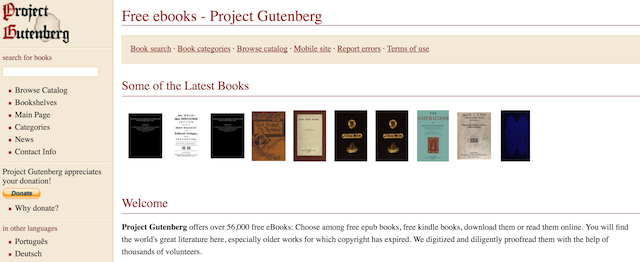
\includegraphics{images/gutenberg.png}
\caption{}
\end{figure}

    \begin{Verbatim}[commandchars=\\\{\}]
{\color{incolor}In [{\color{incolor}255}]:} \PY{n}{url} \PY{o}{=} \PY{l+s+s2}{\PYZdq{}}\PY{l+s+s2}{http://www.gutenberg.org/files/15784/15784\PYZhy{}0.txt}\PY{l+s+s2}{\PYZdq{}}
\end{Verbatim}


    \begin{Verbatim}[commandchars=\\\{\}]
{\color{incolor}In [{\color{incolor}256}]:} \PY{n}{response} \PY{o}{=} \PY{n}{requests}\PY{o}{.}\PY{n}{get}\PY{p}{(}\PY{n}{url}\PY{p}{)}
\end{Verbatim}


    \begin{Verbatim}[commandchars=\\\{\}]
{\color{incolor}In [{\color{incolor}257}]:} \PY{n+nb}{type}\PY{p}{(}\PY{n}{response}\PY{p}{)}
\end{Verbatim}


\begin{Verbatim}[commandchars=\\\{\}]
{\color{outcolor}Out[{\color{outcolor}257}]:} requests.models.Response
\end{Verbatim}
            
    \begin{Verbatim}[commandchars=\\\{\}]
{\color{incolor}In [{\color{incolor}258}]:} \PY{n}{soup\PYZus{}dos} \PY{o}{=} \PY{n}{BeautifulSoup}\PY{p}{(}\PY{n}{response}\PY{o}{.}\PY{n}{content}\PY{p}{,} \PY{l+s+s2}{\PYZdq{}}\PY{l+s+s2}{html.parser}\PY{l+s+s2}{\PYZdq{}}\PY{p}{)}
\end{Verbatim}


    \begin{Verbatim}[commandchars=\\\{\}]
{\color{incolor}In [{\color{incolor}259}]:} \PY{n+nb}{len}\PY{p}{(}\PY{n}{soup\PYZus{}dos}\PY{p}{)}
\end{Verbatim}


\begin{Verbatim}[commandchars=\\\{\}]
{\color{outcolor}Out[{\color{outcolor}259}]:} 1
\end{Verbatim}
            
    \begin{Verbatim}[commandchars=\\\{\}]
{\color{incolor}In [{\color{incolor}260}]:} \PY{n}{dos\PYZus{}text} \PY{o}{=} \PY{n}{soup\PYZus{}dos}\PY{o}{.}\PY{n}{get\PYZus{}text}\PY{p}{(}\PY{p}{)}
\end{Verbatim}


    \begin{Verbatim}[commandchars=\\\{\}]
{\color{incolor}In [{\color{incolor}261}]:} \PY{n+nb}{type}\PY{p}{(}\PY{n}{dos\PYZus{}text}\PY{p}{)}
\end{Verbatim}


\begin{Verbatim}[commandchars=\\\{\}]
{\color{outcolor}Out[{\color{outcolor}261}]:} str
\end{Verbatim}
            
    \begin{Verbatim}[commandchars=\\\{\}]
{\color{incolor}In [{\color{incolor}262}]:} \PY{n+nb}{len}\PY{p}{(}\PY{n}{dos\PYZus{}text}\PY{p}{)}
\end{Verbatim}


\begin{Verbatim}[commandchars=\\\{\}]
{\color{outcolor}Out[{\color{outcolor}262}]:} 550924
\end{Verbatim}
            
    \begin{Verbatim}[commandchars=\\\{\}]
{\color{incolor}In [{\color{incolor}266}]:} \PY{n}{dos\PYZus{}text}\PY{p}{[}\PY{p}{:}\PY{l+m+mi}{100}\PY{p}{]}
\end{Verbatim}


\begin{Verbatim}[commandchars=\\\{\}]
{\color{outcolor}Out[{\color{outcolor}266}]:} 'The Project Gutenberg EBook of The Chronology of Ancient Kingdoms Amended\textbackslash{}r\textbackslash{}nby Isaac Newton\textbackslash{}r\textbackslash{}n\textbackslash{}r\textbackslash{}nThis e'
\end{Verbatim}
            
    \subsubsection{Analyzing the Text with
NLTK}\label{analyzing-the-text-with-nltk}

The Natural Language Toolkit is a popular Python library for text
analysis. We will use it to split the text into individual
words(tokens), and create a plot of the frequency distribution of the
tokens.

    \begin{Verbatim}[commandchars=\\\{\}]
{\color{incolor}In [{\color{incolor}272}]:} \PY{k+kn}{from} \PY{n+nn}{nltk} \PY{k}{import} \PY{n}{word\PYZus{}tokenize}
          \PY{n}{tokens} \PY{o}{=} \PY{n}{word\PYZus{}tokenize}\PY{p}{(}\PY{n}{dos\PYZus{}text}\PY{p}{)}
\end{Verbatim}


    \begin{Verbatim}[commandchars=\\\{\}]
{\color{incolor}In [{\color{incolor}273}]:} \PY{n}{tokens}\PY{p}{[}\PY{p}{:}\PY{l+m+mi}{10}\PY{p}{]}
\end{Verbatim}


\begin{Verbatim}[commandchars=\\\{\}]
{\color{outcolor}Out[{\color{outcolor}273}]:} ['The',
           'Project',
           'Gutenberg',
           'EBook',
           'of',
           'The',
           'Chronology',
           'of',
           'Ancient',
           'Kingdoms']
\end{Verbatim}
            
    \begin{Verbatim}[commandchars=\\\{\}]
{\color{incolor}In [{\color{incolor}274}]:} \PY{n}{text} \PY{o}{=} \PY{n}{nltk}\PY{o}{.}\PY{n}{Text}\PY{p}{(}\PY{n}{tokens}\PY{p}{)}
\end{Verbatim}


    \begin{Verbatim}[commandchars=\\\{\}]
{\color{incolor}In [{\color{incolor}275}]:} \PY{n}{text}\PY{p}{[}\PY{p}{:}\PY{l+m+mi}{10}\PY{p}{]}
\end{Verbatim}


\begin{Verbatim}[commandchars=\\\{\}]
{\color{outcolor}Out[{\color{outcolor}275}]:} ['The',
           'Project',
           'Gutenberg',
           'EBook',
           'of',
           'The',
           'Chronology',
           'of',
           'Ancient',
           'Kingdoms']
\end{Verbatim}
            
    \begin{Verbatim}[commandchars=\\\{\}]
{\color{incolor}In [{\color{incolor}279}]:} \PY{n}{fdist} \PY{o}{=} \PY{n}{nltk}\PY{o}{.}\PY{n}{FreqDist}\PY{p}{(}\PY{n}{text}\PY{p}{)}
\end{Verbatim}


    \begin{Verbatim}[commandchars=\\\{\}]
{\color{incolor}In [{\color{incolor}287}]:} \PY{n+nb}{type}\PY{p}{(}\PY{n}{fdist}\PY{p}{)}
\end{Verbatim}


\begin{Verbatim}[commandchars=\\\{\}]
{\color{outcolor}Out[{\color{outcolor}287}]:} nltk.probability.FreqDist
\end{Verbatim}
            
    \begin{Verbatim}[commandchars=\\\{\}]
{\color{incolor}In [{\color{incolor} }]:} \PY{n}{lowered} \PY{o}{=} 
\end{Verbatim}


    \begin{Verbatim}[commandchars=\\\{\}]
{\color{incolor}In [{\color{incolor}281}]:} \PY{n}{fdist}\PY{o}{.}\PY{n}{most\PYZus{}common}\PY{p}{(}\PY{l+m+mi}{50}\PY{p}{)}
\end{Verbatim}


\begin{Verbatim}[commandchars=\\\{\}]
{\color{outcolor}Out[{\color{outcolor}281}]:} [(',', 8704),
           ('the', 7568),
           ('and', 5062),
           ('of', 5017),
           ('.', 3525),
           ('in', 1805),
           ('to', 1508),
           (';', 1200),
           (':', 1158),
           ('[', 1023),
           (']', 1023),
           ('that', 1004),
           ('by', 970),
           ('was', 941),
           ('a', 804),
           ('his', 703),
           ('with', 612),
           ('or', 588),
           ('years', 567),
           ('from', 531),
           ('for', 482),
           ('were', 455),
           ('their', 405),
           ('is', 394),
           ('he', 392),
           ('this', 389),
           ('year', 384),
           ('\_Egypt\_', 380),
           ('King', 378),
           ('which', 373),
           ('as', 373),
           ('at', 357),
           ('after', 348),
           ('they', 345),
           ('into', 342),
           ('it', 341),
           ('who', 322),
           ('l.', 313),
           ('son', 310),
           ('be', 303),
           ('Reign', 290),
           ('before', 284),
           ('Kings', 265),
           ('first', 261),
           ('about', 258),
           ('had', 250),
           ('not', 250),
           ('but', 242),
           ('The', 236),
           ('one', 235)]
\end{Verbatim}
            
    \begin{Verbatim}[commandchars=\\\{\}]
{\color{incolor}In [{\color{incolor}286}]:} \PY{n}{fdist}\PY{p}{[}\PY{l+s+s1}{\PYZsq{}}\PY{l+s+s1}{blood}\PY{l+s+s1}{\PYZsq{}}\PY{p}{]}
\end{Verbatim}


\begin{Verbatim}[commandchars=\\\{\}]
{\color{outcolor}Out[{\color{outcolor}286}]:} 5
\end{Verbatim}
            
    \begin{Verbatim}[commandchars=\\\{\}]
{\color{incolor}In [{\color{incolor}291}]:} \PY{n}{fdist} \PY{o}{=} \PY{n}{nltk}\PY{o}{.}\PY{n}{FreqDist}\PY{p}{(}\PY{n}{word}\PY{o}{.}\PY{n}{lower}\PY{p}{(}\PY{p}{)} \PY{k}{for} \PY{n}{word} \PY{o+ow}{in} \PY{n}{word\PYZus{}tokenize}\PY{p}{(}\PY{n}{dos\PYZus{}text}\PY{p}{)}\PY{p}{)}
\end{Verbatim}


    \begin{Verbatim}[commandchars=\\\{\}]
{\color{incolor}In [{\color{incolor}295}]:} \PY{n}{plt}\PY{o}{.}\PY{n}{figure}\PY{p}{(}\PY{p}{)}
          \PY{n}{fdist}\PY{o}{.}\PY{n}{plot}\PY{p}{(}\PY{l+m+mi}{30}\PY{p}{)}
\end{Verbatim}


    
    \begin{verbatim}
<IPython.core.display.Javascript object>
    \end{verbatim}

    
    
    \begin{verbatim}
<IPython.core.display.HTML object>
    \end{verbatim}

    
    \begin{Verbatim}[commandchars=\\\{\}]
{\color{incolor}In [{\color{incolor}297}]:} \PY{n}{plt}\PY{o}{.}\PY{n}{figure}\PY{p}{(}\PY{p}{)}
          \PY{n}{fdist}\PY{o}{.}\PY{n}{plot}\PY{p}{(}\PY{l+m+mi}{30}\PY{p}{,} \PY{n}{cumulative}\PY{o}{=}\PY{k+kc}{True}\PY{p}{)}
\end{Verbatim}


    
    \begin{verbatim}
<IPython.core.display.Javascript object>
    \end{verbatim}

    
    
    \begin{verbatim}
<IPython.core.display.HTML object>
    \end{verbatim}

    

    % Add a bibliography block to the postdoc
    
    
    
    \end{document}
